% 高一123_行知中学_10月月考.tex
%   —— 高一上数学“2026-2027 年行知中学高一上 10 月月考”（试卷版/答案版）
% 试卷版：xelatex 高一123_行知中学_10月月考.tex
% 答案版：xelatex "\def\isanswer{1}% 高一123_行知中学_10月月考.tex
%   —— 高一上数学“2026-2027 年行知中学高一上 10 月月考”（试卷版/答案版）
% 试卷版：xelatex 高一123_行知中学_10月月考.tex
% 答案版：xelatex "\def\isanswer{1}% 高一123_行知中学_10月月考.tex
%   —— 高一上数学“2026-2027 年行知中学高一上 10 月月考”（试卷版/答案版）
% 试卷版：xelatex 高一123_行知中学_10月月考.tex
% 答案版：xelatex "\def\isanswer{1}% 高一123_行知中学_10月月考.tex
%   —— 高一上数学“2026-2027 年行知中学高一上 10 月月考”（试卷版/答案版）
% 试卷版：xelatex 高一123_行知中学_10月月考.tex
% 答案版：xelatex "\def\isanswer{1}\input{高一123_行知中学_10月月考.tex}"
% 紧凑版：xelatex "\def\iscompact{1}\input{高一123_行知中学_10月月考.tex}"
%
% 原始材料：微信公众号“魔都数学加油站”文章，作者破晓，2026-11-09 17:52 发布；
% 连载“27学年高一123”，原文标题“27学年高一123——2026-2027年上海市行知中学高一上10月月考”；
% 原文链接：https://mp.weixin.qq.com/s/GV4SWBLUJrBhMQwo22FVzg。
% 正文为 14 张 PNG 页（第 7、9、11、13、14 页 2560×3620，其余 4762×6735），
% 题目下印有【答案】或【解析】，为讲评版。
% 题目、解析均据原图转录；卷面红色水印及公众号页脚未录入。
% 全卷 3 张插图：第 5 题的坐标示意图、第 17 题的文氏图（均属题干，三版都出）、
% 第 20 题 (2) 的 $t=\lvert x^2-1\rvert$ 图象（属解析，仅答案版出）；
% 都取原卷截图去水印、2× LANCZOS 放大，见 figures/gao123_q5.png、
% figures/gao123_q17.png、figures/gao123_q20.png。
%
% 卷首标题：原卷印作“2026-2027 年行知中学高一上 10 月月考”（公众号标题中的“上海市”
% 卷面标题行没有，本稿照卷面），年份区间按全稿惯例排 en dash；原卷未印副标题，本稿按题目内容
% 标为“集合与常用逻辑用语、不等式”（与 110／111／113／116／118／120 同）。
%
% 与原卷的排版差异：
%   ① 原文从第 3 题起，填空题编号为 3—12、选择题为 13—16、解答题为 17—21，本稿保留原题号；
%   ② 原卷每题下直接印【解析】／【答案】，本稿按全稿惯例置于答案版；第 3 题只印【答案】、
%      另提 \ans{}；选择题答案在解析末句“故选 …”，括号内留空；
%   ③ 原卷未印副标题，本稿按“知识模块”口径补出；
%   ④ 原卷填空横线按全稿惯例排为 \blankline[4.4em]；选择题括号排 \mbox{（\quad）}、
%      选项段前按惯例加 \keepwithprev；解答题不留作答区（原卷为讲评版，与 109—122 同）；
%   ⑤ 原卷数集排斜体 $R$／$Z$（第 9 题作粗体 $\mathbf{R}$），按全稿惯例改 \R／\Z；
%      绝对值按全稿惯例排 \lvert…\rvert，集合描述竖线排 \mid；单位 km、h 原卷排斜体，
%      本稿按正体照排；补集照原卷上划线排 \overline{B}、\overline{A}。
%
% 判别式与子集符号：第 16 题解析的 $\triangle=b^2-4c<0$、第 20 题 (1) ① 的 $\triangle<0$
%   均作等边、扁的 \triangle；第 20 题 ② 两处 cases 与 (3) 的 $\Delta\geqslant0$／$\Delta>0$
%   作等腰、高的 \Delta，逐处照录、不统一；第 15 题选项与第 17 题 (2) 的 $\subseteq$
%   印有下划线，照录 \subseteq。
%
% 原卷存疑照录：
%   第 4 题解析“若 $-\lvert a\rvert=0$，则 $a=0$，则 $A=\{0,-1,0\}$”以元素重复说明互异性；
%   第 5 题解析“当 $a^2+b^2=400^2+b^2<500^2$”等式左边 $a^2$ 与 $400^2$ 并用；
%   第 9 题解析“解得 $a>1$ 得 $a<\dfrac13$”（按平方不等式应为 $a>1$ 或 $a<\dfrac13$）；
%   第 12 题解析“所以 $-\dfrac1{2^a}\cdot\dfrac1{2^b}\geqslant-\dfrac14$”带负号起论；
%   第 17 题 (1) 解析把阴影部分（实为 $A\cap\overline B$）印作 $\overline{A\cap B}$；
%   第 18 题 (2) 解析作“$n<1$，所以 $n-1<0$”，与题设 $m<1$ 字母不一致；
%   第 20 题 (2) 的情形编号由 ①、② 直接跳到 ④（缺 ③）；
%   第 21 题 (2) 解析“$\lvert a_1-x_1\rvert+\cdots+\lvert a_i-x_i\rvert\leqslant n$”
%   末项下标作 $i$（按上下文应为 $n$）。以上均照录加注。
%
% 行数核对：逐题数 \step 条数，合计 176 条（Q3：0；Q4：6；Q5：5；Q6：5；Q7：4；
% Q8：6；Q9：5；Q10：5；Q11：10；Q12：6；Q13：9；Q14：1；Q15：5；Q16：21；
% Q17：8；Q18：14；Q19：10；Q20：26；Q21：30），与原卷印刷行逐题相等
% （cases 块作一个印刷行计）。第 3 题只印【答案】，提 \ans{}，不计入 \step 账。
%
\documentclass[a4paper,11pt]{article}
\usepackage{common}

\begin{document}

\examtitlest[3]{2026--2027 年行知中学高一上 10 月月考}{集合与常用逻辑用语、不等式}

\bigsec{一、填空题}

\begin{enumerate}
\setcounter{enumi}{2}

\item 写出命题“存在实数 $x$、$y$、$z$，使 $x<y$ 或 $y<z$.”的否定\blankline[4.4em].

\ifanswer
\ans{任意实数 $x$、$y$、$z$，使得 $x\geqslant y$ 且 $y\geqslant z$}
\fi

\item 若集合 $\{0,-1,2a\}=\{a-1,-\lvert a\rvert,a+1\}$，实数 $a$ 的值为\blankline[4.4em].

\ifanswer
\solbegin
\step{令 $A=\{0,-1,2a\}$,$B=\{a-1,-\lvert a\rvert,a+1\}$，}
\step{因为 $\{0,-1,2a\}=\{a-1,-\lvert a\rvert,a+1\}$，}
\step{若 $a-1=0$，则 $a=1$，则 $A=\{0,-1,2\}$,$B=\{0,-1,2\}$，满足要求；}
\step{若 $-\lvert a\rvert=0$，则 $a=0$，则 $A=\{0,-1,0\}$，不满足集合元素的互异性；}% 原卷以 $A=\{0,-1,0\}$ 说明互异性，照录
\step{若 $a+1=0$，则 $a=-1$，则 $A=\{0,-1,-2\}$,$B=\{0,-1,-2\}$，满足要求；}
\step{故实数 $a$ 的值为 $\pm1$.}
\solend
\fi

\needvspace{7cm}
\item 如图，据气象部门预报，在距离某码头南偏东 $45^\circ$ 方向 $400\sqrt2$ km 处的热带
风暴中心正在以 $20$km/h 的速度向正北方向移动，距风暴中心 $500$km 以内
的地区都将受到影响. 以上预报估计，该码头将受到热带风暴的影响时长大
约为\blankline[4.4em]$h$.

\begin{center}
% 图取原卷截图（第 1 页题干右侧）、去水印后 2× LANCZOS 放大，本稿移至题干之后
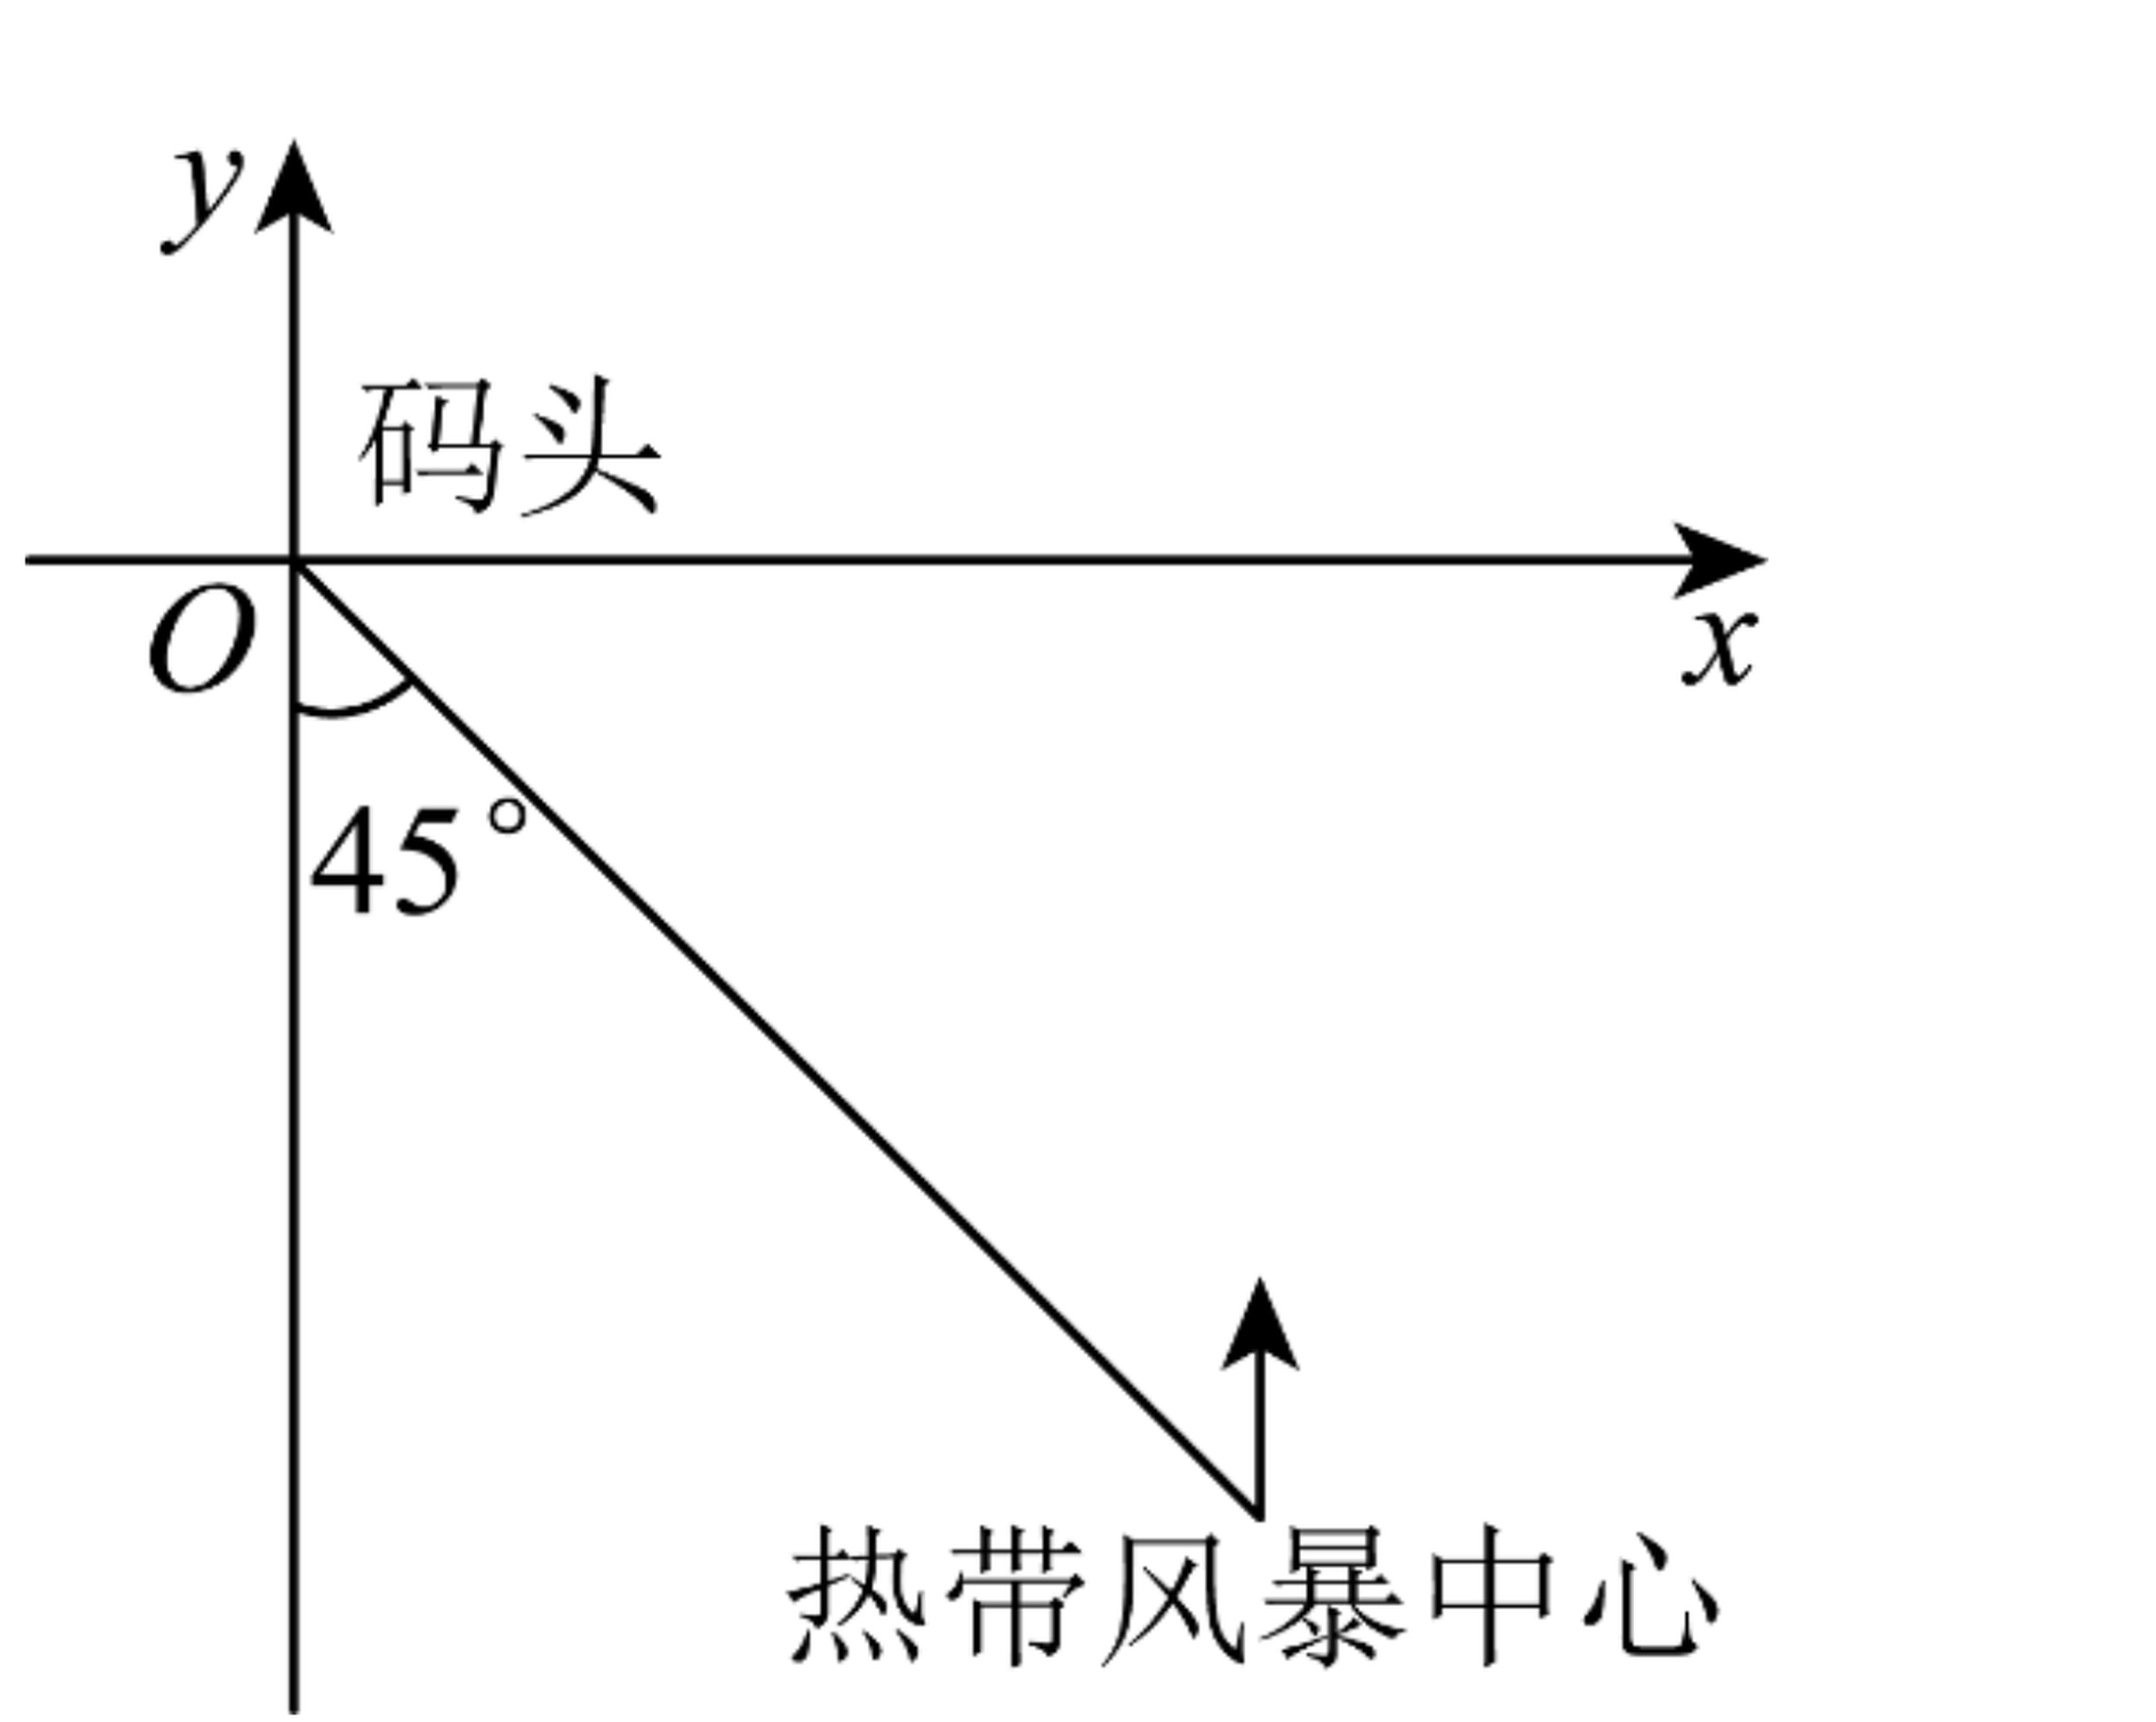
\includegraphics[width=0.36\textwidth]{figures/gao123_q5.png}
\end{center}

\ifanswer
\solbegin
\step{设风暴中心的坐标为 $(a,b)$，}
\step{由题意得 $a=400\sqrt2\times\cos45^\circ=400$，当 $a^2+b^2=400^2+b^2<500^2$，}% 原卷 $a^2$ 与 $400^2$ 并用，照录
\step{即 $-300<b<300$ 时，码头将受到风暴影响，}
\step{$\dfrac{300-(-300)}{20}=30h$，则码头受到风暴影响的时长为 30 小时，}
\step{所以由预报估计，该码头将受到热带风暴的影响时长大约为 30 小时.}
\solend
\fi

\item 已知 $a$、$b$、$c$ 为常数，若不等式 $\dfrac{ax-b}{x-c}\geqslant0$ 的解集为 $[-1,1)$，则不等式 $ax+b<0$ 的解集为\blankline[4.4em].

\ifanswer
\solbegin
\step{不等式 $\dfrac{ax-b}{x-c}\geqslant0$ 可化为 $(ax-b)(x-c)\geqslant0$ 且 $x-c\neq0$，}
\step{即 $a\left(x-\dfrac ba\right)(x-c)\geqslant0$ 且 $x\neq c$，}
\step{因为不等式 $\dfrac{ax-b}{x-c}\geqslant0$ 的解集为 $[-1,1)$，所以 $a<0$，且 $\dfrac ba=-1$,$c=1$，}
\step{即 $b=-a$，所以不等式 $ax+b<0$ 可化为 $ax-a<0$，又因为 $a<0$，所以 $x-1>0$，}
\step{解得 $x>1$，所以不等式 $ax+b<0$ 的解集为 $(1,+\infty)$.}
\solend
\fi

\item 已知实数 $a$、$b$ 满足 $ab=32$，且 $\log_2a=\log_b16$，则 $a+b$ 的值为\blankline[4.4em].

\ifanswer
\solbegin
\step{由 $\log_2a=\log_b16$，得 $\log_2a=\dfrac{\log_216}{\log_2b}$，则 $\log_2a\cdot\log_2b=4$，}
\step{由 $ab=32$，得 $\log_2a+\log_2b=\log_2ab=5$，}
\step{得 $\log_2a=1$,$\log_2b=4$ 或 $\log_2a=4$,$\log_2b=1$，}
\step{因此 $a=2$,$b=16$ 或 $a=16$,$b=2$，所以 $a+b=18$.}
\solend
\fi

\item 已知实数 $a$、$b$ 满足 $-3<a+2b<2$，$-1<2a-b<4$，则 $a+b$ 的取值范围为\blankline[4.4em].

\ifanswer
\solbegin
\step{设 $a+b=m(a+2b)+n(2a-b)=(m+2n)a+(2m-n)b$，}
\step{所以 $\begin{cases}m+2n=1\\2m-n=1\end{cases}$，解得 $n=\dfrac15$,$m=\dfrac35$，所以 $a+b=\dfrac35(a+2b)+\dfrac15(2a-b)$，}
\step{因为 $-3<(a+2b)<2$，$-1<2a-b<4$，}
\step{所以 $-\dfrac95<\dfrac35(a+2b)<\dfrac65$，$-\dfrac15<\dfrac15(2a-b)<\dfrac45$，}
\step{相加得 $-2<\dfrac35(a+2b)+\dfrac15(2a-b)<2$，即 $-2<a+b<2$，}
\step{故 $a+b$ 的取值范围为 $(-2,2)$.}
\solend
\fi

\item 存在 $x\in\R$ 使不等式 $\lvert2x-a\rvert<\lvert2a-1\rvert-2\lvert x\rvert$ 成立，则实数 $a$ 的取值范围是\blankline[4.4em].

\ifanswer
\solbegin
\step{存在 $x\in\R$，不等式 $\lvert2x-a\rvert<\lvert2a-1\rvert-2\lvert x\rvert$ 成立，}
\step{变形即 $\lvert2x-a\rvert+2\lvert x\rvert<\lvert2a-1\rvert$ 成立，}
\step{由于 $\lvert2x-a\rvert+\lvert2x\rvert\geqslant\lvert(2x-a)-2x\rvert=\lvert a\rvert$，当且仅当 $2x(2x-a)\leqslant0$ 时取等号，}
\step{因此有 $\lvert a\rvert<\lvert2a-1\rvert$，两边平方 $a^2<(2a-1)^2$，解得 $a>1$ 得 $a<\dfrac13$，}% 原卷“解得 a>1 得 a<1/3”，照录
\step{即实数 $a$ 的取值范围是 $\left(-\infty,\dfrac13\right)\cup(1,+\infty)$.}
\solend
\fi

\item 已知集合 $A=\{(x,y)\mid x^2+mx-y+2=0\}$，$B=\{(x,y)\mid x-y+1=0,0\leqslant x\leqslant3\}$，若集合 $A\cap B$ 的子集个数为 $2$，则实数 $m$ 的取值范围为\blankline[4.4em].

\ifanswer
\solbegin
\step{因为集合 $A\cap B$ 的子集个数为 $2$，所以 $A\cap B$ 的元素有一个，}
\step{即 $\begin{cases}x^2+mx-y+2=0\\x-y+1=0\end{cases}$ 在 $x\in[0,3]$ 上只有一个解，}
\step{即 $x^2+(m-1)x+1=0$ 在 $[0,3]$ 上只有一个解，}
\step{即 $1-m=x+\dfrac1x$ 在 $[0,3]$ 上只有一个解，}
\step{结合对勾函数的性质得 $1-m=2$ 或 $1-m>\dfrac{10}{3}$，解得 $m=-1$ 或 $m<-\dfrac73$.}
\solend
\fi

\item $[x]$ 表示不超过 $x$ 的最大整数，则集合 $A=\left\{y\,\middle\vert\,y=\left[\dfrac{x^2}{100}\right],x=1,2,3,\cdots,100\right\}$ 中的元素个数为\blankline[4.4em].

\ifanswer
\solbegin
\step{记 $a_k=\left[\dfrac{k^2}{100}\right](k=1,2,\cdots,100)$，$a_k$ 随 $k$ 增大而单调不减.}
\step{当 $k\geqslant50$ 时，$\dfrac{(k+1)^2}{100}-\dfrac{k^2}{100}=\dfrac{2k+1}{100}\geqslant\dfrac{101}{100}>1$，所以 $a_{k+1}\geqslant a_k+1$，}
\step{即 $a_{50}$、$a_{51}$、$\cdots$、$a_{100}$ 两两互异.}
\step{又 $a_{50}=\left[\dfrac{2500}{100}\right]=25$、$a_{100}=100$，这一段共 $100-50+1=51$ 个互异的值，}
\step{且都大于等于 $25$.}
\step{当 $k\leqslant49$ 时，$\dfrac{(k+1)^2}{100}-\dfrac{k^2}{100}=\dfrac{2k+1}{100}\leqslant\dfrac{99}{100}<1$，即 $a_k$ 每次至多增加 $1$；}
\step{又 $a_1=0$、$a_{49}=\left[\dfrac{2401}{100}\right]=24$，}
\step{故 $a_1$、$a_2$、$\cdots$、$a_{49}$ 依次取遍 $0$，$1$，$2$，$\cdots$，$24$，共 $25$ 个值.}
\step{两段取值范围互不重叠（前段不超过 $24$、后段不小于 $25$），}
\step{所以集合 $A$ 中共有 $25+51=76$ 个元素.}
\solend
\fi

\item 若实数 $a$、$b$、$c$ 满足 $\dfrac1{2^a}+\dfrac1{2^b}=1$，$\dfrac1{2^{a+b}}+\dfrac1{2^{b+c}}+\dfrac1{2^{a+c}}=1$，则 $c$ 的最大值是\blankline[4.4em].

\ifanswer
\solbegin
\step{因为 $\dfrac1{2^a}+\dfrac1{2^b}=1$，}
\step{由基本不等式得 $1=\dfrac1{2^a}+\dfrac1{2^b}\geqslant2\sqrt{\dfrac1{2^a}\cdot\dfrac1{2^b}}$（当且仅当 $a=b=1$ 时取等号），}
\step{所以 $\dfrac1{2^a}\cdot\dfrac1{2^b}\leqslant\dfrac14$，所以 $-\dfrac1{2^a}\cdot\dfrac1{2^b}\geqslant-\dfrac14$，}% 原卷带负号起论，照录
\step{因为 $\dfrac1{2^{a+b}}+\dfrac1{2^{b+c}}+\dfrac1{2^{a+c}}=1$，$\dfrac1{2^{b+c}}+\dfrac1{2^{a+c}}=\dfrac1{2^c}\left(\dfrac1{2^a}+\dfrac1{2^b}\right)=\dfrac1{2^c}$，}
\step{所以 $\dfrac1{2^c}=1-\dfrac1{2^{a+b}}\geqslant\dfrac34$，所以 $2^c\leqslant\dfrac43$，所以 $c\leqslant\log_2\dfrac43=2-\log_23$，}
\step{故 $c$ 的最大值是 $2-\log_23$.}
\solend
\fi

\end{enumerate}

\bigsec{二、选择题}

\begin{enumerate}
\setcounter{enumi}{12}

\item 下列运用等式或不等式的性质变形中，正确的是\mbox{（\quad）}

\keepwithprev
A. 如果 $a=b$，那么 $\dfrac ac=\dfrac bc$\qquad\qquad B. 如果 $\dfrac1a<\dfrac1b<0$，那么 $a-\dfrac1a>b-\dfrac1b$

C. 如果 $a>b$，那么 $\dfrac1a<\dfrac1b$\qquad\qquad D. 如果 $a>b>0$，$m\in\R$，那么 $\dfrac ba<\dfrac{b+m}{a+m}$

\ifanswer
\solbegin
\step{对于 $A$，若 $c=0$，$A$ 错误；}
\step{对于 $B$，若 $\dfrac1a<\dfrac1b<0$，则 $0>a>b$，$-\dfrac1a>-\dfrac1b>0$，}
\step{所以 $a-\dfrac1a>b-\dfrac1b$，$B$ 正确；}
\step{对于 $C$，$a>0$，$b<0$ 时，$C$ 错误；}
\step{对于 $D$，$\dfrac{b+m}{a+m}-\dfrac ba=\dfrac{ab+am}{a(a+m)}-\dfrac{ab+bm}{a(a+m)}=\dfrac{(a-b)m}{a(a+m)}$，}
\step{因为 $a>b>0$，所以 $a-b>0$，但 $m$、$a+m$ 的符号不确定，}
\step{当 $m=0$ 时，$\dfrac ba=\dfrac{b+m}{a+m}$，}
\step{当 $m(a+m)>0$ 时，$\dfrac ba<\dfrac{b+m}{a+m}$，当 $m(a+m)<0$ 时，$\dfrac ba>\dfrac{b+m}{a+m}$，$D$ 错误.}
\step{故选 $B$.}
\solend
\fi

\item “$a>b$”的一个必要非充分条件是\mbox{（\quad）}

\keepwithprev
A. $ac^2>bc^2$\qquad\quad B. $2^a>2^b$\qquad\quad C. $\left(\dfrac12\right)^{a-b}\leqslant1$\qquad\quad D. $a^3>b^3$

\ifanswer
\solbegin
\step{即“$a>b$”能推出选项，但选项不能推出“$a>b$”，故选 $C$.}
\solend
\fi

\item 若 $A=\left\{x\,\middle\vert\,x=\dfrac k6+1,k\in\Z\right\}$，$B=\left\{x\,\middle\vert\,x=\dfrac k3+\dfrac12,k\in\Z\right\}$，$C=\left\{x\,\middle\vert\,x=\dfrac{2k}{3}+\dfrac12,k\in\Z\right\}$，则这三个集合间的关系是\mbox{（\quad）}

\keepwithprev
A. $A\subseteq B\subseteq C$\qquad\quad B. $A\subseteq C\subseteq B$\qquad\quad C. $C\subseteq B\subseteq A$\qquad\quad D. $C\subseteq A\subseteq B$

\ifanswer
\solbegin
\step{若 $x\in C$，则存在 $k_0\in\Z$，使 $x=\dfrac{2k_0}{3}+\dfrac12$，}
\step{又 $2k_0\in\Z$，所以 $x\in B$，故 $C\subseteq B$，}
\step{若 $x\in B$，则存在 $k_1\in\Z$，使 $x=\dfrac{k_1}{3}+\dfrac12=\dfrac{2k_1-3}{6}+1$，}
\step{又 $2k_1-3\in\Z$，所以 $x\in A$，故 $B\subseteq A$，}
\step{又 $\dfrac43\in A$，$\dfrac43\notin B$，$\dfrac56\in B$，$\dfrac56\notin C$，所以 $C\subseteq B\subseteq A$，故选 $C$.}
\solend
\fi

\item 集合 $S=\{x\mid(x+a)(x^2+bx+c)=0\}$，$T=\{x\mid(ax+1)(cx^2+bx+1)=0\}$，其中 $a$、$b$、$c$ 为实数，若 $\lvert S\rvert$、$\lvert T\rvert$ 分别表示 $S$、$T$ 的元素个数，则下列结论中一定成立的是\mbox{（\quad）}

\keepwithprev
A. 若 $\lvert T\rvert=0$，则 $\lvert S\rvert=1$\qquad\qquad B. 若 $\lvert S\rvert=1$，则 $\lvert T\rvert=1$

C. 若 $\lvert S\rvert=2$，则 $\lvert T\rvert=2$\qquad\qquad D. 若 $\lvert T\rvert=3$，则 $\lvert S\rvert=2$

\ifanswer
\solbegin
\step{令 $f(x)=(x+a)(x^2+bx+c)$,$g(x)=(ax+1)(cx^2+bx+1)$，}
\step{对于选项 A，当 $\lvert T\rvert=0$ 时，方程 $g(x)=(ax+1)(cx^2+bx+1)=0$ 无实根，}
\step{当 $a=b=c=0$ 时，$f(x)=x^3$，由 $f(x)=0$ 得 $x=0$，此时 $\lvert S\rvert=1$；}
\step{当 $a=0$,$b^2-4c<0$ 时，$f(x)=x(x^2+bx+c)$，由 $f(x)=0$ 得 $x=0$，}
\step{此时 $\lvert S\rvert=1$，所以选项 A 正确；}
\step{对于选项 B，若 $\lvert S\rvert=1$，则 $f(x)=(x+a)(x^2+bx+c)=0$ 有且只有一根，}
\step{又 $x=-a$ 一定是 $f(x)=0$ 的根，所以 $\triangle=b^2-4c<0$，}
\step{又 $\triangle=b^2-4c<0$ 且 $a=0$ 时，$g(x)=(ax+1)(cx^2+bx+1)=0$ 无解，}
\step{此时 $\lvert T\rvert=0$，所以选项 B 错误，}
\step{对于选项 C，若 $\lvert S\rvert=2$ 时，则 $f(x)=(x+a)(x^2+bx+c)=0$ 有且只有 $2$ 根，}
\step{又 $x=-a$ 一定是 $f(x)=0$ 的根，}
\step{所以 $\triangle=b^2-4c=0$ 且 $a^2+ab+c\neq0$ 或 $\triangle=b^2-4c>0$ 且 $a^2+ab+c=0$，}
\step{当 $a=0$ 时，存在 $b$,$c$，使 $\triangle=b^2-4c=0$ 且 $a^2+ab+c\neq0$，}
\step{此时 $g(x)=(ax+1)(cx^2+bx+1)=0$ 只有一根，所以选项 C 错误，}
\step{对于选项 D，当 $\lvert T\rvert=3$ 时，方程 $g(x)=(ax+1)(cx^2+bx+1)=0$ 有三个根，}
\step{所以 $a\neq0$,$c\neq0$,$b^2-4c>0$，}
\step{设 $x_0$ 为 $g(x)=0$ 的一个根，即 $(ax_0+1)(cx_0^2+bx_0+1)=0$，}
\step{则 $x_0\neq0$，且 $f\left(\dfrac1{x_0}\right)=\left(\dfrac1{x_0}+a\right)\left(\dfrac1{x_0^2}+\dfrac1{x_0}b+c\right)=\dfrac1{x_0^3}g(x_0)=0$，}
\step{所以 $\dfrac1{x_0}$ 为方程 $f(x)=0$ 的根，故 $f(x)=0$ 有三个根，即 $\lvert T\rvert=3$ 时，}
\step{必有 $\lvert S\rvert=3$，所以选项 D 错误，}
\step{故选 $A$.}
\solend
\fi

\end{enumerate}

% 第 17 题是解答题第一题且带文氏图，守卫放在 \bigsec 之前，连节标题一起量页高
\needvspace{7cm}
\bigsec{三、解答题}

\begin{enumerate}
\setcounter{enumi}{16}

\item 设全集 $U=\R$，集合 $A=\{x\mid-2\leqslant x\leqslant4\}$，$B=\{x\mid x<-6$ 或 $x\geqslant2\}$.

（1）求图中阴影部分表示的集合；

（2）已知集合 $C=\{x\mid10-a<x<2a+1\}$，若 $\overline B\cap C=\varnothing$，求 $a$ 的取值范围.

\begin{center}
% 图取原卷截图（第 7 页题干右侧）、去水印后 2× LANCZOS 放大，本稿移至题干之后
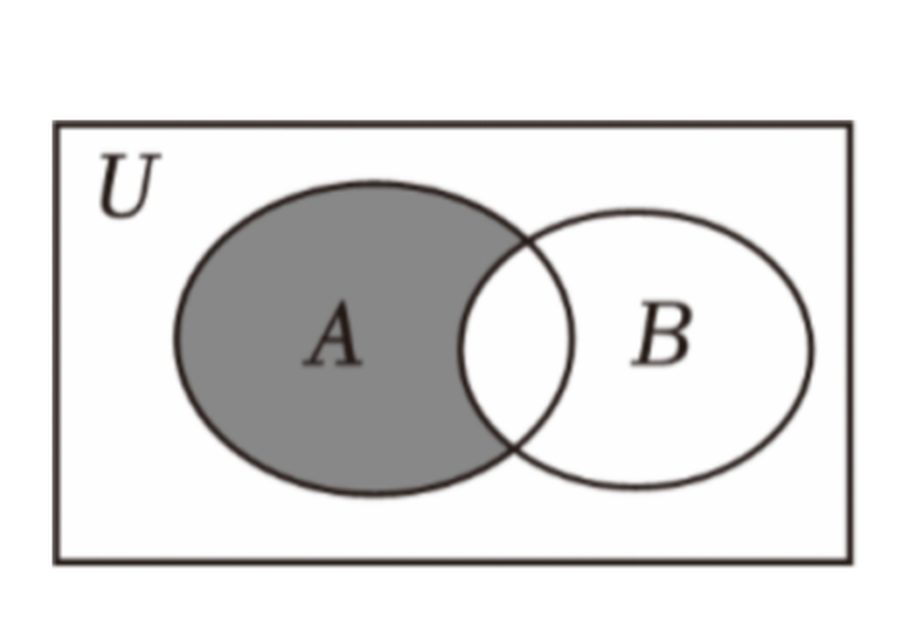
\includegraphics[width=0.34\textwidth]{figures/gao123_q17.png}
\end{center}

\ifanswer
\solbegin
\step{（1）$A\cap B=\{x\mid2\leqslant x\leqslant4\}$，}
\step{则图中阴影部分表示 $\overline{A\cap B}=\{x\mid-2\leqslant x<2\}$.}% 原卷把上划线盖在整个 $A\cap B$ 上，照录
\step{（2）由题意得 $\overline B=\{x\mid-6\leqslant x<2\}$，$C\subseteq B$，}
\step{所以当 $C=\varnothing$ 时，$10-a\geqslant2a+1$，解得 $a\leqslant3$，符合题意；}
\step{当 $C\neq\varnothing$ 时，$\begin{cases}10-a<2a+1\\2a+1\leqslant-6\end{cases}$ 或者 $\begin{cases}10-a<2a+1\\10-a\geqslant2\end{cases}$，}
\step{此时不等式组 $\begin{cases}10-a<2a+1\\2a+1\leqslant-6\end{cases}$ 无解，}
\step{不等式组 $\begin{cases}10-a<2a+1\\10-a\geqslant2\end{cases}$ 的解集为 $3<a\leqslant8$，}
\step{综上，$a$ 的取值范围为 $\{a\mid a\leqslant8\}$.}
\solend
\fi

\item (1) 求不等式：$\lvert x-1\rvert+\lvert x-2\rvert\leqslant5$ 的解集.

(2) 当 $m<1$ 时，解关于 $x$ 的不等式 $\dfrac{m(x-3)}{x+2}>1$.

\ifanswer
\solbegin
\step{(1) 当 $x<1$ 时，$\lvert x-1\rvert+\lvert x-2\rvert\leqslant5\Leftrightarrow-x+1+2-x\leqslant5$，}
\step{解得 $-1\leqslant x<1$；}
\step{当 $1\leqslant x\leqslant2$ 时，$\lvert x-1\rvert+\lvert x-2\rvert\leqslant5\Leftrightarrow x-1+2-x=1\leqslant5$ 恒成立，}
\step{所以 $1\leqslant x\leqslant2$；}
\step{当 $x>2$ 时，$\lvert x-1\rvert+\lvert x-2\rvert\leqslant5\Leftrightarrow x-1+x-2=2x-3\leqslant5$，}
\step{解得 $2<x\leqslant4$.}
\step{综上所述，不等式 $\lvert x-1\rvert+\lvert x-2\rvert\leqslant5$ 的解集为 $[-1,4]$.}
\step{(2) 原不等式变成 $\dfrac{(m-1)x-(3m+2)}{x+2}>0$，$n<1$，所以 $n-1<0$，}% 原卷作 $n<1$、$n-1<0$，与题设 $m<1$ 字母不一致，照录
\step{所以原不等式变成 $\dfrac{x-\dfrac{3m+2}{m-1}}{x+2}<0$，$\dfrac{3m+2}{m-1}-(-2)=\dfrac{5m}{m-1}$，}
\step{所以 $m<0$ 时，$\dfrac{5m}{m-1}>0$，$\dfrac{3m+2}{m-1}>-2$，}
\step{原不等式的解集为 $\left(-2,\dfrac{3m+2}{m-1}\right)$；}
\step{$m=0$ 时，原不等式变成 $1<0$，无解；}
\step{$0<m<1$ 时，$\dfrac{5m}{m-1}<0$，$\dfrac{3m+2}{m-1}<-2$，}
\step{原不等式的解集为 $\left(\dfrac{3m+2}{m-1},-2\right)$.}
\solend
\fi

\item 在园林博览会上，某公司带来了一种智能设备供采购商洽谈采购，并决定大量投放市场，已知该种设备年固定研发成本为 $50$ 万元，每生产一台需另投入 $100$ 元，设该公司一年内生产该设备 $x$ 万台且全部售完，每万台的销售收入 $G(x)$（万元）与年产量 $x$（万台）满足如下关系式：$G(x)=\begin{cases}180-x,0<x\leqslant20\\80+\dfrac{2000}{x}-\dfrac{8000}{x(x-1)},x>20\end{cases}$.

(1) 写出年利润 $W(x)$（万元）关于年产量 $x$（万台）的函数解析式；（利润 $=$ 销售收入 $-$ 成本）

(2) 当年产量为多少万台时，该公司获得的年利润最大，并求出最大利润.

\ifanswer
\solbegin
\step{(1) $W(x)=xG(x)-50-100x=\begin{cases}-50+80x-x^2,0<x\leqslant20\\-20x+1950-\dfrac{8000}{x-1},x>20\end{cases}$；}
\step{(2) 当 $0<x\leqslant20$ 时，$W(x)=-50+80x-x^2=-(x-40)^2+1550$，}
\step{由函数性质得当 $x\leqslant40$ 时严格增，所以当 $x=20$ 时，$W(x)_{max}=1150$，}
\step{当 $x>20$ 时，$W(x)=-20x+1950-\dfrac{8000}{x-1}=-20\left[(x-1)+\dfrac{400}{x-1}\right]+1930$，}
\step{$W(x)=-20\left[(x-1)+\dfrac{400}{x-1}\right]+1930\leqslant-20\times2\sqrt{(x-1)\cdot\dfrac{400}{x-1}}+1930$}
\step{$=1130$，当且仅当 $x-1=\dfrac{400}{x-1}$，即 $x=21$ 时取等号，}
\step{所以 $W(x)_{max}=1130$，}
\step{因为 $1150>1130$，所以当 $x=20$ 时，$W(x)_{max}=1150$，}
\step{即当年产量为 $20$ 万台时，该公司获得的年利润最大，}
\step{最大利润为 $1150$ 万元.}
\solend
\fi

\item 关于 $x$ 的方程 $(x^2-1)^2-2k\lvert x^2-1\rvert+k+1=0(k\in\R)$.

(1) 若方程无实根，求 $k$ 的取值范围；

(2) 若方程有 $4$ 个不等实根，求 $k$ 的取值范围；

(3) 若 $k=a+b$，且满足 $\dfrac1{a+2b}+\dfrac1{a+3}=\dfrac12$，$a>0$，$b>0$，试判断方程根的个数.

\ifanswer
\solbegin
\step{(1) 关于 $x$ 的方程 $(x^2-1)^2-2k\lvert x^2-1\rvert+k+1=0(k\in\R)$，}
\step{令 $t=\lvert x^2-1\rvert$，则 $t\geqslant0$，则原方程转化为 $t^2-2kt+k+1=0(*)$，}
\step{因为关于 $x$ 的方程 $(x^2-1)^2-2k\lvert x^2-1\rvert+k+1=0(k\in\R)$ 无实根，}
\step{所以 $(*)$ 式无实根或实根均小于零，令 $f(t)=t^2-2kt+k+1$，}
\step{①若 $(*)$ 式无实根，则 $\triangle<0$，解得 $\dfrac{1-\sqrt5}{2}<k<\dfrac{1+\sqrt5}{2}$，}
\step{②两根均为负，则 $\begin{cases}\Delta\geqslant0\\t_{\text{对}}=k<0\\f(0)>0\end{cases}$，解得 $-1<k\leqslant\dfrac{1-\sqrt5}{2}$，}
\step{综合①②，得 $k$ 的取值范围是 $\left(-1,\dfrac{1+\sqrt5}{2}\right)$；}
\step{(2) 作函数 $t=\lvert x^2-1\rvert$ 的图象，}
\begin{center}
% 图取原卷截图（第 11 页解析内）、去水印后 2× LANCZOS 放大，仅答案版出
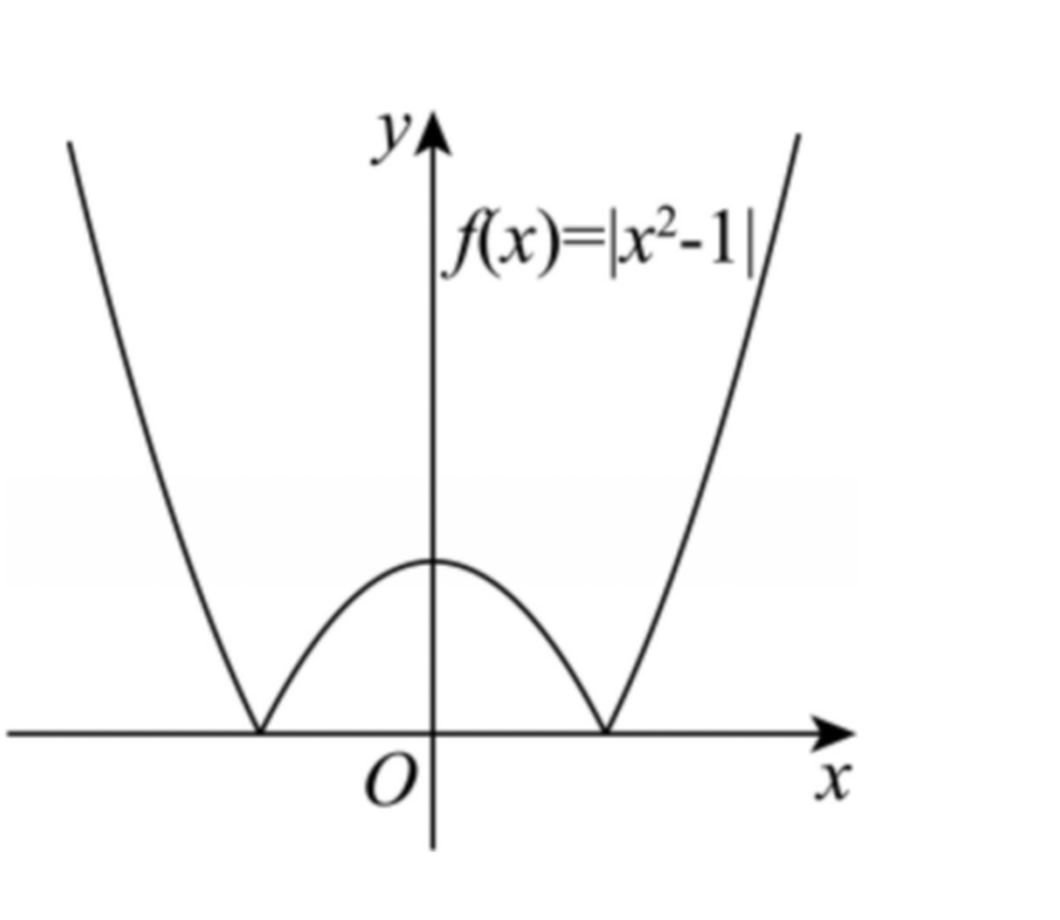
\includegraphics[width=0.40\textwidth]{figures/gao123_q20.png}
\end{center}
\step{$t=0$ 或 $t>1$ 时，每一个 $t$ 值对应 $2$ 个不同的 $x$ 值，}
\step{$t=1$ 时一个 $t$ 值对应 $3$ 个不同的 $x$ 值，}
\step{$0<t<1$ 时一个 $t$ 值对应 $4$ 个不同的 $x$ 值，}
\step{要使原方程有四个不等实根，}
\step{①$(*)$ 式一根为零，另一根大于 $1$，无解；}
\step{②$(*)$ 有两不等根且两根均大于 $1$，则 $\begin{cases}\Delta>0\\t_{\text{对}}=k>1\\f(1)>0\end{cases}$，解得 $\dfrac{1+\sqrt5}{2}<k<2$；}
\step{④$(*)$ 式有 $1$ 实根在 $(0,1)$ 之间，另一根小于零，}% 原卷由 ② 直接跳到 ④，缺 ③，照录
\step{则 $\begin{cases}f(0)<0\\f(1)>0\end{cases}$，所以 $\begin{cases}k+1<0\\2-k>0\end{cases}$，解得 $k<-1$，}
\step{综上所述，$k$ 取值范围为 $(-\infty,-1)\cup\left(\dfrac{1+\sqrt5}{2},2\right)$；}
\step{(3) 因为 $\dfrac1{a+2b}+\dfrac1{a+3}=\dfrac{a+2b+a+3}{(a+2b)(a+3)}=\dfrac{2(a+b)+3}{(a+2b)(a+3)}=\dfrac12$，}
\step{所以 $2(a+b)+3=\dfrac12(a+2b)(a+3)$，}
\step{因为 $a$、$b$ 为正实数，所以 $\dfrac12=\dfrac1{a+2b}+\dfrac1{a+3}\geqslant2\sqrt{\dfrac1{a+2b}\times\dfrac1{a+3}}$，}
\step{得 $\dfrac1{16}\geqslant\dfrac1{a+2b}\times\dfrac1{a+3}$，即 $(a+2b)(a+3)\geqslant16$，}
\step{所以 $2(a+b)+3\geqslant8$，即 $a+b\geqslant\dfrac52$，}
\step{当且仅当 $\dfrac1{a+2b}=\dfrac1{a+3}$ 即 $a=1$,$b=\dfrac32$ 时取等号，}
\step{故 $k\geqslant\dfrac52$，此时有 $\begin{cases}\Delta>0\\t_{\text{对}}=k>1\\f(0)>0,f(1)<0\end{cases}$，}
\step{故 $(*)$ 式有两不等实根且一根在 $(0,1)$ 之间，另一根大于 $1$，}
\step{故原方程有 $6$ 个实根.}
\solend
\fi

\item 设 $n$ 是不小于 $3$ 的正整数，集合 $S_n=\{(a_1,a_2,\cdots,a_n)\mid a_i\in\{0,1\},i=1,2,\cdots,n\}$，对于集合 $S_n$ 中任意两个元素 $A=(a_1,a_2,\cdots,a_n)$，$B=(b_1,b_2,\cdots,b_n)$.

定义 1：$A\cdot B=n-(\lvert a_1-b_1\rvert+\lvert a_2-b_2\rvert+\cdots+\lvert a_n-b_n\rvert)$，

定义 2：若 $A\cdot B=0$，则称互为相反元素，记作 $A=\overline B$ 或 $B=\overline A$.

(1) 若 $n=3$，$A=(0,1,0)$，$B=(1,1,0)$，试写出 $\overline A$、$\overline B$ 以及 $A\cdot B$ 的值；

(2) 若 $A$、$B\in S_n$，$A=(a_1,a_2,\cdots,a_n)$，$B=(b_1,b_2,\cdots,b_n)$，证明：$A\cdot B+\overline A\cdot B=n$；

(3) 设 $k$ 是小于 $n$ 的正奇数，至少含有两个元素的集合 $M\subseteq S_n$，且对于集合 $M$ 中任意两个不相同的元素 $A=(a_1,a_2,\cdots,a_n)$，$B=(b_1,b_2,\cdots,b_n)$，都有 $A\cdot B=n-k$，试求集合 $M$ 中元素个数的所有可能值.

\ifanswer
\solbegin
\step{(1) $\overline A=(1,0,1)$,$\overline B=(0,0,1)$,$\overline A\cdot\overline B=2$；}
\step{(2) 设 $A=(a_1,a_2,\cdots,a_n)$,$B=(b_1,b_2,\cdots,b_n)$,$\overline A=(x_1,x_2,\cdots,x_n)$，}
\step{由 $a_i$、$b_i$、$x_i\in\{0,1\}$，$i=1,2,\cdots,n$，得 $\lvert a_i-x_i\rvert\leqslant1$，$i=1,2,\cdots,n$，}
\step{所以 $\lvert a_1-x_1\rvert+\lvert a_2-x_2\rvert+\cdots+\lvert a_i-x_i\rvert\leqslant n$，}% 原卷末项下标作 $i$，照录
\step{当且仅当 $\lvert a_i-x_i\rvert=1$，$i=1,2,\cdots,n$，}
\step{即 $x_i=1-a_i$，$i=1,2,\cdots,n$ 时取等号.}
\step{由题意得 $A\cdot\overline A=n-(\lvert a_1-x_1\rvert+\lvert a_2-x_2\rvert+\cdots+\lvert a_n-x_n\rvert)=0$，}
\step{即 $\lvert a_1-x_1\rvert+\lvert a_2-x_2\rvert+\cdots+\lvert a_n-x_n\rvert=n$，}
\step{所以 $x_i=1-a_i$，$i=1,2,\cdots,n$，}
\step{$A\cdot B+\overline A\cdot B=2n-\sum\limits_{i=1}^n[\lvert a_i-b_i\rvert+(1-a_i)-b_i]$}
\step{$=2n-\sum\limits_{i=1}^n(\lvert1-b_i\rvert+\lvert0-b_i\rvert)=2n-\sum\limits_{i=1}^n(1-b_i+b_i)=2n-n=n$；}
\step{(3) 假设 $A=(a_1,a_2,\cdots,a_n)$，$B=(b_1,b_2,\cdots,b_n)$，$C=(c_1,c_2,\cdots,c_n)$}
\step{为集合 $M$ 中的三个不相同的元素，}
\step{则 $A\cdot B=n-(\lvert a_1-b_1\rvert+\lvert a_2-b_2\rvert+\cdots+\lvert a_n-b_n\rvert)=n-k$，}
\step{即 $\lvert a_1-b_1\rvert+\lvert a_2-b_2\rvert+\cdots+\lvert a_n-b_n\rvert=k$，}
\step{又由题意得 $\lvert a_i-b_i\rvert=0$ 或 $1$，$i=1,2,\cdots,n$，}
\step{$\lvert a_1-b_1\rvert$、$\lvert a_2-b_2\rvert$、$\cdots$、$\lvert a_n-b_n\rvert$ 恰有 $k$ 个 $1$，$n-k$ 个 $0$，}
\step{设其中 $k$ 个等于 $1$ 的项以此为 $a_{m_1}-b_{m_1}$,$a_{m_2}-b_{m_2}$,$\cdots$,$a_{m_k}-b_{m_k}$，}
\step{$n-k$ 个等于 $0$ 的项为 $a_{m_{k+1}}-b_{m_{k+1}}$,$a_{m_{k+2}}-b_{m_{k+2}}$,$\cdots$,$a_{m_n}-b_{m_n}$，}
\step{由题意得 $A\cdot C=n-(\lvert a_1-c_1\rvert+\lvert a_2-c_2\rvert+\cdots+\lvert a_n-c_n\rvert)=n-k$，}
\step{所以 $\sum\limits_{i=1}^k\lvert a_{m_i}-c_{m_i}\rvert+\sum\limits_{j=k+1}^n\lvert a_{m_j}-c_{m_j}\rvert=k$ ①，}
\step{同理 $\sum\limits_{i=1}^k\lvert b_{m_i}-c_{m_i}\rvert+\sum\limits_{j=k+1}^n\lvert b_{m_j}-c_{m_j}\rvert=k$ ②，}
\step{因为 $\lvert a_{m_{k+1}}-b_{m_{k+1}}\rvert=\lvert a_{m_{k+2}}-b_{m_{k+2}}\rvert=\cdots=\lvert a_{m_n}-b_{m_n}\rvert=0$，}
\step{所以 $\sum\limits_{j=k+1}^n\lvert a_{m_j}-c_{m_j}\rvert=\sum\limits_{j=k+1}^n\lvert b_{m_j}-c_{m_j}\rvert$，}
\step{由①$-$②得 $\sum\limits_{i=1}^k(\lvert a_{m_i}-c_{m_i}\rvert-\lvert b_{m_i}-c_{m_i}\rvert)=0$，}
\step{又 $\sum\limits_{i=1}^k(\lvert a_{m_i}-c_{m_i}\rvert-\lvert b_{m_i}-c_{m_i}\rvert)=\sum\limits_{i=1}^k(\lvert1-c_{m_i}\rvert-\lvert0-c_{m_i}\rvert)=k-2\sum\limits_{i=1}^k c_{m_i}$}
\step{为奇数，与 $\sum\limits_{i=1}^k(\lvert a_{m_i}-c_{m_i}\rvert-\lvert b_{m_i}-c_{m_i}\rvert)=0$ 矛盾，所以假设不成立，}
\step{即集合 $M$ 中至多有两个元素，}
\step{当 $M=\{(1,1,\cdots,1,0,0,\cdots,0),(0,0,\cdots,0)\}$ 时符合题意，}
\step{所以集合 $M$ 中元素的个数只可能是 $2$.}
\solend
\fi

\end{enumerate}

\end{document}
"
% 紧凑版：xelatex "\def\iscompact{1}% 高一123_行知中学_10月月考.tex
%   —— 高一上数学“2026-2027 年行知中学高一上 10 月月考”（试卷版/答案版）
% 试卷版：xelatex 高一123_行知中学_10月月考.tex
% 答案版：xelatex "\def\isanswer{1}\input{高一123_行知中学_10月月考.tex}"
% 紧凑版：xelatex "\def\iscompact{1}\input{高一123_行知中学_10月月考.tex}"
%
% 原始材料：微信公众号“魔都数学加油站”文章，作者破晓，2026-11-09 17:52 发布；
% 连载“27学年高一123”，原文标题“27学年高一123——2026-2027年上海市行知中学高一上10月月考”；
% 原文链接：https://mp.weixin.qq.com/s/GV4SWBLUJrBhMQwo22FVzg。
% 正文为 14 张 PNG 页（第 7、9、11、13、14 页 2560×3620，其余 4762×6735），
% 题目下印有【答案】或【解析】，为讲评版。
% 题目、解析均据原图转录；卷面红色水印及公众号页脚未录入。
% 全卷 3 张插图：第 5 题的坐标示意图、第 17 题的文氏图（均属题干，三版都出）、
% 第 20 题 (2) 的 $t=\lvert x^2-1\rvert$ 图象（属解析，仅答案版出）；
% 都取原卷截图去水印、2× LANCZOS 放大，见 figures/gao123_q5.png、
% figures/gao123_q17.png、figures/gao123_q20.png。
%
% 卷首标题：原卷印作“2026-2027 年行知中学高一上 10 月月考”（公众号标题中的“上海市”
% 卷面标题行没有，本稿照卷面），年份区间按全稿惯例排 en dash；原卷未印副标题，本稿按题目内容
% 标为“集合与常用逻辑用语、不等式”（与 110／111／113／116／118／120 同）。
%
% 与原卷的排版差异：
%   ① 原文从第 3 题起，填空题编号为 3—12、选择题为 13—16、解答题为 17—21，本稿保留原题号；
%   ② 原卷每题下直接印【解析】／【答案】，本稿按全稿惯例置于答案版；第 3 题只印【答案】、
%      另提 \ans{}；选择题答案在解析末句“故选 …”，括号内留空；
%   ③ 原卷未印副标题，本稿按“知识模块”口径补出；
%   ④ 原卷填空横线按全稿惯例排为 \blankline[4.4em]；选择题括号排 \mbox{（\quad）}、
%      选项段前按惯例加 \keepwithprev；解答题不留作答区（原卷为讲评版，与 109—122 同）；
%   ⑤ 原卷数集排斜体 $R$／$Z$（第 9 题作粗体 $\mathbf{R}$），按全稿惯例改 \R／\Z；
%      绝对值按全稿惯例排 \lvert…\rvert，集合描述竖线排 \mid；单位 km、h 原卷排斜体，
%      本稿按正体照排；补集照原卷上划线排 \overline{B}、\overline{A}。
%
% 判别式与子集符号：第 16 题解析的 $\triangle=b^2-4c<0$、第 20 题 (1) ① 的 $\triangle<0$
%   均作等边、扁的 \triangle；第 20 题 ② 两处 cases 与 (3) 的 $\Delta\geqslant0$／$\Delta>0$
%   作等腰、高的 \Delta，逐处照录、不统一；第 15 题选项与第 17 题 (2) 的 $\subseteq$
%   印有下划线，照录 \subseteq。
%
% 原卷存疑照录：
%   第 4 题解析“若 $-\lvert a\rvert=0$，则 $a=0$，则 $A=\{0,-1,0\}$”以元素重复说明互异性；
%   第 5 题解析“当 $a^2+b^2=400^2+b^2<500^2$”等式左边 $a^2$ 与 $400^2$ 并用；
%   第 9 题解析“解得 $a>1$ 得 $a<\dfrac13$”（按平方不等式应为 $a>1$ 或 $a<\dfrac13$）；
%   第 12 题解析“所以 $-\dfrac1{2^a}\cdot\dfrac1{2^b}\geqslant-\dfrac14$”带负号起论；
%   第 17 题 (1) 解析把阴影部分（实为 $A\cap\overline B$）印作 $\overline{A\cap B}$；
%   第 18 题 (2) 解析作“$n<1$，所以 $n-1<0$”，与题设 $m<1$ 字母不一致；
%   第 20 题 (2) 的情形编号由 ①、② 直接跳到 ④（缺 ③）；
%   第 21 题 (2) 解析“$\lvert a_1-x_1\rvert+\cdots+\lvert a_i-x_i\rvert\leqslant n$”
%   末项下标作 $i$（按上下文应为 $n$）。以上均照录加注。
%
% 行数核对：逐题数 \step 条数，合计 176 条（Q3：0；Q4：6；Q5：5；Q6：5；Q7：4；
% Q8：6；Q9：5；Q10：5；Q11：10；Q12：6；Q13：9；Q14：1；Q15：5；Q16：21；
% Q17：8；Q18：14；Q19：10；Q20：26；Q21：30），与原卷印刷行逐题相等
% （cases 块作一个印刷行计）。第 3 题只印【答案】，提 \ans{}，不计入 \step 账。
%
\documentclass[a4paper,11pt]{article}
\usepackage{common}

\begin{document}

\examtitlest[3]{2026--2027 年行知中学高一上 10 月月考}{集合与常用逻辑用语、不等式}

\bigsec{一、填空题}

\begin{enumerate}
\setcounter{enumi}{2}

\item 写出命题“存在实数 $x$、$y$、$z$，使 $x<y$ 或 $y<z$.”的否定\blankline[4.4em].

\ifanswer
\ans{任意实数 $x$、$y$、$z$，使得 $x\geqslant y$ 且 $y\geqslant z$}
\fi

\item 若集合 $\{0,-1,2a\}=\{a-1,-\lvert a\rvert,a+1\}$，实数 $a$ 的值为\blankline[4.4em].

\ifanswer
\solbegin
\step{令 $A=\{0,-1,2a\}$,$B=\{a-1,-\lvert a\rvert,a+1\}$，}
\step{因为 $\{0,-1,2a\}=\{a-1,-\lvert a\rvert,a+1\}$，}
\step{若 $a-1=0$，则 $a=1$，则 $A=\{0,-1,2\}$,$B=\{0,-1,2\}$，满足要求；}
\step{若 $-\lvert a\rvert=0$，则 $a=0$，则 $A=\{0,-1,0\}$，不满足集合元素的互异性；}% 原卷以 $A=\{0,-1,0\}$ 说明互异性，照录
\step{若 $a+1=0$，则 $a=-1$，则 $A=\{0,-1,-2\}$,$B=\{0,-1,-2\}$，满足要求；}
\step{故实数 $a$ 的值为 $\pm1$.}
\solend
\fi

\needvspace{7cm}
\item 如图，据气象部门预报，在距离某码头南偏东 $45^\circ$ 方向 $400\sqrt2$ km 处的热带
风暴中心正在以 $20$km/h 的速度向正北方向移动，距风暴中心 $500$km 以内
的地区都将受到影响. 以上预报估计，该码头将受到热带风暴的影响时长大
约为\blankline[4.4em]$h$.

\begin{center}
% 图取原卷截图（第 1 页题干右侧）、去水印后 2× LANCZOS 放大，本稿移至题干之后
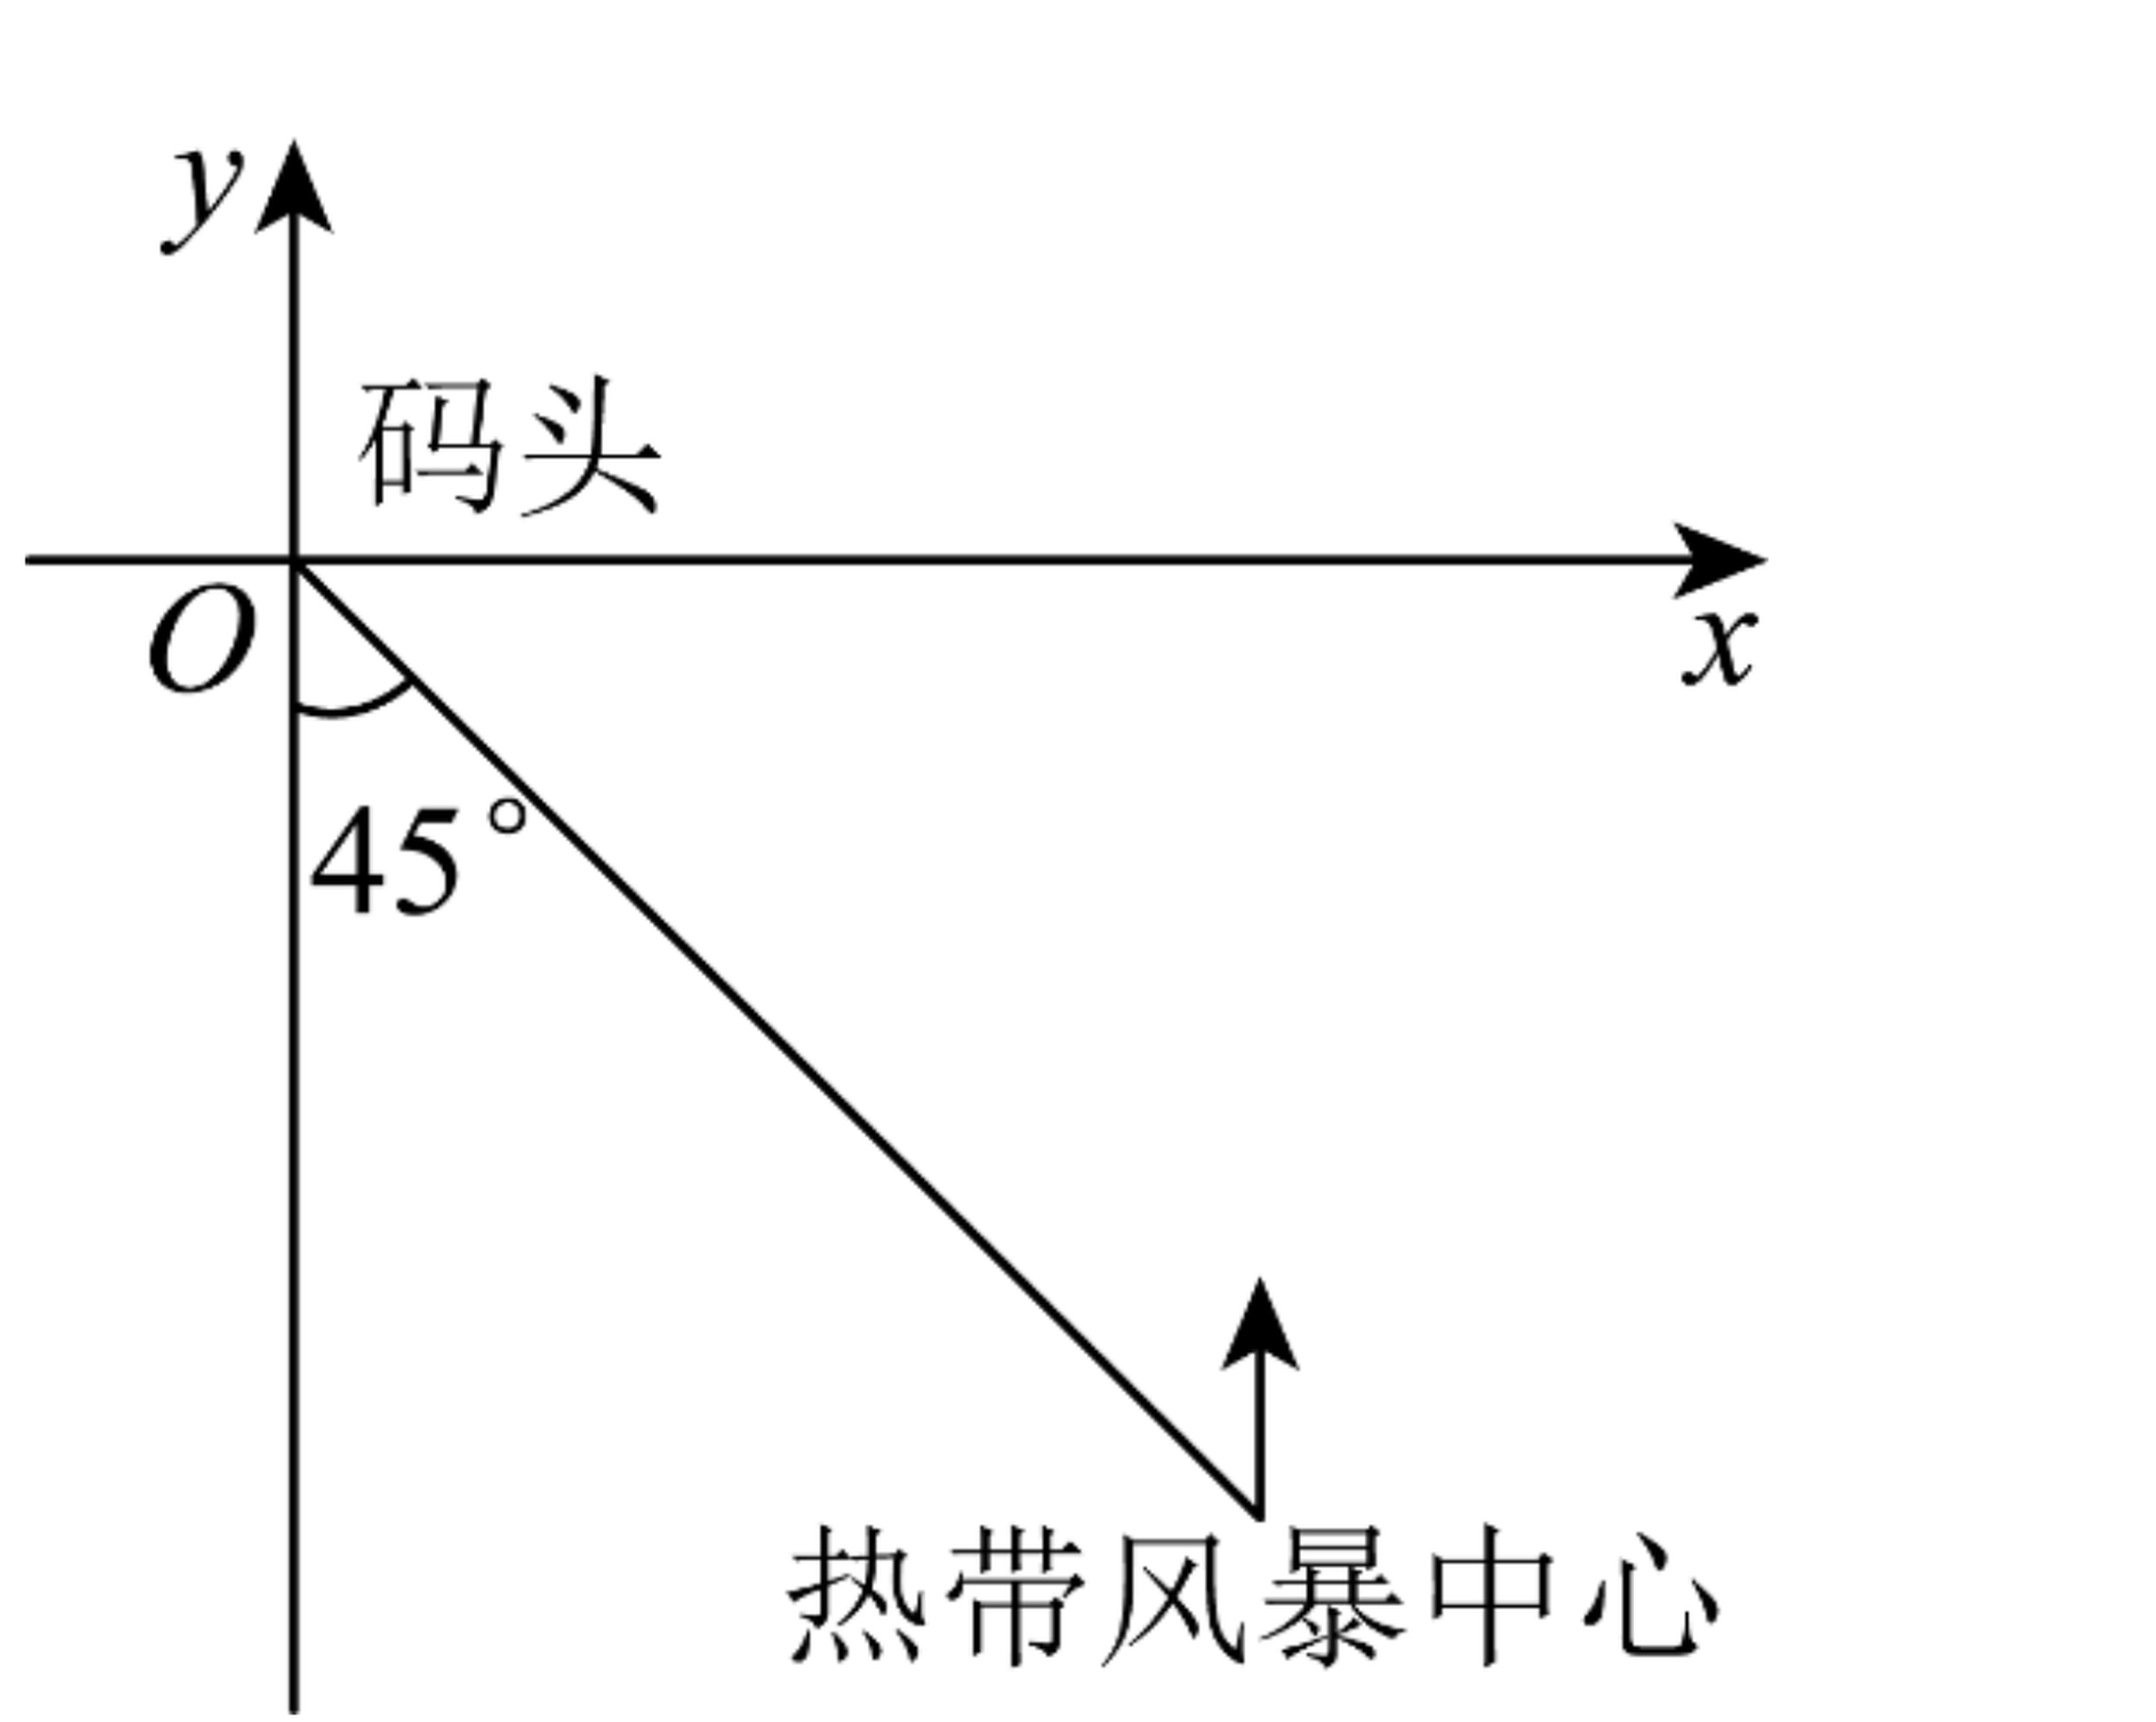
\includegraphics[width=0.36\textwidth]{figures/gao123_q5.png}
\end{center}

\ifanswer
\solbegin
\step{设风暴中心的坐标为 $(a,b)$，}
\step{由题意得 $a=400\sqrt2\times\cos45^\circ=400$，当 $a^2+b^2=400^2+b^2<500^2$，}% 原卷 $a^2$ 与 $400^2$ 并用，照录
\step{即 $-300<b<300$ 时，码头将受到风暴影响，}
\step{$\dfrac{300-(-300)}{20}=30h$，则码头受到风暴影响的时长为 30 小时，}
\step{所以由预报估计，该码头将受到热带风暴的影响时长大约为 30 小时.}
\solend
\fi

\item 已知 $a$、$b$、$c$ 为常数，若不等式 $\dfrac{ax-b}{x-c}\geqslant0$ 的解集为 $[-1,1)$，则不等式 $ax+b<0$ 的解集为\blankline[4.4em].

\ifanswer
\solbegin
\step{不等式 $\dfrac{ax-b}{x-c}\geqslant0$ 可化为 $(ax-b)(x-c)\geqslant0$ 且 $x-c\neq0$，}
\step{即 $a\left(x-\dfrac ba\right)(x-c)\geqslant0$ 且 $x\neq c$，}
\step{因为不等式 $\dfrac{ax-b}{x-c}\geqslant0$ 的解集为 $[-1,1)$，所以 $a<0$，且 $\dfrac ba=-1$,$c=1$，}
\step{即 $b=-a$，所以不等式 $ax+b<0$ 可化为 $ax-a<0$，又因为 $a<0$，所以 $x-1>0$，}
\step{解得 $x>1$，所以不等式 $ax+b<0$ 的解集为 $(1,+\infty)$.}
\solend
\fi

\item 已知实数 $a$、$b$ 满足 $ab=32$，且 $\log_2a=\log_b16$，则 $a+b$ 的值为\blankline[4.4em].

\ifanswer
\solbegin
\step{由 $\log_2a=\log_b16$，得 $\log_2a=\dfrac{\log_216}{\log_2b}$，则 $\log_2a\cdot\log_2b=4$，}
\step{由 $ab=32$，得 $\log_2a+\log_2b=\log_2ab=5$，}
\step{得 $\log_2a=1$,$\log_2b=4$ 或 $\log_2a=4$,$\log_2b=1$，}
\step{因此 $a=2$,$b=16$ 或 $a=16$,$b=2$，所以 $a+b=18$.}
\solend
\fi

\item 已知实数 $a$、$b$ 满足 $-3<a+2b<2$，$-1<2a-b<4$，则 $a+b$ 的取值范围为\blankline[4.4em].

\ifanswer
\solbegin
\step{设 $a+b=m(a+2b)+n(2a-b)=(m+2n)a+(2m-n)b$，}
\step{所以 $\begin{cases}m+2n=1\\2m-n=1\end{cases}$，解得 $n=\dfrac15$,$m=\dfrac35$，所以 $a+b=\dfrac35(a+2b)+\dfrac15(2a-b)$，}
\step{因为 $-3<(a+2b)<2$，$-1<2a-b<4$，}
\step{所以 $-\dfrac95<\dfrac35(a+2b)<\dfrac65$，$-\dfrac15<\dfrac15(2a-b)<\dfrac45$，}
\step{相加得 $-2<\dfrac35(a+2b)+\dfrac15(2a-b)<2$，即 $-2<a+b<2$，}
\step{故 $a+b$ 的取值范围为 $(-2,2)$.}
\solend
\fi

\item 存在 $x\in\R$ 使不等式 $\lvert2x-a\rvert<\lvert2a-1\rvert-2\lvert x\rvert$ 成立，则实数 $a$ 的取值范围是\blankline[4.4em].

\ifanswer
\solbegin
\step{存在 $x\in\R$，不等式 $\lvert2x-a\rvert<\lvert2a-1\rvert-2\lvert x\rvert$ 成立，}
\step{变形即 $\lvert2x-a\rvert+2\lvert x\rvert<\lvert2a-1\rvert$ 成立，}
\step{由于 $\lvert2x-a\rvert+\lvert2x\rvert\geqslant\lvert(2x-a)-2x\rvert=\lvert a\rvert$，当且仅当 $2x(2x-a)\leqslant0$ 时取等号，}
\step{因此有 $\lvert a\rvert<\lvert2a-1\rvert$，两边平方 $a^2<(2a-1)^2$，解得 $a>1$ 得 $a<\dfrac13$，}% 原卷“解得 a>1 得 a<1/3”，照录
\step{即实数 $a$ 的取值范围是 $\left(-\infty,\dfrac13\right)\cup(1,+\infty)$.}
\solend
\fi

\item 已知集合 $A=\{(x,y)\mid x^2+mx-y+2=0\}$，$B=\{(x,y)\mid x-y+1=0,0\leqslant x\leqslant3\}$，若集合 $A\cap B$ 的子集个数为 $2$，则实数 $m$ 的取值范围为\blankline[4.4em].

\ifanswer
\solbegin
\step{因为集合 $A\cap B$ 的子集个数为 $2$，所以 $A\cap B$ 的元素有一个，}
\step{即 $\begin{cases}x^2+mx-y+2=0\\x-y+1=0\end{cases}$ 在 $x\in[0,3]$ 上只有一个解，}
\step{即 $x^2+(m-1)x+1=0$ 在 $[0,3]$ 上只有一个解，}
\step{即 $1-m=x+\dfrac1x$ 在 $[0,3]$ 上只有一个解，}
\step{结合对勾函数的性质得 $1-m=2$ 或 $1-m>\dfrac{10}{3}$，解得 $m=-1$ 或 $m<-\dfrac73$.}
\solend
\fi

\item $[x]$ 表示不超过 $x$ 的最大整数，则集合 $A=\left\{y\,\middle\vert\,y=\left[\dfrac{x^2}{100}\right],x=1,2,3,\cdots,100\right\}$ 中的元素个数为\blankline[4.4em].

\ifanswer
\solbegin
\step{记 $a_k=\left[\dfrac{k^2}{100}\right](k=1,2,\cdots,100)$，$a_k$ 随 $k$ 增大而单调不减.}
\step{当 $k\geqslant50$ 时，$\dfrac{(k+1)^2}{100}-\dfrac{k^2}{100}=\dfrac{2k+1}{100}\geqslant\dfrac{101}{100}>1$，所以 $a_{k+1}\geqslant a_k+1$，}
\step{即 $a_{50}$、$a_{51}$、$\cdots$、$a_{100}$ 两两互异.}
\step{又 $a_{50}=\left[\dfrac{2500}{100}\right]=25$、$a_{100}=100$，这一段共 $100-50+1=51$ 个互异的值，}
\step{且都大于等于 $25$.}
\step{当 $k\leqslant49$ 时，$\dfrac{(k+1)^2}{100}-\dfrac{k^2}{100}=\dfrac{2k+1}{100}\leqslant\dfrac{99}{100}<1$，即 $a_k$ 每次至多增加 $1$；}
\step{又 $a_1=0$、$a_{49}=\left[\dfrac{2401}{100}\right]=24$，}
\step{故 $a_1$、$a_2$、$\cdots$、$a_{49}$ 依次取遍 $0$，$1$，$2$，$\cdots$，$24$，共 $25$ 个值.}
\step{两段取值范围互不重叠（前段不超过 $24$、后段不小于 $25$），}
\step{所以集合 $A$ 中共有 $25+51=76$ 个元素.}
\solend
\fi

\item 若实数 $a$、$b$、$c$ 满足 $\dfrac1{2^a}+\dfrac1{2^b}=1$，$\dfrac1{2^{a+b}}+\dfrac1{2^{b+c}}+\dfrac1{2^{a+c}}=1$，则 $c$ 的最大值是\blankline[4.4em].

\ifanswer
\solbegin
\step{因为 $\dfrac1{2^a}+\dfrac1{2^b}=1$，}
\step{由基本不等式得 $1=\dfrac1{2^a}+\dfrac1{2^b}\geqslant2\sqrt{\dfrac1{2^a}\cdot\dfrac1{2^b}}$（当且仅当 $a=b=1$ 时取等号），}
\step{所以 $\dfrac1{2^a}\cdot\dfrac1{2^b}\leqslant\dfrac14$，所以 $-\dfrac1{2^a}\cdot\dfrac1{2^b}\geqslant-\dfrac14$，}% 原卷带负号起论，照录
\step{因为 $\dfrac1{2^{a+b}}+\dfrac1{2^{b+c}}+\dfrac1{2^{a+c}}=1$，$\dfrac1{2^{b+c}}+\dfrac1{2^{a+c}}=\dfrac1{2^c}\left(\dfrac1{2^a}+\dfrac1{2^b}\right)=\dfrac1{2^c}$，}
\step{所以 $\dfrac1{2^c}=1-\dfrac1{2^{a+b}}\geqslant\dfrac34$，所以 $2^c\leqslant\dfrac43$，所以 $c\leqslant\log_2\dfrac43=2-\log_23$，}
\step{故 $c$ 的最大值是 $2-\log_23$.}
\solend
\fi

\end{enumerate}

\bigsec{二、选择题}

\begin{enumerate}
\setcounter{enumi}{12}

\item 下列运用等式或不等式的性质变形中，正确的是\mbox{（\quad）}

\keepwithprev
A. 如果 $a=b$，那么 $\dfrac ac=\dfrac bc$\qquad\qquad B. 如果 $\dfrac1a<\dfrac1b<0$，那么 $a-\dfrac1a>b-\dfrac1b$

C. 如果 $a>b$，那么 $\dfrac1a<\dfrac1b$\qquad\qquad D. 如果 $a>b>0$，$m\in\R$，那么 $\dfrac ba<\dfrac{b+m}{a+m}$

\ifanswer
\solbegin
\step{对于 $A$，若 $c=0$，$A$ 错误；}
\step{对于 $B$，若 $\dfrac1a<\dfrac1b<0$，则 $0>a>b$，$-\dfrac1a>-\dfrac1b>0$，}
\step{所以 $a-\dfrac1a>b-\dfrac1b$，$B$ 正确；}
\step{对于 $C$，$a>0$，$b<0$ 时，$C$ 错误；}
\step{对于 $D$，$\dfrac{b+m}{a+m}-\dfrac ba=\dfrac{ab+am}{a(a+m)}-\dfrac{ab+bm}{a(a+m)}=\dfrac{(a-b)m}{a(a+m)}$，}
\step{因为 $a>b>0$，所以 $a-b>0$，但 $m$、$a+m$ 的符号不确定，}
\step{当 $m=0$ 时，$\dfrac ba=\dfrac{b+m}{a+m}$，}
\step{当 $m(a+m)>0$ 时，$\dfrac ba<\dfrac{b+m}{a+m}$，当 $m(a+m)<0$ 时，$\dfrac ba>\dfrac{b+m}{a+m}$，$D$ 错误.}
\step{故选 $B$.}
\solend
\fi

\item “$a>b$”的一个必要非充分条件是\mbox{（\quad）}

\keepwithprev
A. $ac^2>bc^2$\qquad\quad B. $2^a>2^b$\qquad\quad C. $\left(\dfrac12\right)^{a-b}\leqslant1$\qquad\quad D. $a^3>b^3$

\ifanswer
\solbegin
\step{即“$a>b$”能推出选项，但选项不能推出“$a>b$”，故选 $C$.}
\solend
\fi

\item 若 $A=\left\{x\,\middle\vert\,x=\dfrac k6+1,k\in\Z\right\}$，$B=\left\{x\,\middle\vert\,x=\dfrac k3+\dfrac12,k\in\Z\right\}$，$C=\left\{x\,\middle\vert\,x=\dfrac{2k}{3}+\dfrac12,k\in\Z\right\}$，则这三个集合间的关系是\mbox{（\quad）}

\keepwithprev
A. $A\subseteq B\subseteq C$\qquad\quad B. $A\subseteq C\subseteq B$\qquad\quad C. $C\subseteq B\subseteq A$\qquad\quad D. $C\subseteq A\subseteq B$

\ifanswer
\solbegin
\step{若 $x\in C$，则存在 $k_0\in\Z$，使 $x=\dfrac{2k_0}{3}+\dfrac12$，}
\step{又 $2k_0\in\Z$，所以 $x\in B$，故 $C\subseteq B$，}
\step{若 $x\in B$，则存在 $k_1\in\Z$，使 $x=\dfrac{k_1}{3}+\dfrac12=\dfrac{2k_1-3}{6}+1$，}
\step{又 $2k_1-3\in\Z$，所以 $x\in A$，故 $B\subseteq A$，}
\step{又 $\dfrac43\in A$，$\dfrac43\notin B$，$\dfrac56\in B$，$\dfrac56\notin C$，所以 $C\subseteq B\subseteq A$，故选 $C$.}
\solend
\fi

\item 集合 $S=\{x\mid(x+a)(x^2+bx+c)=0\}$，$T=\{x\mid(ax+1)(cx^2+bx+1)=0\}$，其中 $a$、$b$、$c$ 为实数，若 $\lvert S\rvert$、$\lvert T\rvert$ 分别表示 $S$、$T$ 的元素个数，则下列结论中一定成立的是\mbox{（\quad）}

\keepwithprev
A. 若 $\lvert T\rvert=0$，则 $\lvert S\rvert=1$\qquad\qquad B. 若 $\lvert S\rvert=1$，则 $\lvert T\rvert=1$

C. 若 $\lvert S\rvert=2$，则 $\lvert T\rvert=2$\qquad\qquad D. 若 $\lvert T\rvert=3$，则 $\lvert S\rvert=2$

\ifanswer
\solbegin
\step{令 $f(x)=(x+a)(x^2+bx+c)$,$g(x)=(ax+1)(cx^2+bx+1)$，}
\step{对于选项 A，当 $\lvert T\rvert=0$ 时，方程 $g(x)=(ax+1)(cx^2+bx+1)=0$ 无实根，}
\step{当 $a=b=c=0$ 时，$f(x)=x^3$，由 $f(x)=0$ 得 $x=0$，此时 $\lvert S\rvert=1$；}
\step{当 $a=0$,$b^2-4c<0$ 时，$f(x)=x(x^2+bx+c)$，由 $f(x)=0$ 得 $x=0$，}
\step{此时 $\lvert S\rvert=1$，所以选项 A 正确；}
\step{对于选项 B，若 $\lvert S\rvert=1$，则 $f(x)=(x+a)(x^2+bx+c)=0$ 有且只有一根，}
\step{又 $x=-a$ 一定是 $f(x)=0$ 的根，所以 $\triangle=b^2-4c<0$，}
\step{又 $\triangle=b^2-4c<0$ 且 $a=0$ 时，$g(x)=(ax+1)(cx^2+bx+1)=0$ 无解，}
\step{此时 $\lvert T\rvert=0$，所以选项 B 错误，}
\step{对于选项 C，若 $\lvert S\rvert=2$ 时，则 $f(x)=(x+a)(x^2+bx+c)=0$ 有且只有 $2$ 根，}
\step{又 $x=-a$ 一定是 $f(x)=0$ 的根，}
\step{所以 $\triangle=b^2-4c=0$ 且 $a^2+ab+c\neq0$ 或 $\triangle=b^2-4c>0$ 且 $a^2+ab+c=0$，}
\step{当 $a=0$ 时，存在 $b$,$c$，使 $\triangle=b^2-4c=0$ 且 $a^2+ab+c\neq0$，}
\step{此时 $g(x)=(ax+1)(cx^2+bx+1)=0$ 只有一根，所以选项 C 错误，}
\step{对于选项 D，当 $\lvert T\rvert=3$ 时，方程 $g(x)=(ax+1)(cx^2+bx+1)=0$ 有三个根，}
\step{所以 $a\neq0$,$c\neq0$,$b^2-4c>0$，}
\step{设 $x_0$ 为 $g(x)=0$ 的一个根，即 $(ax_0+1)(cx_0^2+bx_0+1)=0$，}
\step{则 $x_0\neq0$，且 $f\left(\dfrac1{x_0}\right)=\left(\dfrac1{x_0}+a\right)\left(\dfrac1{x_0^2}+\dfrac1{x_0}b+c\right)=\dfrac1{x_0^3}g(x_0)=0$，}
\step{所以 $\dfrac1{x_0}$ 为方程 $f(x)=0$ 的根，故 $f(x)=0$ 有三个根，即 $\lvert T\rvert=3$ 时，}
\step{必有 $\lvert S\rvert=3$，所以选项 D 错误，}
\step{故选 $A$.}
\solend
\fi

\end{enumerate}

% 第 17 题是解答题第一题且带文氏图，守卫放在 \bigsec 之前，连节标题一起量页高
\needvspace{7cm}
\bigsec{三、解答题}

\begin{enumerate}
\setcounter{enumi}{16}

\item 设全集 $U=\R$，集合 $A=\{x\mid-2\leqslant x\leqslant4\}$，$B=\{x\mid x<-6$ 或 $x\geqslant2\}$.

（1）求图中阴影部分表示的集合；

（2）已知集合 $C=\{x\mid10-a<x<2a+1\}$，若 $\overline B\cap C=\varnothing$，求 $a$ 的取值范围.

\begin{center}
% 图取原卷截图（第 7 页题干右侧）、去水印后 2× LANCZOS 放大，本稿移至题干之后
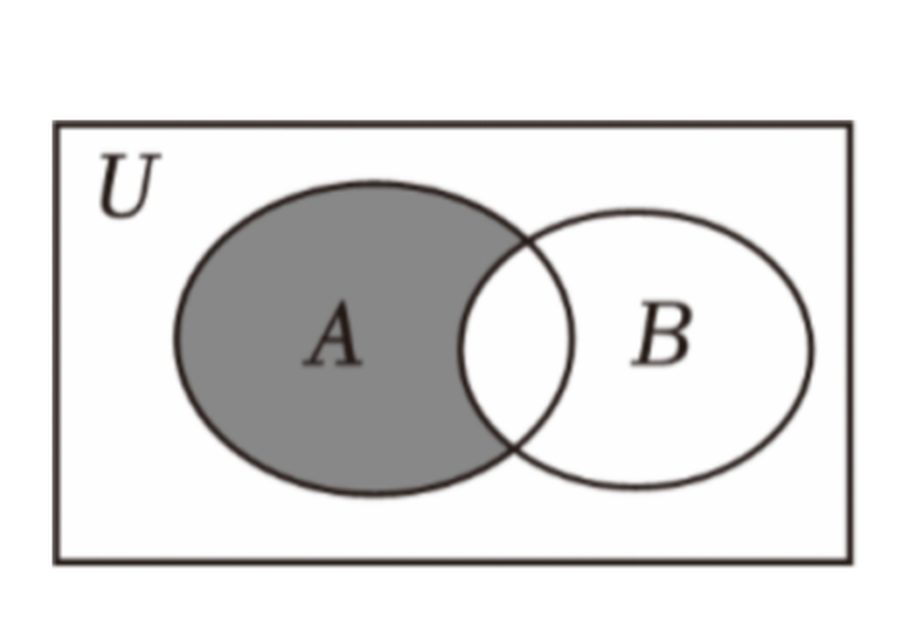
\includegraphics[width=0.34\textwidth]{figures/gao123_q17.png}
\end{center}

\ifanswer
\solbegin
\step{（1）$A\cap B=\{x\mid2\leqslant x\leqslant4\}$，}
\step{则图中阴影部分表示 $\overline{A\cap B}=\{x\mid-2\leqslant x<2\}$.}% 原卷把上划线盖在整个 $A\cap B$ 上，照录
\step{（2）由题意得 $\overline B=\{x\mid-6\leqslant x<2\}$，$C\subseteq B$，}
\step{所以当 $C=\varnothing$ 时，$10-a\geqslant2a+1$，解得 $a\leqslant3$，符合题意；}
\step{当 $C\neq\varnothing$ 时，$\begin{cases}10-a<2a+1\\2a+1\leqslant-6\end{cases}$ 或者 $\begin{cases}10-a<2a+1\\10-a\geqslant2\end{cases}$，}
\step{此时不等式组 $\begin{cases}10-a<2a+1\\2a+1\leqslant-6\end{cases}$ 无解，}
\step{不等式组 $\begin{cases}10-a<2a+1\\10-a\geqslant2\end{cases}$ 的解集为 $3<a\leqslant8$，}
\step{综上，$a$ 的取值范围为 $\{a\mid a\leqslant8\}$.}
\solend
\fi

\item (1) 求不等式：$\lvert x-1\rvert+\lvert x-2\rvert\leqslant5$ 的解集.

(2) 当 $m<1$ 时，解关于 $x$ 的不等式 $\dfrac{m(x-3)}{x+2}>1$.

\ifanswer
\solbegin
\step{(1) 当 $x<1$ 时，$\lvert x-1\rvert+\lvert x-2\rvert\leqslant5\Leftrightarrow-x+1+2-x\leqslant5$，}
\step{解得 $-1\leqslant x<1$；}
\step{当 $1\leqslant x\leqslant2$ 时，$\lvert x-1\rvert+\lvert x-2\rvert\leqslant5\Leftrightarrow x-1+2-x=1\leqslant5$ 恒成立，}
\step{所以 $1\leqslant x\leqslant2$；}
\step{当 $x>2$ 时，$\lvert x-1\rvert+\lvert x-2\rvert\leqslant5\Leftrightarrow x-1+x-2=2x-3\leqslant5$，}
\step{解得 $2<x\leqslant4$.}
\step{综上所述，不等式 $\lvert x-1\rvert+\lvert x-2\rvert\leqslant5$ 的解集为 $[-1,4]$.}
\step{(2) 原不等式变成 $\dfrac{(m-1)x-(3m+2)}{x+2}>0$，$n<1$，所以 $n-1<0$，}% 原卷作 $n<1$、$n-1<0$，与题设 $m<1$ 字母不一致，照录
\step{所以原不等式变成 $\dfrac{x-\dfrac{3m+2}{m-1}}{x+2}<0$，$\dfrac{3m+2}{m-1}-(-2)=\dfrac{5m}{m-1}$，}
\step{所以 $m<0$ 时，$\dfrac{5m}{m-1}>0$，$\dfrac{3m+2}{m-1}>-2$，}
\step{原不等式的解集为 $\left(-2,\dfrac{3m+2}{m-1}\right)$；}
\step{$m=0$ 时，原不等式变成 $1<0$，无解；}
\step{$0<m<1$ 时，$\dfrac{5m}{m-1}<0$，$\dfrac{3m+2}{m-1}<-2$，}
\step{原不等式的解集为 $\left(\dfrac{3m+2}{m-1},-2\right)$.}
\solend
\fi

\item 在园林博览会上，某公司带来了一种智能设备供采购商洽谈采购，并决定大量投放市场，已知该种设备年固定研发成本为 $50$ 万元，每生产一台需另投入 $100$ 元，设该公司一年内生产该设备 $x$ 万台且全部售完，每万台的销售收入 $G(x)$（万元）与年产量 $x$（万台）满足如下关系式：$G(x)=\begin{cases}180-x,0<x\leqslant20\\80+\dfrac{2000}{x}-\dfrac{8000}{x(x-1)},x>20\end{cases}$.

(1) 写出年利润 $W(x)$（万元）关于年产量 $x$（万台）的函数解析式；（利润 $=$ 销售收入 $-$ 成本）

(2) 当年产量为多少万台时，该公司获得的年利润最大，并求出最大利润.

\ifanswer
\solbegin
\step{(1) $W(x)=xG(x)-50-100x=\begin{cases}-50+80x-x^2,0<x\leqslant20\\-20x+1950-\dfrac{8000}{x-1},x>20\end{cases}$；}
\step{(2) 当 $0<x\leqslant20$ 时，$W(x)=-50+80x-x^2=-(x-40)^2+1550$，}
\step{由函数性质得当 $x\leqslant40$ 时严格增，所以当 $x=20$ 时，$W(x)_{max}=1150$，}
\step{当 $x>20$ 时，$W(x)=-20x+1950-\dfrac{8000}{x-1}=-20\left[(x-1)+\dfrac{400}{x-1}\right]+1930$，}
\step{$W(x)=-20\left[(x-1)+\dfrac{400}{x-1}\right]+1930\leqslant-20\times2\sqrt{(x-1)\cdot\dfrac{400}{x-1}}+1930$}
\step{$=1130$，当且仅当 $x-1=\dfrac{400}{x-1}$，即 $x=21$ 时取等号，}
\step{所以 $W(x)_{max}=1130$，}
\step{因为 $1150>1130$，所以当 $x=20$ 时，$W(x)_{max}=1150$，}
\step{即当年产量为 $20$ 万台时，该公司获得的年利润最大，}
\step{最大利润为 $1150$ 万元.}
\solend
\fi

\item 关于 $x$ 的方程 $(x^2-1)^2-2k\lvert x^2-1\rvert+k+1=0(k\in\R)$.

(1) 若方程无实根，求 $k$ 的取值范围；

(2) 若方程有 $4$ 个不等实根，求 $k$ 的取值范围；

(3) 若 $k=a+b$，且满足 $\dfrac1{a+2b}+\dfrac1{a+3}=\dfrac12$，$a>0$，$b>0$，试判断方程根的个数.

\ifanswer
\solbegin
\step{(1) 关于 $x$ 的方程 $(x^2-1)^2-2k\lvert x^2-1\rvert+k+1=0(k\in\R)$，}
\step{令 $t=\lvert x^2-1\rvert$，则 $t\geqslant0$，则原方程转化为 $t^2-2kt+k+1=0(*)$，}
\step{因为关于 $x$ 的方程 $(x^2-1)^2-2k\lvert x^2-1\rvert+k+1=0(k\in\R)$ 无实根，}
\step{所以 $(*)$ 式无实根或实根均小于零，令 $f(t)=t^2-2kt+k+1$，}
\step{①若 $(*)$ 式无实根，则 $\triangle<0$，解得 $\dfrac{1-\sqrt5}{2}<k<\dfrac{1+\sqrt5}{2}$，}
\step{②两根均为负，则 $\begin{cases}\Delta\geqslant0\\t_{\text{对}}=k<0\\f(0)>0\end{cases}$，解得 $-1<k\leqslant\dfrac{1-\sqrt5}{2}$，}
\step{综合①②，得 $k$ 的取值范围是 $\left(-1,\dfrac{1+\sqrt5}{2}\right)$；}
\step{(2) 作函数 $t=\lvert x^2-1\rvert$ 的图象，}
\begin{center}
% 图取原卷截图（第 11 页解析内）、去水印后 2× LANCZOS 放大，仅答案版出
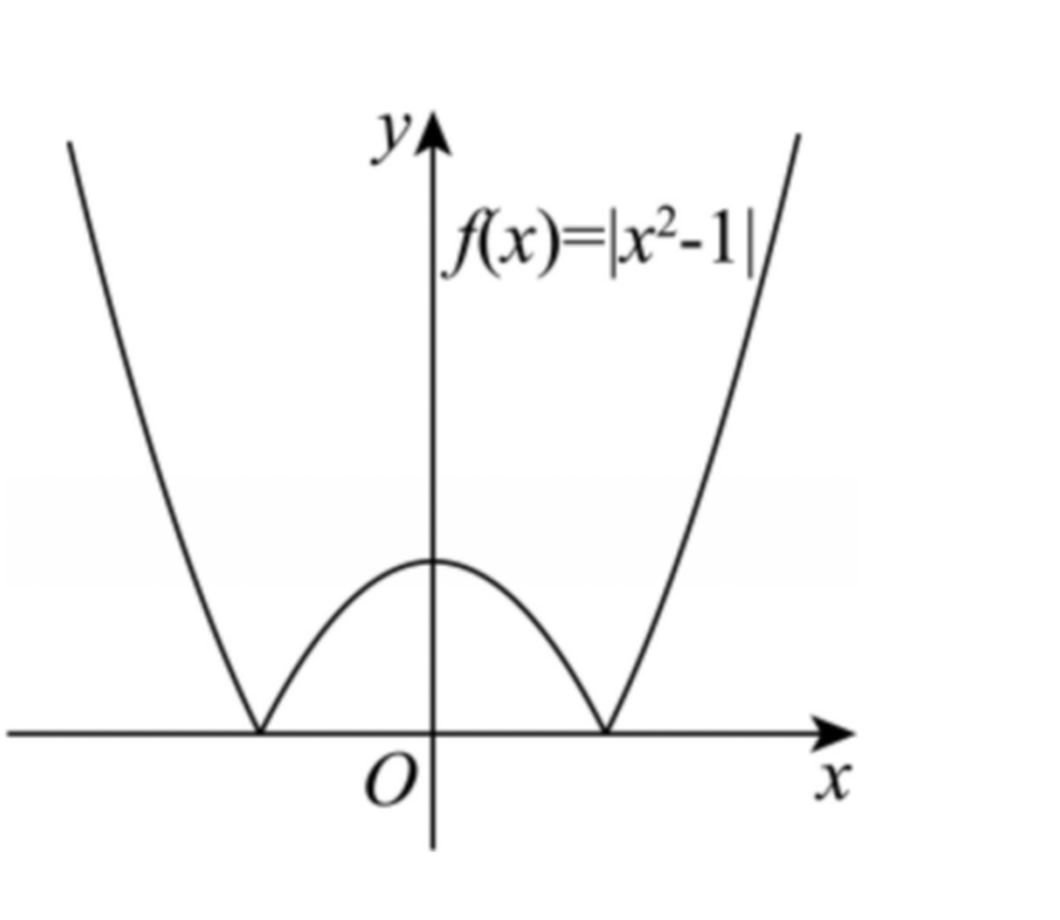
\includegraphics[width=0.40\textwidth]{figures/gao123_q20.png}
\end{center}
\step{$t=0$ 或 $t>1$ 时，每一个 $t$ 值对应 $2$ 个不同的 $x$ 值，}
\step{$t=1$ 时一个 $t$ 值对应 $3$ 个不同的 $x$ 值，}
\step{$0<t<1$ 时一个 $t$ 值对应 $4$ 个不同的 $x$ 值，}
\step{要使原方程有四个不等实根，}
\step{①$(*)$ 式一根为零，另一根大于 $1$，无解；}
\step{②$(*)$ 有两不等根且两根均大于 $1$，则 $\begin{cases}\Delta>0\\t_{\text{对}}=k>1\\f(1)>0\end{cases}$，解得 $\dfrac{1+\sqrt5}{2}<k<2$；}
\step{④$(*)$ 式有 $1$ 实根在 $(0,1)$ 之间，另一根小于零，}% 原卷由 ② 直接跳到 ④，缺 ③，照录
\step{则 $\begin{cases}f(0)<0\\f(1)>0\end{cases}$，所以 $\begin{cases}k+1<0\\2-k>0\end{cases}$，解得 $k<-1$，}
\step{综上所述，$k$ 取值范围为 $(-\infty,-1)\cup\left(\dfrac{1+\sqrt5}{2},2\right)$；}
\step{(3) 因为 $\dfrac1{a+2b}+\dfrac1{a+3}=\dfrac{a+2b+a+3}{(a+2b)(a+3)}=\dfrac{2(a+b)+3}{(a+2b)(a+3)}=\dfrac12$，}
\step{所以 $2(a+b)+3=\dfrac12(a+2b)(a+3)$，}
\step{因为 $a$、$b$ 为正实数，所以 $\dfrac12=\dfrac1{a+2b}+\dfrac1{a+3}\geqslant2\sqrt{\dfrac1{a+2b}\times\dfrac1{a+3}}$，}
\step{得 $\dfrac1{16}\geqslant\dfrac1{a+2b}\times\dfrac1{a+3}$，即 $(a+2b)(a+3)\geqslant16$，}
\step{所以 $2(a+b)+3\geqslant8$，即 $a+b\geqslant\dfrac52$，}
\step{当且仅当 $\dfrac1{a+2b}=\dfrac1{a+3}$ 即 $a=1$,$b=\dfrac32$ 时取等号，}
\step{故 $k\geqslant\dfrac52$，此时有 $\begin{cases}\Delta>0\\t_{\text{对}}=k>1\\f(0)>0,f(1)<0\end{cases}$，}
\step{故 $(*)$ 式有两不等实根且一根在 $(0,1)$ 之间，另一根大于 $1$，}
\step{故原方程有 $6$ 个实根.}
\solend
\fi

\item 设 $n$ 是不小于 $3$ 的正整数，集合 $S_n=\{(a_1,a_2,\cdots,a_n)\mid a_i\in\{0,1\},i=1,2,\cdots,n\}$，对于集合 $S_n$ 中任意两个元素 $A=(a_1,a_2,\cdots,a_n)$，$B=(b_1,b_2,\cdots,b_n)$.

定义 1：$A\cdot B=n-(\lvert a_1-b_1\rvert+\lvert a_2-b_2\rvert+\cdots+\lvert a_n-b_n\rvert)$，

定义 2：若 $A\cdot B=0$，则称互为相反元素，记作 $A=\overline B$ 或 $B=\overline A$.

(1) 若 $n=3$，$A=(0,1,0)$，$B=(1,1,0)$，试写出 $\overline A$、$\overline B$ 以及 $A\cdot B$ 的值；

(2) 若 $A$、$B\in S_n$，$A=(a_1,a_2,\cdots,a_n)$，$B=(b_1,b_2,\cdots,b_n)$，证明：$A\cdot B+\overline A\cdot B=n$；

(3) 设 $k$ 是小于 $n$ 的正奇数，至少含有两个元素的集合 $M\subseteq S_n$，且对于集合 $M$ 中任意两个不相同的元素 $A=(a_1,a_2,\cdots,a_n)$，$B=(b_1,b_2,\cdots,b_n)$，都有 $A\cdot B=n-k$，试求集合 $M$ 中元素个数的所有可能值.

\ifanswer
\solbegin
\step{(1) $\overline A=(1,0,1)$,$\overline B=(0,0,1)$,$\overline A\cdot\overline B=2$；}
\step{(2) 设 $A=(a_1,a_2,\cdots,a_n)$,$B=(b_1,b_2,\cdots,b_n)$,$\overline A=(x_1,x_2,\cdots,x_n)$，}
\step{由 $a_i$、$b_i$、$x_i\in\{0,1\}$，$i=1,2,\cdots,n$，得 $\lvert a_i-x_i\rvert\leqslant1$，$i=1,2,\cdots,n$，}
\step{所以 $\lvert a_1-x_1\rvert+\lvert a_2-x_2\rvert+\cdots+\lvert a_i-x_i\rvert\leqslant n$，}% 原卷末项下标作 $i$，照录
\step{当且仅当 $\lvert a_i-x_i\rvert=1$，$i=1,2,\cdots,n$，}
\step{即 $x_i=1-a_i$，$i=1,2,\cdots,n$ 时取等号.}
\step{由题意得 $A\cdot\overline A=n-(\lvert a_1-x_1\rvert+\lvert a_2-x_2\rvert+\cdots+\lvert a_n-x_n\rvert)=0$，}
\step{即 $\lvert a_1-x_1\rvert+\lvert a_2-x_2\rvert+\cdots+\lvert a_n-x_n\rvert=n$，}
\step{所以 $x_i=1-a_i$，$i=1,2,\cdots,n$，}
\step{$A\cdot B+\overline A\cdot B=2n-\sum\limits_{i=1}^n[\lvert a_i-b_i\rvert+(1-a_i)-b_i]$}
\step{$=2n-\sum\limits_{i=1}^n(\lvert1-b_i\rvert+\lvert0-b_i\rvert)=2n-\sum\limits_{i=1}^n(1-b_i+b_i)=2n-n=n$；}
\step{(3) 假设 $A=(a_1,a_2,\cdots,a_n)$，$B=(b_1,b_2,\cdots,b_n)$，$C=(c_1,c_2,\cdots,c_n)$}
\step{为集合 $M$ 中的三个不相同的元素，}
\step{则 $A\cdot B=n-(\lvert a_1-b_1\rvert+\lvert a_2-b_2\rvert+\cdots+\lvert a_n-b_n\rvert)=n-k$，}
\step{即 $\lvert a_1-b_1\rvert+\lvert a_2-b_2\rvert+\cdots+\lvert a_n-b_n\rvert=k$，}
\step{又由题意得 $\lvert a_i-b_i\rvert=0$ 或 $1$，$i=1,2,\cdots,n$，}
\step{$\lvert a_1-b_1\rvert$、$\lvert a_2-b_2\rvert$、$\cdots$、$\lvert a_n-b_n\rvert$ 恰有 $k$ 个 $1$，$n-k$ 个 $0$，}
\step{设其中 $k$ 个等于 $1$ 的项以此为 $a_{m_1}-b_{m_1}$,$a_{m_2}-b_{m_2}$,$\cdots$,$a_{m_k}-b_{m_k}$，}
\step{$n-k$ 个等于 $0$ 的项为 $a_{m_{k+1}}-b_{m_{k+1}}$,$a_{m_{k+2}}-b_{m_{k+2}}$,$\cdots$,$a_{m_n}-b_{m_n}$，}
\step{由题意得 $A\cdot C=n-(\lvert a_1-c_1\rvert+\lvert a_2-c_2\rvert+\cdots+\lvert a_n-c_n\rvert)=n-k$，}
\step{所以 $\sum\limits_{i=1}^k\lvert a_{m_i}-c_{m_i}\rvert+\sum\limits_{j=k+1}^n\lvert a_{m_j}-c_{m_j}\rvert=k$ ①，}
\step{同理 $\sum\limits_{i=1}^k\lvert b_{m_i}-c_{m_i}\rvert+\sum\limits_{j=k+1}^n\lvert b_{m_j}-c_{m_j}\rvert=k$ ②，}
\step{因为 $\lvert a_{m_{k+1}}-b_{m_{k+1}}\rvert=\lvert a_{m_{k+2}}-b_{m_{k+2}}\rvert=\cdots=\lvert a_{m_n}-b_{m_n}\rvert=0$，}
\step{所以 $\sum\limits_{j=k+1}^n\lvert a_{m_j}-c_{m_j}\rvert=\sum\limits_{j=k+1}^n\lvert b_{m_j}-c_{m_j}\rvert$，}
\step{由①$-$②得 $\sum\limits_{i=1}^k(\lvert a_{m_i}-c_{m_i}\rvert-\lvert b_{m_i}-c_{m_i}\rvert)=0$，}
\step{又 $\sum\limits_{i=1}^k(\lvert a_{m_i}-c_{m_i}\rvert-\lvert b_{m_i}-c_{m_i}\rvert)=\sum\limits_{i=1}^k(\lvert1-c_{m_i}\rvert-\lvert0-c_{m_i}\rvert)=k-2\sum\limits_{i=1}^k c_{m_i}$}
\step{为奇数，与 $\sum\limits_{i=1}^k(\lvert a_{m_i}-c_{m_i}\rvert-\lvert b_{m_i}-c_{m_i}\rvert)=0$ 矛盾，所以假设不成立，}
\step{即集合 $M$ 中至多有两个元素，}
\step{当 $M=\{(1,1,\cdots,1,0,0,\cdots,0),(0,0,\cdots,0)\}$ 时符合题意，}
\step{所以集合 $M$ 中元素的个数只可能是 $2$.}
\solend
\fi

\end{enumerate}

\end{document}
"
%
% 原始材料：微信公众号“魔都数学加油站”文章，作者破晓，2026-11-09 17:52 发布；
% 连载“27学年高一123”，原文标题“27学年高一123——2026-2027年上海市行知中学高一上10月月考”；
% 原文链接：https://mp.weixin.qq.com/s/GV4SWBLUJrBhMQwo22FVzg。
% 正文为 14 张 PNG 页（第 7、9、11、13、14 页 2560×3620，其余 4762×6735），
% 题目下印有【答案】或【解析】，为讲评版。
% 题目、解析均据原图转录；卷面红色水印及公众号页脚未录入。
% 全卷 3 张插图：第 5 题的坐标示意图、第 17 题的文氏图（均属题干，三版都出）、
% 第 20 题 (2) 的 $t=\lvert x^2-1\rvert$ 图象（属解析，仅答案版出）；
% 都取原卷截图去水印、2× LANCZOS 放大，见 figures/gao123_q5.png、
% figures/gao123_q17.png、figures/gao123_q20.png。
%
% 卷首标题：原卷印作“2026-2027 年行知中学高一上 10 月月考”（公众号标题中的“上海市”
% 卷面标题行没有，本稿照卷面），年份区间按全稿惯例排 en dash；原卷未印副标题，本稿按题目内容
% 标为“集合与常用逻辑用语、不等式”（与 110／111／113／116／118／120 同）。
%
% 与原卷的排版差异：
%   ① 原文从第 3 题起，填空题编号为 3—12、选择题为 13—16、解答题为 17—21，本稿保留原题号；
%   ② 原卷每题下直接印【解析】／【答案】，本稿按全稿惯例置于答案版；第 3 题只印【答案】、
%      另提 \ans{}；选择题答案在解析末句“故选 …”，括号内留空；
%   ③ 原卷未印副标题，本稿按“知识模块”口径补出；
%   ④ 原卷填空横线按全稿惯例排为 \blankline[4.4em]；选择题括号排 \mbox{（\quad）}、
%      选项段前按惯例加 \keepwithprev；解答题不留作答区（原卷为讲评版，与 109—122 同）；
%   ⑤ 原卷数集排斜体 $R$／$Z$（第 9 题作粗体 $\mathbf{R}$），按全稿惯例改 \R／\Z；
%      绝对值按全稿惯例排 \lvert…\rvert，集合描述竖线排 \mid；单位 km、h 原卷排斜体，
%      本稿按正体照排；补集照原卷上划线排 \overline{B}、\overline{A}。
%
% 判别式与子集符号：第 16 题解析的 $\triangle=b^2-4c<0$、第 20 题 (1) ① 的 $\triangle<0$
%   均作等边、扁的 \triangle；第 20 题 ② 两处 cases 与 (3) 的 $\Delta\geqslant0$／$\Delta>0$
%   作等腰、高的 \Delta，逐处照录、不统一；第 15 题选项与第 17 题 (2) 的 $\subseteq$
%   印有下划线，照录 \subseteq。
%
% 原卷存疑照录：
%   第 4 题解析“若 $-\lvert a\rvert=0$，则 $a=0$，则 $A=\{0,-1,0\}$”以元素重复说明互异性；
%   第 5 题解析“当 $a^2+b^2=400^2+b^2<500^2$”等式左边 $a^2$ 与 $400^2$ 并用；
%   第 9 题解析“解得 $a>1$ 得 $a<\dfrac13$”（按平方不等式应为 $a>1$ 或 $a<\dfrac13$）；
%   第 12 题解析“所以 $-\dfrac1{2^a}\cdot\dfrac1{2^b}\geqslant-\dfrac14$”带负号起论；
%   第 17 题 (1) 解析把阴影部分（实为 $A\cap\overline B$）印作 $\overline{A\cap B}$；
%   第 18 题 (2) 解析作“$n<1$，所以 $n-1<0$”，与题设 $m<1$ 字母不一致；
%   第 20 题 (2) 的情形编号由 ①、② 直接跳到 ④（缺 ③）；
%   第 21 题 (2) 解析“$\lvert a_1-x_1\rvert+\cdots+\lvert a_i-x_i\rvert\leqslant n$”
%   末项下标作 $i$（按上下文应为 $n$）。以上均照录加注。
%
% 行数核对：逐题数 \step 条数，合计 176 条（Q3：0；Q4：6；Q5：5；Q6：5；Q7：4；
% Q8：6；Q9：5；Q10：5；Q11：10；Q12：6；Q13：9；Q14：1；Q15：5；Q16：21；
% Q17：8；Q18：14；Q19：10；Q20：26；Q21：30），与原卷印刷行逐题相等
% （cases 块作一个印刷行计）。第 3 题只印【答案】，提 \ans{}，不计入 \step 账。
%
\documentclass[a4paper,11pt]{article}
\usepackage{common}

\begin{document}

\examtitlest[3]{2026--2027 年行知中学高一上 10 月月考}{集合与常用逻辑用语、不等式}

\bigsec{一、填空题}

\begin{enumerate}
\setcounter{enumi}{2}

\item 写出命题“存在实数 $x$、$y$、$z$，使 $x<y$ 或 $y<z$.”的否定\blankline[4.4em].

\ifanswer
\ans{任意实数 $x$、$y$、$z$，使得 $x\geqslant y$ 且 $y\geqslant z$}
\fi

\item 若集合 $\{0,-1,2a\}=\{a-1,-\lvert a\rvert,a+1\}$，实数 $a$ 的值为\blankline[4.4em].

\ifanswer
\solbegin
\step{令 $A=\{0,-1,2a\}$,$B=\{a-1,-\lvert a\rvert,a+1\}$，}
\step{因为 $\{0,-1,2a\}=\{a-1,-\lvert a\rvert,a+1\}$，}
\step{若 $a-1=0$，则 $a=1$，则 $A=\{0,-1,2\}$,$B=\{0,-1,2\}$，满足要求；}
\step{若 $-\lvert a\rvert=0$，则 $a=0$，则 $A=\{0,-1,0\}$，不满足集合元素的互异性；}% 原卷以 $A=\{0,-1,0\}$ 说明互异性，照录
\step{若 $a+1=0$，则 $a=-1$，则 $A=\{0,-1,-2\}$,$B=\{0,-1,-2\}$，满足要求；}
\step{故实数 $a$ 的值为 $\pm1$.}
\solend
\fi

\needvspace{7cm}
\item 如图，据气象部门预报，在距离某码头南偏东 $45^\circ$ 方向 $400\sqrt2$ km 处的热带
风暴中心正在以 $20$km/h 的速度向正北方向移动，距风暴中心 $500$km 以内
的地区都将受到影响. 以上预报估计，该码头将受到热带风暴的影响时长大
约为\blankline[4.4em]$h$.

\begin{center}
% 图取原卷截图（第 1 页题干右侧）、去水印后 2× LANCZOS 放大，本稿移至题干之后
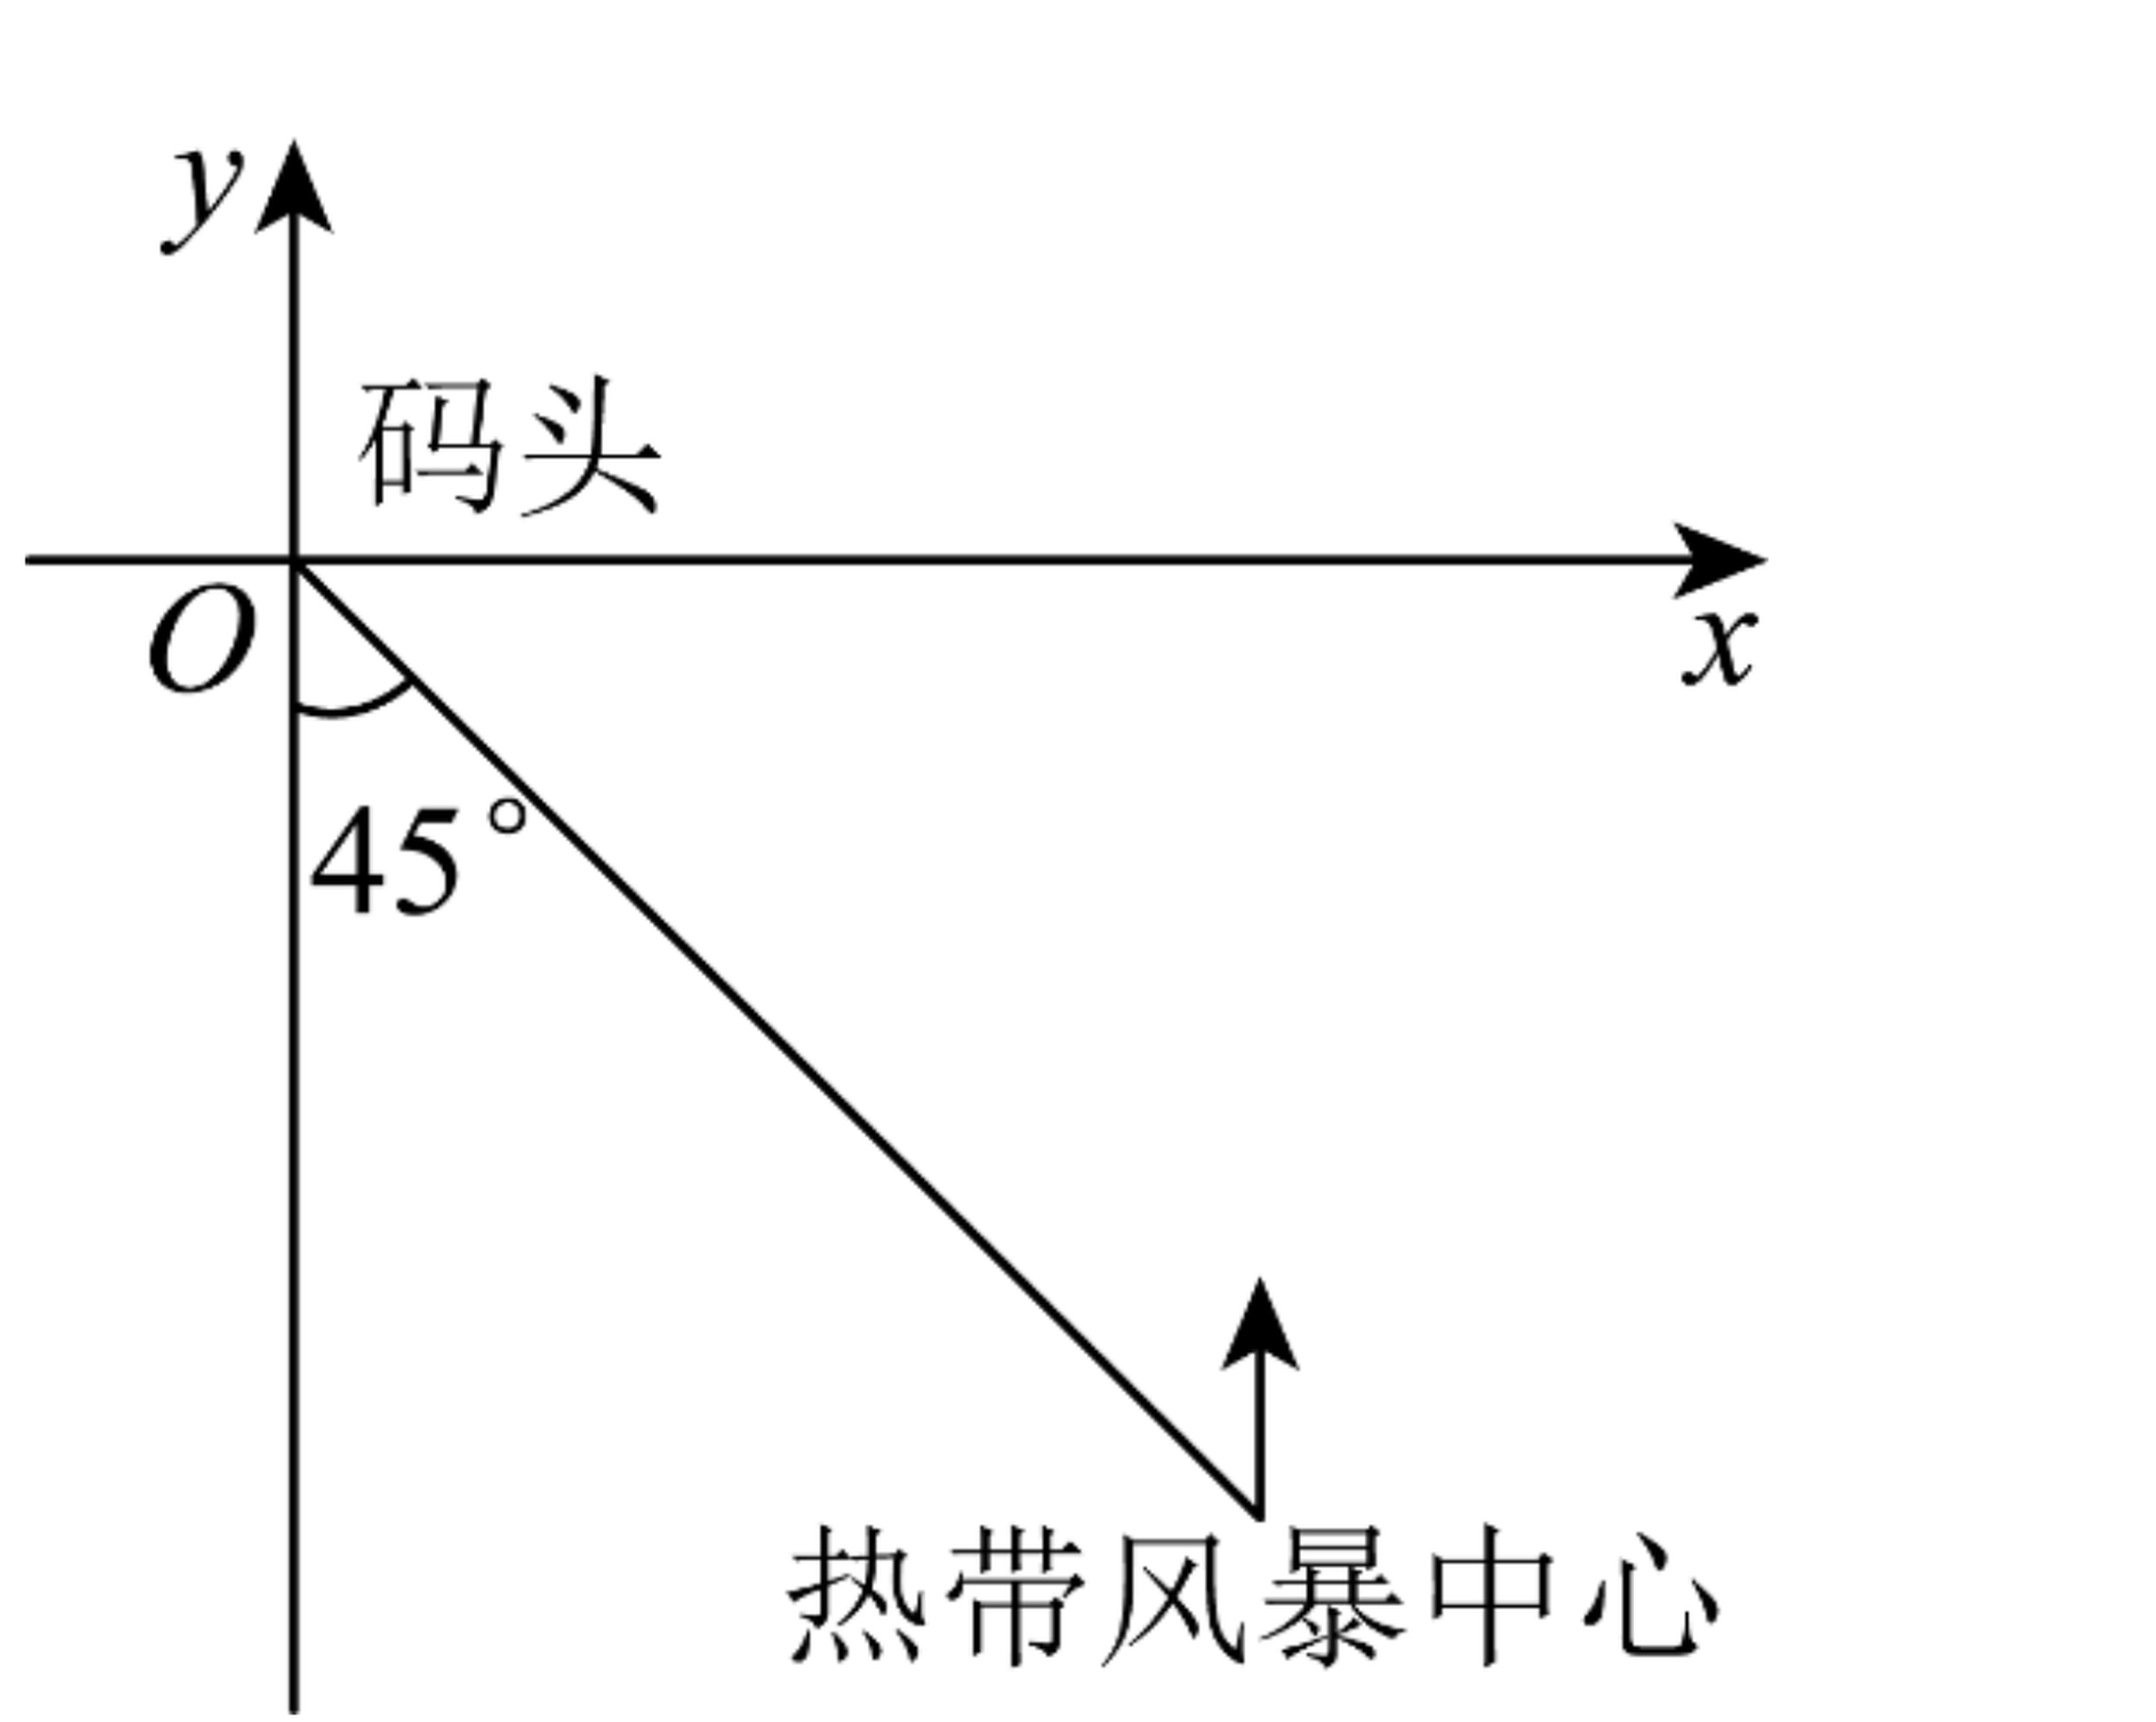
\includegraphics[width=0.36\textwidth]{figures/gao123_q5.png}
\end{center}

\ifanswer
\solbegin
\step{设风暴中心的坐标为 $(a,b)$，}
\step{由题意得 $a=400\sqrt2\times\cos45^\circ=400$，当 $a^2+b^2=400^2+b^2<500^2$，}% 原卷 $a^2$ 与 $400^2$ 并用，照录
\step{即 $-300<b<300$ 时，码头将受到风暴影响，}
\step{$\dfrac{300-(-300)}{20}=30h$，则码头受到风暴影响的时长为 30 小时，}
\step{所以由预报估计，该码头将受到热带风暴的影响时长大约为 30 小时.}
\solend
\fi

\item 已知 $a$、$b$、$c$ 为常数，若不等式 $\dfrac{ax-b}{x-c}\geqslant0$ 的解集为 $[-1,1)$，则不等式 $ax+b<0$ 的解集为\blankline[4.4em].

\ifanswer
\solbegin
\step{不等式 $\dfrac{ax-b}{x-c}\geqslant0$ 可化为 $(ax-b)(x-c)\geqslant0$ 且 $x-c\neq0$，}
\step{即 $a\left(x-\dfrac ba\right)(x-c)\geqslant0$ 且 $x\neq c$，}
\step{因为不等式 $\dfrac{ax-b}{x-c}\geqslant0$ 的解集为 $[-1,1)$，所以 $a<0$，且 $\dfrac ba=-1$,$c=1$，}
\step{即 $b=-a$，所以不等式 $ax+b<0$ 可化为 $ax-a<0$，又因为 $a<0$，所以 $x-1>0$，}
\step{解得 $x>1$，所以不等式 $ax+b<0$ 的解集为 $(1,+\infty)$.}
\solend
\fi

\item 已知实数 $a$、$b$ 满足 $ab=32$，且 $\log_2a=\log_b16$，则 $a+b$ 的值为\blankline[4.4em].

\ifanswer
\solbegin
\step{由 $\log_2a=\log_b16$，得 $\log_2a=\dfrac{\log_216}{\log_2b}$，则 $\log_2a\cdot\log_2b=4$，}
\step{由 $ab=32$，得 $\log_2a+\log_2b=\log_2ab=5$，}
\step{得 $\log_2a=1$,$\log_2b=4$ 或 $\log_2a=4$,$\log_2b=1$，}
\step{因此 $a=2$,$b=16$ 或 $a=16$,$b=2$，所以 $a+b=18$.}
\solend
\fi

\item 已知实数 $a$、$b$ 满足 $-3<a+2b<2$，$-1<2a-b<4$，则 $a+b$ 的取值范围为\blankline[4.4em].

\ifanswer
\solbegin
\step{设 $a+b=m(a+2b)+n(2a-b)=(m+2n)a+(2m-n)b$，}
\step{所以 $\begin{cases}m+2n=1\\2m-n=1\end{cases}$，解得 $n=\dfrac15$,$m=\dfrac35$，所以 $a+b=\dfrac35(a+2b)+\dfrac15(2a-b)$，}
\step{因为 $-3<(a+2b)<2$，$-1<2a-b<4$，}
\step{所以 $-\dfrac95<\dfrac35(a+2b)<\dfrac65$，$-\dfrac15<\dfrac15(2a-b)<\dfrac45$，}
\step{相加得 $-2<\dfrac35(a+2b)+\dfrac15(2a-b)<2$，即 $-2<a+b<2$，}
\step{故 $a+b$ 的取值范围为 $(-2,2)$.}
\solend
\fi

\item 存在 $x\in\R$ 使不等式 $\lvert2x-a\rvert<\lvert2a-1\rvert-2\lvert x\rvert$ 成立，则实数 $a$ 的取值范围是\blankline[4.4em].

\ifanswer
\solbegin
\step{存在 $x\in\R$，不等式 $\lvert2x-a\rvert<\lvert2a-1\rvert-2\lvert x\rvert$ 成立，}
\step{变形即 $\lvert2x-a\rvert+2\lvert x\rvert<\lvert2a-1\rvert$ 成立，}
\step{由于 $\lvert2x-a\rvert+\lvert2x\rvert\geqslant\lvert(2x-a)-2x\rvert=\lvert a\rvert$，当且仅当 $2x(2x-a)\leqslant0$ 时取等号，}
\step{因此有 $\lvert a\rvert<\lvert2a-1\rvert$，两边平方 $a^2<(2a-1)^2$，解得 $a>1$ 得 $a<\dfrac13$，}% 原卷“解得 a>1 得 a<1/3”，照录
\step{即实数 $a$ 的取值范围是 $\left(-\infty,\dfrac13\right)\cup(1,+\infty)$.}
\solend
\fi

\item 已知集合 $A=\{(x,y)\mid x^2+mx-y+2=0\}$，$B=\{(x,y)\mid x-y+1=0,0\leqslant x\leqslant3\}$，若集合 $A\cap B$ 的子集个数为 $2$，则实数 $m$ 的取值范围为\blankline[4.4em].

\ifanswer
\solbegin
\step{因为集合 $A\cap B$ 的子集个数为 $2$，所以 $A\cap B$ 的元素有一个，}
\step{即 $\begin{cases}x^2+mx-y+2=0\\x-y+1=0\end{cases}$ 在 $x\in[0,3]$ 上只有一个解，}
\step{即 $x^2+(m-1)x+1=0$ 在 $[0,3]$ 上只有一个解，}
\step{即 $1-m=x+\dfrac1x$ 在 $[0,3]$ 上只有一个解，}
\step{结合对勾函数的性质得 $1-m=2$ 或 $1-m>\dfrac{10}{3}$，解得 $m=-1$ 或 $m<-\dfrac73$.}
\solend
\fi

\item $[x]$ 表示不超过 $x$ 的最大整数，则集合 $A=\left\{y\,\middle\vert\,y=\left[\dfrac{x^2}{100}\right],x=1,2,3,\cdots,100\right\}$ 中的元素个数为\blankline[4.4em].

\ifanswer
\solbegin
\step{记 $a_k=\left[\dfrac{k^2}{100}\right](k=1,2,\cdots,100)$，$a_k$ 随 $k$ 增大而单调不减.}
\step{当 $k\geqslant50$ 时，$\dfrac{(k+1)^2}{100}-\dfrac{k^2}{100}=\dfrac{2k+1}{100}\geqslant\dfrac{101}{100}>1$，所以 $a_{k+1}\geqslant a_k+1$，}
\step{即 $a_{50}$、$a_{51}$、$\cdots$、$a_{100}$ 两两互异.}
\step{又 $a_{50}=\left[\dfrac{2500}{100}\right]=25$、$a_{100}=100$，这一段共 $100-50+1=51$ 个互异的值，}
\step{且都大于等于 $25$.}
\step{当 $k\leqslant49$ 时，$\dfrac{(k+1)^2}{100}-\dfrac{k^2}{100}=\dfrac{2k+1}{100}\leqslant\dfrac{99}{100}<1$，即 $a_k$ 每次至多增加 $1$；}
\step{又 $a_1=0$、$a_{49}=\left[\dfrac{2401}{100}\right]=24$，}
\step{故 $a_1$、$a_2$、$\cdots$、$a_{49}$ 依次取遍 $0$，$1$，$2$，$\cdots$，$24$，共 $25$ 个值.}
\step{两段取值范围互不重叠（前段不超过 $24$、后段不小于 $25$），}
\step{所以集合 $A$ 中共有 $25+51=76$ 个元素.}
\solend
\fi

\item 若实数 $a$、$b$、$c$ 满足 $\dfrac1{2^a}+\dfrac1{2^b}=1$，$\dfrac1{2^{a+b}}+\dfrac1{2^{b+c}}+\dfrac1{2^{a+c}}=1$，则 $c$ 的最大值是\blankline[4.4em].

\ifanswer
\solbegin
\step{因为 $\dfrac1{2^a}+\dfrac1{2^b}=1$，}
\step{由基本不等式得 $1=\dfrac1{2^a}+\dfrac1{2^b}\geqslant2\sqrt{\dfrac1{2^a}\cdot\dfrac1{2^b}}$（当且仅当 $a=b=1$ 时取等号），}
\step{所以 $\dfrac1{2^a}\cdot\dfrac1{2^b}\leqslant\dfrac14$，所以 $-\dfrac1{2^a}\cdot\dfrac1{2^b}\geqslant-\dfrac14$，}% 原卷带负号起论，照录
\step{因为 $\dfrac1{2^{a+b}}+\dfrac1{2^{b+c}}+\dfrac1{2^{a+c}}=1$，$\dfrac1{2^{b+c}}+\dfrac1{2^{a+c}}=\dfrac1{2^c}\left(\dfrac1{2^a}+\dfrac1{2^b}\right)=\dfrac1{2^c}$，}
\step{所以 $\dfrac1{2^c}=1-\dfrac1{2^{a+b}}\geqslant\dfrac34$，所以 $2^c\leqslant\dfrac43$，所以 $c\leqslant\log_2\dfrac43=2-\log_23$，}
\step{故 $c$ 的最大值是 $2-\log_23$.}
\solend
\fi

\end{enumerate}

\bigsec{二、选择题}

\begin{enumerate}
\setcounter{enumi}{12}

\item 下列运用等式或不等式的性质变形中，正确的是\mbox{（\quad）}

\keepwithprev
A. 如果 $a=b$，那么 $\dfrac ac=\dfrac bc$\qquad\qquad B. 如果 $\dfrac1a<\dfrac1b<0$，那么 $a-\dfrac1a>b-\dfrac1b$

C. 如果 $a>b$，那么 $\dfrac1a<\dfrac1b$\qquad\qquad D. 如果 $a>b>0$，$m\in\R$，那么 $\dfrac ba<\dfrac{b+m}{a+m}$

\ifanswer
\solbegin
\step{对于 $A$，若 $c=0$，$A$ 错误；}
\step{对于 $B$，若 $\dfrac1a<\dfrac1b<0$，则 $0>a>b$，$-\dfrac1a>-\dfrac1b>0$，}
\step{所以 $a-\dfrac1a>b-\dfrac1b$，$B$ 正确；}
\step{对于 $C$，$a>0$，$b<0$ 时，$C$ 错误；}
\step{对于 $D$，$\dfrac{b+m}{a+m}-\dfrac ba=\dfrac{ab+am}{a(a+m)}-\dfrac{ab+bm}{a(a+m)}=\dfrac{(a-b)m}{a(a+m)}$，}
\step{因为 $a>b>0$，所以 $a-b>0$，但 $m$、$a+m$ 的符号不确定，}
\step{当 $m=0$ 时，$\dfrac ba=\dfrac{b+m}{a+m}$，}
\step{当 $m(a+m)>0$ 时，$\dfrac ba<\dfrac{b+m}{a+m}$，当 $m(a+m)<0$ 时，$\dfrac ba>\dfrac{b+m}{a+m}$，$D$ 错误.}
\step{故选 $B$.}
\solend
\fi

\item “$a>b$”的一个必要非充分条件是\mbox{（\quad）}

\keepwithprev
A. $ac^2>bc^2$\qquad\quad B. $2^a>2^b$\qquad\quad C. $\left(\dfrac12\right)^{a-b}\leqslant1$\qquad\quad D. $a^3>b^3$

\ifanswer
\solbegin
\step{即“$a>b$”能推出选项，但选项不能推出“$a>b$”，故选 $C$.}
\solend
\fi

\item 若 $A=\left\{x\,\middle\vert\,x=\dfrac k6+1,k\in\Z\right\}$，$B=\left\{x\,\middle\vert\,x=\dfrac k3+\dfrac12,k\in\Z\right\}$，$C=\left\{x\,\middle\vert\,x=\dfrac{2k}{3}+\dfrac12,k\in\Z\right\}$，则这三个集合间的关系是\mbox{（\quad）}

\keepwithprev
A. $A\subseteq B\subseteq C$\qquad\quad B. $A\subseteq C\subseteq B$\qquad\quad C. $C\subseteq B\subseteq A$\qquad\quad D. $C\subseteq A\subseteq B$

\ifanswer
\solbegin
\step{若 $x\in C$，则存在 $k_0\in\Z$，使 $x=\dfrac{2k_0}{3}+\dfrac12$，}
\step{又 $2k_0\in\Z$，所以 $x\in B$，故 $C\subseteq B$，}
\step{若 $x\in B$，则存在 $k_1\in\Z$，使 $x=\dfrac{k_1}{3}+\dfrac12=\dfrac{2k_1-3}{6}+1$，}
\step{又 $2k_1-3\in\Z$，所以 $x\in A$，故 $B\subseteq A$，}
\step{又 $\dfrac43\in A$，$\dfrac43\notin B$，$\dfrac56\in B$，$\dfrac56\notin C$，所以 $C\subseteq B\subseteq A$，故选 $C$.}
\solend
\fi

\item 集合 $S=\{x\mid(x+a)(x^2+bx+c)=0\}$，$T=\{x\mid(ax+1)(cx^2+bx+1)=0\}$，其中 $a$、$b$、$c$ 为实数，若 $\lvert S\rvert$、$\lvert T\rvert$ 分别表示 $S$、$T$ 的元素个数，则下列结论中一定成立的是\mbox{（\quad）}

\keepwithprev
A. 若 $\lvert T\rvert=0$，则 $\lvert S\rvert=1$\qquad\qquad B. 若 $\lvert S\rvert=1$，则 $\lvert T\rvert=1$

C. 若 $\lvert S\rvert=2$，则 $\lvert T\rvert=2$\qquad\qquad D. 若 $\lvert T\rvert=3$，则 $\lvert S\rvert=2$

\ifanswer
\solbegin
\step{令 $f(x)=(x+a)(x^2+bx+c)$,$g(x)=(ax+1)(cx^2+bx+1)$，}
\step{对于选项 A，当 $\lvert T\rvert=0$ 时，方程 $g(x)=(ax+1)(cx^2+bx+1)=0$ 无实根，}
\step{当 $a=b=c=0$ 时，$f(x)=x^3$，由 $f(x)=0$ 得 $x=0$，此时 $\lvert S\rvert=1$；}
\step{当 $a=0$,$b^2-4c<0$ 时，$f(x)=x(x^2+bx+c)$，由 $f(x)=0$ 得 $x=0$，}
\step{此时 $\lvert S\rvert=1$，所以选项 A 正确；}
\step{对于选项 B，若 $\lvert S\rvert=1$，则 $f(x)=(x+a)(x^2+bx+c)=0$ 有且只有一根，}
\step{又 $x=-a$ 一定是 $f(x)=0$ 的根，所以 $\triangle=b^2-4c<0$，}
\step{又 $\triangle=b^2-4c<0$ 且 $a=0$ 时，$g(x)=(ax+1)(cx^2+bx+1)=0$ 无解，}
\step{此时 $\lvert T\rvert=0$，所以选项 B 错误，}
\step{对于选项 C，若 $\lvert S\rvert=2$ 时，则 $f(x)=(x+a)(x^2+bx+c)=0$ 有且只有 $2$ 根，}
\step{又 $x=-a$ 一定是 $f(x)=0$ 的根，}
\step{所以 $\triangle=b^2-4c=0$ 且 $a^2+ab+c\neq0$ 或 $\triangle=b^2-4c>0$ 且 $a^2+ab+c=0$，}
\step{当 $a=0$ 时，存在 $b$,$c$，使 $\triangle=b^2-4c=0$ 且 $a^2+ab+c\neq0$，}
\step{此时 $g(x)=(ax+1)(cx^2+bx+1)=0$ 只有一根，所以选项 C 错误，}
\step{对于选项 D，当 $\lvert T\rvert=3$ 时，方程 $g(x)=(ax+1)(cx^2+bx+1)=0$ 有三个根，}
\step{所以 $a\neq0$,$c\neq0$,$b^2-4c>0$，}
\step{设 $x_0$ 为 $g(x)=0$ 的一个根，即 $(ax_0+1)(cx_0^2+bx_0+1)=0$，}
\step{则 $x_0\neq0$，且 $f\left(\dfrac1{x_0}\right)=\left(\dfrac1{x_0}+a\right)\left(\dfrac1{x_0^2}+\dfrac1{x_0}b+c\right)=\dfrac1{x_0^3}g(x_0)=0$，}
\step{所以 $\dfrac1{x_0}$ 为方程 $f(x)=0$ 的根，故 $f(x)=0$ 有三个根，即 $\lvert T\rvert=3$ 时，}
\step{必有 $\lvert S\rvert=3$，所以选项 D 错误，}
\step{故选 $A$.}
\solend
\fi

\end{enumerate}

% 第 17 题是解答题第一题且带文氏图，守卫放在 \bigsec 之前，连节标题一起量页高
\needvspace{7cm}
\bigsec{三、解答题}

\begin{enumerate}
\setcounter{enumi}{16}

\item 设全集 $U=\R$，集合 $A=\{x\mid-2\leqslant x\leqslant4\}$，$B=\{x\mid x<-6$ 或 $x\geqslant2\}$.

（1）求图中阴影部分表示的集合；

（2）已知集合 $C=\{x\mid10-a<x<2a+1\}$，若 $\overline B\cap C=\varnothing$，求 $a$ 的取值范围.

\begin{center}
% 图取原卷截图（第 7 页题干右侧）、去水印后 2× LANCZOS 放大，本稿移至题干之后
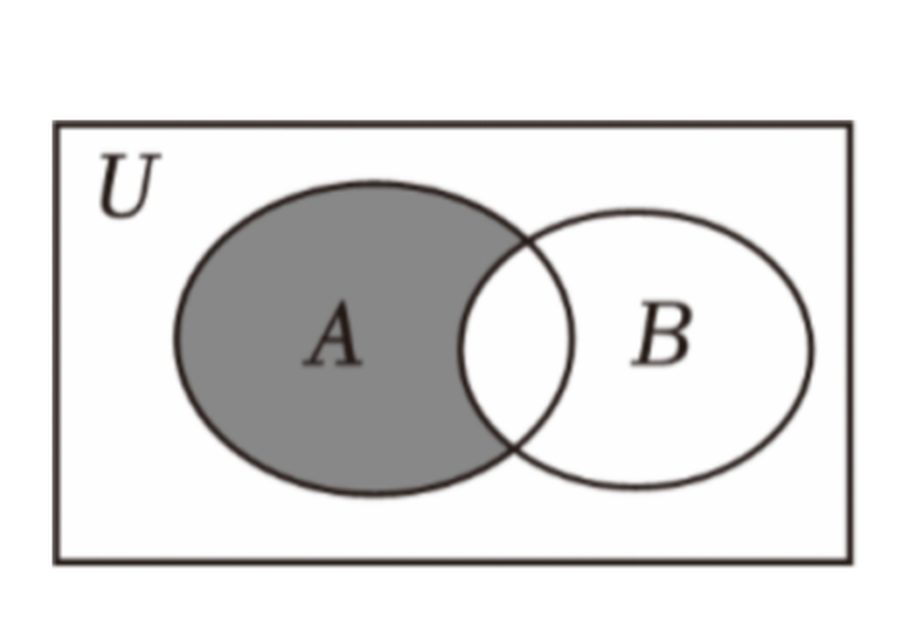
\includegraphics[width=0.34\textwidth]{figures/gao123_q17.png}
\end{center}

\ifanswer
\solbegin
\step{（1）$A\cap B=\{x\mid2\leqslant x\leqslant4\}$，}
\step{则图中阴影部分表示 $\overline{A\cap B}=\{x\mid-2\leqslant x<2\}$.}% 原卷把上划线盖在整个 $A\cap B$ 上，照录
\step{（2）由题意得 $\overline B=\{x\mid-6\leqslant x<2\}$，$C\subseteq B$，}
\step{所以当 $C=\varnothing$ 时，$10-a\geqslant2a+1$，解得 $a\leqslant3$，符合题意；}
\step{当 $C\neq\varnothing$ 时，$\begin{cases}10-a<2a+1\\2a+1\leqslant-6\end{cases}$ 或者 $\begin{cases}10-a<2a+1\\10-a\geqslant2\end{cases}$，}
\step{此时不等式组 $\begin{cases}10-a<2a+1\\2a+1\leqslant-6\end{cases}$ 无解，}
\step{不等式组 $\begin{cases}10-a<2a+1\\10-a\geqslant2\end{cases}$ 的解集为 $3<a\leqslant8$，}
\step{综上，$a$ 的取值范围为 $\{a\mid a\leqslant8\}$.}
\solend
\fi

\item (1) 求不等式：$\lvert x-1\rvert+\lvert x-2\rvert\leqslant5$ 的解集.

(2) 当 $m<1$ 时，解关于 $x$ 的不等式 $\dfrac{m(x-3)}{x+2}>1$.

\ifanswer
\solbegin
\step{(1) 当 $x<1$ 时，$\lvert x-1\rvert+\lvert x-2\rvert\leqslant5\Leftrightarrow-x+1+2-x\leqslant5$，}
\step{解得 $-1\leqslant x<1$；}
\step{当 $1\leqslant x\leqslant2$ 时，$\lvert x-1\rvert+\lvert x-2\rvert\leqslant5\Leftrightarrow x-1+2-x=1\leqslant5$ 恒成立，}
\step{所以 $1\leqslant x\leqslant2$；}
\step{当 $x>2$ 时，$\lvert x-1\rvert+\lvert x-2\rvert\leqslant5\Leftrightarrow x-1+x-2=2x-3\leqslant5$，}
\step{解得 $2<x\leqslant4$.}
\step{综上所述，不等式 $\lvert x-1\rvert+\lvert x-2\rvert\leqslant5$ 的解集为 $[-1,4]$.}
\step{(2) 原不等式变成 $\dfrac{(m-1)x-(3m+2)}{x+2}>0$，$n<1$，所以 $n-1<0$，}% 原卷作 $n<1$、$n-1<0$，与题设 $m<1$ 字母不一致，照录
\step{所以原不等式变成 $\dfrac{x-\dfrac{3m+2}{m-1}}{x+2}<0$，$\dfrac{3m+2}{m-1}-(-2)=\dfrac{5m}{m-1}$，}
\step{所以 $m<0$ 时，$\dfrac{5m}{m-1}>0$，$\dfrac{3m+2}{m-1}>-2$，}
\step{原不等式的解集为 $\left(-2,\dfrac{3m+2}{m-1}\right)$；}
\step{$m=0$ 时，原不等式变成 $1<0$，无解；}
\step{$0<m<1$ 时，$\dfrac{5m}{m-1}<0$，$\dfrac{3m+2}{m-1}<-2$，}
\step{原不等式的解集为 $\left(\dfrac{3m+2}{m-1},-2\right)$.}
\solend
\fi

\item 在园林博览会上，某公司带来了一种智能设备供采购商洽谈采购，并决定大量投放市场，已知该种设备年固定研发成本为 $50$ 万元，每生产一台需另投入 $100$ 元，设该公司一年内生产该设备 $x$ 万台且全部售完，每万台的销售收入 $G(x)$（万元）与年产量 $x$（万台）满足如下关系式：$G(x)=\begin{cases}180-x,0<x\leqslant20\\80+\dfrac{2000}{x}-\dfrac{8000}{x(x-1)},x>20\end{cases}$.

(1) 写出年利润 $W(x)$（万元）关于年产量 $x$（万台）的函数解析式；（利润 $=$ 销售收入 $-$ 成本）

(2) 当年产量为多少万台时，该公司获得的年利润最大，并求出最大利润.

\ifanswer
\solbegin
\step{(1) $W(x)=xG(x)-50-100x=\begin{cases}-50+80x-x^2,0<x\leqslant20\\-20x+1950-\dfrac{8000}{x-1},x>20\end{cases}$；}
\step{(2) 当 $0<x\leqslant20$ 时，$W(x)=-50+80x-x^2=-(x-40)^2+1550$，}
\step{由函数性质得当 $x\leqslant40$ 时严格增，所以当 $x=20$ 时，$W(x)_{max}=1150$，}
\step{当 $x>20$ 时，$W(x)=-20x+1950-\dfrac{8000}{x-1}=-20\left[(x-1)+\dfrac{400}{x-1}\right]+1930$，}
\step{$W(x)=-20\left[(x-1)+\dfrac{400}{x-1}\right]+1930\leqslant-20\times2\sqrt{(x-1)\cdot\dfrac{400}{x-1}}+1930$}
\step{$=1130$，当且仅当 $x-1=\dfrac{400}{x-1}$，即 $x=21$ 时取等号，}
\step{所以 $W(x)_{max}=1130$，}
\step{因为 $1150>1130$，所以当 $x=20$ 时，$W(x)_{max}=1150$，}
\step{即当年产量为 $20$ 万台时，该公司获得的年利润最大，}
\step{最大利润为 $1150$ 万元.}
\solend
\fi

\item 关于 $x$ 的方程 $(x^2-1)^2-2k\lvert x^2-1\rvert+k+1=0(k\in\R)$.

(1) 若方程无实根，求 $k$ 的取值范围；

(2) 若方程有 $4$ 个不等实根，求 $k$ 的取值范围；

(3) 若 $k=a+b$，且满足 $\dfrac1{a+2b}+\dfrac1{a+3}=\dfrac12$，$a>0$，$b>0$，试判断方程根的个数.

\ifanswer
\solbegin
\step{(1) 关于 $x$ 的方程 $(x^2-1)^2-2k\lvert x^2-1\rvert+k+1=0(k\in\R)$，}
\step{令 $t=\lvert x^2-1\rvert$，则 $t\geqslant0$，则原方程转化为 $t^2-2kt+k+1=0(*)$，}
\step{因为关于 $x$ 的方程 $(x^2-1)^2-2k\lvert x^2-1\rvert+k+1=0(k\in\R)$ 无实根，}
\step{所以 $(*)$ 式无实根或实根均小于零，令 $f(t)=t^2-2kt+k+1$，}
\step{①若 $(*)$ 式无实根，则 $\triangle<0$，解得 $\dfrac{1-\sqrt5}{2}<k<\dfrac{1+\sqrt5}{2}$，}
\step{②两根均为负，则 $\begin{cases}\Delta\geqslant0\\t_{\text{对}}=k<0\\f(0)>0\end{cases}$，解得 $-1<k\leqslant\dfrac{1-\sqrt5}{2}$，}
\step{综合①②，得 $k$ 的取值范围是 $\left(-1,\dfrac{1+\sqrt5}{2}\right)$；}
\step{(2) 作函数 $t=\lvert x^2-1\rvert$ 的图象，}
\begin{center}
% 图取原卷截图（第 11 页解析内）、去水印后 2× LANCZOS 放大，仅答案版出
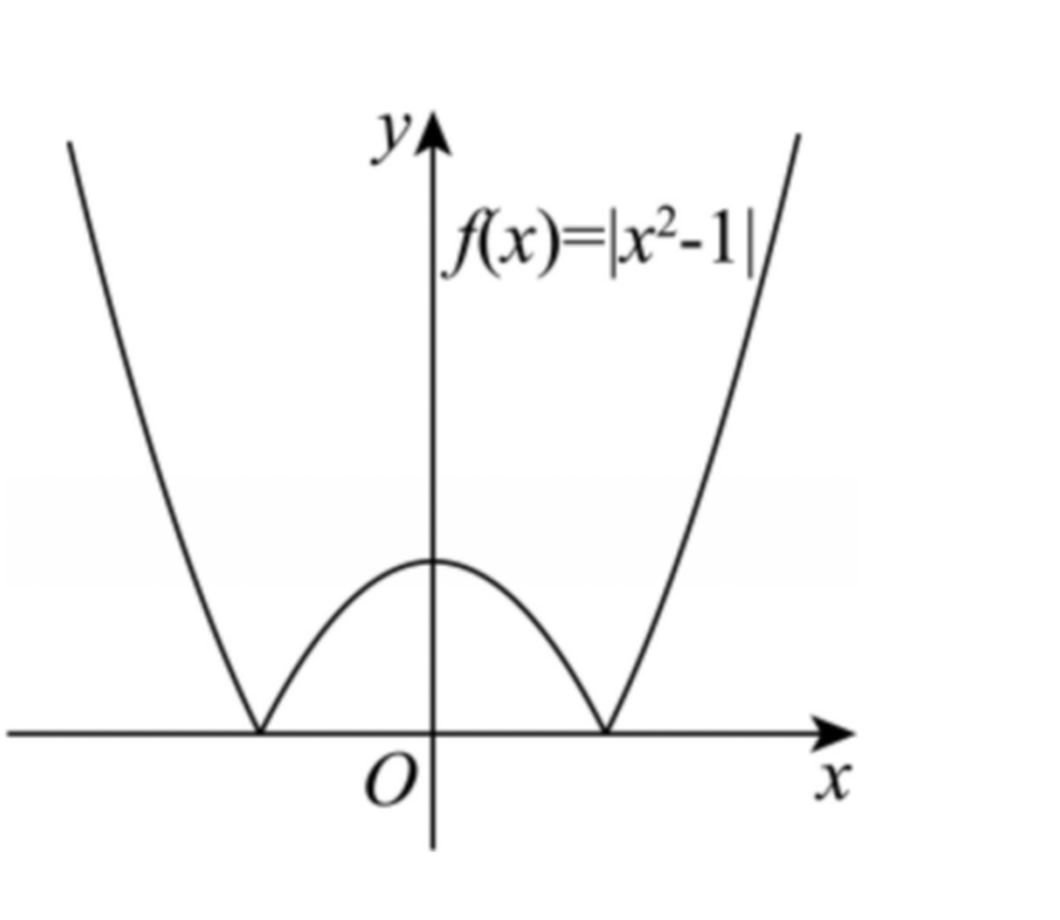
\includegraphics[width=0.40\textwidth]{figures/gao123_q20.png}
\end{center}
\step{$t=0$ 或 $t>1$ 时，每一个 $t$ 值对应 $2$ 个不同的 $x$ 值，}
\step{$t=1$ 时一个 $t$ 值对应 $3$ 个不同的 $x$ 值，}
\step{$0<t<1$ 时一个 $t$ 值对应 $4$ 个不同的 $x$ 值，}
\step{要使原方程有四个不等实根，}
\step{①$(*)$ 式一根为零，另一根大于 $1$，无解；}
\step{②$(*)$ 有两不等根且两根均大于 $1$，则 $\begin{cases}\Delta>0\\t_{\text{对}}=k>1\\f(1)>0\end{cases}$，解得 $\dfrac{1+\sqrt5}{2}<k<2$；}
\step{④$(*)$ 式有 $1$ 实根在 $(0,1)$ 之间，另一根小于零，}% 原卷由 ② 直接跳到 ④，缺 ③，照录
\step{则 $\begin{cases}f(0)<0\\f(1)>0\end{cases}$，所以 $\begin{cases}k+1<0\\2-k>0\end{cases}$，解得 $k<-1$，}
\step{综上所述，$k$ 取值范围为 $(-\infty,-1)\cup\left(\dfrac{1+\sqrt5}{2},2\right)$；}
\step{(3) 因为 $\dfrac1{a+2b}+\dfrac1{a+3}=\dfrac{a+2b+a+3}{(a+2b)(a+3)}=\dfrac{2(a+b)+3}{(a+2b)(a+3)}=\dfrac12$，}
\step{所以 $2(a+b)+3=\dfrac12(a+2b)(a+3)$，}
\step{因为 $a$、$b$ 为正实数，所以 $\dfrac12=\dfrac1{a+2b}+\dfrac1{a+3}\geqslant2\sqrt{\dfrac1{a+2b}\times\dfrac1{a+3}}$，}
\step{得 $\dfrac1{16}\geqslant\dfrac1{a+2b}\times\dfrac1{a+3}$，即 $(a+2b)(a+3)\geqslant16$，}
\step{所以 $2(a+b)+3\geqslant8$，即 $a+b\geqslant\dfrac52$，}
\step{当且仅当 $\dfrac1{a+2b}=\dfrac1{a+3}$ 即 $a=1$,$b=\dfrac32$ 时取等号，}
\step{故 $k\geqslant\dfrac52$，此时有 $\begin{cases}\Delta>0\\t_{\text{对}}=k>1\\f(0)>0,f(1)<0\end{cases}$，}
\step{故 $(*)$ 式有两不等实根且一根在 $(0,1)$ 之间，另一根大于 $1$，}
\step{故原方程有 $6$ 个实根.}
\solend
\fi

\item 设 $n$ 是不小于 $3$ 的正整数，集合 $S_n=\{(a_1,a_2,\cdots,a_n)\mid a_i\in\{0,1\},i=1,2,\cdots,n\}$，对于集合 $S_n$ 中任意两个元素 $A=(a_1,a_2,\cdots,a_n)$，$B=(b_1,b_2,\cdots,b_n)$.

定义 1：$A\cdot B=n-(\lvert a_1-b_1\rvert+\lvert a_2-b_2\rvert+\cdots+\lvert a_n-b_n\rvert)$，

定义 2：若 $A\cdot B=0$，则称互为相反元素，记作 $A=\overline B$ 或 $B=\overline A$.

(1) 若 $n=3$，$A=(0,1,0)$，$B=(1,1,0)$，试写出 $\overline A$、$\overline B$ 以及 $A\cdot B$ 的值；

(2) 若 $A$、$B\in S_n$，$A=(a_1,a_2,\cdots,a_n)$，$B=(b_1,b_2,\cdots,b_n)$，证明：$A\cdot B+\overline A\cdot B=n$；

(3) 设 $k$ 是小于 $n$ 的正奇数，至少含有两个元素的集合 $M\subseteq S_n$，且对于集合 $M$ 中任意两个不相同的元素 $A=(a_1,a_2,\cdots,a_n)$，$B=(b_1,b_2,\cdots,b_n)$，都有 $A\cdot B=n-k$，试求集合 $M$ 中元素个数的所有可能值.

\ifanswer
\solbegin
\step{(1) $\overline A=(1,0,1)$,$\overline B=(0,0,1)$,$\overline A\cdot\overline B=2$；}
\step{(2) 设 $A=(a_1,a_2,\cdots,a_n)$,$B=(b_1,b_2,\cdots,b_n)$,$\overline A=(x_1,x_2,\cdots,x_n)$，}
\step{由 $a_i$、$b_i$、$x_i\in\{0,1\}$，$i=1,2,\cdots,n$，得 $\lvert a_i-x_i\rvert\leqslant1$，$i=1,2,\cdots,n$，}
\step{所以 $\lvert a_1-x_1\rvert+\lvert a_2-x_2\rvert+\cdots+\lvert a_i-x_i\rvert\leqslant n$，}% 原卷末项下标作 $i$，照录
\step{当且仅当 $\lvert a_i-x_i\rvert=1$，$i=1,2,\cdots,n$，}
\step{即 $x_i=1-a_i$，$i=1,2,\cdots,n$ 时取等号.}
\step{由题意得 $A\cdot\overline A=n-(\lvert a_1-x_1\rvert+\lvert a_2-x_2\rvert+\cdots+\lvert a_n-x_n\rvert)=0$，}
\step{即 $\lvert a_1-x_1\rvert+\lvert a_2-x_2\rvert+\cdots+\lvert a_n-x_n\rvert=n$，}
\step{所以 $x_i=1-a_i$，$i=1,2,\cdots,n$，}
\step{$A\cdot B+\overline A\cdot B=2n-\sum\limits_{i=1}^n[\lvert a_i-b_i\rvert+(1-a_i)-b_i]$}
\step{$=2n-\sum\limits_{i=1}^n(\lvert1-b_i\rvert+\lvert0-b_i\rvert)=2n-\sum\limits_{i=1}^n(1-b_i+b_i)=2n-n=n$；}
\step{(3) 假设 $A=(a_1,a_2,\cdots,a_n)$，$B=(b_1,b_2,\cdots,b_n)$，$C=(c_1,c_2,\cdots,c_n)$}
\step{为集合 $M$ 中的三个不相同的元素，}
\step{则 $A\cdot B=n-(\lvert a_1-b_1\rvert+\lvert a_2-b_2\rvert+\cdots+\lvert a_n-b_n\rvert)=n-k$，}
\step{即 $\lvert a_1-b_1\rvert+\lvert a_2-b_2\rvert+\cdots+\lvert a_n-b_n\rvert=k$，}
\step{又由题意得 $\lvert a_i-b_i\rvert=0$ 或 $1$，$i=1,2,\cdots,n$，}
\step{$\lvert a_1-b_1\rvert$、$\lvert a_2-b_2\rvert$、$\cdots$、$\lvert a_n-b_n\rvert$ 恰有 $k$ 个 $1$，$n-k$ 个 $0$，}
\step{设其中 $k$ 个等于 $1$ 的项以此为 $a_{m_1}-b_{m_1}$,$a_{m_2}-b_{m_2}$,$\cdots$,$a_{m_k}-b_{m_k}$，}
\step{$n-k$ 个等于 $0$ 的项为 $a_{m_{k+1}}-b_{m_{k+1}}$,$a_{m_{k+2}}-b_{m_{k+2}}$,$\cdots$,$a_{m_n}-b_{m_n}$，}
\step{由题意得 $A\cdot C=n-(\lvert a_1-c_1\rvert+\lvert a_2-c_2\rvert+\cdots+\lvert a_n-c_n\rvert)=n-k$，}
\step{所以 $\sum\limits_{i=1}^k\lvert a_{m_i}-c_{m_i}\rvert+\sum\limits_{j=k+1}^n\lvert a_{m_j}-c_{m_j}\rvert=k$ ①，}
\step{同理 $\sum\limits_{i=1}^k\lvert b_{m_i}-c_{m_i}\rvert+\sum\limits_{j=k+1}^n\lvert b_{m_j}-c_{m_j}\rvert=k$ ②，}
\step{因为 $\lvert a_{m_{k+1}}-b_{m_{k+1}}\rvert=\lvert a_{m_{k+2}}-b_{m_{k+2}}\rvert=\cdots=\lvert a_{m_n}-b_{m_n}\rvert=0$，}
\step{所以 $\sum\limits_{j=k+1}^n\lvert a_{m_j}-c_{m_j}\rvert=\sum\limits_{j=k+1}^n\lvert b_{m_j}-c_{m_j}\rvert$，}
\step{由①$-$②得 $\sum\limits_{i=1}^k(\lvert a_{m_i}-c_{m_i}\rvert-\lvert b_{m_i}-c_{m_i}\rvert)=0$，}
\step{又 $\sum\limits_{i=1}^k(\lvert a_{m_i}-c_{m_i}\rvert-\lvert b_{m_i}-c_{m_i}\rvert)=\sum\limits_{i=1}^k(\lvert1-c_{m_i}\rvert-\lvert0-c_{m_i}\rvert)=k-2\sum\limits_{i=1}^k c_{m_i}$}
\step{为奇数，与 $\sum\limits_{i=1}^k(\lvert a_{m_i}-c_{m_i}\rvert-\lvert b_{m_i}-c_{m_i}\rvert)=0$ 矛盾，所以假设不成立，}
\step{即集合 $M$ 中至多有两个元素，}
\step{当 $M=\{(1,1,\cdots,1,0,0,\cdots,0),(0,0,\cdots,0)\}$ 时符合题意，}
\step{所以集合 $M$ 中元素的个数只可能是 $2$.}
\solend
\fi

\end{enumerate}

\end{document}
"
% 紧凑版：xelatex "\def\iscompact{1}% 高一123_行知中学_10月月考.tex
%   —— 高一上数学“2026-2027 年行知中学高一上 10 月月考”（试卷版/答案版）
% 试卷版：xelatex 高一123_行知中学_10月月考.tex
% 答案版：xelatex "\def\isanswer{1}% 高一123_行知中学_10月月考.tex
%   —— 高一上数学“2026-2027 年行知中学高一上 10 月月考”（试卷版/答案版）
% 试卷版：xelatex 高一123_行知中学_10月月考.tex
% 答案版：xelatex "\def\isanswer{1}\input{高一123_行知中学_10月月考.tex}"
% 紧凑版：xelatex "\def\iscompact{1}\input{高一123_行知中学_10月月考.tex}"
%
% 原始材料：微信公众号“魔都数学加油站”文章，作者破晓，2026-11-09 17:52 发布；
% 连载“27学年高一123”，原文标题“27学年高一123——2026-2027年上海市行知中学高一上10月月考”；
% 原文链接：https://mp.weixin.qq.com/s/GV4SWBLUJrBhMQwo22FVzg。
% 正文为 14 张 PNG 页（第 7、9、11、13、14 页 2560×3620，其余 4762×6735），
% 题目下印有【答案】或【解析】，为讲评版。
% 题目、解析均据原图转录；卷面红色水印及公众号页脚未录入。
% 全卷 3 张插图：第 5 题的坐标示意图、第 17 题的文氏图（均属题干，三版都出）、
% 第 20 题 (2) 的 $t=\lvert x^2-1\rvert$ 图象（属解析，仅答案版出）；
% 都取原卷截图去水印、2× LANCZOS 放大，见 figures/gao123_q5.png、
% figures/gao123_q17.png、figures/gao123_q20.png。
%
% 卷首标题：原卷印作“2026-2027 年行知中学高一上 10 月月考”（公众号标题中的“上海市”
% 卷面标题行没有，本稿照卷面），年份区间按全稿惯例排 en dash；原卷未印副标题，本稿按题目内容
% 标为“集合与常用逻辑用语、不等式”（与 110／111／113／116／118／120 同）。
%
% 与原卷的排版差异：
%   ① 原文从第 3 题起，填空题编号为 3—12、选择题为 13—16、解答题为 17—21，本稿保留原题号；
%   ② 原卷每题下直接印【解析】／【答案】，本稿按全稿惯例置于答案版；第 3 题只印【答案】、
%      另提 \ans{}；选择题答案在解析末句“故选 …”，括号内留空；
%   ③ 原卷未印副标题，本稿按“知识模块”口径补出；
%   ④ 原卷填空横线按全稿惯例排为 \blankline[4.4em]；选择题括号排 \mbox{（\quad）}、
%      选项段前按惯例加 \keepwithprev；解答题不留作答区（原卷为讲评版，与 109—122 同）；
%   ⑤ 原卷数集排斜体 $R$／$Z$（第 9 题作粗体 $\mathbf{R}$），按全稿惯例改 \R／\Z；
%      绝对值按全稿惯例排 \lvert…\rvert，集合描述竖线排 \mid；单位 km、h 原卷排斜体，
%      本稿按正体照排；补集照原卷上划线排 \overline{B}、\overline{A}。
%
% 判别式与子集符号：第 16 题解析的 $\triangle=b^2-4c<0$、第 20 题 (1) ① 的 $\triangle<0$
%   均作等边、扁的 \triangle；第 20 题 ② 两处 cases 与 (3) 的 $\Delta\geqslant0$／$\Delta>0$
%   作等腰、高的 \Delta，逐处照录、不统一；第 15 题选项与第 17 题 (2) 的 $\subseteq$
%   印有下划线，照录 \subseteq。
%
% 原卷存疑照录：
%   第 4 题解析“若 $-\lvert a\rvert=0$，则 $a=0$，则 $A=\{0,-1,0\}$”以元素重复说明互异性；
%   第 5 题解析“当 $a^2+b^2=400^2+b^2<500^2$”等式左边 $a^2$ 与 $400^2$ 并用；
%   第 9 题解析“解得 $a>1$ 得 $a<\dfrac13$”（按平方不等式应为 $a>1$ 或 $a<\dfrac13$）；
%   第 12 题解析“所以 $-\dfrac1{2^a}\cdot\dfrac1{2^b}\geqslant-\dfrac14$”带负号起论；
%   第 17 题 (1) 解析把阴影部分（实为 $A\cap\overline B$）印作 $\overline{A\cap B}$；
%   第 18 题 (2) 解析作“$n<1$，所以 $n-1<0$”，与题设 $m<1$ 字母不一致；
%   第 20 题 (2) 的情形编号由 ①、② 直接跳到 ④（缺 ③）；
%   第 21 题 (2) 解析“$\lvert a_1-x_1\rvert+\cdots+\lvert a_i-x_i\rvert\leqslant n$”
%   末项下标作 $i$（按上下文应为 $n$）。以上均照录加注。
%
% 行数核对：逐题数 \step 条数，合计 176 条（Q3：0；Q4：6；Q5：5；Q6：5；Q7：4；
% Q8：6；Q9：5；Q10：5；Q11：10；Q12：6；Q13：9；Q14：1；Q15：5；Q16：21；
% Q17：8；Q18：14；Q19：10；Q20：26；Q21：30），与原卷印刷行逐题相等
% （cases 块作一个印刷行计）。第 3 题只印【答案】，提 \ans{}，不计入 \step 账。
%
\documentclass[a4paper,11pt]{article}
\usepackage{common}

\begin{document}

\examtitlest[3]{2026--2027 年行知中学高一上 10 月月考}{集合与常用逻辑用语、不等式}

\bigsec{一、填空题}

\begin{enumerate}
\setcounter{enumi}{2}

\item 写出命题“存在实数 $x$、$y$、$z$，使 $x<y$ 或 $y<z$.”的否定\blankline[4.4em].

\ifanswer
\ans{任意实数 $x$、$y$、$z$，使得 $x\geqslant y$ 且 $y\geqslant z$}
\fi

\item 若集合 $\{0,-1,2a\}=\{a-1,-\lvert a\rvert,a+1\}$，实数 $a$ 的值为\blankline[4.4em].

\ifanswer
\solbegin
\step{令 $A=\{0,-1,2a\}$,$B=\{a-1,-\lvert a\rvert,a+1\}$，}
\step{因为 $\{0,-1,2a\}=\{a-1,-\lvert a\rvert,a+1\}$，}
\step{若 $a-1=0$，则 $a=1$，则 $A=\{0,-1,2\}$,$B=\{0,-1,2\}$，满足要求；}
\step{若 $-\lvert a\rvert=0$，则 $a=0$，则 $A=\{0,-1,0\}$，不满足集合元素的互异性；}% 原卷以 $A=\{0,-1,0\}$ 说明互异性，照录
\step{若 $a+1=0$，则 $a=-1$，则 $A=\{0,-1,-2\}$,$B=\{0,-1,-2\}$，满足要求；}
\step{故实数 $a$ 的值为 $\pm1$.}
\solend
\fi

\needvspace{7cm}
\item 如图，据气象部门预报，在距离某码头南偏东 $45^\circ$ 方向 $400\sqrt2$ km 处的热带
风暴中心正在以 $20$km/h 的速度向正北方向移动，距风暴中心 $500$km 以内
的地区都将受到影响. 以上预报估计，该码头将受到热带风暴的影响时长大
约为\blankline[4.4em]$h$.

\begin{center}
% 图取原卷截图（第 1 页题干右侧）、去水印后 2× LANCZOS 放大，本稿移至题干之后
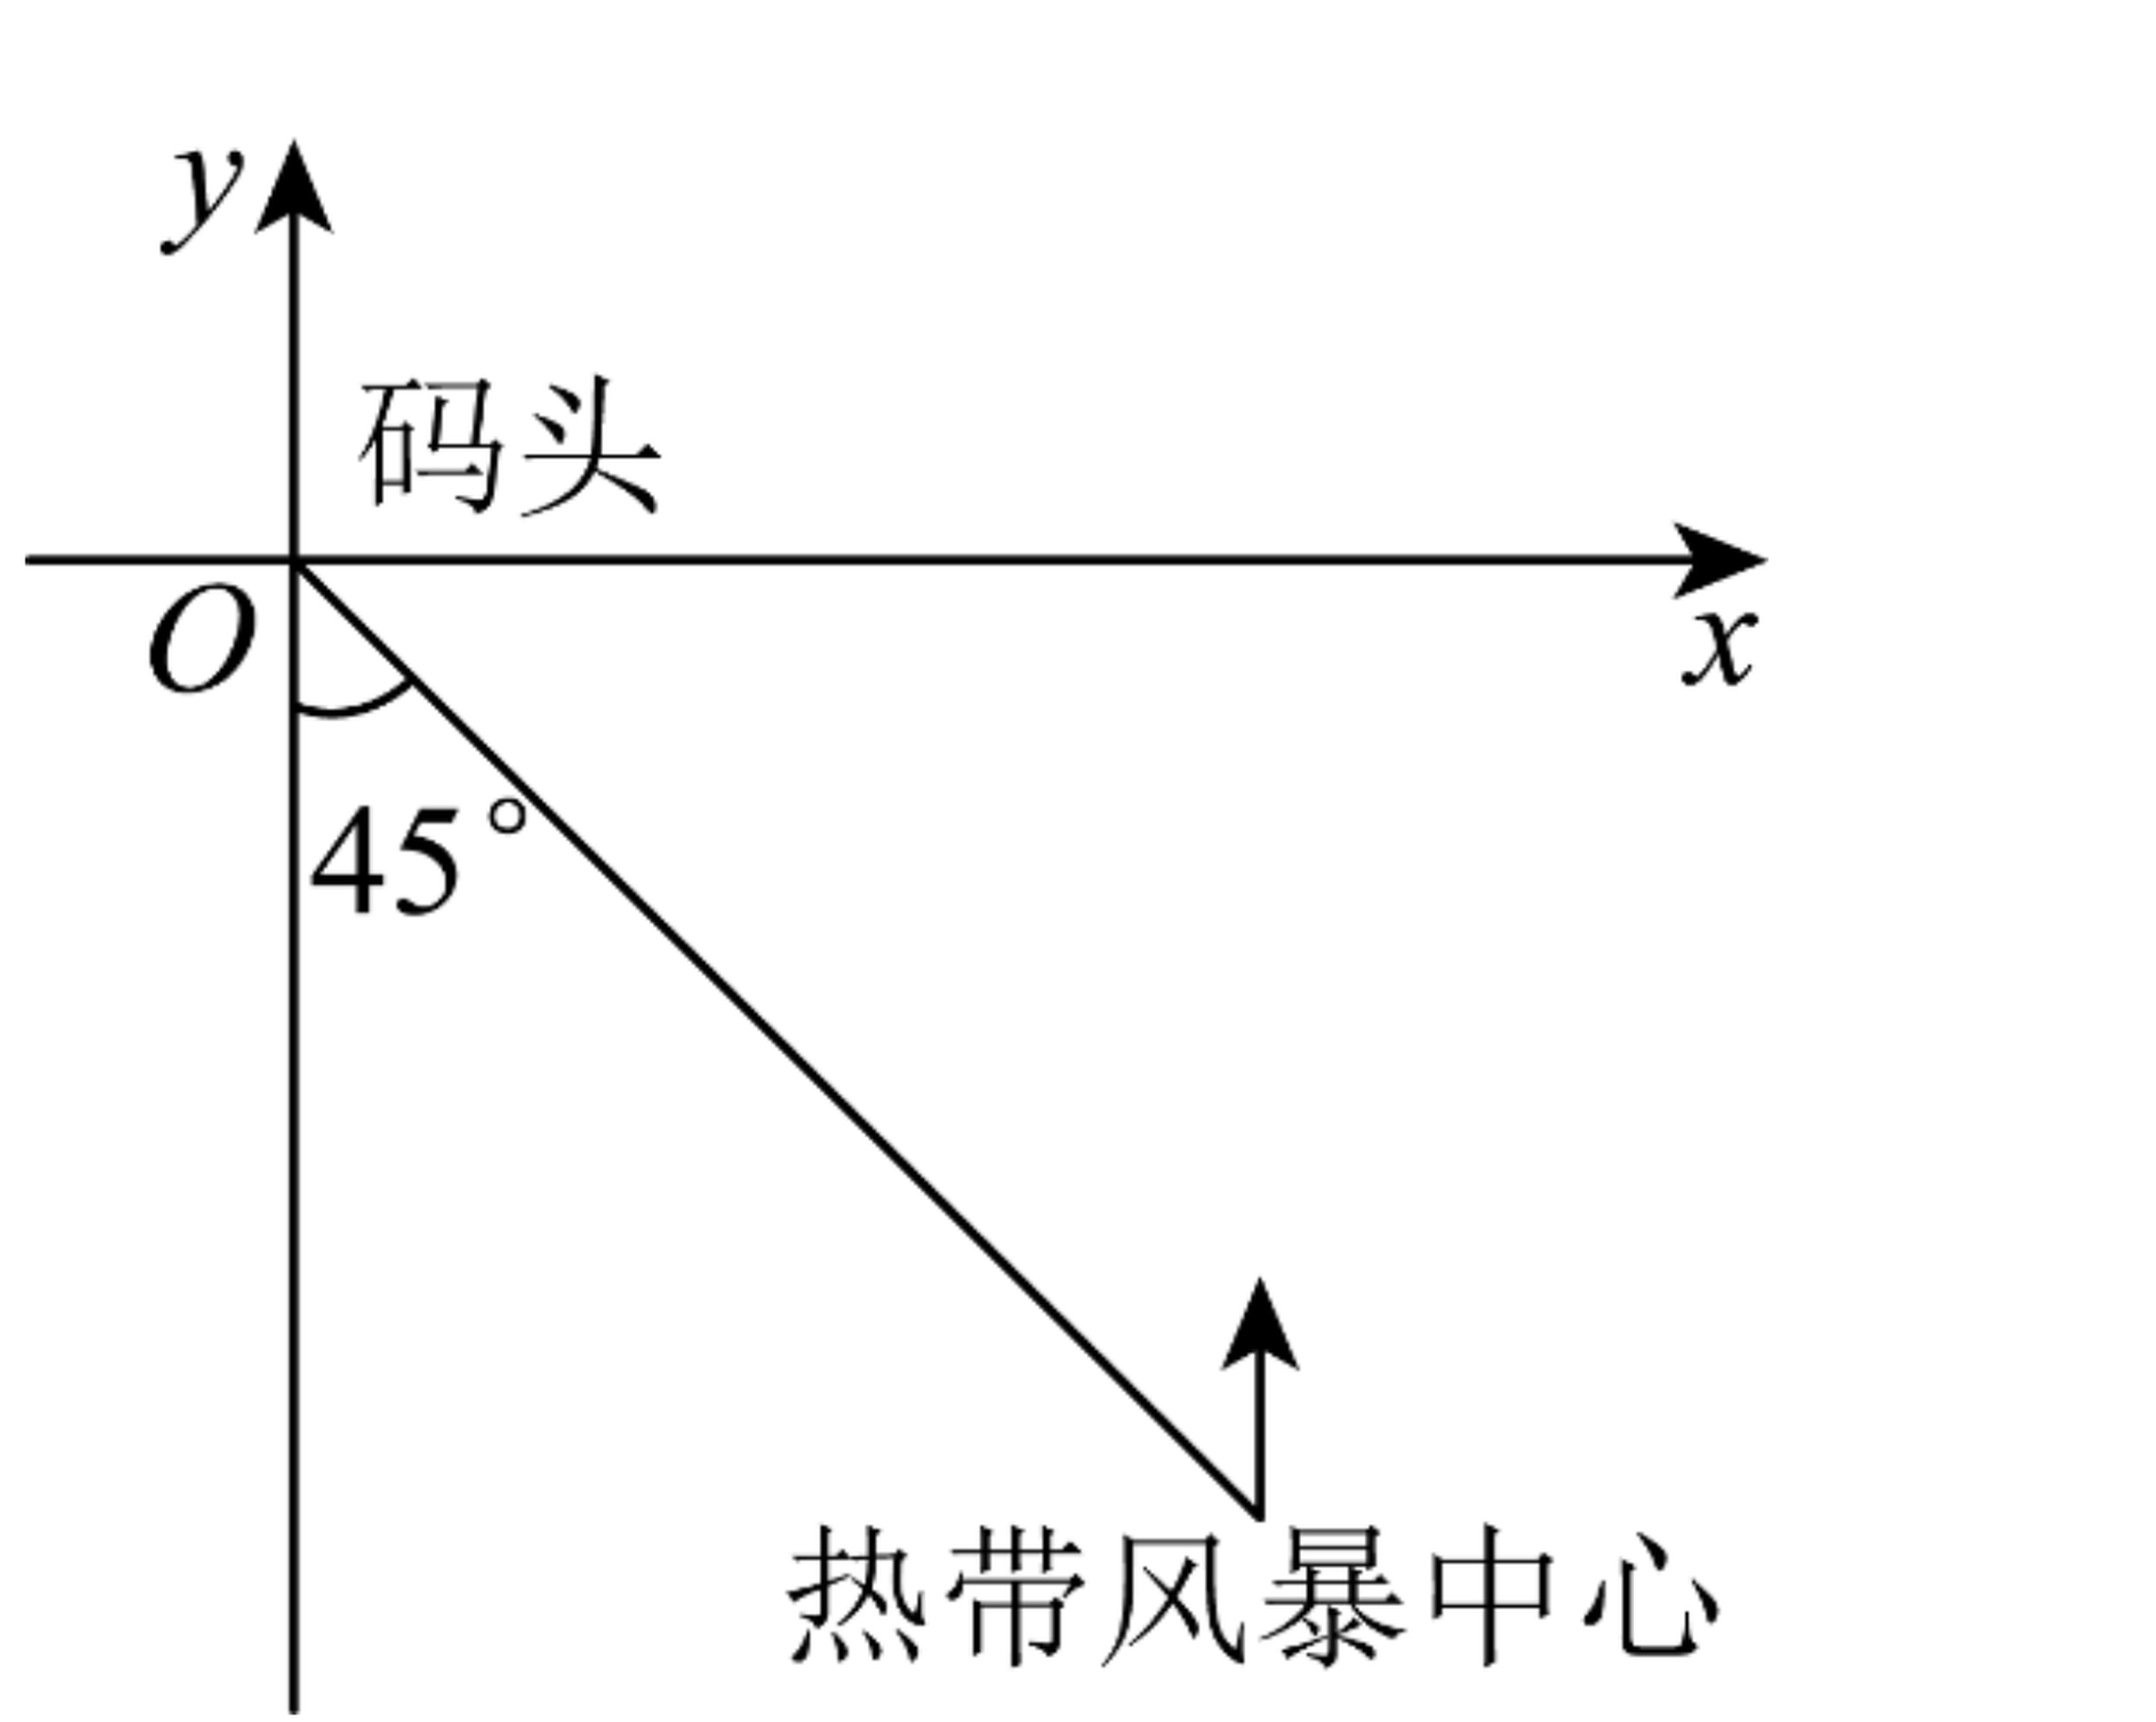
\includegraphics[width=0.36\textwidth]{figures/gao123_q5.png}
\end{center}

\ifanswer
\solbegin
\step{设风暴中心的坐标为 $(a,b)$，}
\step{由题意得 $a=400\sqrt2\times\cos45^\circ=400$，当 $a^2+b^2=400^2+b^2<500^2$，}% 原卷 $a^2$ 与 $400^2$ 并用，照录
\step{即 $-300<b<300$ 时，码头将受到风暴影响，}
\step{$\dfrac{300-(-300)}{20}=30h$，则码头受到风暴影响的时长为 30 小时，}
\step{所以由预报估计，该码头将受到热带风暴的影响时长大约为 30 小时.}
\solend
\fi

\item 已知 $a$、$b$、$c$ 为常数，若不等式 $\dfrac{ax-b}{x-c}\geqslant0$ 的解集为 $[-1,1)$，则不等式 $ax+b<0$ 的解集为\blankline[4.4em].

\ifanswer
\solbegin
\step{不等式 $\dfrac{ax-b}{x-c}\geqslant0$ 可化为 $(ax-b)(x-c)\geqslant0$ 且 $x-c\neq0$，}
\step{即 $a\left(x-\dfrac ba\right)(x-c)\geqslant0$ 且 $x\neq c$，}
\step{因为不等式 $\dfrac{ax-b}{x-c}\geqslant0$ 的解集为 $[-1,1)$，所以 $a<0$，且 $\dfrac ba=-1$,$c=1$，}
\step{即 $b=-a$，所以不等式 $ax+b<0$ 可化为 $ax-a<0$，又因为 $a<0$，所以 $x-1>0$，}
\step{解得 $x>1$，所以不等式 $ax+b<0$ 的解集为 $(1,+\infty)$.}
\solend
\fi

\item 已知实数 $a$、$b$ 满足 $ab=32$，且 $\log_2a=\log_b16$，则 $a+b$ 的值为\blankline[4.4em].

\ifanswer
\solbegin
\step{由 $\log_2a=\log_b16$，得 $\log_2a=\dfrac{\log_216}{\log_2b}$，则 $\log_2a\cdot\log_2b=4$，}
\step{由 $ab=32$，得 $\log_2a+\log_2b=\log_2ab=5$，}
\step{得 $\log_2a=1$,$\log_2b=4$ 或 $\log_2a=4$,$\log_2b=1$，}
\step{因此 $a=2$,$b=16$ 或 $a=16$,$b=2$，所以 $a+b=18$.}
\solend
\fi

\item 已知实数 $a$、$b$ 满足 $-3<a+2b<2$，$-1<2a-b<4$，则 $a+b$ 的取值范围为\blankline[4.4em].

\ifanswer
\solbegin
\step{设 $a+b=m(a+2b)+n(2a-b)=(m+2n)a+(2m-n)b$，}
\step{所以 $\begin{cases}m+2n=1\\2m-n=1\end{cases}$，解得 $n=\dfrac15$,$m=\dfrac35$，所以 $a+b=\dfrac35(a+2b)+\dfrac15(2a-b)$，}
\step{因为 $-3<(a+2b)<2$，$-1<2a-b<4$，}
\step{所以 $-\dfrac95<\dfrac35(a+2b)<\dfrac65$，$-\dfrac15<\dfrac15(2a-b)<\dfrac45$，}
\step{相加得 $-2<\dfrac35(a+2b)+\dfrac15(2a-b)<2$，即 $-2<a+b<2$，}
\step{故 $a+b$ 的取值范围为 $(-2,2)$.}
\solend
\fi

\item 存在 $x\in\R$ 使不等式 $\lvert2x-a\rvert<\lvert2a-1\rvert-2\lvert x\rvert$ 成立，则实数 $a$ 的取值范围是\blankline[4.4em].

\ifanswer
\solbegin
\step{存在 $x\in\R$，不等式 $\lvert2x-a\rvert<\lvert2a-1\rvert-2\lvert x\rvert$ 成立，}
\step{变形即 $\lvert2x-a\rvert+2\lvert x\rvert<\lvert2a-1\rvert$ 成立，}
\step{由于 $\lvert2x-a\rvert+\lvert2x\rvert\geqslant\lvert(2x-a)-2x\rvert=\lvert a\rvert$，当且仅当 $2x(2x-a)\leqslant0$ 时取等号，}
\step{因此有 $\lvert a\rvert<\lvert2a-1\rvert$，两边平方 $a^2<(2a-1)^2$，解得 $a>1$ 得 $a<\dfrac13$，}% 原卷“解得 a>1 得 a<1/3”，照录
\step{即实数 $a$ 的取值范围是 $\left(-\infty,\dfrac13\right)\cup(1,+\infty)$.}
\solend
\fi

\item 已知集合 $A=\{(x,y)\mid x^2+mx-y+2=0\}$，$B=\{(x,y)\mid x-y+1=0,0\leqslant x\leqslant3\}$，若集合 $A\cap B$ 的子集个数为 $2$，则实数 $m$ 的取值范围为\blankline[4.4em].

\ifanswer
\solbegin
\step{因为集合 $A\cap B$ 的子集个数为 $2$，所以 $A\cap B$ 的元素有一个，}
\step{即 $\begin{cases}x^2+mx-y+2=0\\x-y+1=0\end{cases}$ 在 $x\in[0,3]$ 上只有一个解，}
\step{即 $x^2+(m-1)x+1=0$ 在 $[0,3]$ 上只有一个解，}
\step{即 $1-m=x+\dfrac1x$ 在 $[0,3]$ 上只有一个解，}
\step{结合对勾函数的性质得 $1-m=2$ 或 $1-m>\dfrac{10}{3}$，解得 $m=-1$ 或 $m<-\dfrac73$.}
\solend
\fi

\item $[x]$ 表示不超过 $x$ 的最大整数，则集合 $A=\left\{y\,\middle\vert\,y=\left[\dfrac{x^2}{100}\right],x=1,2,3,\cdots,100\right\}$ 中的元素个数为\blankline[4.4em].

\ifanswer
\solbegin
\step{记 $a_k=\left[\dfrac{k^2}{100}\right](k=1,2,\cdots,100)$，$a_k$ 随 $k$ 增大而单调不减.}
\step{当 $k\geqslant50$ 时，$\dfrac{(k+1)^2}{100}-\dfrac{k^2}{100}=\dfrac{2k+1}{100}\geqslant\dfrac{101}{100}>1$，所以 $a_{k+1}\geqslant a_k+1$，}
\step{即 $a_{50}$、$a_{51}$、$\cdots$、$a_{100}$ 两两互异.}
\step{又 $a_{50}=\left[\dfrac{2500}{100}\right]=25$、$a_{100}=100$，这一段共 $100-50+1=51$ 个互异的值，}
\step{且都大于等于 $25$.}
\step{当 $k\leqslant49$ 时，$\dfrac{(k+1)^2}{100}-\dfrac{k^2}{100}=\dfrac{2k+1}{100}\leqslant\dfrac{99}{100}<1$，即 $a_k$ 每次至多增加 $1$；}
\step{又 $a_1=0$、$a_{49}=\left[\dfrac{2401}{100}\right]=24$，}
\step{故 $a_1$、$a_2$、$\cdots$、$a_{49}$ 依次取遍 $0$，$1$，$2$，$\cdots$，$24$，共 $25$ 个值.}
\step{两段取值范围互不重叠（前段不超过 $24$、后段不小于 $25$），}
\step{所以集合 $A$ 中共有 $25+51=76$ 个元素.}
\solend
\fi

\item 若实数 $a$、$b$、$c$ 满足 $\dfrac1{2^a}+\dfrac1{2^b}=1$，$\dfrac1{2^{a+b}}+\dfrac1{2^{b+c}}+\dfrac1{2^{a+c}}=1$，则 $c$ 的最大值是\blankline[4.4em].

\ifanswer
\solbegin
\step{因为 $\dfrac1{2^a}+\dfrac1{2^b}=1$，}
\step{由基本不等式得 $1=\dfrac1{2^a}+\dfrac1{2^b}\geqslant2\sqrt{\dfrac1{2^a}\cdot\dfrac1{2^b}}$（当且仅当 $a=b=1$ 时取等号），}
\step{所以 $\dfrac1{2^a}\cdot\dfrac1{2^b}\leqslant\dfrac14$，所以 $-\dfrac1{2^a}\cdot\dfrac1{2^b}\geqslant-\dfrac14$，}% 原卷带负号起论，照录
\step{因为 $\dfrac1{2^{a+b}}+\dfrac1{2^{b+c}}+\dfrac1{2^{a+c}}=1$，$\dfrac1{2^{b+c}}+\dfrac1{2^{a+c}}=\dfrac1{2^c}\left(\dfrac1{2^a}+\dfrac1{2^b}\right)=\dfrac1{2^c}$，}
\step{所以 $\dfrac1{2^c}=1-\dfrac1{2^{a+b}}\geqslant\dfrac34$，所以 $2^c\leqslant\dfrac43$，所以 $c\leqslant\log_2\dfrac43=2-\log_23$，}
\step{故 $c$ 的最大值是 $2-\log_23$.}
\solend
\fi

\end{enumerate}

\bigsec{二、选择题}

\begin{enumerate}
\setcounter{enumi}{12}

\item 下列运用等式或不等式的性质变形中，正确的是\mbox{（\quad）}

\keepwithprev
A. 如果 $a=b$，那么 $\dfrac ac=\dfrac bc$\qquad\qquad B. 如果 $\dfrac1a<\dfrac1b<0$，那么 $a-\dfrac1a>b-\dfrac1b$

C. 如果 $a>b$，那么 $\dfrac1a<\dfrac1b$\qquad\qquad D. 如果 $a>b>0$，$m\in\R$，那么 $\dfrac ba<\dfrac{b+m}{a+m}$

\ifanswer
\solbegin
\step{对于 $A$，若 $c=0$，$A$ 错误；}
\step{对于 $B$，若 $\dfrac1a<\dfrac1b<0$，则 $0>a>b$，$-\dfrac1a>-\dfrac1b>0$，}
\step{所以 $a-\dfrac1a>b-\dfrac1b$，$B$ 正确；}
\step{对于 $C$，$a>0$，$b<0$ 时，$C$ 错误；}
\step{对于 $D$，$\dfrac{b+m}{a+m}-\dfrac ba=\dfrac{ab+am}{a(a+m)}-\dfrac{ab+bm}{a(a+m)}=\dfrac{(a-b)m}{a(a+m)}$，}
\step{因为 $a>b>0$，所以 $a-b>0$，但 $m$、$a+m$ 的符号不确定，}
\step{当 $m=0$ 时，$\dfrac ba=\dfrac{b+m}{a+m}$，}
\step{当 $m(a+m)>0$ 时，$\dfrac ba<\dfrac{b+m}{a+m}$，当 $m(a+m)<0$ 时，$\dfrac ba>\dfrac{b+m}{a+m}$，$D$ 错误.}
\step{故选 $B$.}
\solend
\fi

\item “$a>b$”的一个必要非充分条件是\mbox{（\quad）}

\keepwithprev
A. $ac^2>bc^2$\qquad\quad B. $2^a>2^b$\qquad\quad C. $\left(\dfrac12\right)^{a-b}\leqslant1$\qquad\quad D. $a^3>b^3$

\ifanswer
\solbegin
\step{即“$a>b$”能推出选项，但选项不能推出“$a>b$”，故选 $C$.}
\solend
\fi

\item 若 $A=\left\{x\,\middle\vert\,x=\dfrac k6+1,k\in\Z\right\}$，$B=\left\{x\,\middle\vert\,x=\dfrac k3+\dfrac12,k\in\Z\right\}$，$C=\left\{x\,\middle\vert\,x=\dfrac{2k}{3}+\dfrac12,k\in\Z\right\}$，则这三个集合间的关系是\mbox{（\quad）}

\keepwithprev
A. $A\subseteq B\subseteq C$\qquad\quad B. $A\subseteq C\subseteq B$\qquad\quad C. $C\subseteq B\subseteq A$\qquad\quad D. $C\subseteq A\subseteq B$

\ifanswer
\solbegin
\step{若 $x\in C$，则存在 $k_0\in\Z$，使 $x=\dfrac{2k_0}{3}+\dfrac12$，}
\step{又 $2k_0\in\Z$，所以 $x\in B$，故 $C\subseteq B$，}
\step{若 $x\in B$，则存在 $k_1\in\Z$，使 $x=\dfrac{k_1}{3}+\dfrac12=\dfrac{2k_1-3}{6}+1$，}
\step{又 $2k_1-3\in\Z$，所以 $x\in A$，故 $B\subseteq A$，}
\step{又 $\dfrac43\in A$，$\dfrac43\notin B$，$\dfrac56\in B$，$\dfrac56\notin C$，所以 $C\subseteq B\subseteq A$，故选 $C$.}
\solend
\fi

\item 集合 $S=\{x\mid(x+a)(x^2+bx+c)=0\}$，$T=\{x\mid(ax+1)(cx^2+bx+1)=0\}$，其中 $a$、$b$、$c$ 为实数，若 $\lvert S\rvert$、$\lvert T\rvert$ 分别表示 $S$、$T$ 的元素个数，则下列结论中一定成立的是\mbox{（\quad）}

\keepwithprev
A. 若 $\lvert T\rvert=0$，则 $\lvert S\rvert=1$\qquad\qquad B. 若 $\lvert S\rvert=1$，则 $\lvert T\rvert=1$

C. 若 $\lvert S\rvert=2$，则 $\lvert T\rvert=2$\qquad\qquad D. 若 $\lvert T\rvert=3$，则 $\lvert S\rvert=2$

\ifanswer
\solbegin
\step{令 $f(x)=(x+a)(x^2+bx+c)$,$g(x)=(ax+1)(cx^2+bx+1)$，}
\step{对于选项 A，当 $\lvert T\rvert=0$ 时，方程 $g(x)=(ax+1)(cx^2+bx+1)=0$ 无实根，}
\step{当 $a=b=c=0$ 时，$f(x)=x^3$，由 $f(x)=0$ 得 $x=0$，此时 $\lvert S\rvert=1$；}
\step{当 $a=0$,$b^2-4c<0$ 时，$f(x)=x(x^2+bx+c)$，由 $f(x)=0$ 得 $x=0$，}
\step{此时 $\lvert S\rvert=1$，所以选项 A 正确；}
\step{对于选项 B，若 $\lvert S\rvert=1$，则 $f(x)=(x+a)(x^2+bx+c)=0$ 有且只有一根，}
\step{又 $x=-a$ 一定是 $f(x)=0$ 的根，所以 $\triangle=b^2-4c<0$，}
\step{又 $\triangle=b^2-4c<0$ 且 $a=0$ 时，$g(x)=(ax+1)(cx^2+bx+1)=0$ 无解，}
\step{此时 $\lvert T\rvert=0$，所以选项 B 错误，}
\step{对于选项 C，若 $\lvert S\rvert=2$ 时，则 $f(x)=(x+a)(x^2+bx+c)=0$ 有且只有 $2$ 根，}
\step{又 $x=-a$ 一定是 $f(x)=0$ 的根，}
\step{所以 $\triangle=b^2-4c=0$ 且 $a^2+ab+c\neq0$ 或 $\triangle=b^2-4c>0$ 且 $a^2+ab+c=0$，}
\step{当 $a=0$ 时，存在 $b$,$c$，使 $\triangle=b^2-4c=0$ 且 $a^2+ab+c\neq0$，}
\step{此时 $g(x)=(ax+1)(cx^2+bx+1)=0$ 只有一根，所以选项 C 错误，}
\step{对于选项 D，当 $\lvert T\rvert=3$ 时，方程 $g(x)=(ax+1)(cx^2+bx+1)=0$ 有三个根，}
\step{所以 $a\neq0$,$c\neq0$,$b^2-4c>0$，}
\step{设 $x_0$ 为 $g(x)=0$ 的一个根，即 $(ax_0+1)(cx_0^2+bx_0+1)=0$，}
\step{则 $x_0\neq0$，且 $f\left(\dfrac1{x_0}\right)=\left(\dfrac1{x_0}+a\right)\left(\dfrac1{x_0^2}+\dfrac1{x_0}b+c\right)=\dfrac1{x_0^3}g(x_0)=0$，}
\step{所以 $\dfrac1{x_0}$ 为方程 $f(x)=0$ 的根，故 $f(x)=0$ 有三个根，即 $\lvert T\rvert=3$ 时，}
\step{必有 $\lvert S\rvert=3$，所以选项 D 错误，}
\step{故选 $A$.}
\solend
\fi

\end{enumerate}

% 第 17 题是解答题第一题且带文氏图，守卫放在 \bigsec 之前，连节标题一起量页高
\needvspace{7cm}
\bigsec{三、解答题}

\begin{enumerate}
\setcounter{enumi}{16}

\item 设全集 $U=\R$，集合 $A=\{x\mid-2\leqslant x\leqslant4\}$，$B=\{x\mid x<-6$ 或 $x\geqslant2\}$.

（1）求图中阴影部分表示的集合；

（2）已知集合 $C=\{x\mid10-a<x<2a+1\}$，若 $\overline B\cap C=\varnothing$，求 $a$ 的取值范围.

\begin{center}
% 图取原卷截图（第 7 页题干右侧）、去水印后 2× LANCZOS 放大，本稿移至题干之后
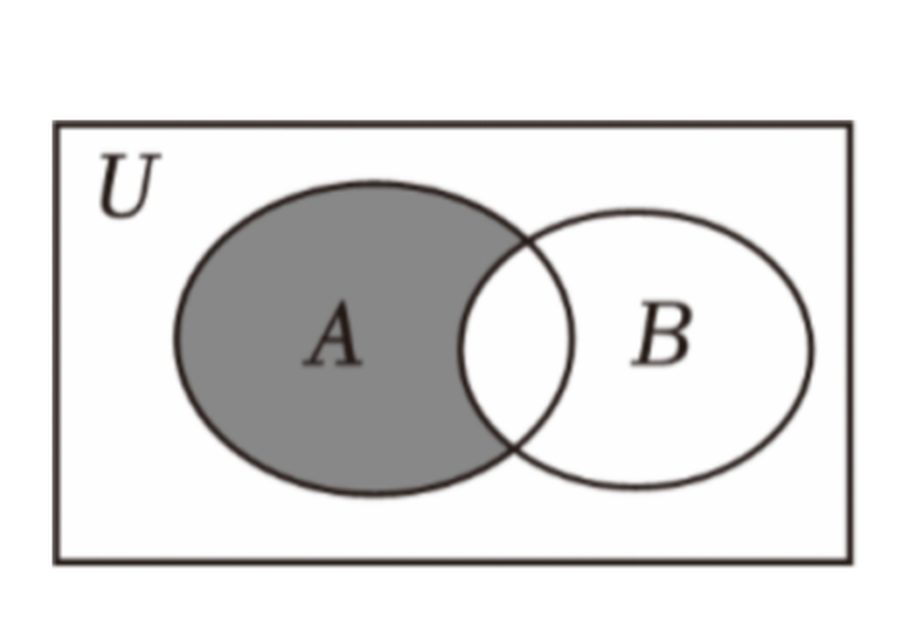
\includegraphics[width=0.34\textwidth]{figures/gao123_q17.png}
\end{center}

\ifanswer
\solbegin
\step{（1）$A\cap B=\{x\mid2\leqslant x\leqslant4\}$，}
\step{则图中阴影部分表示 $\overline{A\cap B}=\{x\mid-2\leqslant x<2\}$.}% 原卷把上划线盖在整个 $A\cap B$ 上，照录
\step{（2）由题意得 $\overline B=\{x\mid-6\leqslant x<2\}$，$C\subseteq B$，}
\step{所以当 $C=\varnothing$ 时，$10-a\geqslant2a+1$，解得 $a\leqslant3$，符合题意；}
\step{当 $C\neq\varnothing$ 时，$\begin{cases}10-a<2a+1\\2a+1\leqslant-6\end{cases}$ 或者 $\begin{cases}10-a<2a+1\\10-a\geqslant2\end{cases}$，}
\step{此时不等式组 $\begin{cases}10-a<2a+1\\2a+1\leqslant-6\end{cases}$ 无解，}
\step{不等式组 $\begin{cases}10-a<2a+1\\10-a\geqslant2\end{cases}$ 的解集为 $3<a\leqslant8$，}
\step{综上，$a$ 的取值范围为 $\{a\mid a\leqslant8\}$.}
\solend
\fi

\item (1) 求不等式：$\lvert x-1\rvert+\lvert x-2\rvert\leqslant5$ 的解集.

(2) 当 $m<1$ 时，解关于 $x$ 的不等式 $\dfrac{m(x-3)}{x+2}>1$.

\ifanswer
\solbegin
\step{(1) 当 $x<1$ 时，$\lvert x-1\rvert+\lvert x-2\rvert\leqslant5\Leftrightarrow-x+1+2-x\leqslant5$，}
\step{解得 $-1\leqslant x<1$；}
\step{当 $1\leqslant x\leqslant2$ 时，$\lvert x-1\rvert+\lvert x-2\rvert\leqslant5\Leftrightarrow x-1+2-x=1\leqslant5$ 恒成立，}
\step{所以 $1\leqslant x\leqslant2$；}
\step{当 $x>2$ 时，$\lvert x-1\rvert+\lvert x-2\rvert\leqslant5\Leftrightarrow x-1+x-2=2x-3\leqslant5$，}
\step{解得 $2<x\leqslant4$.}
\step{综上所述，不等式 $\lvert x-1\rvert+\lvert x-2\rvert\leqslant5$ 的解集为 $[-1,4]$.}
\step{(2) 原不等式变成 $\dfrac{(m-1)x-(3m+2)}{x+2}>0$，$n<1$，所以 $n-1<0$，}% 原卷作 $n<1$、$n-1<0$，与题设 $m<1$ 字母不一致，照录
\step{所以原不等式变成 $\dfrac{x-\dfrac{3m+2}{m-1}}{x+2}<0$，$\dfrac{3m+2}{m-1}-(-2)=\dfrac{5m}{m-1}$，}
\step{所以 $m<0$ 时，$\dfrac{5m}{m-1}>0$，$\dfrac{3m+2}{m-1}>-2$，}
\step{原不等式的解集为 $\left(-2,\dfrac{3m+2}{m-1}\right)$；}
\step{$m=0$ 时，原不等式变成 $1<0$，无解；}
\step{$0<m<1$ 时，$\dfrac{5m}{m-1}<0$，$\dfrac{3m+2}{m-1}<-2$，}
\step{原不等式的解集为 $\left(\dfrac{3m+2}{m-1},-2\right)$.}
\solend
\fi

\item 在园林博览会上，某公司带来了一种智能设备供采购商洽谈采购，并决定大量投放市场，已知该种设备年固定研发成本为 $50$ 万元，每生产一台需另投入 $100$ 元，设该公司一年内生产该设备 $x$ 万台且全部售完，每万台的销售收入 $G(x)$（万元）与年产量 $x$（万台）满足如下关系式：$G(x)=\begin{cases}180-x,0<x\leqslant20\\80+\dfrac{2000}{x}-\dfrac{8000}{x(x-1)},x>20\end{cases}$.

(1) 写出年利润 $W(x)$（万元）关于年产量 $x$（万台）的函数解析式；（利润 $=$ 销售收入 $-$ 成本）

(2) 当年产量为多少万台时，该公司获得的年利润最大，并求出最大利润.

\ifanswer
\solbegin
\step{(1) $W(x)=xG(x)-50-100x=\begin{cases}-50+80x-x^2,0<x\leqslant20\\-20x+1950-\dfrac{8000}{x-1},x>20\end{cases}$；}
\step{(2) 当 $0<x\leqslant20$ 时，$W(x)=-50+80x-x^2=-(x-40)^2+1550$，}
\step{由函数性质得当 $x\leqslant40$ 时严格增，所以当 $x=20$ 时，$W(x)_{max}=1150$，}
\step{当 $x>20$ 时，$W(x)=-20x+1950-\dfrac{8000}{x-1}=-20\left[(x-1)+\dfrac{400}{x-1}\right]+1930$，}
\step{$W(x)=-20\left[(x-1)+\dfrac{400}{x-1}\right]+1930\leqslant-20\times2\sqrt{(x-1)\cdot\dfrac{400}{x-1}}+1930$}
\step{$=1130$，当且仅当 $x-1=\dfrac{400}{x-1}$，即 $x=21$ 时取等号，}
\step{所以 $W(x)_{max}=1130$，}
\step{因为 $1150>1130$，所以当 $x=20$ 时，$W(x)_{max}=1150$，}
\step{即当年产量为 $20$ 万台时，该公司获得的年利润最大，}
\step{最大利润为 $1150$ 万元.}
\solend
\fi

\item 关于 $x$ 的方程 $(x^2-1)^2-2k\lvert x^2-1\rvert+k+1=0(k\in\R)$.

(1) 若方程无实根，求 $k$ 的取值范围；

(2) 若方程有 $4$ 个不等实根，求 $k$ 的取值范围；

(3) 若 $k=a+b$，且满足 $\dfrac1{a+2b}+\dfrac1{a+3}=\dfrac12$，$a>0$，$b>0$，试判断方程根的个数.

\ifanswer
\solbegin
\step{(1) 关于 $x$ 的方程 $(x^2-1)^2-2k\lvert x^2-1\rvert+k+1=0(k\in\R)$，}
\step{令 $t=\lvert x^2-1\rvert$，则 $t\geqslant0$，则原方程转化为 $t^2-2kt+k+1=0(*)$，}
\step{因为关于 $x$ 的方程 $(x^2-1)^2-2k\lvert x^2-1\rvert+k+1=0(k\in\R)$ 无实根，}
\step{所以 $(*)$ 式无实根或实根均小于零，令 $f(t)=t^2-2kt+k+1$，}
\step{①若 $(*)$ 式无实根，则 $\triangle<0$，解得 $\dfrac{1-\sqrt5}{2}<k<\dfrac{1+\sqrt5}{2}$，}
\step{②两根均为负，则 $\begin{cases}\Delta\geqslant0\\t_{\text{对}}=k<0\\f(0)>0\end{cases}$，解得 $-1<k\leqslant\dfrac{1-\sqrt5}{2}$，}
\step{综合①②，得 $k$ 的取值范围是 $\left(-1,\dfrac{1+\sqrt5}{2}\right)$；}
\step{(2) 作函数 $t=\lvert x^2-1\rvert$ 的图象，}
\begin{center}
% 图取原卷截图（第 11 页解析内）、去水印后 2× LANCZOS 放大，仅答案版出
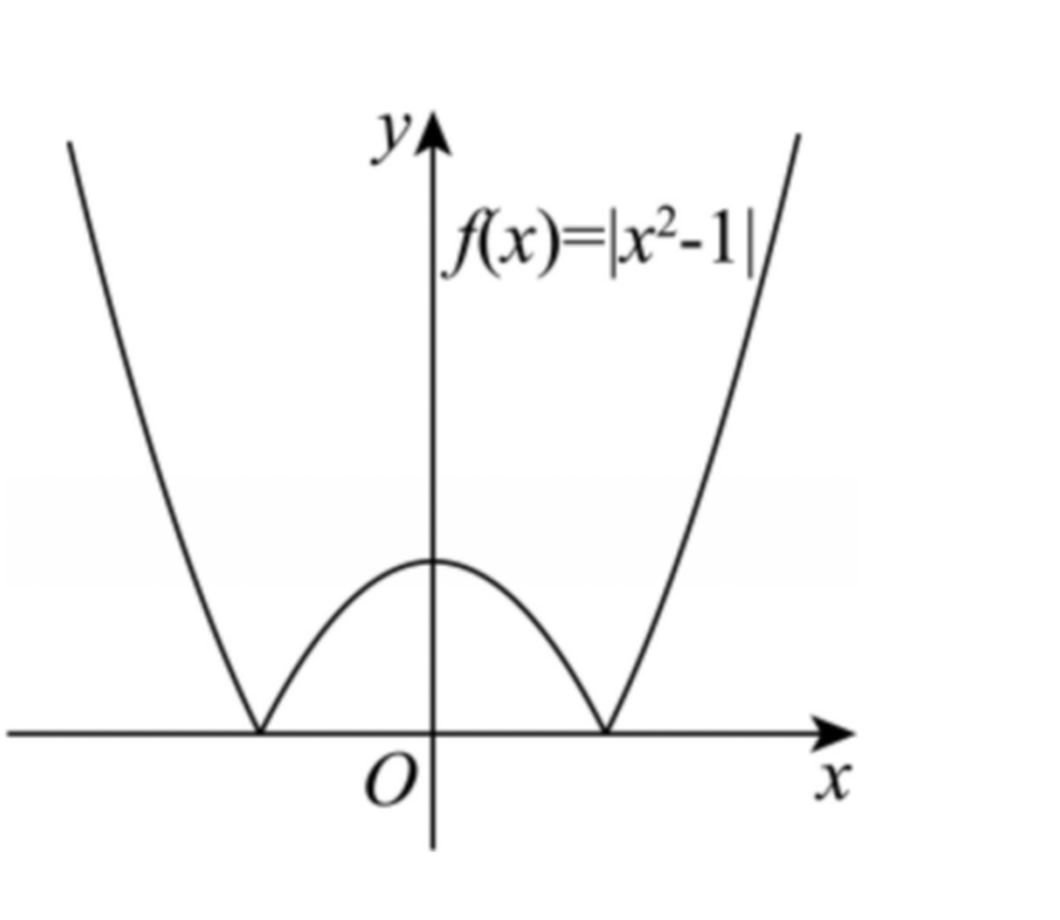
\includegraphics[width=0.40\textwidth]{figures/gao123_q20.png}
\end{center}
\step{$t=0$ 或 $t>1$ 时，每一个 $t$ 值对应 $2$ 个不同的 $x$ 值，}
\step{$t=1$ 时一个 $t$ 值对应 $3$ 个不同的 $x$ 值，}
\step{$0<t<1$ 时一个 $t$ 值对应 $4$ 个不同的 $x$ 值，}
\step{要使原方程有四个不等实根，}
\step{①$(*)$ 式一根为零，另一根大于 $1$，无解；}
\step{②$(*)$ 有两不等根且两根均大于 $1$，则 $\begin{cases}\Delta>0\\t_{\text{对}}=k>1\\f(1)>0\end{cases}$，解得 $\dfrac{1+\sqrt5}{2}<k<2$；}
\step{④$(*)$ 式有 $1$ 实根在 $(0,1)$ 之间，另一根小于零，}% 原卷由 ② 直接跳到 ④，缺 ③，照录
\step{则 $\begin{cases}f(0)<0\\f(1)>0\end{cases}$，所以 $\begin{cases}k+1<0\\2-k>0\end{cases}$，解得 $k<-1$，}
\step{综上所述，$k$ 取值范围为 $(-\infty,-1)\cup\left(\dfrac{1+\sqrt5}{2},2\right)$；}
\step{(3) 因为 $\dfrac1{a+2b}+\dfrac1{a+3}=\dfrac{a+2b+a+3}{(a+2b)(a+3)}=\dfrac{2(a+b)+3}{(a+2b)(a+3)}=\dfrac12$，}
\step{所以 $2(a+b)+3=\dfrac12(a+2b)(a+3)$，}
\step{因为 $a$、$b$ 为正实数，所以 $\dfrac12=\dfrac1{a+2b}+\dfrac1{a+3}\geqslant2\sqrt{\dfrac1{a+2b}\times\dfrac1{a+3}}$，}
\step{得 $\dfrac1{16}\geqslant\dfrac1{a+2b}\times\dfrac1{a+3}$，即 $(a+2b)(a+3)\geqslant16$，}
\step{所以 $2(a+b)+3\geqslant8$，即 $a+b\geqslant\dfrac52$，}
\step{当且仅当 $\dfrac1{a+2b}=\dfrac1{a+3}$ 即 $a=1$,$b=\dfrac32$ 时取等号，}
\step{故 $k\geqslant\dfrac52$，此时有 $\begin{cases}\Delta>0\\t_{\text{对}}=k>1\\f(0)>0,f(1)<0\end{cases}$，}
\step{故 $(*)$ 式有两不等实根且一根在 $(0,1)$ 之间，另一根大于 $1$，}
\step{故原方程有 $6$ 个实根.}
\solend
\fi

\item 设 $n$ 是不小于 $3$ 的正整数，集合 $S_n=\{(a_1,a_2,\cdots,a_n)\mid a_i\in\{0,1\},i=1,2,\cdots,n\}$，对于集合 $S_n$ 中任意两个元素 $A=(a_1,a_2,\cdots,a_n)$，$B=(b_1,b_2,\cdots,b_n)$.

定义 1：$A\cdot B=n-(\lvert a_1-b_1\rvert+\lvert a_2-b_2\rvert+\cdots+\lvert a_n-b_n\rvert)$，

定义 2：若 $A\cdot B=0$，则称互为相反元素，记作 $A=\overline B$ 或 $B=\overline A$.

(1) 若 $n=3$，$A=(0,1,0)$，$B=(1,1,0)$，试写出 $\overline A$、$\overline B$ 以及 $A\cdot B$ 的值；

(2) 若 $A$、$B\in S_n$，$A=(a_1,a_2,\cdots,a_n)$，$B=(b_1,b_2,\cdots,b_n)$，证明：$A\cdot B+\overline A\cdot B=n$；

(3) 设 $k$ 是小于 $n$ 的正奇数，至少含有两个元素的集合 $M\subseteq S_n$，且对于集合 $M$ 中任意两个不相同的元素 $A=(a_1,a_2,\cdots,a_n)$，$B=(b_1,b_2,\cdots,b_n)$，都有 $A\cdot B=n-k$，试求集合 $M$ 中元素个数的所有可能值.

\ifanswer
\solbegin
\step{(1) $\overline A=(1,0,1)$,$\overline B=(0,0,1)$,$\overline A\cdot\overline B=2$；}
\step{(2) 设 $A=(a_1,a_2,\cdots,a_n)$,$B=(b_1,b_2,\cdots,b_n)$,$\overline A=(x_1,x_2,\cdots,x_n)$，}
\step{由 $a_i$、$b_i$、$x_i\in\{0,1\}$，$i=1,2,\cdots,n$，得 $\lvert a_i-x_i\rvert\leqslant1$，$i=1,2,\cdots,n$，}
\step{所以 $\lvert a_1-x_1\rvert+\lvert a_2-x_2\rvert+\cdots+\lvert a_i-x_i\rvert\leqslant n$，}% 原卷末项下标作 $i$，照录
\step{当且仅当 $\lvert a_i-x_i\rvert=1$，$i=1,2,\cdots,n$，}
\step{即 $x_i=1-a_i$，$i=1,2,\cdots,n$ 时取等号.}
\step{由题意得 $A\cdot\overline A=n-(\lvert a_1-x_1\rvert+\lvert a_2-x_2\rvert+\cdots+\lvert a_n-x_n\rvert)=0$，}
\step{即 $\lvert a_1-x_1\rvert+\lvert a_2-x_2\rvert+\cdots+\lvert a_n-x_n\rvert=n$，}
\step{所以 $x_i=1-a_i$，$i=1,2,\cdots,n$，}
\step{$A\cdot B+\overline A\cdot B=2n-\sum\limits_{i=1}^n[\lvert a_i-b_i\rvert+(1-a_i)-b_i]$}
\step{$=2n-\sum\limits_{i=1}^n(\lvert1-b_i\rvert+\lvert0-b_i\rvert)=2n-\sum\limits_{i=1}^n(1-b_i+b_i)=2n-n=n$；}
\step{(3) 假设 $A=(a_1,a_2,\cdots,a_n)$，$B=(b_1,b_2,\cdots,b_n)$，$C=(c_1,c_2,\cdots,c_n)$}
\step{为集合 $M$ 中的三个不相同的元素，}
\step{则 $A\cdot B=n-(\lvert a_1-b_1\rvert+\lvert a_2-b_2\rvert+\cdots+\lvert a_n-b_n\rvert)=n-k$，}
\step{即 $\lvert a_1-b_1\rvert+\lvert a_2-b_2\rvert+\cdots+\lvert a_n-b_n\rvert=k$，}
\step{又由题意得 $\lvert a_i-b_i\rvert=0$ 或 $1$，$i=1,2,\cdots,n$，}
\step{$\lvert a_1-b_1\rvert$、$\lvert a_2-b_2\rvert$、$\cdots$、$\lvert a_n-b_n\rvert$ 恰有 $k$ 个 $1$，$n-k$ 个 $0$，}
\step{设其中 $k$ 个等于 $1$ 的项以此为 $a_{m_1}-b_{m_1}$,$a_{m_2}-b_{m_2}$,$\cdots$,$a_{m_k}-b_{m_k}$，}
\step{$n-k$ 个等于 $0$ 的项为 $a_{m_{k+1}}-b_{m_{k+1}}$,$a_{m_{k+2}}-b_{m_{k+2}}$,$\cdots$,$a_{m_n}-b_{m_n}$，}
\step{由题意得 $A\cdot C=n-(\lvert a_1-c_1\rvert+\lvert a_2-c_2\rvert+\cdots+\lvert a_n-c_n\rvert)=n-k$，}
\step{所以 $\sum\limits_{i=1}^k\lvert a_{m_i}-c_{m_i}\rvert+\sum\limits_{j=k+1}^n\lvert a_{m_j}-c_{m_j}\rvert=k$ ①，}
\step{同理 $\sum\limits_{i=1}^k\lvert b_{m_i}-c_{m_i}\rvert+\sum\limits_{j=k+1}^n\lvert b_{m_j}-c_{m_j}\rvert=k$ ②，}
\step{因为 $\lvert a_{m_{k+1}}-b_{m_{k+1}}\rvert=\lvert a_{m_{k+2}}-b_{m_{k+2}}\rvert=\cdots=\lvert a_{m_n}-b_{m_n}\rvert=0$，}
\step{所以 $\sum\limits_{j=k+1}^n\lvert a_{m_j}-c_{m_j}\rvert=\sum\limits_{j=k+1}^n\lvert b_{m_j}-c_{m_j}\rvert$，}
\step{由①$-$②得 $\sum\limits_{i=1}^k(\lvert a_{m_i}-c_{m_i}\rvert-\lvert b_{m_i}-c_{m_i}\rvert)=0$，}
\step{又 $\sum\limits_{i=1}^k(\lvert a_{m_i}-c_{m_i}\rvert-\lvert b_{m_i}-c_{m_i}\rvert)=\sum\limits_{i=1}^k(\lvert1-c_{m_i}\rvert-\lvert0-c_{m_i}\rvert)=k-2\sum\limits_{i=1}^k c_{m_i}$}
\step{为奇数，与 $\sum\limits_{i=1}^k(\lvert a_{m_i}-c_{m_i}\rvert-\lvert b_{m_i}-c_{m_i}\rvert)=0$ 矛盾，所以假设不成立，}
\step{即集合 $M$ 中至多有两个元素，}
\step{当 $M=\{(1,1,\cdots,1,0,0,\cdots,0),(0,0,\cdots,0)\}$ 时符合题意，}
\step{所以集合 $M$ 中元素的个数只可能是 $2$.}
\solend
\fi

\end{enumerate}

\end{document}
"
% 紧凑版：xelatex "\def\iscompact{1}% 高一123_行知中学_10月月考.tex
%   —— 高一上数学“2026-2027 年行知中学高一上 10 月月考”（试卷版/答案版）
% 试卷版：xelatex 高一123_行知中学_10月月考.tex
% 答案版：xelatex "\def\isanswer{1}\input{高一123_行知中学_10月月考.tex}"
% 紧凑版：xelatex "\def\iscompact{1}\input{高一123_行知中学_10月月考.tex}"
%
% 原始材料：微信公众号“魔都数学加油站”文章，作者破晓，2026-11-09 17:52 发布；
% 连载“27学年高一123”，原文标题“27学年高一123——2026-2027年上海市行知中学高一上10月月考”；
% 原文链接：https://mp.weixin.qq.com/s/GV4SWBLUJrBhMQwo22FVzg。
% 正文为 14 张 PNG 页（第 7、9、11、13、14 页 2560×3620，其余 4762×6735），
% 题目下印有【答案】或【解析】，为讲评版。
% 题目、解析均据原图转录；卷面红色水印及公众号页脚未录入。
% 全卷 3 张插图：第 5 题的坐标示意图、第 17 题的文氏图（均属题干，三版都出）、
% 第 20 题 (2) 的 $t=\lvert x^2-1\rvert$ 图象（属解析，仅答案版出）；
% 都取原卷截图去水印、2× LANCZOS 放大，见 figures/gao123_q5.png、
% figures/gao123_q17.png、figures/gao123_q20.png。
%
% 卷首标题：原卷印作“2026-2027 年行知中学高一上 10 月月考”（公众号标题中的“上海市”
% 卷面标题行没有，本稿照卷面），年份区间按全稿惯例排 en dash；原卷未印副标题，本稿按题目内容
% 标为“集合与常用逻辑用语、不等式”（与 110／111／113／116／118／120 同）。
%
% 与原卷的排版差异：
%   ① 原文从第 3 题起，填空题编号为 3—12、选择题为 13—16、解答题为 17—21，本稿保留原题号；
%   ② 原卷每题下直接印【解析】／【答案】，本稿按全稿惯例置于答案版；第 3 题只印【答案】、
%      另提 \ans{}；选择题答案在解析末句“故选 …”，括号内留空；
%   ③ 原卷未印副标题，本稿按“知识模块”口径补出；
%   ④ 原卷填空横线按全稿惯例排为 \blankline[4.4em]；选择题括号排 \mbox{（\quad）}、
%      选项段前按惯例加 \keepwithprev；解答题不留作答区（原卷为讲评版，与 109—122 同）；
%   ⑤ 原卷数集排斜体 $R$／$Z$（第 9 题作粗体 $\mathbf{R}$），按全稿惯例改 \R／\Z；
%      绝对值按全稿惯例排 \lvert…\rvert，集合描述竖线排 \mid；单位 km、h 原卷排斜体，
%      本稿按正体照排；补集照原卷上划线排 \overline{B}、\overline{A}。
%
% 判别式与子集符号：第 16 题解析的 $\triangle=b^2-4c<0$、第 20 题 (1) ① 的 $\triangle<0$
%   均作等边、扁的 \triangle；第 20 题 ② 两处 cases 与 (3) 的 $\Delta\geqslant0$／$\Delta>0$
%   作等腰、高的 \Delta，逐处照录、不统一；第 15 题选项与第 17 题 (2) 的 $\subseteq$
%   印有下划线，照录 \subseteq。
%
% 原卷存疑照录：
%   第 4 题解析“若 $-\lvert a\rvert=0$，则 $a=0$，则 $A=\{0,-1,0\}$”以元素重复说明互异性；
%   第 5 题解析“当 $a^2+b^2=400^2+b^2<500^2$”等式左边 $a^2$ 与 $400^2$ 并用；
%   第 9 题解析“解得 $a>1$ 得 $a<\dfrac13$”（按平方不等式应为 $a>1$ 或 $a<\dfrac13$）；
%   第 12 题解析“所以 $-\dfrac1{2^a}\cdot\dfrac1{2^b}\geqslant-\dfrac14$”带负号起论；
%   第 17 题 (1) 解析把阴影部分（实为 $A\cap\overline B$）印作 $\overline{A\cap B}$；
%   第 18 题 (2) 解析作“$n<1$，所以 $n-1<0$”，与题设 $m<1$ 字母不一致；
%   第 20 题 (2) 的情形编号由 ①、② 直接跳到 ④（缺 ③）；
%   第 21 题 (2) 解析“$\lvert a_1-x_1\rvert+\cdots+\lvert a_i-x_i\rvert\leqslant n$”
%   末项下标作 $i$（按上下文应为 $n$）。以上均照录加注。
%
% 行数核对：逐题数 \step 条数，合计 176 条（Q3：0；Q4：6；Q5：5；Q6：5；Q7：4；
% Q8：6；Q9：5；Q10：5；Q11：10；Q12：6；Q13：9；Q14：1；Q15：5；Q16：21；
% Q17：8；Q18：14；Q19：10；Q20：26；Q21：30），与原卷印刷行逐题相等
% （cases 块作一个印刷行计）。第 3 题只印【答案】，提 \ans{}，不计入 \step 账。
%
\documentclass[a4paper,11pt]{article}
\usepackage{common}

\begin{document}

\examtitlest[3]{2026--2027 年行知中学高一上 10 月月考}{集合与常用逻辑用语、不等式}

\bigsec{一、填空题}

\begin{enumerate}
\setcounter{enumi}{2}

\item 写出命题“存在实数 $x$、$y$、$z$，使 $x<y$ 或 $y<z$.”的否定\blankline[4.4em].

\ifanswer
\ans{任意实数 $x$、$y$、$z$，使得 $x\geqslant y$ 且 $y\geqslant z$}
\fi

\item 若集合 $\{0,-1,2a\}=\{a-1,-\lvert a\rvert,a+1\}$，实数 $a$ 的值为\blankline[4.4em].

\ifanswer
\solbegin
\step{令 $A=\{0,-1,2a\}$,$B=\{a-1,-\lvert a\rvert,a+1\}$，}
\step{因为 $\{0,-1,2a\}=\{a-1,-\lvert a\rvert,a+1\}$，}
\step{若 $a-1=0$，则 $a=1$，则 $A=\{0,-1,2\}$,$B=\{0,-1,2\}$，满足要求；}
\step{若 $-\lvert a\rvert=0$，则 $a=0$，则 $A=\{0,-1,0\}$，不满足集合元素的互异性；}% 原卷以 $A=\{0,-1,0\}$ 说明互异性，照录
\step{若 $a+1=0$，则 $a=-1$，则 $A=\{0,-1,-2\}$,$B=\{0,-1,-2\}$，满足要求；}
\step{故实数 $a$ 的值为 $\pm1$.}
\solend
\fi

\needvspace{7cm}
\item 如图，据气象部门预报，在距离某码头南偏东 $45^\circ$ 方向 $400\sqrt2$ km 处的热带
风暴中心正在以 $20$km/h 的速度向正北方向移动，距风暴中心 $500$km 以内
的地区都将受到影响. 以上预报估计，该码头将受到热带风暴的影响时长大
约为\blankline[4.4em]$h$.

\begin{center}
% 图取原卷截图（第 1 页题干右侧）、去水印后 2× LANCZOS 放大，本稿移至题干之后
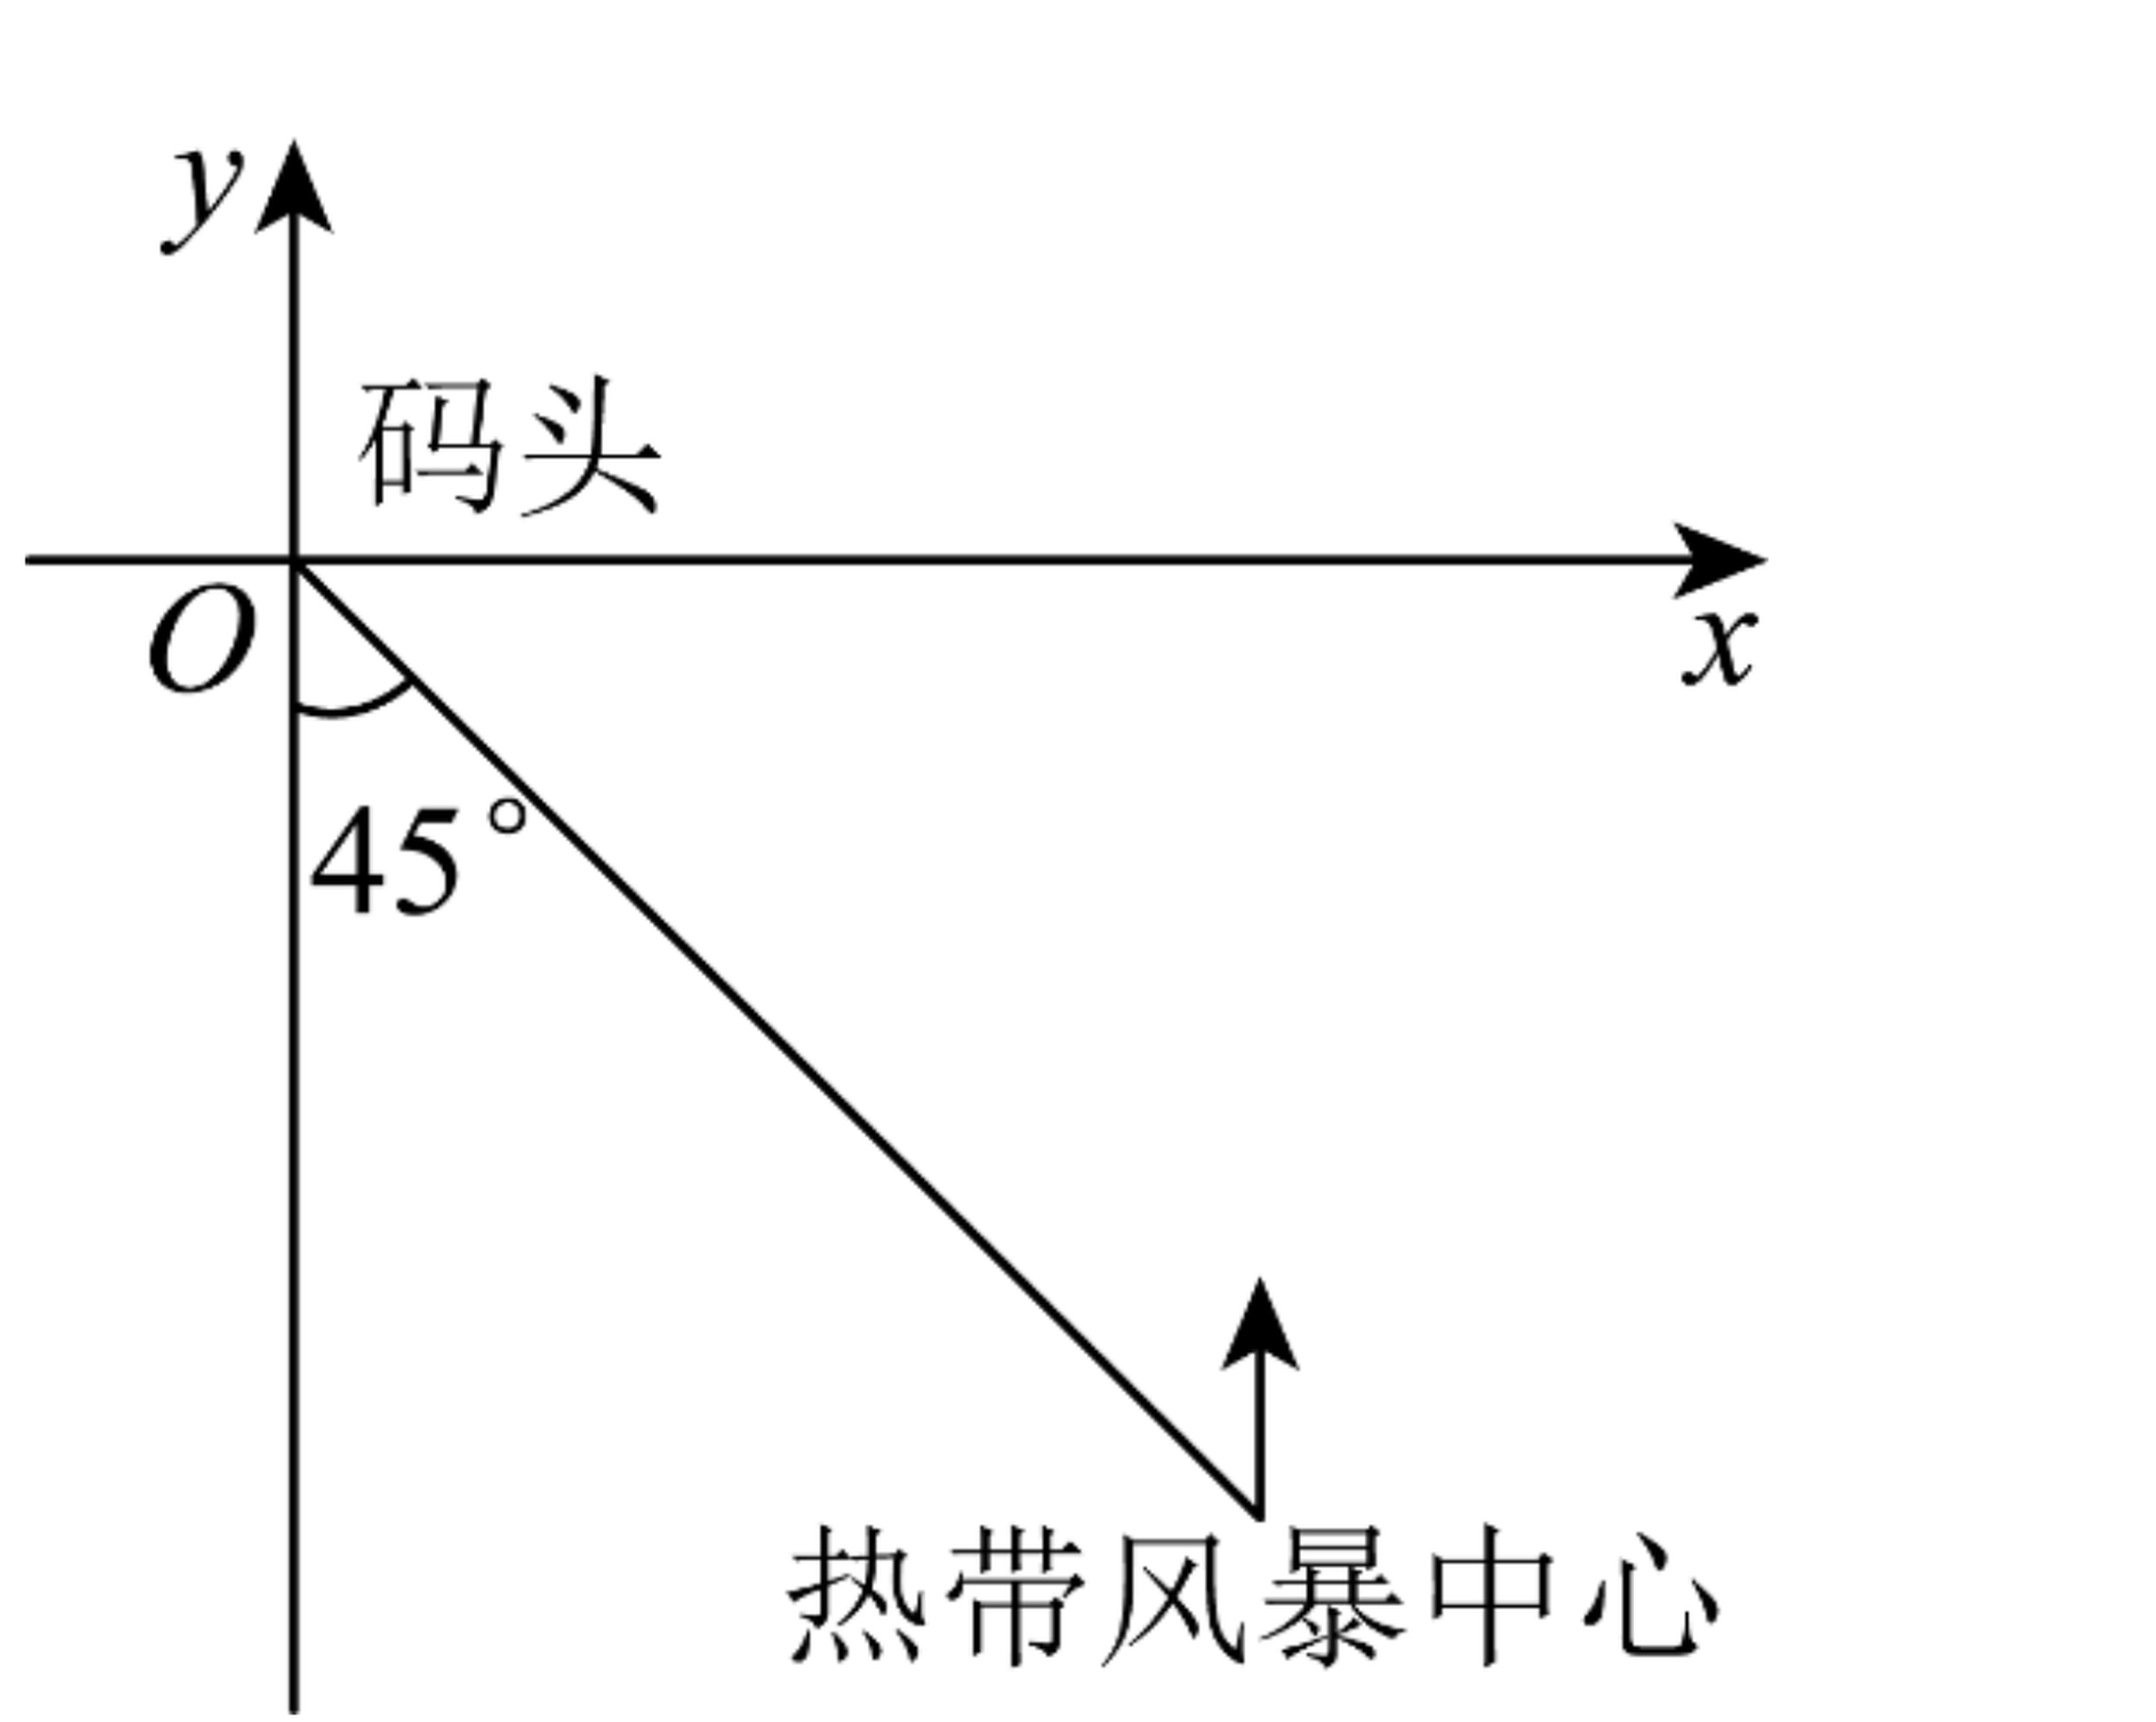
\includegraphics[width=0.36\textwidth]{figures/gao123_q5.png}
\end{center}

\ifanswer
\solbegin
\step{设风暴中心的坐标为 $(a,b)$，}
\step{由题意得 $a=400\sqrt2\times\cos45^\circ=400$，当 $a^2+b^2=400^2+b^2<500^2$，}% 原卷 $a^2$ 与 $400^2$ 并用，照录
\step{即 $-300<b<300$ 时，码头将受到风暴影响，}
\step{$\dfrac{300-(-300)}{20}=30h$，则码头受到风暴影响的时长为 30 小时，}
\step{所以由预报估计，该码头将受到热带风暴的影响时长大约为 30 小时.}
\solend
\fi

\item 已知 $a$、$b$、$c$ 为常数，若不等式 $\dfrac{ax-b}{x-c}\geqslant0$ 的解集为 $[-1,1)$，则不等式 $ax+b<0$ 的解集为\blankline[4.4em].

\ifanswer
\solbegin
\step{不等式 $\dfrac{ax-b}{x-c}\geqslant0$ 可化为 $(ax-b)(x-c)\geqslant0$ 且 $x-c\neq0$，}
\step{即 $a\left(x-\dfrac ba\right)(x-c)\geqslant0$ 且 $x\neq c$，}
\step{因为不等式 $\dfrac{ax-b}{x-c}\geqslant0$ 的解集为 $[-1,1)$，所以 $a<0$，且 $\dfrac ba=-1$,$c=1$，}
\step{即 $b=-a$，所以不等式 $ax+b<0$ 可化为 $ax-a<0$，又因为 $a<0$，所以 $x-1>0$，}
\step{解得 $x>1$，所以不等式 $ax+b<0$ 的解集为 $(1,+\infty)$.}
\solend
\fi

\item 已知实数 $a$、$b$ 满足 $ab=32$，且 $\log_2a=\log_b16$，则 $a+b$ 的值为\blankline[4.4em].

\ifanswer
\solbegin
\step{由 $\log_2a=\log_b16$，得 $\log_2a=\dfrac{\log_216}{\log_2b}$，则 $\log_2a\cdot\log_2b=4$，}
\step{由 $ab=32$，得 $\log_2a+\log_2b=\log_2ab=5$，}
\step{得 $\log_2a=1$,$\log_2b=4$ 或 $\log_2a=4$,$\log_2b=1$，}
\step{因此 $a=2$,$b=16$ 或 $a=16$,$b=2$，所以 $a+b=18$.}
\solend
\fi

\item 已知实数 $a$、$b$ 满足 $-3<a+2b<2$，$-1<2a-b<4$，则 $a+b$ 的取值范围为\blankline[4.4em].

\ifanswer
\solbegin
\step{设 $a+b=m(a+2b)+n(2a-b)=(m+2n)a+(2m-n)b$，}
\step{所以 $\begin{cases}m+2n=1\\2m-n=1\end{cases}$，解得 $n=\dfrac15$,$m=\dfrac35$，所以 $a+b=\dfrac35(a+2b)+\dfrac15(2a-b)$，}
\step{因为 $-3<(a+2b)<2$，$-1<2a-b<4$，}
\step{所以 $-\dfrac95<\dfrac35(a+2b)<\dfrac65$，$-\dfrac15<\dfrac15(2a-b)<\dfrac45$，}
\step{相加得 $-2<\dfrac35(a+2b)+\dfrac15(2a-b)<2$，即 $-2<a+b<2$，}
\step{故 $a+b$ 的取值范围为 $(-2,2)$.}
\solend
\fi

\item 存在 $x\in\R$ 使不等式 $\lvert2x-a\rvert<\lvert2a-1\rvert-2\lvert x\rvert$ 成立，则实数 $a$ 的取值范围是\blankline[4.4em].

\ifanswer
\solbegin
\step{存在 $x\in\R$，不等式 $\lvert2x-a\rvert<\lvert2a-1\rvert-2\lvert x\rvert$ 成立，}
\step{变形即 $\lvert2x-a\rvert+2\lvert x\rvert<\lvert2a-1\rvert$ 成立，}
\step{由于 $\lvert2x-a\rvert+\lvert2x\rvert\geqslant\lvert(2x-a)-2x\rvert=\lvert a\rvert$，当且仅当 $2x(2x-a)\leqslant0$ 时取等号，}
\step{因此有 $\lvert a\rvert<\lvert2a-1\rvert$，两边平方 $a^2<(2a-1)^2$，解得 $a>1$ 得 $a<\dfrac13$，}% 原卷“解得 a>1 得 a<1/3”，照录
\step{即实数 $a$ 的取值范围是 $\left(-\infty,\dfrac13\right)\cup(1,+\infty)$.}
\solend
\fi

\item 已知集合 $A=\{(x,y)\mid x^2+mx-y+2=0\}$，$B=\{(x,y)\mid x-y+1=0,0\leqslant x\leqslant3\}$，若集合 $A\cap B$ 的子集个数为 $2$，则实数 $m$ 的取值范围为\blankline[4.4em].

\ifanswer
\solbegin
\step{因为集合 $A\cap B$ 的子集个数为 $2$，所以 $A\cap B$ 的元素有一个，}
\step{即 $\begin{cases}x^2+mx-y+2=0\\x-y+1=0\end{cases}$ 在 $x\in[0,3]$ 上只有一个解，}
\step{即 $x^2+(m-1)x+1=0$ 在 $[0,3]$ 上只有一个解，}
\step{即 $1-m=x+\dfrac1x$ 在 $[0,3]$ 上只有一个解，}
\step{结合对勾函数的性质得 $1-m=2$ 或 $1-m>\dfrac{10}{3}$，解得 $m=-1$ 或 $m<-\dfrac73$.}
\solend
\fi

\item $[x]$ 表示不超过 $x$ 的最大整数，则集合 $A=\left\{y\,\middle\vert\,y=\left[\dfrac{x^2}{100}\right],x=1,2,3,\cdots,100\right\}$ 中的元素个数为\blankline[4.4em].

\ifanswer
\solbegin
\step{记 $a_k=\left[\dfrac{k^2}{100}\right](k=1,2,\cdots,100)$，$a_k$ 随 $k$ 增大而单调不减.}
\step{当 $k\geqslant50$ 时，$\dfrac{(k+1)^2}{100}-\dfrac{k^2}{100}=\dfrac{2k+1}{100}\geqslant\dfrac{101}{100}>1$，所以 $a_{k+1}\geqslant a_k+1$，}
\step{即 $a_{50}$、$a_{51}$、$\cdots$、$a_{100}$ 两两互异.}
\step{又 $a_{50}=\left[\dfrac{2500}{100}\right]=25$、$a_{100}=100$，这一段共 $100-50+1=51$ 个互异的值，}
\step{且都大于等于 $25$.}
\step{当 $k\leqslant49$ 时，$\dfrac{(k+1)^2}{100}-\dfrac{k^2}{100}=\dfrac{2k+1}{100}\leqslant\dfrac{99}{100}<1$，即 $a_k$ 每次至多增加 $1$；}
\step{又 $a_1=0$、$a_{49}=\left[\dfrac{2401}{100}\right]=24$，}
\step{故 $a_1$、$a_2$、$\cdots$、$a_{49}$ 依次取遍 $0$，$1$，$2$，$\cdots$，$24$，共 $25$ 个值.}
\step{两段取值范围互不重叠（前段不超过 $24$、后段不小于 $25$），}
\step{所以集合 $A$ 中共有 $25+51=76$ 个元素.}
\solend
\fi

\item 若实数 $a$、$b$、$c$ 满足 $\dfrac1{2^a}+\dfrac1{2^b}=1$，$\dfrac1{2^{a+b}}+\dfrac1{2^{b+c}}+\dfrac1{2^{a+c}}=1$，则 $c$ 的最大值是\blankline[4.4em].

\ifanswer
\solbegin
\step{因为 $\dfrac1{2^a}+\dfrac1{2^b}=1$，}
\step{由基本不等式得 $1=\dfrac1{2^a}+\dfrac1{2^b}\geqslant2\sqrt{\dfrac1{2^a}\cdot\dfrac1{2^b}}$（当且仅当 $a=b=1$ 时取等号），}
\step{所以 $\dfrac1{2^a}\cdot\dfrac1{2^b}\leqslant\dfrac14$，所以 $-\dfrac1{2^a}\cdot\dfrac1{2^b}\geqslant-\dfrac14$，}% 原卷带负号起论，照录
\step{因为 $\dfrac1{2^{a+b}}+\dfrac1{2^{b+c}}+\dfrac1{2^{a+c}}=1$，$\dfrac1{2^{b+c}}+\dfrac1{2^{a+c}}=\dfrac1{2^c}\left(\dfrac1{2^a}+\dfrac1{2^b}\right)=\dfrac1{2^c}$，}
\step{所以 $\dfrac1{2^c}=1-\dfrac1{2^{a+b}}\geqslant\dfrac34$，所以 $2^c\leqslant\dfrac43$，所以 $c\leqslant\log_2\dfrac43=2-\log_23$，}
\step{故 $c$ 的最大值是 $2-\log_23$.}
\solend
\fi

\end{enumerate}

\bigsec{二、选择题}

\begin{enumerate}
\setcounter{enumi}{12}

\item 下列运用等式或不等式的性质变形中，正确的是\mbox{（\quad）}

\keepwithprev
A. 如果 $a=b$，那么 $\dfrac ac=\dfrac bc$\qquad\qquad B. 如果 $\dfrac1a<\dfrac1b<0$，那么 $a-\dfrac1a>b-\dfrac1b$

C. 如果 $a>b$，那么 $\dfrac1a<\dfrac1b$\qquad\qquad D. 如果 $a>b>0$，$m\in\R$，那么 $\dfrac ba<\dfrac{b+m}{a+m}$

\ifanswer
\solbegin
\step{对于 $A$，若 $c=0$，$A$ 错误；}
\step{对于 $B$，若 $\dfrac1a<\dfrac1b<0$，则 $0>a>b$，$-\dfrac1a>-\dfrac1b>0$，}
\step{所以 $a-\dfrac1a>b-\dfrac1b$，$B$ 正确；}
\step{对于 $C$，$a>0$，$b<0$ 时，$C$ 错误；}
\step{对于 $D$，$\dfrac{b+m}{a+m}-\dfrac ba=\dfrac{ab+am}{a(a+m)}-\dfrac{ab+bm}{a(a+m)}=\dfrac{(a-b)m}{a(a+m)}$，}
\step{因为 $a>b>0$，所以 $a-b>0$，但 $m$、$a+m$ 的符号不确定，}
\step{当 $m=0$ 时，$\dfrac ba=\dfrac{b+m}{a+m}$，}
\step{当 $m(a+m)>0$ 时，$\dfrac ba<\dfrac{b+m}{a+m}$，当 $m(a+m)<0$ 时，$\dfrac ba>\dfrac{b+m}{a+m}$，$D$ 错误.}
\step{故选 $B$.}
\solend
\fi

\item “$a>b$”的一个必要非充分条件是\mbox{（\quad）}

\keepwithprev
A. $ac^2>bc^2$\qquad\quad B. $2^a>2^b$\qquad\quad C. $\left(\dfrac12\right)^{a-b}\leqslant1$\qquad\quad D. $a^3>b^3$

\ifanswer
\solbegin
\step{即“$a>b$”能推出选项，但选项不能推出“$a>b$”，故选 $C$.}
\solend
\fi

\item 若 $A=\left\{x\,\middle\vert\,x=\dfrac k6+1,k\in\Z\right\}$，$B=\left\{x\,\middle\vert\,x=\dfrac k3+\dfrac12,k\in\Z\right\}$，$C=\left\{x\,\middle\vert\,x=\dfrac{2k}{3}+\dfrac12,k\in\Z\right\}$，则这三个集合间的关系是\mbox{（\quad）}

\keepwithprev
A. $A\subseteq B\subseteq C$\qquad\quad B. $A\subseteq C\subseteq B$\qquad\quad C. $C\subseteq B\subseteq A$\qquad\quad D. $C\subseteq A\subseteq B$

\ifanswer
\solbegin
\step{若 $x\in C$，则存在 $k_0\in\Z$，使 $x=\dfrac{2k_0}{3}+\dfrac12$，}
\step{又 $2k_0\in\Z$，所以 $x\in B$，故 $C\subseteq B$，}
\step{若 $x\in B$，则存在 $k_1\in\Z$，使 $x=\dfrac{k_1}{3}+\dfrac12=\dfrac{2k_1-3}{6}+1$，}
\step{又 $2k_1-3\in\Z$，所以 $x\in A$，故 $B\subseteq A$，}
\step{又 $\dfrac43\in A$，$\dfrac43\notin B$，$\dfrac56\in B$，$\dfrac56\notin C$，所以 $C\subseteq B\subseteq A$，故选 $C$.}
\solend
\fi

\item 集合 $S=\{x\mid(x+a)(x^2+bx+c)=0\}$，$T=\{x\mid(ax+1)(cx^2+bx+1)=0\}$，其中 $a$、$b$、$c$ 为实数，若 $\lvert S\rvert$、$\lvert T\rvert$ 分别表示 $S$、$T$ 的元素个数，则下列结论中一定成立的是\mbox{（\quad）}

\keepwithprev
A. 若 $\lvert T\rvert=0$，则 $\lvert S\rvert=1$\qquad\qquad B. 若 $\lvert S\rvert=1$，则 $\lvert T\rvert=1$

C. 若 $\lvert S\rvert=2$，则 $\lvert T\rvert=2$\qquad\qquad D. 若 $\lvert T\rvert=3$，则 $\lvert S\rvert=2$

\ifanswer
\solbegin
\step{令 $f(x)=(x+a)(x^2+bx+c)$,$g(x)=(ax+1)(cx^2+bx+1)$，}
\step{对于选项 A，当 $\lvert T\rvert=0$ 时，方程 $g(x)=(ax+1)(cx^2+bx+1)=0$ 无实根，}
\step{当 $a=b=c=0$ 时，$f(x)=x^3$，由 $f(x)=0$ 得 $x=0$，此时 $\lvert S\rvert=1$；}
\step{当 $a=0$,$b^2-4c<0$ 时，$f(x)=x(x^2+bx+c)$，由 $f(x)=0$ 得 $x=0$，}
\step{此时 $\lvert S\rvert=1$，所以选项 A 正确；}
\step{对于选项 B，若 $\lvert S\rvert=1$，则 $f(x)=(x+a)(x^2+bx+c)=0$ 有且只有一根，}
\step{又 $x=-a$ 一定是 $f(x)=0$ 的根，所以 $\triangle=b^2-4c<0$，}
\step{又 $\triangle=b^2-4c<0$ 且 $a=0$ 时，$g(x)=(ax+1)(cx^2+bx+1)=0$ 无解，}
\step{此时 $\lvert T\rvert=0$，所以选项 B 错误，}
\step{对于选项 C，若 $\lvert S\rvert=2$ 时，则 $f(x)=(x+a)(x^2+bx+c)=0$ 有且只有 $2$ 根，}
\step{又 $x=-a$ 一定是 $f(x)=0$ 的根，}
\step{所以 $\triangle=b^2-4c=0$ 且 $a^2+ab+c\neq0$ 或 $\triangle=b^2-4c>0$ 且 $a^2+ab+c=0$，}
\step{当 $a=0$ 时，存在 $b$,$c$，使 $\triangle=b^2-4c=0$ 且 $a^2+ab+c\neq0$，}
\step{此时 $g(x)=(ax+1)(cx^2+bx+1)=0$ 只有一根，所以选项 C 错误，}
\step{对于选项 D，当 $\lvert T\rvert=3$ 时，方程 $g(x)=(ax+1)(cx^2+bx+1)=0$ 有三个根，}
\step{所以 $a\neq0$,$c\neq0$,$b^2-4c>0$，}
\step{设 $x_0$ 为 $g(x)=0$ 的一个根，即 $(ax_0+1)(cx_0^2+bx_0+1)=0$，}
\step{则 $x_0\neq0$，且 $f\left(\dfrac1{x_0}\right)=\left(\dfrac1{x_0}+a\right)\left(\dfrac1{x_0^2}+\dfrac1{x_0}b+c\right)=\dfrac1{x_0^3}g(x_0)=0$，}
\step{所以 $\dfrac1{x_0}$ 为方程 $f(x)=0$ 的根，故 $f(x)=0$ 有三个根，即 $\lvert T\rvert=3$ 时，}
\step{必有 $\lvert S\rvert=3$，所以选项 D 错误，}
\step{故选 $A$.}
\solend
\fi

\end{enumerate}

% 第 17 题是解答题第一题且带文氏图，守卫放在 \bigsec 之前，连节标题一起量页高
\needvspace{7cm}
\bigsec{三、解答题}

\begin{enumerate}
\setcounter{enumi}{16}

\item 设全集 $U=\R$，集合 $A=\{x\mid-2\leqslant x\leqslant4\}$，$B=\{x\mid x<-6$ 或 $x\geqslant2\}$.

（1）求图中阴影部分表示的集合；

（2）已知集合 $C=\{x\mid10-a<x<2a+1\}$，若 $\overline B\cap C=\varnothing$，求 $a$ 的取值范围.

\begin{center}
% 图取原卷截图（第 7 页题干右侧）、去水印后 2× LANCZOS 放大，本稿移至题干之后
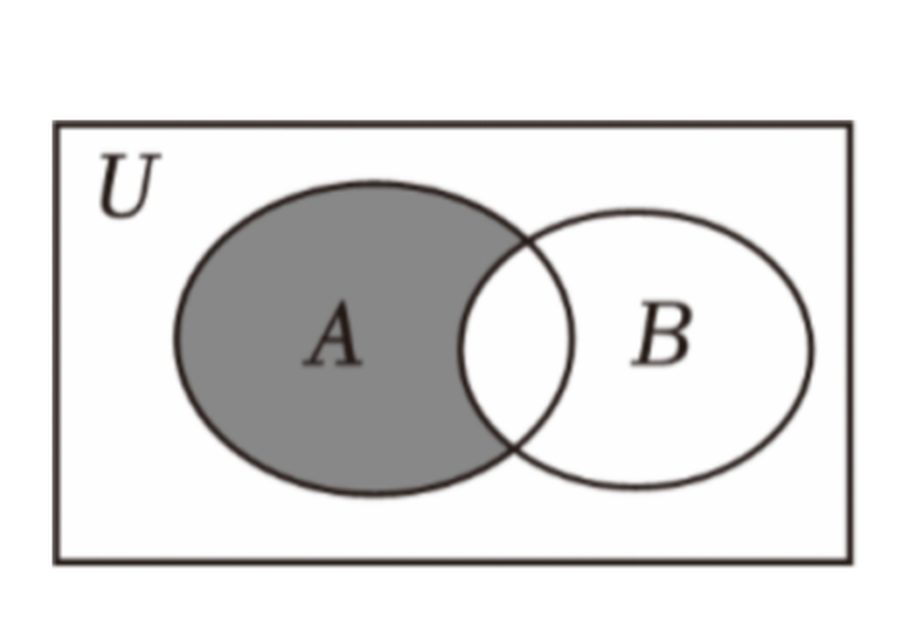
\includegraphics[width=0.34\textwidth]{figures/gao123_q17.png}
\end{center}

\ifanswer
\solbegin
\step{（1）$A\cap B=\{x\mid2\leqslant x\leqslant4\}$，}
\step{则图中阴影部分表示 $\overline{A\cap B}=\{x\mid-2\leqslant x<2\}$.}% 原卷把上划线盖在整个 $A\cap B$ 上，照录
\step{（2）由题意得 $\overline B=\{x\mid-6\leqslant x<2\}$，$C\subseteq B$，}
\step{所以当 $C=\varnothing$ 时，$10-a\geqslant2a+1$，解得 $a\leqslant3$，符合题意；}
\step{当 $C\neq\varnothing$ 时，$\begin{cases}10-a<2a+1\\2a+1\leqslant-6\end{cases}$ 或者 $\begin{cases}10-a<2a+1\\10-a\geqslant2\end{cases}$，}
\step{此时不等式组 $\begin{cases}10-a<2a+1\\2a+1\leqslant-6\end{cases}$ 无解，}
\step{不等式组 $\begin{cases}10-a<2a+1\\10-a\geqslant2\end{cases}$ 的解集为 $3<a\leqslant8$，}
\step{综上，$a$ 的取值范围为 $\{a\mid a\leqslant8\}$.}
\solend
\fi

\item (1) 求不等式：$\lvert x-1\rvert+\lvert x-2\rvert\leqslant5$ 的解集.

(2) 当 $m<1$ 时，解关于 $x$ 的不等式 $\dfrac{m(x-3)}{x+2}>1$.

\ifanswer
\solbegin
\step{(1) 当 $x<1$ 时，$\lvert x-1\rvert+\lvert x-2\rvert\leqslant5\Leftrightarrow-x+1+2-x\leqslant5$，}
\step{解得 $-1\leqslant x<1$；}
\step{当 $1\leqslant x\leqslant2$ 时，$\lvert x-1\rvert+\lvert x-2\rvert\leqslant5\Leftrightarrow x-1+2-x=1\leqslant5$ 恒成立，}
\step{所以 $1\leqslant x\leqslant2$；}
\step{当 $x>2$ 时，$\lvert x-1\rvert+\lvert x-2\rvert\leqslant5\Leftrightarrow x-1+x-2=2x-3\leqslant5$，}
\step{解得 $2<x\leqslant4$.}
\step{综上所述，不等式 $\lvert x-1\rvert+\lvert x-2\rvert\leqslant5$ 的解集为 $[-1,4]$.}
\step{(2) 原不等式变成 $\dfrac{(m-1)x-(3m+2)}{x+2}>0$，$n<1$，所以 $n-1<0$，}% 原卷作 $n<1$、$n-1<0$，与题设 $m<1$ 字母不一致，照录
\step{所以原不等式变成 $\dfrac{x-\dfrac{3m+2}{m-1}}{x+2}<0$，$\dfrac{3m+2}{m-1}-(-2)=\dfrac{5m}{m-1}$，}
\step{所以 $m<0$ 时，$\dfrac{5m}{m-1}>0$，$\dfrac{3m+2}{m-1}>-2$，}
\step{原不等式的解集为 $\left(-2,\dfrac{3m+2}{m-1}\right)$；}
\step{$m=0$ 时，原不等式变成 $1<0$，无解；}
\step{$0<m<1$ 时，$\dfrac{5m}{m-1}<0$，$\dfrac{3m+2}{m-1}<-2$，}
\step{原不等式的解集为 $\left(\dfrac{3m+2}{m-1},-2\right)$.}
\solend
\fi

\item 在园林博览会上，某公司带来了一种智能设备供采购商洽谈采购，并决定大量投放市场，已知该种设备年固定研发成本为 $50$ 万元，每生产一台需另投入 $100$ 元，设该公司一年内生产该设备 $x$ 万台且全部售完，每万台的销售收入 $G(x)$（万元）与年产量 $x$（万台）满足如下关系式：$G(x)=\begin{cases}180-x,0<x\leqslant20\\80+\dfrac{2000}{x}-\dfrac{8000}{x(x-1)},x>20\end{cases}$.

(1) 写出年利润 $W(x)$（万元）关于年产量 $x$（万台）的函数解析式；（利润 $=$ 销售收入 $-$ 成本）

(2) 当年产量为多少万台时，该公司获得的年利润最大，并求出最大利润.

\ifanswer
\solbegin
\step{(1) $W(x)=xG(x)-50-100x=\begin{cases}-50+80x-x^2,0<x\leqslant20\\-20x+1950-\dfrac{8000}{x-1},x>20\end{cases}$；}
\step{(2) 当 $0<x\leqslant20$ 时，$W(x)=-50+80x-x^2=-(x-40)^2+1550$，}
\step{由函数性质得当 $x\leqslant40$ 时严格增，所以当 $x=20$ 时，$W(x)_{max}=1150$，}
\step{当 $x>20$ 时，$W(x)=-20x+1950-\dfrac{8000}{x-1}=-20\left[(x-1)+\dfrac{400}{x-1}\right]+1930$，}
\step{$W(x)=-20\left[(x-1)+\dfrac{400}{x-1}\right]+1930\leqslant-20\times2\sqrt{(x-1)\cdot\dfrac{400}{x-1}}+1930$}
\step{$=1130$，当且仅当 $x-1=\dfrac{400}{x-1}$，即 $x=21$ 时取等号，}
\step{所以 $W(x)_{max}=1130$，}
\step{因为 $1150>1130$，所以当 $x=20$ 时，$W(x)_{max}=1150$，}
\step{即当年产量为 $20$ 万台时，该公司获得的年利润最大，}
\step{最大利润为 $1150$ 万元.}
\solend
\fi

\item 关于 $x$ 的方程 $(x^2-1)^2-2k\lvert x^2-1\rvert+k+1=0(k\in\R)$.

(1) 若方程无实根，求 $k$ 的取值范围；

(2) 若方程有 $4$ 个不等实根，求 $k$ 的取值范围；

(3) 若 $k=a+b$，且满足 $\dfrac1{a+2b}+\dfrac1{a+3}=\dfrac12$，$a>0$，$b>0$，试判断方程根的个数.

\ifanswer
\solbegin
\step{(1) 关于 $x$ 的方程 $(x^2-1)^2-2k\lvert x^2-1\rvert+k+1=0(k\in\R)$，}
\step{令 $t=\lvert x^2-1\rvert$，则 $t\geqslant0$，则原方程转化为 $t^2-2kt+k+1=0(*)$，}
\step{因为关于 $x$ 的方程 $(x^2-1)^2-2k\lvert x^2-1\rvert+k+1=0(k\in\R)$ 无实根，}
\step{所以 $(*)$ 式无实根或实根均小于零，令 $f(t)=t^2-2kt+k+1$，}
\step{①若 $(*)$ 式无实根，则 $\triangle<0$，解得 $\dfrac{1-\sqrt5}{2}<k<\dfrac{1+\sqrt5}{2}$，}
\step{②两根均为负，则 $\begin{cases}\Delta\geqslant0\\t_{\text{对}}=k<0\\f(0)>0\end{cases}$，解得 $-1<k\leqslant\dfrac{1-\sqrt5}{2}$，}
\step{综合①②，得 $k$ 的取值范围是 $\left(-1,\dfrac{1+\sqrt5}{2}\right)$；}
\step{(2) 作函数 $t=\lvert x^2-1\rvert$ 的图象，}
\begin{center}
% 图取原卷截图（第 11 页解析内）、去水印后 2× LANCZOS 放大，仅答案版出
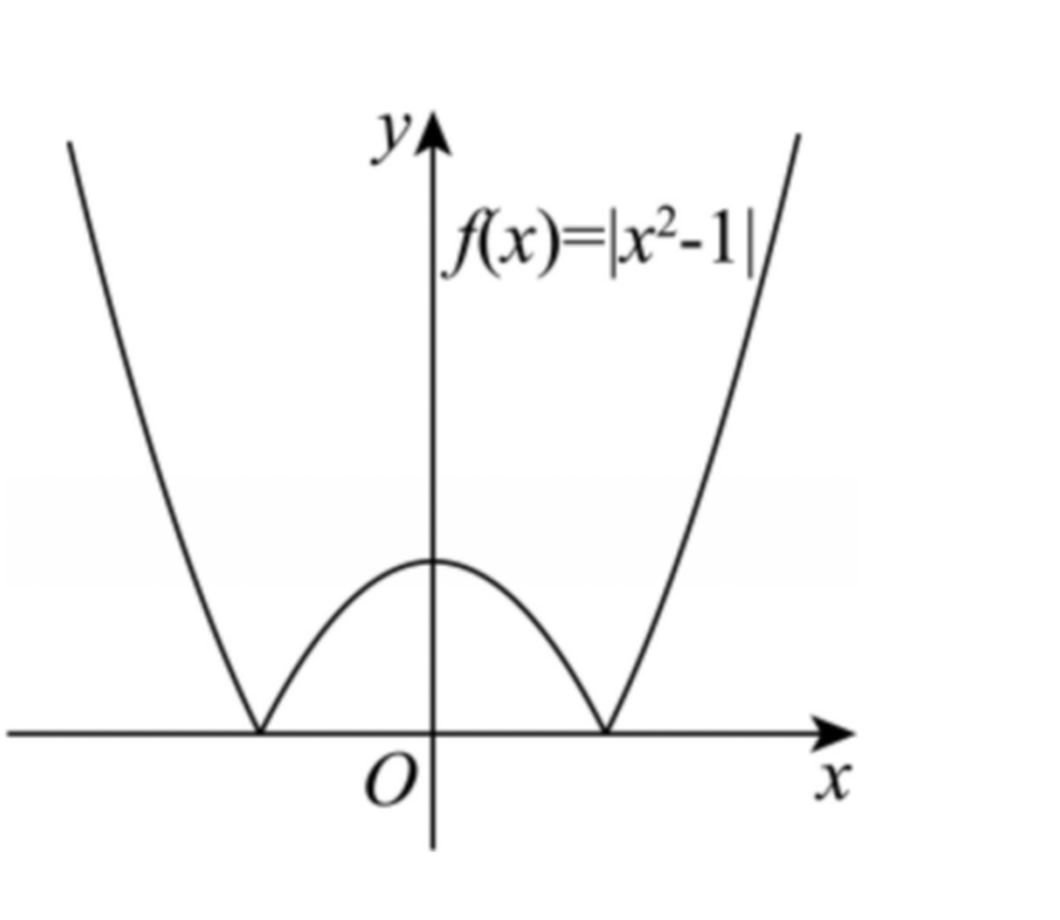
\includegraphics[width=0.40\textwidth]{figures/gao123_q20.png}
\end{center}
\step{$t=0$ 或 $t>1$ 时，每一个 $t$ 值对应 $2$ 个不同的 $x$ 值，}
\step{$t=1$ 时一个 $t$ 值对应 $3$ 个不同的 $x$ 值，}
\step{$0<t<1$ 时一个 $t$ 值对应 $4$ 个不同的 $x$ 值，}
\step{要使原方程有四个不等实根，}
\step{①$(*)$ 式一根为零，另一根大于 $1$，无解；}
\step{②$(*)$ 有两不等根且两根均大于 $1$，则 $\begin{cases}\Delta>0\\t_{\text{对}}=k>1\\f(1)>0\end{cases}$，解得 $\dfrac{1+\sqrt5}{2}<k<2$；}
\step{④$(*)$ 式有 $1$ 实根在 $(0,1)$ 之间，另一根小于零，}% 原卷由 ② 直接跳到 ④，缺 ③，照录
\step{则 $\begin{cases}f(0)<0\\f(1)>0\end{cases}$，所以 $\begin{cases}k+1<0\\2-k>0\end{cases}$，解得 $k<-1$，}
\step{综上所述，$k$ 取值范围为 $(-\infty,-1)\cup\left(\dfrac{1+\sqrt5}{2},2\right)$；}
\step{(3) 因为 $\dfrac1{a+2b}+\dfrac1{a+3}=\dfrac{a+2b+a+3}{(a+2b)(a+3)}=\dfrac{2(a+b)+3}{(a+2b)(a+3)}=\dfrac12$，}
\step{所以 $2(a+b)+3=\dfrac12(a+2b)(a+3)$，}
\step{因为 $a$、$b$ 为正实数，所以 $\dfrac12=\dfrac1{a+2b}+\dfrac1{a+3}\geqslant2\sqrt{\dfrac1{a+2b}\times\dfrac1{a+3}}$，}
\step{得 $\dfrac1{16}\geqslant\dfrac1{a+2b}\times\dfrac1{a+3}$，即 $(a+2b)(a+3)\geqslant16$，}
\step{所以 $2(a+b)+3\geqslant8$，即 $a+b\geqslant\dfrac52$，}
\step{当且仅当 $\dfrac1{a+2b}=\dfrac1{a+3}$ 即 $a=1$,$b=\dfrac32$ 时取等号，}
\step{故 $k\geqslant\dfrac52$，此时有 $\begin{cases}\Delta>0\\t_{\text{对}}=k>1\\f(0)>0,f(1)<0\end{cases}$，}
\step{故 $(*)$ 式有两不等实根且一根在 $(0,1)$ 之间，另一根大于 $1$，}
\step{故原方程有 $6$ 个实根.}
\solend
\fi

\item 设 $n$ 是不小于 $3$ 的正整数，集合 $S_n=\{(a_1,a_2,\cdots,a_n)\mid a_i\in\{0,1\},i=1,2,\cdots,n\}$，对于集合 $S_n$ 中任意两个元素 $A=(a_1,a_2,\cdots,a_n)$，$B=(b_1,b_2,\cdots,b_n)$.

定义 1：$A\cdot B=n-(\lvert a_1-b_1\rvert+\lvert a_2-b_2\rvert+\cdots+\lvert a_n-b_n\rvert)$，

定义 2：若 $A\cdot B=0$，则称互为相反元素，记作 $A=\overline B$ 或 $B=\overline A$.

(1) 若 $n=3$，$A=(0,1,0)$，$B=(1,1,0)$，试写出 $\overline A$、$\overline B$ 以及 $A\cdot B$ 的值；

(2) 若 $A$、$B\in S_n$，$A=(a_1,a_2,\cdots,a_n)$，$B=(b_1,b_2,\cdots,b_n)$，证明：$A\cdot B+\overline A\cdot B=n$；

(3) 设 $k$ 是小于 $n$ 的正奇数，至少含有两个元素的集合 $M\subseteq S_n$，且对于集合 $M$ 中任意两个不相同的元素 $A=(a_1,a_2,\cdots,a_n)$，$B=(b_1,b_2,\cdots,b_n)$，都有 $A\cdot B=n-k$，试求集合 $M$ 中元素个数的所有可能值.

\ifanswer
\solbegin
\step{(1) $\overline A=(1,0,1)$,$\overline B=(0,0,1)$,$\overline A\cdot\overline B=2$；}
\step{(2) 设 $A=(a_1,a_2,\cdots,a_n)$,$B=(b_1,b_2,\cdots,b_n)$,$\overline A=(x_1,x_2,\cdots,x_n)$，}
\step{由 $a_i$、$b_i$、$x_i\in\{0,1\}$，$i=1,2,\cdots,n$，得 $\lvert a_i-x_i\rvert\leqslant1$，$i=1,2,\cdots,n$，}
\step{所以 $\lvert a_1-x_1\rvert+\lvert a_2-x_2\rvert+\cdots+\lvert a_i-x_i\rvert\leqslant n$，}% 原卷末项下标作 $i$，照录
\step{当且仅当 $\lvert a_i-x_i\rvert=1$，$i=1,2,\cdots,n$，}
\step{即 $x_i=1-a_i$，$i=1,2,\cdots,n$ 时取等号.}
\step{由题意得 $A\cdot\overline A=n-(\lvert a_1-x_1\rvert+\lvert a_2-x_2\rvert+\cdots+\lvert a_n-x_n\rvert)=0$，}
\step{即 $\lvert a_1-x_1\rvert+\lvert a_2-x_2\rvert+\cdots+\lvert a_n-x_n\rvert=n$，}
\step{所以 $x_i=1-a_i$，$i=1,2,\cdots,n$，}
\step{$A\cdot B+\overline A\cdot B=2n-\sum\limits_{i=1}^n[\lvert a_i-b_i\rvert+(1-a_i)-b_i]$}
\step{$=2n-\sum\limits_{i=1}^n(\lvert1-b_i\rvert+\lvert0-b_i\rvert)=2n-\sum\limits_{i=1}^n(1-b_i+b_i)=2n-n=n$；}
\step{(3) 假设 $A=(a_1,a_2,\cdots,a_n)$，$B=(b_1,b_2,\cdots,b_n)$，$C=(c_1,c_2,\cdots,c_n)$}
\step{为集合 $M$ 中的三个不相同的元素，}
\step{则 $A\cdot B=n-(\lvert a_1-b_1\rvert+\lvert a_2-b_2\rvert+\cdots+\lvert a_n-b_n\rvert)=n-k$，}
\step{即 $\lvert a_1-b_1\rvert+\lvert a_2-b_2\rvert+\cdots+\lvert a_n-b_n\rvert=k$，}
\step{又由题意得 $\lvert a_i-b_i\rvert=0$ 或 $1$，$i=1,2,\cdots,n$，}
\step{$\lvert a_1-b_1\rvert$、$\lvert a_2-b_2\rvert$、$\cdots$、$\lvert a_n-b_n\rvert$ 恰有 $k$ 个 $1$，$n-k$ 个 $0$，}
\step{设其中 $k$ 个等于 $1$ 的项以此为 $a_{m_1}-b_{m_1}$,$a_{m_2}-b_{m_2}$,$\cdots$,$a_{m_k}-b_{m_k}$，}
\step{$n-k$ 个等于 $0$ 的项为 $a_{m_{k+1}}-b_{m_{k+1}}$,$a_{m_{k+2}}-b_{m_{k+2}}$,$\cdots$,$a_{m_n}-b_{m_n}$，}
\step{由题意得 $A\cdot C=n-(\lvert a_1-c_1\rvert+\lvert a_2-c_2\rvert+\cdots+\lvert a_n-c_n\rvert)=n-k$，}
\step{所以 $\sum\limits_{i=1}^k\lvert a_{m_i}-c_{m_i}\rvert+\sum\limits_{j=k+1}^n\lvert a_{m_j}-c_{m_j}\rvert=k$ ①，}
\step{同理 $\sum\limits_{i=1}^k\lvert b_{m_i}-c_{m_i}\rvert+\sum\limits_{j=k+1}^n\lvert b_{m_j}-c_{m_j}\rvert=k$ ②，}
\step{因为 $\lvert a_{m_{k+1}}-b_{m_{k+1}}\rvert=\lvert a_{m_{k+2}}-b_{m_{k+2}}\rvert=\cdots=\lvert a_{m_n}-b_{m_n}\rvert=0$，}
\step{所以 $\sum\limits_{j=k+1}^n\lvert a_{m_j}-c_{m_j}\rvert=\sum\limits_{j=k+1}^n\lvert b_{m_j}-c_{m_j}\rvert$，}
\step{由①$-$②得 $\sum\limits_{i=1}^k(\lvert a_{m_i}-c_{m_i}\rvert-\lvert b_{m_i}-c_{m_i}\rvert)=0$，}
\step{又 $\sum\limits_{i=1}^k(\lvert a_{m_i}-c_{m_i}\rvert-\lvert b_{m_i}-c_{m_i}\rvert)=\sum\limits_{i=1}^k(\lvert1-c_{m_i}\rvert-\lvert0-c_{m_i}\rvert)=k-2\sum\limits_{i=1}^k c_{m_i}$}
\step{为奇数，与 $\sum\limits_{i=1}^k(\lvert a_{m_i}-c_{m_i}\rvert-\lvert b_{m_i}-c_{m_i}\rvert)=0$ 矛盾，所以假设不成立，}
\step{即集合 $M$ 中至多有两个元素，}
\step{当 $M=\{(1,1,\cdots,1,0,0,\cdots,0),(0,0,\cdots,0)\}$ 时符合题意，}
\step{所以集合 $M$ 中元素的个数只可能是 $2$.}
\solend
\fi

\end{enumerate}

\end{document}
"
%
% 原始材料：微信公众号“魔都数学加油站”文章，作者破晓，2026-11-09 17:52 发布；
% 连载“27学年高一123”，原文标题“27学年高一123——2026-2027年上海市行知中学高一上10月月考”；
% 原文链接：https://mp.weixin.qq.com/s/GV4SWBLUJrBhMQwo22FVzg。
% 正文为 14 张 PNG 页（第 7、9、11、13、14 页 2560×3620，其余 4762×6735），
% 题目下印有【答案】或【解析】，为讲评版。
% 题目、解析均据原图转录；卷面红色水印及公众号页脚未录入。
% 全卷 3 张插图：第 5 题的坐标示意图、第 17 题的文氏图（均属题干，三版都出）、
% 第 20 题 (2) 的 $t=\lvert x^2-1\rvert$ 图象（属解析，仅答案版出）；
% 都取原卷截图去水印、2× LANCZOS 放大，见 figures/gao123_q5.png、
% figures/gao123_q17.png、figures/gao123_q20.png。
%
% 卷首标题：原卷印作“2026-2027 年行知中学高一上 10 月月考”（公众号标题中的“上海市”
% 卷面标题行没有，本稿照卷面），年份区间按全稿惯例排 en dash；原卷未印副标题，本稿按题目内容
% 标为“集合与常用逻辑用语、不等式”（与 110／111／113／116／118／120 同）。
%
% 与原卷的排版差异：
%   ① 原文从第 3 题起，填空题编号为 3—12、选择题为 13—16、解答题为 17—21，本稿保留原题号；
%   ② 原卷每题下直接印【解析】／【答案】，本稿按全稿惯例置于答案版；第 3 题只印【答案】、
%      另提 \ans{}；选择题答案在解析末句“故选 …”，括号内留空；
%   ③ 原卷未印副标题，本稿按“知识模块”口径补出；
%   ④ 原卷填空横线按全稿惯例排为 \blankline[4.4em]；选择题括号排 \mbox{（\quad）}、
%      选项段前按惯例加 \keepwithprev；解答题不留作答区（原卷为讲评版，与 109—122 同）；
%   ⑤ 原卷数集排斜体 $R$／$Z$（第 9 题作粗体 $\mathbf{R}$），按全稿惯例改 \R／\Z；
%      绝对值按全稿惯例排 \lvert…\rvert，集合描述竖线排 \mid；单位 km、h 原卷排斜体，
%      本稿按正体照排；补集照原卷上划线排 \overline{B}、\overline{A}。
%
% 判别式与子集符号：第 16 题解析的 $\triangle=b^2-4c<0$、第 20 题 (1) ① 的 $\triangle<0$
%   均作等边、扁的 \triangle；第 20 题 ② 两处 cases 与 (3) 的 $\Delta\geqslant0$／$\Delta>0$
%   作等腰、高的 \Delta，逐处照录、不统一；第 15 题选项与第 17 题 (2) 的 $\subseteq$
%   印有下划线，照录 \subseteq。
%
% 原卷存疑照录：
%   第 4 题解析“若 $-\lvert a\rvert=0$，则 $a=0$，则 $A=\{0,-1,0\}$”以元素重复说明互异性；
%   第 5 题解析“当 $a^2+b^2=400^2+b^2<500^2$”等式左边 $a^2$ 与 $400^2$ 并用；
%   第 9 题解析“解得 $a>1$ 得 $a<\dfrac13$”（按平方不等式应为 $a>1$ 或 $a<\dfrac13$）；
%   第 12 题解析“所以 $-\dfrac1{2^a}\cdot\dfrac1{2^b}\geqslant-\dfrac14$”带负号起论；
%   第 17 题 (1) 解析把阴影部分（实为 $A\cap\overline B$）印作 $\overline{A\cap B}$；
%   第 18 题 (2) 解析作“$n<1$，所以 $n-1<0$”，与题设 $m<1$ 字母不一致；
%   第 20 题 (2) 的情形编号由 ①、② 直接跳到 ④（缺 ③）；
%   第 21 题 (2) 解析“$\lvert a_1-x_1\rvert+\cdots+\lvert a_i-x_i\rvert\leqslant n$”
%   末项下标作 $i$（按上下文应为 $n$）。以上均照录加注。
%
% 行数核对：逐题数 \step 条数，合计 176 条（Q3：0；Q4：6；Q5：5；Q6：5；Q7：4；
% Q8：6；Q9：5；Q10：5；Q11：10；Q12：6；Q13：9；Q14：1；Q15：5；Q16：21；
% Q17：8；Q18：14；Q19：10；Q20：26；Q21：30），与原卷印刷行逐题相等
% （cases 块作一个印刷行计）。第 3 题只印【答案】，提 \ans{}，不计入 \step 账。
%
\documentclass[a4paper,11pt]{article}
\usepackage{common}

\begin{document}

\examtitlest[3]{2026--2027 年行知中学高一上 10 月月考}{集合与常用逻辑用语、不等式}

\bigsec{一、填空题}

\begin{enumerate}
\setcounter{enumi}{2}

\item 写出命题“存在实数 $x$、$y$、$z$，使 $x<y$ 或 $y<z$.”的否定\blankline[4.4em].

\ifanswer
\ans{任意实数 $x$、$y$、$z$，使得 $x\geqslant y$ 且 $y\geqslant z$}
\fi

\item 若集合 $\{0,-1,2a\}=\{a-1,-\lvert a\rvert,a+1\}$，实数 $a$ 的值为\blankline[4.4em].

\ifanswer
\solbegin
\step{令 $A=\{0,-1,2a\}$,$B=\{a-1,-\lvert a\rvert,a+1\}$，}
\step{因为 $\{0,-1,2a\}=\{a-1,-\lvert a\rvert,a+1\}$，}
\step{若 $a-1=0$，则 $a=1$，则 $A=\{0,-1,2\}$,$B=\{0,-1,2\}$，满足要求；}
\step{若 $-\lvert a\rvert=0$，则 $a=0$，则 $A=\{0,-1,0\}$，不满足集合元素的互异性；}% 原卷以 $A=\{0,-1,0\}$ 说明互异性，照录
\step{若 $a+1=0$，则 $a=-1$，则 $A=\{0,-1,-2\}$,$B=\{0,-1,-2\}$，满足要求；}
\step{故实数 $a$ 的值为 $\pm1$.}
\solend
\fi

\needvspace{7cm}
\item 如图，据气象部门预报，在距离某码头南偏东 $45^\circ$ 方向 $400\sqrt2$ km 处的热带
风暴中心正在以 $20$km/h 的速度向正北方向移动，距风暴中心 $500$km 以内
的地区都将受到影响. 以上预报估计，该码头将受到热带风暴的影响时长大
约为\blankline[4.4em]$h$.

\begin{center}
% 图取原卷截图（第 1 页题干右侧）、去水印后 2× LANCZOS 放大，本稿移至题干之后
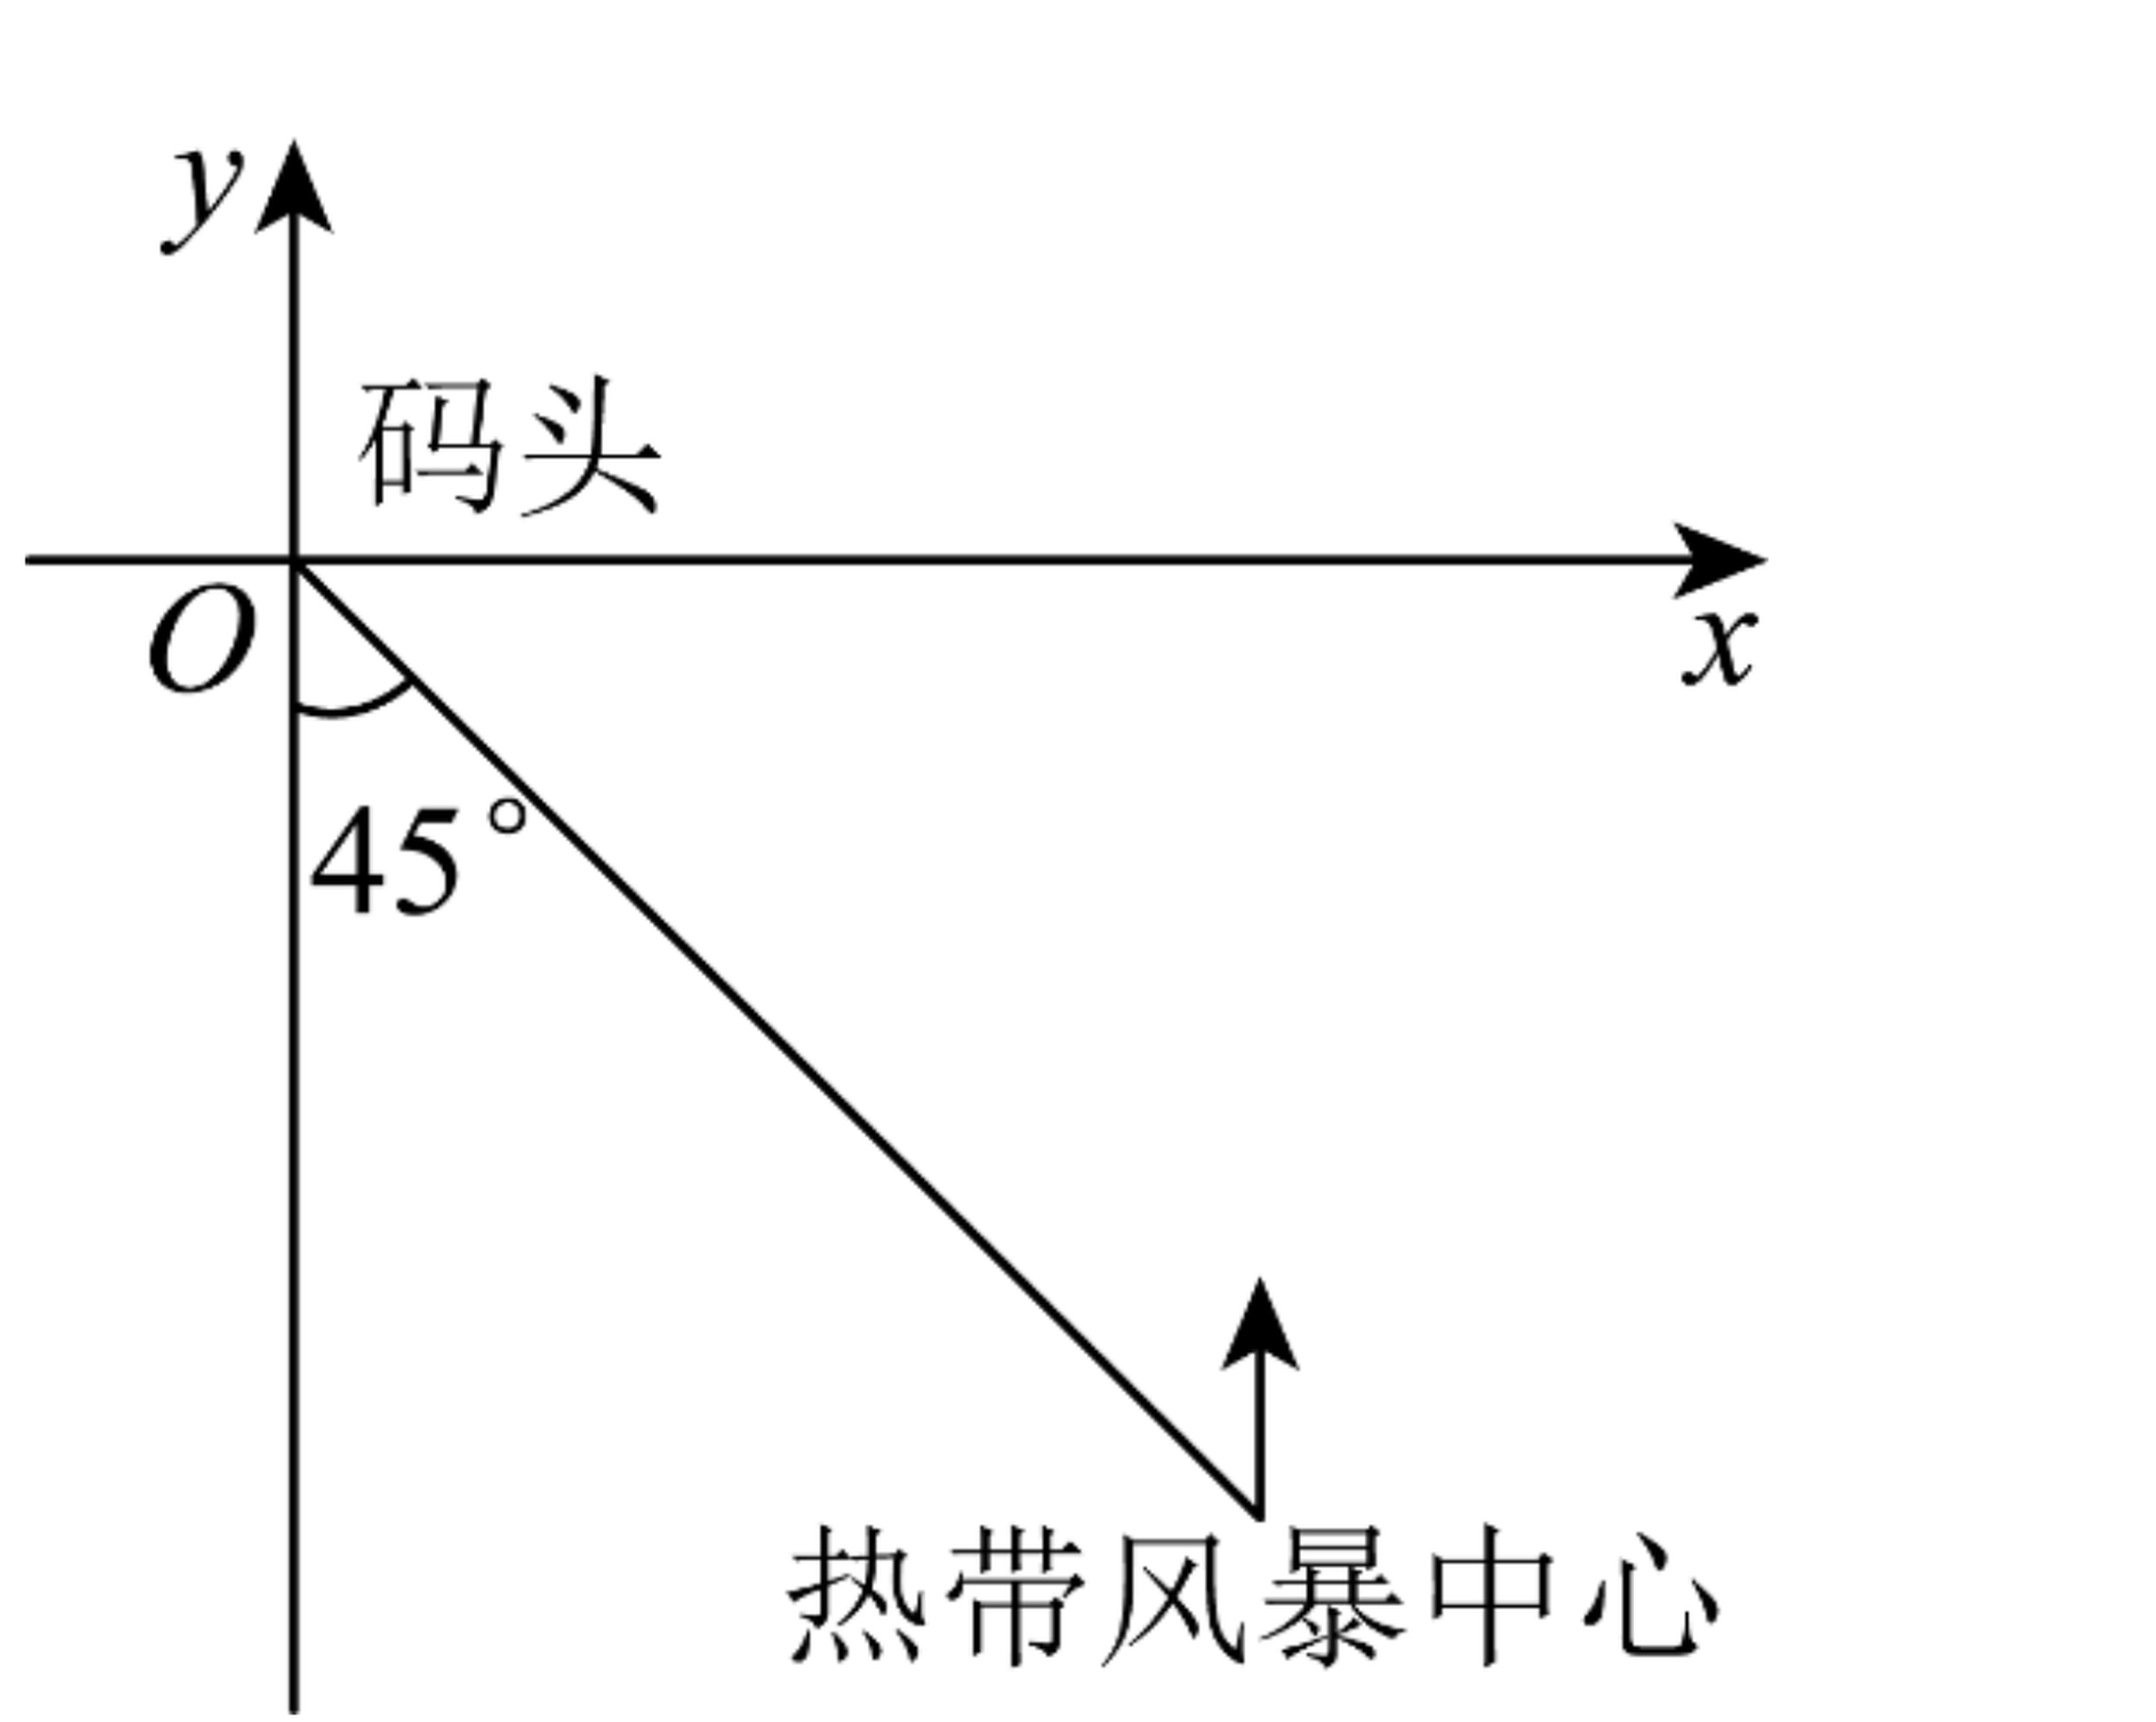
\includegraphics[width=0.36\textwidth]{figures/gao123_q5.png}
\end{center}

\ifanswer
\solbegin
\step{设风暴中心的坐标为 $(a,b)$，}
\step{由题意得 $a=400\sqrt2\times\cos45^\circ=400$，当 $a^2+b^2=400^2+b^2<500^2$，}% 原卷 $a^2$ 与 $400^2$ 并用，照录
\step{即 $-300<b<300$ 时，码头将受到风暴影响，}
\step{$\dfrac{300-(-300)}{20}=30h$，则码头受到风暴影响的时长为 30 小时，}
\step{所以由预报估计，该码头将受到热带风暴的影响时长大约为 30 小时.}
\solend
\fi

\item 已知 $a$、$b$、$c$ 为常数，若不等式 $\dfrac{ax-b}{x-c}\geqslant0$ 的解集为 $[-1,1)$，则不等式 $ax+b<0$ 的解集为\blankline[4.4em].

\ifanswer
\solbegin
\step{不等式 $\dfrac{ax-b}{x-c}\geqslant0$ 可化为 $(ax-b)(x-c)\geqslant0$ 且 $x-c\neq0$，}
\step{即 $a\left(x-\dfrac ba\right)(x-c)\geqslant0$ 且 $x\neq c$，}
\step{因为不等式 $\dfrac{ax-b}{x-c}\geqslant0$ 的解集为 $[-1,1)$，所以 $a<0$，且 $\dfrac ba=-1$,$c=1$，}
\step{即 $b=-a$，所以不等式 $ax+b<0$ 可化为 $ax-a<0$，又因为 $a<0$，所以 $x-1>0$，}
\step{解得 $x>1$，所以不等式 $ax+b<0$ 的解集为 $(1,+\infty)$.}
\solend
\fi

\item 已知实数 $a$、$b$ 满足 $ab=32$，且 $\log_2a=\log_b16$，则 $a+b$ 的值为\blankline[4.4em].

\ifanswer
\solbegin
\step{由 $\log_2a=\log_b16$，得 $\log_2a=\dfrac{\log_216}{\log_2b}$，则 $\log_2a\cdot\log_2b=4$，}
\step{由 $ab=32$，得 $\log_2a+\log_2b=\log_2ab=5$，}
\step{得 $\log_2a=1$,$\log_2b=4$ 或 $\log_2a=4$,$\log_2b=1$，}
\step{因此 $a=2$,$b=16$ 或 $a=16$,$b=2$，所以 $a+b=18$.}
\solend
\fi

\item 已知实数 $a$、$b$ 满足 $-3<a+2b<2$，$-1<2a-b<4$，则 $a+b$ 的取值范围为\blankline[4.4em].

\ifanswer
\solbegin
\step{设 $a+b=m(a+2b)+n(2a-b)=(m+2n)a+(2m-n)b$，}
\step{所以 $\begin{cases}m+2n=1\\2m-n=1\end{cases}$，解得 $n=\dfrac15$,$m=\dfrac35$，所以 $a+b=\dfrac35(a+2b)+\dfrac15(2a-b)$，}
\step{因为 $-3<(a+2b)<2$，$-1<2a-b<4$，}
\step{所以 $-\dfrac95<\dfrac35(a+2b)<\dfrac65$，$-\dfrac15<\dfrac15(2a-b)<\dfrac45$，}
\step{相加得 $-2<\dfrac35(a+2b)+\dfrac15(2a-b)<2$，即 $-2<a+b<2$，}
\step{故 $a+b$ 的取值范围为 $(-2,2)$.}
\solend
\fi

\item 存在 $x\in\R$ 使不等式 $\lvert2x-a\rvert<\lvert2a-1\rvert-2\lvert x\rvert$ 成立，则实数 $a$ 的取值范围是\blankline[4.4em].

\ifanswer
\solbegin
\step{存在 $x\in\R$，不等式 $\lvert2x-a\rvert<\lvert2a-1\rvert-2\lvert x\rvert$ 成立，}
\step{变形即 $\lvert2x-a\rvert+2\lvert x\rvert<\lvert2a-1\rvert$ 成立，}
\step{由于 $\lvert2x-a\rvert+\lvert2x\rvert\geqslant\lvert(2x-a)-2x\rvert=\lvert a\rvert$，当且仅当 $2x(2x-a)\leqslant0$ 时取等号，}
\step{因此有 $\lvert a\rvert<\lvert2a-1\rvert$，两边平方 $a^2<(2a-1)^2$，解得 $a>1$ 得 $a<\dfrac13$，}% 原卷“解得 a>1 得 a<1/3”，照录
\step{即实数 $a$ 的取值范围是 $\left(-\infty,\dfrac13\right)\cup(1,+\infty)$.}
\solend
\fi

\item 已知集合 $A=\{(x,y)\mid x^2+mx-y+2=0\}$，$B=\{(x,y)\mid x-y+1=0,0\leqslant x\leqslant3\}$，若集合 $A\cap B$ 的子集个数为 $2$，则实数 $m$ 的取值范围为\blankline[4.4em].

\ifanswer
\solbegin
\step{因为集合 $A\cap B$ 的子集个数为 $2$，所以 $A\cap B$ 的元素有一个，}
\step{即 $\begin{cases}x^2+mx-y+2=0\\x-y+1=0\end{cases}$ 在 $x\in[0,3]$ 上只有一个解，}
\step{即 $x^2+(m-1)x+1=0$ 在 $[0,3]$ 上只有一个解，}
\step{即 $1-m=x+\dfrac1x$ 在 $[0,3]$ 上只有一个解，}
\step{结合对勾函数的性质得 $1-m=2$ 或 $1-m>\dfrac{10}{3}$，解得 $m=-1$ 或 $m<-\dfrac73$.}
\solend
\fi

\item $[x]$ 表示不超过 $x$ 的最大整数，则集合 $A=\left\{y\,\middle\vert\,y=\left[\dfrac{x^2}{100}\right],x=1,2,3,\cdots,100\right\}$ 中的元素个数为\blankline[4.4em].

\ifanswer
\solbegin
\step{记 $a_k=\left[\dfrac{k^2}{100}\right](k=1,2,\cdots,100)$，$a_k$ 随 $k$ 增大而单调不减.}
\step{当 $k\geqslant50$ 时，$\dfrac{(k+1)^2}{100}-\dfrac{k^2}{100}=\dfrac{2k+1}{100}\geqslant\dfrac{101}{100}>1$，所以 $a_{k+1}\geqslant a_k+1$，}
\step{即 $a_{50}$、$a_{51}$、$\cdots$、$a_{100}$ 两两互异.}
\step{又 $a_{50}=\left[\dfrac{2500}{100}\right]=25$、$a_{100}=100$，这一段共 $100-50+1=51$ 个互异的值，}
\step{且都大于等于 $25$.}
\step{当 $k\leqslant49$ 时，$\dfrac{(k+1)^2}{100}-\dfrac{k^2}{100}=\dfrac{2k+1}{100}\leqslant\dfrac{99}{100}<1$，即 $a_k$ 每次至多增加 $1$；}
\step{又 $a_1=0$、$a_{49}=\left[\dfrac{2401}{100}\right]=24$，}
\step{故 $a_1$、$a_2$、$\cdots$、$a_{49}$ 依次取遍 $0$，$1$，$2$，$\cdots$，$24$，共 $25$ 个值.}
\step{两段取值范围互不重叠（前段不超过 $24$、后段不小于 $25$），}
\step{所以集合 $A$ 中共有 $25+51=76$ 个元素.}
\solend
\fi

\item 若实数 $a$、$b$、$c$ 满足 $\dfrac1{2^a}+\dfrac1{2^b}=1$，$\dfrac1{2^{a+b}}+\dfrac1{2^{b+c}}+\dfrac1{2^{a+c}}=1$，则 $c$ 的最大值是\blankline[4.4em].

\ifanswer
\solbegin
\step{因为 $\dfrac1{2^a}+\dfrac1{2^b}=1$，}
\step{由基本不等式得 $1=\dfrac1{2^a}+\dfrac1{2^b}\geqslant2\sqrt{\dfrac1{2^a}\cdot\dfrac1{2^b}}$（当且仅当 $a=b=1$ 时取等号），}
\step{所以 $\dfrac1{2^a}\cdot\dfrac1{2^b}\leqslant\dfrac14$，所以 $-\dfrac1{2^a}\cdot\dfrac1{2^b}\geqslant-\dfrac14$，}% 原卷带负号起论，照录
\step{因为 $\dfrac1{2^{a+b}}+\dfrac1{2^{b+c}}+\dfrac1{2^{a+c}}=1$，$\dfrac1{2^{b+c}}+\dfrac1{2^{a+c}}=\dfrac1{2^c}\left(\dfrac1{2^a}+\dfrac1{2^b}\right)=\dfrac1{2^c}$，}
\step{所以 $\dfrac1{2^c}=1-\dfrac1{2^{a+b}}\geqslant\dfrac34$，所以 $2^c\leqslant\dfrac43$，所以 $c\leqslant\log_2\dfrac43=2-\log_23$，}
\step{故 $c$ 的最大值是 $2-\log_23$.}
\solend
\fi

\end{enumerate}

\bigsec{二、选择题}

\begin{enumerate}
\setcounter{enumi}{12}

\item 下列运用等式或不等式的性质变形中，正确的是\mbox{（\quad）}

\keepwithprev
A. 如果 $a=b$，那么 $\dfrac ac=\dfrac bc$\qquad\qquad B. 如果 $\dfrac1a<\dfrac1b<0$，那么 $a-\dfrac1a>b-\dfrac1b$

C. 如果 $a>b$，那么 $\dfrac1a<\dfrac1b$\qquad\qquad D. 如果 $a>b>0$，$m\in\R$，那么 $\dfrac ba<\dfrac{b+m}{a+m}$

\ifanswer
\solbegin
\step{对于 $A$，若 $c=0$，$A$ 错误；}
\step{对于 $B$，若 $\dfrac1a<\dfrac1b<0$，则 $0>a>b$，$-\dfrac1a>-\dfrac1b>0$，}
\step{所以 $a-\dfrac1a>b-\dfrac1b$，$B$ 正确；}
\step{对于 $C$，$a>0$，$b<0$ 时，$C$ 错误；}
\step{对于 $D$，$\dfrac{b+m}{a+m}-\dfrac ba=\dfrac{ab+am}{a(a+m)}-\dfrac{ab+bm}{a(a+m)}=\dfrac{(a-b)m}{a(a+m)}$，}
\step{因为 $a>b>0$，所以 $a-b>0$，但 $m$、$a+m$ 的符号不确定，}
\step{当 $m=0$ 时，$\dfrac ba=\dfrac{b+m}{a+m}$，}
\step{当 $m(a+m)>0$ 时，$\dfrac ba<\dfrac{b+m}{a+m}$，当 $m(a+m)<0$ 时，$\dfrac ba>\dfrac{b+m}{a+m}$，$D$ 错误.}
\step{故选 $B$.}
\solend
\fi

\item “$a>b$”的一个必要非充分条件是\mbox{（\quad）}

\keepwithprev
A. $ac^2>bc^2$\qquad\quad B. $2^a>2^b$\qquad\quad C. $\left(\dfrac12\right)^{a-b}\leqslant1$\qquad\quad D. $a^3>b^3$

\ifanswer
\solbegin
\step{即“$a>b$”能推出选项，但选项不能推出“$a>b$”，故选 $C$.}
\solend
\fi

\item 若 $A=\left\{x\,\middle\vert\,x=\dfrac k6+1,k\in\Z\right\}$，$B=\left\{x\,\middle\vert\,x=\dfrac k3+\dfrac12,k\in\Z\right\}$，$C=\left\{x\,\middle\vert\,x=\dfrac{2k}{3}+\dfrac12,k\in\Z\right\}$，则这三个集合间的关系是\mbox{（\quad）}

\keepwithprev
A. $A\subseteq B\subseteq C$\qquad\quad B. $A\subseteq C\subseteq B$\qquad\quad C. $C\subseteq B\subseteq A$\qquad\quad D. $C\subseteq A\subseteq B$

\ifanswer
\solbegin
\step{若 $x\in C$，则存在 $k_0\in\Z$，使 $x=\dfrac{2k_0}{3}+\dfrac12$，}
\step{又 $2k_0\in\Z$，所以 $x\in B$，故 $C\subseteq B$，}
\step{若 $x\in B$，则存在 $k_1\in\Z$，使 $x=\dfrac{k_1}{3}+\dfrac12=\dfrac{2k_1-3}{6}+1$，}
\step{又 $2k_1-3\in\Z$，所以 $x\in A$，故 $B\subseteq A$，}
\step{又 $\dfrac43\in A$，$\dfrac43\notin B$，$\dfrac56\in B$，$\dfrac56\notin C$，所以 $C\subseteq B\subseteq A$，故选 $C$.}
\solend
\fi

\item 集合 $S=\{x\mid(x+a)(x^2+bx+c)=0\}$，$T=\{x\mid(ax+1)(cx^2+bx+1)=0\}$，其中 $a$、$b$、$c$ 为实数，若 $\lvert S\rvert$、$\lvert T\rvert$ 分别表示 $S$、$T$ 的元素个数，则下列结论中一定成立的是\mbox{（\quad）}

\keepwithprev
A. 若 $\lvert T\rvert=0$，则 $\lvert S\rvert=1$\qquad\qquad B. 若 $\lvert S\rvert=1$，则 $\lvert T\rvert=1$

C. 若 $\lvert S\rvert=2$，则 $\lvert T\rvert=2$\qquad\qquad D. 若 $\lvert T\rvert=3$，则 $\lvert S\rvert=2$

\ifanswer
\solbegin
\step{令 $f(x)=(x+a)(x^2+bx+c)$,$g(x)=(ax+1)(cx^2+bx+1)$，}
\step{对于选项 A，当 $\lvert T\rvert=0$ 时，方程 $g(x)=(ax+1)(cx^2+bx+1)=0$ 无实根，}
\step{当 $a=b=c=0$ 时，$f(x)=x^3$，由 $f(x)=0$ 得 $x=0$，此时 $\lvert S\rvert=1$；}
\step{当 $a=0$,$b^2-4c<0$ 时，$f(x)=x(x^2+bx+c)$，由 $f(x)=0$ 得 $x=0$，}
\step{此时 $\lvert S\rvert=1$，所以选项 A 正确；}
\step{对于选项 B，若 $\lvert S\rvert=1$，则 $f(x)=(x+a)(x^2+bx+c)=0$ 有且只有一根，}
\step{又 $x=-a$ 一定是 $f(x)=0$ 的根，所以 $\triangle=b^2-4c<0$，}
\step{又 $\triangle=b^2-4c<0$ 且 $a=0$ 时，$g(x)=(ax+1)(cx^2+bx+1)=0$ 无解，}
\step{此时 $\lvert T\rvert=0$，所以选项 B 错误，}
\step{对于选项 C，若 $\lvert S\rvert=2$ 时，则 $f(x)=(x+a)(x^2+bx+c)=0$ 有且只有 $2$ 根，}
\step{又 $x=-a$ 一定是 $f(x)=0$ 的根，}
\step{所以 $\triangle=b^2-4c=0$ 且 $a^2+ab+c\neq0$ 或 $\triangle=b^2-4c>0$ 且 $a^2+ab+c=0$，}
\step{当 $a=0$ 时，存在 $b$,$c$，使 $\triangle=b^2-4c=0$ 且 $a^2+ab+c\neq0$，}
\step{此时 $g(x)=(ax+1)(cx^2+bx+1)=0$ 只有一根，所以选项 C 错误，}
\step{对于选项 D，当 $\lvert T\rvert=3$ 时，方程 $g(x)=(ax+1)(cx^2+bx+1)=0$ 有三个根，}
\step{所以 $a\neq0$,$c\neq0$,$b^2-4c>0$，}
\step{设 $x_0$ 为 $g(x)=0$ 的一个根，即 $(ax_0+1)(cx_0^2+bx_0+1)=0$，}
\step{则 $x_0\neq0$，且 $f\left(\dfrac1{x_0}\right)=\left(\dfrac1{x_0}+a\right)\left(\dfrac1{x_0^2}+\dfrac1{x_0}b+c\right)=\dfrac1{x_0^3}g(x_0)=0$，}
\step{所以 $\dfrac1{x_0}$ 为方程 $f(x)=0$ 的根，故 $f(x)=0$ 有三个根，即 $\lvert T\rvert=3$ 时，}
\step{必有 $\lvert S\rvert=3$，所以选项 D 错误，}
\step{故选 $A$.}
\solend
\fi

\end{enumerate}

% 第 17 题是解答题第一题且带文氏图，守卫放在 \bigsec 之前，连节标题一起量页高
\needvspace{7cm}
\bigsec{三、解答题}

\begin{enumerate}
\setcounter{enumi}{16}

\item 设全集 $U=\R$，集合 $A=\{x\mid-2\leqslant x\leqslant4\}$，$B=\{x\mid x<-6$ 或 $x\geqslant2\}$.

（1）求图中阴影部分表示的集合；

（2）已知集合 $C=\{x\mid10-a<x<2a+1\}$，若 $\overline B\cap C=\varnothing$，求 $a$ 的取值范围.

\begin{center}
% 图取原卷截图（第 7 页题干右侧）、去水印后 2× LANCZOS 放大，本稿移至题干之后
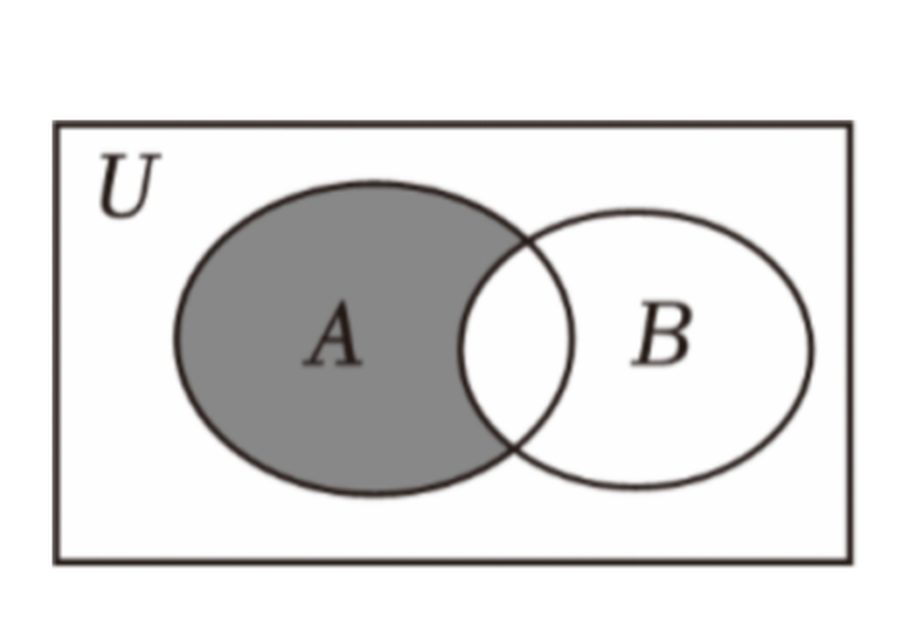
\includegraphics[width=0.34\textwidth]{figures/gao123_q17.png}
\end{center}

\ifanswer
\solbegin
\step{（1）$A\cap B=\{x\mid2\leqslant x\leqslant4\}$，}
\step{则图中阴影部分表示 $\overline{A\cap B}=\{x\mid-2\leqslant x<2\}$.}% 原卷把上划线盖在整个 $A\cap B$ 上，照录
\step{（2）由题意得 $\overline B=\{x\mid-6\leqslant x<2\}$，$C\subseteq B$，}
\step{所以当 $C=\varnothing$ 时，$10-a\geqslant2a+1$，解得 $a\leqslant3$，符合题意；}
\step{当 $C\neq\varnothing$ 时，$\begin{cases}10-a<2a+1\\2a+1\leqslant-6\end{cases}$ 或者 $\begin{cases}10-a<2a+1\\10-a\geqslant2\end{cases}$，}
\step{此时不等式组 $\begin{cases}10-a<2a+1\\2a+1\leqslant-6\end{cases}$ 无解，}
\step{不等式组 $\begin{cases}10-a<2a+1\\10-a\geqslant2\end{cases}$ 的解集为 $3<a\leqslant8$，}
\step{综上，$a$ 的取值范围为 $\{a\mid a\leqslant8\}$.}
\solend
\fi

\item (1) 求不等式：$\lvert x-1\rvert+\lvert x-2\rvert\leqslant5$ 的解集.

(2) 当 $m<1$ 时，解关于 $x$ 的不等式 $\dfrac{m(x-3)}{x+2}>1$.

\ifanswer
\solbegin
\step{(1) 当 $x<1$ 时，$\lvert x-1\rvert+\lvert x-2\rvert\leqslant5\Leftrightarrow-x+1+2-x\leqslant5$，}
\step{解得 $-1\leqslant x<1$；}
\step{当 $1\leqslant x\leqslant2$ 时，$\lvert x-1\rvert+\lvert x-2\rvert\leqslant5\Leftrightarrow x-1+2-x=1\leqslant5$ 恒成立，}
\step{所以 $1\leqslant x\leqslant2$；}
\step{当 $x>2$ 时，$\lvert x-1\rvert+\lvert x-2\rvert\leqslant5\Leftrightarrow x-1+x-2=2x-3\leqslant5$，}
\step{解得 $2<x\leqslant4$.}
\step{综上所述，不等式 $\lvert x-1\rvert+\lvert x-2\rvert\leqslant5$ 的解集为 $[-1,4]$.}
\step{(2) 原不等式变成 $\dfrac{(m-1)x-(3m+2)}{x+2}>0$，$n<1$，所以 $n-1<0$，}% 原卷作 $n<1$、$n-1<0$，与题设 $m<1$ 字母不一致，照录
\step{所以原不等式变成 $\dfrac{x-\dfrac{3m+2}{m-1}}{x+2}<0$，$\dfrac{3m+2}{m-1}-(-2)=\dfrac{5m}{m-1}$，}
\step{所以 $m<0$ 时，$\dfrac{5m}{m-1}>0$，$\dfrac{3m+2}{m-1}>-2$，}
\step{原不等式的解集为 $\left(-2,\dfrac{3m+2}{m-1}\right)$；}
\step{$m=0$ 时，原不等式变成 $1<0$，无解；}
\step{$0<m<1$ 时，$\dfrac{5m}{m-1}<0$，$\dfrac{3m+2}{m-1}<-2$，}
\step{原不等式的解集为 $\left(\dfrac{3m+2}{m-1},-2\right)$.}
\solend
\fi

\item 在园林博览会上，某公司带来了一种智能设备供采购商洽谈采购，并决定大量投放市场，已知该种设备年固定研发成本为 $50$ 万元，每生产一台需另投入 $100$ 元，设该公司一年内生产该设备 $x$ 万台且全部售完，每万台的销售收入 $G(x)$（万元）与年产量 $x$（万台）满足如下关系式：$G(x)=\begin{cases}180-x,0<x\leqslant20\\80+\dfrac{2000}{x}-\dfrac{8000}{x(x-1)},x>20\end{cases}$.

(1) 写出年利润 $W(x)$（万元）关于年产量 $x$（万台）的函数解析式；（利润 $=$ 销售收入 $-$ 成本）

(2) 当年产量为多少万台时，该公司获得的年利润最大，并求出最大利润.

\ifanswer
\solbegin
\step{(1) $W(x)=xG(x)-50-100x=\begin{cases}-50+80x-x^2,0<x\leqslant20\\-20x+1950-\dfrac{8000}{x-1},x>20\end{cases}$；}
\step{(2) 当 $0<x\leqslant20$ 时，$W(x)=-50+80x-x^2=-(x-40)^2+1550$，}
\step{由函数性质得当 $x\leqslant40$ 时严格增，所以当 $x=20$ 时，$W(x)_{max}=1150$，}
\step{当 $x>20$ 时，$W(x)=-20x+1950-\dfrac{8000}{x-1}=-20\left[(x-1)+\dfrac{400}{x-1}\right]+1930$，}
\step{$W(x)=-20\left[(x-1)+\dfrac{400}{x-1}\right]+1930\leqslant-20\times2\sqrt{(x-1)\cdot\dfrac{400}{x-1}}+1930$}
\step{$=1130$，当且仅当 $x-1=\dfrac{400}{x-1}$，即 $x=21$ 时取等号，}
\step{所以 $W(x)_{max}=1130$，}
\step{因为 $1150>1130$，所以当 $x=20$ 时，$W(x)_{max}=1150$，}
\step{即当年产量为 $20$ 万台时，该公司获得的年利润最大，}
\step{最大利润为 $1150$ 万元.}
\solend
\fi

\item 关于 $x$ 的方程 $(x^2-1)^2-2k\lvert x^2-1\rvert+k+1=0(k\in\R)$.

(1) 若方程无实根，求 $k$ 的取值范围；

(2) 若方程有 $4$ 个不等实根，求 $k$ 的取值范围；

(3) 若 $k=a+b$，且满足 $\dfrac1{a+2b}+\dfrac1{a+3}=\dfrac12$，$a>0$，$b>0$，试判断方程根的个数.

\ifanswer
\solbegin
\step{(1) 关于 $x$ 的方程 $(x^2-1)^2-2k\lvert x^2-1\rvert+k+1=0(k\in\R)$，}
\step{令 $t=\lvert x^2-1\rvert$，则 $t\geqslant0$，则原方程转化为 $t^2-2kt+k+1=0(*)$，}
\step{因为关于 $x$ 的方程 $(x^2-1)^2-2k\lvert x^2-1\rvert+k+1=0(k\in\R)$ 无实根，}
\step{所以 $(*)$ 式无实根或实根均小于零，令 $f(t)=t^2-2kt+k+1$，}
\step{①若 $(*)$ 式无实根，则 $\triangle<0$，解得 $\dfrac{1-\sqrt5}{2}<k<\dfrac{1+\sqrt5}{2}$，}
\step{②两根均为负，则 $\begin{cases}\Delta\geqslant0\\t_{\text{对}}=k<0\\f(0)>0\end{cases}$，解得 $-1<k\leqslant\dfrac{1-\sqrt5}{2}$，}
\step{综合①②，得 $k$ 的取值范围是 $\left(-1,\dfrac{1+\sqrt5}{2}\right)$；}
\step{(2) 作函数 $t=\lvert x^2-1\rvert$ 的图象，}
\begin{center}
% 图取原卷截图（第 11 页解析内）、去水印后 2× LANCZOS 放大，仅答案版出
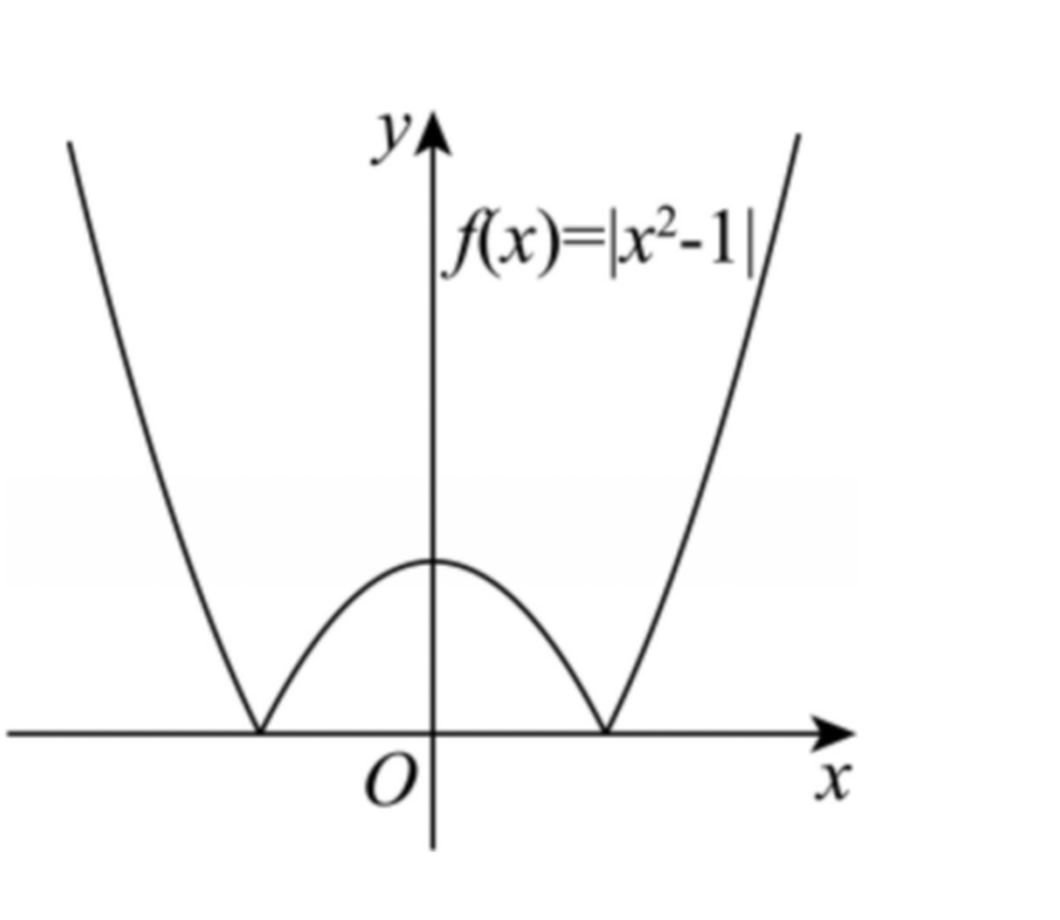
\includegraphics[width=0.40\textwidth]{figures/gao123_q20.png}
\end{center}
\step{$t=0$ 或 $t>1$ 时，每一个 $t$ 值对应 $2$ 个不同的 $x$ 值，}
\step{$t=1$ 时一个 $t$ 值对应 $3$ 个不同的 $x$ 值，}
\step{$0<t<1$ 时一个 $t$ 值对应 $4$ 个不同的 $x$ 值，}
\step{要使原方程有四个不等实根，}
\step{①$(*)$ 式一根为零，另一根大于 $1$，无解；}
\step{②$(*)$ 有两不等根且两根均大于 $1$，则 $\begin{cases}\Delta>0\\t_{\text{对}}=k>1\\f(1)>0\end{cases}$，解得 $\dfrac{1+\sqrt5}{2}<k<2$；}
\step{④$(*)$ 式有 $1$ 实根在 $(0,1)$ 之间，另一根小于零，}% 原卷由 ② 直接跳到 ④，缺 ③，照录
\step{则 $\begin{cases}f(0)<0\\f(1)>0\end{cases}$，所以 $\begin{cases}k+1<0\\2-k>0\end{cases}$，解得 $k<-1$，}
\step{综上所述，$k$ 取值范围为 $(-\infty,-1)\cup\left(\dfrac{1+\sqrt5}{2},2\right)$；}
\step{(3) 因为 $\dfrac1{a+2b}+\dfrac1{a+3}=\dfrac{a+2b+a+3}{(a+2b)(a+3)}=\dfrac{2(a+b)+3}{(a+2b)(a+3)}=\dfrac12$，}
\step{所以 $2(a+b)+3=\dfrac12(a+2b)(a+3)$，}
\step{因为 $a$、$b$ 为正实数，所以 $\dfrac12=\dfrac1{a+2b}+\dfrac1{a+3}\geqslant2\sqrt{\dfrac1{a+2b}\times\dfrac1{a+3}}$，}
\step{得 $\dfrac1{16}\geqslant\dfrac1{a+2b}\times\dfrac1{a+3}$，即 $(a+2b)(a+3)\geqslant16$，}
\step{所以 $2(a+b)+3\geqslant8$，即 $a+b\geqslant\dfrac52$，}
\step{当且仅当 $\dfrac1{a+2b}=\dfrac1{a+3}$ 即 $a=1$,$b=\dfrac32$ 时取等号，}
\step{故 $k\geqslant\dfrac52$，此时有 $\begin{cases}\Delta>0\\t_{\text{对}}=k>1\\f(0)>0,f(1)<0\end{cases}$，}
\step{故 $(*)$ 式有两不等实根且一根在 $(0,1)$ 之间，另一根大于 $1$，}
\step{故原方程有 $6$ 个实根.}
\solend
\fi

\item 设 $n$ 是不小于 $3$ 的正整数，集合 $S_n=\{(a_1,a_2,\cdots,a_n)\mid a_i\in\{0,1\},i=1,2,\cdots,n\}$，对于集合 $S_n$ 中任意两个元素 $A=(a_1,a_2,\cdots,a_n)$，$B=(b_1,b_2,\cdots,b_n)$.

定义 1：$A\cdot B=n-(\lvert a_1-b_1\rvert+\lvert a_2-b_2\rvert+\cdots+\lvert a_n-b_n\rvert)$，

定义 2：若 $A\cdot B=0$，则称互为相反元素，记作 $A=\overline B$ 或 $B=\overline A$.

(1) 若 $n=3$，$A=(0,1,0)$，$B=(1,1,0)$，试写出 $\overline A$、$\overline B$ 以及 $A\cdot B$ 的值；

(2) 若 $A$、$B\in S_n$，$A=(a_1,a_2,\cdots,a_n)$，$B=(b_1,b_2,\cdots,b_n)$，证明：$A\cdot B+\overline A\cdot B=n$；

(3) 设 $k$ 是小于 $n$ 的正奇数，至少含有两个元素的集合 $M\subseteq S_n$，且对于集合 $M$ 中任意两个不相同的元素 $A=(a_1,a_2,\cdots,a_n)$，$B=(b_1,b_2,\cdots,b_n)$，都有 $A\cdot B=n-k$，试求集合 $M$ 中元素个数的所有可能值.

\ifanswer
\solbegin
\step{(1) $\overline A=(1,0,1)$,$\overline B=(0,0,1)$,$\overline A\cdot\overline B=2$；}
\step{(2) 设 $A=(a_1,a_2,\cdots,a_n)$,$B=(b_1,b_2,\cdots,b_n)$,$\overline A=(x_1,x_2,\cdots,x_n)$，}
\step{由 $a_i$、$b_i$、$x_i\in\{0,1\}$，$i=1,2,\cdots,n$，得 $\lvert a_i-x_i\rvert\leqslant1$，$i=1,2,\cdots,n$，}
\step{所以 $\lvert a_1-x_1\rvert+\lvert a_2-x_2\rvert+\cdots+\lvert a_i-x_i\rvert\leqslant n$，}% 原卷末项下标作 $i$，照录
\step{当且仅当 $\lvert a_i-x_i\rvert=1$，$i=1,2,\cdots,n$，}
\step{即 $x_i=1-a_i$，$i=1,2,\cdots,n$ 时取等号.}
\step{由题意得 $A\cdot\overline A=n-(\lvert a_1-x_1\rvert+\lvert a_2-x_2\rvert+\cdots+\lvert a_n-x_n\rvert)=0$，}
\step{即 $\lvert a_1-x_1\rvert+\lvert a_2-x_2\rvert+\cdots+\lvert a_n-x_n\rvert=n$，}
\step{所以 $x_i=1-a_i$，$i=1,2,\cdots,n$，}
\step{$A\cdot B+\overline A\cdot B=2n-\sum\limits_{i=1}^n[\lvert a_i-b_i\rvert+(1-a_i)-b_i]$}
\step{$=2n-\sum\limits_{i=1}^n(\lvert1-b_i\rvert+\lvert0-b_i\rvert)=2n-\sum\limits_{i=1}^n(1-b_i+b_i)=2n-n=n$；}
\step{(3) 假设 $A=(a_1,a_2,\cdots,a_n)$，$B=(b_1,b_2,\cdots,b_n)$，$C=(c_1,c_2,\cdots,c_n)$}
\step{为集合 $M$ 中的三个不相同的元素，}
\step{则 $A\cdot B=n-(\lvert a_1-b_1\rvert+\lvert a_2-b_2\rvert+\cdots+\lvert a_n-b_n\rvert)=n-k$，}
\step{即 $\lvert a_1-b_1\rvert+\lvert a_2-b_2\rvert+\cdots+\lvert a_n-b_n\rvert=k$，}
\step{又由题意得 $\lvert a_i-b_i\rvert=0$ 或 $1$，$i=1,2,\cdots,n$，}
\step{$\lvert a_1-b_1\rvert$、$\lvert a_2-b_2\rvert$、$\cdots$、$\lvert a_n-b_n\rvert$ 恰有 $k$ 个 $1$，$n-k$ 个 $0$，}
\step{设其中 $k$ 个等于 $1$ 的项以此为 $a_{m_1}-b_{m_1}$,$a_{m_2}-b_{m_2}$,$\cdots$,$a_{m_k}-b_{m_k}$，}
\step{$n-k$ 个等于 $0$ 的项为 $a_{m_{k+1}}-b_{m_{k+1}}$,$a_{m_{k+2}}-b_{m_{k+2}}$,$\cdots$,$a_{m_n}-b_{m_n}$，}
\step{由题意得 $A\cdot C=n-(\lvert a_1-c_1\rvert+\lvert a_2-c_2\rvert+\cdots+\lvert a_n-c_n\rvert)=n-k$，}
\step{所以 $\sum\limits_{i=1}^k\lvert a_{m_i}-c_{m_i}\rvert+\sum\limits_{j=k+1}^n\lvert a_{m_j}-c_{m_j}\rvert=k$ ①，}
\step{同理 $\sum\limits_{i=1}^k\lvert b_{m_i}-c_{m_i}\rvert+\sum\limits_{j=k+1}^n\lvert b_{m_j}-c_{m_j}\rvert=k$ ②，}
\step{因为 $\lvert a_{m_{k+1}}-b_{m_{k+1}}\rvert=\lvert a_{m_{k+2}}-b_{m_{k+2}}\rvert=\cdots=\lvert a_{m_n}-b_{m_n}\rvert=0$，}
\step{所以 $\sum\limits_{j=k+1}^n\lvert a_{m_j}-c_{m_j}\rvert=\sum\limits_{j=k+1}^n\lvert b_{m_j}-c_{m_j}\rvert$，}
\step{由①$-$②得 $\sum\limits_{i=1}^k(\lvert a_{m_i}-c_{m_i}\rvert-\lvert b_{m_i}-c_{m_i}\rvert)=0$，}
\step{又 $\sum\limits_{i=1}^k(\lvert a_{m_i}-c_{m_i}\rvert-\lvert b_{m_i}-c_{m_i}\rvert)=\sum\limits_{i=1}^k(\lvert1-c_{m_i}\rvert-\lvert0-c_{m_i}\rvert)=k-2\sum\limits_{i=1}^k c_{m_i}$}
\step{为奇数，与 $\sum\limits_{i=1}^k(\lvert a_{m_i}-c_{m_i}\rvert-\lvert b_{m_i}-c_{m_i}\rvert)=0$ 矛盾，所以假设不成立，}
\step{即集合 $M$ 中至多有两个元素，}
\step{当 $M=\{(1,1,\cdots,1,0,0,\cdots,0),(0,0,\cdots,0)\}$ 时符合题意，}
\step{所以集合 $M$ 中元素的个数只可能是 $2$.}
\solend
\fi

\end{enumerate}

\end{document}
"
%
% 原始材料：微信公众号“魔都数学加油站”文章，作者破晓，2026-11-09 17:52 发布；
% 连载“27学年高一123”，原文标题“27学年高一123——2026-2027年上海市行知中学高一上10月月考”；
% 原文链接：https://mp.weixin.qq.com/s/GV4SWBLUJrBhMQwo22FVzg。
% 正文为 14 张 PNG 页（第 7、9、11、13、14 页 2560×3620，其余 4762×6735），
% 题目下印有【答案】或【解析】，为讲评版。
% 题目、解析均据原图转录；卷面红色水印及公众号页脚未录入。
% 全卷 3 张插图：第 5 题的坐标示意图、第 17 题的文氏图（均属题干，三版都出）、
% 第 20 题 (2) 的 $t=\lvert x^2-1\rvert$ 图象（属解析，仅答案版出）；
% 都取原卷截图去水印、2× LANCZOS 放大，见 figures/gao123_q5.png、
% figures/gao123_q17.png、figures/gao123_q20.png。
%
% 卷首标题：原卷印作“2026-2027 年行知中学高一上 10 月月考”（公众号标题中的“上海市”
% 卷面标题行没有，本稿照卷面），年份区间按全稿惯例排 en dash；原卷未印副标题，本稿按题目内容
% 标为“集合与常用逻辑用语、不等式”（与 110／111／113／116／118／120 同）。
%
% 与原卷的排版差异：
%   ① 原文从第 3 题起，填空题编号为 3—12、选择题为 13—16、解答题为 17—21，本稿保留原题号；
%   ② 原卷每题下直接印【解析】／【答案】，本稿按全稿惯例置于答案版；第 3 题只印【答案】、
%      另提 \ans{}；选择题答案在解析末句“故选 …”，括号内留空；
%   ③ 原卷未印副标题，本稿按“知识模块”口径补出；
%   ④ 原卷填空横线按全稿惯例排为 \blankline[4.4em]；选择题括号排 \mbox{（\quad）}、
%      选项段前按惯例加 \keepwithprev；解答题不留作答区（原卷为讲评版，与 109—122 同）；
%   ⑤ 原卷数集排斜体 $R$／$Z$（第 9 题作粗体 $\mathbf{R}$），按全稿惯例改 \R／\Z；
%      绝对值按全稿惯例排 \lvert…\rvert，集合描述竖线排 \mid；单位 km、h 原卷排斜体，
%      本稿按正体照排；补集照原卷上划线排 \overline{B}、\overline{A}。
%
% 判别式与子集符号：第 16 题解析的 $\triangle=b^2-4c<0$、第 20 题 (1) ① 的 $\triangle<0$
%   均作等边、扁的 \triangle；第 20 题 ② 两处 cases 与 (3) 的 $\Delta\geqslant0$／$\Delta>0$
%   作等腰、高的 \Delta，逐处照录、不统一；第 15 题选项与第 17 题 (2) 的 $\subseteq$
%   印有下划线，照录 \subseteq。
%
% 原卷存疑照录：
%   第 4 题解析“若 $-\lvert a\rvert=0$，则 $a=0$，则 $A=\{0,-1,0\}$”以元素重复说明互异性；
%   第 5 题解析“当 $a^2+b^2=400^2+b^2<500^2$”等式左边 $a^2$ 与 $400^2$ 并用；
%   第 9 题解析“解得 $a>1$ 得 $a<\dfrac13$”（按平方不等式应为 $a>1$ 或 $a<\dfrac13$）；
%   第 12 题解析“所以 $-\dfrac1{2^a}\cdot\dfrac1{2^b}\geqslant-\dfrac14$”带负号起论；
%   第 17 题 (1) 解析把阴影部分（实为 $A\cap\overline B$）印作 $\overline{A\cap B}$；
%   第 18 题 (2) 解析作“$n<1$，所以 $n-1<0$”，与题设 $m<1$ 字母不一致；
%   第 20 题 (2) 的情形编号由 ①、② 直接跳到 ④（缺 ③）；
%   第 21 题 (2) 解析“$\lvert a_1-x_1\rvert+\cdots+\lvert a_i-x_i\rvert\leqslant n$”
%   末项下标作 $i$（按上下文应为 $n$）。以上均照录加注。
%
% 行数核对：逐题数 \step 条数，合计 176 条（Q3：0；Q4：6；Q5：5；Q6：5；Q7：4；
% Q8：6；Q9：5；Q10：5；Q11：10；Q12：6；Q13：9；Q14：1；Q15：5；Q16：21；
% Q17：8；Q18：14；Q19：10；Q20：26；Q21：30），与原卷印刷行逐题相等
% （cases 块作一个印刷行计）。第 3 题只印【答案】，提 \ans{}，不计入 \step 账。
%
\documentclass[a4paper,11pt]{article}
\usepackage{common}

\begin{document}

\examtitlest[3]{2026--2027 年行知中学高一上 10 月月考}{集合与常用逻辑用语、不等式}

\bigsec{一、填空题}

\begin{enumerate}
\setcounter{enumi}{2}

\item 写出命题“存在实数 $x$、$y$、$z$，使 $x<y$ 或 $y<z$.”的否定\blankline[4.4em].

\ifanswer
\ans{任意实数 $x$、$y$、$z$，使得 $x\geqslant y$ 且 $y\geqslant z$}
\fi

\item 若集合 $\{0,-1,2a\}=\{a-1,-\lvert a\rvert,a+1\}$，实数 $a$ 的值为\blankline[4.4em].

\ifanswer
\solbegin
\step{令 $A=\{0,-1,2a\}$,$B=\{a-1,-\lvert a\rvert,a+1\}$，}
\step{因为 $\{0,-1,2a\}=\{a-1,-\lvert a\rvert,a+1\}$，}
\step{若 $a-1=0$，则 $a=1$，则 $A=\{0,-1,2\}$,$B=\{0,-1,2\}$，满足要求；}
\step{若 $-\lvert a\rvert=0$，则 $a=0$，则 $A=\{0,-1,0\}$，不满足集合元素的互异性；}% 原卷以 $A=\{0,-1,0\}$ 说明互异性，照录
\step{若 $a+1=0$，则 $a=-1$，则 $A=\{0,-1,-2\}$,$B=\{0,-1,-2\}$，满足要求；}
\step{故实数 $a$ 的值为 $\pm1$.}
\solend
\fi

\needvspace{7cm}
\item 如图，据气象部门预报，在距离某码头南偏东 $45^\circ$ 方向 $400\sqrt2$ km 处的热带
风暴中心正在以 $20$km/h 的速度向正北方向移动，距风暴中心 $500$km 以内
的地区都将受到影响. 以上预报估计，该码头将受到热带风暴的影响时长大
约为\blankline[4.4em]$h$.

\begin{center}
% 图取原卷截图（第 1 页题干右侧）、去水印后 2× LANCZOS 放大，本稿移至题干之后
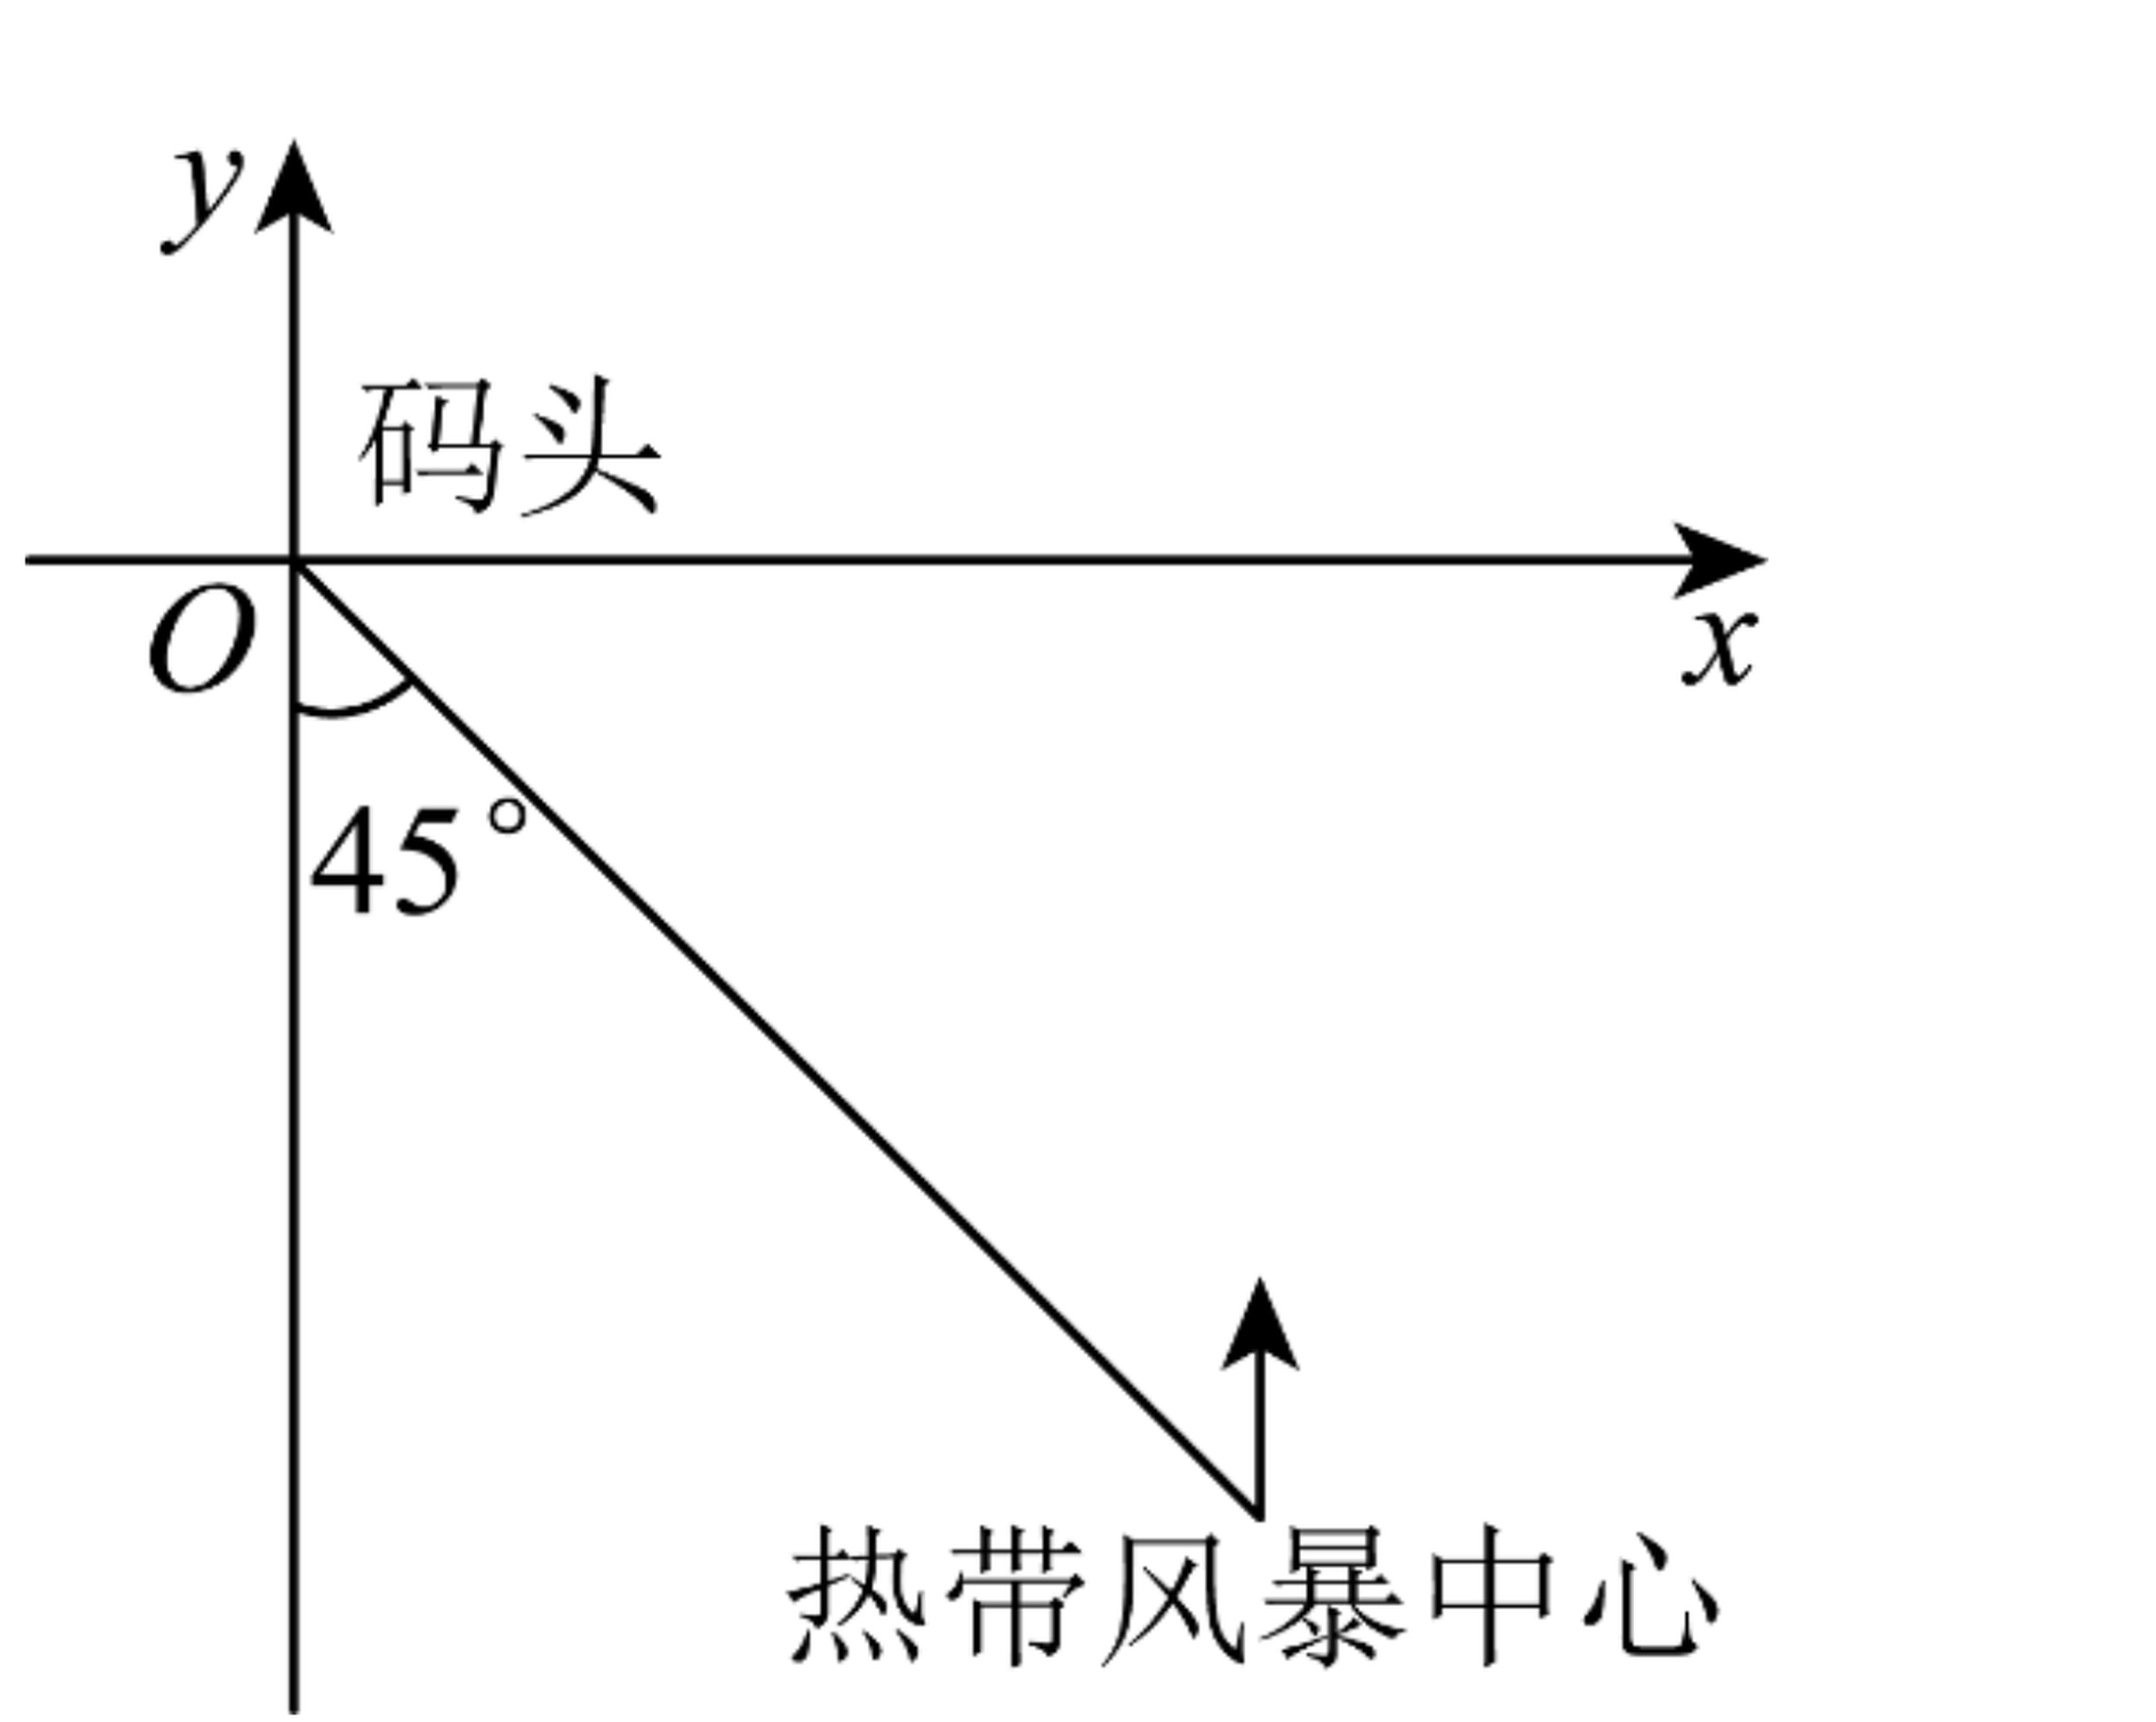
\includegraphics[width=0.36\textwidth]{figures/gao123_q5.png}
\end{center}

\ifanswer
\solbegin
\step{设风暴中心的坐标为 $(a,b)$，}
\step{由题意得 $a=400\sqrt2\times\cos45^\circ=400$，当 $a^2+b^2=400^2+b^2<500^2$，}% 原卷 $a^2$ 与 $400^2$ 并用，照录
\step{即 $-300<b<300$ 时，码头将受到风暴影响，}
\step{$\dfrac{300-(-300)}{20}=30h$，则码头受到风暴影响的时长为 30 小时，}
\step{所以由预报估计，该码头将受到热带风暴的影响时长大约为 30 小时.}
\solend
\fi

\item 已知 $a$、$b$、$c$ 为常数，若不等式 $\dfrac{ax-b}{x-c}\geqslant0$ 的解集为 $[-1,1)$，则不等式 $ax+b<0$ 的解集为\blankline[4.4em].

\ifanswer
\solbegin
\step{不等式 $\dfrac{ax-b}{x-c}\geqslant0$ 可化为 $(ax-b)(x-c)\geqslant0$ 且 $x-c\neq0$，}
\step{即 $a\left(x-\dfrac ba\right)(x-c)\geqslant0$ 且 $x\neq c$，}
\step{因为不等式 $\dfrac{ax-b}{x-c}\geqslant0$ 的解集为 $[-1,1)$，所以 $a<0$，且 $\dfrac ba=-1$,$c=1$，}
\step{即 $b=-a$，所以不等式 $ax+b<0$ 可化为 $ax-a<0$，又因为 $a<0$，所以 $x-1>0$，}
\step{解得 $x>1$，所以不等式 $ax+b<0$ 的解集为 $(1,+\infty)$.}
\solend
\fi

\item 已知实数 $a$、$b$ 满足 $ab=32$，且 $\log_2a=\log_b16$，则 $a+b$ 的值为\blankline[4.4em].

\ifanswer
\solbegin
\step{由 $\log_2a=\log_b16$，得 $\log_2a=\dfrac{\log_216}{\log_2b}$，则 $\log_2a\cdot\log_2b=4$，}
\step{由 $ab=32$，得 $\log_2a+\log_2b=\log_2ab=5$，}
\step{得 $\log_2a=1$,$\log_2b=4$ 或 $\log_2a=4$,$\log_2b=1$，}
\step{因此 $a=2$,$b=16$ 或 $a=16$,$b=2$，所以 $a+b=18$.}
\solend
\fi

\item 已知实数 $a$、$b$ 满足 $-3<a+2b<2$，$-1<2a-b<4$，则 $a+b$ 的取值范围为\blankline[4.4em].

\ifanswer
\solbegin
\step{设 $a+b=m(a+2b)+n(2a-b)=(m+2n)a+(2m-n)b$，}
\step{所以 $\begin{cases}m+2n=1\\2m-n=1\end{cases}$，解得 $n=\dfrac15$,$m=\dfrac35$，所以 $a+b=\dfrac35(a+2b)+\dfrac15(2a-b)$，}
\step{因为 $-3<(a+2b)<2$，$-1<2a-b<4$，}
\step{所以 $-\dfrac95<\dfrac35(a+2b)<\dfrac65$，$-\dfrac15<\dfrac15(2a-b)<\dfrac45$，}
\step{相加得 $-2<\dfrac35(a+2b)+\dfrac15(2a-b)<2$，即 $-2<a+b<2$，}
\step{故 $a+b$ 的取值范围为 $(-2,2)$.}
\solend
\fi

\item 存在 $x\in\R$ 使不等式 $\lvert2x-a\rvert<\lvert2a-1\rvert-2\lvert x\rvert$ 成立，则实数 $a$ 的取值范围是\blankline[4.4em].

\ifanswer
\solbegin
\step{存在 $x\in\R$，不等式 $\lvert2x-a\rvert<\lvert2a-1\rvert-2\lvert x\rvert$ 成立，}
\step{变形即 $\lvert2x-a\rvert+2\lvert x\rvert<\lvert2a-1\rvert$ 成立，}
\step{由于 $\lvert2x-a\rvert+\lvert2x\rvert\geqslant\lvert(2x-a)-2x\rvert=\lvert a\rvert$，当且仅当 $2x(2x-a)\leqslant0$ 时取等号，}
\step{因此有 $\lvert a\rvert<\lvert2a-1\rvert$，两边平方 $a^2<(2a-1)^2$，解得 $a>1$ 得 $a<\dfrac13$，}% 原卷“解得 a>1 得 a<1/3”，照录
\step{即实数 $a$ 的取值范围是 $\left(-\infty,\dfrac13\right)\cup(1,+\infty)$.}
\solend
\fi

\item 已知集合 $A=\{(x,y)\mid x^2+mx-y+2=0\}$，$B=\{(x,y)\mid x-y+1=0,0\leqslant x\leqslant3\}$，若集合 $A\cap B$ 的子集个数为 $2$，则实数 $m$ 的取值范围为\blankline[4.4em].

\ifanswer
\solbegin
\step{因为集合 $A\cap B$ 的子集个数为 $2$，所以 $A\cap B$ 的元素有一个，}
\step{即 $\begin{cases}x^2+mx-y+2=0\\x-y+1=0\end{cases}$ 在 $x\in[0,3]$ 上只有一个解，}
\step{即 $x^2+(m-1)x+1=0$ 在 $[0,3]$ 上只有一个解，}
\step{即 $1-m=x+\dfrac1x$ 在 $[0,3]$ 上只有一个解，}
\step{结合对勾函数的性质得 $1-m=2$ 或 $1-m>\dfrac{10}{3}$，解得 $m=-1$ 或 $m<-\dfrac73$.}
\solend
\fi

\item $[x]$ 表示不超过 $x$ 的最大整数，则集合 $A=\left\{y\,\middle\vert\,y=\left[\dfrac{x^2}{100}\right],x=1,2,3,\cdots,100\right\}$ 中的元素个数为\blankline[4.4em].

\ifanswer
\solbegin
\step{记 $a_k=\left[\dfrac{k^2}{100}\right](k=1,2,\cdots,100)$，$a_k$ 随 $k$ 增大而单调不减.}
\step{当 $k\geqslant50$ 时，$\dfrac{(k+1)^2}{100}-\dfrac{k^2}{100}=\dfrac{2k+1}{100}\geqslant\dfrac{101}{100}>1$，所以 $a_{k+1}\geqslant a_k+1$，}
\step{即 $a_{50}$、$a_{51}$、$\cdots$、$a_{100}$ 两两互异.}
\step{又 $a_{50}=\left[\dfrac{2500}{100}\right]=25$、$a_{100}=100$，这一段共 $100-50+1=51$ 个互异的值，}
\step{且都大于等于 $25$.}
\step{当 $k\leqslant49$ 时，$\dfrac{(k+1)^2}{100}-\dfrac{k^2}{100}=\dfrac{2k+1}{100}\leqslant\dfrac{99}{100}<1$，即 $a_k$ 每次至多增加 $1$；}
\step{又 $a_1=0$、$a_{49}=\left[\dfrac{2401}{100}\right]=24$，}
\step{故 $a_1$、$a_2$、$\cdots$、$a_{49}$ 依次取遍 $0$，$1$，$2$，$\cdots$，$24$，共 $25$ 个值.}
\step{两段取值范围互不重叠（前段不超过 $24$、后段不小于 $25$），}
\step{所以集合 $A$ 中共有 $25+51=76$ 个元素.}
\solend
\fi

\item 若实数 $a$、$b$、$c$ 满足 $\dfrac1{2^a}+\dfrac1{2^b}=1$，$\dfrac1{2^{a+b}}+\dfrac1{2^{b+c}}+\dfrac1{2^{a+c}}=1$，则 $c$ 的最大值是\blankline[4.4em].

\ifanswer
\solbegin
\step{因为 $\dfrac1{2^a}+\dfrac1{2^b}=1$，}
\step{由基本不等式得 $1=\dfrac1{2^a}+\dfrac1{2^b}\geqslant2\sqrt{\dfrac1{2^a}\cdot\dfrac1{2^b}}$（当且仅当 $a=b=1$ 时取等号），}
\step{所以 $\dfrac1{2^a}\cdot\dfrac1{2^b}\leqslant\dfrac14$，所以 $-\dfrac1{2^a}\cdot\dfrac1{2^b}\geqslant-\dfrac14$，}% 原卷带负号起论，照录
\step{因为 $\dfrac1{2^{a+b}}+\dfrac1{2^{b+c}}+\dfrac1{2^{a+c}}=1$，$\dfrac1{2^{b+c}}+\dfrac1{2^{a+c}}=\dfrac1{2^c}\left(\dfrac1{2^a}+\dfrac1{2^b}\right)=\dfrac1{2^c}$，}
\step{所以 $\dfrac1{2^c}=1-\dfrac1{2^{a+b}}\geqslant\dfrac34$，所以 $2^c\leqslant\dfrac43$，所以 $c\leqslant\log_2\dfrac43=2-\log_23$，}
\step{故 $c$ 的最大值是 $2-\log_23$.}
\solend
\fi

\end{enumerate}

\bigsec{二、选择题}

\begin{enumerate}
\setcounter{enumi}{12}

\item 下列运用等式或不等式的性质变形中，正确的是\mbox{（\quad）}

\keepwithprev
A. 如果 $a=b$，那么 $\dfrac ac=\dfrac bc$\qquad\qquad B. 如果 $\dfrac1a<\dfrac1b<0$，那么 $a-\dfrac1a>b-\dfrac1b$

C. 如果 $a>b$，那么 $\dfrac1a<\dfrac1b$\qquad\qquad D. 如果 $a>b>0$，$m\in\R$，那么 $\dfrac ba<\dfrac{b+m}{a+m}$

\ifanswer
\solbegin
\step{对于 $A$，若 $c=0$，$A$ 错误；}
\step{对于 $B$，若 $\dfrac1a<\dfrac1b<0$，则 $0>a>b$，$-\dfrac1a>-\dfrac1b>0$，}
\step{所以 $a-\dfrac1a>b-\dfrac1b$，$B$ 正确；}
\step{对于 $C$，$a>0$，$b<0$ 时，$C$ 错误；}
\step{对于 $D$，$\dfrac{b+m}{a+m}-\dfrac ba=\dfrac{ab+am}{a(a+m)}-\dfrac{ab+bm}{a(a+m)}=\dfrac{(a-b)m}{a(a+m)}$，}
\step{因为 $a>b>0$，所以 $a-b>0$，但 $m$、$a+m$ 的符号不确定，}
\step{当 $m=0$ 时，$\dfrac ba=\dfrac{b+m}{a+m}$，}
\step{当 $m(a+m)>0$ 时，$\dfrac ba<\dfrac{b+m}{a+m}$，当 $m(a+m)<0$ 时，$\dfrac ba>\dfrac{b+m}{a+m}$，$D$ 错误.}
\step{故选 $B$.}
\solend
\fi

\item “$a>b$”的一个必要非充分条件是\mbox{（\quad）}

\keepwithprev
A. $ac^2>bc^2$\qquad\quad B. $2^a>2^b$\qquad\quad C. $\left(\dfrac12\right)^{a-b}\leqslant1$\qquad\quad D. $a^3>b^3$

\ifanswer
\solbegin
\step{即“$a>b$”能推出选项，但选项不能推出“$a>b$”，故选 $C$.}
\solend
\fi

\item 若 $A=\left\{x\,\middle\vert\,x=\dfrac k6+1,k\in\Z\right\}$，$B=\left\{x\,\middle\vert\,x=\dfrac k3+\dfrac12,k\in\Z\right\}$，$C=\left\{x\,\middle\vert\,x=\dfrac{2k}{3}+\dfrac12,k\in\Z\right\}$，则这三个集合间的关系是\mbox{（\quad）}

\keepwithprev
A. $A\subseteq B\subseteq C$\qquad\quad B. $A\subseteq C\subseteq B$\qquad\quad C. $C\subseteq B\subseteq A$\qquad\quad D. $C\subseteq A\subseteq B$

\ifanswer
\solbegin
\step{若 $x\in C$，则存在 $k_0\in\Z$，使 $x=\dfrac{2k_0}{3}+\dfrac12$，}
\step{又 $2k_0\in\Z$，所以 $x\in B$，故 $C\subseteq B$，}
\step{若 $x\in B$，则存在 $k_1\in\Z$，使 $x=\dfrac{k_1}{3}+\dfrac12=\dfrac{2k_1-3}{6}+1$，}
\step{又 $2k_1-3\in\Z$，所以 $x\in A$，故 $B\subseteq A$，}
\step{又 $\dfrac43\in A$，$\dfrac43\notin B$，$\dfrac56\in B$，$\dfrac56\notin C$，所以 $C\subseteq B\subseteq A$，故选 $C$.}
\solend
\fi

\item 集合 $S=\{x\mid(x+a)(x^2+bx+c)=0\}$，$T=\{x\mid(ax+1)(cx^2+bx+1)=0\}$，其中 $a$、$b$、$c$ 为实数，若 $\lvert S\rvert$、$\lvert T\rvert$ 分别表示 $S$、$T$ 的元素个数，则下列结论中一定成立的是\mbox{（\quad）}

\keepwithprev
A. 若 $\lvert T\rvert=0$，则 $\lvert S\rvert=1$\qquad\qquad B. 若 $\lvert S\rvert=1$，则 $\lvert T\rvert=1$

C. 若 $\lvert S\rvert=2$，则 $\lvert T\rvert=2$\qquad\qquad D. 若 $\lvert T\rvert=3$，则 $\lvert S\rvert=2$

\ifanswer
\solbegin
\step{令 $f(x)=(x+a)(x^2+bx+c)$,$g(x)=(ax+1)(cx^2+bx+1)$，}
\step{对于选项 A，当 $\lvert T\rvert=0$ 时，方程 $g(x)=(ax+1)(cx^2+bx+1)=0$ 无实根，}
\step{当 $a=b=c=0$ 时，$f(x)=x^3$，由 $f(x)=0$ 得 $x=0$，此时 $\lvert S\rvert=1$；}
\step{当 $a=0$,$b^2-4c<0$ 时，$f(x)=x(x^2+bx+c)$，由 $f(x)=0$ 得 $x=0$，}
\step{此时 $\lvert S\rvert=1$，所以选项 A 正确；}
\step{对于选项 B，若 $\lvert S\rvert=1$，则 $f(x)=(x+a)(x^2+bx+c)=0$ 有且只有一根，}
\step{又 $x=-a$ 一定是 $f(x)=0$ 的根，所以 $\triangle=b^2-4c<0$，}
\step{又 $\triangle=b^2-4c<0$ 且 $a=0$ 时，$g(x)=(ax+1)(cx^2+bx+1)=0$ 无解，}
\step{此时 $\lvert T\rvert=0$，所以选项 B 错误，}
\step{对于选项 C，若 $\lvert S\rvert=2$ 时，则 $f(x)=(x+a)(x^2+bx+c)=0$ 有且只有 $2$ 根，}
\step{又 $x=-a$ 一定是 $f(x)=0$ 的根，}
\step{所以 $\triangle=b^2-4c=0$ 且 $a^2+ab+c\neq0$ 或 $\triangle=b^2-4c>0$ 且 $a^2+ab+c=0$，}
\step{当 $a=0$ 时，存在 $b$,$c$，使 $\triangle=b^2-4c=0$ 且 $a^2+ab+c\neq0$，}
\step{此时 $g(x)=(ax+1)(cx^2+bx+1)=0$ 只有一根，所以选项 C 错误，}
\step{对于选项 D，当 $\lvert T\rvert=3$ 时，方程 $g(x)=(ax+1)(cx^2+bx+1)=0$ 有三个根，}
\step{所以 $a\neq0$,$c\neq0$,$b^2-4c>0$，}
\step{设 $x_0$ 为 $g(x)=0$ 的一个根，即 $(ax_0+1)(cx_0^2+bx_0+1)=0$，}
\step{则 $x_0\neq0$，且 $f\left(\dfrac1{x_0}\right)=\left(\dfrac1{x_0}+a\right)\left(\dfrac1{x_0^2}+\dfrac1{x_0}b+c\right)=\dfrac1{x_0^3}g(x_0)=0$，}
\step{所以 $\dfrac1{x_0}$ 为方程 $f(x)=0$ 的根，故 $f(x)=0$ 有三个根，即 $\lvert T\rvert=3$ 时，}
\step{必有 $\lvert S\rvert=3$，所以选项 D 错误，}
\step{故选 $A$.}
\solend
\fi

\end{enumerate}

% 第 17 题是解答题第一题且带文氏图，守卫放在 \bigsec 之前，连节标题一起量页高
\needvspace{7cm}
\bigsec{三、解答题}

\begin{enumerate}
\setcounter{enumi}{16}

\item 设全集 $U=\R$，集合 $A=\{x\mid-2\leqslant x\leqslant4\}$，$B=\{x\mid x<-6$ 或 $x\geqslant2\}$.

（1）求图中阴影部分表示的集合；

（2）已知集合 $C=\{x\mid10-a<x<2a+1\}$，若 $\overline B\cap C=\varnothing$，求 $a$ 的取值范围.

\begin{center}
% 图取原卷截图（第 7 页题干右侧）、去水印后 2× LANCZOS 放大，本稿移至题干之后
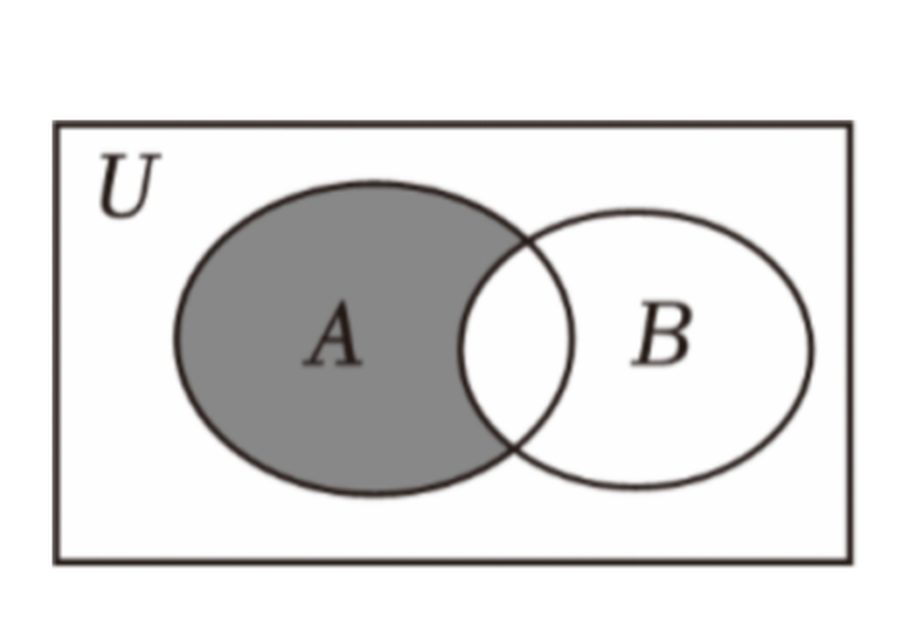
\includegraphics[width=0.34\textwidth]{figures/gao123_q17.png}
\end{center}

\ifanswer
\solbegin
\step{（1）$A\cap B=\{x\mid2\leqslant x\leqslant4\}$，}
\step{则图中阴影部分表示 $\overline{A\cap B}=\{x\mid-2\leqslant x<2\}$.}% 原卷把上划线盖在整个 $A\cap B$ 上，照录
\step{（2）由题意得 $\overline B=\{x\mid-6\leqslant x<2\}$，$C\subseteq B$，}
\step{所以当 $C=\varnothing$ 时，$10-a\geqslant2a+1$，解得 $a\leqslant3$，符合题意；}
\step{当 $C\neq\varnothing$ 时，$\begin{cases}10-a<2a+1\\2a+1\leqslant-6\end{cases}$ 或者 $\begin{cases}10-a<2a+1\\10-a\geqslant2\end{cases}$，}
\step{此时不等式组 $\begin{cases}10-a<2a+1\\2a+1\leqslant-6\end{cases}$ 无解，}
\step{不等式组 $\begin{cases}10-a<2a+1\\10-a\geqslant2\end{cases}$ 的解集为 $3<a\leqslant8$，}
\step{综上，$a$ 的取值范围为 $\{a\mid a\leqslant8\}$.}
\solend
\fi

\item (1) 求不等式：$\lvert x-1\rvert+\lvert x-2\rvert\leqslant5$ 的解集.

(2) 当 $m<1$ 时，解关于 $x$ 的不等式 $\dfrac{m(x-3)}{x+2}>1$.

\ifanswer
\solbegin
\step{(1) 当 $x<1$ 时，$\lvert x-1\rvert+\lvert x-2\rvert\leqslant5\Leftrightarrow-x+1+2-x\leqslant5$，}
\step{解得 $-1\leqslant x<1$；}
\step{当 $1\leqslant x\leqslant2$ 时，$\lvert x-1\rvert+\lvert x-2\rvert\leqslant5\Leftrightarrow x-1+2-x=1\leqslant5$ 恒成立，}
\step{所以 $1\leqslant x\leqslant2$；}
\step{当 $x>2$ 时，$\lvert x-1\rvert+\lvert x-2\rvert\leqslant5\Leftrightarrow x-1+x-2=2x-3\leqslant5$，}
\step{解得 $2<x\leqslant4$.}
\step{综上所述，不等式 $\lvert x-1\rvert+\lvert x-2\rvert\leqslant5$ 的解集为 $[-1,4]$.}
\step{(2) 原不等式变成 $\dfrac{(m-1)x-(3m+2)}{x+2}>0$，$n<1$，所以 $n-1<0$，}% 原卷作 $n<1$、$n-1<0$，与题设 $m<1$ 字母不一致，照录
\step{所以原不等式变成 $\dfrac{x-\dfrac{3m+2}{m-1}}{x+2}<0$，$\dfrac{3m+2}{m-1}-(-2)=\dfrac{5m}{m-1}$，}
\step{所以 $m<0$ 时，$\dfrac{5m}{m-1}>0$，$\dfrac{3m+2}{m-1}>-2$，}
\step{原不等式的解集为 $\left(-2,\dfrac{3m+2}{m-1}\right)$；}
\step{$m=0$ 时，原不等式变成 $1<0$，无解；}
\step{$0<m<1$ 时，$\dfrac{5m}{m-1}<0$，$\dfrac{3m+2}{m-1}<-2$，}
\step{原不等式的解集为 $\left(\dfrac{3m+2}{m-1},-2\right)$.}
\solend
\fi

\item 在园林博览会上，某公司带来了一种智能设备供采购商洽谈采购，并决定大量投放市场，已知该种设备年固定研发成本为 $50$ 万元，每生产一台需另投入 $100$ 元，设该公司一年内生产该设备 $x$ 万台且全部售完，每万台的销售收入 $G(x)$（万元）与年产量 $x$（万台）满足如下关系式：$G(x)=\begin{cases}180-x,0<x\leqslant20\\80+\dfrac{2000}{x}-\dfrac{8000}{x(x-1)},x>20\end{cases}$.

(1) 写出年利润 $W(x)$（万元）关于年产量 $x$（万台）的函数解析式；（利润 $=$ 销售收入 $-$ 成本）

(2) 当年产量为多少万台时，该公司获得的年利润最大，并求出最大利润.

\ifanswer
\solbegin
\step{(1) $W(x)=xG(x)-50-100x=\begin{cases}-50+80x-x^2,0<x\leqslant20\\-20x+1950-\dfrac{8000}{x-1},x>20\end{cases}$；}
\step{(2) 当 $0<x\leqslant20$ 时，$W(x)=-50+80x-x^2=-(x-40)^2+1550$，}
\step{由函数性质得当 $x\leqslant40$ 时严格增，所以当 $x=20$ 时，$W(x)_{max}=1150$，}
\step{当 $x>20$ 时，$W(x)=-20x+1950-\dfrac{8000}{x-1}=-20\left[(x-1)+\dfrac{400}{x-1}\right]+1930$，}
\step{$W(x)=-20\left[(x-1)+\dfrac{400}{x-1}\right]+1930\leqslant-20\times2\sqrt{(x-1)\cdot\dfrac{400}{x-1}}+1930$}
\step{$=1130$，当且仅当 $x-1=\dfrac{400}{x-1}$，即 $x=21$ 时取等号，}
\step{所以 $W(x)_{max}=1130$，}
\step{因为 $1150>1130$，所以当 $x=20$ 时，$W(x)_{max}=1150$，}
\step{即当年产量为 $20$ 万台时，该公司获得的年利润最大，}
\step{最大利润为 $1150$ 万元.}
\solend
\fi

\item 关于 $x$ 的方程 $(x^2-1)^2-2k\lvert x^2-1\rvert+k+1=0(k\in\R)$.

(1) 若方程无实根，求 $k$ 的取值范围；

(2) 若方程有 $4$ 个不等实根，求 $k$ 的取值范围；

(3) 若 $k=a+b$，且满足 $\dfrac1{a+2b}+\dfrac1{a+3}=\dfrac12$，$a>0$，$b>0$，试判断方程根的个数.

\ifanswer
\solbegin
\step{(1) 关于 $x$ 的方程 $(x^2-1)^2-2k\lvert x^2-1\rvert+k+1=0(k\in\R)$，}
\step{令 $t=\lvert x^2-1\rvert$，则 $t\geqslant0$，则原方程转化为 $t^2-2kt+k+1=0(*)$，}
\step{因为关于 $x$ 的方程 $(x^2-1)^2-2k\lvert x^2-1\rvert+k+1=0(k\in\R)$ 无实根，}
\step{所以 $(*)$ 式无实根或实根均小于零，令 $f(t)=t^2-2kt+k+1$，}
\step{①若 $(*)$ 式无实根，则 $\triangle<0$，解得 $\dfrac{1-\sqrt5}{2}<k<\dfrac{1+\sqrt5}{2}$，}
\step{②两根均为负，则 $\begin{cases}\Delta\geqslant0\\t_{\text{对}}=k<0\\f(0)>0\end{cases}$，解得 $-1<k\leqslant\dfrac{1-\sqrt5}{2}$，}
\step{综合①②，得 $k$ 的取值范围是 $\left(-1,\dfrac{1+\sqrt5}{2}\right)$；}
\step{(2) 作函数 $t=\lvert x^2-1\rvert$ 的图象，}
\begin{center}
% 图取原卷截图（第 11 页解析内）、去水印后 2× LANCZOS 放大，仅答案版出
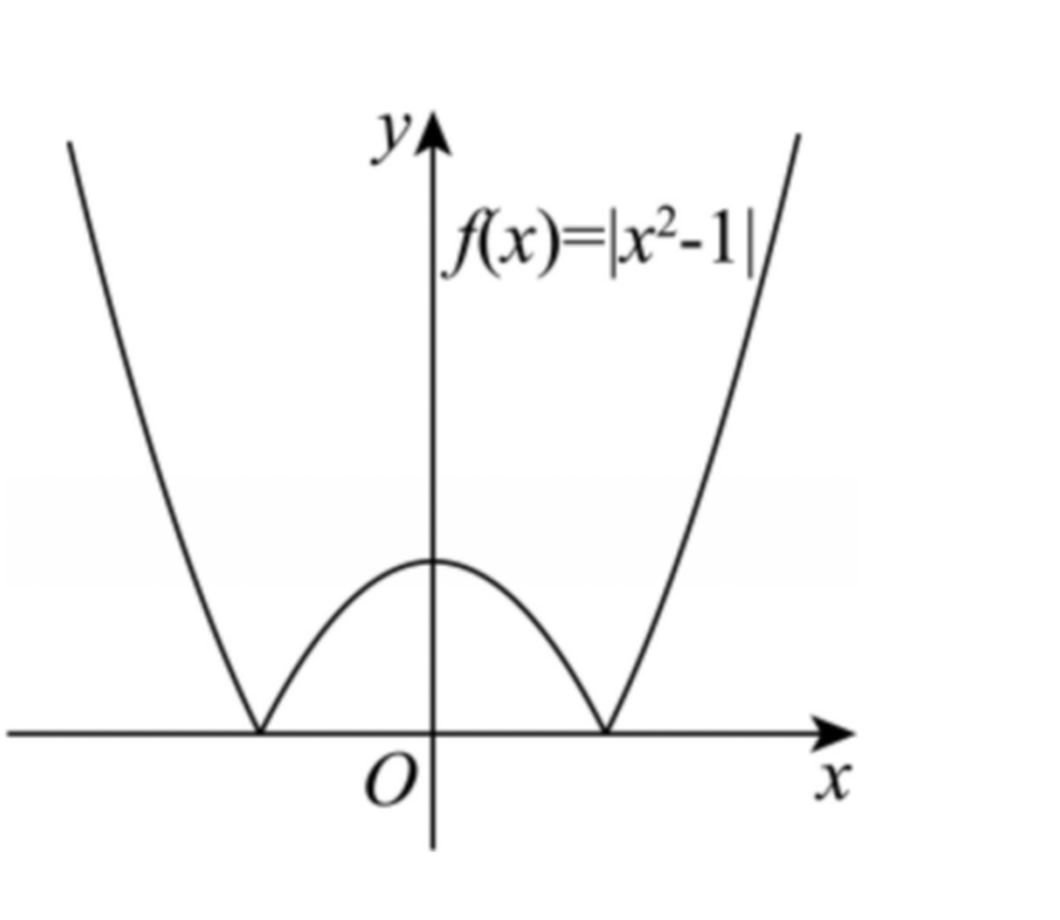
\includegraphics[width=0.40\textwidth]{figures/gao123_q20.png}
\end{center}
\step{$t=0$ 或 $t>1$ 时，每一个 $t$ 值对应 $2$ 个不同的 $x$ 值，}
\step{$t=1$ 时一个 $t$ 值对应 $3$ 个不同的 $x$ 值，}
\step{$0<t<1$ 时一个 $t$ 值对应 $4$ 个不同的 $x$ 值，}
\step{要使原方程有四个不等实根，}
\step{①$(*)$ 式一根为零，另一根大于 $1$，无解；}
\step{②$(*)$ 有两不等根且两根均大于 $1$，则 $\begin{cases}\Delta>0\\t_{\text{对}}=k>1\\f(1)>0\end{cases}$，解得 $\dfrac{1+\sqrt5}{2}<k<2$；}
\step{④$(*)$ 式有 $1$ 实根在 $(0,1)$ 之间，另一根小于零，}% 原卷由 ② 直接跳到 ④，缺 ③，照录
\step{则 $\begin{cases}f(0)<0\\f(1)>0\end{cases}$，所以 $\begin{cases}k+1<0\\2-k>0\end{cases}$，解得 $k<-1$，}
\step{综上所述，$k$ 取值范围为 $(-\infty,-1)\cup\left(\dfrac{1+\sqrt5}{2},2\right)$；}
\step{(3) 因为 $\dfrac1{a+2b}+\dfrac1{a+3}=\dfrac{a+2b+a+3}{(a+2b)(a+3)}=\dfrac{2(a+b)+3}{(a+2b)(a+3)}=\dfrac12$，}
\step{所以 $2(a+b)+3=\dfrac12(a+2b)(a+3)$，}
\step{因为 $a$、$b$ 为正实数，所以 $\dfrac12=\dfrac1{a+2b}+\dfrac1{a+3}\geqslant2\sqrt{\dfrac1{a+2b}\times\dfrac1{a+3}}$，}
\step{得 $\dfrac1{16}\geqslant\dfrac1{a+2b}\times\dfrac1{a+3}$，即 $(a+2b)(a+3)\geqslant16$，}
\step{所以 $2(a+b)+3\geqslant8$，即 $a+b\geqslant\dfrac52$，}
\step{当且仅当 $\dfrac1{a+2b}=\dfrac1{a+3}$ 即 $a=1$,$b=\dfrac32$ 时取等号，}
\step{故 $k\geqslant\dfrac52$，此时有 $\begin{cases}\Delta>0\\t_{\text{对}}=k>1\\f(0)>0,f(1)<0\end{cases}$，}
\step{故 $(*)$ 式有两不等实根且一根在 $(0,1)$ 之间，另一根大于 $1$，}
\step{故原方程有 $6$ 个实根.}
\solend
\fi

\item 设 $n$ 是不小于 $3$ 的正整数，集合 $S_n=\{(a_1,a_2,\cdots,a_n)\mid a_i\in\{0,1\},i=1,2,\cdots,n\}$，对于集合 $S_n$ 中任意两个元素 $A=(a_1,a_2,\cdots,a_n)$，$B=(b_1,b_2,\cdots,b_n)$.

定义 1：$A\cdot B=n-(\lvert a_1-b_1\rvert+\lvert a_2-b_2\rvert+\cdots+\lvert a_n-b_n\rvert)$，

定义 2：若 $A\cdot B=0$，则称互为相反元素，记作 $A=\overline B$ 或 $B=\overline A$.

(1) 若 $n=3$，$A=(0,1,0)$，$B=(1,1,0)$，试写出 $\overline A$、$\overline B$ 以及 $A\cdot B$ 的值；

(2) 若 $A$、$B\in S_n$，$A=(a_1,a_2,\cdots,a_n)$，$B=(b_1,b_2,\cdots,b_n)$，证明：$A\cdot B+\overline A\cdot B=n$；

(3) 设 $k$ 是小于 $n$ 的正奇数，至少含有两个元素的集合 $M\subseteq S_n$，且对于集合 $M$ 中任意两个不相同的元素 $A=(a_1,a_2,\cdots,a_n)$，$B=(b_1,b_2,\cdots,b_n)$，都有 $A\cdot B=n-k$，试求集合 $M$ 中元素个数的所有可能值.

\ifanswer
\solbegin
\step{(1) $\overline A=(1,0,1)$,$\overline B=(0,0,1)$,$\overline A\cdot\overline B=2$；}
\step{(2) 设 $A=(a_1,a_2,\cdots,a_n)$,$B=(b_1,b_2,\cdots,b_n)$,$\overline A=(x_1,x_2,\cdots,x_n)$，}
\step{由 $a_i$、$b_i$、$x_i\in\{0,1\}$，$i=1,2,\cdots,n$，得 $\lvert a_i-x_i\rvert\leqslant1$，$i=1,2,\cdots,n$，}
\step{所以 $\lvert a_1-x_1\rvert+\lvert a_2-x_2\rvert+\cdots+\lvert a_i-x_i\rvert\leqslant n$，}% 原卷末项下标作 $i$，照录
\step{当且仅当 $\lvert a_i-x_i\rvert=1$，$i=1,2,\cdots,n$，}
\step{即 $x_i=1-a_i$，$i=1,2,\cdots,n$ 时取等号.}
\step{由题意得 $A\cdot\overline A=n-(\lvert a_1-x_1\rvert+\lvert a_2-x_2\rvert+\cdots+\lvert a_n-x_n\rvert)=0$，}
\step{即 $\lvert a_1-x_1\rvert+\lvert a_2-x_2\rvert+\cdots+\lvert a_n-x_n\rvert=n$，}
\step{所以 $x_i=1-a_i$，$i=1,2,\cdots,n$，}
\step{$A\cdot B+\overline A\cdot B=2n-\sum\limits_{i=1}^n[\lvert a_i-b_i\rvert+(1-a_i)-b_i]$}
\step{$=2n-\sum\limits_{i=1}^n(\lvert1-b_i\rvert+\lvert0-b_i\rvert)=2n-\sum\limits_{i=1}^n(1-b_i+b_i)=2n-n=n$；}
\step{(3) 假设 $A=(a_1,a_2,\cdots,a_n)$，$B=(b_1,b_2,\cdots,b_n)$，$C=(c_1,c_2,\cdots,c_n)$}
\step{为集合 $M$ 中的三个不相同的元素，}
\step{则 $A\cdot B=n-(\lvert a_1-b_1\rvert+\lvert a_2-b_2\rvert+\cdots+\lvert a_n-b_n\rvert)=n-k$，}
\step{即 $\lvert a_1-b_1\rvert+\lvert a_2-b_2\rvert+\cdots+\lvert a_n-b_n\rvert=k$，}
\step{又由题意得 $\lvert a_i-b_i\rvert=0$ 或 $1$，$i=1,2,\cdots,n$，}
\step{$\lvert a_1-b_1\rvert$、$\lvert a_2-b_2\rvert$、$\cdots$、$\lvert a_n-b_n\rvert$ 恰有 $k$ 个 $1$，$n-k$ 个 $0$，}
\step{设其中 $k$ 个等于 $1$ 的项以此为 $a_{m_1}-b_{m_1}$,$a_{m_2}-b_{m_2}$,$\cdots$,$a_{m_k}-b_{m_k}$，}
\step{$n-k$ 个等于 $0$ 的项为 $a_{m_{k+1}}-b_{m_{k+1}}$,$a_{m_{k+2}}-b_{m_{k+2}}$,$\cdots$,$a_{m_n}-b_{m_n}$，}
\step{由题意得 $A\cdot C=n-(\lvert a_1-c_1\rvert+\lvert a_2-c_2\rvert+\cdots+\lvert a_n-c_n\rvert)=n-k$，}
\step{所以 $\sum\limits_{i=1}^k\lvert a_{m_i}-c_{m_i}\rvert+\sum\limits_{j=k+1}^n\lvert a_{m_j}-c_{m_j}\rvert=k$ ①，}
\step{同理 $\sum\limits_{i=1}^k\lvert b_{m_i}-c_{m_i}\rvert+\sum\limits_{j=k+1}^n\lvert b_{m_j}-c_{m_j}\rvert=k$ ②，}
\step{因为 $\lvert a_{m_{k+1}}-b_{m_{k+1}}\rvert=\lvert a_{m_{k+2}}-b_{m_{k+2}}\rvert=\cdots=\lvert a_{m_n}-b_{m_n}\rvert=0$，}
\step{所以 $\sum\limits_{j=k+1}^n\lvert a_{m_j}-c_{m_j}\rvert=\sum\limits_{j=k+1}^n\lvert b_{m_j}-c_{m_j}\rvert$，}
\step{由①$-$②得 $\sum\limits_{i=1}^k(\lvert a_{m_i}-c_{m_i}\rvert-\lvert b_{m_i}-c_{m_i}\rvert)=0$，}
\step{又 $\sum\limits_{i=1}^k(\lvert a_{m_i}-c_{m_i}\rvert-\lvert b_{m_i}-c_{m_i}\rvert)=\sum\limits_{i=1}^k(\lvert1-c_{m_i}\rvert-\lvert0-c_{m_i}\rvert)=k-2\sum\limits_{i=1}^k c_{m_i}$}
\step{为奇数，与 $\sum\limits_{i=1}^k(\lvert a_{m_i}-c_{m_i}\rvert-\lvert b_{m_i}-c_{m_i}\rvert)=0$ 矛盾，所以假设不成立，}
\step{即集合 $M$ 中至多有两个元素，}
\step{当 $M=\{(1,1,\cdots,1,0,0,\cdots,0),(0,0,\cdots,0)\}$ 时符合题意，}
\step{所以集合 $M$ 中元素的个数只可能是 $2$.}
\solend
\fi

\end{enumerate}

\end{document}
"
% 紧凑版：xelatex "\def\iscompact{1}% 高一123_行知中学_10月月考.tex
%   —— 高一上数学“2026-2027 年行知中学高一上 10 月月考”（试卷版/答案版）
% 试卷版：xelatex 高一123_行知中学_10月月考.tex
% 答案版：xelatex "\def\isanswer{1}% 高一123_行知中学_10月月考.tex
%   —— 高一上数学“2026-2027 年行知中学高一上 10 月月考”（试卷版/答案版）
% 试卷版：xelatex 高一123_行知中学_10月月考.tex
% 答案版：xelatex "\def\isanswer{1}% 高一123_行知中学_10月月考.tex
%   —— 高一上数学“2026-2027 年行知中学高一上 10 月月考”（试卷版/答案版）
% 试卷版：xelatex 高一123_行知中学_10月月考.tex
% 答案版：xelatex "\def\isanswer{1}\input{高一123_行知中学_10月月考.tex}"
% 紧凑版：xelatex "\def\iscompact{1}\input{高一123_行知中学_10月月考.tex}"
%
% 原始材料：微信公众号“魔都数学加油站”文章，作者破晓，2026-11-09 17:52 发布；
% 连载“27学年高一123”，原文标题“27学年高一123——2026-2027年上海市行知中学高一上10月月考”；
% 原文链接：https://mp.weixin.qq.com/s/GV4SWBLUJrBhMQwo22FVzg。
% 正文为 14 张 PNG 页（第 7、9、11、13、14 页 2560×3620，其余 4762×6735），
% 题目下印有【答案】或【解析】，为讲评版。
% 题目、解析均据原图转录；卷面红色水印及公众号页脚未录入。
% 全卷 3 张插图：第 5 题的坐标示意图、第 17 题的文氏图（均属题干，三版都出）、
% 第 20 题 (2) 的 $t=\lvert x^2-1\rvert$ 图象（属解析，仅答案版出）；
% 都取原卷截图去水印、2× LANCZOS 放大，见 figures/gao123_q5.png、
% figures/gao123_q17.png、figures/gao123_q20.png。
%
% 卷首标题：原卷印作“2026-2027 年行知中学高一上 10 月月考”（公众号标题中的“上海市”
% 卷面标题行没有，本稿照卷面），年份区间按全稿惯例排 en dash；原卷未印副标题，本稿按题目内容
% 标为“集合与常用逻辑用语、不等式”（与 110／111／113／116／118／120 同）。
%
% 与原卷的排版差异：
%   ① 原文从第 3 题起，填空题编号为 3—12、选择题为 13—16、解答题为 17—21，本稿保留原题号；
%   ② 原卷每题下直接印【解析】／【答案】，本稿按全稿惯例置于答案版；第 3 题只印【答案】、
%      另提 \ans{}；选择题答案在解析末句“故选 …”，括号内留空；
%   ③ 原卷未印副标题，本稿按“知识模块”口径补出；
%   ④ 原卷填空横线按全稿惯例排为 \blankline[4.4em]；选择题括号排 \mbox{（\quad）}、
%      选项段前按惯例加 \keepwithprev；解答题不留作答区（原卷为讲评版，与 109—122 同）；
%   ⑤ 原卷数集排斜体 $R$／$Z$（第 9 题作粗体 $\mathbf{R}$），按全稿惯例改 \R／\Z；
%      绝对值按全稿惯例排 \lvert…\rvert，集合描述竖线排 \mid；单位 km、h 原卷排斜体，
%      本稿按正体照排；补集照原卷上划线排 \overline{B}、\overline{A}。
%
% 判别式与子集符号：第 16 题解析的 $\triangle=b^2-4c<0$、第 20 题 (1) ① 的 $\triangle<0$
%   均作等边、扁的 \triangle；第 20 题 ② 两处 cases 与 (3) 的 $\Delta\geqslant0$／$\Delta>0$
%   作等腰、高的 \Delta，逐处照录、不统一；第 15 题选项与第 17 题 (2) 的 $\subseteq$
%   印有下划线，照录 \subseteq。
%
% 原卷存疑照录：
%   第 4 题解析“若 $-\lvert a\rvert=0$，则 $a=0$，则 $A=\{0,-1,0\}$”以元素重复说明互异性；
%   第 5 题解析“当 $a^2+b^2=400^2+b^2<500^2$”等式左边 $a^2$ 与 $400^2$ 并用；
%   第 9 题解析“解得 $a>1$ 得 $a<\dfrac13$”（按平方不等式应为 $a>1$ 或 $a<\dfrac13$）；
%   第 12 题解析“所以 $-\dfrac1{2^a}\cdot\dfrac1{2^b}\geqslant-\dfrac14$”带负号起论；
%   第 17 题 (1) 解析把阴影部分（实为 $A\cap\overline B$）印作 $\overline{A\cap B}$；
%   第 18 题 (2) 解析作“$n<1$，所以 $n-1<0$”，与题设 $m<1$ 字母不一致；
%   第 20 题 (2) 的情形编号由 ①、② 直接跳到 ④（缺 ③）；
%   第 21 题 (2) 解析“$\lvert a_1-x_1\rvert+\cdots+\lvert a_i-x_i\rvert\leqslant n$”
%   末项下标作 $i$（按上下文应为 $n$）。以上均照录加注。
%
% 行数核对：逐题数 \step 条数，合计 176 条（Q3：0；Q4：6；Q5：5；Q6：5；Q7：4；
% Q8：6；Q9：5；Q10：5；Q11：10；Q12：6；Q13：9；Q14：1；Q15：5；Q16：21；
% Q17：8；Q18：14；Q19：10；Q20：26；Q21：30），与原卷印刷行逐题相等
% （cases 块作一个印刷行计）。第 3 题只印【答案】，提 \ans{}，不计入 \step 账。
%
\documentclass[a4paper,11pt]{article}
\usepackage{common}

\begin{document}

\examtitlest[3]{2026--2027 年行知中学高一上 10 月月考}{集合与常用逻辑用语、不等式}

\bigsec{一、填空题}

\begin{enumerate}
\setcounter{enumi}{2}

\item 写出命题“存在实数 $x$、$y$、$z$，使 $x<y$ 或 $y<z$.”的否定\blankline[4.4em].

\ifanswer
\ans{任意实数 $x$、$y$、$z$，使得 $x\geqslant y$ 且 $y\geqslant z$}
\fi

\item 若集合 $\{0,-1,2a\}=\{a-1,-\lvert a\rvert,a+1\}$，实数 $a$ 的值为\blankline[4.4em].

\ifanswer
\solbegin
\step{令 $A=\{0,-1,2a\}$,$B=\{a-1,-\lvert a\rvert,a+1\}$，}
\step{因为 $\{0,-1,2a\}=\{a-1,-\lvert a\rvert,a+1\}$，}
\step{若 $a-1=0$，则 $a=1$，则 $A=\{0,-1,2\}$,$B=\{0,-1,2\}$，满足要求；}
\step{若 $-\lvert a\rvert=0$，则 $a=0$，则 $A=\{0,-1,0\}$，不满足集合元素的互异性；}% 原卷以 $A=\{0,-1,0\}$ 说明互异性，照录
\step{若 $a+1=0$，则 $a=-1$，则 $A=\{0,-1,-2\}$,$B=\{0,-1,-2\}$，满足要求；}
\step{故实数 $a$ 的值为 $\pm1$.}
\solend
\fi

\needvspace{7cm}
\item 如图，据气象部门预报，在距离某码头南偏东 $45^\circ$ 方向 $400\sqrt2$ km 处的热带
风暴中心正在以 $20$km/h 的速度向正北方向移动，距风暴中心 $500$km 以内
的地区都将受到影响. 以上预报估计，该码头将受到热带风暴的影响时长大
约为\blankline[4.4em]$h$.

\begin{center}
% 图取原卷截图（第 1 页题干右侧）、去水印后 2× LANCZOS 放大，本稿移至题干之后
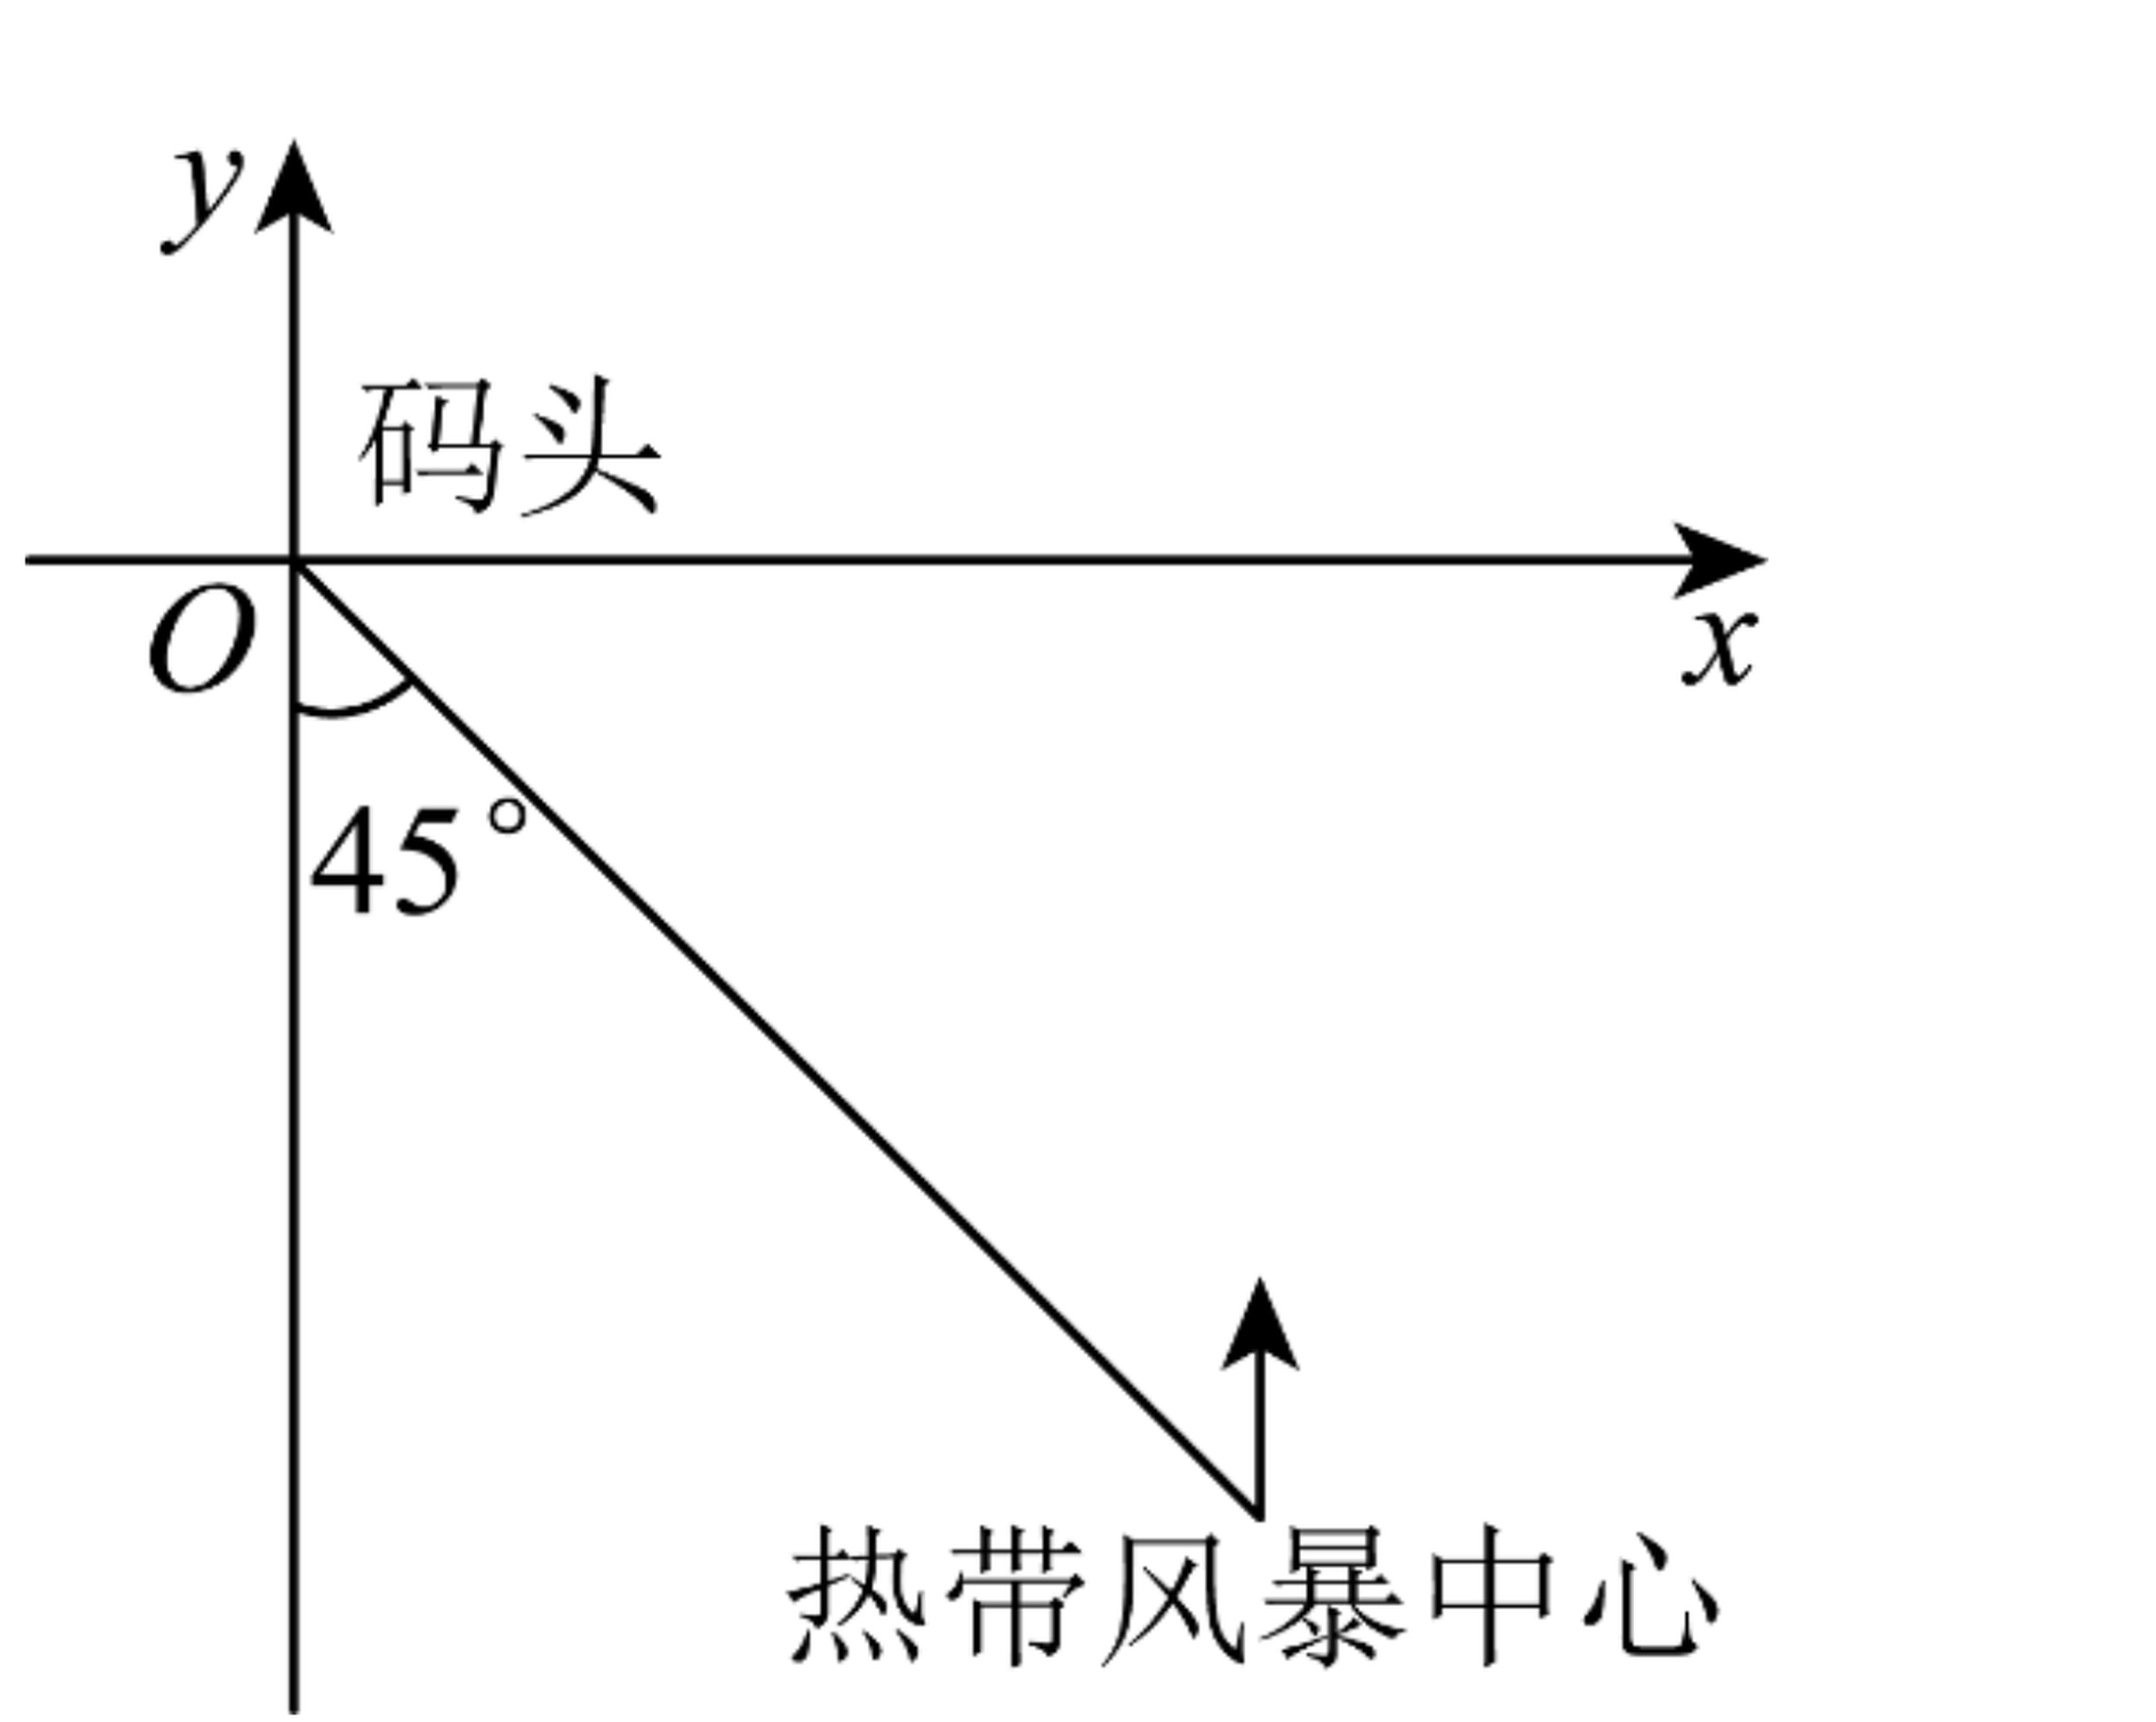
\includegraphics[width=0.36\textwidth]{figures/gao123_q5.png}
\end{center}

\ifanswer
\solbegin
\step{设风暴中心的坐标为 $(a,b)$，}
\step{由题意得 $a=400\sqrt2\times\cos45^\circ=400$，当 $a^2+b^2=400^2+b^2<500^2$，}% 原卷 $a^2$ 与 $400^2$ 并用，照录
\step{即 $-300<b<300$ 时，码头将受到风暴影响，}
\step{$\dfrac{300-(-300)}{20}=30h$，则码头受到风暴影响的时长为 30 小时，}
\step{所以由预报估计，该码头将受到热带风暴的影响时长大约为 30 小时.}
\solend
\fi

\item 已知 $a$、$b$、$c$ 为常数，若不等式 $\dfrac{ax-b}{x-c}\geqslant0$ 的解集为 $[-1,1)$，则不等式 $ax+b<0$ 的解集为\blankline[4.4em].

\ifanswer
\solbegin
\step{不等式 $\dfrac{ax-b}{x-c}\geqslant0$ 可化为 $(ax-b)(x-c)\geqslant0$ 且 $x-c\neq0$，}
\step{即 $a\left(x-\dfrac ba\right)(x-c)\geqslant0$ 且 $x\neq c$，}
\step{因为不等式 $\dfrac{ax-b}{x-c}\geqslant0$ 的解集为 $[-1,1)$，所以 $a<0$，且 $\dfrac ba=-1$,$c=1$，}
\step{即 $b=-a$，所以不等式 $ax+b<0$ 可化为 $ax-a<0$，又因为 $a<0$，所以 $x-1>0$，}
\step{解得 $x>1$，所以不等式 $ax+b<0$ 的解集为 $(1,+\infty)$.}
\solend
\fi

\item 已知实数 $a$、$b$ 满足 $ab=32$，且 $\log_2a=\log_b16$，则 $a+b$ 的值为\blankline[4.4em].

\ifanswer
\solbegin
\step{由 $\log_2a=\log_b16$，得 $\log_2a=\dfrac{\log_216}{\log_2b}$，则 $\log_2a\cdot\log_2b=4$，}
\step{由 $ab=32$，得 $\log_2a+\log_2b=\log_2ab=5$，}
\step{得 $\log_2a=1$,$\log_2b=4$ 或 $\log_2a=4$,$\log_2b=1$，}
\step{因此 $a=2$,$b=16$ 或 $a=16$,$b=2$，所以 $a+b=18$.}
\solend
\fi

\item 已知实数 $a$、$b$ 满足 $-3<a+2b<2$，$-1<2a-b<4$，则 $a+b$ 的取值范围为\blankline[4.4em].

\ifanswer
\solbegin
\step{设 $a+b=m(a+2b)+n(2a-b)=(m+2n)a+(2m-n)b$，}
\step{所以 $\begin{cases}m+2n=1\\2m-n=1\end{cases}$，解得 $n=\dfrac15$,$m=\dfrac35$，所以 $a+b=\dfrac35(a+2b)+\dfrac15(2a-b)$，}
\step{因为 $-3<(a+2b)<2$，$-1<2a-b<4$，}
\step{所以 $-\dfrac95<\dfrac35(a+2b)<\dfrac65$，$-\dfrac15<\dfrac15(2a-b)<\dfrac45$，}
\step{相加得 $-2<\dfrac35(a+2b)+\dfrac15(2a-b)<2$，即 $-2<a+b<2$，}
\step{故 $a+b$ 的取值范围为 $(-2,2)$.}
\solend
\fi

\item 存在 $x\in\R$ 使不等式 $\lvert2x-a\rvert<\lvert2a-1\rvert-2\lvert x\rvert$ 成立，则实数 $a$ 的取值范围是\blankline[4.4em].

\ifanswer
\solbegin
\step{存在 $x\in\R$，不等式 $\lvert2x-a\rvert<\lvert2a-1\rvert-2\lvert x\rvert$ 成立，}
\step{变形即 $\lvert2x-a\rvert+2\lvert x\rvert<\lvert2a-1\rvert$ 成立，}
\step{由于 $\lvert2x-a\rvert+\lvert2x\rvert\geqslant\lvert(2x-a)-2x\rvert=\lvert a\rvert$，当且仅当 $2x(2x-a)\leqslant0$ 时取等号，}
\step{因此有 $\lvert a\rvert<\lvert2a-1\rvert$，两边平方 $a^2<(2a-1)^2$，解得 $a>1$ 得 $a<\dfrac13$，}% 原卷“解得 a>1 得 a<1/3”，照录
\step{即实数 $a$ 的取值范围是 $\left(-\infty,\dfrac13\right)\cup(1,+\infty)$.}
\solend
\fi

\item 已知集合 $A=\{(x,y)\mid x^2+mx-y+2=0\}$，$B=\{(x,y)\mid x-y+1=0,0\leqslant x\leqslant3\}$，若集合 $A\cap B$ 的子集个数为 $2$，则实数 $m$ 的取值范围为\blankline[4.4em].

\ifanswer
\solbegin
\step{因为集合 $A\cap B$ 的子集个数为 $2$，所以 $A\cap B$ 的元素有一个，}
\step{即 $\begin{cases}x^2+mx-y+2=0\\x-y+1=0\end{cases}$ 在 $x\in[0,3]$ 上只有一个解，}
\step{即 $x^2+(m-1)x+1=0$ 在 $[0,3]$ 上只有一个解，}
\step{即 $1-m=x+\dfrac1x$ 在 $[0,3]$ 上只有一个解，}
\step{结合对勾函数的性质得 $1-m=2$ 或 $1-m>\dfrac{10}{3}$，解得 $m=-1$ 或 $m<-\dfrac73$.}
\solend
\fi

\item $[x]$ 表示不超过 $x$ 的最大整数，则集合 $A=\left\{y\,\middle\vert\,y=\left[\dfrac{x^2}{100}\right],x=1,2,3,\cdots,100\right\}$ 中的元素个数为\blankline[4.4em].

\ifanswer
\solbegin
\step{记 $a_k=\left[\dfrac{k^2}{100}\right](k=1,2,\cdots,100)$，$a_k$ 随 $k$ 增大而单调不减.}
\step{当 $k\geqslant50$ 时，$\dfrac{(k+1)^2}{100}-\dfrac{k^2}{100}=\dfrac{2k+1}{100}\geqslant\dfrac{101}{100}>1$，所以 $a_{k+1}\geqslant a_k+1$，}
\step{即 $a_{50}$、$a_{51}$、$\cdots$、$a_{100}$ 两两互异.}
\step{又 $a_{50}=\left[\dfrac{2500}{100}\right]=25$、$a_{100}=100$，这一段共 $100-50+1=51$ 个互异的值，}
\step{且都大于等于 $25$.}
\step{当 $k\leqslant49$ 时，$\dfrac{(k+1)^2}{100}-\dfrac{k^2}{100}=\dfrac{2k+1}{100}\leqslant\dfrac{99}{100}<1$，即 $a_k$ 每次至多增加 $1$；}
\step{又 $a_1=0$、$a_{49}=\left[\dfrac{2401}{100}\right]=24$，}
\step{故 $a_1$、$a_2$、$\cdots$、$a_{49}$ 依次取遍 $0$，$1$，$2$，$\cdots$，$24$，共 $25$ 个值.}
\step{两段取值范围互不重叠（前段不超过 $24$、后段不小于 $25$），}
\step{所以集合 $A$ 中共有 $25+51=76$ 个元素.}
\solend
\fi

\item 若实数 $a$、$b$、$c$ 满足 $\dfrac1{2^a}+\dfrac1{2^b}=1$，$\dfrac1{2^{a+b}}+\dfrac1{2^{b+c}}+\dfrac1{2^{a+c}}=1$，则 $c$ 的最大值是\blankline[4.4em].

\ifanswer
\solbegin
\step{因为 $\dfrac1{2^a}+\dfrac1{2^b}=1$，}
\step{由基本不等式得 $1=\dfrac1{2^a}+\dfrac1{2^b}\geqslant2\sqrt{\dfrac1{2^a}\cdot\dfrac1{2^b}}$（当且仅当 $a=b=1$ 时取等号），}
\step{所以 $\dfrac1{2^a}\cdot\dfrac1{2^b}\leqslant\dfrac14$，所以 $-\dfrac1{2^a}\cdot\dfrac1{2^b}\geqslant-\dfrac14$，}% 原卷带负号起论，照录
\step{因为 $\dfrac1{2^{a+b}}+\dfrac1{2^{b+c}}+\dfrac1{2^{a+c}}=1$，$\dfrac1{2^{b+c}}+\dfrac1{2^{a+c}}=\dfrac1{2^c}\left(\dfrac1{2^a}+\dfrac1{2^b}\right)=\dfrac1{2^c}$，}
\step{所以 $\dfrac1{2^c}=1-\dfrac1{2^{a+b}}\geqslant\dfrac34$，所以 $2^c\leqslant\dfrac43$，所以 $c\leqslant\log_2\dfrac43=2-\log_23$，}
\step{故 $c$ 的最大值是 $2-\log_23$.}
\solend
\fi

\end{enumerate}

\bigsec{二、选择题}

\begin{enumerate}
\setcounter{enumi}{12}

\item 下列运用等式或不等式的性质变形中，正确的是\mbox{（\quad）}

\keepwithprev
A. 如果 $a=b$，那么 $\dfrac ac=\dfrac bc$\qquad\qquad B. 如果 $\dfrac1a<\dfrac1b<0$，那么 $a-\dfrac1a>b-\dfrac1b$

C. 如果 $a>b$，那么 $\dfrac1a<\dfrac1b$\qquad\qquad D. 如果 $a>b>0$，$m\in\R$，那么 $\dfrac ba<\dfrac{b+m}{a+m}$

\ifanswer
\solbegin
\step{对于 $A$，若 $c=0$，$A$ 错误；}
\step{对于 $B$，若 $\dfrac1a<\dfrac1b<0$，则 $0>a>b$，$-\dfrac1a>-\dfrac1b>0$，}
\step{所以 $a-\dfrac1a>b-\dfrac1b$，$B$ 正确；}
\step{对于 $C$，$a>0$，$b<0$ 时，$C$ 错误；}
\step{对于 $D$，$\dfrac{b+m}{a+m}-\dfrac ba=\dfrac{ab+am}{a(a+m)}-\dfrac{ab+bm}{a(a+m)}=\dfrac{(a-b)m}{a(a+m)}$，}
\step{因为 $a>b>0$，所以 $a-b>0$，但 $m$、$a+m$ 的符号不确定，}
\step{当 $m=0$ 时，$\dfrac ba=\dfrac{b+m}{a+m}$，}
\step{当 $m(a+m)>0$ 时，$\dfrac ba<\dfrac{b+m}{a+m}$，当 $m(a+m)<0$ 时，$\dfrac ba>\dfrac{b+m}{a+m}$，$D$ 错误.}
\step{故选 $B$.}
\solend
\fi

\item “$a>b$”的一个必要非充分条件是\mbox{（\quad）}

\keepwithprev
A. $ac^2>bc^2$\qquad\quad B. $2^a>2^b$\qquad\quad C. $\left(\dfrac12\right)^{a-b}\leqslant1$\qquad\quad D. $a^3>b^3$

\ifanswer
\solbegin
\step{即“$a>b$”能推出选项，但选项不能推出“$a>b$”，故选 $C$.}
\solend
\fi

\item 若 $A=\left\{x\,\middle\vert\,x=\dfrac k6+1,k\in\Z\right\}$，$B=\left\{x\,\middle\vert\,x=\dfrac k3+\dfrac12,k\in\Z\right\}$，$C=\left\{x\,\middle\vert\,x=\dfrac{2k}{3}+\dfrac12,k\in\Z\right\}$，则这三个集合间的关系是\mbox{（\quad）}

\keepwithprev
A. $A\subseteq B\subseteq C$\qquad\quad B. $A\subseteq C\subseteq B$\qquad\quad C. $C\subseteq B\subseteq A$\qquad\quad D. $C\subseteq A\subseteq B$

\ifanswer
\solbegin
\step{若 $x\in C$，则存在 $k_0\in\Z$，使 $x=\dfrac{2k_0}{3}+\dfrac12$，}
\step{又 $2k_0\in\Z$，所以 $x\in B$，故 $C\subseteq B$，}
\step{若 $x\in B$，则存在 $k_1\in\Z$，使 $x=\dfrac{k_1}{3}+\dfrac12=\dfrac{2k_1-3}{6}+1$，}
\step{又 $2k_1-3\in\Z$，所以 $x\in A$，故 $B\subseteq A$，}
\step{又 $\dfrac43\in A$，$\dfrac43\notin B$，$\dfrac56\in B$，$\dfrac56\notin C$，所以 $C\subseteq B\subseteq A$，故选 $C$.}
\solend
\fi

\item 集合 $S=\{x\mid(x+a)(x^2+bx+c)=0\}$，$T=\{x\mid(ax+1)(cx^2+bx+1)=0\}$，其中 $a$、$b$、$c$ 为实数，若 $\lvert S\rvert$、$\lvert T\rvert$ 分别表示 $S$、$T$ 的元素个数，则下列结论中一定成立的是\mbox{（\quad）}

\keepwithprev
A. 若 $\lvert T\rvert=0$，则 $\lvert S\rvert=1$\qquad\qquad B. 若 $\lvert S\rvert=1$，则 $\lvert T\rvert=1$

C. 若 $\lvert S\rvert=2$，则 $\lvert T\rvert=2$\qquad\qquad D. 若 $\lvert T\rvert=3$，则 $\lvert S\rvert=2$

\ifanswer
\solbegin
\step{令 $f(x)=(x+a)(x^2+bx+c)$,$g(x)=(ax+1)(cx^2+bx+1)$，}
\step{对于选项 A，当 $\lvert T\rvert=0$ 时，方程 $g(x)=(ax+1)(cx^2+bx+1)=0$ 无实根，}
\step{当 $a=b=c=0$ 时，$f(x)=x^3$，由 $f(x)=0$ 得 $x=0$，此时 $\lvert S\rvert=1$；}
\step{当 $a=0$,$b^2-4c<0$ 时，$f(x)=x(x^2+bx+c)$，由 $f(x)=0$ 得 $x=0$，}
\step{此时 $\lvert S\rvert=1$，所以选项 A 正确；}
\step{对于选项 B，若 $\lvert S\rvert=1$，则 $f(x)=(x+a)(x^2+bx+c)=0$ 有且只有一根，}
\step{又 $x=-a$ 一定是 $f(x)=0$ 的根，所以 $\triangle=b^2-4c<0$，}
\step{又 $\triangle=b^2-4c<0$ 且 $a=0$ 时，$g(x)=(ax+1)(cx^2+bx+1)=0$ 无解，}
\step{此时 $\lvert T\rvert=0$，所以选项 B 错误，}
\step{对于选项 C，若 $\lvert S\rvert=2$ 时，则 $f(x)=(x+a)(x^2+bx+c)=0$ 有且只有 $2$ 根，}
\step{又 $x=-a$ 一定是 $f(x)=0$ 的根，}
\step{所以 $\triangle=b^2-4c=0$ 且 $a^2+ab+c\neq0$ 或 $\triangle=b^2-4c>0$ 且 $a^2+ab+c=0$，}
\step{当 $a=0$ 时，存在 $b$,$c$，使 $\triangle=b^2-4c=0$ 且 $a^2+ab+c\neq0$，}
\step{此时 $g(x)=(ax+1)(cx^2+bx+1)=0$ 只有一根，所以选项 C 错误，}
\step{对于选项 D，当 $\lvert T\rvert=3$ 时，方程 $g(x)=(ax+1)(cx^2+bx+1)=0$ 有三个根，}
\step{所以 $a\neq0$,$c\neq0$,$b^2-4c>0$，}
\step{设 $x_0$ 为 $g(x)=0$ 的一个根，即 $(ax_0+1)(cx_0^2+bx_0+1)=0$，}
\step{则 $x_0\neq0$，且 $f\left(\dfrac1{x_0}\right)=\left(\dfrac1{x_0}+a\right)\left(\dfrac1{x_0^2}+\dfrac1{x_0}b+c\right)=\dfrac1{x_0^3}g(x_0)=0$，}
\step{所以 $\dfrac1{x_0}$ 为方程 $f(x)=0$ 的根，故 $f(x)=0$ 有三个根，即 $\lvert T\rvert=3$ 时，}
\step{必有 $\lvert S\rvert=3$，所以选项 D 错误，}
\step{故选 $A$.}
\solend
\fi

\end{enumerate}

% 第 17 题是解答题第一题且带文氏图，守卫放在 \bigsec 之前，连节标题一起量页高
\needvspace{7cm}
\bigsec{三、解答题}

\begin{enumerate}
\setcounter{enumi}{16}

\item 设全集 $U=\R$，集合 $A=\{x\mid-2\leqslant x\leqslant4\}$，$B=\{x\mid x<-6$ 或 $x\geqslant2\}$.

（1）求图中阴影部分表示的集合；

（2）已知集合 $C=\{x\mid10-a<x<2a+1\}$，若 $\overline B\cap C=\varnothing$，求 $a$ 的取值范围.

\begin{center}
% 图取原卷截图（第 7 页题干右侧）、去水印后 2× LANCZOS 放大，本稿移至题干之后
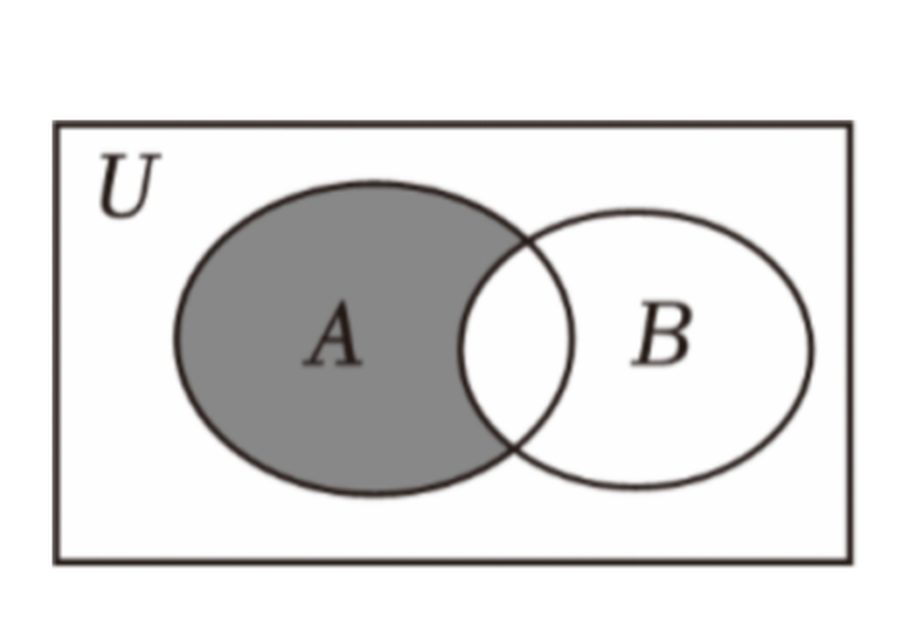
\includegraphics[width=0.34\textwidth]{figures/gao123_q17.png}
\end{center}

\ifanswer
\solbegin
\step{（1）$A\cap B=\{x\mid2\leqslant x\leqslant4\}$，}
\step{则图中阴影部分表示 $\overline{A\cap B}=\{x\mid-2\leqslant x<2\}$.}% 原卷把上划线盖在整个 $A\cap B$ 上，照录
\step{（2）由题意得 $\overline B=\{x\mid-6\leqslant x<2\}$，$C\subseteq B$，}
\step{所以当 $C=\varnothing$ 时，$10-a\geqslant2a+1$，解得 $a\leqslant3$，符合题意；}
\step{当 $C\neq\varnothing$ 时，$\begin{cases}10-a<2a+1\\2a+1\leqslant-6\end{cases}$ 或者 $\begin{cases}10-a<2a+1\\10-a\geqslant2\end{cases}$，}
\step{此时不等式组 $\begin{cases}10-a<2a+1\\2a+1\leqslant-6\end{cases}$ 无解，}
\step{不等式组 $\begin{cases}10-a<2a+1\\10-a\geqslant2\end{cases}$ 的解集为 $3<a\leqslant8$，}
\step{综上，$a$ 的取值范围为 $\{a\mid a\leqslant8\}$.}
\solend
\fi

\item (1) 求不等式：$\lvert x-1\rvert+\lvert x-2\rvert\leqslant5$ 的解集.

(2) 当 $m<1$ 时，解关于 $x$ 的不等式 $\dfrac{m(x-3)}{x+2}>1$.

\ifanswer
\solbegin
\step{(1) 当 $x<1$ 时，$\lvert x-1\rvert+\lvert x-2\rvert\leqslant5\Leftrightarrow-x+1+2-x\leqslant5$，}
\step{解得 $-1\leqslant x<1$；}
\step{当 $1\leqslant x\leqslant2$ 时，$\lvert x-1\rvert+\lvert x-2\rvert\leqslant5\Leftrightarrow x-1+2-x=1\leqslant5$ 恒成立，}
\step{所以 $1\leqslant x\leqslant2$；}
\step{当 $x>2$ 时，$\lvert x-1\rvert+\lvert x-2\rvert\leqslant5\Leftrightarrow x-1+x-2=2x-3\leqslant5$，}
\step{解得 $2<x\leqslant4$.}
\step{综上所述，不等式 $\lvert x-1\rvert+\lvert x-2\rvert\leqslant5$ 的解集为 $[-1,4]$.}
\step{(2) 原不等式变成 $\dfrac{(m-1)x-(3m+2)}{x+2}>0$，$n<1$，所以 $n-1<0$，}% 原卷作 $n<1$、$n-1<0$，与题设 $m<1$ 字母不一致，照录
\step{所以原不等式变成 $\dfrac{x-\dfrac{3m+2}{m-1}}{x+2}<0$，$\dfrac{3m+2}{m-1}-(-2)=\dfrac{5m}{m-1}$，}
\step{所以 $m<0$ 时，$\dfrac{5m}{m-1}>0$，$\dfrac{3m+2}{m-1}>-2$，}
\step{原不等式的解集为 $\left(-2,\dfrac{3m+2}{m-1}\right)$；}
\step{$m=0$ 时，原不等式变成 $1<0$，无解；}
\step{$0<m<1$ 时，$\dfrac{5m}{m-1}<0$，$\dfrac{3m+2}{m-1}<-2$，}
\step{原不等式的解集为 $\left(\dfrac{3m+2}{m-1},-2\right)$.}
\solend
\fi

\item 在园林博览会上，某公司带来了一种智能设备供采购商洽谈采购，并决定大量投放市场，已知该种设备年固定研发成本为 $50$ 万元，每生产一台需另投入 $100$ 元，设该公司一年内生产该设备 $x$ 万台且全部售完，每万台的销售收入 $G(x)$（万元）与年产量 $x$（万台）满足如下关系式：$G(x)=\begin{cases}180-x,0<x\leqslant20\\80+\dfrac{2000}{x}-\dfrac{8000}{x(x-1)},x>20\end{cases}$.

(1) 写出年利润 $W(x)$（万元）关于年产量 $x$（万台）的函数解析式；（利润 $=$ 销售收入 $-$ 成本）

(2) 当年产量为多少万台时，该公司获得的年利润最大，并求出最大利润.

\ifanswer
\solbegin
\step{(1) $W(x)=xG(x)-50-100x=\begin{cases}-50+80x-x^2,0<x\leqslant20\\-20x+1950-\dfrac{8000}{x-1},x>20\end{cases}$；}
\step{(2) 当 $0<x\leqslant20$ 时，$W(x)=-50+80x-x^2=-(x-40)^2+1550$，}
\step{由函数性质得当 $x\leqslant40$ 时严格增，所以当 $x=20$ 时，$W(x)_{max}=1150$，}
\step{当 $x>20$ 时，$W(x)=-20x+1950-\dfrac{8000}{x-1}=-20\left[(x-1)+\dfrac{400}{x-1}\right]+1930$，}
\step{$W(x)=-20\left[(x-1)+\dfrac{400}{x-1}\right]+1930\leqslant-20\times2\sqrt{(x-1)\cdot\dfrac{400}{x-1}}+1930$}
\step{$=1130$，当且仅当 $x-1=\dfrac{400}{x-1}$，即 $x=21$ 时取等号，}
\step{所以 $W(x)_{max}=1130$，}
\step{因为 $1150>1130$，所以当 $x=20$ 时，$W(x)_{max}=1150$，}
\step{即当年产量为 $20$ 万台时，该公司获得的年利润最大，}
\step{最大利润为 $1150$ 万元.}
\solend
\fi

\item 关于 $x$ 的方程 $(x^2-1)^2-2k\lvert x^2-1\rvert+k+1=0(k\in\R)$.

(1) 若方程无实根，求 $k$ 的取值范围；

(2) 若方程有 $4$ 个不等实根，求 $k$ 的取值范围；

(3) 若 $k=a+b$，且满足 $\dfrac1{a+2b}+\dfrac1{a+3}=\dfrac12$，$a>0$，$b>0$，试判断方程根的个数.

\ifanswer
\solbegin
\step{(1) 关于 $x$ 的方程 $(x^2-1)^2-2k\lvert x^2-1\rvert+k+1=0(k\in\R)$，}
\step{令 $t=\lvert x^2-1\rvert$，则 $t\geqslant0$，则原方程转化为 $t^2-2kt+k+1=0(*)$，}
\step{因为关于 $x$ 的方程 $(x^2-1)^2-2k\lvert x^2-1\rvert+k+1=0(k\in\R)$ 无实根，}
\step{所以 $(*)$ 式无实根或实根均小于零，令 $f(t)=t^2-2kt+k+1$，}
\step{①若 $(*)$ 式无实根，则 $\triangle<0$，解得 $\dfrac{1-\sqrt5}{2}<k<\dfrac{1+\sqrt5}{2}$，}
\step{②两根均为负，则 $\begin{cases}\Delta\geqslant0\\t_{\text{对}}=k<0\\f(0)>0\end{cases}$，解得 $-1<k\leqslant\dfrac{1-\sqrt5}{2}$，}
\step{综合①②，得 $k$ 的取值范围是 $\left(-1,\dfrac{1+\sqrt5}{2}\right)$；}
\step{(2) 作函数 $t=\lvert x^2-1\rvert$ 的图象，}
\begin{center}
% 图取原卷截图（第 11 页解析内）、去水印后 2× LANCZOS 放大，仅答案版出
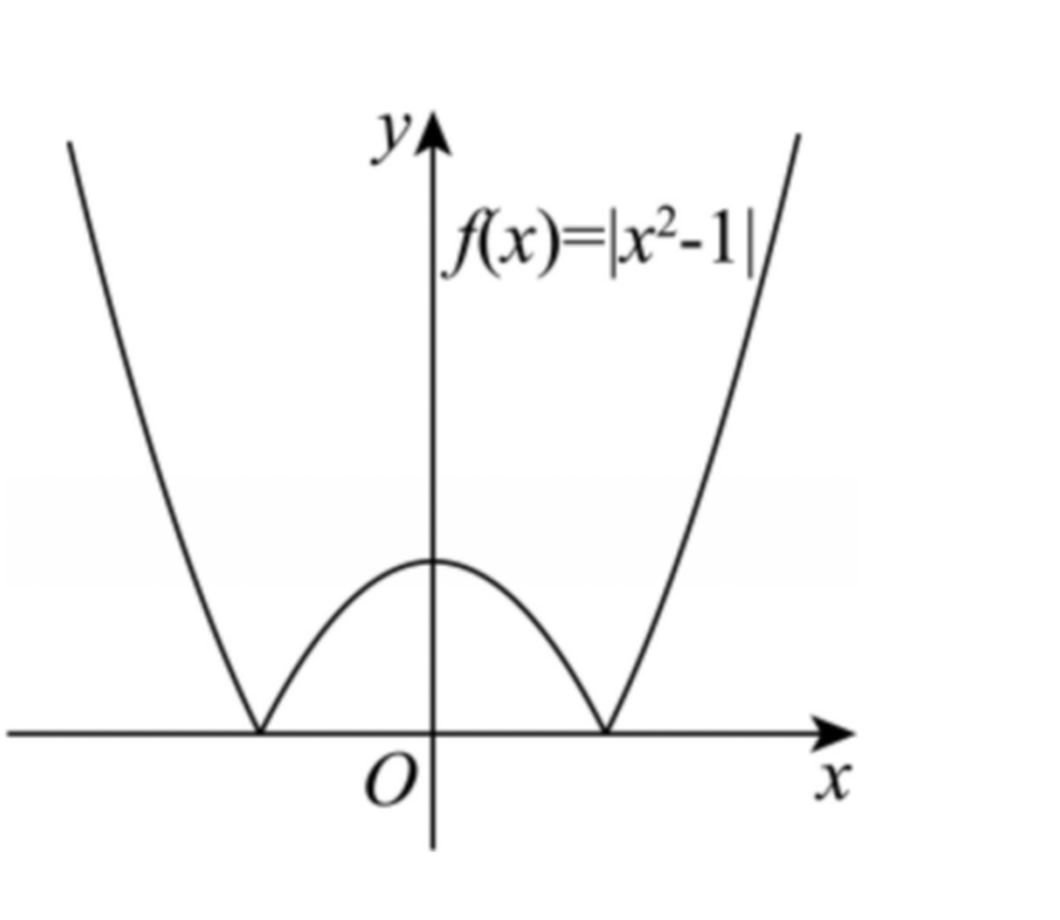
\includegraphics[width=0.40\textwidth]{figures/gao123_q20.png}
\end{center}
\step{$t=0$ 或 $t>1$ 时，每一个 $t$ 值对应 $2$ 个不同的 $x$ 值，}
\step{$t=1$ 时一个 $t$ 值对应 $3$ 个不同的 $x$ 值，}
\step{$0<t<1$ 时一个 $t$ 值对应 $4$ 个不同的 $x$ 值，}
\step{要使原方程有四个不等实根，}
\step{①$(*)$ 式一根为零，另一根大于 $1$，无解；}
\step{②$(*)$ 有两不等根且两根均大于 $1$，则 $\begin{cases}\Delta>0\\t_{\text{对}}=k>1\\f(1)>0\end{cases}$，解得 $\dfrac{1+\sqrt5}{2}<k<2$；}
\step{④$(*)$ 式有 $1$ 实根在 $(0,1)$ 之间，另一根小于零，}% 原卷由 ② 直接跳到 ④，缺 ③，照录
\step{则 $\begin{cases}f(0)<0\\f(1)>0\end{cases}$，所以 $\begin{cases}k+1<0\\2-k>0\end{cases}$，解得 $k<-1$，}
\step{综上所述，$k$ 取值范围为 $(-\infty,-1)\cup\left(\dfrac{1+\sqrt5}{2},2\right)$；}
\step{(3) 因为 $\dfrac1{a+2b}+\dfrac1{a+3}=\dfrac{a+2b+a+3}{(a+2b)(a+3)}=\dfrac{2(a+b)+3}{(a+2b)(a+3)}=\dfrac12$，}
\step{所以 $2(a+b)+3=\dfrac12(a+2b)(a+3)$，}
\step{因为 $a$、$b$ 为正实数，所以 $\dfrac12=\dfrac1{a+2b}+\dfrac1{a+3}\geqslant2\sqrt{\dfrac1{a+2b}\times\dfrac1{a+3}}$，}
\step{得 $\dfrac1{16}\geqslant\dfrac1{a+2b}\times\dfrac1{a+3}$，即 $(a+2b)(a+3)\geqslant16$，}
\step{所以 $2(a+b)+3\geqslant8$，即 $a+b\geqslant\dfrac52$，}
\step{当且仅当 $\dfrac1{a+2b}=\dfrac1{a+3}$ 即 $a=1$,$b=\dfrac32$ 时取等号，}
\step{故 $k\geqslant\dfrac52$，此时有 $\begin{cases}\Delta>0\\t_{\text{对}}=k>1\\f(0)>0,f(1)<0\end{cases}$，}
\step{故 $(*)$ 式有两不等实根且一根在 $(0,1)$ 之间，另一根大于 $1$，}
\step{故原方程有 $6$ 个实根.}
\solend
\fi

\item 设 $n$ 是不小于 $3$ 的正整数，集合 $S_n=\{(a_1,a_2,\cdots,a_n)\mid a_i\in\{0,1\},i=1,2,\cdots,n\}$，对于集合 $S_n$ 中任意两个元素 $A=(a_1,a_2,\cdots,a_n)$，$B=(b_1,b_2,\cdots,b_n)$.

定义 1：$A\cdot B=n-(\lvert a_1-b_1\rvert+\lvert a_2-b_2\rvert+\cdots+\lvert a_n-b_n\rvert)$，

定义 2：若 $A\cdot B=0$，则称互为相反元素，记作 $A=\overline B$ 或 $B=\overline A$.

(1) 若 $n=3$，$A=(0,1,0)$，$B=(1,1,0)$，试写出 $\overline A$、$\overline B$ 以及 $A\cdot B$ 的值；

(2) 若 $A$、$B\in S_n$，$A=(a_1,a_2,\cdots,a_n)$，$B=(b_1,b_2,\cdots,b_n)$，证明：$A\cdot B+\overline A\cdot B=n$；

(3) 设 $k$ 是小于 $n$ 的正奇数，至少含有两个元素的集合 $M\subseteq S_n$，且对于集合 $M$ 中任意两个不相同的元素 $A=(a_1,a_2,\cdots,a_n)$，$B=(b_1,b_2,\cdots,b_n)$，都有 $A\cdot B=n-k$，试求集合 $M$ 中元素个数的所有可能值.

\ifanswer
\solbegin
\step{(1) $\overline A=(1,0,1)$,$\overline B=(0,0,1)$,$\overline A\cdot\overline B=2$；}
\step{(2) 设 $A=(a_1,a_2,\cdots,a_n)$,$B=(b_1,b_2,\cdots,b_n)$,$\overline A=(x_1,x_2,\cdots,x_n)$，}
\step{由 $a_i$、$b_i$、$x_i\in\{0,1\}$，$i=1,2,\cdots,n$，得 $\lvert a_i-x_i\rvert\leqslant1$，$i=1,2,\cdots,n$，}
\step{所以 $\lvert a_1-x_1\rvert+\lvert a_2-x_2\rvert+\cdots+\lvert a_i-x_i\rvert\leqslant n$，}% 原卷末项下标作 $i$，照录
\step{当且仅当 $\lvert a_i-x_i\rvert=1$，$i=1,2,\cdots,n$，}
\step{即 $x_i=1-a_i$，$i=1,2,\cdots,n$ 时取等号.}
\step{由题意得 $A\cdot\overline A=n-(\lvert a_1-x_1\rvert+\lvert a_2-x_2\rvert+\cdots+\lvert a_n-x_n\rvert)=0$，}
\step{即 $\lvert a_1-x_1\rvert+\lvert a_2-x_2\rvert+\cdots+\lvert a_n-x_n\rvert=n$，}
\step{所以 $x_i=1-a_i$，$i=1,2,\cdots,n$，}
\step{$A\cdot B+\overline A\cdot B=2n-\sum\limits_{i=1}^n[\lvert a_i-b_i\rvert+(1-a_i)-b_i]$}
\step{$=2n-\sum\limits_{i=1}^n(\lvert1-b_i\rvert+\lvert0-b_i\rvert)=2n-\sum\limits_{i=1}^n(1-b_i+b_i)=2n-n=n$；}
\step{(3) 假设 $A=(a_1,a_2,\cdots,a_n)$，$B=(b_1,b_2,\cdots,b_n)$，$C=(c_1,c_2,\cdots,c_n)$}
\step{为集合 $M$ 中的三个不相同的元素，}
\step{则 $A\cdot B=n-(\lvert a_1-b_1\rvert+\lvert a_2-b_2\rvert+\cdots+\lvert a_n-b_n\rvert)=n-k$，}
\step{即 $\lvert a_1-b_1\rvert+\lvert a_2-b_2\rvert+\cdots+\lvert a_n-b_n\rvert=k$，}
\step{又由题意得 $\lvert a_i-b_i\rvert=0$ 或 $1$，$i=1,2,\cdots,n$，}
\step{$\lvert a_1-b_1\rvert$、$\lvert a_2-b_2\rvert$、$\cdots$、$\lvert a_n-b_n\rvert$ 恰有 $k$ 个 $1$，$n-k$ 个 $0$，}
\step{设其中 $k$ 个等于 $1$ 的项以此为 $a_{m_1}-b_{m_1}$,$a_{m_2}-b_{m_2}$,$\cdots$,$a_{m_k}-b_{m_k}$，}
\step{$n-k$ 个等于 $0$ 的项为 $a_{m_{k+1}}-b_{m_{k+1}}$,$a_{m_{k+2}}-b_{m_{k+2}}$,$\cdots$,$a_{m_n}-b_{m_n}$，}
\step{由题意得 $A\cdot C=n-(\lvert a_1-c_1\rvert+\lvert a_2-c_2\rvert+\cdots+\lvert a_n-c_n\rvert)=n-k$，}
\step{所以 $\sum\limits_{i=1}^k\lvert a_{m_i}-c_{m_i}\rvert+\sum\limits_{j=k+1}^n\lvert a_{m_j}-c_{m_j}\rvert=k$ ①，}
\step{同理 $\sum\limits_{i=1}^k\lvert b_{m_i}-c_{m_i}\rvert+\sum\limits_{j=k+1}^n\lvert b_{m_j}-c_{m_j}\rvert=k$ ②，}
\step{因为 $\lvert a_{m_{k+1}}-b_{m_{k+1}}\rvert=\lvert a_{m_{k+2}}-b_{m_{k+2}}\rvert=\cdots=\lvert a_{m_n}-b_{m_n}\rvert=0$，}
\step{所以 $\sum\limits_{j=k+1}^n\lvert a_{m_j}-c_{m_j}\rvert=\sum\limits_{j=k+1}^n\lvert b_{m_j}-c_{m_j}\rvert$，}
\step{由①$-$②得 $\sum\limits_{i=1}^k(\lvert a_{m_i}-c_{m_i}\rvert-\lvert b_{m_i}-c_{m_i}\rvert)=0$，}
\step{又 $\sum\limits_{i=1}^k(\lvert a_{m_i}-c_{m_i}\rvert-\lvert b_{m_i}-c_{m_i}\rvert)=\sum\limits_{i=1}^k(\lvert1-c_{m_i}\rvert-\lvert0-c_{m_i}\rvert)=k-2\sum\limits_{i=1}^k c_{m_i}$}
\step{为奇数，与 $\sum\limits_{i=1}^k(\lvert a_{m_i}-c_{m_i}\rvert-\lvert b_{m_i}-c_{m_i}\rvert)=0$ 矛盾，所以假设不成立，}
\step{即集合 $M$ 中至多有两个元素，}
\step{当 $M=\{(1,1,\cdots,1,0,0,\cdots,0),(0,0,\cdots,0)\}$ 时符合题意，}
\step{所以集合 $M$ 中元素的个数只可能是 $2$.}
\solend
\fi

\end{enumerate}

\end{document}
"
% 紧凑版：xelatex "\def\iscompact{1}% 高一123_行知中学_10月月考.tex
%   —— 高一上数学“2026-2027 年行知中学高一上 10 月月考”（试卷版/答案版）
% 试卷版：xelatex 高一123_行知中学_10月月考.tex
% 答案版：xelatex "\def\isanswer{1}\input{高一123_行知中学_10月月考.tex}"
% 紧凑版：xelatex "\def\iscompact{1}\input{高一123_行知中学_10月月考.tex}"
%
% 原始材料：微信公众号“魔都数学加油站”文章，作者破晓，2026-11-09 17:52 发布；
% 连载“27学年高一123”，原文标题“27学年高一123——2026-2027年上海市行知中学高一上10月月考”；
% 原文链接：https://mp.weixin.qq.com/s/GV4SWBLUJrBhMQwo22FVzg。
% 正文为 14 张 PNG 页（第 7、9、11、13、14 页 2560×3620，其余 4762×6735），
% 题目下印有【答案】或【解析】，为讲评版。
% 题目、解析均据原图转录；卷面红色水印及公众号页脚未录入。
% 全卷 3 张插图：第 5 题的坐标示意图、第 17 题的文氏图（均属题干，三版都出）、
% 第 20 题 (2) 的 $t=\lvert x^2-1\rvert$ 图象（属解析，仅答案版出）；
% 都取原卷截图去水印、2× LANCZOS 放大，见 figures/gao123_q5.png、
% figures/gao123_q17.png、figures/gao123_q20.png。
%
% 卷首标题：原卷印作“2026-2027 年行知中学高一上 10 月月考”（公众号标题中的“上海市”
% 卷面标题行没有，本稿照卷面），年份区间按全稿惯例排 en dash；原卷未印副标题，本稿按题目内容
% 标为“集合与常用逻辑用语、不等式”（与 110／111／113／116／118／120 同）。
%
% 与原卷的排版差异：
%   ① 原文从第 3 题起，填空题编号为 3—12、选择题为 13—16、解答题为 17—21，本稿保留原题号；
%   ② 原卷每题下直接印【解析】／【答案】，本稿按全稿惯例置于答案版；第 3 题只印【答案】、
%      另提 \ans{}；选择题答案在解析末句“故选 …”，括号内留空；
%   ③ 原卷未印副标题，本稿按“知识模块”口径补出；
%   ④ 原卷填空横线按全稿惯例排为 \blankline[4.4em]；选择题括号排 \mbox{（\quad）}、
%      选项段前按惯例加 \keepwithprev；解答题不留作答区（原卷为讲评版，与 109—122 同）；
%   ⑤ 原卷数集排斜体 $R$／$Z$（第 9 题作粗体 $\mathbf{R}$），按全稿惯例改 \R／\Z；
%      绝对值按全稿惯例排 \lvert…\rvert，集合描述竖线排 \mid；单位 km、h 原卷排斜体，
%      本稿按正体照排；补集照原卷上划线排 \overline{B}、\overline{A}。
%
% 判别式与子集符号：第 16 题解析的 $\triangle=b^2-4c<0$、第 20 题 (1) ① 的 $\triangle<0$
%   均作等边、扁的 \triangle；第 20 题 ② 两处 cases 与 (3) 的 $\Delta\geqslant0$／$\Delta>0$
%   作等腰、高的 \Delta，逐处照录、不统一；第 15 题选项与第 17 题 (2) 的 $\subseteq$
%   印有下划线，照录 \subseteq。
%
% 原卷存疑照录：
%   第 4 题解析“若 $-\lvert a\rvert=0$，则 $a=0$，则 $A=\{0,-1,0\}$”以元素重复说明互异性；
%   第 5 题解析“当 $a^2+b^2=400^2+b^2<500^2$”等式左边 $a^2$ 与 $400^2$ 并用；
%   第 9 题解析“解得 $a>1$ 得 $a<\dfrac13$”（按平方不等式应为 $a>1$ 或 $a<\dfrac13$）；
%   第 12 题解析“所以 $-\dfrac1{2^a}\cdot\dfrac1{2^b}\geqslant-\dfrac14$”带负号起论；
%   第 17 题 (1) 解析把阴影部分（实为 $A\cap\overline B$）印作 $\overline{A\cap B}$；
%   第 18 题 (2) 解析作“$n<1$，所以 $n-1<0$”，与题设 $m<1$ 字母不一致；
%   第 20 题 (2) 的情形编号由 ①、② 直接跳到 ④（缺 ③）；
%   第 21 题 (2) 解析“$\lvert a_1-x_1\rvert+\cdots+\lvert a_i-x_i\rvert\leqslant n$”
%   末项下标作 $i$（按上下文应为 $n$）。以上均照录加注。
%
% 行数核对：逐题数 \step 条数，合计 176 条（Q3：0；Q4：6；Q5：5；Q6：5；Q7：4；
% Q8：6；Q9：5；Q10：5；Q11：10；Q12：6；Q13：9；Q14：1；Q15：5；Q16：21；
% Q17：8；Q18：14；Q19：10；Q20：26；Q21：30），与原卷印刷行逐题相等
% （cases 块作一个印刷行计）。第 3 题只印【答案】，提 \ans{}，不计入 \step 账。
%
\documentclass[a4paper,11pt]{article}
\usepackage{common}

\begin{document}

\examtitlest[3]{2026--2027 年行知中学高一上 10 月月考}{集合与常用逻辑用语、不等式}

\bigsec{一、填空题}

\begin{enumerate}
\setcounter{enumi}{2}

\item 写出命题“存在实数 $x$、$y$、$z$，使 $x<y$ 或 $y<z$.”的否定\blankline[4.4em].

\ifanswer
\ans{任意实数 $x$、$y$、$z$，使得 $x\geqslant y$ 且 $y\geqslant z$}
\fi

\item 若集合 $\{0,-1,2a\}=\{a-1,-\lvert a\rvert,a+1\}$，实数 $a$ 的值为\blankline[4.4em].

\ifanswer
\solbegin
\step{令 $A=\{0,-1,2a\}$,$B=\{a-1,-\lvert a\rvert,a+1\}$，}
\step{因为 $\{0,-1,2a\}=\{a-1,-\lvert a\rvert,a+1\}$，}
\step{若 $a-1=0$，则 $a=1$，则 $A=\{0,-1,2\}$,$B=\{0,-1,2\}$，满足要求；}
\step{若 $-\lvert a\rvert=0$，则 $a=0$，则 $A=\{0,-1,0\}$，不满足集合元素的互异性；}% 原卷以 $A=\{0,-1,0\}$ 说明互异性，照录
\step{若 $a+1=0$，则 $a=-1$，则 $A=\{0,-1,-2\}$,$B=\{0,-1,-2\}$，满足要求；}
\step{故实数 $a$ 的值为 $\pm1$.}
\solend
\fi

\needvspace{7cm}
\item 如图，据气象部门预报，在距离某码头南偏东 $45^\circ$ 方向 $400\sqrt2$ km 处的热带
风暴中心正在以 $20$km/h 的速度向正北方向移动，距风暴中心 $500$km 以内
的地区都将受到影响. 以上预报估计，该码头将受到热带风暴的影响时长大
约为\blankline[4.4em]$h$.

\begin{center}
% 图取原卷截图（第 1 页题干右侧）、去水印后 2× LANCZOS 放大，本稿移至题干之后
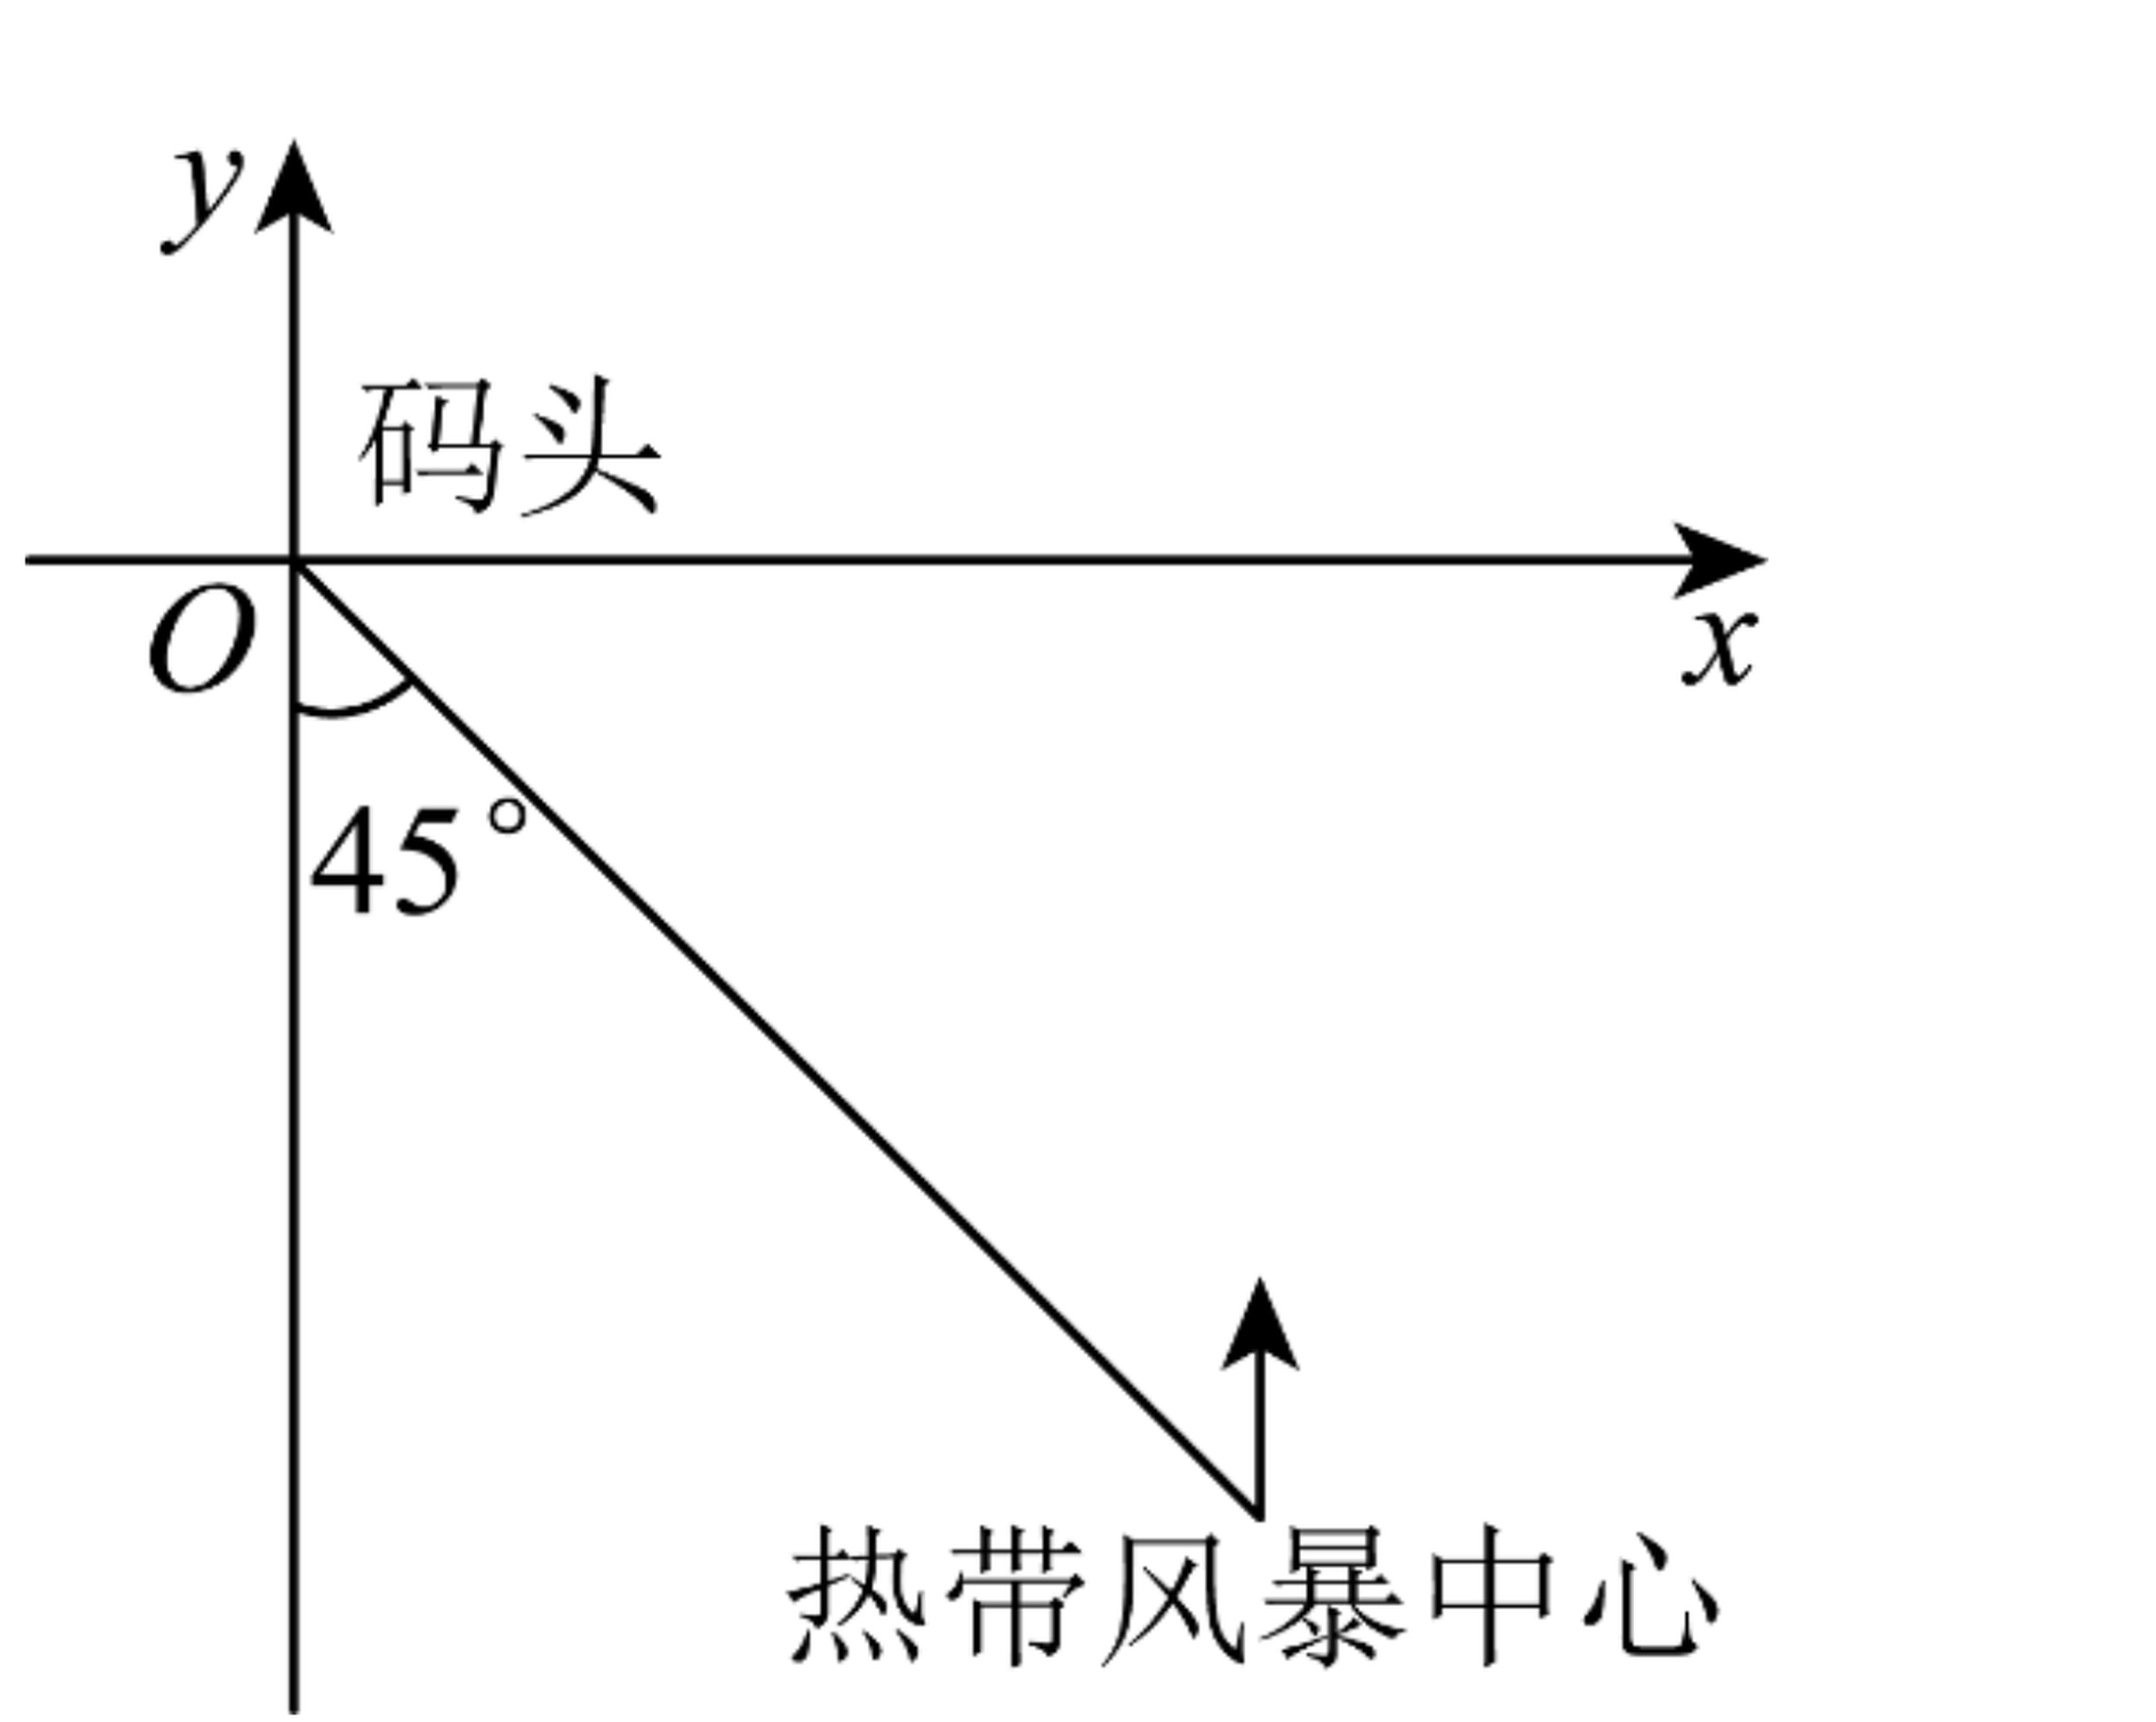
\includegraphics[width=0.36\textwidth]{figures/gao123_q5.png}
\end{center}

\ifanswer
\solbegin
\step{设风暴中心的坐标为 $(a,b)$，}
\step{由题意得 $a=400\sqrt2\times\cos45^\circ=400$，当 $a^2+b^2=400^2+b^2<500^2$，}% 原卷 $a^2$ 与 $400^2$ 并用，照录
\step{即 $-300<b<300$ 时，码头将受到风暴影响，}
\step{$\dfrac{300-(-300)}{20}=30h$，则码头受到风暴影响的时长为 30 小时，}
\step{所以由预报估计，该码头将受到热带风暴的影响时长大约为 30 小时.}
\solend
\fi

\item 已知 $a$、$b$、$c$ 为常数，若不等式 $\dfrac{ax-b}{x-c}\geqslant0$ 的解集为 $[-1,1)$，则不等式 $ax+b<0$ 的解集为\blankline[4.4em].

\ifanswer
\solbegin
\step{不等式 $\dfrac{ax-b}{x-c}\geqslant0$ 可化为 $(ax-b)(x-c)\geqslant0$ 且 $x-c\neq0$，}
\step{即 $a\left(x-\dfrac ba\right)(x-c)\geqslant0$ 且 $x\neq c$，}
\step{因为不等式 $\dfrac{ax-b}{x-c}\geqslant0$ 的解集为 $[-1,1)$，所以 $a<0$，且 $\dfrac ba=-1$,$c=1$，}
\step{即 $b=-a$，所以不等式 $ax+b<0$ 可化为 $ax-a<0$，又因为 $a<0$，所以 $x-1>0$，}
\step{解得 $x>1$，所以不等式 $ax+b<0$ 的解集为 $(1,+\infty)$.}
\solend
\fi

\item 已知实数 $a$、$b$ 满足 $ab=32$，且 $\log_2a=\log_b16$，则 $a+b$ 的值为\blankline[4.4em].

\ifanswer
\solbegin
\step{由 $\log_2a=\log_b16$，得 $\log_2a=\dfrac{\log_216}{\log_2b}$，则 $\log_2a\cdot\log_2b=4$，}
\step{由 $ab=32$，得 $\log_2a+\log_2b=\log_2ab=5$，}
\step{得 $\log_2a=1$,$\log_2b=4$ 或 $\log_2a=4$,$\log_2b=1$，}
\step{因此 $a=2$,$b=16$ 或 $a=16$,$b=2$，所以 $a+b=18$.}
\solend
\fi

\item 已知实数 $a$、$b$ 满足 $-3<a+2b<2$，$-1<2a-b<4$，则 $a+b$ 的取值范围为\blankline[4.4em].

\ifanswer
\solbegin
\step{设 $a+b=m(a+2b)+n(2a-b)=(m+2n)a+(2m-n)b$，}
\step{所以 $\begin{cases}m+2n=1\\2m-n=1\end{cases}$，解得 $n=\dfrac15$,$m=\dfrac35$，所以 $a+b=\dfrac35(a+2b)+\dfrac15(2a-b)$，}
\step{因为 $-3<(a+2b)<2$，$-1<2a-b<4$，}
\step{所以 $-\dfrac95<\dfrac35(a+2b)<\dfrac65$，$-\dfrac15<\dfrac15(2a-b)<\dfrac45$，}
\step{相加得 $-2<\dfrac35(a+2b)+\dfrac15(2a-b)<2$，即 $-2<a+b<2$，}
\step{故 $a+b$ 的取值范围为 $(-2,2)$.}
\solend
\fi

\item 存在 $x\in\R$ 使不等式 $\lvert2x-a\rvert<\lvert2a-1\rvert-2\lvert x\rvert$ 成立，则实数 $a$ 的取值范围是\blankline[4.4em].

\ifanswer
\solbegin
\step{存在 $x\in\R$，不等式 $\lvert2x-a\rvert<\lvert2a-1\rvert-2\lvert x\rvert$ 成立，}
\step{变形即 $\lvert2x-a\rvert+2\lvert x\rvert<\lvert2a-1\rvert$ 成立，}
\step{由于 $\lvert2x-a\rvert+\lvert2x\rvert\geqslant\lvert(2x-a)-2x\rvert=\lvert a\rvert$，当且仅当 $2x(2x-a)\leqslant0$ 时取等号，}
\step{因此有 $\lvert a\rvert<\lvert2a-1\rvert$，两边平方 $a^2<(2a-1)^2$，解得 $a>1$ 得 $a<\dfrac13$，}% 原卷“解得 a>1 得 a<1/3”，照录
\step{即实数 $a$ 的取值范围是 $\left(-\infty,\dfrac13\right)\cup(1,+\infty)$.}
\solend
\fi

\item 已知集合 $A=\{(x,y)\mid x^2+mx-y+2=0\}$，$B=\{(x,y)\mid x-y+1=0,0\leqslant x\leqslant3\}$，若集合 $A\cap B$ 的子集个数为 $2$，则实数 $m$ 的取值范围为\blankline[4.4em].

\ifanswer
\solbegin
\step{因为集合 $A\cap B$ 的子集个数为 $2$，所以 $A\cap B$ 的元素有一个，}
\step{即 $\begin{cases}x^2+mx-y+2=0\\x-y+1=0\end{cases}$ 在 $x\in[0,3]$ 上只有一个解，}
\step{即 $x^2+(m-1)x+1=0$ 在 $[0,3]$ 上只有一个解，}
\step{即 $1-m=x+\dfrac1x$ 在 $[0,3]$ 上只有一个解，}
\step{结合对勾函数的性质得 $1-m=2$ 或 $1-m>\dfrac{10}{3}$，解得 $m=-1$ 或 $m<-\dfrac73$.}
\solend
\fi

\item $[x]$ 表示不超过 $x$ 的最大整数，则集合 $A=\left\{y\,\middle\vert\,y=\left[\dfrac{x^2}{100}\right],x=1,2,3,\cdots,100\right\}$ 中的元素个数为\blankline[4.4em].

\ifanswer
\solbegin
\step{记 $a_k=\left[\dfrac{k^2}{100}\right](k=1,2,\cdots,100)$，$a_k$ 随 $k$ 增大而单调不减.}
\step{当 $k\geqslant50$ 时，$\dfrac{(k+1)^2}{100}-\dfrac{k^2}{100}=\dfrac{2k+1}{100}\geqslant\dfrac{101}{100}>1$，所以 $a_{k+1}\geqslant a_k+1$，}
\step{即 $a_{50}$、$a_{51}$、$\cdots$、$a_{100}$ 两两互异.}
\step{又 $a_{50}=\left[\dfrac{2500}{100}\right]=25$、$a_{100}=100$，这一段共 $100-50+1=51$ 个互异的值，}
\step{且都大于等于 $25$.}
\step{当 $k\leqslant49$ 时，$\dfrac{(k+1)^2}{100}-\dfrac{k^2}{100}=\dfrac{2k+1}{100}\leqslant\dfrac{99}{100}<1$，即 $a_k$ 每次至多增加 $1$；}
\step{又 $a_1=0$、$a_{49}=\left[\dfrac{2401}{100}\right]=24$，}
\step{故 $a_1$、$a_2$、$\cdots$、$a_{49}$ 依次取遍 $0$，$1$，$2$，$\cdots$，$24$，共 $25$ 个值.}
\step{两段取值范围互不重叠（前段不超过 $24$、后段不小于 $25$），}
\step{所以集合 $A$ 中共有 $25+51=76$ 个元素.}
\solend
\fi

\item 若实数 $a$、$b$、$c$ 满足 $\dfrac1{2^a}+\dfrac1{2^b}=1$，$\dfrac1{2^{a+b}}+\dfrac1{2^{b+c}}+\dfrac1{2^{a+c}}=1$，则 $c$ 的最大值是\blankline[4.4em].

\ifanswer
\solbegin
\step{因为 $\dfrac1{2^a}+\dfrac1{2^b}=1$，}
\step{由基本不等式得 $1=\dfrac1{2^a}+\dfrac1{2^b}\geqslant2\sqrt{\dfrac1{2^a}\cdot\dfrac1{2^b}}$（当且仅当 $a=b=1$ 时取等号），}
\step{所以 $\dfrac1{2^a}\cdot\dfrac1{2^b}\leqslant\dfrac14$，所以 $-\dfrac1{2^a}\cdot\dfrac1{2^b}\geqslant-\dfrac14$，}% 原卷带负号起论，照录
\step{因为 $\dfrac1{2^{a+b}}+\dfrac1{2^{b+c}}+\dfrac1{2^{a+c}}=1$，$\dfrac1{2^{b+c}}+\dfrac1{2^{a+c}}=\dfrac1{2^c}\left(\dfrac1{2^a}+\dfrac1{2^b}\right)=\dfrac1{2^c}$，}
\step{所以 $\dfrac1{2^c}=1-\dfrac1{2^{a+b}}\geqslant\dfrac34$，所以 $2^c\leqslant\dfrac43$，所以 $c\leqslant\log_2\dfrac43=2-\log_23$，}
\step{故 $c$ 的最大值是 $2-\log_23$.}
\solend
\fi

\end{enumerate}

\bigsec{二、选择题}

\begin{enumerate}
\setcounter{enumi}{12}

\item 下列运用等式或不等式的性质变形中，正确的是\mbox{（\quad）}

\keepwithprev
A. 如果 $a=b$，那么 $\dfrac ac=\dfrac bc$\qquad\qquad B. 如果 $\dfrac1a<\dfrac1b<0$，那么 $a-\dfrac1a>b-\dfrac1b$

C. 如果 $a>b$，那么 $\dfrac1a<\dfrac1b$\qquad\qquad D. 如果 $a>b>0$，$m\in\R$，那么 $\dfrac ba<\dfrac{b+m}{a+m}$

\ifanswer
\solbegin
\step{对于 $A$，若 $c=0$，$A$ 错误；}
\step{对于 $B$，若 $\dfrac1a<\dfrac1b<0$，则 $0>a>b$，$-\dfrac1a>-\dfrac1b>0$，}
\step{所以 $a-\dfrac1a>b-\dfrac1b$，$B$ 正确；}
\step{对于 $C$，$a>0$，$b<0$ 时，$C$ 错误；}
\step{对于 $D$，$\dfrac{b+m}{a+m}-\dfrac ba=\dfrac{ab+am}{a(a+m)}-\dfrac{ab+bm}{a(a+m)}=\dfrac{(a-b)m}{a(a+m)}$，}
\step{因为 $a>b>0$，所以 $a-b>0$，但 $m$、$a+m$ 的符号不确定，}
\step{当 $m=0$ 时，$\dfrac ba=\dfrac{b+m}{a+m}$，}
\step{当 $m(a+m)>0$ 时，$\dfrac ba<\dfrac{b+m}{a+m}$，当 $m(a+m)<0$ 时，$\dfrac ba>\dfrac{b+m}{a+m}$，$D$ 错误.}
\step{故选 $B$.}
\solend
\fi

\item “$a>b$”的一个必要非充分条件是\mbox{（\quad）}

\keepwithprev
A. $ac^2>bc^2$\qquad\quad B. $2^a>2^b$\qquad\quad C. $\left(\dfrac12\right)^{a-b}\leqslant1$\qquad\quad D. $a^3>b^3$

\ifanswer
\solbegin
\step{即“$a>b$”能推出选项，但选项不能推出“$a>b$”，故选 $C$.}
\solend
\fi

\item 若 $A=\left\{x\,\middle\vert\,x=\dfrac k6+1,k\in\Z\right\}$，$B=\left\{x\,\middle\vert\,x=\dfrac k3+\dfrac12,k\in\Z\right\}$，$C=\left\{x\,\middle\vert\,x=\dfrac{2k}{3}+\dfrac12,k\in\Z\right\}$，则这三个集合间的关系是\mbox{（\quad）}

\keepwithprev
A. $A\subseteq B\subseteq C$\qquad\quad B. $A\subseteq C\subseteq B$\qquad\quad C. $C\subseteq B\subseteq A$\qquad\quad D. $C\subseteq A\subseteq B$

\ifanswer
\solbegin
\step{若 $x\in C$，则存在 $k_0\in\Z$，使 $x=\dfrac{2k_0}{3}+\dfrac12$，}
\step{又 $2k_0\in\Z$，所以 $x\in B$，故 $C\subseteq B$，}
\step{若 $x\in B$，则存在 $k_1\in\Z$，使 $x=\dfrac{k_1}{3}+\dfrac12=\dfrac{2k_1-3}{6}+1$，}
\step{又 $2k_1-3\in\Z$，所以 $x\in A$，故 $B\subseteq A$，}
\step{又 $\dfrac43\in A$，$\dfrac43\notin B$，$\dfrac56\in B$，$\dfrac56\notin C$，所以 $C\subseteq B\subseteq A$，故选 $C$.}
\solend
\fi

\item 集合 $S=\{x\mid(x+a)(x^2+bx+c)=0\}$，$T=\{x\mid(ax+1)(cx^2+bx+1)=0\}$，其中 $a$、$b$、$c$ 为实数，若 $\lvert S\rvert$、$\lvert T\rvert$ 分别表示 $S$、$T$ 的元素个数，则下列结论中一定成立的是\mbox{（\quad）}

\keepwithprev
A. 若 $\lvert T\rvert=0$，则 $\lvert S\rvert=1$\qquad\qquad B. 若 $\lvert S\rvert=1$，则 $\lvert T\rvert=1$

C. 若 $\lvert S\rvert=2$，则 $\lvert T\rvert=2$\qquad\qquad D. 若 $\lvert T\rvert=3$，则 $\lvert S\rvert=2$

\ifanswer
\solbegin
\step{令 $f(x)=(x+a)(x^2+bx+c)$,$g(x)=(ax+1)(cx^2+bx+1)$，}
\step{对于选项 A，当 $\lvert T\rvert=0$ 时，方程 $g(x)=(ax+1)(cx^2+bx+1)=0$ 无实根，}
\step{当 $a=b=c=0$ 时，$f(x)=x^3$，由 $f(x)=0$ 得 $x=0$，此时 $\lvert S\rvert=1$；}
\step{当 $a=0$,$b^2-4c<0$ 时，$f(x)=x(x^2+bx+c)$，由 $f(x)=0$ 得 $x=0$，}
\step{此时 $\lvert S\rvert=1$，所以选项 A 正确；}
\step{对于选项 B，若 $\lvert S\rvert=1$，则 $f(x)=(x+a)(x^2+bx+c)=0$ 有且只有一根，}
\step{又 $x=-a$ 一定是 $f(x)=0$ 的根，所以 $\triangle=b^2-4c<0$，}
\step{又 $\triangle=b^2-4c<0$ 且 $a=0$ 时，$g(x)=(ax+1)(cx^2+bx+1)=0$ 无解，}
\step{此时 $\lvert T\rvert=0$，所以选项 B 错误，}
\step{对于选项 C，若 $\lvert S\rvert=2$ 时，则 $f(x)=(x+a)(x^2+bx+c)=0$ 有且只有 $2$ 根，}
\step{又 $x=-a$ 一定是 $f(x)=0$ 的根，}
\step{所以 $\triangle=b^2-4c=0$ 且 $a^2+ab+c\neq0$ 或 $\triangle=b^2-4c>0$ 且 $a^2+ab+c=0$，}
\step{当 $a=0$ 时，存在 $b$,$c$，使 $\triangle=b^2-4c=0$ 且 $a^2+ab+c\neq0$，}
\step{此时 $g(x)=(ax+1)(cx^2+bx+1)=0$ 只有一根，所以选项 C 错误，}
\step{对于选项 D，当 $\lvert T\rvert=3$ 时，方程 $g(x)=(ax+1)(cx^2+bx+1)=0$ 有三个根，}
\step{所以 $a\neq0$,$c\neq0$,$b^2-4c>0$，}
\step{设 $x_0$ 为 $g(x)=0$ 的一个根，即 $(ax_0+1)(cx_0^2+bx_0+1)=0$，}
\step{则 $x_0\neq0$，且 $f\left(\dfrac1{x_0}\right)=\left(\dfrac1{x_0}+a\right)\left(\dfrac1{x_0^2}+\dfrac1{x_0}b+c\right)=\dfrac1{x_0^3}g(x_0)=0$，}
\step{所以 $\dfrac1{x_0}$ 为方程 $f(x)=0$ 的根，故 $f(x)=0$ 有三个根，即 $\lvert T\rvert=3$ 时，}
\step{必有 $\lvert S\rvert=3$，所以选项 D 错误，}
\step{故选 $A$.}
\solend
\fi

\end{enumerate}

% 第 17 题是解答题第一题且带文氏图，守卫放在 \bigsec 之前，连节标题一起量页高
\needvspace{7cm}
\bigsec{三、解答题}

\begin{enumerate}
\setcounter{enumi}{16}

\item 设全集 $U=\R$，集合 $A=\{x\mid-2\leqslant x\leqslant4\}$，$B=\{x\mid x<-6$ 或 $x\geqslant2\}$.

（1）求图中阴影部分表示的集合；

（2）已知集合 $C=\{x\mid10-a<x<2a+1\}$，若 $\overline B\cap C=\varnothing$，求 $a$ 的取值范围.

\begin{center}
% 图取原卷截图（第 7 页题干右侧）、去水印后 2× LANCZOS 放大，本稿移至题干之后
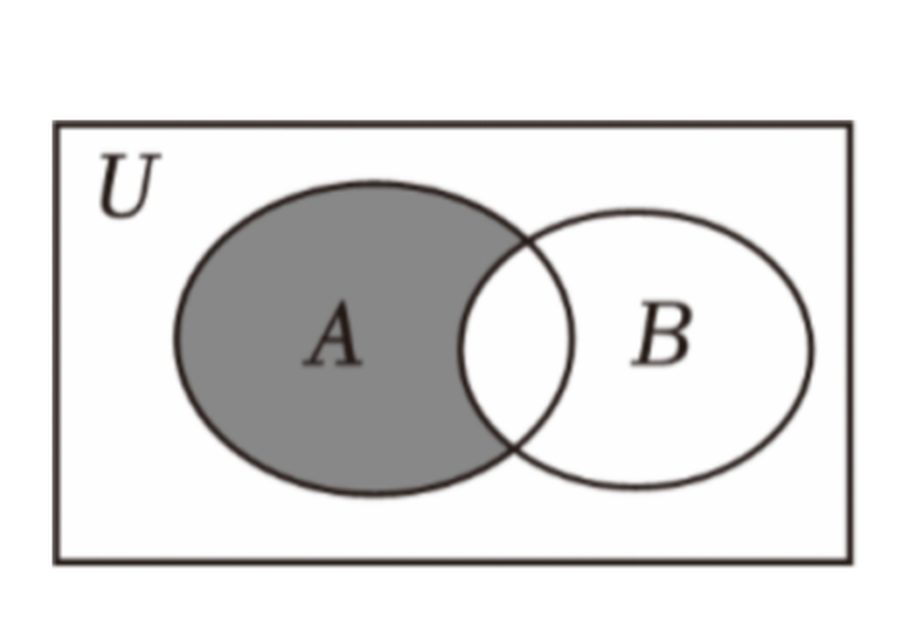
\includegraphics[width=0.34\textwidth]{figures/gao123_q17.png}
\end{center}

\ifanswer
\solbegin
\step{（1）$A\cap B=\{x\mid2\leqslant x\leqslant4\}$，}
\step{则图中阴影部分表示 $\overline{A\cap B}=\{x\mid-2\leqslant x<2\}$.}% 原卷把上划线盖在整个 $A\cap B$ 上，照录
\step{（2）由题意得 $\overline B=\{x\mid-6\leqslant x<2\}$，$C\subseteq B$，}
\step{所以当 $C=\varnothing$ 时，$10-a\geqslant2a+1$，解得 $a\leqslant3$，符合题意；}
\step{当 $C\neq\varnothing$ 时，$\begin{cases}10-a<2a+1\\2a+1\leqslant-6\end{cases}$ 或者 $\begin{cases}10-a<2a+1\\10-a\geqslant2\end{cases}$，}
\step{此时不等式组 $\begin{cases}10-a<2a+1\\2a+1\leqslant-6\end{cases}$ 无解，}
\step{不等式组 $\begin{cases}10-a<2a+1\\10-a\geqslant2\end{cases}$ 的解集为 $3<a\leqslant8$，}
\step{综上，$a$ 的取值范围为 $\{a\mid a\leqslant8\}$.}
\solend
\fi

\item (1) 求不等式：$\lvert x-1\rvert+\lvert x-2\rvert\leqslant5$ 的解集.

(2) 当 $m<1$ 时，解关于 $x$ 的不等式 $\dfrac{m(x-3)}{x+2}>1$.

\ifanswer
\solbegin
\step{(1) 当 $x<1$ 时，$\lvert x-1\rvert+\lvert x-2\rvert\leqslant5\Leftrightarrow-x+1+2-x\leqslant5$，}
\step{解得 $-1\leqslant x<1$；}
\step{当 $1\leqslant x\leqslant2$ 时，$\lvert x-1\rvert+\lvert x-2\rvert\leqslant5\Leftrightarrow x-1+2-x=1\leqslant5$ 恒成立，}
\step{所以 $1\leqslant x\leqslant2$；}
\step{当 $x>2$ 时，$\lvert x-1\rvert+\lvert x-2\rvert\leqslant5\Leftrightarrow x-1+x-2=2x-3\leqslant5$，}
\step{解得 $2<x\leqslant4$.}
\step{综上所述，不等式 $\lvert x-1\rvert+\lvert x-2\rvert\leqslant5$ 的解集为 $[-1,4]$.}
\step{(2) 原不等式变成 $\dfrac{(m-1)x-(3m+2)}{x+2}>0$，$n<1$，所以 $n-1<0$，}% 原卷作 $n<1$、$n-1<0$，与题设 $m<1$ 字母不一致，照录
\step{所以原不等式变成 $\dfrac{x-\dfrac{3m+2}{m-1}}{x+2}<0$，$\dfrac{3m+2}{m-1}-(-2)=\dfrac{5m}{m-1}$，}
\step{所以 $m<0$ 时，$\dfrac{5m}{m-1}>0$，$\dfrac{3m+2}{m-1}>-2$，}
\step{原不等式的解集为 $\left(-2,\dfrac{3m+2}{m-1}\right)$；}
\step{$m=0$ 时，原不等式变成 $1<0$，无解；}
\step{$0<m<1$ 时，$\dfrac{5m}{m-1}<0$，$\dfrac{3m+2}{m-1}<-2$，}
\step{原不等式的解集为 $\left(\dfrac{3m+2}{m-1},-2\right)$.}
\solend
\fi

\item 在园林博览会上，某公司带来了一种智能设备供采购商洽谈采购，并决定大量投放市场，已知该种设备年固定研发成本为 $50$ 万元，每生产一台需另投入 $100$ 元，设该公司一年内生产该设备 $x$ 万台且全部售完，每万台的销售收入 $G(x)$（万元）与年产量 $x$（万台）满足如下关系式：$G(x)=\begin{cases}180-x,0<x\leqslant20\\80+\dfrac{2000}{x}-\dfrac{8000}{x(x-1)},x>20\end{cases}$.

(1) 写出年利润 $W(x)$（万元）关于年产量 $x$（万台）的函数解析式；（利润 $=$ 销售收入 $-$ 成本）

(2) 当年产量为多少万台时，该公司获得的年利润最大，并求出最大利润.

\ifanswer
\solbegin
\step{(1) $W(x)=xG(x)-50-100x=\begin{cases}-50+80x-x^2,0<x\leqslant20\\-20x+1950-\dfrac{8000}{x-1},x>20\end{cases}$；}
\step{(2) 当 $0<x\leqslant20$ 时，$W(x)=-50+80x-x^2=-(x-40)^2+1550$，}
\step{由函数性质得当 $x\leqslant40$ 时严格增，所以当 $x=20$ 时，$W(x)_{max}=1150$，}
\step{当 $x>20$ 时，$W(x)=-20x+1950-\dfrac{8000}{x-1}=-20\left[(x-1)+\dfrac{400}{x-1}\right]+1930$，}
\step{$W(x)=-20\left[(x-1)+\dfrac{400}{x-1}\right]+1930\leqslant-20\times2\sqrt{(x-1)\cdot\dfrac{400}{x-1}}+1930$}
\step{$=1130$，当且仅当 $x-1=\dfrac{400}{x-1}$，即 $x=21$ 时取等号，}
\step{所以 $W(x)_{max}=1130$，}
\step{因为 $1150>1130$，所以当 $x=20$ 时，$W(x)_{max}=1150$，}
\step{即当年产量为 $20$ 万台时，该公司获得的年利润最大，}
\step{最大利润为 $1150$ 万元.}
\solend
\fi

\item 关于 $x$ 的方程 $(x^2-1)^2-2k\lvert x^2-1\rvert+k+1=0(k\in\R)$.

(1) 若方程无实根，求 $k$ 的取值范围；

(2) 若方程有 $4$ 个不等实根，求 $k$ 的取值范围；

(3) 若 $k=a+b$，且满足 $\dfrac1{a+2b}+\dfrac1{a+3}=\dfrac12$，$a>0$，$b>0$，试判断方程根的个数.

\ifanswer
\solbegin
\step{(1) 关于 $x$ 的方程 $(x^2-1)^2-2k\lvert x^2-1\rvert+k+1=0(k\in\R)$，}
\step{令 $t=\lvert x^2-1\rvert$，则 $t\geqslant0$，则原方程转化为 $t^2-2kt+k+1=0(*)$，}
\step{因为关于 $x$ 的方程 $(x^2-1)^2-2k\lvert x^2-1\rvert+k+1=0(k\in\R)$ 无实根，}
\step{所以 $(*)$ 式无实根或实根均小于零，令 $f(t)=t^2-2kt+k+1$，}
\step{①若 $(*)$ 式无实根，则 $\triangle<0$，解得 $\dfrac{1-\sqrt5}{2}<k<\dfrac{1+\sqrt5}{2}$，}
\step{②两根均为负，则 $\begin{cases}\Delta\geqslant0\\t_{\text{对}}=k<0\\f(0)>0\end{cases}$，解得 $-1<k\leqslant\dfrac{1-\sqrt5}{2}$，}
\step{综合①②，得 $k$ 的取值范围是 $\left(-1,\dfrac{1+\sqrt5}{2}\right)$；}
\step{(2) 作函数 $t=\lvert x^2-1\rvert$ 的图象，}
\begin{center}
% 图取原卷截图（第 11 页解析内）、去水印后 2× LANCZOS 放大，仅答案版出
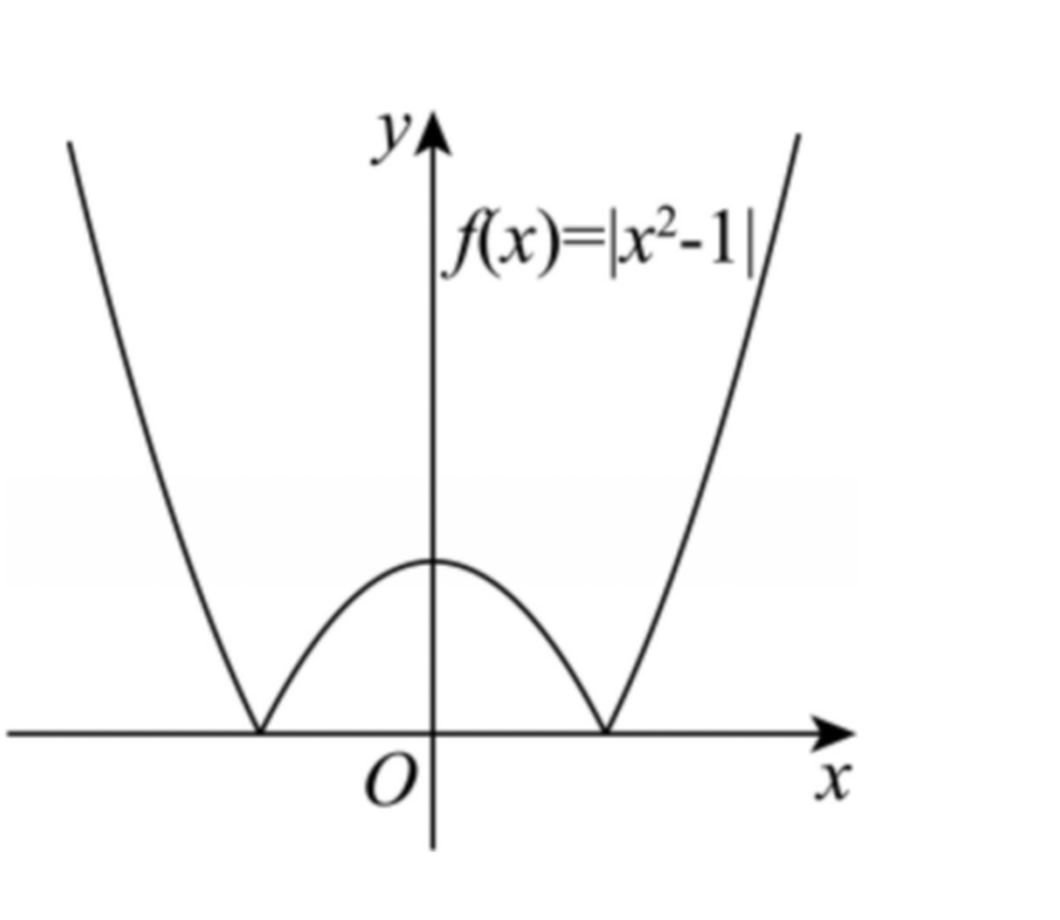
\includegraphics[width=0.40\textwidth]{figures/gao123_q20.png}
\end{center}
\step{$t=0$ 或 $t>1$ 时，每一个 $t$ 值对应 $2$ 个不同的 $x$ 值，}
\step{$t=1$ 时一个 $t$ 值对应 $3$ 个不同的 $x$ 值，}
\step{$0<t<1$ 时一个 $t$ 值对应 $4$ 个不同的 $x$ 值，}
\step{要使原方程有四个不等实根，}
\step{①$(*)$ 式一根为零，另一根大于 $1$，无解；}
\step{②$(*)$ 有两不等根且两根均大于 $1$，则 $\begin{cases}\Delta>0\\t_{\text{对}}=k>1\\f(1)>0\end{cases}$，解得 $\dfrac{1+\sqrt5}{2}<k<2$；}
\step{④$(*)$ 式有 $1$ 实根在 $(0,1)$ 之间，另一根小于零，}% 原卷由 ② 直接跳到 ④，缺 ③，照录
\step{则 $\begin{cases}f(0)<0\\f(1)>0\end{cases}$，所以 $\begin{cases}k+1<0\\2-k>0\end{cases}$，解得 $k<-1$，}
\step{综上所述，$k$ 取值范围为 $(-\infty,-1)\cup\left(\dfrac{1+\sqrt5}{2},2\right)$；}
\step{(3) 因为 $\dfrac1{a+2b}+\dfrac1{a+3}=\dfrac{a+2b+a+3}{(a+2b)(a+3)}=\dfrac{2(a+b)+3}{(a+2b)(a+3)}=\dfrac12$，}
\step{所以 $2(a+b)+3=\dfrac12(a+2b)(a+3)$，}
\step{因为 $a$、$b$ 为正实数，所以 $\dfrac12=\dfrac1{a+2b}+\dfrac1{a+3}\geqslant2\sqrt{\dfrac1{a+2b}\times\dfrac1{a+3}}$，}
\step{得 $\dfrac1{16}\geqslant\dfrac1{a+2b}\times\dfrac1{a+3}$，即 $(a+2b)(a+3)\geqslant16$，}
\step{所以 $2(a+b)+3\geqslant8$，即 $a+b\geqslant\dfrac52$，}
\step{当且仅当 $\dfrac1{a+2b}=\dfrac1{a+3}$ 即 $a=1$,$b=\dfrac32$ 时取等号，}
\step{故 $k\geqslant\dfrac52$，此时有 $\begin{cases}\Delta>0\\t_{\text{对}}=k>1\\f(0)>0,f(1)<0\end{cases}$，}
\step{故 $(*)$ 式有两不等实根且一根在 $(0,1)$ 之间，另一根大于 $1$，}
\step{故原方程有 $6$ 个实根.}
\solend
\fi

\item 设 $n$ 是不小于 $3$ 的正整数，集合 $S_n=\{(a_1,a_2,\cdots,a_n)\mid a_i\in\{0,1\},i=1,2,\cdots,n\}$，对于集合 $S_n$ 中任意两个元素 $A=(a_1,a_2,\cdots,a_n)$，$B=(b_1,b_2,\cdots,b_n)$.

定义 1：$A\cdot B=n-(\lvert a_1-b_1\rvert+\lvert a_2-b_2\rvert+\cdots+\lvert a_n-b_n\rvert)$，

定义 2：若 $A\cdot B=0$，则称互为相反元素，记作 $A=\overline B$ 或 $B=\overline A$.

(1) 若 $n=3$，$A=(0,1,0)$，$B=(1,1,0)$，试写出 $\overline A$、$\overline B$ 以及 $A\cdot B$ 的值；

(2) 若 $A$、$B\in S_n$，$A=(a_1,a_2,\cdots,a_n)$，$B=(b_1,b_2,\cdots,b_n)$，证明：$A\cdot B+\overline A\cdot B=n$；

(3) 设 $k$ 是小于 $n$ 的正奇数，至少含有两个元素的集合 $M\subseteq S_n$，且对于集合 $M$ 中任意两个不相同的元素 $A=(a_1,a_2,\cdots,a_n)$，$B=(b_1,b_2,\cdots,b_n)$，都有 $A\cdot B=n-k$，试求集合 $M$ 中元素个数的所有可能值.

\ifanswer
\solbegin
\step{(1) $\overline A=(1,0,1)$,$\overline B=(0,0,1)$,$\overline A\cdot\overline B=2$；}
\step{(2) 设 $A=(a_1,a_2,\cdots,a_n)$,$B=(b_1,b_2,\cdots,b_n)$,$\overline A=(x_1,x_2,\cdots,x_n)$，}
\step{由 $a_i$、$b_i$、$x_i\in\{0,1\}$，$i=1,2,\cdots,n$，得 $\lvert a_i-x_i\rvert\leqslant1$，$i=1,2,\cdots,n$，}
\step{所以 $\lvert a_1-x_1\rvert+\lvert a_2-x_2\rvert+\cdots+\lvert a_i-x_i\rvert\leqslant n$，}% 原卷末项下标作 $i$，照录
\step{当且仅当 $\lvert a_i-x_i\rvert=1$，$i=1,2,\cdots,n$，}
\step{即 $x_i=1-a_i$，$i=1,2,\cdots,n$ 时取等号.}
\step{由题意得 $A\cdot\overline A=n-(\lvert a_1-x_1\rvert+\lvert a_2-x_2\rvert+\cdots+\lvert a_n-x_n\rvert)=0$，}
\step{即 $\lvert a_1-x_1\rvert+\lvert a_2-x_2\rvert+\cdots+\lvert a_n-x_n\rvert=n$，}
\step{所以 $x_i=1-a_i$，$i=1,2,\cdots,n$，}
\step{$A\cdot B+\overline A\cdot B=2n-\sum\limits_{i=1}^n[\lvert a_i-b_i\rvert+(1-a_i)-b_i]$}
\step{$=2n-\sum\limits_{i=1}^n(\lvert1-b_i\rvert+\lvert0-b_i\rvert)=2n-\sum\limits_{i=1}^n(1-b_i+b_i)=2n-n=n$；}
\step{(3) 假设 $A=(a_1,a_2,\cdots,a_n)$，$B=(b_1,b_2,\cdots,b_n)$，$C=(c_1,c_2,\cdots,c_n)$}
\step{为集合 $M$ 中的三个不相同的元素，}
\step{则 $A\cdot B=n-(\lvert a_1-b_1\rvert+\lvert a_2-b_2\rvert+\cdots+\lvert a_n-b_n\rvert)=n-k$，}
\step{即 $\lvert a_1-b_1\rvert+\lvert a_2-b_2\rvert+\cdots+\lvert a_n-b_n\rvert=k$，}
\step{又由题意得 $\lvert a_i-b_i\rvert=0$ 或 $1$，$i=1,2,\cdots,n$，}
\step{$\lvert a_1-b_1\rvert$、$\lvert a_2-b_2\rvert$、$\cdots$、$\lvert a_n-b_n\rvert$ 恰有 $k$ 个 $1$，$n-k$ 个 $0$，}
\step{设其中 $k$ 个等于 $1$ 的项以此为 $a_{m_1}-b_{m_1}$,$a_{m_2}-b_{m_2}$,$\cdots$,$a_{m_k}-b_{m_k}$，}
\step{$n-k$ 个等于 $0$ 的项为 $a_{m_{k+1}}-b_{m_{k+1}}$,$a_{m_{k+2}}-b_{m_{k+2}}$,$\cdots$,$a_{m_n}-b_{m_n}$，}
\step{由题意得 $A\cdot C=n-(\lvert a_1-c_1\rvert+\lvert a_2-c_2\rvert+\cdots+\lvert a_n-c_n\rvert)=n-k$，}
\step{所以 $\sum\limits_{i=1}^k\lvert a_{m_i}-c_{m_i}\rvert+\sum\limits_{j=k+1}^n\lvert a_{m_j}-c_{m_j}\rvert=k$ ①，}
\step{同理 $\sum\limits_{i=1}^k\lvert b_{m_i}-c_{m_i}\rvert+\sum\limits_{j=k+1}^n\lvert b_{m_j}-c_{m_j}\rvert=k$ ②，}
\step{因为 $\lvert a_{m_{k+1}}-b_{m_{k+1}}\rvert=\lvert a_{m_{k+2}}-b_{m_{k+2}}\rvert=\cdots=\lvert a_{m_n}-b_{m_n}\rvert=0$，}
\step{所以 $\sum\limits_{j=k+1}^n\lvert a_{m_j}-c_{m_j}\rvert=\sum\limits_{j=k+1}^n\lvert b_{m_j}-c_{m_j}\rvert$，}
\step{由①$-$②得 $\sum\limits_{i=1}^k(\lvert a_{m_i}-c_{m_i}\rvert-\lvert b_{m_i}-c_{m_i}\rvert)=0$，}
\step{又 $\sum\limits_{i=1}^k(\lvert a_{m_i}-c_{m_i}\rvert-\lvert b_{m_i}-c_{m_i}\rvert)=\sum\limits_{i=1}^k(\lvert1-c_{m_i}\rvert-\lvert0-c_{m_i}\rvert)=k-2\sum\limits_{i=1}^k c_{m_i}$}
\step{为奇数，与 $\sum\limits_{i=1}^k(\lvert a_{m_i}-c_{m_i}\rvert-\lvert b_{m_i}-c_{m_i}\rvert)=0$ 矛盾，所以假设不成立，}
\step{即集合 $M$ 中至多有两个元素，}
\step{当 $M=\{(1,1,\cdots,1,0,0,\cdots,0),(0,0,\cdots,0)\}$ 时符合题意，}
\step{所以集合 $M$ 中元素的个数只可能是 $2$.}
\solend
\fi

\end{enumerate}

\end{document}
"
%
% 原始材料：微信公众号“魔都数学加油站”文章，作者破晓，2026-11-09 17:52 发布；
% 连载“27学年高一123”，原文标题“27学年高一123——2026-2027年上海市行知中学高一上10月月考”；
% 原文链接：https://mp.weixin.qq.com/s/GV4SWBLUJrBhMQwo22FVzg。
% 正文为 14 张 PNG 页（第 7、9、11、13、14 页 2560×3620，其余 4762×6735），
% 题目下印有【答案】或【解析】，为讲评版。
% 题目、解析均据原图转录；卷面红色水印及公众号页脚未录入。
% 全卷 3 张插图：第 5 题的坐标示意图、第 17 题的文氏图（均属题干，三版都出）、
% 第 20 题 (2) 的 $t=\lvert x^2-1\rvert$ 图象（属解析，仅答案版出）；
% 都取原卷截图去水印、2× LANCZOS 放大，见 figures/gao123_q5.png、
% figures/gao123_q17.png、figures/gao123_q20.png。
%
% 卷首标题：原卷印作“2026-2027 年行知中学高一上 10 月月考”（公众号标题中的“上海市”
% 卷面标题行没有，本稿照卷面），年份区间按全稿惯例排 en dash；原卷未印副标题，本稿按题目内容
% 标为“集合与常用逻辑用语、不等式”（与 110／111／113／116／118／120 同）。
%
% 与原卷的排版差异：
%   ① 原文从第 3 题起，填空题编号为 3—12、选择题为 13—16、解答题为 17—21，本稿保留原题号；
%   ② 原卷每题下直接印【解析】／【答案】，本稿按全稿惯例置于答案版；第 3 题只印【答案】、
%      另提 \ans{}；选择题答案在解析末句“故选 …”，括号内留空；
%   ③ 原卷未印副标题，本稿按“知识模块”口径补出；
%   ④ 原卷填空横线按全稿惯例排为 \blankline[4.4em]；选择题括号排 \mbox{（\quad）}、
%      选项段前按惯例加 \keepwithprev；解答题不留作答区（原卷为讲评版，与 109—122 同）；
%   ⑤ 原卷数集排斜体 $R$／$Z$（第 9 题作粗体 $\mathbf{R}$），按全稿惯例改 \R／\Z；
%      绝对值按全稿惯例排 \lvert…\rvert，集合描述竖线排 \mid；单位 km、h 原卷排斜体，
%      本稿按正体照排；补集照原卷上划线排 \overline{B}、\overline{A}。
%
% 判别式与子集符号：第 16 题解析的 $\triangle=b^2-4c<0$、第 20 题 (1) ① 的 $\triangle<0$
%   均作等边、扁的 \triangle；第 20 题 ② 两处 cases 与 (3) 的 $\Delta\geqslant0$／$\Delta>0$
%   作等腰、高的 \Delta，逐处照录、不统一；第 15 题选项与第 17 题 (2) 的 $\subseteq$
%   印有下划线，照录 \subseteq。
%
% 原卷存疑照录：
%   第 4 题解析“若 $-\lvert a\rvert=0$，则 $a=0$，则 $A=\{0,-1,0\}$”以元素重复说明互异性；
%   第 5 题解析“当 $a^2+b^2=400^2+b^2<500^2$”等式左边 $a^2$ 与 $400^2$ 并用；
%   第 9 题解析“解得 $a>1$ 得 $a<\dfrac13$”（按平方不等式应为 $a>1$ 或 $a<\dfrac13$）；
%   第 12 题解析“所以 $-\dfrac1{2^a}\cdot\dfrac1{2^b}\geqslant-\dfrac14$”带负号起论；
%   第 17 题 (1) 解析把阴影部分（实为 $A\cap\overline B$）印作 $\overline{A\cap B}$；
%   第 18 题 (2) 解析作“$n<1$，所以 $n-1<0$”，与题设 $m<1$ 字母不一致；
%   第 20 题 (2) 的情形编号由 ①、② 直接跳到 ④（缺 ③）；
%   第 21 题 (2) 解析“$\lvert a_1-x_1\rvert+\cdots+\lvert a_i-x_i\rvert\leqslant n$”
%   末项下标作 $i$（按上下文应为 $n$）。以上均照录加注。
%
% 行数核对：逐题数 \step 条数，合计 176 条（Q3：0；Q4：6；Q5：5；Q6：5；Q7：4；
% Q8：6；Q9：5；Q10：5；Q11：10；Q12：6；Q13：9；Q14：1；Q15：5；Q16：21；
% Q17：8；Q18：14；Q19：10；Q20：26；Q21：30），与原卷印刷行逐题相等
% （cases 块作一个印刷行计）。第 3 题只印【答案】，提 \ans{}，不计入 \step 账。
%
\documentclass[a4paper,11pt]{article}
\usepackage{common}

\begin{document}

\examtitlest[3]{2026--2027 年行知中学高一上 10 月月考}{集合与常用逻辑用语、不等式}

\bigsec{一、填空题}

\begin{enumerate}
\setcounter{enumi}{2}

\item 写出命题“存在实数 $x$、$y$、$z$，使 $x<y$ 或 $y<z$.”的否定\blankline[4.4em].

\ifanswer
\ans{任意实数 $x$、$y$、$z$，使得 $x\geqslant y$ 且 $y\geqslant z$}
\fi

\item 若集合 $\{0,-1,2a\}=\{a-1,-\lvert a\rvert,a+1\}$，实数 $a$ 的值为\blankline[4.4em].

\ifanswer
\solbegin
\step{令 $A=\{0,-1,2a\}$,$B=\{a-1,-\lvert a\rvert,a+1\}$，}
\step{因为 $\{0,-1,2a\}=\{a-1,-\lvert a\rvert,a+1\}$，}
\step{若 $a-1=0$，则 $a=1$，则 $A=\{0,-1,2\}$,$B=\{0,-1,2\}$，满足要求；}
\step{若 $-\lvert a\rvert=0$，则 $a=0$，则 $A=\{0,-1,0\}$，不满足集合元素的互异性；}% 原卷以 $A=\{0,-1,0\}$ 说明互异性，照录
\step{若 $a+1=0$，则 $a=-1$，则 $A=\{0,-1,-2\}$,$B=\{0,-1,-2\}$，满足要求；}
\step{故实数 $a$ 的值为 $\pm1$.}
\solend
\fi

\needvspace{7cm}
\item 如图，据气象部门预报，在距离某码头南偏东 $45^\circ$ 方向 $400\sqrt2$ km 处的热带
风暴中心正在以 $20$km/h 的速度向正北方向移动，距风暴中心 $500$km 以内
的地区都将受到影响. 以上预报估计，该码头将受到热带风暴的影响时长大
约为\blankline[4.4em]$h$.

\begin{center}
% 图取原卷截图（第 1 页题干右侧）、去水印后 2× LANCZOS 放大，本稿移至题干之后
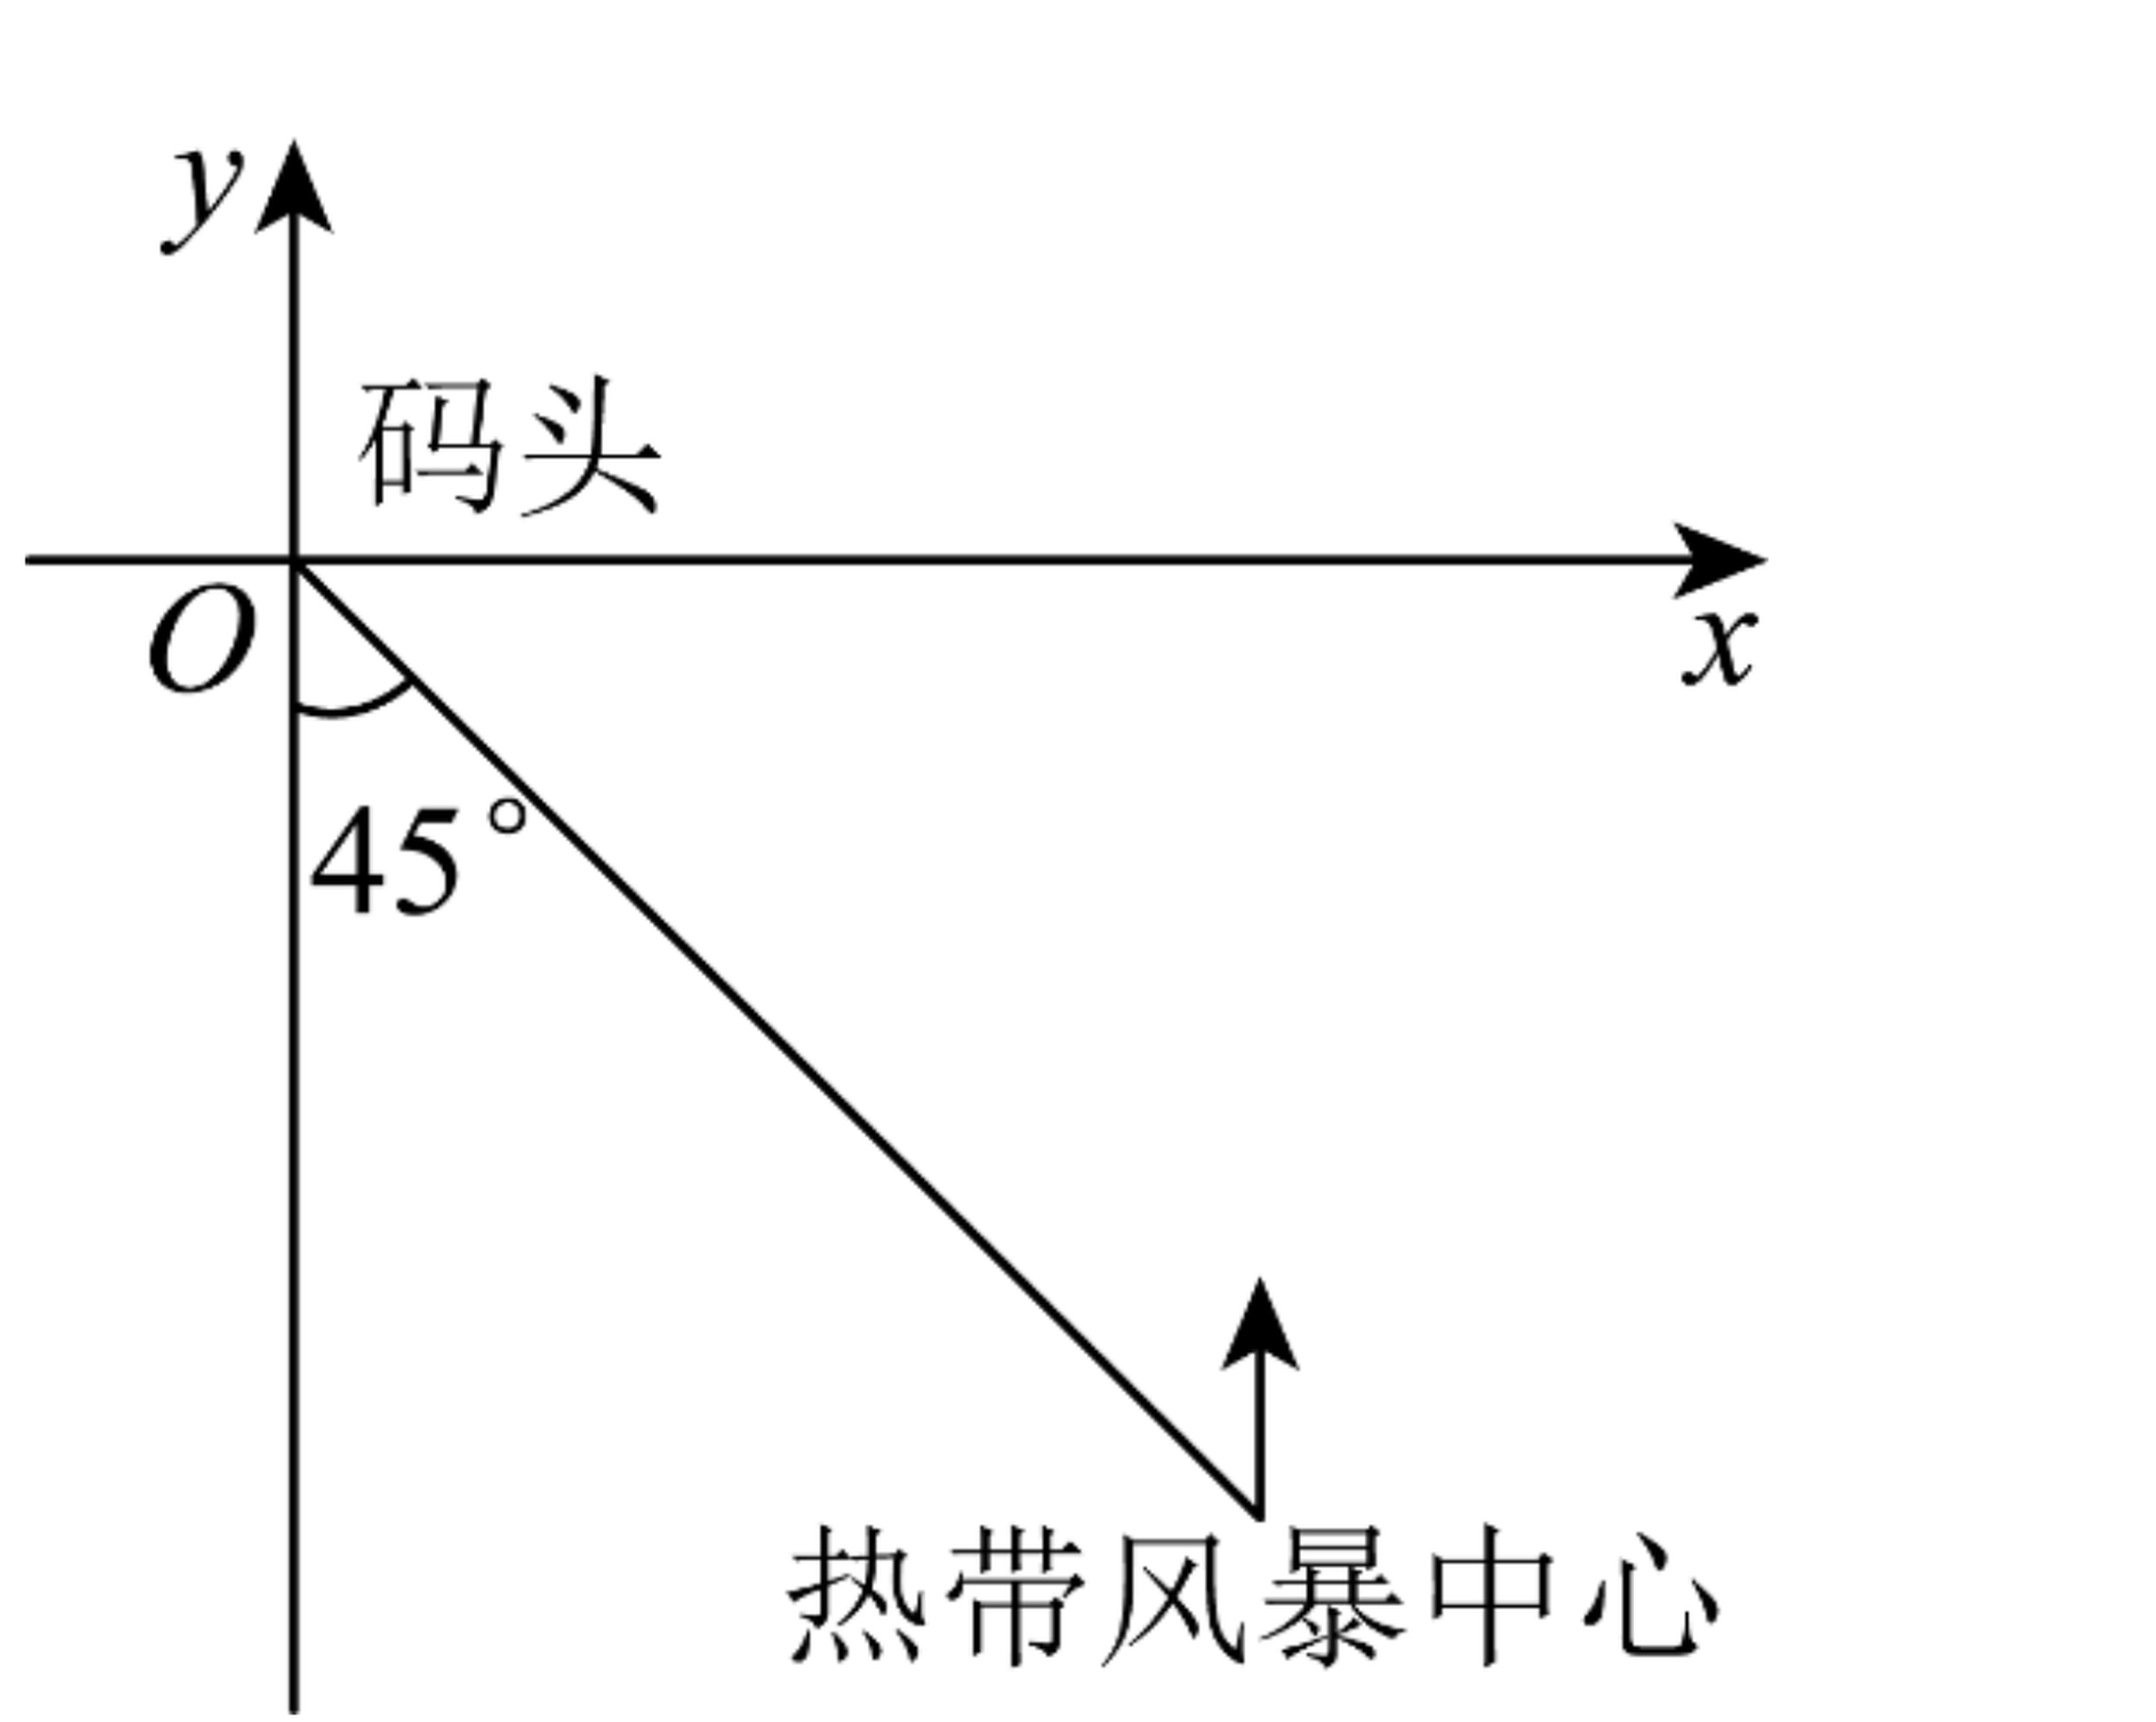
\includegraphics[width=0.36\textwidth]{figures/gao123_q5.png}
\end{center}

\ifanswer
\solbegin
\step{设风暴中心的坐标为 $(a,b)$，}
\step{由题意得 $a=400\sqrt2\times\cos45^\circ=400$，当 $a^2+b^2=400^2+b^2<500^2$，}% 原卷 $a^2$ 与 $400^2$ 并用，照录
\step{即 $-300<b<300$ 时，码头将受到风暴影响，}
\step{$\dfrac{300-(-300)}{20}=30h$，则码头受到风暴影响的时长为 30 小时，}
\step{所以由预报估计，该码头将受到热带风暴的影响时长大约为 30 小时.}
\solend
\fi

\item 已知 $a$、$b$、$c$ 为常数，若不等式 $\dfrac{ax-b}{x-c}\geqslant0$ 的解集为 $[-1,1)$，则不等式 $ax+b<0$ 的解集为\blankline[4.4em].

\ifanswer
\solbegin
\step{不等式 $\dfrac{ax-b}{x-c}\geqslant0$ 可化为 $(ax-b)(x-c)\geqslant0$ 且 $x-c\neq0$，}
\step{即 $a\left(x-\dfrac ba\right)(x-c)\geqslant0$ 且 $x\neq c$，}
\step{因为不等式 $\dfrac{ax-b}{x-c}\geqslant0$ 的解集为 $[-1,1)$，所以 $a<0$，且 $\dfrac ba=-1$,$c=1$，}
\step{即 $b=-a$，所以不等式 $ax+b<0$ 可化为 $ax-a<0$，又因为 $a<0$，所以 $x-1>0$，}
\step{解得 $x>1$，所以不等式 $ax+b<0$ 的解集为 $(1,+\infty)$.}
\solend
\fi

\item 已知实数 $a$、$b$ 满足 $ab=32$，且 $\log_2a=\log_b16$，则 $a+b$ 的值为\blankline[4.4em].

\ifanswer
\solbegin
\step{由 $\log_2a=\log_b16$，得 $\log_2a=\dfrac{\log_216}{\log_2b}$，则 $\log_2a\cdot\log_2b=4$，}
\step{由 $ab=32$，得 $\log_2a+\log_2b=\log_2ab=5$，}
\step{得 $\log_2a=1$,$\log_2b=4$ 或 $\log_2a=4$,$\log_2b=1$，}
\step{因此 $a=2$,$b=16$ 或 $a=16$,$b=2$，所以 $a+b=18$.}
\solend
\fi

\item 已知实数 $a$、$b$ 满足 $-3<a+2b<2$，$-1<2a-b<4$，则 $a+b$ 的取值范围为\blankline[4.4em].

\ifanswer
\solbegin
\step{设 $a+b=m(a+2b)+n(2a-b)=(m+2n)a+(2m-n)b$，}
\step{所以 $\begin{cases}m+2n=1\\2m-n=1\end{cases}$，解得 $n=\dfrac15$,$m=\dfrac35$，所以 $a+b=\dfrac35(a+2b)+\dfrac15(2a-b)$，}
\step{因为 $-3<(a+2b)<2$，$-1<2a-b<4$，}
\step{所以 $-\dfrac95<\dfrac35(a+2b)<\dfrac65$，$-\dfrac15<\dfrac15(2a-b)<\dfrac45$，}
\step{相加得 $-2<\dfrac35(a+2b)+\dfrac15(2a-b)<2$，即 $-2<a+b<2$，}
\step{故 $a+b$ 的取值范围为 $(-2,2)$.}
\solend
\fi

\item 存在 $x\in\R$ 使不等式 $\lvert2x-a\rvert<\lvert2a-1\rvert-2\lvert x\rvert$ 成立，则实数 $a$ 的取值范围是\blankline[4.4em].

\ifanswer
\solbegin
\step{存在 $x\in\R$，不等式 $\lvert2x-a\rvert<\lvert2a-1\rvert-2\lvert x\rvert$ 成立，}
\step{变形即 $\lvert2x-a\rvert+2\lvert x\rvert<\lvert2a-1\rvert$ 成立，}
\step{由于 $\lvert2x-a\rvert+\lvert2x\rvert\geqslant\lvert(2x-a)-2x\rvert=\lvert a\rvert$，当且仅当 $2x(2x-a)\leqslant0$ 时取等号，}
\step{因此有 $\lvert a\rvert<\lvert2a-1\rvert$，两边平方 $a^2<(2a-1)^2$，解得 $a>1$ 得 $a<\dfrac13$，}% 原卷“解得 a>1 得 a<1/3”，照录
\step{即实数 $a$ 的取值范围是 $\left(-\infty,\dfrac13\right)\cup(1,+\infty)$.}
\solend
\fi

\item 已知集合 $A=\{(x,y)\mid x^2+mx-y+2=0\}$，$B=\{(x,y)\mid x-y+1=0,0\leqslant x\leqslant3\}$，若集合 $A\cap B$ 的子集个数为 $2$，则实数 $m$ 的取值范围为\blankline[4.4em].

\ifanswer
\solbegin
\step{因为集合 $A\cap B$ 的子集个数为 $2$，所以 $A\cap B$ 的元素有一个，}
\step{即 $\begin{cases}x^2+mx-y+2=0\\x-y+1=0\end{cases}$ 在 $x\in[0,3]$ 上只有一个解，}
\step{即 $x^2+(m-1)x+1=0$ 在 $[0,3]$ 上只有一个解，}
\step{即 $1-m=x+\dfrac1x$ 在 $[0,3]$ 上只有一个解，}
\step{结合对勾函数的性质得 $1-m=2$ 或 $1-m>\dfrac{10}{3}$，解得 $m=-1$ 或 $m<-\dfrac73$.}
\solend
\fi

\item $[x]$ 表示不超过 $x$ 的最大整数，则集合 $A=\left\{y\,\middle\vert\,y=\left[\dfrac{x^2}{100}\right],x=1,2,3,\cdots,100\right\}$ 中的元素个数为\blankline[4.4em].

\ifanswer
\solbegin
\step{记 $a_k=\left[\dfrac{k^2}{100}\right](k=1,2,\cdots,100)$，$a_k$ 随 $k$ 增大而单调不减.}
\step{当 $k\geqslant50$ 时，$\dfrac{(k+1)^2}{100}-\dfrac{k^2}{100}=\dfrac{2k+1}{100}\geqslant\dfrac{101}{100}>1$，所以 $a_{k+1}\geqslant a_k+1$，}
\step{即 $a_{50}$、$a_{51}$、$\cdots$、$a_{100}$ 两两互异.}
\step{又 $a_{50}=\left[\dfrac{2500}{100}\right]=25$、$a_{100}=100$，这一段共 $100-50+1=51$ 个互异的值，}
\step{且都大于等于 $25$.}
\step{当 $k\leqslant49$ 时，$\dfrac{(k+1)^2}{100}-\dfrac{k^2}{100}=\dfrac{2k+1}{100}\leqslant\dfrac{99}{100}<1$，即 $a_k$ 每次至多增加 $1$；}
\step{又 $a_1=0$、$a_{49}=\left[\dfrac{2401}{100}\right]=24$，}
\step{故 $a_1$、$a_2$、$\cdots$、$a_{49}$ 依次取遍 $0$，$1$，$2$，$\cdots$，$24$，共 $25$ 个值.}
\step{两段取值范围互不重叠（前段不超过 $24$、后段不小于 $25$），}
\step{所以集合 $A$ 中共有 $25+51=76$ 个元素.}
\solend
\fi

\item 若实数 $a$、$b$、$c$ 满足 $\dfrac1{2^a}+\dfrac1{2^b}=1$，$\dfrac1{2^{a+b}}+\dfrac1{2^{b+c}}+\dfrac1{2^{a+c}}=1$，则 $c$ 的最大值是\blankline[4.4em].

\ifanswer
\solbegin
\step{因为 $\dfrac1{2^a}+\dfrac1{2^b}=1$，}
\step{由基本不等式得 $1=\dfrac1{2^a}+\dfrac1{2^b}\geqslant2\sqrt{\dfrac1{2^a}\cdot\dfrac1{2^b}}$（当且仅当 $a=b=1$ 时取等号），}
\step{所以 $\dfrac1{2^a}\cdot\dfrac1{2^b}\leqslant\dfrac14$，所以 $-\dfrac1{2^a}\cdot\dfrac1{2^b}\geqslant-\dfrac14$，}% 原卷带负号起论，照录
\step{因为 $\dfrac1{2^{a+b}}+\dfrac1{2^{b+c}}+\dfrac1{2^{a+c}}=1$，$\dfrac1{2^{b+c}}+\dfrac1{2^{a+c}}=\dfrac1{2^c}\left(\dfrac1{2^a}+\dfrac1{2^b}\right)=\dfrac1{2^c}$，}
\step{所以 $\dfrac1{2^c}=1-\dfrac1{2^{a+b}}\geqslant\dfrac34$，所以 $2^c\leqslant\dfrac43$，所以 $c\leqslant\log_2\dfrac43=2-\log_23$，}
\step{故 $c$ 的最大值是 $2-\log_23$.}
\solend
\fi

\end{enumerate}

\bigsec{二、选择题}

\begin{enumerate}
\setcounter{enumi}{12}

\item 下列运用等式或不等式的性质变形中，正确的是\mbox{（\quad）}

\keepwithprev
A. 如果 $a=b$，那么 $\dfrac ac=\dfrac bc$\qquad\qquad B. 如果 $\dfrac1a<\dfrac1b<0$，那么 $a-\dfrac1a>b-\dfrac1b$

C. 如果 $a>b$，那么 $\dfrac1a<\dfrac1b$\qquad\qquad D. 如果 $a>b>0$，$m\in\R$，那么 $\dfrac ba<\dfrac{b+m}{a+m}$

\ifanswer
\solbegin
\step{对于 $A$，若 $c=0$，$A$ 错误；}
\step{对于 $B$，若 $\dfrac1a<\dfrac1b<0$，则 $0>a>b$，$-\dfrac1a>-\dfrac1b>0$，}
\step{所以 $a-\dfrac1a>b-\dfrac1b$，$B$ 正确；}
\step{对于 $C$，$a>0$，$b<0$ 时，$C$ 错误；}
\step{对于 $D$，$\dfrac{b+m}{a+m}-\dfrac ba=\dfrac{ab+am}{a(a+m)}-\dfrac{ab+bm}{a(a+m)}=\dfrac{(a-b)m}{a(a+m)}$，}
\step{因为 $a>b>0$，所以 $a-b>0$，但 $m$、$a+m$ 的符号不确定，}
\step{当 $m=0$ 时，$\dfrac ba=\dfrac{b+m}{a+m}$，}
\step{当 $m(a+m)>0$ 时，$\dfrac ba<\dfrac{b+m}{a+m}$，当 $m(a+m)<0$ 时，$\dfrac ba>\dfrac{b+m}{a+m}$，$D$ 错误.}
\step{故选 $B$.}
\solend
\fi

\item “$a>b$”的一个必要非充分条件是\mbox{（\quad）}

\keepwithprev
A. $ac^2>bc^2$\qquad\quad B. $2^a>2^b$\qquad\quad C. $\left(\dfrac12\right)^{a-b}\leqslant1$\qquad\quad D. $a^3>b^3$

\ifanswer
\solbegin
\step{即“$a>b$”能推出选项，但选项不能推出“$a>b$”，故选 $C$.}
\solend
\fi

\item 若 $A=\left\{x\,\middle\vert\,x=\dfrac k6+1,k\in\Z\right\}$，$B=\left\{x\,\middle\vert\,x=\dfrac k3+\dfrac12,k\in\Z\right\}$，$C=\left\{x\,\middle\vert\,x=\dfrac{2k}{3}+\dfrac12,k\in\Z\right\}$，则这三个集合间的关系是\mbox{（\quad）}

\keepwithprev
A. $A\subseteq B\subseteq C$\qquad\quad B. $A\subseteq C\subseteq B$\qquad\quad C. $C\subseteq B\subseteq A$\qquad\quad D. $C\subseteq A\subseteq B$

\ifanswer
\solbegin
\step{若 $x\in C$，则存在 $k_0\in\Z$，使 $x=\dfrac{2k_0}{3}+\dfrac12$，}
\step{又 $2k_0\in\Z$，所以 $x\in B$，故 $C\subseteq B$，}
\step{若 $x\in B$，则存在 $k_1\in\Z$，使 $x=\dfrac{k_1}{3}+\dfrac12=\dfrac{2k_1-3}{6}+1$，}
\step{又 $2k_1-3\in\Z$，所以 $x\in A$，故 $B\subseteq A$，}
\step{又 $\dfrac43\in A$，$\dfrac43\notin B$，$\dfrac56\in B$，$\dfrac56\notin C$，所以 $C\subseteq B\subseteq A$，故选 $C$.}
\solend
\fi

\item 集合 $S=\{x\mid(x+a)(x^2+bx+c)=0\}$，$T=\{x\mid(ax+1)(cx^2+bx+1)=0\}$，其中 $a$、$b$、$c$ 为实数，若 $\lvert S\rvert$、$\lvert T\rvert$ 分别表示 $S$、$T$ 的元素个数，则下列结论中一定成立的是\mbox{（\quad）}

\keepwithprev
A. 若 $\lvert T\rvert=0$，则 $\lvert S\rvert=1$\qquad\qquad B. 若 $\lvert S\rvert=1$，则 $\lvert T\rvert=1$

C. 若 $\lvert S\rvert=2$，则 $\lvert T\rvert=2$\qquad\qquad D. 若 $\lvert T\rvert=3$，则 $\lvert S\rvert=2$

\ifanswer
\solbegin
\step{令 $f(x)=(x+a)(x^2+bx+c)$,$g(x)=(ax+1)(cx^2+bx+1)$，}
\step{对于选项 A，当 $\lvert T\rvert=0$ 时，方程 $g(x)=(ax+1)(cx^2+bx+1)=0$ 无实根，}
\step{当 $a=b=c=0$ 时，$f(x)=x^3$，由 $f(x)=0$ 得 $x=0$，此时 $\lvert S\rvert=1$；}
\step{当 $a=0$,$b^2-4c<0$ 时，$f(x)=x(x^2+bx+c)$，由 $f(x)=0$ 得 $x=0$，}
\step{此时 $\lvert S\rvert=1$，所以选项 A 正确；}
\step{对于选项 B，若 $\lvert S\rvert=1$，则 $f(x)=(x+a)(x^2+bx+c)=0$ 有且只有一根，}
\step{又 $x=-a$ 一定是 $f(x)=0$ 的根，所以 $\triangle=b^2-4c<0$，}
\step{又 $\triangle=b^2-4c<0$ 且 $a=0$ 时，$g(x)=(ax+1)(cx^2+bx+1)=0$ 无解，}
\step{此时 $\lvert T\rvert=0$，所以选项 B 错误，}
\step{对于选项 C，若 $\lvert S\rvert=2$ 时，则 $f(x)=(x+a)(x^2+bx+c)=0$ 有且只有 $2$ 根，}
\step{又 $x=-a$ 一定是 $f(x)=0$ 的根，}
\step{所以 $\triangle=b^2-4c=0$ 且 $a^2+ab+c\neq0$ 或 $\triangle=b^2-4c>0$ 且 $a^2+ab+c=0$，}
\step{当 $a=0$ 时，存在 $b$,$c$，使 $\triangle=b^2-4c=0$ 且 $a^2+ab+c\neq0$，}
\step{此时 $g(x)=(ax+1)(cx^2+bx+1)=0$ 只有一根，所以选项 C 错误，}
\step{对于选项 D，当 $\lvert T\rvert=3$ 时，方程 $g(x)=(ax+1)(cx^2+bx+1)=0$ 有三个根，}
\step{所以 $a\neq0$,$c\neq0$,$b^2-4c>0$，}
\step{设 $x_0$ 为 $g(x)=0$ 的一个根，即 $(ax_0+1)(cx_0^2+bx_0+1)=0$，}
\step{则 $x_0\neq0$，且 $f\left(\dfrac1{x_0}\right)=\left(\dfrac1{x_0}+a\right)\left(\dfrac1{x_0^2}+\dfrac1{x_0}b+c\right)=\dfrac1{x_0^3}g(x_0)=0$，}
\step{所以 $\dfrac1{x_0}$ 为方程 $f(x)=0$ 的根，故 $f(x)=0$ 有三个根，即 $\lvert T\rvert=3$ 时，}
\step{必有 $\lvert S\rvert=3$，所以选项 D 错误，}
\step{故选 $A$.}
\solend
\fi

\end{enumerate}

% 第 17 题是解答题第一题且带文氏图，守卫放在 \bigsec 之前，连节标题一起量页高
\needvspace{7cm}
\bigsec{三、解答题}

\begin{enumerate}
\setcounter{enumi}{16}

\item 设全集 $U=\R$，集合 $A=\{x\mid-2\leqslant x\leqslant4\}$，$B=\{x\mid x<-6$ 或 $x\geqslant2\}$.

（1）求图中阴影部分表示的集合；

（2）已知集合 $C=\{x\mid10-a<x<2a+1\}$，若 $\overline B\cap C=\varnothing$，求 $a$ 的取值范围.

\begin{center}
% 图取原卷截图（第 7 页题干右侧）、去水印后 2× LANCZOS 放大，本稿移至题干之后
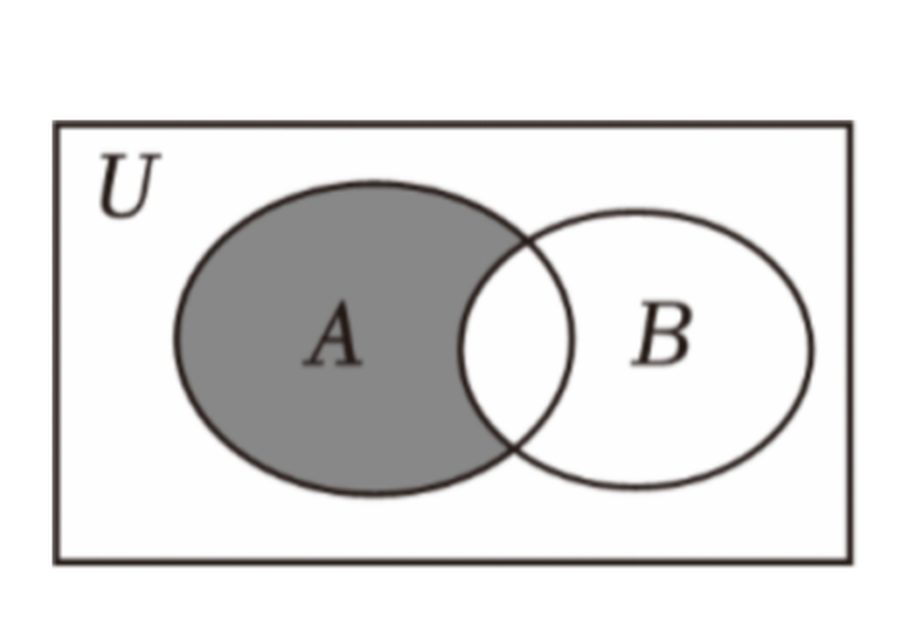
\includegraphics[width=0.34\textwidth]{figures/gao123_q17.png}
\end{center}

\ifanswer
\solbegin
\step{（1）$A\cap B=\{x\mid2\leqslant x\leqslant4\}$，}
\step{则图中阴影部分表示 $\overline{A\cap B}=\{x\mid-2\leqslant x<2\}$.}% 原卷把上划线盖在整个 $A\cap B$ 上，照录
\step{（2）由题意得 $\overline B=\{x\mid-6\leqslant x<2\}$，$C\subseteq B$，}
\step{所以当 $C=\varnothing$ 时，$10-a\geqslant2a+1$，解得 $a\leqslant3$，符合题意；}
\step{当 $C\neq\varnothing$ 时，$\begin{cases}10-a<2a+1\\2a+1\leqslant-6\end{cases}$ 或者 $\begin{cases}10-a<2a+1\\10-a\geqslant2\end{cases}$，}
\step{此时不等式组 $\begin{cases}10-a<2a+1\\2a+1\leqslant-6\end{cases}$ 无解，}
\step{不等式组 $\begin{cases}10-a<2a+1\\10-a\geqslant2\end{cases}$ 的解集为 $3<a\leqslant8$，}
\step{综上，$a$ 的取值范围为 $\{a\mid a\leqslant8\}$.}
\solend
\fi

\item (1) 求不等式：$\lvert x-1\rvert+\lvert x-2\rvert\leqslant5$ 的解集.

(2) 当 $m<1$ 时，解关于 $x$ 的不等式 $\dfrac{m(x-3)}{x+2}>1$.

\ifanswer
\solbegin
\step{(1) 当 $x<1$ 时，$\lvert x-1\rvert+\lvert x-2\rvert\leqslant5\Leftrightarrow-x+1+2-x\leqslant5$，}
\step{解得 $-1\leqslant x<1$；}
\step{当 $1\leqslant x\leqslant2$ 时，$\lvert x-1\rvert+\lvert x-2\rvert\leqslant5\Leftrightarrow x-1+2-x=1\leqslant5$ 恒成立，}
\step{所以 $1\leqslant x\leqslant2$；}
\step{当 $x>2$ 时，$\lvert x-1\rvert+\lvert x-2\rvert\leqslant5\Leftrightarrow x-1+x-2=2x-3\leqslant5$，}
\step{解得 $2<x\leqslant4$.}
\step{综上所述，不等式 $\lvert x-1\rvert+\lvert x-2\rvert\leqslant5$ 的解集为 $[-1,4]$.}
\step{(2) 原不等式变成 $\dfrac{(m-1)x-(3m+2)}{x+2}>0$，$n<1$，所以 $n-1<0$，}% 原卷作 $n<1$、$n-1<0$，与题设 $m<1$ 字母不一致，照录
\step{所以原不等式变成 $\dfrac{x-\dfrac{3m+2}{m-1}}{x+2}<0$，$\dfrac{3m+2}{m-1}-(-2)=\dfrac{5m}{m-1}$，}
\step{所以 $m<0$ 时，$\dfrac{5m}{m-1}>0$，$\dfrac{3m+2}{m-1}>-2$，}
\step{原不等式的解集为 $\left(-2,\dfrac{3m+2}{m-1}\right)$；}
\step{$m=0$ 时，原不等式变成 $1<0$，无解；}
\step{$0<m<1$ 时，$\dfrac{5m}{m-1}<0$，$\dfrac{3m+2}{m-1}<-2$，}
\step{原不等式的解集为 $\left(\dfrac{3m+2}{m-1},-2\right)$.}
\solend
\fi

\item 在园林博览会上，某公司带来了一种智能设备供采购商洽谈采购，并决定大量投放市场，已知该种设备年固定研发成本为 $50$ 万元，每生产一台需另投入 $100$ 元，设该公司一年内生产该设备 $x$ 万台且全部售完，每万台的销售收入 $G(x)$（万元）与年产量 $x$（万台）满足如下关系式：$G(x)=\begin{cases}180-x,0<x\leqslant20\\80+\dfrac{2000}{x}-\dfrac{8000}{x(x-1)},x>20\end{cases}$.

(1) 写出年利润 $W(x)$（万元）关于年产量 $x$（万台）的函数解析式；（利润 $=$ 销售收入 $-$ 成本）

(2) 当年产量为多少万台时，该公司获得的年利润最大，并求出最大利润.

\ifanswer
\solbegin
\step{(1) $W(x)=xG(x)-50-100x=\begin{cases}-50+80x-x^2,0<x\leqslant20\\-20x+1950-\dfrac{8000}{x-1},x>20\end{cases}$；}
\step{(2) 当 $0<x\leqslant20$ 时，$W(x)=-50+80x-x^2=-(x-40)^2+1550$，}
\step{由函数性质得当 $x\leqslant40$ 时严格增，所以当 $x=20$ 时，$W(x)_{max}=1150$，}
\step{当 $x>20$ 时，$W(x)=-20x+1950-\dfrac{8000}{x-1}=-20\left[(x-1)+\dfrac{400}{x-1}\right]+1930$，}
\step{$W(x)=-20\left[(x-1)+\dfrac{400}{x-1}\right]+1930\leqslant-20\times2\sqrt{(x-1)\cdot\dfrac{400}{x-1}}+1930$}
\step{$=1130$，当且仅当 $x-1=\dfrac{400}{x-1}$，即 $x=21$ 时取等号，}
\step{所以 $W(x)_{max}=1130$，}
\step{因为 $1150>1130$，所以当 $x=20$ 时，$W(x)_{max}=1150$，}
\step{即当年产量为 $20$ 万台时，该公司获得的年利润最大，}
\step{最大利润为 $1150$ 万元.}
\solend
\fi

\item 关于 $x$ 的方程 $(x^2-1)^2-2k\lvert x^2-1\rvert+k+1=0(k\in\R)$.

(1) 若方程无实根，求 $k$ 的取值范围；

(2) 若方程有 $4$ 个不等实根，求 $k$ 的取值范围；

(3) 若 $k=a+b$，且满足 $\dfrac1{a+2b}+\dfrac1{a+3}=\dfrac12$，$a>0$，$b>0$，试判断方程根的个数.

\ifanswer
\solbegin
\step{(1) 关于 $x$ 的方程 $(x^2-1)^2-2k\lvert x^2-1\rvert+k+1=0(k\in\R)$，}
\step{令 $t=\lvert x^2-1\rvert$，则 $t\geqslant0$，则原方程转化为 $t^2-2kt+k+1=0(*)$，}
\step{因为关于 $x$ 的方程 $(x^2-1)^2-2k\lvert x^2-1\rvert+k+1=0(k\in\R)$ 无实根，}
\step{所以 $(*)$ 式无实根或实根均小于零，令 $f(t)=t^2-2kt+k+1$，}
\step{①若 $(*)$ 式无实根，则 $\triangle<0$，解得 $\dfrac{1-\sqrt5}{2}<k<\dfrac{1+\sqrt5}{2}$，}
\step{②两根均为负，则 $\begin{cases}\Delta\geqslant0\\t_{\text{对}}=k<0\\f(0)>0\end{cases}$，解得 $-1<k\leqslant\dfrac{1-\sqrt5}{2}$，}
\step{综合①②，得 $k$ 的取值范围是 $\left(-1,\dfrac{1+\sqrt5}{2}\right)$；}
\step{(2) 作函数 $t=\lvert x^2-1\rvert$ 的图象，}
\begin{center}
% 图取原卷截图（第 11 页解析内）、去水印后 2× LANCZOS 放大，仅答案版出
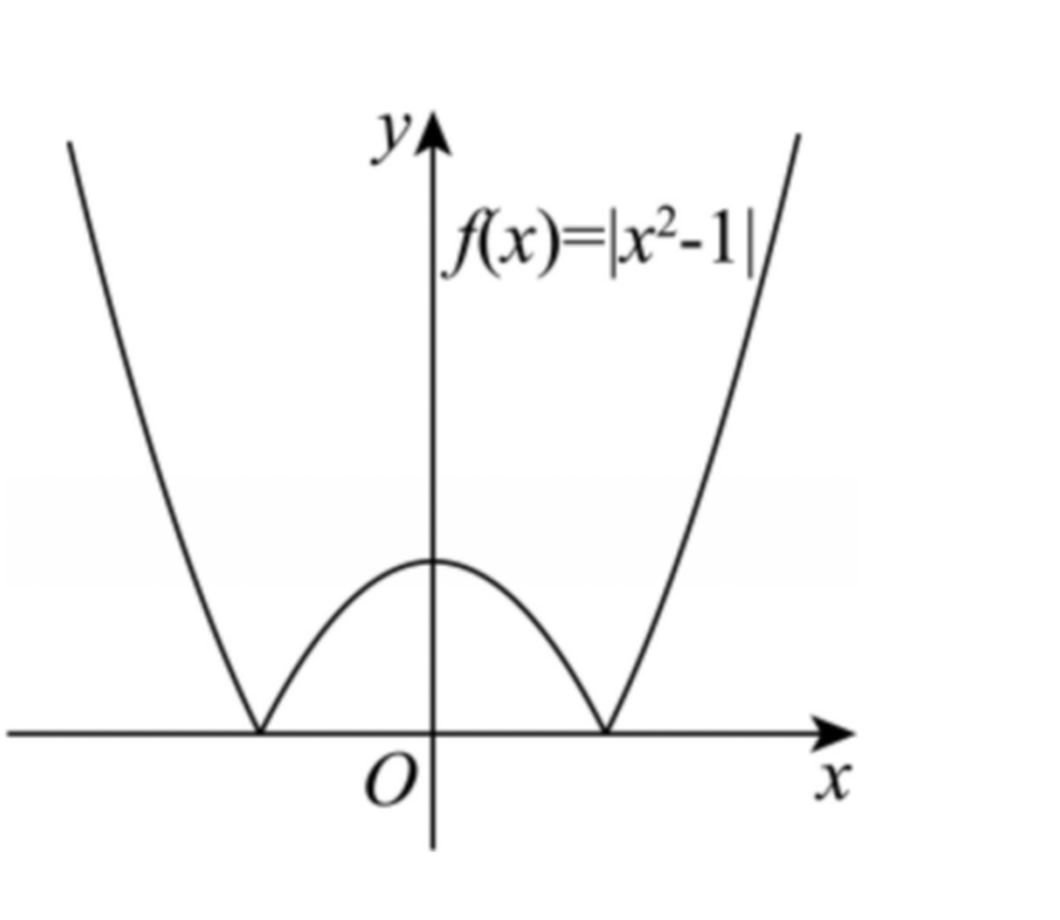
\includegraphics[width=0.40\textwidth]{figures/gao123_q20.png}
\end{center}
\step{$t=0$ 或 $t>1$ 时，每一个 $t$ 值对应 $2$ 个不同的 $x$ 值，}
\step{$t=1$ 时一个 $t$ 值对应 $3$ 个不同的 $x$ 值，}
\step{$0<t<1$ 时一个 $t$ 值对应 $4$ 个不同的 $x$ 值，}
\step{要使原方程有四个不等实根，}
\step{①$(*)$ 式一根为零，另一根大于 $1$，无解；}
\step{②$(*)$ 有两不等根且两根均大于 $1$，则 $\begin{cases}\Delta>0\\t_{\text{对}}=k>1\\f(1)>0\end{cases}$，解得 $\dfrac{1+\sqrt5}{2}<k<2$；}
\step{④$(*)$ 式有 $1$ 实根在 $(0,1)$ 之间，另一根小于零，}% 原卷由 ② 直接跳到 ④，缺 ③，照录
\step{则 $\begin{cases}f(0)<0\\f(1)>0\end{cases}$，所以 $\begin{cases}k+1<0\\2-k>0\end{cases}$，解得 $k<-1$，}
\step{综上所述，$k$ 取值范围为 $(-\infty,-1)\cup\left(\dfrac{1+\sqrt5}{2},2\right)$；}
\step{(3) 因为 $\dfrac1{a+2b}+\dfrac1{a+3}=\dfrac{a+2b+a+3}{(a+2b)(a+3)}=\dfrac{2(a+b)+3}{(a+2b)(a+3)}=\dfrac12$，}
\step{所以 $2(a+b)+3=\dfrac12(a+2b)(a+3)$，}
\step{因为 $a$、$b$ 为正实数，所以 $\dfrac12=\dfrac1{a+2b}+\dfrac1{a+3}\geqslant2\sqrt{\dfrac1{a+2b}\times\dfrac1{a+3}}$，}
\step{得 $\dfrac1{16}\geqslant\dfrac1{a+2b}\times\dfrac1{a+3}$，即 $(a+2b)(a+3)\geqslant16$，}
\step{所以 $2(a+b)+3\geqslant8$，即 $a+b\geqslant\dfrac52$，}
\step{当且仅当 $\dfrac1{a+2b}=\dfrac1{a+3}$ 即 $a=1$,$b=\dfrac32$ 时取等号，}
\step{故 $k\geqslant\dfrac52$，此时有 $\begin{cases}\Delta>0\\t_{\text{对}}=k>1\\f(0)>0,f(1)<0\end{cases}$，}
\step{故 $(*)$ 式有两不等实根且一根在 $(0,1)$ 之间，另一根大于 $1$，}
\step{故原方程有 $6$ 个实根.}
\solend
\fi

\item 设 $n$ 是不小于 $3$ 的正整数，集合 $S_n=\{(a_1,a_2,\cdots,a_n)\mid a_i\in\{0,1\},i=1,2,\cdots,n\}$，对于集合 $S_n$ 中任意两个元素 $A=(a_1,a_2,\cdots,a_n)$，$B=(b_1,b_2,\cdots,b_n)$.

定义 1：$A\cdot B=n-(\lvert a_1-b_1\rvert+\lvert a_2-b_2\rvert+\cdots+\lvert a_n-b_n\rvert)$，

定义 2：若 $A\cdot B=0$，则称互为相反元素，记作 $A=\overline B$ 或 $B=\overline A$.

(1) 若 $n=3$，$A=(0,1,0)$，$B=(1,1,0)$，试写出 $\overline A$、$\overline B$ 以及 $A\cdot B$ 的值；

(2) 若 $A$、$B\in S_n$，$A=(a_1,a_2,\cdots,a_n)$，$B=(b_1,b_2,\cdots,b_n)$，证明：$A\cdot B+\overline A\cdot B=n$；

(3) 设 $k$ 是小于 $n$ 的正奇数，至少含有两个元素的集合 $M\subseteq S_n$，且对于集合 $M$ 中任意两个不相同的元素 $A=(a_1,a_2,\cdots,a_n)$，$B=(b_1,b_2,\cdots,b_n)$，都有 $A\cdot B=n-k$，试求集合 $M$ 中元素个数的所有可能值.

\ifanswer
\solbegin
\step{(1) $\overline A=(1,0,1)$,$\overline B=(0,0,1)$,$\overline A\cdot\overline B=2$；}
\step{(2) 设 $A=(a_1,a_2,\cdots,a_n)$,$B=(b_1,b_2,\cdots,b_n)$,$\overline A=(x_1,x_2,\cdots,x_n)$，}
\step{由 $a_i$、$b_i$、$x_i\in\{0,1\}$，$i=1,2,\cdots,n$，得 $\lvert a_i-x_i\rvert\leqslant1$，$i=1,2,\cdots,n$，}
\step{所以 $\lvert a_1-x_1\rvert+\lvert a_2-x_2\rvert+\cdots+\lvert a_i-x_i\rvert\leqslant n$，}% 原卷末项下标作 $i$，照录
\step{当且仅当 $\lvert a_i-x_i\rvert=1$，$i=1,2,\cdots,n$，}
\step{即 $x_i=1-a_i$，$i=1,2,\cdots,n$ 时取等号.}
\step{由题意得 $A\cdot\overline A=n-(\lvert a_1-x_1\rvert+\lvert a_2-x_2\rvert+\cdots+\lvert a_n-x_n\rvert)=0$，}
\step{即 $\lvert a_1-x_1\rvert+\lvert a_2-x_2\rvert+\cdots+\lvert a_n-x_n\rvert=n$，}
\step{所以 $x_i=1-a_i$，$i=1,2,\cdots,n$，}
\step{$A\cdot B+\overline A\cdot B=2n-\sum\limits_{i=1}^n[\lvert a_i-b_i\rvert+(1-a_i)-b_i]$}
\step{$=2n-\sum\limits_{i=1}^n(\lvert1-b_i\rvert+\lvert0-b_i\rvert)=2n-\sum\limits_{i=1}^n(1-b_i+b_i)=2n-n=n$；}
\step{(3) 假设 $A=(a_1,a_2,\cdots,a_n)$，$B=(b_1,b_2,\cdots,b_n)$，$C=(c_1,c_2,\cdots,c_n)$}
\step{为集合 $M$ 中的三个不相同的元素，}
\step{则 $A\cdot B=n-(\lvert a_1-b_1\rvert+\lvert a_2-b_2\rvert+\cdots+\lvert a_n-b_n\rvert)=n-k$，}
\step{即 $\lvert a_1-b_1\rvert+\lvert a_2-b_2\rvert+\cdots+\lvert a_n-b_n\rvert=k$，}
\step{又由题意得 $\lvert a_i-b_i\rvert=0$ 或 $1$，$i=1,2,\cdots,n$，}
\step{$\lvert a_1-b_1\rvert$、$\lvert a_2-b_2\rvert$、$\cdots$、$\lvert a_n-b_n\rvert$ 恰有 $k$ 个 $1$，$n-k$ 个 $0$，}
\step{设其中 $k$ 个等于 $1$ 的项以此为 $a_{m_1}-b_{m_1}$,$a_{m_2}-b_{m_2}$,$\cdots$,$a_{m_k}-b_{m_k}$，}
\step{$n-k$ 个等于 $0$ 的项为 $a_{m_{k+1}}-b_{m_{k+1}}$,$a_{m_{k+2}}-b_{m_{k+2}}$,$\cdots$,$a_{m_n}-b_{m_n}$，}
\step{由题意得 $A\cdot C=n-(\lvert a_1-c_1\rvert+\lvert a_2-c_2\rvert+\cdots+\lvert a_n-c_n\rvert)=n-k$，}
\step{所以 $\sum\limits_{i=1}^k\lvert a_{m_i}-c_{m_i}\rvert+\sum\limits_{j=k+1}^n\lvert a_{m_j}-c_{m_j}\rvert=k$ ①，}
\step{同理 $\sum\limits_{i=1}^k\lvert b_{m_i}-c_{m_i}\rvert+\sum\limits_{j=k+1}^n\lvert b_{m_j}-c_{m_j}\rvert=k$ ②，}
\step{因为 $\lvert a_{m_{k+1}}-b_{m_{k+1}}\rvert=\lvert a_{m_{k+2}}-b_{m_{k+2}}\rvert=\cdots=\lvert a_{m_n}-b_{m_n}\rvert=0$，}
\step{所以 $\sum\limits_{j=k+1}^n\lvert a_{m_j}-c_{m_j}\rvert=\sum\limits_{j=k+1}^n\lvert b_{m_j}-c_{m_j}\rvert$，}
\step{由①$-$②得 $\sum\limits_{i=1}^k(\lvert a_{m_i}-c_{m_i}\rvert-\lvert b_{m_i}-c_{m_i}\rvert)=0$，}
\step{又 $\sum\limits_{i=1}^k(\lvert a_{m_i}-c_{m_i}\rvert-\lvert b_{m_i}-c_{m_i}\rvert)=\sum\limits_{i=1}^k(\lvert1-c_{m_i}\rvert-\lvert0-c_{m_i}\rvert)=k-2\sum\limits_{i=1}^k c_{m_i}$}
\step{为奇数，与 $\sum\limits_{i=1}^k(\lvert a_{m_i}-c_{m_i}\rvert-\lvert b_{m_i}-c_{m_i}\rvert)=0$ 矛盾，所以假设不成立，}
\step{即集合 $M$ 中至多有两个元素，}
\step{当 $M=\{(1,1,\cdots,1,0,0,\cdots,0),(0,0,\cdots,0)\}$ 时符合题意，}
\step{所以集合 $M$ 中元素的个数只可能是 $2$.}
\solend
\fi

\end{enumerate}

\end{document}
"
% 紧凑版：xelatex "\def\iscompact{1}% 高一123_行知中学_10月月考.tex
%   —— 高一上数学“2026-2027 年行知中学高一上 10 月月考”（试卷版/答案版）
% 试卷版：xelatex 高一123_行知中学_10月月考.tex
% 答案版：xelatex "\def\isanswer{1}% 高一123_行知中学_10月月考.tex
%   —— 高一上数学“2026-2027 年行知中学高一上 10 月月考”（试卷版/答案版）
% 试卷版：xelatex 高一123_行知中学_10月月考.tex
% 答案版：xelatex "\def\isanswer{1}\input{高一123_行知中学_10月月考.tex}"
% 紧凑版：xelatex "\def\iscompact{1}\input{高一123_行知中学_10月月考.tex}"
%
% 原始材料：微信公众号“魔都数学加油站”文章，作者破晓，2026-11-09 17:52 发布；
% 连载“27学年高一123”，原文标题“27学年高一123——2026-2027年上海市行知中学高一上10月月考”；
% 原文链接：https://mp.weixin.qq.com/s/GV4SWBLUJrBhMQwo22FVzg。
% 正文为 14 张 PNG 页（第 7、9、11、13、14 页 2560×3620，其余 4762×6735），
% 题目下印有【答案】或【解析】，为讲评版。
% 题目、解析均据原图转录；卷面红色水印及公众号页脚未录入。
% 全卷 3 张插图：第 5 题的坐标示意图、第 17 题的文氏图（均属题干，三版都出）、
% 第 20 题 (2) 的 $t=\lvert x^2-1\rvert$ 图象（属解析，仅答案版出）；
% 都取原卷截图去水印、2× LANCZOS 放大，见 figures/gao123_q5.png、
% figures/gao123_q17.png、figures/gao123_q20.png。
%
% 卷首标题：原卷印作“2026-2027 年行知中学高一上 10 月月考”（公众号标题中的“上海市”
% 卷面标题行没有，本稿照卷面），年份区间按全稿惯例排 en dash；原卷未印副标题，本稿按题目内容
% 标为“集合与常用逻辑用语、不等式”（与 110／111／113／116／118／120 同）。
%
% 与原卷的排版差异：
%   ① 原文从第 3 题起，填空题编号为 3—12、选择题为 13—16、解答题为 17—21，本稿保留原题号；
%   ② 原卷每题下直接印【解析】／【答案】，本稿按全稿惯例置于答案版；第 3 题只印【答案】、
%      另提 \ans{}；选择题答案在解析末句“故选 …”，括号内留空；
%   ③ 原卷未印副标题，本稿按“知识模块”口径补出；
%   ④ 原卷填空横线按全稿惯例排为 \blankline[4.4em]；选择题括号排 \mbox{（\quad）}、
%      选项段前按惯例加 \keepwithprev；解答题不留作答区（原卷为讲评版，与 109—122 同）；
%   ⑤ 原卷数集排斜体 $R$／$Z$（第 9 题作粗体 $\mathbf{R}$），按全稿惯例改 \R／\Z；
%      绝对值按全稿惯例排 \lvert…\rvert，集合描述竖线排 \mid；单位 km、h 原卷排斜体，
%      本稿按正体照排；补集照原卷上划线排 \overline{B}、\overline{A}。
%
% 判别式与子集符号：第 16 题解析的 $\triangle=b^2-4c<0$、第 20 题 (1) ① 的 $\triangle<0$
%   均作等边、扁的 \triangle；第 20 题 ② 两处 cases 与 (3) 的 $\Delta\geqslant0$／$\Delta>0$
%   作等腰、高的 \Delta，逐处照录、不统一；第 15 题选项与第 17 题 (2) 的 $\subseteq$
%   印有下划线，照录 \subseteq。
%
% 原卷存疑照录：
%   第 4 题解析“若 $-\lvert a\rvert=0$，则 $a=0$，则 $A=\{0,-1,0\}$”以元素重复说明互异性；
%   第 5 题解析“当 $a^2+b^2=400^2+b^2<500^2$”等式左边 $a^2$ 与 $400^2$ 并用；
%   第 9 题解析“解得 $a>1$ 得 $a<\dfrac13$”（按平方不等式应为 $a>1$ 或 $a<\dfrac13$）；
%   第 12 题解析“所以 $-\dfrac1{2^a}\cdot\dfrac1{2^b}\geqslant-\dfrac14$”带负号起论；
%   第 17 题 (1) 解析把阴影部分（实为 $A\cap\overline B$）印作 $\overline{A\cap B}$；
%   第 18 题 (2) 解析作“$n<1$，所以 $n-1<0$”，与题设 $m<1$ 字母不一致；
%   第 20 题 (2) 的情形编号由 ①、② 直接跳到 ④（缺 ③）；
%   第 21 题 (2) 解析“$\lvert a_1-x_1\rvert+\cdots+\lvert a_i-x_i\rvert\leqslant n$”
%   末项下标作 $i$（按上下文应为 $n$）。以上均照录加注。
%
% 行数核对：逐题数 \step 条数，合计 176 条（Q3：0；Q4：6；Q5：5；Q6：5；Q7：4；
% Q8：6；Q9：5；Q10：5；Q11：10；Q12：6；Q13：9；Q14：1；Q15：5；Q16：21；
% Q17：8；Q18：14；Q19：10；Q20：26；Q21：30），与原卷印刷行逐题相等
% （cases 块作一个印刷行计）。第 3 题只印【答案】，提 \ans{}，不计入 \step 账。
%
\documentclass[a4paper,11pt]{article}
\usepackage{common}

\begin{document}

\examtitlest[3]{2026--2027 年行知中学高一上 10 月月考}{集合与常用逻辑用语、不等式}

\bigsec{一、填空题}

\begin{enumerate}
\setcounter{enumi}{2}

\item 写出命题“存在实数 $x$、$y$、$z$，使 $x<y$ 或 $y<z$.”的否定\blankline[4.4em].

\ifanswer
\ans{任意实数 $x$、$y$、$z$，使得 $x\geqslant y$ 且 $y\geqslant z$}
\fi

\item 若集合 $\{0,-1,2a\}=\{a-1,-\lvert a\rvert,a+1\}$，实数 $a$ 的值为\blankline[4.4em].

\ifanswer
\solbegin
\step{令 $A=\{0,-1,2a\}$,$B=\{a-1,-\lvert a\rvert,a+1\}$，}
\step{因为 $\{0,-1,2a\}=\{a-1,-\lvert a\rvert,a+1\}$，}
\step{若 $a-1=0$，则 $a=1$，则 $A=\{0,-1,2\}$,$B=\{0,-1,2\}$，满足要求；}
\step{若 $-\lvert a\rvert=0$，则 $a=0$，则 $A=\{0,-1,0\}$，不满足集合元素的互异性；}% 原卷以 $A=\{0,-1,0\}$ 说明互异性，照录
\step{若 $a+1=0$，则 $a=-1$，则 $A=\{0,-1,-2\}$,$B=\{0,-1,-2\}$，满足要求；}
\step{故实数 $a$ 的值为 $\pm1$.}
\solend
\fi

\needvspace{7cm}
\item 如图，据气象部门预报，在距离某码头南偏东 $45^\circ$ 方向 $400\sqrt2$ km 处的热带
风暴中心正在以 $20$km/h 的速度向正北方向移动，距风暴中心 $500$km 以内
的地区都将受到影响. 以上预报估计，该码头将受到热带风暴的影响时长大
约为\blankline[4.4em]$h$.

\begin{center}
% 图取原卷截图（第 1 页题干右侧）、去水印后 2× LANCZOS 放大，本稿移至题干之后
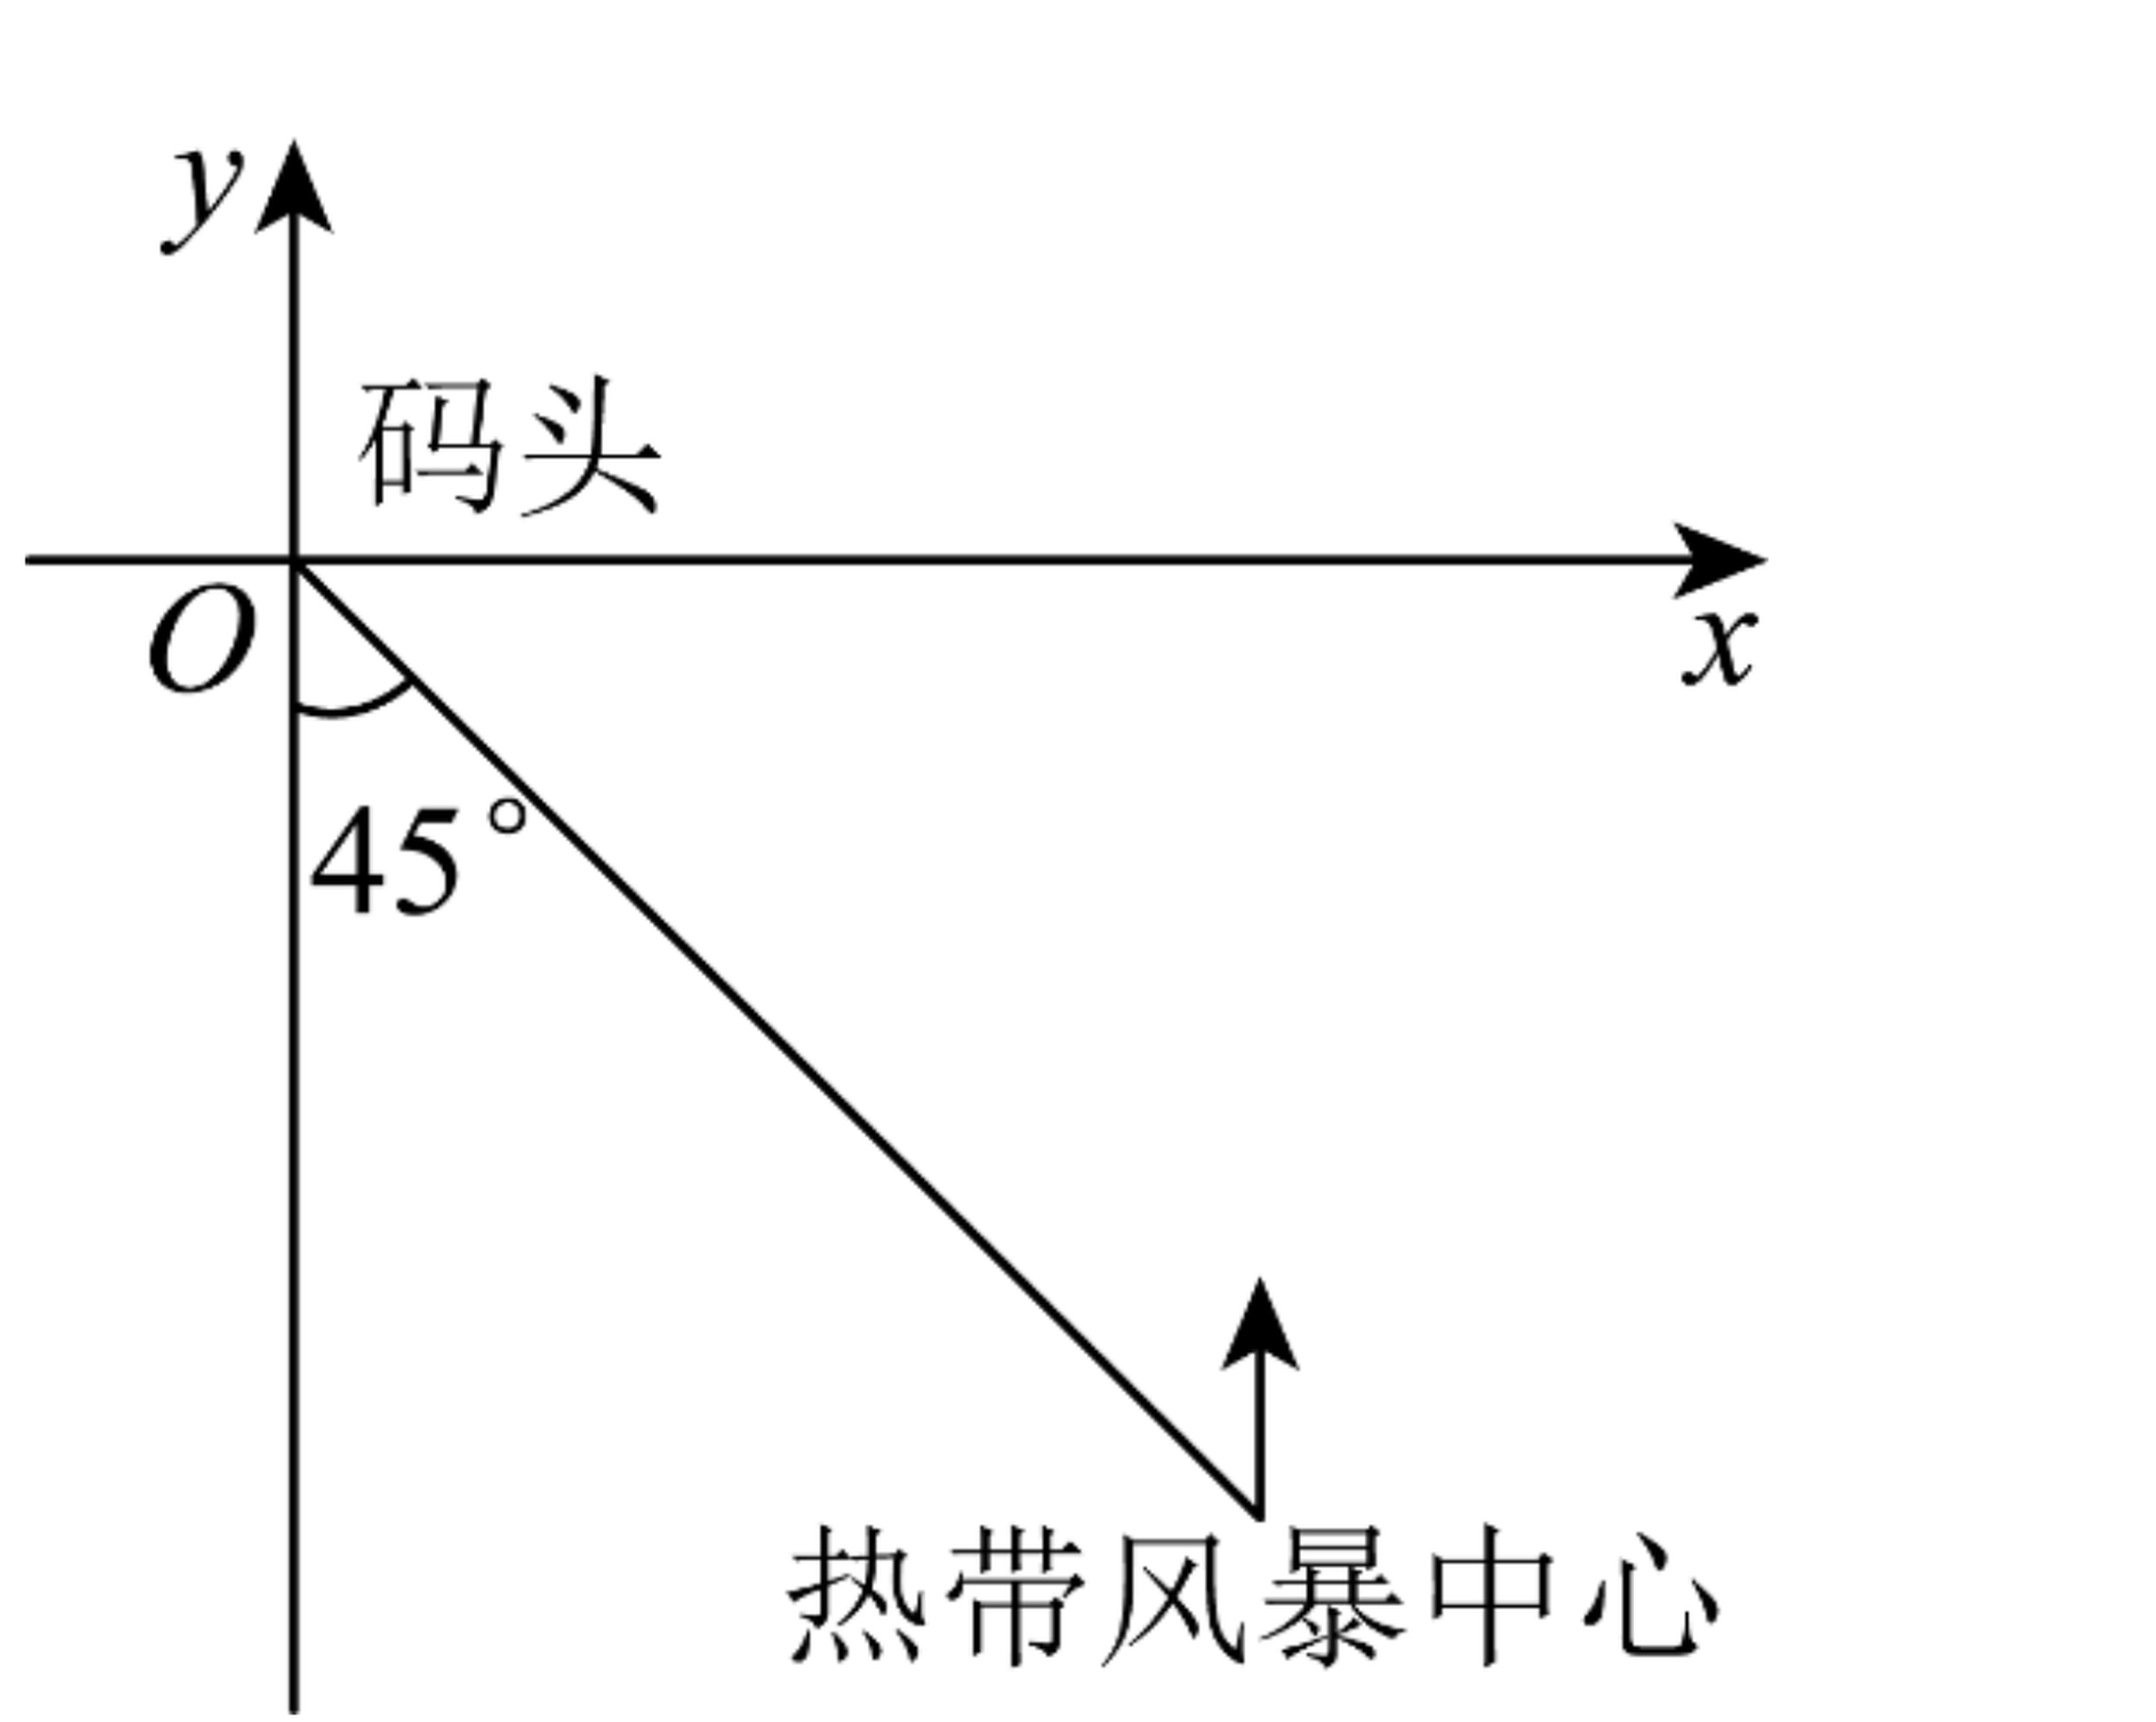
\includegraphics[width=0.36\textwidth]{figures/gao123_q5.png}
\end{center}

\ifanswer
\solbegin
\step{设风暴中心的坐标为 $(a,b)$，}
\step{由题意得 $a=400\sqrt2\times\cos45^\circ=400$，当 $a^2+b^2=400^2+b^2<500^2$，}% 原卷 $a^2$ 与 $400^2$ 并用，照录
\step{即 $-300<b<300$ 时，码头将受到风暴影响，}
\step{$\dfrac{300-(-300)}{20}=30h$，则码头受到风暴影响的时长为 30 小时，}
\step{所以由预报估计，该码头将受到热带风暴的影响时长大约为 30 小时.}
\solend
\fi

\item 已知 $a$、$b$、$c$ 为常数，若不等式 $\dfrac{ax-b}{x-c}\geqslant0$ 的解集为 $[-1,1)$，则不等式 $ax+b<0$ 的解集为\blankline[4.4em].

\ifanswer
\solbegin
\step{不等式 $\dfrac{ax-b}{x-c}\geqslant0$ 可化为 $(ax-b)(x-c)\geqslant0$ 且 $x-c\neq0$，}
\step{即 $a\left(x-\dfrac ba\right)(x-c)\geqslant0$ 且 $x\neq c$，}
\step{因为不等式 $\dfrac{ax-b}{x-c}\geqslant0$ 的解集为 $[-1,1)$，所以 $a<0$，且 $\dfrac ba=-1$,$c=1$，}
\step{即 $b=-a$，所以不等式 $ax+b<0$ 可化为 $ax-a<0$，又因为 $a<0$，所以 $x-1>0$，}
\step{解得 $x>1$，所以不等式 $ax+b<0$ 的解集为 $(1,+\infty)$.}
\solend
\fi

\item 已知实数 $a$、$b$ 满足 $ab=32$，且 $\log_2a=\log_b16$，则 $a+b$ 的值为\blankline[4.4em].

\ifanswer
\solbegin
\step{由 $\log_2a=\log_b16$，得 $\log_2a=\dfrac{\log_216}{\log_2b}$，则 $\log_2a\cdot\log_2b=4$，}
\step{由 $ab=32$，得 $\log_2a+\log_2b=\log_2ab=5$，}
\step{得 $\log_2a=1$,$\log_2b=4$ 或 $\log_2a=4$,$\log_2b=1$，}
\step{因此 $a=2$,$b=16$ 或 $a=16$,$b=2$，所以 $a+b=18$.}
\solend
\fi

\item 已知实数 $a$、$b$ 满足 $-3<a+2b<2$，$-1<2a-b<4$，则 $a+b$ 的取值范围为\blankline[4.4em].

\ifanswer
\solbegin
\step{设 $a+b=m(a+2b)+n(2a-b)=(m+2n)a+(2m-n)b$，}
\step{所以 $\begin{cases}m+2n=1\\2m-n=1\end{cases}$，解得 $n=\dfrac15$,$m=\dfrac35$，所以 $a+b=\dfrac35(a+2b)+\dfrac15(2a-b)$，}
\step{因为 $-3<(a+2b)<2$，$-1<2a-b<4$，}
\step{所以 $-\dfrac95<\dfrac35(a+2b)<\dfrac65$，$-\dfrac15<\dfrac15(2a-b)<\dfrac45$，}
\step{相加得 $-2<\dfrac35(a+2b)+\dfrac15(2a-b)<2$，即 $-2<a+b<2$，}
\step{故 $a+b$ 的取值范围为 $(-2,2)$.}
\solend
\fi

\item 存在 $x\in\R$ 使不等式 $\lvert2x-a\rvert<\lvert2a-1\rvert-2\lvert x\rvert$ 成立，则实数 $a$ 的取值范围是\blankline[4.4em].

\ifanswer
\solbegin
\step{存在 $x\in\R$，不等式 $\lvert2x-a\rvert<\lvert2a-1\rvert-2\lvert x\rvert$ 成立，}
\step{变形即 $\lvert2x-a\rvert+2\lvert x\rvert<\lvert2a-1\rvert$ 成立，}
\step{由于 $\lvert2x-a\rvert+\lvert2x\rvert\geqslant\lvert(2x-a)-2x\rvert=\lvert a\rvert$，当且仅当 $2x(2x-a)\leqslant0$ 时取等号，}
\step{因此有 $\lvert a\rvert<\lvert2a-1\rvert$，两边平方 $a^2<(2a-1)^2$，解得 $a>1$ 得 $a<\dfrac13$，}% 原卷“解得 a>1 得 a<1/3”，照录
\step{即实数 $a$ 的取值范围是 $\left(-\infty,\dfrac13\right)\cup(1,+\infty)$.}
\solend
\fi

\item 已知集合 $A=\{(x,y)\mid x^2+mx-y+2=0\}$，$B=\{(x,y)\mid x-y+1=0,0\leqslant x\leqslant3\}$，若集合 $A\cap B$ 的子集个数为 $2$，则实数 $m$ 的取值范围为\blankline[4.4em].

\ifanswer
\solbegin
\step{因为集合 $A\cap B$ 的子集个数为 $2$，所以 $A\cap B$ 的元素有一个，}
\step{即 $\begin{cases}x^2+mx-y+2=0\\x-y+1=0\end{cases}$ 在 $x\in[0,3]$ 上只有一个解，}
\step{即 $x^2+(m-1)x+1=0$ 在 $[0,3]$ 上只有一个解，}
\step{即 $1-m=x+\dfrac1x$ 在 $[0,3]$ 上只有一个解，}
\step{结合对勾函数的性质得 $1-m=2$ 或 $1-m>\dfrac{10}{3}$，解得 $m=-1$ 或 $m<-\dfrac73$.}
\solend
\fi

\item $[x]$ 表示不超过 $x$ 的最大整数，则集合 $A=\left\{y\,\middle\vert\,y=\left[\dfrac{x^2}{100}\right],x=1,2,3,\cdots,100\right\}$ 中的元素个数为\blankline[4.4em].

\ifanswer
\solbegin
\step{记 $a_k=\left[\dfrac{k^2}{100}\right](k=1,2,\cdots,100)$，$a_k$ 随 $k$ 增大而单调不减.}
\step{当 $k\geqslant50$ 时，$\dfrac{(k+1)^2}{100}-\dfrac{k^2}{100}=\dfrac{2k+1}{100}\geqslant\dfrac{101}{100}>1$，所以 $a_{k+1}\geqslant a_k+1$，}
\step{即 $a_{50}$、$a_{51}$、$\cdots$、$a_{100}$ 两两互异.}
\step{又 $a_{50}=\left[\dfrac{2500}{100}\right]=25$、$a_{100}=100$，这一段共 $100-50+1=51$ 个互异的值，}
\step{且都大于等于 $25$.}
\step{当 $k\leqslant49$ 时，$\dfrac{(k+1)^2}{100}-\dfrac{k^2}{100}=\dfrac{2k+1}{100}\leqslant\dfrac{99}{100}<1$，即 $a_k$ 每次至多增加 $1$；}
\step{又 $a_1=0$、$a_{49}=\left[\dfrac{2401}{100}\right]=24$，}
\step{故 $a_1$、$a_2$、$\cdots$、$a_{49}$ 依次取遍 $0$，$1$，$2$，$\cdots$，$24$，共 $25$ 个值.}
\step{两段取值范围互不重叠（前段不超过 $24$、后段不小于 $25$），}
\step{所以集合 $A$ 中共有 $25+51=76$ 个元素.}
\solend
\fi

\item 若实数 $a$、$b$、$c$ 满足 $\dfrac1{2^a}+\dfrac1{2^b}=1$，$\dfrac1{2^{a+b}}+\dfrac1{2^{b+c}}+\dfrac1{2^{a+c}}=1$，则 $c$ 的最大值是\blankline[4.4em].

\ifanswer
\solbegin
\step{因为 $\dfrac1{2^a}+\dfrac1{2^b}=1$，}
\step{由基本不等式得 $1=\dfrac1{2^a}+\dfrac1{2^b}\geqslant2\sqrt{\dfrac1{2^a}\cdot\dfrac1{2^b}}$（当且仅当 $a=b=1$ 时取等号），}
\step{所以 $\dfrac1{2^a}\cdot\dfrac1{2^b}\leqslant\dfrac14$，所以 $-\dfrac1{2^a}\cdot\dfrac1{2^b}\geqslant-\dfrac14$，}% 原卷带负号起论，照录
\step{因为 $\dfrac1{2^{a+b}}+\dfrac1{2^{b+c}}+\dfrac1{2^{a+c}}=1$，$\dfrac1{2^{b+c}}+\dfrac1{2^{a+c}}=\dfrac1{2^c}\left(\dfrac1{2^a}+\dfrac1{2^b}\right)=\dfrac1{2^c}$，}
\step{所以 $\dfrac1{2^c}=1-\dfrac1{2^{a+b}}\geqslant\dfrac34$，所以 $2^c\leqslant\dfrac43$，所以 $c\leqslant\log_2\dfrac43=2-\log_23$，}
\step{故 $c$ 的最大值是 $2-\log_23$.}
\solend
\fi

\end{enumerate}

\bigsec{二、选择题}

\begin{enumerate}
\setcounter{enumi}{12}

\item 下列运用等式或不等式的性质变形中，正确的是\mbox{（\quad）}

\keepwithprev
A. 如果 $a=b$，那么 $\dfrac ac=\dfrac bc$\qquad\qquad B. 如果 $\dfrac1a<\dfrac1b<0$，那么 $a-\dfrac1a>b-\dfrac1b$

C. 如果 $a>b$，那么 $\dfrac1a<\dfrac1b$\qquad\qquad D. 如果 $a>b>0$，$m\in\R$，那么 $\dfrac ba<\dfrac{b+m}{a+m}$

\ifanswer
\solbegin
\step{对于 $A$，若 $c=0$，$A$ 错误；}
\step{对于 $B$，若 $\dfrac1a<\dfrac1b<0$，则 $0>a>b$，$-\dfrac1a>-\dfrac1b>0$，}
\step{所以 $a-\dfrac1a>b-\dfrac1b$，$B$ 正确；}
\step{对于 $C$，$a>0$，$b<0$ 时，$C$ 错误；}
\step{对于 $D$，$\dfrac{b+m}{a+m}-\dfrac ba=\dfrac{ab+am}{a(a+m)}-\dfrac{ab+bm}{a(a+m)}=\dfrac{(a-b)m}{a(a+m)}$，}
\step{因为 $a>b>0$，所以 $a-b>0$，但 $m$、$a+m$ 的符号不确定，}
\step{当 $m=0$ 时，$\dfrac ba=\dfrac{b+m}{a+m}$，}
\step{当 $m(a+m)>0$ 时，$\dfrac ba<\dfrac{b+m}{a+m}$，当 $m(a+m)<0$ 时，$\dfrac ba>\dfrac{b+m}{a+m}$，$D$ 错误.}
\step{故选 $B$.}
\solend
\fi

\item “$a>b$”的一个必要非充分条件是\mbox{（\quad）}

\keepwithprev
A. $ac^2>bc^2$\qquad\quad B. $2^a>2^b$\qquad\quad C. $\left(\dfrac12\right)^{a-b}\leqslant1$\qquad\quad D. $a^3>b^3$

\ifanswer
\solbegin
\step{即“$a>b$”能推出选项，但选项不能推出“$a>b$”，故选 $C$.}
\solend
\fi

\item 若 $A=\left\{x\,\middle\vert\,x=\dfrac k6+1,k\in\Z\right\}$，$B=\left\{x\,\middle\vert\,x=\dfrac k3+\dfrac12,k\in\Z\right\}$，$C=\left\{x\,\middle\vert\,x=\dfrac{2k}{3}+\dfrac12,k\in\Z\right\}$，则这三个集合间的关系是\mbox{（\quad）}

\keepwithprev
A. $A\subseteq B\subseteq C$\qquad\quad B. $A\subseteq C\subseteq B$\qquad\quad C. $C\subseteq B\subseteq A$\qquad\quad D. $C\subseteq A\subseteq B$

\ifanswer
\solbegin
\step{若 $x\in C$，则存在 $k_0\in\Z$，使 $x=\dfrac{2k_0}{3}+\dfrac12$，}
\step{又 $2k_0\in\Z$，所以 $x\in B$，故 $C\subseteq B$，}
\step{若 $x\in B$，则存在 $k_1\in\Z$，使 $x=\dfrac{k_1}{3}+\dfrac12=\dfrac{2k_1-3}{6}+1$，}
\step{又 $2k_1-3\in\Z$，所以 $x\in A$，故 $B\subseteq A$，}
\step{又 $\dfrac43\in A$，$\dfrac43\notin B$，$\dfrac56\in B$，$\dfrac56\notin C$，所以 $C\subseteq B\subseteq A$，故选 $C$.}
\solend
\fi

\item 集合 $S=\{x\mid(x+a)(x^2+bx+c)=0\}$，$T=\{x\mid(ax+1)(cx^2+bx+1)=0\}$，其中 $a$、$b$、$c$ 为实数，若 $\lvert S\rvert$、$\lvert T\rvert$ 分别表示 $S$、$T$ 的元素个数，则下列结论中一定成立的是\mbox{（\quad）}

\keepwithprev
A. 若 $\lvert T\rvert=0$，则 $\lvert S\rvert=1$\qquad\qquad B. 若 $\lvert S\rvert=1$，则 $\lvert T\rvert=1$

C. 若 $\lvert S\rvert=2$，则 $\lvert T\rvert=2$\qquad\qquad D. 若 $\lvert T\rvert=3$，则 $\lvert S\rvert=2$

\ifanswer
\solbegin
\step{令 $f(x)=(x+a)(x^2+bx+c)$,$g(x)=(ax+1)(cx^2+bx+1)$，}
\step{对于选项 A，当 $\lvert T\rvert=0$ 时，方程 $g(x)=(ax+1)(cx^2+bx+1)=0$ 无实根，}
\step{当 $a=b=c=0$ 时，$f(x)=x^3$，由 $f(x)=0$ 得 $x=0$，此时 $\lvert S\rvert=1$；}
\step{当 $a=0$,$b^2-4c<0$ 时，$f(x)=x(x^2+bx+c)$，由 $f(x)=0$ 得 $x=0$，}
\step{此时 $\lvert S\rvert=1$，所以选项 A 正确；}
\step{对于选项 B，若 $\lvert S\rvert=1$，则 $f(x)=(x+a)(x^2+bx+c)=0$ 有且只有一根，}
\step{又 $x=-a$ 一定是 $f(x)=0$ 的根，所以 $\triangle=b^2-4c<0$，}
\step{又 $\triangle=b^2-4c<0$ 且 $a=0$ 时，$g(x)=(ax+1)(cx^2+bx+1)=0$ 无解，}
\step{此时 $\lvert T\rvert=0$，所以选项 B 错误，}
\step{对于选项 C，若 $\lvert S\rvert=2$ 时，则 $f(x)=(x+a)(x^2+bx+c)=0$ 有且只有 $2$ 根，}
\step{又 $x=-a$ 一定是 $f(x)=0$ 的根，}
\step{所以 $\triangle=b^2-4c=0$ 且 $a^2+ab+c\neq0$ 或 $\triangle=b^2-4c>0$ 且 $a^2+ab+c=0$，}
\step{当 $a=0$ 时，存在 $b$,$c$，使 $\triangle=b^2-4c=0$ 且 $a^2+ab+c\neq0$，}
\step{此时 $g(x)=(ax+1)(cx^2+bx+1)=0$ 只有一根，所以选项 C 错误，}
\step{对于选项 D，当 $\lvert T\rvert=3$ 时，方程 $g(x)=(ax+1)(cx^2+bx+1)=0$ 有三个根，}
\step{所以 $a\neq0$,$c\neq0$,$b^2-4c>0$，}
\step{设 $x_0$ 为 $g(x)=0$ 的一个根，即 $(ax_0+1)(cx_0^2+bx_0+1)=0$，}
\step{则 $x_0\neq0$，且 $f\left(\dfrac1{x_0}\right)=\left(\dfrac1{x_0}+a\right)\left(\dfrac1{x_0^2}+\dfrac1{x_0}b+c\right)=\dfrac1{x_0^3}g(x_0)=0$，}
\step{所以 $\dfrac1{x_0}$ 为方程 $f(x)=0$ 的根，故 $f(x)=0$ 有三个根，即 $\lvert T\rvert=3$ 时，}
\step{必有 $\lvert S\rvert=3$，所以选项 D 错误，}
\step{故选 $A$.}
\solend
\fi

\end{enumerate}

% 第 17 题是解答题第一题且带文氏图，守卫放在 \bigsec 之前，连节标题一起量页高
\needvspace{7cm}
\bigsec{三、解答题}

\begin{enumerate}
\setcounter{enumi}{16}

\item 设全集 $U=\R$，集合 $A=\{x\mid-2\leqslant x\leqslant4\}$，$B=\{x\mid x<-6$ 或 $x\geqslant2\}$.

（1）求图中阴影部分表示的集合；

（2）已知集合 $C=\{x\mid10-a<x<2a+1\}$，若 $\overline B\cap C=\varnothing$，求 $a$ 的取值范围.

\begin{center}
% 图取原卷截图（第 7 页题干右侧）、去水印后 2× LANCZOS 放大，本稿移至题干之后
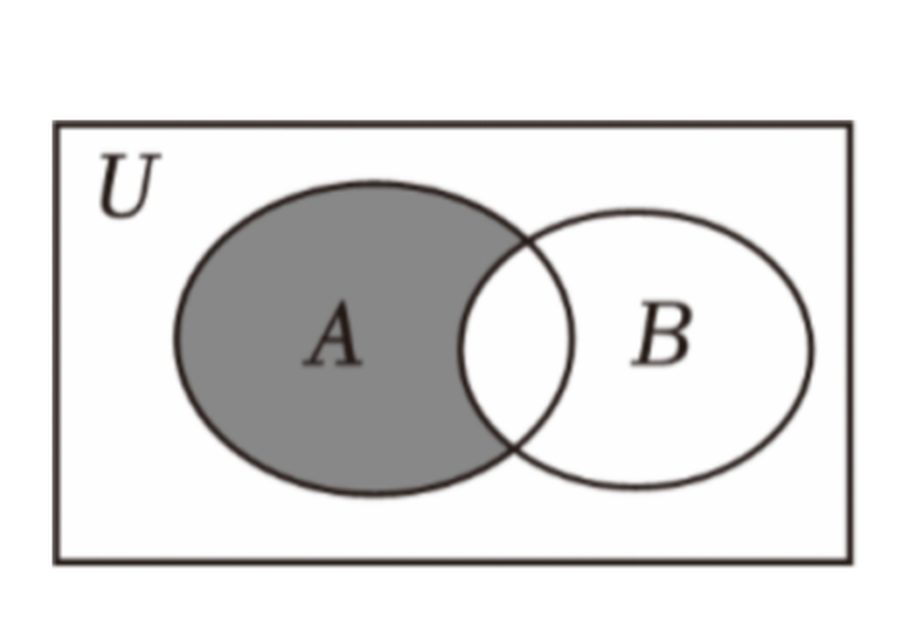
\includegraphics[width=0.34\textwidth]{figures/gao123_q17.png}
\end{center}

\ifanswer
\solbegin
\step{（1）$A\cap B=\{x\mid2\leqslant x\leqslant4\}$，}
\step{则图中阴影部分表示 $\overline{A\cap B}=\{x\mid-2\leqslant x<2\}$.}% 原卷把上划线盖在整个 $A\cap B$ 上，照录
\step{（2）由题意得 $\overline B=\{x\mid-6\leqslant x<2\}$，$C\subseteq B$，}
\step{所以当 $C=\varnothing$ 时，$10-a\geqslant2a+1$，解得 $a\leqslant3$，符合题意；}
\step{当 $C\neq\varnothing$ 时，$\begin{cases}10-a<2a+1\\2a+1\leqslant-6\end{cases}$ 或者 $\begin{cases}10-a<2a+1\\10-a\geqslant2\end{cases}$，}
\step{此时不等式组 $\begin{cases}10-a<2a+1\\2a+1\leqslant-6\end{cases}$ 无解，}
\step{不等式组 $\begin{cases}10-a<2a+1\\10-a\geqslant2\end{cases}$ 的解集为 $3<a\leqslant8$，}
\step{综上，$a$ 的取值范围为 $\{a\mid a\leqslant8\}$.}
\solend
\fi

\item (1) 求不等式：$\lvert x-1\rvert+\lvert x-2\rvert\leqslant5$ 的解集.

(2) 当 $m<1$ 时，解关于 $x$ 的不等式 $\dfrac{m(x-3)}{x+2}>1$.

\ifanswer
\solbegin
\step{(1) 当 $x<1$ 时，$\lvert x-1\rvert+\lvert x-2\rvert\leqslant5\Leftrightarrow-x+1+2-x\leqslant5$，}
\step{解得 $-1\leqslant x<1$；}
\step{当 $1\leqslant x\leqslant2$ 时，$\lvert x-1\rvert+\lvert x-2\rvert\leqslant5\Leftrightarrow x-1+2-x=1\leqslant5$ 恒成立，}
\step{所以 $1\leqslant x\leqslant2$；}
\step{当 $x>2$ 时，$\lvert x-1\rvert+\lvert x-2\rvert\leqslant5\Leftrightarrow x-1+x-2=2x-3\leqslant5$，}
\step{解得 $2<x\leqslant4$.}
\step{综上所述，不等式 $\lvert x-1\rvert+\lvert x-2\rvert\leqslant5$ 的解集为 $[-1,4]$.}
\step{(2) 原不等式变成 $\dfrac{(m-1)x-(3m+2)}{x+2}>0$，$n<1$，所以 $n-1<0$，}% 原卷作 $n<1$、$n-1<0$，与题设 $m<1$ 字母不一致，照录
\step{所以原不等式变成 $\dfrac{x-\dfrac{3m+2}{m-1}}{x+2}<0$，$\dfrac{3m+2}{m-1}-(-2)=\dfrac{5m}{m-1}$，}
\step{所以 $m<0$ 时，$\dfrac{5m}{m-1}>0$，$\dfrac{3m+2}{m-1}>-2$，}
\step{原不等式的解集为 $\left(-2,\dfrac{3m+2}{m-1}\right)$；}
\step{$m=0$ 时，原不等式变成 $1<0$，无解；}
\step{$0<m<1$ 时，$\dfrac{5m}{m-1}<0$，$\dfrac{3m+2}{m-1}<-2$，}
\step{原不等式的解集为 $\left(\dfrac{3m+2}{m-1},-2\right)$.}
\solend
\fi

\item 在园林博览会上，某公司带来了一种智能设备供采购商洽谈采购，并决定大量投放市场，已知该种设备年固定研发成本为 $50$ 万元，每生产一台需另投入 $100$ 元，设该公司一年内生产该设备 $x$ 万台且全部售完，每万台的销售收入 $G(x)$（万元）与年产量 $x$（万台）满足如下关系式：$G(x)=\begin{cases}180-x,0<x\leqslant20\\80+\dfrac{2000}{x}-\dfrac{8000}{x(x-1)},x>20\end{cases}$.

(1) 写出年利润 $W(x)$（万元）关于年产量 $x$（万台）的函数解析式；（利润 $=$ 销售收入 $-$ 成本）

(2) 当年产量为多少万台时，该公司获得的年利润最大，并求出最大利润.

\ifanswer
\solbegin
\step{(1) $W(x)=xG(x)-50-100x=\begin{cases}-50+80x-x^2,0<x\leqslant20\\-20x+1950-\dfrac{8000}{x-1},x>20\end{cases}$；}
\step{(2) 当 $0<x\leqslant20$ 时，$W(x)=-50+80x-x^2=-(x-40)^2+1550$，}
\step{由函数性质得当 $x\leqslant40$ 时严格增，所以当 $x=20$ 时，$W(x)_{max}=1150$，}
\step{当 $x>20$ 时，$W(x)=-20x+1950-\dfrac{8000}{x-1}=-20\left[(x-1)+\dfrac{400}{x-1}\right]+1930$，}
\step{$W(x)=-20\left[(x-1)+\dfrac{400}{x-1}\right]+1930\leqslant-20\times2\sqrt{(x-1)\cdot\dfrac{400}{x-1}}+1930$}
\step{$=1130$，当且仅当 $x-1=\dfrac{400}{x-1}$，即 $x=21$ 时取等号，}
\step{所以 $W(x)_{max}=1130$，}
\step{因为 $1150>1130$，所以当 $x=20$ 时，$W(x)_{max}=1150$，}
\step{即当年产量为 $20$ 万台时，该公司获得的年利润最大，}
\step{最大利润为 $1150$ 万元.}
\solend
\fi

\item 关于 $x$ 的方程 $(x^2-1)^2-2k\lvert x^2-1\rvert+k+1=0(k\in\R)$.

(1) 若方程无实根，求 $k$ 的取值范围；

(2) 若方程有 $4$ 个不等实根，求 $k$ 的取值范围；

(3) 若 $k=a+b$，且满足 $\dfrac1{a+2b}+\dfrac1{a+3}=\dfrac12$，$a>0$，$b>0$，试判断方程根的个数.

\ifanswer
\solbegin
\step{(1) 关于 $x$ 的方程 $(x^2-1)^2-2k\lvert x^2-1\rvert+k+1=0(k\in\R)$，}
\step{令 $t=\lvert x^2-1\rvert$，则 $t\geqslant0$，则原方程转化为 $t^2-2kt+k+1=0(*)$，}
\step{因为关于 $x$ 的方程 $(x^2-1)^2-2k\lvert x^2-1\rvert+k+1=0(k\in\R)$ 无实根，}
\step{所以 $(*)$ 式无实根或实根均小于零，令 $f(t)=t^2-2kt+k+1$，}
\step{①若 $(*)$ 式无实根，则 $\triangle<0$，解得 $\dfrac{1-\sqrt5}{2}<k<\dfrac{1+\sqrt5}{2}$，}
\step{②两根均为负，则 $\begin{cases}\Delta\geqslant0\\t_{\text{对}}=k<0\\f(0)>0\end{cases}$，解得 $-1<k\leqslant\dfrac{1-\sqrt5}{2}$，}
\step{综合①②，得 $k$ 的取值范围是 $\left(-1,\dfrac{1+\sqrt5}{2}\right)$；}
\step{(2) 作函数 $t=\lvert x^2-1\rvert$ 的图象，}
\begin{center}
% 图取原卷截图（第 11 页解析内）、去水印后 2× LANCZOS 放大，仅答案版出
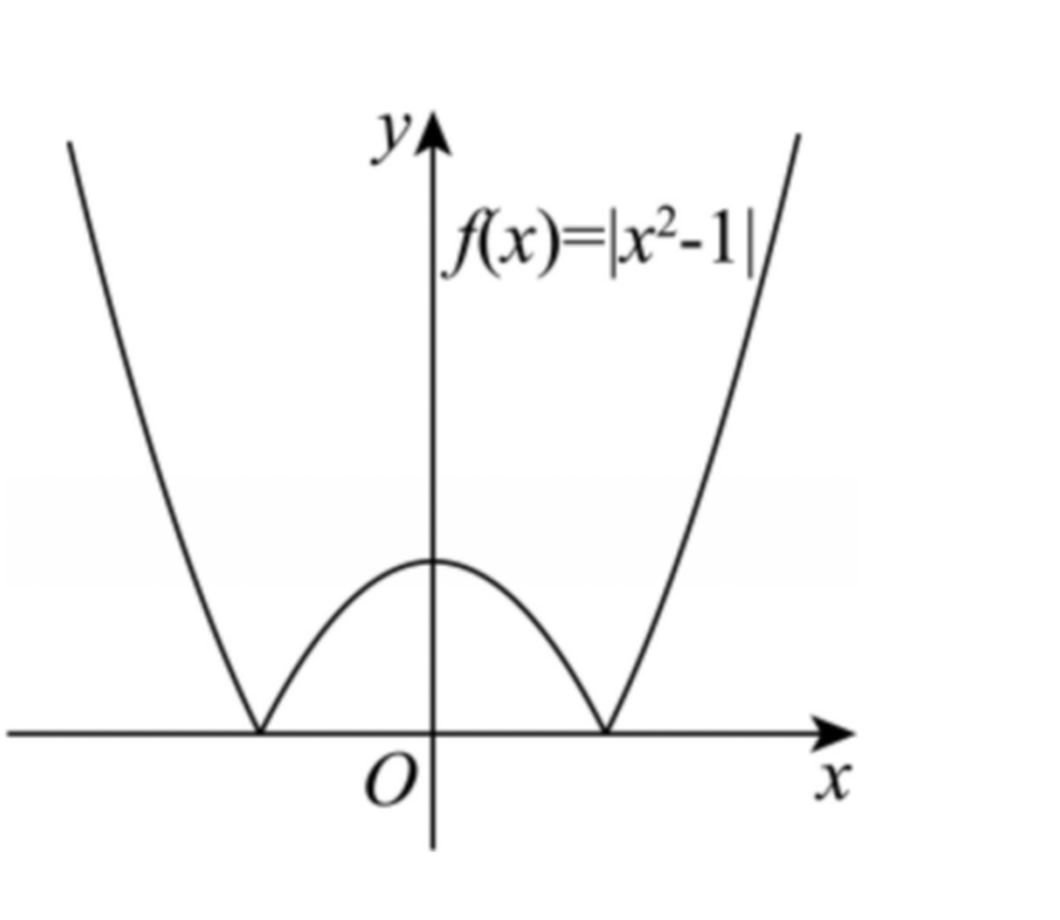
\includegraphics[width=0.40\textwidth]{figures/gao123_q20.png}
\end{center}
\step{$t=0$ 或 $t>1$ 时，每一个 $t$ 值对应 $2$ 个不同的 $x$ 值，}
\step{$t=1$ 时一个 $t$ 值对应 $3$ 个不同的 $x$ 值，}
\step{$0<t<1$ 时一个 $t$ 值对应 $4$ 个不同的 $x$ 值，}
\step{要使原方程有四个不等实根，}
\step{①$(*)$ 式一根为零，另一根大于 $1$，无解；}
\step{②$(*)$ 有两不等根且两根均大于 $1$，则 $\begin{cases}\Delta>0\\t_{\text{对}}=k>1\\f(1)>0\end{cases}$，解得 $\dfrac{1+\sqrt5}{2}<k<2$；}
\step{④$(*)$ 式有 $1$ 实根在 $(0,1)$ 之间，另一根小于零，}% 原卷由 ② 直接跳到 ④，缺 ③，照录
\step{则 $\begin{cases}f(0)<0\\f(1)>0\end{cases}$，所以 $\begin{cases}k+1<0\\2-k>0\end{cases}$，解得 $k<-1$，}
\step{综上所述，$k$ 取值范围为 $(-\infty,-1)\cup\left(\dfrac{1+\sqrt5}{2},2\right)$；}
\step{(3) 因为 $\dfrac1{a+2b}+\dfrac1{a+3}=\dfrac{a+2b+a+3}{(a+2b)(a+3)}=\dfrac{2(a+b)+3}{(a+2b)(a+3)}=\dfrac12$，}
\step{所以 $2(a+b)+3=\dfrac12(a+2b)(a+3)$，}
\step{因为 $a$、$b$ 为正实数，所以 $\dfrac12=\dfrac1{a+2b}+\dfrac1{a+3}\geqslant2\sqrt{\dfrac1{a+2b}\times\dfrac1{a+3}}$，}
\step{得 $\dfrac1{16}\geqslant\dfrac1{a+2b}\times\dfrac1{a+3}$，即 $(a+2b)(a+3)\geqslant16$，}
\step{所以 $2(a+b)+3\geqslant8$，即 $a+b\geqslant\dfrac52$，}
\step{当且仅当 $\dfrac1{a+2b}=\dfrac1{a+3}$ 即 $a=1$,$b=\dfrac32$ 时取等号，}
\step{故 $k\geqslant\dfrac52$，此时有 $\begin{cases}\Delta>0\\t_{\text{对}}=k>1\\f(0)>0,f(1)<0\end{cases}$，}
\step{故 $(*)$ 式有两不等实根且一根在 $(0,1)$ 之间，另一根大于 $1$，}
\step{故原方程有 $6$ 个实根.}
\solend
\fi

\item 设 $n$ 是不小于 $3$ 的正整数，集合 $S_n=\{(a_1,a_2,\cdots,a_n)\mid a_i\in\{0,1\},i=1,2,\cdots,n\}$，对于集合 $S_n$ 中任意两个元素 $A=(a_1,a_2,\cdots,a_n)$，$B=(b_1,b_2,\cdots,b_n)$.

定义 1：$A\cdot B=n-(\lvert a_1-b_1\rvert+\lvert a_2-b_2\rvert+\cdots+\lvert a_n-b_n\rvert)$，

定义 2：若 $A\cdot B=0$，则称互为相反元素，记作 $A=\overline B$ 或 $B=\overline A$.

(1) 若 $n=3$，$A=(0,1,0)$，$B=(1,1,0)$，试写出 $\overline A$、$\overline B$ 以及 $A\cdot B$ 的值；

(2) 若 $A$、$B\in S_n$，$A=(a_1,a_2,\cdots,a_n)$，$B=(b_1,b_2,\cdots,b_n)$，证明：$A\cdot B+\overline A\cdot B=n$；

(3) 设 $k$ 是小于 $n$ 的正奇数，至少含有两个元素的集合 $M\subseteq S_n$，且对于集合 $M$ 中任意两个不相同的元素 $A=(a_1,a_2,\cdots,a_n)$，$B=(b_1,b_2,\cdots,b_n)$，都有 $A\cdot B=n-k$，试求集合 $M$ 中元素个数的所有可能值.

\ifanswer
\solbegin
\step{(1) $\overline A=(1,0,1)$,$\overline B=(0,0,1)$,$\overline A\cdot\overline B=2$；}
\step{(2) 设 $A=(a_1,a_2,\cdots,a_n)$,$B=(b_1,b_2,\cdots,b_n)$,$\overline A=(x_1,x_2,\cdots,x_n)$，}
\step{由 $a_i$、$b_i$、$x_i\in\{0,1\}$，$i=1,2,\cdots,n$，得 $\lvert a_i-x_i\rvert\leqslant1$，$i=1,2,\cdots,n$，}
\step{所以 $\lvert a_1-x_1\rvert+\lvert a_2-x_2\rvert+\cdots+\lvert a_i-x_i\rvert\leqslant n$，}% 原卷末项下标作 $i$，照录
\step{当且仅当 $\lvert a_i-x_i\rvert=1$，$i=1,2,\cdots,n$，}
\step{即 $x_i=1-a_i$，$i=1,2,\cdots,n$ 时取等号.}
\step{由题意得 $A\cdot\overline A=n-(\lvert a_1-x_1\rvert+\lvert a_2-x_2\rvert+\cdots+\lvert a_n-x_n\rvert)=0$，}
\step{即 $\lvert a_1-x_1\rvert+\lvert a_2-x_2\rvert+\cdots+\lvert a_n-x_n\rvert=n$，}
\step{所以 $x_i=1-a_i$，$i=1,2,\cdots,n$，}
\step{$A\cdot B+\overline A\cdot B=2n-\sum\limits_{i=1}^n[\lvert a_i-b_i\rvert+(1-a_i)-b_i]$}
\step{$=2n-\sum\limits_{i=1}^n(\lvert1-b_i\rvert+\lvert0-b_i\rvert)=2n-\sum\limits_{i=1}^n(1-b_i+b_i)=2n-n=n$；}
\step{(3) 假设 $A=(a_1,a_2,\cdots,a_n)$，$B=(b_1,b_2,\cdots,b_n)$，$C=(c_1,c_2,\cdots,c_n)$}
\step{为集合 $M$ 中的三个不相同的元素，}
\step{则 $A\cdot B=n-(\lvert a_1-b_1\rvert+\lvert a_2-b_2\rvert+\cdots+\lvert a_n-b_n\rvert)=n-k$，}
\step{即 $\lvert a_1-b_1\rvert+\lvert a_2-b_2\rvert+\cdots+\lvert a_n-b_n\rvert=k$，}
\step{又由题意得 $\lvert a_i-b_i\rvert=0$ 或 $1$，$i=1,2,\cdots,n$，}
\step{$\lvert a_1-b_1\rvert$、$\lvert a_2-b_2\rvert$、$\cdots$、$\lvert a_n-b_n\rvert$ 恰有 $k$ 个 $1$，$n-k$ 个 $0$，}
\step{设其中 $k$ 个等于 $1$ 的项以此为 $a_{m_1}-b_{m_1}$,$a_{m_2}-b_{m_2}$,$\cdots$,$a_{m_k}-b_{m_k}$，}
\step{$n-k$ 个等于 $0$ 的项为 $a_{m_{k+1}}-b_{m_{k+1}}$,$a_{m_{k+2}}-b_{m_{k+2}}$,$\cdots$,$a_{m_n}-b_{m_n}$，}
\step{由题意得 $A\cdot C=n-(\lvert a_1-c_1\rvert+\lvert a_2-c_2\rvert+\cdots+\lvert a_n-c_n\rvert)=n-k$，}
\step{所以 $\sum\limits_{i=1}^k\lvert a_{m_i}-c_{m_i}\rvert+\sum\limits_{j=k+1}^n\lvert a_{m_j}-c_{m_j}\rvert=k$ ①，}
\step{同理 $\sum\limits_{i=1}^k\lvert b_{m_i}-c_{m_i}\rvert+\sum\limits_{j=k+1}^n\lvert b_{m_j}-c_{m_j}\rvert=k$ ②，}
\step{因为 $\lvert a_{m_{k+1}}-b_{m_{k+1}}\rvert=\lvert a_{m_{k+2}}-b_{m_{k+2}}\rvert=\cdots=\lvert a_{m_n}-b_{m_n}\rvert=0$，}
\step{所以 $\sum\limits_{j=k+1}^n\lvert a_{m_j}-c_{m_j}\rvert=\sum\limits_{j=k+1}^n\lvert b_{m_j}-c_{m_j}\rvert$，}
\step{由①$-$②得 $\sum\limits_{i=1}^k(\lvert a_{m_i}-c_{m_i}\rvert-\lvert b_{m_i}-c_{m_i}\rvert)=0$，}
\step{又 $\sum\limits_{i=1}^k(\lvert a_{m_i}-c_{m_i}\rvert-\lvert b_{m_i}-c_{m_i}\rvert)=\sum\limits_{i=1}^k(\lvert1-c_{m_i}\rvert-\lvert0-c_{m_i}\rvert)=k-2\sum\limits_{i=1}^k c_{m_i}$}
\step{为奇数，与 $\sum\limits_{i=1}^k(\lvert a_{m_i}-c_{m_i}\rvert-\lvert b_{m_i}-c_{m_i}\rvert)=0$ 矛盾，所以假设不成立，}
\step{即集合 $M$ 中至多有两个元素，}
\step{当 $M=\{(1,1,\cdots,1,0,0,\cdots,0),(0,0,\cdots,0)\}$ 时符合题意，}
\step{所以集合 $M$ 中元素的个数只可能是 $2$.}
\solend
\fi

\end{enumerate}

\end{document}
"
% 紧凑版：xelatex "\def\iscompact{1}% 高一123_行知中学_10月月考.tex
%   —— 高一上数学“2026-2027 年行知中学高一上 10 月月考”（试卷版/答案版）
% 试卷版：xelatex 高一123_行知中学_10月月考.tex
% 答案版：xelatex "\def\isanswer{1}\input{高一123_行知中学_10月月考.tex}"
% 紧凑版：xelatex "\def\iscompact{1}\input{高一123_行知中学_10月月考.tex}"
%
% 原始材料：微信公众号“魔都数学加油站”文章，作者破晓，2026-11-09 17:52 发布；
% 连载“27学年高一123”，原文标题“27学年高一123——2026-2027年上海市行知中学高一上10月月考”；
% 原文链接：https://mp.weixin.qq.com/s/GV4SWBLUJrBhMQwo22FVzg。
% 正文为 14 张 PNG 页（第 7、9、11、13、14 页 2560×3620，其余 4762×6735），
% 题目下印有【答案】或【解析】，为讲评版。
% 题目、解析均据原图转录；卷面红色水印及公众号页脚未录入。
% 全卷 3 张插图：第 5 题的坐标示意图、第 17 题的文氏图（均属题干，三版都出）、
% 第 20 题 (2) 的 $t=\lvert x^2-1\rvert$ 图象（属解析，仅答案版出）；
% 都取原卷截图去水印、2× LANCZOS 放大，见 figures/gao123_q5.png、
% figures/gao123_q17.png、figures/gao123_q20.png。
%
% 卷首标题：原卷印作“2026-2027 年行知中学高一上 10 月月考”（公众号标题中的“上海市”
% 卷面标题行没有，本稿照卷面），年份区间按全稿惯例排 en dash；原卷未印副标题，本稿按题目内容
% 标为“集合与常用逻辑用语、不等式”（与 110／111／113／116／118／120 同）。
%
% 与原卷的排版差异：
%   ① 原文从第 3 题起，填空题编号为 3—12、选择题为 13—16、解答题为 17—21，本稿保留原题号；
%   ② 原卷每题下直接印【解析】／【答案】，本稿按全稿惯例置于答案版；第 3 题只印【答案】、
%      另提 \ans{}；选择题答案在解析末句“故选 …”，括号内留空；
%   ③ 原卷未印副标题，本稿按“知识模块”口径补出；
%   ④ 原卷填空横线按全稿惯例排为 \blankline[4.4em]；选择题括号排 \mbox{（\quad）}、
%      选项段前按惯例加 \keepwithprev；解答题不留作答区（原卷为讲评版，与 109—122 同）；
%   ⑤ 原卷数集排斜体 $R$／$Z$（第 9 题作粗体 $\mathbf{R}$），按全稿惯例改 \R／\Z；
%      绝对值按全稿惯例排 \lvert…\rvert，集合描述竖线排 \mid；单位 km、h 原卷排斜体，
%      本稿按正体照排；补集照原卷上划线排 \overline{B}、\overline{A}。
%
% 判别式与子集符号：第 16 题解析的 $\triangle=b^2-4c<0$、第 20 题 (1) ① 的 $\triangle<0$
%   均作等边、扁的 \triangle；第 20 题 ② 两处 cases 与 (3) 的 $\Delta\geqslant0$／$\Delta>0$
%   作等腰、高的 \Delta，逐处照录、不统一；第 15 题选项与第 17 题 (2) 的 $\subseteq$
%   印有下划线，照录 \subseteq。
%
% 原卷存疑照录：
%   第 4 题解析“若 $-\lvert a\rvert=0$，则 $a=0$，则 $A=\{0,-1,0\}$”以元素重复说明互异性；
%   第 5 题解析“当 $a^2+b^2=400^2+b^2<500^2$”等式左边 $a^2$ 与 $400^2$ 并用；
%   第 9 题解析“解得 $a>1$ 得 $a<\dfrac13$”（按平方不等式应为 $a>1$ 或 $a<\dfrac13$）；
%   第 12 题解析“所以 $-\dfrac1{2^a}\cdot\dfrac1{2^b}\geqslant-\dfrac14$”带负号起论；
%   第 17 题 (1) 解析把阴影部分（实为 $A\cap\overline B$）印作 $\overline{A\cap B}$；
%   第 18 题 (2) 解析作“$n<1$，所以 $n-1<0$”，与题设 $m<1$ 字母不一致；
%   第 20 题 (2) 的情形编号由 ①、② 直接跳到 ④（缺 ③）；
%   第 21 题 (2) 解析“$\lvert a_1-x_1\rvert+\cdots+\lvert a_i-x_i\rvert\leqslant n$”
%   末项下标作 $i$（按上下文应为 $n$）。以上均照录加注。
%
% 行数核对：逐题数 \step 条数，合计 176 条（Q3：0；Q4：6；Q5：5；Q6：5；Q7：4；
% Q8：6；Q9：5；Q10：5；Q11：10；Q12：6；Q13：9；Q14：1；Q15：5；Q16：21；
% Q17：8；Q18：14；Q19：10；Q20：26；Q21：30），与原卷印刷行逐题相等
% （cases 块作一个印刷行计）。第 3 题只印【答案】，提 \ans{}，不计入 \step 账。
%
\documentclass[a4paper,11pt]{article}
\usepackage{common}

\begin{document}

\examtitlest[3]{2026--2027 年行知中学高一上 10 月月考}{集合与常用逻辑用语、不等式}

\bigsec{一、填空题}

\begin{enumerate}
\setcounter{enumi}{2}

\item 写出命题“存在实数 $x$、$y$、$z$，使 $x<y$ 或 $y<z$.”的否定\blankline[4.4em].

\ifanswer
\ans{任意实数 $x$、$y$、$z$，使得 $x\geqslant y$ 且 $y\geqslant z$}
\fi

\item 若集合 $\{0,-1,2a\}=\{a-1,-\lvert a\rvert,a+1\}$，实数 $a$ 的值为\blankline[4.4em].

\ifanswer
\solbegin
\step{令 $A=\{0,-1,2a\}$,$B=\{a-1,-\lvert a\rvert,a+1\}$，}
\step{因为 $\{0,-1,2a\}=\{a-1,-\lvert a\rvert,a+1\}$，}
\step{若 $a-1=0$，则 $a=1$，则 $A=\{0,-1,2\}$,$B=\{0,-1,2\}$，满足要求；}
\step{若 $-\lvert a\rvert=0$，则 $a=0$，则 $A=\{0,-1,0\}$，不满足集合元素的互异性；}% 原卷以 $A=\{0,-1,0\}$ 说明互异性，照录
\step{若 $a+1=0$，则 $a=-1$，则 $A=\{0,-1,-2\}$,$B=\{0,-1,-2\}$，满足要求；}
\step{故实数 $a$ 的值为 $\pm1$.}
\solend
\fi

\needvspace{7cm}
\item 如图，据气象部门预报，在距离某码头南偏东 $45^\circ$ 方向 $400\sqrt2$ km 处的热带
风暴中心正在以 $20$km/h 的速度向正北方向移动，距风暴中心 $500$km 以内
的地区都将受到影响. 以上预报估计，该码头将受到热带风暴的影响时长大
约为\blankline[4.4em]$h$.

\begin{center}
% 图取原卷截图（第 1 页题干右侧）、去水印后 2× LANCZOS 放大，本稿移至题干之后
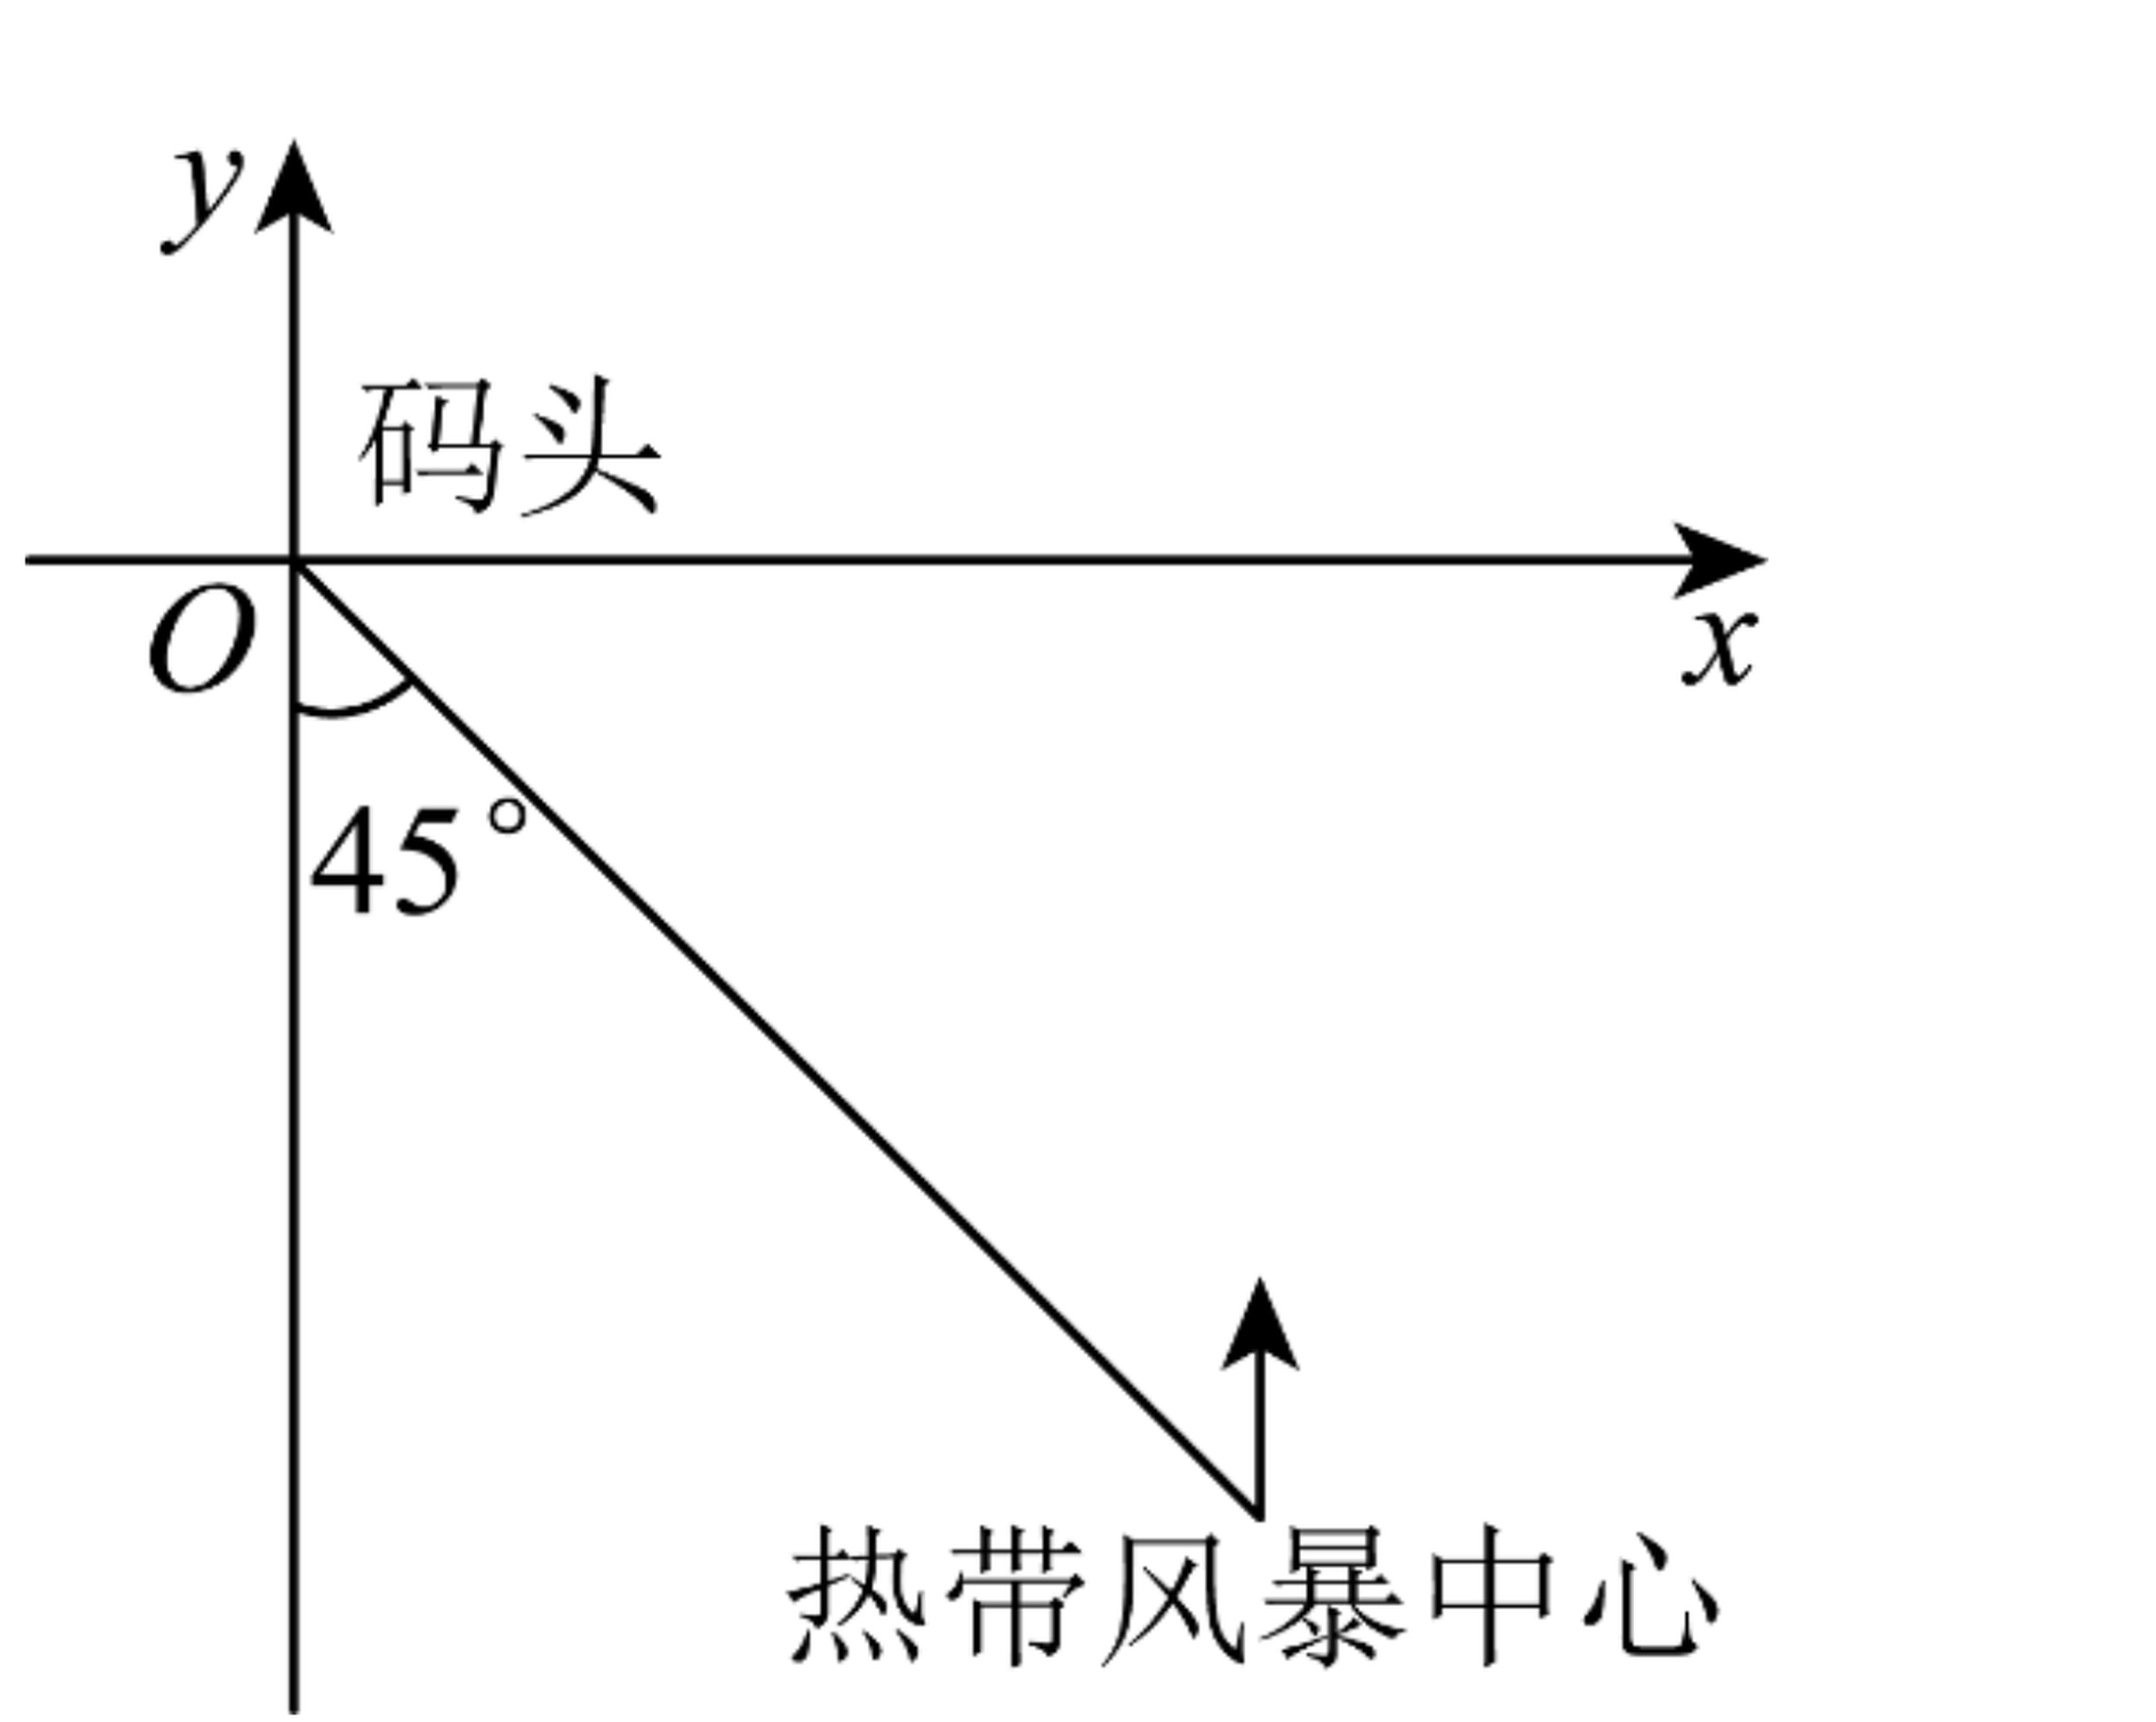
\includegraphics[width=0.36\textwidth]{figures/gao123_q5.png}
\end{center}

\ifanswer
\solbegin
\step{设风暴中心的坐标为 $(a,b)$，}
\step{由题意得 $a=400\sqrt2\times\cos45^\circ=400$，当 $a^2+b^2=400^2+b^2<500^2$，}% 原卷 $a^2$ 与 $400^2$ 并用，照录
\step{即 $-300<b<300$ 时，码头将受到风暴影响，}
\step{$\dfrac{300-(-300)}{20}=30h$，则码头受到风暴影响的时长为 30 小时，}
\step{所以由预报估计，该码头将受到热带风暴的影响时长大约为 30 小时.}
\solend
\fi

\item 已知 $a$、$b$、$c$ 为常数，若不等式 $\dfrac{ax-b}{x-c}\geqslant0$ 的解集为 $[-1,1)$，则不等式 $ax+b<0$ 的解集为\blankline[4.4em].

\ifanswer
\solbegin
\step{不等式 $\dfrac{ax-b}{x-c}\geqslant0$ 可化为 $(ax-b)(x-c)\geqslant0$ 且 $x-c\neq0$，}
\step{即 $a\left(x-\dfrac ba\right)(x-c)\geqslant0$ 且 $x\neq c$，}
\step{因为不等式 $\dfrac{ax-b}{x-c}\geqslant0$ 的解集为 $[-1,1)$，所以 $a<0$，且 $\dfrac ba=-1$,$c=1$，}
\step{即 $b=-a$，所以不等式 $ax+b<0$ 可化为 $ax-a<0$，又因为 $a<0$，所以 $x-1>0$，}
\step{解得 $x>1$，所以不等式 $ax+b<0$ 的解集为 $(1,+\infty)$.}
\solend
\fi

\item 已知实数 $a$、$b$ 满足 $ab=32$，且 $\log_2a=\log_b16$，则 $a+b$ 的值为\blankline[4.4em].

\ifanswer
\solbegin
\step{由 $\log_2a=\log_b16$，得 $\log_2a=\dfrac{\log_216}{\log_2b}$，则 $\log_2a\cdot\log_2b=4$，}
\step{由 $ab=32$，得 $\log_2a+\log_2b=\log_2ab=5$，}
\step{得 $\log_2a=1$,$\log_2b=4$ 或 $\log_2a=4$,$\log_2b=1$，}
\step{因此 $a=2$,$b=16$ 或 $a=16$,$b=2$，所以 $a+b=18$.}
\solend
\fi

\item 已知实数 $a$、$b$ 满足 $-3<a+2b<2$，$-1<2a-b<4$，则 $a+b$ 的取值范围为\blankline[4.4em].

\ifanswer
\solbegin
\step{设 $a+b=m(a+2b)+n(2a-b)=(m+2n)a+(2m-n)b$，}
\step{所以 $\begin{cases}m+2n=1\\2m-n=1\end{cases}$，解得 $n=\dfrac15$,$m=\dfrac35$，所以 $a+b=\dfrac35(a+2b)+\dfrac15(2a-b)$，}
\step{因为 $-3<(a+2b)<2$，$-1<2a-b<4$，}
\step{所以 $-\dfrac95<\dfrac35(a+2b)<\dfrac65$，$-\dfrac15<\dfrac15(2a-b)<\dfrac45$，}
\step{相加得 $-2<\dfrac35(a+2b)+\dfrac15(2a-b)<2$，即 $-2<a+b<2$，}
\step{故 $a+b$ 的取值范围为 $(-2,2)$.}
\solend
\fi

\item 存在 $x\in\R$ 使不等式 $\lvert2x-a\rvert<\lvert2a-1\rvert-2\lvert x\rvert$ 成立，则实数 $a$ 的取值范围是\blankline[4.4em].

\ifanswer
\solbegin
\step{存在 $x\in\R$，不等式 $\lvert2x-a\rvert<\lvert2a-1\rvert-2\lvert x\rvert$ 成立，}
\step{变形即 $\lvert2x-a\rvert+2\lvert x\rvert<\lvert2a-1\rvert$ 成立，}
\step{由于 $\lvert2x-a\rvert+\lvert2x\rvert\geqslant\lvert(2x-a)-2x\rvert=\lvert a\rvert$，当且仅当 $2x(2x-a)\leqslant0$ 时取等号，}
\step{因此有 $\lvert a\rvert<\lvert2a-1\rvert$，两边平方 $a^2<(2a-1)^2$，解得 $a>1$ 得 $a<\dfrac13$，}% 原卷“解得 a>1 得 a<1/3”，照录
\step{即实数 $a$ 的取值范围是 $\left(-\infty,\dfrac13\right)\cup(1,+\infty)$.}
\solend
\fi

\item 已知集合 $A=\{(x,y)\mid x^2+mx-y+2=0\}$，$B=\{(x,y)\mid x-y+1=0,0\leqslant x\leqslant3\}$，若集合 $A\cap B$ 的子集个数为 $2$，则实数 $m$ 的取值范围为\blankline[4.4em].

\ifanswer
\solbegin
\step{因为集合 $A\cap B$ 的子集个数为 $2$，所以 $A\cap B$ 的元素有一个，}
\step{即 $\begin{cases}x^2+mx-y+2=0\\x-y+1=0\end{cases}$ 在 $x\in[0,3]$ 上只有一个解，}
\step{即 $x^2+(m-1)x+1=0$ 在 $[0,3]$ 上只有一个解，}
\step{即 $1-m=x+\dfrac1x$ 在 $[0,3]$ 上只有一个解，}
\step{结合对勾函数的性质得 $1-m=2$ 或 $1-m>\dfrac{10}{3}$，解得 $m=-1$ 或 $m<-\dfrac73$.}
\solend
\fi

\item $[x]$ 表示不超过 $x$ 的最大整数，则集合 $A=\left\{y\,\middle\vert\,y=\left[\dfrac{x^2}{100}\right],x=1,2,3,\cdots,100\right\}$ 中的元素个数为\blankline[4.4em].

\ifanswer
\solbegin
\step{记 $a_k=\left[\dfrac{k^2}{100}\right](k=1,2,\cdots,100)$，$a_k$ 随 $k$ 增大而单调不减.}
\step{当 $k\geqslant50$ 时，$\dfrac{(k+1)^2}{100}-\dfrac{k^2}{100}=\dfrac{2k+1}{100}\geqslant\dfrac{101}{100}>1$，所以 $a_{k+1}\geqslant a_k+1$，}
\step{即 $a_{50}$、$a_{51}$、$\cdots$、$a_{100}$ 两两互异.}
\step{又 $a_{50}=\left[\dfrac{2500}{100}\right]=25$、$a_{100}=100$，这一段共 $100-50+1=51$ 个互异的值，}
\step{且都大于等于 $25$.}
\step{当 $k\leqslant49$ 时，$\dfrac{(k+1)^2}{100}-\dfrac{k^2}{100}=\dfrac{2k+1}{100}\leqslant\dfrac{99}{100}<1$，即 $a_k$ 每次至多增加 $1$；}
\step{又 $a_1=0$、$a_{49}=\left[\dfrac{2401}{100}\right]=24$，}
\step{故 $a_1$、$a_2$、$\cdots$、$a_{49}$ 依次取遍 $0$，$1$，$2$，$\cdots$，$24$，共 $25$ 个值.}
\step{两段取值范围互不重叠（前段不超过 $24$、后段不小于 $25$），}
\step{所以集合 $A$ 中共有 $25+51=76$ 个元素.}
\solend
\fi

\item 若实数 $a$、$b$、$c$ 满足 $\dfrac1{2^a}+\dfrac1{2^b}=1$，$\dfrac1{2^{a+b}}+\dfrac1{2^{b+c}}+\dfrac1{2^{a+c}}=1$，则 $c$ 的最大值是\blankline[4.4em].

\ifanswer
\solbegin
\step{因为 $\dfrac1{2^a}+\dfrac1{2^b}=1$，}
\step{由基本不等式得 $1=\dfrac1{2^a}+\dfrac1{2^b}\geqslant2\sqrt{\dfrac1{2^a}\cdot\dfrac1{2^b}}$（当且仅当 $a=b=1$ 时取等号），}
\step{所以 $\dfrac1{2^a}\cdot\dfrac1{2^b}\leqslant\dfrac14$，所以 $-\dfrac1{2^a}\cdot\dfrac1{2^b}\geqslant-\dfrac14$，}% 原卷带负号起论，照录
\step{因为 $\dfrac1{2^{a+b}}+\dfrac1{2^{b+c}}+\dfrac1{2^{a+c}}=1$，$\dfrac1{2^{b+c}}+\dfrac1{2^{a+c}}=\dfrac1{2^c}\left(\dfrac1{2^a}+\dfrac1{2^b}\right)=\dfrac1{2^c}$，}
\step{所以 $\dfrac1{2^c}=1-\dfrac1{2^{a+b}}\geqslant\dfrac34$，所以 $2^c\leqslant\dfrac43$，所以 $c\leqslant\log_2\dfrac43=2-\log_23$，}
\step{故 $c$ 的最大值是 $2-\log_23$.}
\solend
\fi

\end{enumerate}

\bigsec{二、选择题}

\begin{enumerate}
\setcounter{enumi}{12}

\item 下列运用等式或不等式的性质变形中，正确的是\mbox{（\quad）}

\keepwithprev
A. 如果 $a=b$，那么 $\dfrac ac=\dfrac bc$\qquad\qquad B. 如果 $\dfrac1a<\dfrac1b<0$，那么 $a-\dfrac1a>b-\dfrac1b$

C. 如果 $a>b$，那么 $\dfrac1a<\dfrac1b$\qquad\qquad D. 如果 $a>b>0$，$m\in\R$，那么 $\dfrac ba<\dfrac{b+m}{a+m}$

\ifanswer
\solbegin
\step{对于 $A$，若 $c=0$，$A$ 错误；}
\step{对于 $B$，若 $\dfrac1a<\dfrac1b<0$，则 $0>a>b$，$-\dfrac1a>-\dfrac1b>0$，}
\step{所以 $a-\dfrac1a>b-\dfrac1b$，$B$ 正确；}
\step{对于 $C$，$a>0$，$b<0$ 时，$C$ 错误；}
\step{对于 $D$，$\dfrac{b+m}{a+m}-\dfrac ba=\dfrac{ab+am}{a(a+m)}-\dfrac{ab+bm}{a(a+m)}=\dfrac{(a-b)m}{a(a+m)}$，}
\step{因为 $a>b>0$，所以 $a-b>0$，但 $m$、$a+m$ 的符号不确定，}
\step{当 $m=0$ 时，$\dfrac ba=\dfrac{b+m}{a+m}$，}
\step{当 $m(a+m)>0$ 时，$\dfrac ba<\dfrac{b+m}{a+m}$，当 $m(a+m)<0$ 时，$\dfrac ba>\dfrac{b+m}{a+m}$，$D$ 错误.}
\step{故选 $B$.}
\solend
\fi

\item “$a>b$”的一个必要非充分条件是\mbox{（\quad）}

\keepwithprev
A. $ac^2>bc^2$\qquad\quad B. $2^a>2^b$\qquad\quad C. $\left(\dfrac12\right)^{a-b}\leqslant1$\qquad\quad D. $a^3>b^3$

\ifanswer
\solbegin
\step{即“$a>b$”能推出选项，但选项不能推出“$a>b$”，故选 $C$.}
\solend
\fi

\item 若 $A=\left\{x\,\middle\vert\,x=\dfrac k6+1,k\in\Z\right\}$，$B=\left\{x\,\middle\vert\,x=\dfrac k3+\dfrac12,k\in\Z\right\}$，$C=\left\{x\,\middle\vert\,x=\dfrac{2k}{3}+\dfrac12,k\in\Z\right\}$，则这三个集合间的关系是\mbox{（\quad）}

\keepwithprev
A. $A\subseteq B\subseteq C$\qquad\quad B. $A\subseteq C\subseteq B$\qquad\quad C. $C\subseteq B\subseteq A$\qquad\quad D. $C\subseteq A\subseteq B$

\ifanswer
\solbegin
\step{若 $x\in C$，则存在 $k_0\in\Z$，使 $x=\dfrac{2k_0}{3}+\dfrac12$，}
\step{又 $2k_0\in\Z$，所以 $x\in B$，故 $C\subseteq B$，}
\step{若 $x\in B$，则存在 $k_1\in\Z$，使 $x=\dfrac{k_1}{3}+\dfrac12=\dfrac{2k_1-3}{6}+1$，}
\step{又 $2k_1-3\in\Z$，所以 $x\in A$，故 $B\subseteq A$，}
\step{又 $\dfrac43\in A$，$\dfrac43\notin B$，$\dfrac56\in B$，$\dfrac56\notin C$，所以 $C\subseteq B\subseteq A$，故选 $C$.}
\solend
\fi

\item 集合 $S=\{x\mid(x+a)(x^2+bx+c)=0\}$，$T=\{x\mid(ax+1)(cx^2+bx+1)=0\}$，其中 $a$、$b$、$c$ 为实数，若 $\lvert S\rvert$、$\lvert T\rvert$ 分别表示 $S$、$T$ 的元素个数，则下列结论中一定成立的是\mbox{（\quad）}

\keepwithprev
A. 若 $\lvert T\rvert=0$，则 $\lvert S\rvert=1$\qquad\qquad B. 若 $\lvert S\rvert=1$，则 $\lvert T\rvert=1$

C. 若 $\lvert S\rvert=2$，则 $\lvert T\rvert=2$\qquad\qquad D. 若 $\lvert T\rvert=3$，则 $\lvert S\rvert=2$

\ifanswer
\solbegin
\step{令 $f(x)=(x+a)(x^2+bx+c)$,$g(x)=(ax+1)(cx^2+bx+1)$，}
\step{对于选项 A，当 $\lvert T\rvert=0$ 时，方程 $g(x)=(ax+1)(cx^2+bx+1)=0$ 无实根，}
\step{当 $a=b=c=0$ 时，$f(x)=x^3$，由 $f(x)=0$ 得 $x=0$，此时 $\lvert S\rvert=1$；}
\step{当 $a=0$,$b^2-4c<0$ 时，$f(x)=x(x^2+bx+c)$，由 $f(x)=0$ 得 $x=0$，}
\step{此时 $\lvert S\rvert=1$，所以选项 A 正确；}
\step{对于选项 B，若 $\lvert S\rvert=1$，则 $f(x)=(x+a)(x^2+bx+c)=0$ 有且只有一根，}
\step{又 $x=-a$ 一定是 $f(x)=0$ 的根，所以 $\triangle=b^2-4c<0$，}
\step{又 $\triangle=b^2-4c<0$ 且 $a=0$ 时，$g(x)=(ax+1)(cx^2+bx+1)=0$ 无解，}
\step{此时 $\lvert T\rvert=0$，所以选项 B 错误，}
\step{对于选项 C，若 $\lvert S\rvert=2$ 时，则 $f(x)=(x+a)(x^2+bx+c)=0$ 有且只有 $2$ 根，}
\step{又 $x=-a$ 一定是 $f(x)=0$ 的根，}
\step{所以 $\triangle=b^2-4c=0$ 且 $a^2+ab+c\neq0$ 或 $\triangle=b^2-4c>0$ 且 $a^2+ab+c=0$，}
\step{当 $a=0$ 时，存在 $b$,$c$，使 $\triangle=b^2-4c=0$ 且 $a^2+ab+c\neq0$，}
\step{此时 $g(x)=(ax+1)(cx^2+bx+1)=0$ 只有一根，所以选项 C 错误，}
\step{对于选项 D，当 $\lvert T\rvert=3$ 时，方程 $g(x)=(ax+1)(cx^2+bx+1)=0$ 有三个根，}
\step{所以 $a\neq0$,$c\neq0$,$b^2-4c>0$，}
\step{设 $x_0$ 为 $g(x)=0$ 的一个根，即 $(ax_0+1)(cx_0^2+bx_0+1)=0$，}
\step{则 $x_0\neq0$，且 $f\left(\dfrac1{x_0}\right)=\left(\dfrac1{x_0}+a\right)\left(\dfrac1{x_0^2}+\dfrac1{x_0}b+c\right)=\dfrac1{x_0^3}g(x_0)=0$，}
\step{所以 $\dfrac1{x_0}$ 为方程 $f(x)=0$ 的根，故 $f(x)=0$ 有三个根，即 $\lvert T\rvert=3$ 时，}
\step{必有 $\lvert S\rvert=3$，所以选项 D 错误，}
\step{故选 $A$.}
\solend
\fi

\end{enumerate}

% 第 17 题是解答题第一题且带文氏图，守卫放在 \bigsec 之前，连节标题一起量页高
\needvspace{7cm}
\bigsec{三、解答题}

\begin{enumerate}
\setcounter{enumi}{16}

\item 设全集 $U=\R$，集合 $A=\{x\mid-2\leqslant x\leqslant4\}$，$B=\{x\mid x<-6$ 或 $x\geqslant2\}$.

（1）求图中阴影部分表示的集合；

（2）已知集合 $C=\{x\mid10-a<x<2a+1\}$，若 $\overline B\cap C=\varnothing$，求 $a$ 的取值范围.

\begin{center}
% 图取原卷截图（第 7 页题干右侧）、去水印后 2× LANCZOS 放大，本稿移至题干之后
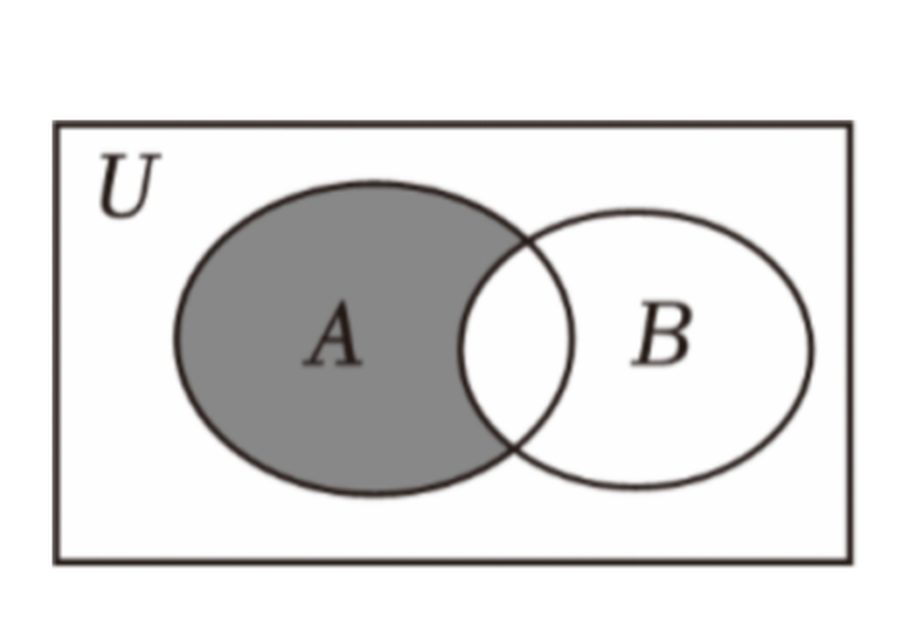
\includegraphics[width=0.34\textwidth]{figures/gao123_q17.png}
\end{center}

\ifanswer
\solbegin
\step{（1）$A\cap B=\{x\mid2\leqslant x\leqslant4\}$，}
\step{则图中阴影部分表示 $\overline{A\cap B}=\{x\mid-2\leqslant x<2\}$.}% 原卷把上划线盖在整个 $A\cap B$ 上，照录
\step{（2）由题意得 $\overline B=\{x\mid-6\leqslant x<2\}$，$C\subseteq B$，}
\step{所以当 $C=\varnothing$ 时，$10-a\geqslant2a+1$，解得 $a\leqslant3$，符合题意；}
\step{当 $C\neq\varnothing$ 时，$\begin{cases}10-a<2a+1\\2a+1\leqslant-6\end{cases}$ 或者 $\begin{cases}10-a<2a+1\\10-a\geqslant2\end{cases}$，}
\step{此时不等式组 $\begin{cases}10-a<2a+1\\2a+1\leqslant-6\end{cases}$ 无解，}
\step{不等式组 $\begin{cases}10-a<2a+1\\10-a\geqslant2\end{cases}$ 的解集为 $3<a\leqslant8$，}
\step{综上，$a$ 的取值范围为 $\{a\mid a\leqslant8\}$.}
\solend
\fi

\item (1) 求不等式：$\lvert x-1\rvert+\lvert x-2\rvert\leqslant5$ 的解集.

(2) 当 $m<1$ 时，解关于 $x$ 的不等式 $\dfrac{m(x-3)}{x+2}>1$.

\ifanswer
\solbegin
\step{(1) 当 $x<1$ 时，$\lvert x-1\rvert+\lvert x-2\rvert\leqslant5\Leftrightarrow-x+1+2-x\leqslant5$，}
\step{解得 $-1\leqslant x<1$；}
\step{当 $1\leqslant x\leqslant2$ 时，$\lvert x-1\rvert+\lvert x-2\rvert\leqslant5\Leftrightarrow x-1+2-x=1\leqslant5$ 恒成立，}
\step{所以 $1\leqslant x\leqslant2$；}
\step{当 $x>2$ 时，$\lvert x-1\rvert+\lvert x-2\rvert\leqslant5\Leftrightarrow x-1+x-2=2x-3\leqslant5$，}
\step{解得 $2<x\leqslant4$.}
\step{综上所述，不等式 $\lvert x-1\rvert+\lvert x-2\rvert\leqslant5$ 的解集为 $[-1,4]$.}
\step{(2) 原不等式变成 $\dfrac{(m-1)x-(3m+2)}{x+2}>0$，$n<1$，所以 $n-1<0$，}% 原卷作 $n<1$、$n-1<0$，与题设 $m<1$ 字母不一致，照录
\step{所以原不等式变成 $\dfrac{x-\dfrac{3m+2}{m-1}}{x+2}<0$，$\dfrac{3m+2}{m-1}-(-2)=\dfrac{5m}{m-1}$，}
\step{所以 $m<0$ 时，$\dfrac{5m}{m-1}>0$，$\dfrac{3m+2}{m-1}>-2$，}
\step{原不等式的解集为 $\left(-2,\dfrac{3m+2}{m-1}\right)$；}
\step{$m=0$ 时，原不等式变成 $1<0$，无解；}
\step{$0<m<1$ 时，$\dfrac{5m}{m-1}<0$，$\dfrac{3m+2}{m-1}<-2$，}
\step{原不等式的解集为 $\left(\dfrac{3m+2}{m-1},-2\right)$.}
\solend
\fi

\item 在园林博览会上，某公司带来了一种智能设备供采购商洽谈采购，并决定大量投放市场，已知该种设备年固定研发成本为 $50$ 万元，每生产一台需另投入 $100$ 元，设该公司一年内生产该设备 $x$ 万台且全部售完，每万台的销售收入 $G(x)$（万元）与年产量 $x$（万台）满足如下关系式：$G(x)=\begin{cases}180-x,0<x\leqslant20\\80+\dfrac{2000}{x}-\dfrac{8000}{x(x-1)},x>20\end{cases}$.

(1) 写出年利润 $W(x)$（万元）关于年产量 $x$（万台）的函数解析式；（利润 $=$ 销售收入 $-$ 成本）

(2) 当年产量为多少万台时，该公司获得的年利润最大，并求出最大利润.

\ifanswer
\solbegin
\step{(1) $W(x)=xG(x)-50-100x=\begin{cases}-50+80x-x^2,0<x\leqslant20\\-20x+1950-\dfrac{8000}{x-1},x>20\end{cases}$；}
\step{(2) 当 $0<x\leqslant20$ 时，$W(x)=-50+80x-x^2=-(x-40)^2+1550$，}
\step{由函数性质得当 $x\leqslant40$ 时严格增，所以当 $x=20$ 时，$W(x)_{max}=1150$，}
\step{当 $x>20$ 时，$W(x)=-20x+1950-\dfrac{8000}{x-1}=-20\left[(x-1)+\dfrac{400}{x-1}\right]+1930$，}
\step{$W(x)=-20\left[(x-1)+\dfrac{400}{x-1}\right]+1930\leqslant-20\times2\sqrt{(x-1)\cdot\dfrac{400}{x-1}}+1930$}
\step{$=1130$，当且仅当 $x-1=\dfrac{400}{x-1}$，即 $x=21$ 时取等号，}
\step{所以 $W(x)_{max}=1130$，}
\step{因为 $1150>1130$，所以当 $x=20$ 时，$W(x)_{max}=1150$，}
\step{即当年产量为 $20$ 万台时，该公司获得的年利润最大，}
\step{最大利润为 $1150$ 万元.}
\solend
\fi

\item 关于 $x$ 的方程 $(x^2-1)^2-2k\lvert x^2-1\rvert+k+1=0(k\in\R)$.

(1) 若方程无实根，求 $k$ 的取值范围；

(2) 若方程有 $4$ 个不等实根，求 $k$ 的取值范围；

(3) 若 $k=a+b$，且满足 $\dfrac1{a+2b}+\dfrac1{a+3}=\dfrac12$，$a>0$，$b>0$，试判断方程根的个数.

\ifanswer
\solbegin
\step{(1) 关于 $x$ 的方程 $(x^2-1)^2-2k\lvert x^2-1\rvert+k+1=0(k\in\R)$，}
\step{令 $t=\lvert x^2-1\rvert$，则 $t\geqslant0$，则原方程转化为 $t^2-2kt+k+1=0(*)$，}
\step{因为关于 $x$ 的方程 $(x^2-1)^2-2k\lvert x^2-1\rvert+k+1=0(k\in\R)$ 无实根，}
\step{所以 $(*)$ 式无实根或实根均小于零，令 $f(t)=t^2-2kt+k+1$，}
\step{①若 $(*)$ 式无实根，则 $\triangle<0$，解得 $\dfrac{1-\sqrt5}{2}<k<\dfrac{1+\sqrt5}{2}$，}
\step{②两根均为负，则 $\begin{cases}\Delta\geqslant0\\t_{\text{对}}=k<0\\f(0)>0\end{cases}$，解得 $-1<k\leqslant\dfrac{1-\sqrt5}{2}$，}
\step{综合①②，得 $k$ 的取值范围是 $\left(-1,\dfrac{1+\sqrt5}{2}\right)$；}
\step{(2) 作函数 $t=\lvert x^2-1\rvert$ 的图象，}
\begin{center}
% 图取原卷截图（第 11 页解析内）、去水印后 2× LANCZOS 放大，仅答案版出
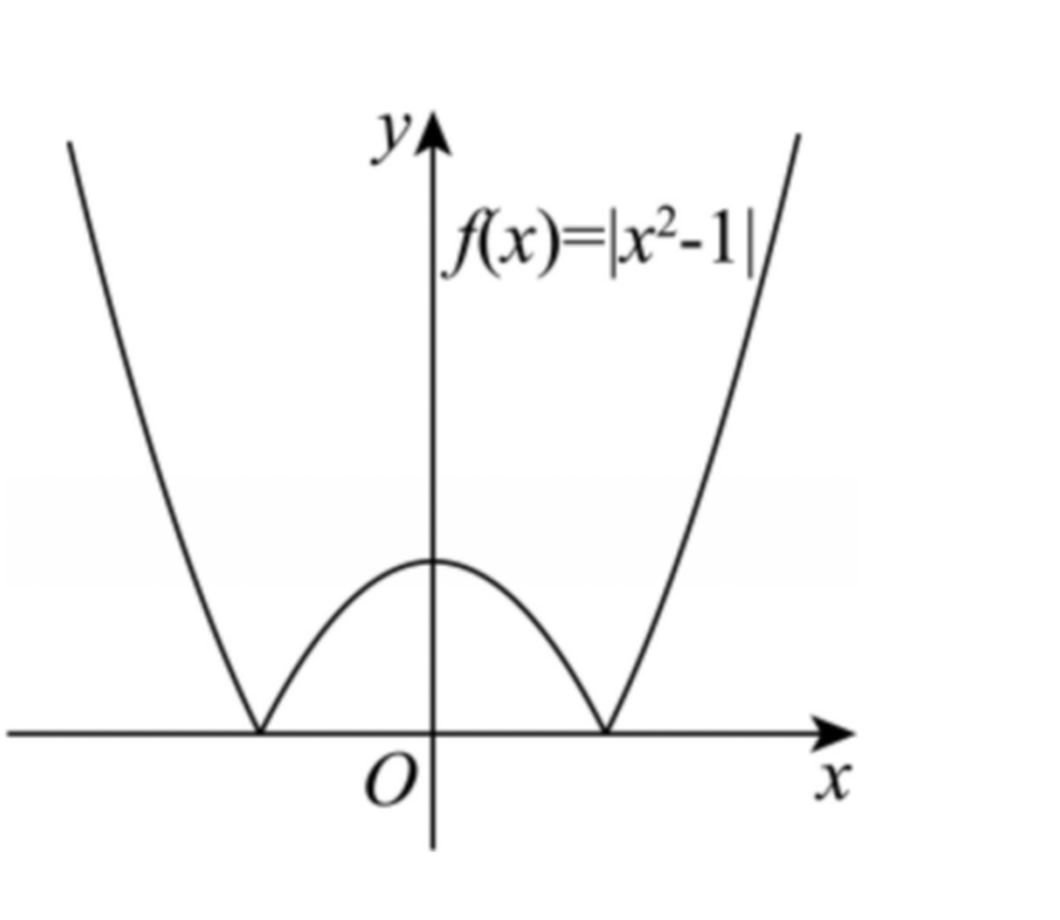
\includegraphics[width=0.40\textwidth]{figures/gao123_q20.png}
\end{center}
\step{$t=0$ 或 $t>1$ 时，每一个 $t$ 值对应 $2$ 个不同的 $x$ 值，}
\step{$t=1$ 时一个 $t$ 值对应 $3$ 个不同的 $x$ 值，}
\step{$0<t<1$ 时一个 $t$ 值对应 $4$ 个不同的 $x$ 值，}
\step{要使原方程有四个不等实根，}
\step{①$(*)$ 式一根为零，另一根大于 $1$，无解；}
\step{②$(*)$ 有两不等根且两根均大于 $1$，则 $\begin{cases}\Delta>0\\t_{\text{对}}=k>1\\f(1)>0\end{cases}$，解得 $\dfrac{1+\sqrt5}{2}<k<2$；}
\step{④$(*)$ 式有 $1$ 实根在 $(0,1)$ 之间，另一根小于零，}% 原卷由 ② 直接跳到 ④，缺 ③，照录
\step{则 $\begin{cases}f(0)<0\\f(1)>0\end{cases}$，所以 $\begin{cases}k+1<0\\2-k>0\end{cases}$，解得 $k<-1$，}
\step{综上所述，$k$ 取值范围为 $(-\infty,-1)\cup\left(\dfrac{1+\sqrt5}{2},2\right)$；}
\step{(3) 因为 $\dfrac1{a+2b}+\dfrac1{a+3}=\dfrac{a+2b+a+3}{(a+2b)(a+3)}=\dfrac{2(a+b)+3}{(a+2b)(a+3)}=\dfrac12$，}
\step{所以 $2(a+b)+3=\dfrac12(a+2b)(a+3)$，}
\step{因为 $a$、$b$ 为正实数，所以 $\dfrac12=\dfrac1{a+2b}+\dfrac1{a+3}\geqslant2\sqrt{\dfrac1{a+2b}\times\dfrac1{a+3}}$，}
\step{得 $\dfrac1{16}\geqslant\dfrac1{a+2b}\times\dfrac1{a+3}$，即 $(a+2b)(a+3)\geqslant16$，}
\step{所以 $2(a+b)+3\geqslant8$，即 $a+b\geqslant\dfrac52$，}
\step{当且仅当 $\dfrac1{a+2b}=\dfrac1{a+3}$ 即 $a=1$,$b=\dfrac32$ 时取等号，}
\step{故 $k\geqslant\dfrac52$，此时有 $\begin{cases}\Delta>0\\t_{\text{对}}=k>1\\f(0)>0,f(1)<0\end{cases}$，}
\step{故 $(*)$ 式有两不等实根且一根在 $(0,1)$ 之间，另一根大于 $1$，}
\step{故原方程有 $6$ 个实根.}
\solend
\fi

\item 设 $n$ 是不小于 $3$ 的正整数，集合 $S_n=\{(a_1,a_2,\cdots,a_n)\mid a_i\in\{0,1\},i=1,2,\cdots,n\}$，对于集合 $S_n$ 中任意两个元素 $A=(a_1,a_2,\cdots,a_n)$，$B=(b_1,b_2,\cdots,b_n)$.

定义 1：$A\cdot B=n-(\lvert a_1-b_1\rvert+\lvert a_2-b_2\rvert+\cdots+\lvert a_n-b_n\rvert)$，

定义 2：若 $A\cdot B=0$，则称互为相反元素，记作 $A=\overline B$ 或 $B=\overline A$.

(1) 若 $n=3$，$A=(0,1,0)$，$B=(1,1,0)$，试写出 $\overline A$、$\overline B$ 以及 $A\cdot B$ 的值；

(2) 若 $A$、$B\in S_n$，$A=(a_1,a_2,\cdots,a_n)$，$B=(b_1,b_2,\cdots,b_n)$，证明：$A\cdot B+\overline A\cdot B=n$；

(3) 设 $k$ 是小于 $n$ 的正奇数，至少含有两个元素的集合 $M\subseteq S_n$，且对于集合 $M$ 中任意两个不相同的元素 $A=(a_1,a_2,\cdots,a_n)$，$B=(b_1,b_2,\cdots,b_n)$，都有 $A\cdot B=n-k$，试求集合 $M$ 中元素个数的所有可能值.

\ifanswer
\solbegin
\step{(1) $\overline A=(1,0,1)$,$\overline B=(0,0,1)$,$\overline A\cdot\overline B=2$；}
\step{(2) 设 $A=(a_1,a_2,\cdots,a_n)$,$B=(b_1,b_2,\cdots,b_n)$,$\overline A=(x_1,x_2,\cdots,x_n)$，}
\step{由 $a_i$、$b_i$、$x_i\in\{0,1\}$，$i=1,2,\cdots,n$，得 $\lvert a_i-x_i\rvert\leqslant1$，$i=1,2,\cdots,n$，}
\step{所以 $\lvert a_1-x_1\rvert+\lvert a_2-x_2\rvert+\cdots+\lvert a_i-x_i\rvert\leqslant n$，}% 原卷末项下标作 $i$，照录
\step{当且仅当 $\lvert a_i-x_i\rvert=1$，$i=1,2,\cdots,n$，}
\step{即 $x_i=1-a_i$，$i=1,2,\cdots,n$ 时取等号.}
\step{由题意得 $A\cdot\overline A=n-(\lvert a_1-x_1\rvert+\lvert a_2-x_2\rvert+\cdots+\lvert a_n-x_n\rvert)=0$，}
\step{即 $\lvert a_1-x_1\rvert+\lvert a_2-x_2\rvert+\cdots+\lvert a_n-x_n\rvert=n$，}
\step{所以 $x_i=1-a_i$，$i=1,2,\cdots,n$，}
\step{$A\cdot B+\overline A\cdot B=2n-\sum\limits_{i=1}^n[\lvert a_i-b_i\rvert+(1-a_i)-b_i]$}
\step{$=2n-\sum\limits_{i=1}^n(\lvert1-b_i\rvert+\lvert0-b_i\rvert)=2n-\sum\limits_{i=1}^n(1-b_i+b_i)=2n-n=n$；}
\step{(3) 假设 $A=(a_1,a_2,\cdots,a_n)$，$B=(b_1,b_2,\cdots,b_n)$，$C=(c_1,c_2,\cdots,c_n)$}
\step{为集合 $M$ 中的三个不相同的元素，}
\step{则 $A\cdot B=n-(\lvert a_1-b_1\rvert+\lvert a_2-b_2\rvert+\cdots+\lvert a_n-b_n\rvert)=n-k$，}
\step{即 $\lvert a_1-b_1\rvert+\lvert a_2-b_2\rvert+\cdots+\lvert a_n-b_n\rvert=k$，}
\step{又由题意得 $\lvert a_i-b_i\rvert=0$ 或 $1$，$i=1,2,\cdots,n$，}
\step{$\lvert a_1-b_1\rvert$、$\lvert a_2-b_2\rvert$、$\cdots$、$\lvert a_n-b_n\rvert$ 恰有 $k$ 个 $1$，$n-k$ 个 $0$，}
\step{设其中 $k$ 个等于 $1$ 的项以此为 $a_{m_1}-b_{m_1}$,$a_{m_2}-b_{m_2}$,$\cdots$,$a_{m_k}-b_{m_k}$，}
\step{$n-k$ 个等于 $0$ 的项为 $a_{m_{k+1}}-b_{m_{k+1}}$,$a_{m_{k+2}}-b_{m_{k+2}}$,$\cdots$,$a_{m_n}-b_{m_n}$，}
\step{由题意得 $A\cdot C=n-(\lvert a_1-c_1\rvert+\lvert a_2-c_2\rvert+\cdots+\lvert a_n-c_n\rvert)=n-k$，}
\step{所以 $\sum\limits_{i=1}^k\lvert a_{m_i}-c_{m_i}\rvert+\sum\limits_{j=k+1}^n\lvert a_{m_j}-c_{m_j}\rvert=k$ ①，}
\step{同理 $\sum\limits_{i=1}^k\lvert b_{m_i}-c_{m_i}\rvert+\sum\limits_{j=k+1}^n\lvert b_{m_j}-c_{m_j}\rvert=k$ ②，}
\step{因为 $\lvert a_{m_{k+1}}-b_{m_{k+1}}\rvert=\lvert a_{m_{k+2}}-b_{m_{k+2}}\rvert=\cdots=\lvert a_{m_n}-b_{m_n}\rvert=0$，}
\step{所以 $\sum\limits_{j=k+1}^n\lvert a_{m_j}-c_{m_j}\rvert=\sum\limits_{j=k+1}^n\lvert b_{m_j}-c_{m_j}\rvert$，}
\step{由①$-$②得 $\sum\limits_{i=1}^k(\lvert a_{m_i}-c_{m_i}\rvert-\lvert b_{m_i}-c_{m_i}\rvert)=0$，}
\step{又 $\sum\limits_{i=1}^k(\lvert a_{m_i}-c_{m_i}\rvert-\lvert b_{m_i}-c_{m_i}\rvert)=\sum\limits_{i=1}^k(\lvert1-c_{m_i}\rvert-\lvert0-c_{m_i}\rvert)=k-2\sum\limits_{i=1}^k c_{m_i}$}
\step{为奇数，与 $\sum\limits_{i=1}^k(\lvert a_{m_i}-c_{m_i}\rvert-\lvert b_{m_i}-c_{m_i}\rvert)=0$ 矛盾，所以假设不成立，}
\step{即集合 $M$ 中至多有两个元素，}
\step{当 $M=\{(1,1,\cdots,1,0,0,\cdots,0),(0,0,\cdots,0)\}$ 时符合题意，}
\step{所以集合 $M$ 中元素的个数只可能是 $2$.}
\solend
\fi

\end{enumerate}

\end{document}
"
%
% 原始材料：微信公众号“魔都数学加油站”文章，作者破晓，2026-11-09 17:52 发布；
% 连载“27学年高一123”，原文标题“27学年高一123——2026-2027年上海市行知中学高一上10月月考”；
% 原文链接：https://mp.weixin.qq.com/s/GV4SWBLUJrBhMQwo22FVzg。
% 正文为 14 张 PNG 页（第 7、9、11、13、14 页 2560×3620，其余 4762×6735），
% 题目下印有【答案】或【解析】，为讲评版。
% 题目、解析均据原图转录；卷面红色水印及公众号页脚未录入。
% 全卷 3 张插图：第 5 题的坐标示意图、第 17 题的文氏图（均属题干，三版都出）、
% 第 20 题 (2) 的 $t=\lvert x^2-1\rvert$ 图象（属解析，仅答案版出）；
% 都取原卷截图去水印、2× LANCZOS 放大，见 figures/gao123_q5.png、
% figures/gao123_q17.png、figures/gao123_q20.png。
%
% 卷首标题：原卷印作“2026-2027 年行知中学高一上 10 月月考”（公众号标题中的“上海市”
% 卷面标题行没有，本稿照卷面），年份区间按全稿惯例排 en dash；原卷未印副标题，本稿按题目内容
% 标为“集合与常用逻辑用语、不等式”（与 110／111／113／116／118／120 同）。
%
% 与原卷的排版差异：
%   ① 原文从第 3 题起，填空题编号为 3—12、选择题为 13—16、解答题为 17—21，本稿保留原题号；
%   ② 原卷每题下直接印【解析】／【答案】，本稿按全稿惯例置于答案版；第 3 题只印【答案】、
%      另提 \ans{}；选择题答案在解析末句“故选 …”，括号内留空；
%   ③ 原卷未印副标题，本稿按“知识模块”口径补出；
%   ④ 原卷填空横线按全稿惯例排为 \blankline[4.4em]；选择题括号排 \mbox{（\quad）}、
%      选项段前按惯例加 \keepwithprev；解答题不留作答区（原卷为讲评版，与 109—122 同）；
%   ⑤ 原卷数集排斜体 $R$／$Z$（第 9 题作粗体 $\mathbf{R}$），按全稿惯例改 \R／\Z；
%      绝对值按全稿惯例排 \lvert…\rvert，集合描述竖线排 \mid；单位 km、h 原卷排斜体，
%      本稿按正体照排；补集照原卷上划线排 \overline{B}、\overline{A}。
%
% 判别式与子集符号：第 16 题解析的 $\triangle=b^2-4c<0$、第 20 题 (1) ① 的 $\triangle<0$
%   均作等边、扁的 \triangle；第 20 题 ② 两处 cases 与 (3) 的 $\Delta\geqslant0$／$\Delta>0$
%   作等腰、高的 \Delta，逐处照录、不统一；第 15 题选项与第 17 题 (2) 的 $\subseteq$
%   印有下划线，照录 \subseteq。
%
% 原卷存疑照录：
%   第 4 题解析“若 $-\lvert a\rvert=0$，则 $a=0$，则 $A=\{0,-1,0\}$”以元素重复说明互异性；
%   第 5 题解析“当 $a^2+b^2=400^2+b^2<500^2$”等式左边 $a^2$ 与 $400^2$ 并用；
%   第 9 题解析“解得 $a>1$ 得 $a<\dfrac13$”（按平方不等式应为 $a>1$ 或 $a<\dfrac13$）；
%   第 12 题解析“所以 $-\dfrac1{2^a}\cdot\dfrac1{2^b}\geqslant-\dfrac14$”带负号起论；
%   第 17 题 (1) 解析把阴影部分（实为 $A\cap\overline B$）印作 $\overline{A\cap B}$；
%   第 18 题 (2) 解析作“$n<1$，所以 $n-1<0$”，与题设 $m<1$ 字母不一致；
%   第 20 题 (2) 的情形编号由 ①、② 直接跳到 ④（缺 ③）；
%   第 21 题 (2) 解析“$\lvert a_1-x_1\rvert+\cdots+\lvert a_i-x_i\rvert\leqslant n$”
%   末项下标作 $i$（按上下文应为 $n$）。以上均照录加注。
%
% 行数核对：逐题数 \step 条数，合计 176 条（Q3：0；Q4：6；Q5：5；Q6：5；Q7：4；
% Q8：6；Q9：5；Q10：5；Q11：10；Q12：6；Q13：9；Q14：1；Q15：5；Q16：21；
% Q17：8；Q18：14；Q19：10；Q20：26；Q21：30），与原卷印刷行逐题相等
% （cases 块作一个印刷行计）。第 3 题只印【答案】，提 \ans{}，不计入 \step 账。
%
\documentclass[a4paper,11pt]{article}
\usepackage{common}

\begin{document}

\examtitlest[3]{2026--2027 年行知中学高一上 10 月月考}{集合与常用逻辑用语、不等式}

\bigsec{一、填空题}

\begin{enumerate}
\setcounter{enumi}{2}

\item 写出命题“存在实数 $x$、$y$、$z$，使 $x<y$ 或 $y<z$.”的否定\blankline[4.4em].

\ifanswer
\ans{任意实数 $x$、$y$、$z$，使得 $x\geqslant y$ 且 $y\geqslant z$}
\fi

\item 若集合 $\{0,-1,2a\}=\{a-1,-\lvert a\rvert,a+1\}$，实数 $a$ 的值为\blankline[4.4em].

\ifanswer
\solbegin
\step{令 $A=\{0,-1,2a\}$,$B=\{a-1,-\lvert a\rvert,a+1\}$，}
\step{因为 $\{0,-1,2a\}=\{a-1,-\lvert a\rvert,a+1\}$，}
\step{若 $a-1=0$，则 $a=1$，则 $A=\{0,-1,2\}$,$B=\{0,-1,2\}$，满足要求；}
\step{若 $-\lvert a\rvert=0$，则 $a=0$，则 $A=\{0,-1,0\}$，不满足集合元素的互异性；}% 原卷以 $A=\{0,-1,0\}$ 说明互异性，照录
\step{若 $a+1=0$，则 $a=-1$，则 $A=\{0,-1,-2\}$,$B=\{0,-1,-2\}$，满足要求；}
\step{故实数 $a$ 的值为 $\pm1$.}
\solend
\fi

\needvspace{7cm}
\item 如图，据气象部门预报，在距离某码头南偏东 $45^\circ$ 方向 $400\sqrt2$ km 处的热带
风暴中心正在以 $20$km/h 的速度向正北方向移动，距风暴中心 $500$km 以内
的地区都将受到影响. 以上预报估计，该码头将受到热带风暴的影响时长大
约为\blankline[4.4em]$h$.

\begin{center}
% 图取原卷截图（第 1 页题干右侧）、去水印后 2× LANCZOS 放大，本稿移至题干之后
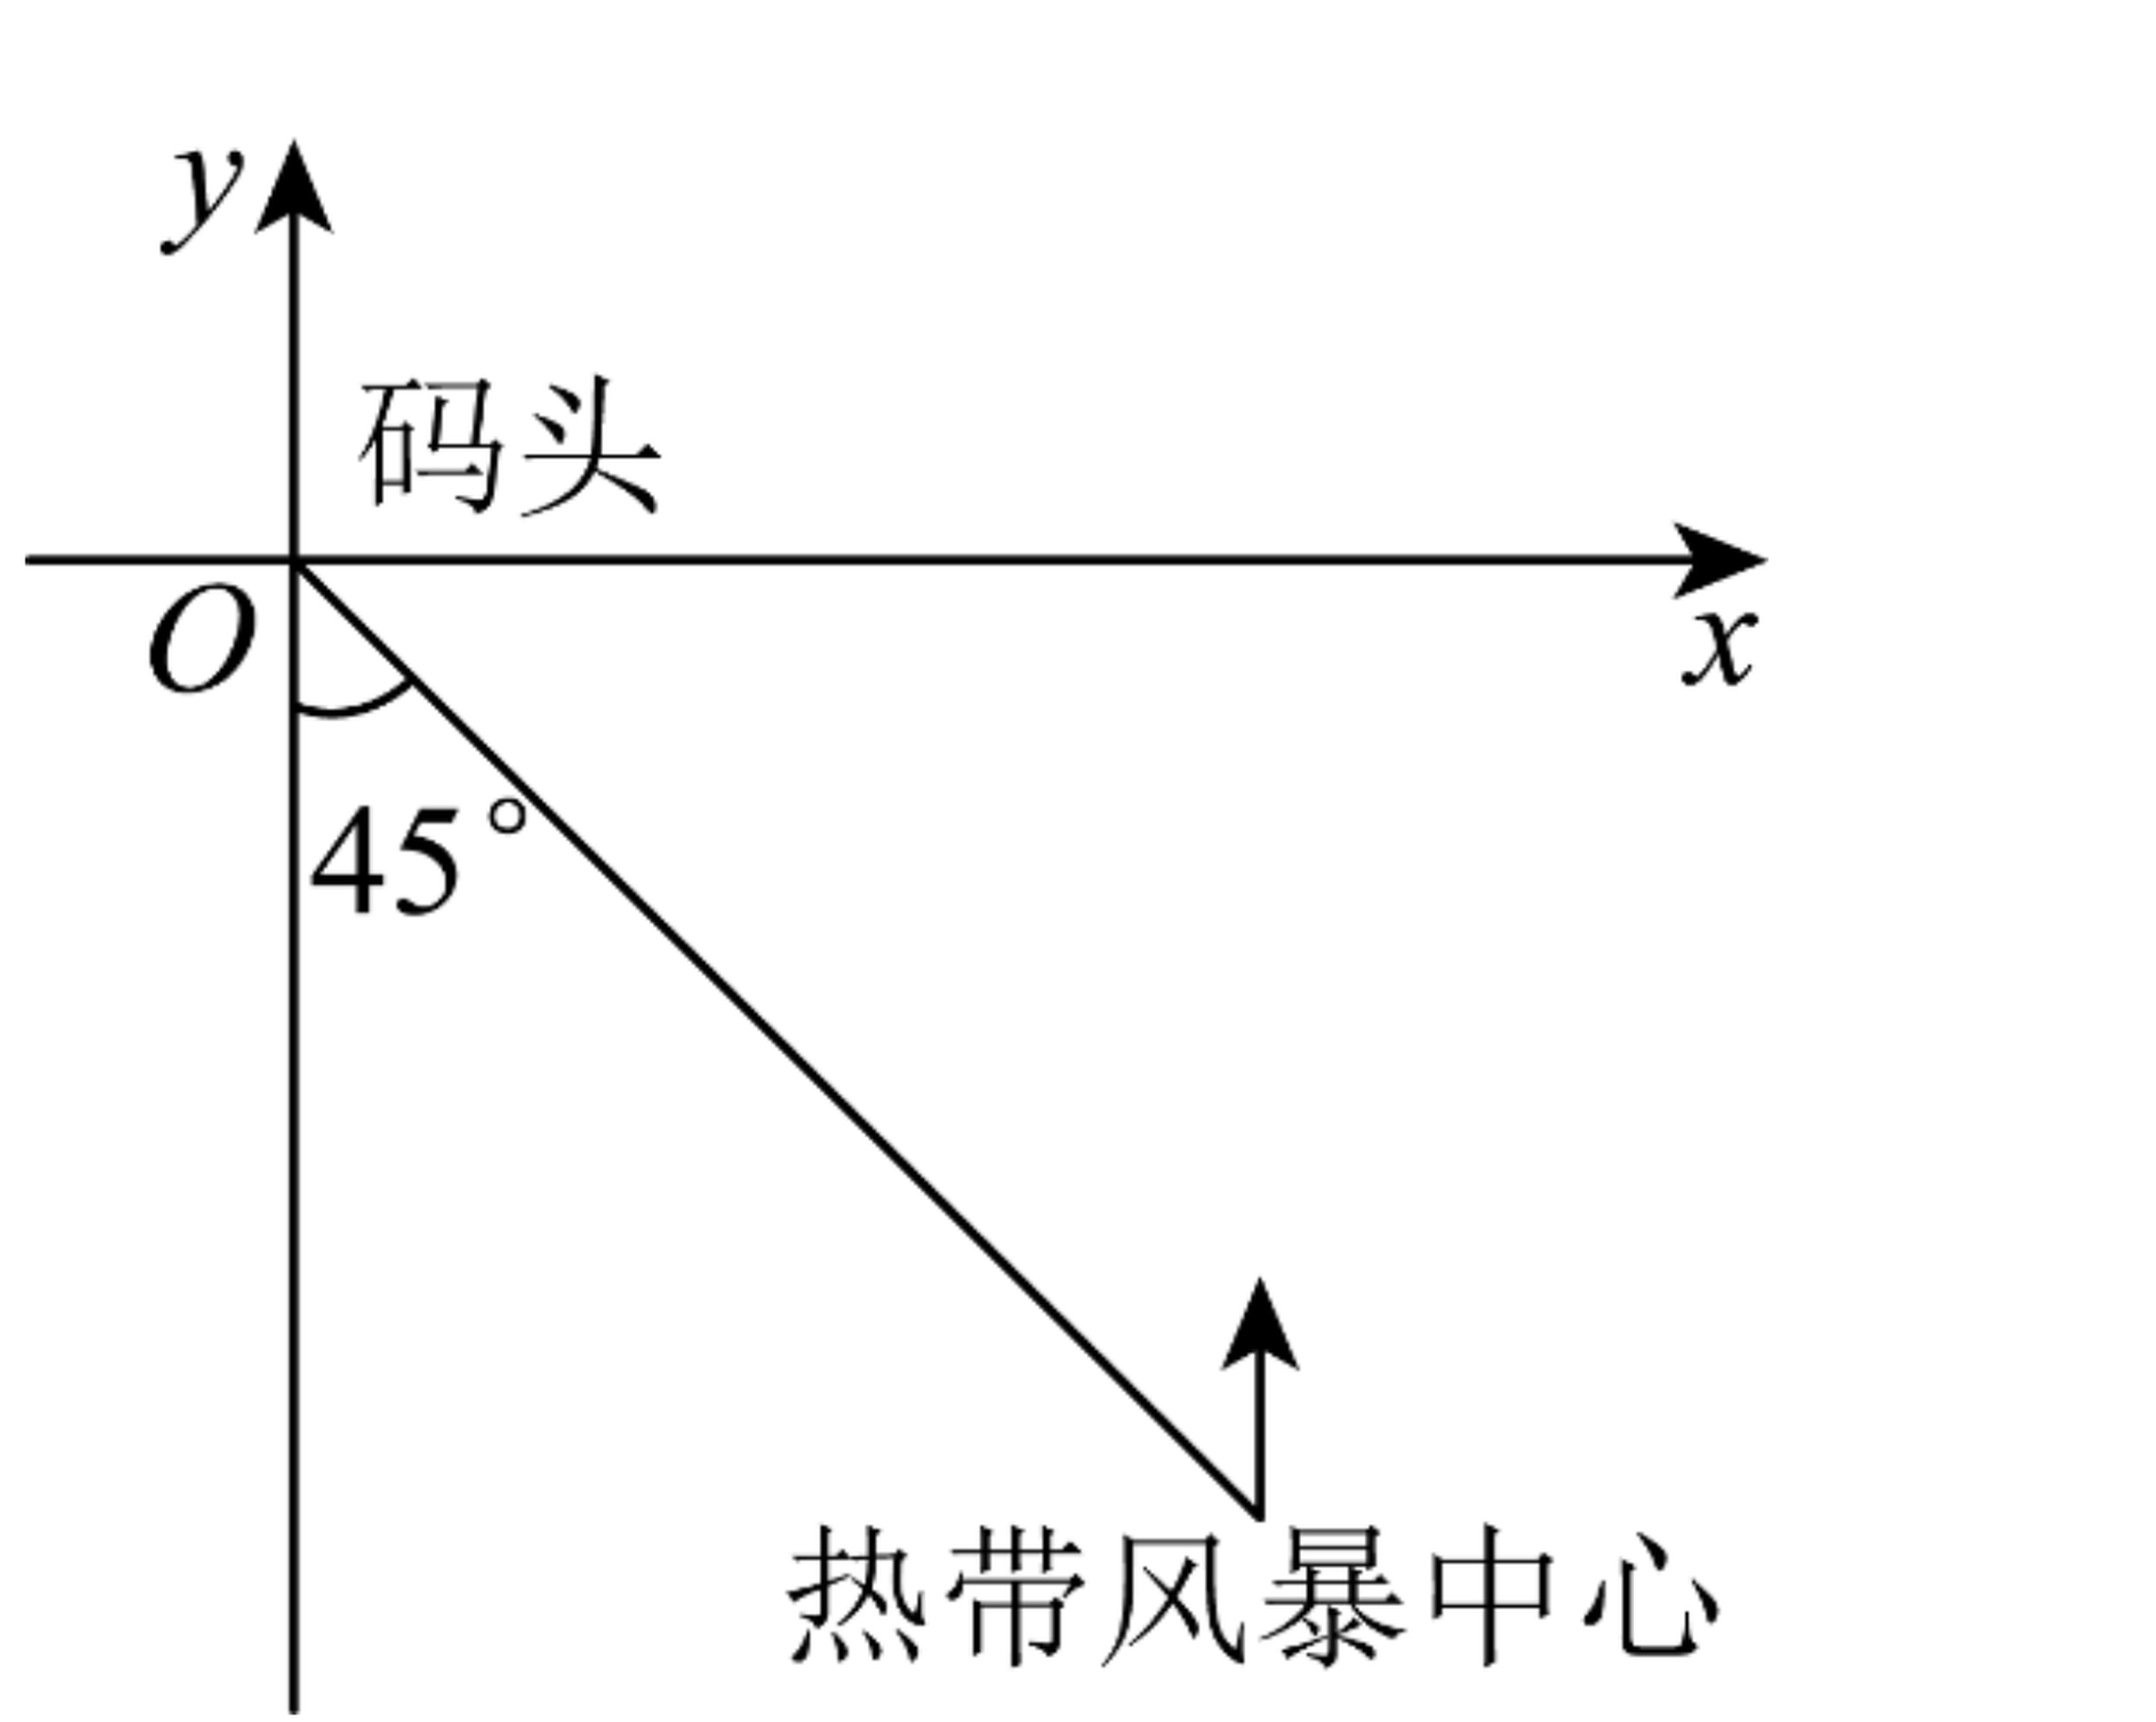
\includegraphics[width=0.36\textwidth]{figures/gao123_q5.png}
\end{center}

\ifanswer
\solbegin
\step{设风暴中心的坐标为 $(a,b)$，}
\step{由题意得 $a=400\sqrt2\times\cos45^\circ=400$，当 $a^2+b^2=400^2+b^2<500^2$，}% 原卷 $a^2$ 与 $400^2$ 并用，照录
\step{即 $-300<b<300$ 时，码头将受到风暴影响，}
\step{$\dfrac{300-(-300)}{20}=30h$，则码头受到风暴影响的时长为 30 小时，}
\step{所以由预报估计，该码头将受到热带风暴的影响时长大约为 30 小时.}
\solend
\fi

\item 已知 $a$、$b$、$c$ 为常数，若不等式 $\dfrac{ax-b}{x-c}\geqslant0$ 的解集为 $[-1,1)$，则不等式 $ax+b<0$ 的解集为\blankline[4.4em].

\ifanswer
\solbegin
\step{不等式 $\dfrac{ax-b}{x-c}\geqslant0$ 可化为 $(ax-b)(x-c)\geqslant0$ 且 $x-c\neq0$，}
\step{即 $a\left(x-\dfrac ba\right)(x-c)\geqslant0$ 且 $x\neq c$，}
\step{因为不等式 $\dfrac{ax-b}{x-c}\geqslant0$ 的解集为 $[-1,1)$，所以 $a<0$，且 $\dfrac ba=-1$,$c=1$，}
\step{即 $b=-a$，所以不等式 $ax+b<0$ 可化为 $ax-a<0$，又因为 $a<0$，所以 $x-1>0$，}
\step{解得 $x>1$，所以不等式 $ax+b<0$ 的解集为 $(1,+\infty)$.}
\solend
\fi

\item 已知实数 $a$、$b$ 满足 $ab=32$，且 $\log_2a=\log_b16$，则 $a+b$ 的值为\blankline[4.4em].

\ifanswer
\solbegin
\step{由 $\log_2a=\log_b16$，得 $\log_2a=\dfrac{\log_216}{\log_2b}$，则 $\log_2a\cdot\log_2b=4$，}
\step{由 $ab=32$，得 $\log_2a+\log_2b=\log_2ab=5$，}
\step{得 $\log_2a=1$,$\log_2b=4$ 或 $\log_2a=4$,$\log_2b=1$，}
\step{因此 $a=2$,$b=16$ 或 $a=16$,$b=2$，所以 $a+b=18$.}
\solend
\fi

\item 已知实数 $a$、$b$ 满足 $-3<a+2b<2$，$-1<2a-b<4$，则 $a+b$ 的取值范围为\blankline[4.4em].

\ifanswer
\solbegin
\step{设 $a+b=m(a+2b)+n(2a-b)=(m+2n)a+(2m-n)b$，}
\step{所以 $\begin{cases}m+2n=1\\2m-n=1\end{cases}$，解得 $n=\dfrac15$,$m=\dfrac35$，所以 $a+b=\dfrac35(a+2b)+\dfrac15(2a-b)$，}
\step{因为 $-3<(a+2b)<2$，$-1<2a-b<4$，}
\step{所以 $-\dfrac95<\dfrac35(a+2b)<\dfrac65$，$-\dfrac15<\dfrac15(2a-b)<\dfrac45$，}
\step{相加得 $-2<\dfrac35(a+2b)+\dfrac15(2a-b)<2$，即 $-2<a+b<2$，}
\step{故 $a+b$ 的取值范围为 $(-2,2)$.}
\solend
\fi

\item 存在 $x\in\R$ 使不等式 $\lvert2x-a\rvert<\lvert2a-1\rvert-2\lvert x\rvert$ 成立，则实数 $a$ 的取值范围是\blankline[4.4em].

\ifanswer
\solbegin
\step{存在 $x\in\R$，不等式 $\lvert2x-a\rvert<\lvert2a-1\rvert-2\lvert x\rvert$ 成立，}
\step{变形即 $\lvert2x-a\rvert+2\lvert x\rvert<\lvert2a-1\rvert$ 成立，}
\step{由于 $\lvert2x-a\rvert+\lvert2x\rvert\geqslant\lvert(2x-a)-2x\rvert=\lvert a\rvert$，当且仅当 $2x(2x-a)\leqslant0$ 时取等号，}
\step{因此有 $\lvert a\rvert<\lvert2a-1\rvert$，两边平方 $a^2<(2a-1)^2$，解得 $a>1$ 得 $a<\dfrac13$，}% 原卷“解得 a>1 得 a<1/3”，照录
\step{即实数 $a$ 的取值范围是 $\left(-\infty,\dfrac13\right)\cup(1,+\infty)$.}
\solend
\fi

\item 已知集合 $A=\{(x,y)\mid x^2+mx-y+2=0\}$，$B=\{(x,y)\mid x-y+1=0,0\leqslant x\leqslant3\}$，若集合 $A\cap B$ 的子集个数为 $2$，则实数 $m$ 的取值范围为\blankline[4.4em].

\ifanswer
\solbegin
\step{因为集合 $A\cap B$ 的子集个数为 $2$，所以 $A\cap B$ 的元素有一个，}
\step{即 $\begin{cases}x^2+mx-y+2=0\\x-y+1=0\end{cases}$ 在 $x\in[0,3]$ 上只有一个解，}
\step{即 $x^2+(m-1)x+1=0$ 在 $[0,3]$ 上只有一个解，}
\step{即 $1-m=x+\dfrac1x$ 在 $[0,3]$ 上只有一个解，}
\step{结合对勾函数的性质得 $1-m=2$ 或 $1-m>\dfrac{10}{3}$，解得 $m=-1$ 或 $m<-\dfrac73$.}
\solend
\fi

\item $[x]$ 表示不超过 $x$ 的最大整数，则集合 $A=\left\{y\,\middle\vert\,y=\left[\dfrac{x^2}{100}\right],x=1,2,3,\cdots,100\right\}$ 中的元素个数为\blankline[4.4em].

\ifanswer
\solbegin
\step{记 $a_k=\left[\dfrac{k^2}{100}\right](k=1,2,\cdots,100)$，$a_k$ 随 $k$ 增大而单调不减.}
\step{当 $k\geqslant50$ 时，$\dfrac{(k+1)^2}{100}-\dfrac{k^2}{100}=\dfrac{2k+1}{100}\geqslant\dfrac{101}{100}>1$，所以 $a_{k+1}\geqslant a_k+1$，}
\step{即 $a_{50}$、$a_{51}$、$\cdots$、$a_{100}$ 两两互异.}
\step{又 $a_{50}=\left[\dfrac{2500}{100}\right]=25$、$a_{100}=100$，这一段共 $100-50+1=51$ 个互异的值，}
\step{且都大于等于 $25$.}
\step{当 $k\leqslant49$ 时，$\dfrac{(k+1)^2}{100}-\dfrac{k^2}{100}=\dfrac{2k+1}{100}\leqslant\dfrac{99}{100}<1$，即 $a_k$ 每次至多增加 $1$；}
\step{又 $a_1=0$、$a_{49}=\left[\dfrac{2401}{100}\right]=24$，}
\step{故 $a_1$、$a_2$、$\cdots$、$a_{49}$ 依次取遍 $0$，$1$，$2$，$\cdots$，$24$，共 $25$ 个值.}
\step{两段取值范围互不重叠（前段不超过 $24$、后段不小于 $25$），}
\step{所以集合 $A$ 中共有 $25+51=76$ 个元素.}
\solend
\fi

\item 若实数 $a$、$b$、$c$ 满足 $\dfrac1{2^a}+\dfrac1{2^b}=1$，$\dfrac1{2^{a+b}}+\dfrac1{2^{b+c}}+\dfrac1{2^{a+c}}=1$，则 $c$ 的最大值是\blankline[4.4em].

\ifanswer
\solbegin
\step{因为 $\dfrac1{2^a}+\dfrac1{2^b}=1$，}
\step{由基本不等式得 $1=\dfrac1{2^a}+\dfrac1{2^b}\geqslant2\sqrt{\dfrac1{2^a}\cdot\dfrac1{2^b}}$（当且仅当 $a=b=1$ 时取等号），}
\step{所以 $\dfrac1{2^a}\cdot\dfrac1{2^b}\leqslant\dfrac14$，所以 $-\dfrac1{2^a}\cdot\dfrac1{2^b}\geqslant-\dfrac14$，}% 原卷带负号起论，照录
\step{因为 $\dfrac1{2^{a+b}}+\dfrac1{2^{b+c}}+\dfrac1{2^{a+c}}=1$，$\dfrac1{2^{b+c}}+\dfrac1{2^{a+c}}=\dfrac1{2^c}\left(\dfrac1{2^a}+\dfrac1{2^b}\right)=\dfrac1{2^c}$，}
\step{所以 $\dfrac1{2^c}=1-\dfrac1{2^{a+b}}\geqslant\dfrac34$，所以 $2^c\leqslant\dfrac43$，所以 $c\leqslant\log_2\dfrac43=2-\log_23$，}
\step{故 $c$ 的最大值是 $2-\log_23$.}
\solend
\fi

\end{enumerate}

\bigsec{二、选择题}

\begin{enumerate}
\setcounter{enumi}{12}

\item 下列运用等式或不等式的性质变形中，正确的是\mbox{（\quad）}

\keepwithprev
A. 如果 $a=b$，那么 $\dfrac ac=\dfrac bc$\qquad\qquad B. 如果 $\dfrac1a<\dfrac1b<0$，那么 $a-\dfrac1a>b-\dfrac1b$

C. 如果 $a>b$，那么 $\dfrac1a<\dfrac1b$\qquad\qquad D. 如果 $a>b>0$，$m\in\R$，那么 $\dfrac ba<\dfrac{b+m}{a+m}$

\ifanswer
\solbegin
\step{对于 $A$，若 $c=0$，$A$ 错误；}
\step{对于 $B$，若 $\dfrac1a<\dfrac1b<0$，则 $0>a>b$，$-\dfrac1a>-\dfrac1b>0$，}
\step{所以 $a-\dfrac1a>b-\dfrac1b$，$B$ 正确；}
\step{对于 $C$，$a>0$，$b<0$ 时，$C$ 错误；}
\step{对于 $D$，$\dfrac{b+m}{a+m}-\dfrac ba=\dfrac{ab+am}{a(a+m)}-\dfrac{ab+bm}{a(a+m)}=\dfrac{(a-b)m}{a(a+m)}$，}
\step{因为 $a>b>0$，所以 $a-b>0$，但 $m$、$a+m$ 的符号不确定，}
\step{当 $m=0$ 时，$\dfrac ba=\dfrac{b+m}{a+m}$，}
\step{当 $m(a+m)>0$ 时，$\dfrac ba<\dfrac{b+m}{a+m}$，当 $m(a+m)<0$ 时，$\dfrac ba>\dfrac{b+m}{a+m}$，$D$ 错误.}
\step{故选 $B$.}
\solend
\fi

\item “$a>b$”的一个必要非充分条件是\mbox{（\quad）}

\keepwithprev
A. $ac^2>bc^2$\qquad\quad B. $2^a>2^b$\qquad\quad C. $\left(\dfrac12\right)^{a-b}\leqslant1$\qquad\quad D. $a^3>b^3$

\ifanswer
\solbegin
\step{即“$a>b$”能推出选项，但选项不能推出“$a>b$”，故选 $C$.}
\solend
\fi

\item 若 $A=\left\{x\,\middle\vert\,x=\dfrac k6+1,k\in\Z\right\}$，$B=\left\{x\,\middle\vert\,x=\dfrac k3+\dfrac12,k\in\Z\right\}$，$C=\left\{x\,\middle\vert\,x=\dfrac{2k}{3}+\dfrac12,k\in\Z\right\}$，则这三个集合间的关系是\mbox{（\quad）}

\keepwithprev
A. $A\subseteq B\subseteq C$\qquad\quad B. $A\subseteq C\subseteq B$\qquad\quad C. $C\subseteq B\subseteq A$\qquad\quad D. $C\subseteq A\subseteq B$

\ifanswer
\solbegin
\step{若 $x\in C$，则存在 $k_0\in\Z$，使 $x=\dfrac{2k_0}{3}+\dfrac12$，}
\step{又 $2k_0\in\Z$，所以 $x\in B$，故 $C\subseteq B$，}
\step{若 $x\in B$，则存在 $k_1\in\Z$，使 $x=\dfrac{k_1}{3}+\dfrac12=\dfrac{2k_1-3}{6}+1$，}
\step{又 $2k_1-3\in\Z$，所以 $x\in A$，故 $B\subseteq A$，}
\step{又 $\dfrac43\in A$，$\dfrac43\notin B$，$\dfrac56\in B$，$\dfrac56\notin C$，所以 $C\subseteq B\subseteq A$，故选 $C$.}
\solend
\fi

\item 集合 $S=\{x\mid(x+a)(x^2+bx+c)=0\}$，$T=\{x\mid(ax+1)(cx^2+bx+1)=0\}$，其中 $a$、$b$、$c$ 为实数，若 $\lvert S\rvert$、$\lvert T\rvert$ 分别表示 $S$、$T$ 的元素个数，则下列结论中一定成立的是\mbox{（\quad）}

\keepwithprev
A. 若 $\lvert T\rvert=0$，则 $\lvert S\rvert=1$\qquad\qquad B. 若 $\lvert S\rvert=1$，则 $\lvert T\rvert=1$

C. 若 $\lvert S\rvert=2$，则 $\lvert T\rvert=2$\qquad\qquad D. 若 $\lvert T\rvert=3$，则 $\lvert S\rvert=2$

\ifanswer
\solbegin
\step{令 $f(x)=(x+a)(x^2+bx+c)$,$g(x)=(ax+1)(cx^2+bx+1)$，}
\step{对于选项 A，当 $\lvert T\rvert=0$ 时，方程 $g(x)=(ax+1)(cx^2+bx+1)=0$ 无实根，}
\step{当 $a=b=c=0$ 时，$f(x)=x^3$，由 $f(x)=0$ 得 $x=0$，此时 $\lvert S\rvert=1$；}
\step{当 $a=0$,$b^2-4c<0$ 时，$f(x)=x(x^2+bx+c)$，由 $f(x)=0$ 得 $x=0$，}
\step{此时 $\lvert S\rvert=1$，所以选项 A 正确；}
\step{对于选项 B，若 $\lvert S\rvert=1$，则 $f(x)=(x+a)(x^2+bx+c)=0$ 有且只有一根，}
\step{又 $x=-a$ 一定是 $f(x)=0$ 的根，所以 $\triangle=b^2-4c<0$，}
\step{又 $\triangle=b^2-4c<0$ 且 $a=0$ 时，$g(x)=(ax+1)(cx^2+bx+1)=0$ 无解，}
\step{此时 $\lvert T\rvert=0$，所以选项 B 错误，}
\step{对于选项 C，若 $\lvert S\rvert=2$ 时，则 $f(x)=(x+a)(x^2+bx+c)=0$ 有且只有 $2$ 根，}
\step{又 $x=-a$ 一定是 $f(x)=0$ 的根，}
\step{所以 $\triangle=b^2-4c=0$ 且 $a^2+ab+c\neq0$ 或 $\triangle=b^2-4c>0$ 且 $a^2+ab+c=0$，}
\step{当 $a=0$ 时，存在 $b$,$c$，使 $\triangle=b^2-4c=0$ 且 $a^2+ab+c\neq0$，}
\step{此时 $g(x)=(ax+1)(cx^2+bx+1)=0$ 只有一根，所以选项 C 错误，}
\step{对于选项 D，当 $\lvert T\rvert=3$ 时，方程 $g(x)=(ax+1)(cx^2+bx+1)=0$ 有三个根，}
\step{所以 $a\neq0$,$c\neq0$,$b^2-4c>0$，}
\step{设 $x_0$ 为 $g(x)=0$ 的一个根，即 $(ax_0+1)(cx_0^2+bx_0+1)=0$，}
\step{则 $x_0\neq0$，且 $f\left(\dfrac1{x_0}\right)=\left(\dfrac1{x_0}+a\right)\left(\dfrac1{x_0^2}+\dfrac1{x_0}b+c\right)=\dfrac1{x_0^3}g(x_0)=0$，}
\step{所以 $\dfrac1{x_0}$ 为方程 $f(x)=0$ 的根，故 $f(x)=0$ 有三个根，即 $\lvert T\rvert=3$ 时，}
\step{必有 $\lvert S\rvert=3$，所以选项 D 错误，}
\step{故选 $A$.}
\solend
\fi

\end{enumerate}

% 第 17 题是解答题第一题且带文氏图，守卫放在 \bigsec 之前，连节标题一起量页高
\needvspace{7cm}
\bigsec{三、解答题}

\begin{enumerate}
\setcounter{enumi}{16}

\item 设全集 $U=\R$，集合 $A=\{x\mid-2\leqslant x\leqslant4\}$，$B=\{x\mid x<-6$ 或 $x\geqslant2\}$.

（1）求图中阴影部分表示的集合；

（2）已知集合 $C=\{x\mid10-a<x<2a+1\}$，若 $\overline B\cap C=\varnothing$，求 $a$ 的取值范围.

\begin{center}
% 图取原卷截图（第 7 页题干右侧）、去水印后 2× LANCZOS 放大，本稿移至题干之后
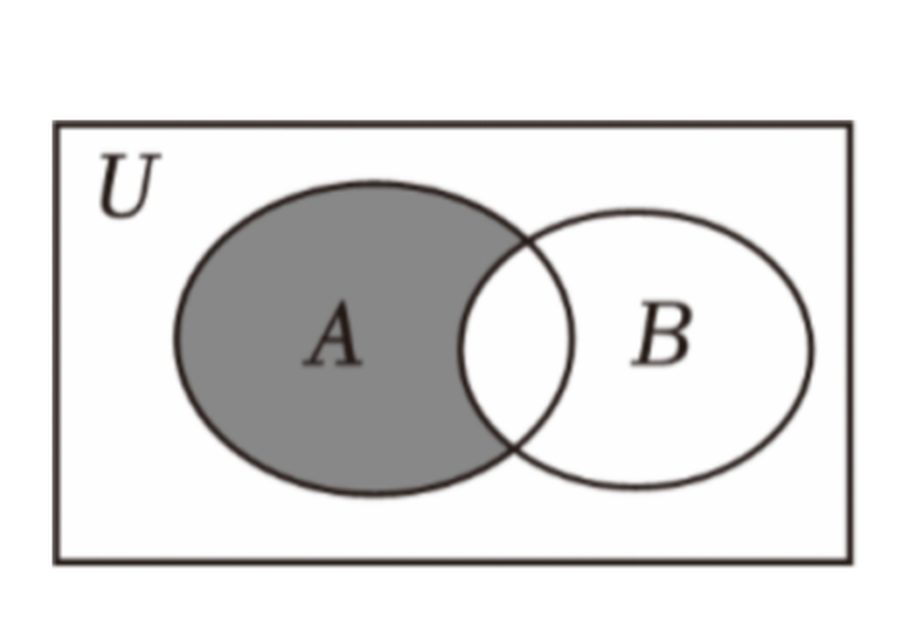
\includegraphics[width=0.34\textwidth]{figures/gao123_q17.png}
\end{center}

\ifanswer
\solbegin
\step{（1）$A\cap B=\{x\mid2\leqslant x\leqslant4\}$，}
\step{则图中阴影部分表示 $\overline{A\cap B}=\{x\mid-2\leqslant x<2\}$.}% 原卷把上划线盖在整个 $A\cap B$ 上，照录
\step{（2）由题意得 $\overline B=\{x\mid-6\leqslant x<2\}$，$C\subseteq B$，}
\step{所以当 $C=\varnothing$ 时，$10-a\geqslant2a+1$，解得 $a\leqslant3$，符合题意；}
\step{当 $C\neq\varnothing$ 时，$\begin{cases}10-a<2a+1\\2a+1\leqslant-6\end{cases}$ 或者 $\begin{cases}10-a<2a+1\\10-a\geqslant2\end{cases}$，}
\step{此时不等式组 $\begin{cases}10-a<2a+1\\2a+1\leqslant-6\end{cases}$ 无解，}
\step{不等式组 $\begin{cases}10-a<2a+1\\10-a\geqslant2\end{cases}$ 的解集为 $3<a\leqslant8$，}
\step{综上，$a$ 的取值范围为 $\{a\mid a\leqslant8\}$.}
\solend
\fi

\item (1) 求不等式：$\lvert x-1\rvert+\lvert x-2\rvert\leqslant5$ 的解集.

(2) 当 $m<1$ 时，解关于 $x$ 的不等式 $\dfrac{m(x-3)}{x+2}>1$.

\ifanswer
\solbegin
\step{(1) 当 $x<1$ 时，$\lvert x-1\rvert+\lvert x-2\rvert\leqslant5\Leftrightarrow-x+1+2-x\leqslant5$，}
\step{解得 $-1\leqslant x<1$；}
\step{当 $1\leqslant x\leqslant2$ 时，$\lvert x-1\rvert+\lvert x-2\rvert\leqslant5\Leftrightarrow x-1+2-x=1\leqslant5$ 恒成立，}
\step{所以 $1\leqslant x\leqslant2$；}
\step{当 $x>2$ 时，$\lvert x-1\rvert+\lvert x-2\rvert\leqslant5\Leftrightarrow x-1+x-2=2x-3\leqslant5$，}
\step{解得 $2<x\leqslant4$.}
\step{综上所述，不等式 $\lvert x-1\rvert+\lvert x-2\rvert\leqslant5$ 的解集为 $[-1,4]$.}
\step{(2) 原不等式变成 $\dfrac{(m-1)x-(3m+2)}{x+2}>0$，$n<1$，所以 $n-1<0$，}% 原卷作 $n<1$、$n-1<0$，与题设 $m<1$ 字母不一致，照录
\step{所以原不等式变成 $\dfrac{x-\dfrac{3m+2}{m-1}}{x+2}<0$，$\dfrac{3m+2}{m-1}-(-2)=\dfrac{5m}{m-1}$，}
\step{所以 $m<0$ 时，$\dfrac{5m}{m-1}>0$，$\dfrac{3m+2}{m-1}>-2$，}
\step{原不等式的解集为 $\left(-2,\dfrac{3m+2}{m-1}\right)$；}
\step{$m=0$ 时，原不等式变成 $1<0$，无解；}
\step{$0<m<1$ 时，$\dfrac{5m}{m-1}<0$，$\dfrac{3m+2}{m-1}<-2$，}
\step{原不等式的解集为 $\left(\dfrac{3m+2}{m-1},-2\right)$.}
\solend
\fi

\item 在园林博览会上，某公司带来了一种智能设备供采购商洽谈采购，并决定大量投放市场，已知该种设备年固定研发成本为 $50$ 万元，每生产一台需另投入 $100$ 元，设该公司一年内生产该设备 $x$ 万台且全部售完，每万台的销售收入 $G(x)$（万元）与年产量 $x$（万台）满足如下关系式：$G(x)=\begin{cases}180-x,0<x\leqslant20\\80+\dfrac{2000}{x}-\dfrac{8000}{x(x-1)},x>20\end{cases}$.

(1) 写出年利润 $W(x)$（万元）关于年产量 $x$（万台）的函数解析式；（利润 $=$ 销售收入 $-$ 成本）

(2) 当年产量为多少万台时，该公司获得的年利润最大，并求出最大利润.

\ifanswer
\solbegin
\step{(1) $W(x)=xG(x)-50-100x=\begin{cases}-50+80x-x^2,0<x\leqslant20\\-20x+1950-\dfrac{8000}{x-1},x>20\end{cases}$；}
\step{(2) 当 $0<x\leqslant20$ 时，$W(x)=-50+80x-x^2=-(x-40)^2+1550$，}
\step{由函数性质得当 $x\leqslant40$ 时严格增，所以当 $x=20$ 时，$W(x)_{max}=1150$，}
\step{当 $x>20$ 时，$W(x)=-20x+1950-\dfrac{8000}{x-1}=-20\left[(x-1)+\dfrac{400}{x-1}\right]+1930$，}
\step{$W(x)=-20\left[(x-1)+\dfrac{400}{x-1}\right]+1930\leqslant-20\times2\sqrt{(x-1)\cdot\dfrac{400}{x-1}}+1930$}
\step{$=1130$，当且仅当 $x-1=\dfrac{400}{x-1}$，即 $x=21$ 时取等号，}
\step{所以 $W(x)_{max}=1130$，}
\step{因为 $1150>1130$，所以当 $x=20$ 时，$W(x)_{max}=1150$，}
\step{即当年产量为 $20$ 万台时，该公司获得的年利润最大，}
\step{最大利润为 $1150$ 万元.}
\solend
\fi

\item 关于 $x$ 的方程 $(x^2-1)^2-2k\lvert x^2-1\rvert+k+1=0(k\in\R)$.

(1) 若方程无实根，求 $k$ 的取值范围；

(2) 若方程有 $4$ 个不等实根，求 $k$ 的取值范围；

(3) 若 $k=a+b$，且满足 $\dfrac1{a+2b}+\dfrac1{a+3}=\dfrac12$，$a>0$，$b>0$，试判断方程根的个数.

\ifanswer
\solbegin
\step{(1) 关于 $x$ 的方程 $(x^2-1)^2-2k\lvert x^2-1\rvert+k+1=0(k\in\R)$，}
\step{令 $t=\lvert x^2-1\rvert$，则 $t\geqslant0$，则原方程转化为 $t^2-2kt+k+1=0(*)$，}
\step{因为关于 $x$ 的方程 $(x^2-1)^2-2k\lvert x^2-1\rvert+k+1=0(k\in\R)$ 无实根，}
\step{所以 $(*)$ 式无实根或实根均小于零，令 $f(t)=t^2-2kt+k+1$，}
\step{①若 $(*)$ 式无实根，则 $\triangle<0$，解得 $\dfrac{1-\sqrt5}{2}<k<\dfrac{1+\sqrt5}{2}$，}
\step{②两根均为负，则 $\begin{cases}\Delta\geqslant0\\t_{\text{对}}=k<0\\f(0)>0\end{cases}$，解得 $-1<k\leqslant\dfrac{1-\sqrt5}{2}$，}
\step{综合①②，得 $k$ 的取值范围是 $\left(-1,\dfrac{1+\sqrt5}{2}\right)$；}
\step{(2) 作函数 $t=\lvert x^2-1\rvert$ 的图象，}
\begin{center}
% 图取原卷截图（第 11 页解析内）、去水印后 2× LANCZOS 放大，仅答案版出
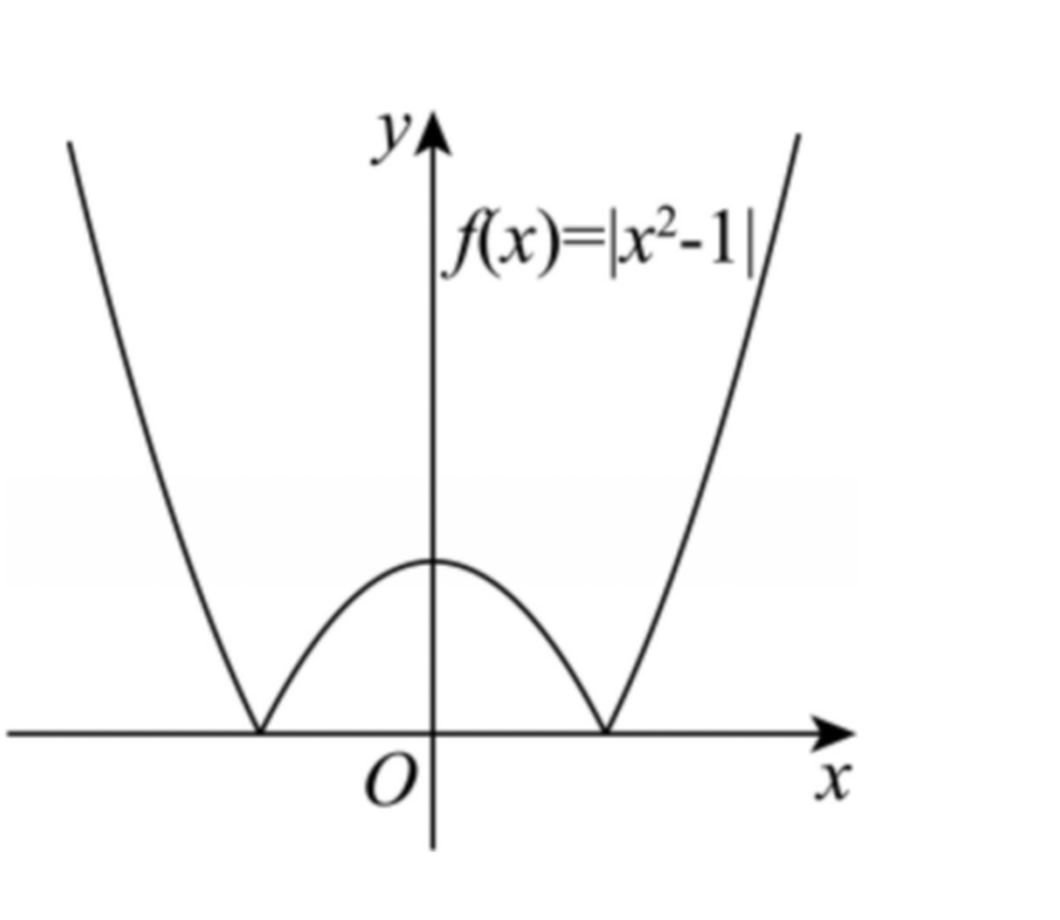
\includegraphics[width=0.40\textwidth]{figures/gao123_q20.png}
\end{center}
\step{$t=0$ 或 $t>1$ 时，每一个 $t$ 值对应 $2$ 个不同的 $x$ 值，}
\step{$t=1$ 时一个 $t$ 值对应 $3$ 个不同的 $x$ 值，}
\step{$0<t<1$ 时一个 $t$ 值对应 $4$ 个不同的 $x$ 值，}
\step{要使原方程有四个不等实根，}
\step{①$(*)$ 式一根为零，另一根大于 $1$，无解；}
\step{②$(*)$ 有两不等根且两根均大于 $1$，则 $\begin{cases}\Delta>0\\t_{\text{对}}=k>1\\f(1)>0\end{cases}$，解得 $\dfrac{1+\sqrt5}{2}<k<2$；}
\step{④$(*)$ 式有 $1$ 实根在 $(0,1)$ 之间，另一根小于零，}% 原卷由 ② 直接跳到 ④，缺 ③，照录
\step{则 $\begin{cases}f(0)<0\\f(1)>0\end{cases}$，所以 $\begin{cases}k+1<0\\2-k>0\end{cases}$，解得 $k<-1$，}
\step{综上所述，$k$ 取值范围为 $(-\infty,-1)\cup\left(\dfrac{1+\sqrt5}{2},2\right)$；}
\step{(3) 因为 $\dfrac1{a+2b}+\dfrac1{a+3}=\dfrac{a+2b+a+3}{(a+2b)(a+3)}=\dfrac{2(a+b)+3}{(a+2b)(a+3)}=\dfrac12$，}
\step{所以 $2(a+b)+3=\dfrac12(a+2b)(a+3)$，}
\step{因为 $a$、$b$ 为正实数，所以 $\dfrac12=\dfrac1{a+2b}+\dfrac1{a+3}\geqslant2\sqrt{\dfrac1{a+2b}\times\dfrac1{a+3}}$，}
\step{得 $\dfrac1{16}\geqslant\dfrac1{a+2b}\times\dfrac1{a+3}$，即 $(a+2b)(a+3)\geqslant16$，}
\step{所以 $2(a+b)+3\geqslant8$，即 $a+b\geqslant\dfrac52$，}
\step{当且仅当 $\dfrac1{a+2b}=\dfrac1{a+3}$ 即 $a=1$,$b=\dfrac32$ 时取等号，}
\step{故 $k\geqslant\dfrac52$，此时有 $\begin{cases}\Delta>0\\t_{\text{对}}=k>1\\f(0)>0,f(1)<0\end{cases}$，}
\step{故 $(*)$ 式有两不等实根且一根在 $(0,1)$ 之间，另一根大于 $1$，}
\step{故原方程有 $6$ 个实根.}
\solend
\fi

\item 设 $n$ 是不小于 $3$ 的正整数，集合 $S_n=\{(a_1,a_2,\cdots,a_n)\mid a_i\in\{0,1\},i=1,2,\cdots,n\}$，对于集合 $S_n$ 中任意两个元素 $A=(a_1,a_2,\cdots,a_n)$，$B=(b_1,b_2,\cdots,b_n)$.

定义 1：$A\cdot B=n-(\lvert a_1-b_1\rvert+\lvert a_2-b_2\rvert+\cdots+\lvert a_n-b_n\rvert)$，

定义 2：若 $A\cdot B=0$，则称互为相反元素，记作 $A=\overline B$ 或 $B=\overline A$.

(1) 若 $n=3$，$A=(0,1,0)$，$B=(1,1,0)$，试写出 $\overline A$、$\overline B$ 以及 $A\cdot B$ 的值；

(2) 若 $A$、$B\in S_n$，$A=(a_1,a_2,\cdots,a_n)$，$B=(b_1,b_2,\cdots,b_n)$，证明：$A\cdot B+\overline A\cdot B=n$；

(3) 设 $k$ 是小于 $n$ 的正奇数，至少含有两个元素的集合 $M\subseteq S_n$，且对于集合 $M$ 中任意两个不相同的元素 $A=(a_1,a_2,\cdots,a_n)$，$B=(b_1,b_2,\cdots,b_n)$，都有 $A\cdot B=n-k$，试求集合 $M$ 中元素个数的所有可能值.

\ifanswer
\solbegin
\step{(1) $\overline A=(1,0,1)$,$\overline B=(0,0,1)$,$\overline A\cdot\overline B=2$；}
\step{(2) 设 $A=(a_1,a_2,\cdots,a_n)$,$B=(b_1,b_2,\cdots,b_n)$,$\overline A=(x_1,x_2,\cdots,x_n)$，}
\step{由 $a_i$、$b_i$、$x_i\in\{0,1\}$，$i=1,2,\cdots,n$，得 $\lvert a_i-x_i\rvert\leqslant1$，$i=1,2,\cdots,n$，}
\step{所以 $\lvert a_1-x_1\rvert+\lvert a_2-x_2\rvert+\cdots+\lvert a_i-x_i\rvert\leqslant n$，}% 原卷末项下标作 $i$，照录
\step{当且仅当 $\lvert a_i-x_i\rvert=1$，$i=1,2,\cdots,n$，}
\step{即 $x_i=1-a_i$，$i=1,2,\cdots,n$ 时取等号.}
\step{由题意得 $A\cdot\overline A=n-(\lvert a_1-x_1\rvert+\lvert a_2-x_2\rvert+\cdots+\lvert a_n-x_n\rvert)=0$，}
\step{即 $\lvert a_1-x_1\rvert+\lvert a_2-x_2\rvert+\cdots+\lvert a_n-x_n\rvert=n$，}
\step{所以 $x_i=1-a_i$，$i=1,2,\cdots,n$，}
\step{$A\cdot B+\overline A\cdot B=2n-\sum\limits_{i=1}^n[\lvert a_i-b_i\rvert+(1-a_i)-b_i]$}
\step{$=2n-\sum\limits_{i=1}^n(\lvert1-b_i\rvert+\lvert0-b_i\rvert)=2n-\sum\limits_{i=1}^n(1-b_i+b_i)=2n-n=n$；}
\step{(3) 假设 $A=(a_1,a_2,\cdots,a_n)$，$B=(b_1,b_2,\cdots,b_n)$，$C=(c_1,c_2,\cdots,c_n)$}
\step{为集合 $M$ 中的三个不相同的元素，}
\step{则 $A\cdot B=n-(\lvert a_1-b_1\rvert+\lvert a_2-b_2\rvert+\cdots+\lvert a_n-b_n\rvert)=n-k$，}
\step{即 $\lvert a_1-b_1\rvert+\lvert a_2-b_2\rvert+\cdots+\lvert a_n-b_n\rvert=k$，}
\step{又由题意得 $\lvert a_i-b_i\rvert=0$ 或 $1$，$i=1,2,\cdots,n$，}
\step{$\lvert a_1-b_1\rvert$、$\lvert a_2-b_2\rvert$、$\cdots$、$\lvert a_n-b_n\rvert$ 恰有 $k$ 个 $1$，$n-k$ 个 $0$，}
\step{设其中 $k$ 个等于 $1$ 的项以此为 $a_{m_1}-b_{m_1}$,$a_{m_2}-b_{m_2}$,$\cdots$,$a_{m_k}-b_{m_k}$，}
\step{$n-k$ 个等于 $0$ 的项为 $a_{m_{k+1}}-b_{m_{k+1}}$,$a_{m_{k+2}}-b_{m_{k+2}}$,$\cdots$,$a_{m_n}-b_{m_n}$，}
\step{由题意得 $A\cdot C=n-(\lvert a_1-c_1\rvert+\lvert a_2-c_2\rvert+\cdots+\lvert a_n-c_n\rvert)=n-k$，}
\step{所以 $\sum\limits_{i=1}^k\lvert a_{m_i}-c_{m_i}\rvert+\sum\limits_{j=k+1}^n\lvert a_{m_j}-c_{m_j}\rvert=k$ ①，}
\step{同理 $\sum\limits_{i=1}^k\lvert b_{m_i}-c_{m_i}\rvert+\sum\limits_{j=k+1}^n\lvert b_{m_j}-c_{m_j}\rvert=k$ ②，}
\step{因为 $\lvert a_{m_{k+1}}-b_{m_{k+1}}\rvert=\lvert a_{m_{k+2}}-b_{m_{k+2}}\rvert=\cdots=\lvert a_{m_n}-b_{m_n}\rvert=0$，}
\step{所以 $\sum\limits_{j=k+1}^n\lvert a_{m_j}-c_{m_j}\rvert=\sum\limits_{j=k+1}^n\lvert b_{m_j}-c_{m_j}\rvert$，}
\step{由①$-$②得 $\sum\limits_{i=1}^k(\lvert a_{m_i}-c_{m_i}\rvert-\lvert b_{m_i}-c_{m_i}\rvert)=0$，}
\step{又 $\sum\limits_{i=1}^k(\lvert a_{m_i}-c_{m_i}\rvert-\lvert b_{m_i}-c_{m_i}\rvert)=\sum\limits_{i=1}^k(\lvert1-c_{m_i}\rvert-\lvert0-c_{m_i}\rvert)=k-2\sum\limits_{i=1}^k c_{m_i}$}
\step{为奇数，与 $\sum\limits_{i=1}^k(\lvert a_{m_i}-c_{m_i}\rvert-\lvert b_{m_i}-c_{m_i}\rvert)=0$ 矛盾，所以假设不成立，}
\step{即集合 $M$ 中至多有两个元素，}
\step{当 $M=\{(1,1,\cdots,1,0,0,\cdots,0),(0,0,\cdots,0)\}$ 时符合题意，}
\step{所以集合 $M$ 中元素的个数只可能是 $2$.}
\solend
\fi

\end{enumerate}

\end{document}
"
%
% 原始材料：微信公众号“魔都数学加油站”文章，作者破晓，2026-11-09 17:52 发布；
% 连载“27学年高一123”，原文标题“27学年高一123——2026-2027年上海市行知中学高一上10月月考”；
% 原文链接：https://mp.weixin.qq.com/s/GV4SWBLUJrBhMQwo22FVzg。
% 正文为 14 张 PNG 页（第 7、9、11、13、14 页 2560×3620，其余 4762×6735），
% 题目下印有【答案】或【解析】，为讲评版。
% 题目、解析均据原图转录；卷面红色水印及公众号页脚未录入。
% 全卷 3 张插图：第 5 题的坐标示意图、第 17 题的文氏图（均属题干，三版都出）、
% 第 20 题 (2) 的 $t=\lvert x^2-1\rvert$ 图象（属解析，仅答案版出）；
% 都取原卷截图去水印、2× LANCZOS 放大，见 figures/gao123_q5.png、
% figures/gao123_q17.png、figures/gao123_q20.png。
%
% 卷首标题：原卷印作“2026-2027 年行知中学高一上 10 月月考”（公众号标题中的“上海市”
% 卷面标题行没有，本稿照卷面），年份区间按全稿惯例排 en dash；原卷未印副标题，本稿按题目内容
% 标为“集合与常用逻辑用语、不等式”（与 110／111／113／116／118／120 同）。
%
% 与原卷的排版差异：
%   ① 原文从第 3 题起，填空题编号为 3—12、选择题为 13—16、解答题为 17—21，本稿保留原题号；
%   ② 原卷每题下直接印【解析】／【答案】，本稿按全稿惯例置于答案版；第 3 题只印【答案】、
%      另提 \ans{}；选择题答案在解析末句“故选 …”，括号内留空；
%   ③ 原卷未印副标题，本稿按“知识模块”口径补出；
%   ④ 原卷填空横线按全稿惯例排为 \blankline[4.4em]；选择题括号排 \mbox{（\quad）}、
%      选项段前按惯例加 \keepwithprev；解答题不留作答区（原卷为讲评版，与 109—122 同）；
%   ⑤ 原卷数集排斜体 $R$／$Z$（第 9 题作粗体 $\mathbf{R}$），按全稿惯例改 \R／\Z；
%      绝对值按全稿惯例排 \lvert…\rvert，集合描述竖线排 \mid；单位 km、h 原卷排斜体，
%      本稿按正体照排；补集照原卷上划线排 \overline{B}、\overline{A}。
%
% 判别式与子集符号：第 16 题解析的 $\triangle=b^2-4c<0$、第 20 题 (1) ① 的 $\triangle<0$
%   均作等边、扁的 \triangle；第 20 题 ② 两处 cases 与 (3) 的 $\Delta\geqslant0$／$\Delta>0$
%   作等腰、高的 \Delta，逐处照录、不统一；第 15 题选项与第 17 题 (2) 的 $\subseteq$
%   印有下划线，照录 \subseteq。
%
% 原卷存疑照录：
%   第 4 题解析“若 $-\lvert a\rvert=0$，则 $a=0$，则 $A=\{0,-1,0\}$”以元素重复说明互异性；
%   第 5 题解析“当 $a^2+b^2=400^2+b^2<500^2$”等式左边 $a^2$ 与 $400^2$ 并用；
%   第 9 题解析“解得 $a>1$ 得 $a<\dfrac13$”（按平方不等式应为 $a>1$ 或 $a<\dfrac13$）；
%   第 12 题解析“所以 $-\dfrac1{2^a}\cdot\dfrac1{2^b}\geqslant-\dfrac14$”带负号起论；
%   第 17 题 (1) 解析把阴影部分（实为 $A\cap\overline B$）印作 $\overline{A\cap B}$；
%   第 18 题 (2) 解析作“$n<1$，所以 $n-1<0$”，与题设 $m<1$ 字母不一致；
%   第 20 题 (2) 的情形编号由 ①、② 直接跳到 ④（缺 ③）；
%   第 21 题 (2) 解析“$\lvert a_1-x_1\rvert+\cdots+\lvert a_i-x_i\rvert\leqslant n$”
%   末项下标作 $i$（按上下文应为 $n$）。以上均照录加注。
%
% 行数核对：逐题数 \step 条数，合计 176 条（Q3：0；Q4：6；Q5：5；Q6：5；Q7：4；
% Q8：6；Q9：5；Q10：5；Q11：10；Q12：6；Q13：9；Q14：1；Q15：5；Q16：21；
% Q17：8；Q18：14；Q19：10；Q20：26；Q21：30），与原卷印刷行逐题相等
% （cases 块作一个印刷行计）。第 3 题只印【答案】，提 \ans{}，不计入 \step 账。
%
\documentclass[a4paper,11pt]{article}
\usepackage{common}

\begin{document}

\examtitlest[3]{2026--2027 年行知中学高一上 10 月月考}{集合与常用逻辑用语、不等式}

\bigsec{一、填空题}

\begin{enumerate}
\setcounter{enumi}{2}

\item 写出命题“存在实数 $x$、$y$、$z$，使 $x<y$ 或 $y<z$.”的否定\blankline[4.4em].

\ifanswer
\ans{任意实数 $x$、$y$、$z$，使得 $x\geqslant y$ 且 $y\geqslant z$}
\fi

\item 若集合 $\{0,-1,2a\}=\{a-1,-\lvert a\rvert,a+1\}$，实数 $a$ 的值为\blankline[4.4em].

\ifanswer
\solbegin
\step{令 $A=\{0,-1,2a\}$,$B=\{a-1,-\lvert a\rvert,a+1\}$，}
\step{因为 $\{0,-1,2a\}=\{a-1,-\lvert a\rvert,a+1\}$，}
\step{若 $a-1=0$，则 $a=1$，则 $A=\{0,-1,2\}$,$B=\{0,-1,2\}$，满足要求；}
\step{若 $-\lvert a\rvert=0$，则 $a=0$，则 $A=\{0,-1,0\}$，不满足集合元素的互异性；}% 原卷以 $A=\{0,-1,0\}$ 说明互异性，照录
\step{若 $a+1=0$，则 $a=-1$，则 $A=\{0,-1,-2\}$,$B=\{0,-1,-2\}$，满足要求；}
\step{故实数 $a$ 的值为 $\pm1$.}
\solend
\fi

\needvspace{7cm}
\item 如图，据气象部门预报，在距离某码头南偏东 $45^\circ$ 方向 $400\sqrt2$ km 处的热带
风暴中心正在以 $20$km/h 的速度向正北方向移动，距风暴中心 $500$km 以内
的地区都将受到影响. 以上预报估计，该码头将受到热带风暴的影响时长大
约为\blankline[4.4em]$h$.

\begin{center}
% 图取原卷截图（第 1 页题干右侧）、去水印后 2× LANCZOS 放大，本稿移至题干之后
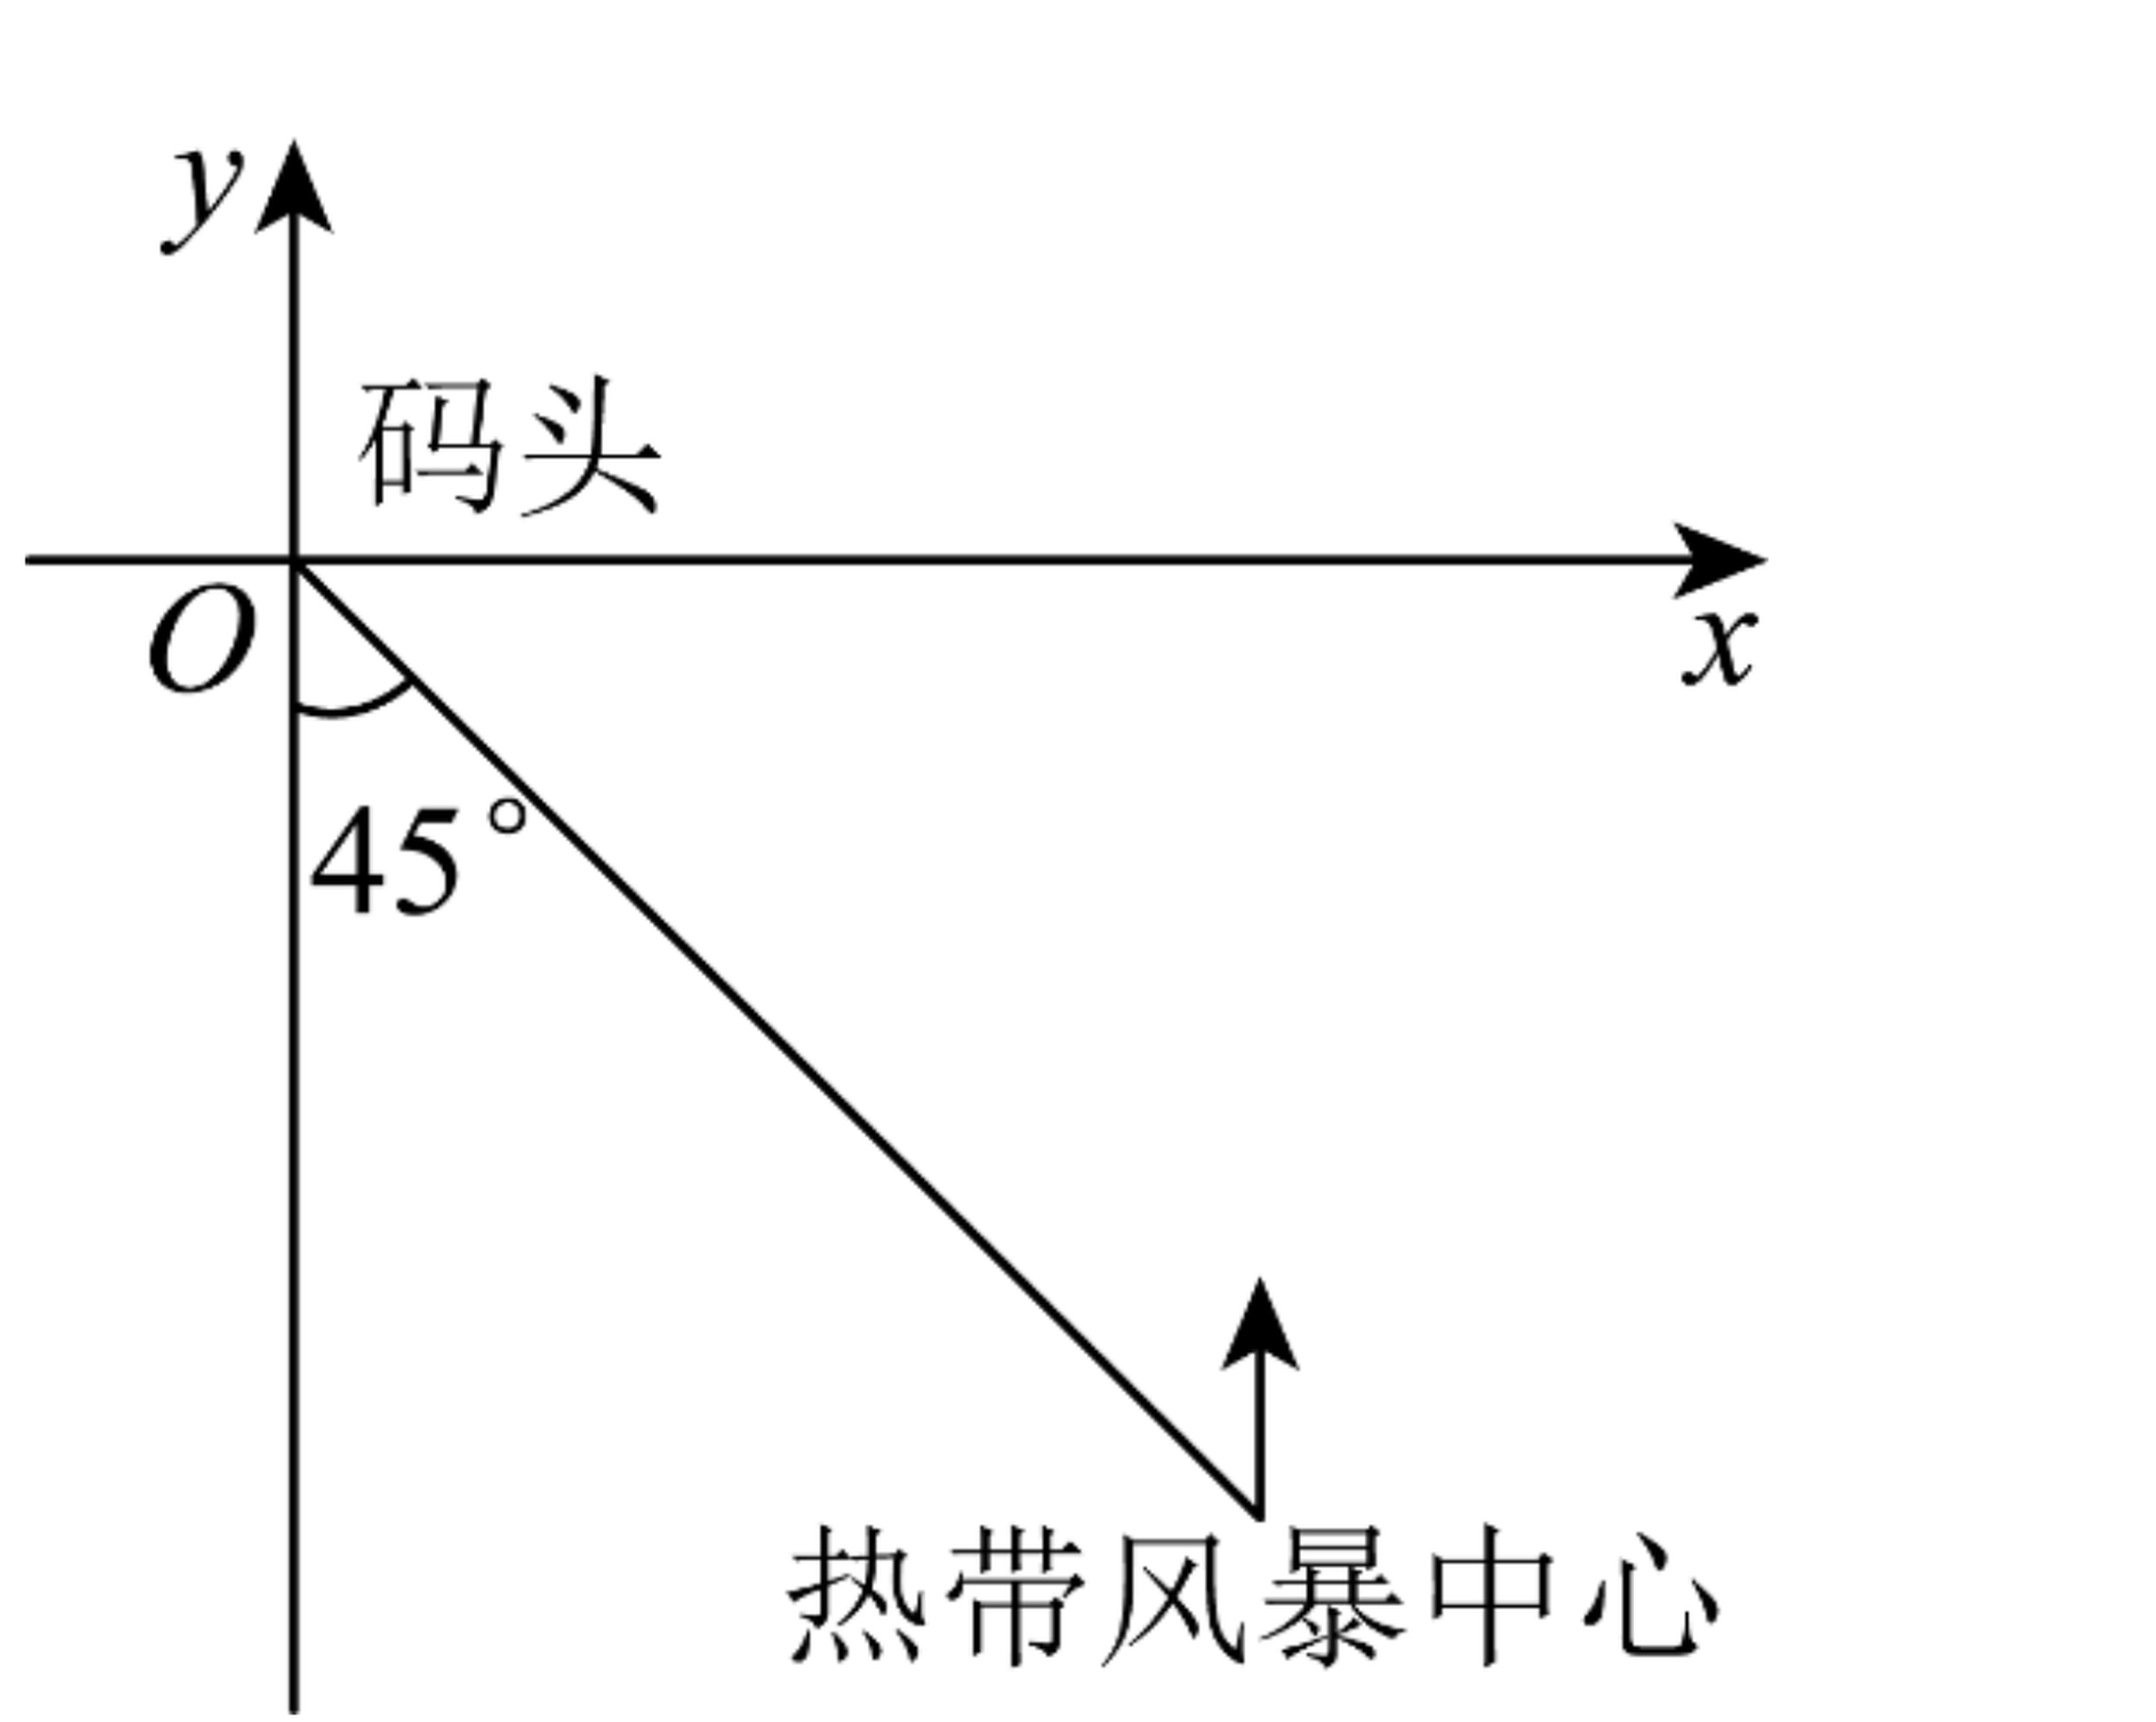
\includegraphics[width=0.36\textwidth]{figures/gao123_q5.png}
\end{center}

\ifanswer
\solbegin
\step{设风暴中心的坐标为 $(a,b)$，}
\step{由题意得 $a=400\sqrt2\times\cos45^\circ=400$，当 $a^2+b^2=400^2+b^2<500^2$，}% 原卷 $a^2$ 与 $400^2$ 并用，照录
\step{即 $-300<b<300$ 时，码头将受到风暴影响，}
\step{$\dfrac{300-(-300)}{20}=30h$，则码头受到风暴影响的时长为 30 小时，}
\step{所以由预报估计，该码头将受到热带风暴的影响时长大约为 30 小时.}
\solend
\fi

\item 已知 $a$、$b$、$c$ 为常数，若不等式 $\dfrac{ax-b}{x-c}\geqslant0$ 的解集为 $[-1,1)$，则不等式 $ax+b<0$ 的解集为\blankline[4.4em].

\ifanswer
\solbegin
\step{不等式 $\dfrac{ax-b}{x-c}\geqslant0$ 可化为 $(ax-b)(x-c)\geqslant0$ 且 $x-c\neq0$，}
\step{即 $a\left(x-\dfrac ba\right)(x-c)\geqslant0$ 且 $x\neq c$，}
\step{因为不等式 $\dfrac{ax-b}{x-c}\geqslant0$ 的解集为 $[-1,1)$，所以 $a<0$，且 $\dfrac ba=-1$,$c=1$，}
\step{即 $b=-a$，所以不等式 $ax+b<0$ 可化为 $ax-a<0$，又因为 $a<0$，所以 $x-1>0$，}
\step{解得 $x>1$，所以不等式 $ax+b<0$ 的解集为 $(1,+\infty)$.}
\solend
\fi

\item 已知实数 $a$、$b$ 满足 $ab=32$，且 $\log_2a=\log_b16$，则 $a+b$ 的值为\blankline[4.4em].

\ifanswer
\solbegin
\step{由 $\log_2a=\log_b16$，得 $\log_2a=\dfrac{\log_216}{\log_2b}$，则 $\log_2a\cdot\log_2b=4$，}
\step{由 $ab=32$，得 $\log_2a+\log_2b=\log_2ab=5$，}
\step{得 $\log_2a=1$,$\log_2b=4$ 或 $\log_2a=4$,$\log_2b=1$，}
\step{因此 $a=2$,$b=16$ 或 $a=16$,$b=2$，所以 $a+b=18$.}
\solend
\fi

\item 已知实数 $a$、$b$ 满足 $-3<a+2b<2$，$-1<2a-b<4$，则 $a+b$ 的取值范围为\blankline[4.4em].

\ifanswer
\solbegin
\step{设 $a+b=m(a+2b)+n(2a-b)=(m+2n)a+(2m-n)b$，}
\step{所以 $\begin{cases}m+2n=1\\2m-n=1\end{cases}$，解得 $n=\dfrac15$,$m=\dfrac35$，所以 $a+b=\dfrac35(a+2b)+\dfrac15(2a-b)$，}
\step{因为 $-3<(a+2b)<2$，$-1<2a-b<4$，}
\step{所以 $-\dfrac95<\dfrac35(a+2b)<\dfrac65$，$-\dfrac15<\dfrac15(2a-b)<\dfrac45$，}
\step{相加得 $-2<\dfrac35(a+2b)+\dfrac15(2a-b)<2$，即 $-2<a+b<2$，}
\step{故 $a+b$ 的取值范围为 $(-2,2)$.}
\solend
\fi

\item 存在 $x\in\R$ 使不等式 $\lvert2x-a\rvert<\lvert2a-1\rvert-2\lvert x\rvert$ 成立，则实数 $a$ 的取值范围是\blankline[4.4em].

\ifanswer
\solbegin
\step{存在 $x\in\R$，不等式 $\lvert2x-a\rvert<\lvert2a-1\rvert-2\lvert x\rvert$ 成立，}
\step{变形即 $\lvert2x-a\rvert+2\lvert x\rvert<\lvert2a-1\rvert$ 成立，}
\step{由于 $\lvert2x-a\rvert+\lvert2x\rvert\geqslant\lvert(2x-a)-2x\rvert=\lvert a\rvert$，当且仅当 $2x(2x-a)\leqslant0$ 时取等号，}
\step{因此有 $\lvert a\rvert<\lvert2a-1\rvert$，两边平方 $a^2<(2a-1)^2$，解得 $a>1$ 得 $a<\dfrac13$，}% 原卷“解得 a>1 得 a<1/3”，照录
\step{即实数 $a$ 的取值范围是 $\left(-\infty,\dfrac13\right)\cup(1,+\infty)$.}
\solend
\fi

\item 已知集合 $A=\{(x,y)\mid x^2+mx-y+2=0\}$，$B=\{(x,y)\mid x-y+1=0,0\leqslant x\leqslant3\}$，若集合 $A\cap B$ 的子集个数为 $2$，则实数 $m$ 的取值范围为\blankline[4.4em].

\ifanswer
\solbegin
\step{因为集合 $A\cap B$ 的子集个数为 $2$，所以 $A\cap B$ 的元素有一个，}
\step{即 $\begin{cases}x^2+mx-y+2=0\\x-y+1=0\end{cases}$ 在 $x\in[0,3]$ 上只有一个解，}
\step{即 $x^2+(m-1)x+1=0$ 在 $[0,3]$ 上只有一个解，}
\step{即 $1-m=x+\dfrac1x$ 在 $[0,3]$ 上只有一个解，}
\step{结合对勾函数的性质得 $1-m=2$ 或 $1-m>\dfrac{10}{3}$，解得 $m=-1$ 或 $m<-\dfrac73$.}
\solend
\fi

\item $[x]$ 表示不超过 $x$ 的最大整数，则集合 $A=\left\{y\,\middle\vert\,y=\left[\dfrac{x^2}{100}\right],x=1,2,3,\cdots,100\right\}$ 中的元素个数为\blankline[4.4em].

\ifanswer
\solbegin
\step{记 $a_k=\left[\dfrac{k^2}{100}\right](k=1,2,\cdots,100)$，$a_k$ 随 $k$ 增大而单调不减.}
\step{当 $k\geqslant50$ 时，$\dfrac{(k+1)^2}{100}-\dfrac{k^2}{100}=\dfrac{2k+1}{100}\geqslant\dfrac{101}{100}>1$，所以 $a_{k+1}\geqslant a_k+1$，}
\step{即 $a_{50}$、$a_{51}$、$\cdots$、$a_{100}$ 两两互异.}
\step{又 $a_{50}=\left[\dfrac{2500}{100}\right]=25$、$a_{100}=100$，这一段共 $100-50+1=51$ 个互异的值，}
\step{且都大于等于 $25$.}
\step{当 $k\leqslant49$ 时，$\dfrac{(k+1)^2}{100}-\dfrac{k^2}{100}=\dfrac{2k+1}{100}\leqslant\dfrac{99}{100}<1$，即 $a_k$ 每次至多增加 $1$；}
\step{又 $a_1=0$、$a_{49}=\left[\dfrac{2401}{100}\right]=24$，}
\step{故 $a_1$、$a_2$、$\cdots$、$a_{49}$ 依次取遍 $0$，$1$，$2$，$\cdots$，$24$，共 $25$ 个值.}
\step{两段取值范围互不重叠（前段不超过 $24$、后段不小于 $25$），}
\step{所以集合 $A$ 中共有 $25+51=76$ 个元素.}
\solend
\fi

\item 若实数 $a$、$b$、$c$ 满足 $\dfrac1{2^a}+\dfrac1{2^b}=1$，$\dfrac1{2^{a+b}}+\dfrac1{2^{b+c}}+\dfrac1{2^{a+c}}=1$，则 $c$ 的最大值是\blankline[4.4em].

\ifanswer
\solbegin
\step{因为 $\dfrac1{2^a}+\dfrac1{2^b}=1$，}
\step{由基本不等式得 $1=\dfrac1{2^a}+\dfrac1{2^b}\geqslant2\sqrt{\dfrac1{2^a}\cdot\dfrac1{2^b}}$（当且仅当 $a=b=1$ 时取等号），}
\step{所以 $\dfrac1{2^a}\cdot\dfrac1{2^b}\leqslant\dfrac14$，所以 $-\dfrac1{2^a}\cdot\dfrac1{2^b}\geqslant-\dfrac14$，}% 原卷带负号起论，照录
\step{因为 $\dfrac1{2^{a+b}}+\dfrac1{2^{b+c}}+\dfrac1{2^{a+c}}=1$，$\dfrac1{2^{b+c}}+\dfrac1{2^{a+c}}=\dfrac1{2^c}\left(\dfrac1{2^a}+\dfrac1{2^b}\right)=\dfrac1{2^c}$，}
\step{所以 $\dfrac1{2^c}=1-\dfrac1{2^{a+b}}\geqslant\dfrac34$，所以 $2^c\leqslant\dfrac43$，所以 $c\leqslant\log_2\dfrac43=2-\log_23$，}
\step{故 $c$ 的最大值是 $2-\log_23$.}
\solend
\fi

\end{enumerate}

\bigsec{二、选择题}

\begin{enumerate}
\setcounter{enumi}{12}

\item 下列运用等式或不等式的性质变形中，正确的是\mbox{（\quad）}

\keepwithprev
A. 如果 $a=b$，那么 $\dfrac ac=\dfrac bc$\qquad\qquad B. 如果 $\dfrac1a<\dfrac1b<0$，那么 $a-\dfrac1a>b-\dfrac1b$

C. 如果 $a>b$，那么 $\dfrac1a<\dfrac1b$\qquad\qquad D. 如果 $a>b>0$，$m\in\R$，那么 $\dfrac ba<\dfrac{b+m}{a+m}$

\ifanswer
\solbegin
\step{对于 $A$，若 $c=0$，$A$ 错误；}
\step{对于 $B$，若 $\dfrac1a<\dfrac1b<0$，则 $0>a>b$，$-\dfrac1a>-\dfrac1b>0$，}
\step{所以 $a-\dfrac1a>b-\dfrac1b$，$B$ 正确；}
\step{对于 $C$，$a>0$，$b<0$ 时，$C$ 错误；}
\step{对于 $D$，$\dfrac{b+m}{a+m}-\dfrac ba=\dfrac{ab+am}{a(a+m)}-\dfrac{ab+bm}{a(a+m)}=\dfrac{(a-b)m}{a(a+m)}$，}
\step{因为 $a>b>0$，所以 $a-b>0$，但 $m$、$a+m$ 的符号不确定，}
\step{当 $m=0$ 时，$\dfrac ba=\dfrac{b+m}{a+m}$，}
\step{当 $m(a+m)>0$ 时，$\dfrac ba<\dfrac{b+m}{a+m}$，当 $m(a+m)<0$ 时，$\dfrac ba>\dfrac{b+m}{a+m}$，$D$ 错误.}
\step{故选 $B$.}
\solend
\fi

\item “$a>b$”的一个必要非充分条件是\mbox{（\quad）}

\keepwithprev
A. $ac^2>bc^2$\qquad\quad B. $2^a>2^b$\qquad\quad C. $\left(\dfrac12\right)^{a-b}\leqslant1$\qquad\quad D. $a^3>b^3$

\ifanswer
\solbegin
\step{即“$a>b$”能推出选项，但选项不能推出“$a>b$”，故选 $C$.}
\solend
\fi

\item 若 $A=\left\{x\,\middle\vert\,x=\dfrac k6+1,k\in\Z\right\}$，$B=\left\{x\,\middle\vert\,x=\dfrac k3+\dfrac12,k\in\Z\right\}$，$C=\left\{x\,\middle\vert\,x=\dfrac{2k}{3}+\dfrac12,k\in\Z\right\}$，则这三个集合间的关系是\mbox{（\quad）}

\keepwithprev
A. $A\subseteq B\subseteq C$\qquad\quad B. $A\subseteq C\subseteq B$\qquad\quad C. $C\subseteq B\subseteq A$\qquad\quad D. $C\subseteq A\subseteq B$

\ifanswer
\solbegin
\step{若 $x\in C$，则存在 $k_0\in\Z$，使 $x=\dfrac{2k_0}{3}+\dfrac12$，}
\step{又 $2k_0\in\Z$，所以 $x\in B$，故 $C\subseteq B$，}
\step{若 $x\in B$，则存在 $k_1\in\Z$，使 $x=\dfrac{k_1}{3}+\dfrac12=\dfrac{2k_1-3}{6}+1$，}
\step{又 $2k_1-3\in\Z$，所以 $x\in A$，故 $B\subseteq A$，}
\step{又 $\dfrac43\in A$，$\dfrac43\notin B$，$\dfrac56\in B$，$\dfrac56\notin C$，所以 $C\subseteq B\subseteq A$，故选 $C$.}
\solend
\fi

\item 集合 $S=\{x\mid(x+a)(x^2+bx+c)=0\}$，$T=\{x\mid(ax+1)(cx^2+bx+1)=0\}$，其中 $a$、$b$、$c$ 为实数，若 $\lvert S\rvert$、$\lvert T\rvert$ 分别表示 $S$、$T$ 的元素个数，则下列结论中一定成立的是\mbox{（\quad）}

\keepwithprev
A. 若 $\lvert T\rvert=0$，则 $\lvert S\rvert=1$\qquad\qquad B. 若 $\lvert S\rvert=1$，则 $\lvert T\rvert=1$

C. 若 $\lvert S\rvert=2$，则 $\lvert T\rvert=2$\qquad\qquad D. 若 $\lvert T\rvert=3$，则 $\lvert S\rvert=2$

\ifanswer
\solbegin
\step{令 $f(x)=(x+a)(x^2+bx+c)$,$g(x)=(ax+1)(cx^2+bx+1)$，}
\step{对于选项 A，当 $\lvert T\rvert=0$ 时，方程 $g(x)=(ax+1)(cx^2+bx+1)=0$ 无实根，}
\step{当 $a=b=c=0$ 时，$f(x)=x^3$，由 $f(x)=0$ 得 $x=0$，此时 $\lvert S\rvert=1$；}
\step{当 $a=0$,$b^2-4c<0$ 时，$f(x)=x(x^2+bx+c)$，由 $f(x)=0$ 得 $x=0$，}
\step{此时 $\lvert S\rvert=1$，所以选项 A 正确；}
\step{对于选项 B，若 $\lvert S\rvert=1$，则 $f(x)=(x+a)(x^2+bx+c)=0$ 有且只有一根，}
\step{又 $x=-a$ 一定是 $f(x)=0$ 的根，所以 $\triangle=b^2-4c<0$，}
\step{又 $\triangle=b^2-4c<0$ 且 $a=0$ 时，$g(x)=(ax+1)(cx^2+bx+1)=0$ 无解，}
\step{此时 $\lvert T\rvert=0$，所以选项 B 错误，}
\step{对于选项 C，若 $\lvert S\rvert=2$ 时，则 $f(x)=(x+a)(x^2+bx+c)=0$ 有且只有 $2$ 根，}
\step{又 $x=-a$ 一定是 $f(x)=0$ 的根，}
\step{所以 $\triangle=b^2-4c=0$ 且 $a^2+ab+c\neq0$ 或 $\triangle=b^2-4c>0$ 且 $a^2+ab+c=0$，}
\step{当 $a=0$ 时，存在 $b$,$c$，使 $\triangle=b^2-4c=0$ 且 $a^2+ab+c\neq0$，}
\step{此时 $g(x)=(ax+1)(cx^2+bx+1)=0$ 只有一根，所以选项 C 错误，}
\step{对于选项 D，当 $\lvert T\rvert=3$ 时，方程 $g(x)=(ax+1)(cx^2+bx+1)=0$ 有三个根，}
\step{所以 $a\neq0$,$c\neq0$,$b^2-4c>0$，}
\step{设 $x_0$ 为 $g(x)=0$ 的一个根，即 $(ax_0+1)(cx_0^2+bx_0+1)=0$，}
\step{则 $x_0\neq0$，且 $f\left(\dfrac1{x_0}\right)=\left(\dfrac1{x_0}+a\right)\left(\dfrac1{x_0^2}+\dfrac1{x_0}b+c\right)=\dfrac1{x_0^3}g(x_0)=0$，}
\step{所以 $\dfrac1{x_0}$ 为方程 $f(x)=0$ 的根，故 $f(x)=0$ 有三个根，即 $\lvert T\rvert=3$ 时，}
\step{必有 $\lvert S\rvert=3$，所以选项 D 错误，}
\step{故选 $A$.}
\solend
\fi

\end{enumerate}

% 第 17 题是解答题第一题且带文氏图，守卫放在 \bigsec 之前，连节标题一起量页高
\needvspace{7cm}
\bigsec{三、解答题}

\begin{enumerate}
\setcounter{enumi}{16}

\item 设全集 $U=\R$，集合 $A=\{x\mid-2\leqslant x\leqslant4\}$，$B=\{x\mid x<-6$ 或 $x\geqslant2\}$.

（1）求图中阴影部分表示的集合；

（2）已知集合 $C=\{x\mid10-a<x<2a+1\}$，若 $\overline B\cap C=\varnothing$，求 $a$ 的取值范围.

\begin{center}
% 图取原卷截图（第 7 页题干右侧）、去水印后 2× LANCZOS 放大，本稿移至题干之后
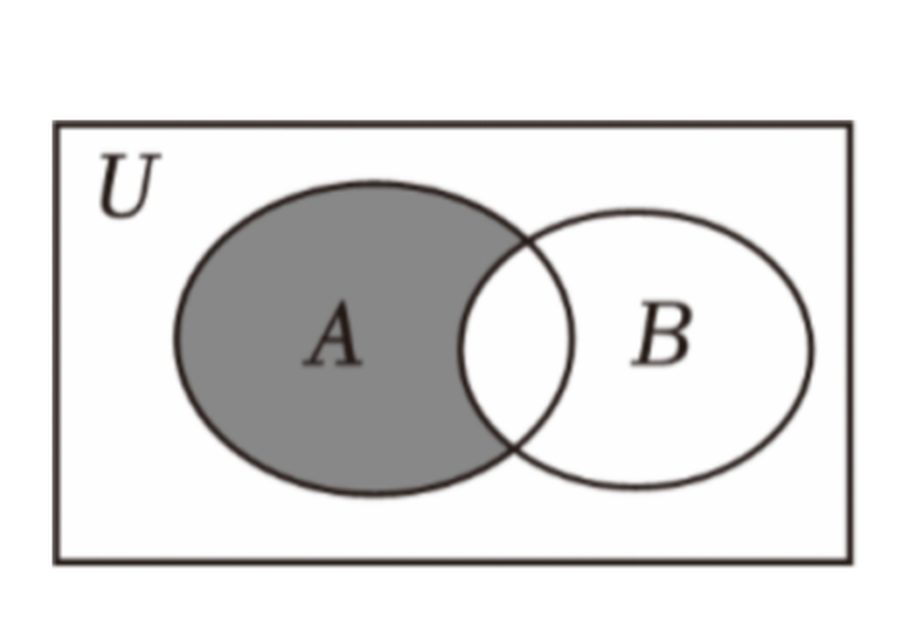
\includegraphics[width=0.34\textwidth]{figures/gao123_q17.png}
\end{center}

\ifanswer
\solbegin
\step{（1）$A\cap B=\{x\mid2\leqslant x\leqslant4\}$，}
\step{则图中阴影部分表示 $\overline{A\cap B}=\{x\mid-2\leqslant x<2\}$.}% 原卷把上划线盖在整个 $A\cap B$ 上，照录
\step{（2）由题意得 $\overline B=\{x\mid-6\leqslant x<2\}$，$C\subseteq B$，}
\step{所以当 $C=\varnothing$ 时，$10-a\geqslant2a+1$，解得 $a\leqslant3$，符合题意；}
\step{当 $C\neq\varnothing$ 时，$\begin{cases}10-a<2a+1\\2a+1\leqslant-6\end{cases}$ 或者 $\begin{cases}10-a<2a+1\\10-a\geqslant2\end{cases}$，}
\step{此时不等式组 $\begin{cases}10-a<2a+1\\2a+1\leqslant-6\end{cases}$ 无解，}
\step{不等式组 $\begin{cases}10-a<2a+1\\10-a\geqslant2\end{cases}$ 的解集为 $3<a\leqslant8$，}
\step{综上，$a$ 的取值范围为 $\{a\mid a\leqslant8\}$.}
\solend
\fi

\item (1) 求不等式：$\lvert x-1\rvert+\lvert x-2\rvert\leqslant5$ 的解集.

(2) 当 $m<1$ 时，解关于 $x$ 的不等式 $\dfrac{m(x-3)}{x+2}>1$.

\ifanswer
\solbegin
\step{(1) 当 $x<1$ 时，$\lvert x-1\rvert+\lvert x-2\rvert\leqslant5\Leftrightarrow-x+1+2-x\leqslant5$，}
\step{解得 $-1\leqslant x<1$；}
\step{当 $1\leqslant x\leqslant2$ 时，$\lvert x-1\rvert+\lvert x-2\rvert\leqslant5\Leftrightarrow x-1+2-x=1\leqslant5$ 恒成立，}
\step{所以 $1\leqslant x\leqslant2$；}
\step{当 $x>2$ 时，$\lvert x-1\rvert+\lvert x-2\rvert\leqslant5\Leftrightarrow x-1+x-2=2x-3\leqslant5$，}
\step{解得 $2<x\leqslant4$.}
\step{综上所述，不等式 $\lvert x-1\rvert+\lvert x-2\rvert\leqslant5$ 的解集为 $[-1,4]$.}
\step{(2) 原不等式变成 $\dfrac{(m-1)x-(3m+2)}{x+2}>0$，$n<1$，所以 $n-1<0$，}% 原卷作 $n<1$、$n-1<0$，与题设 $m<1$ 字母不一致，照录
\step{所以原不等式变成 $\dfrac{x-\dfrac{3m+2}{m-1}}{x+2}<0$，$\dfrac{3m+2}{m-1}-(-2)=\dfrac{5m}{m-1}$，}
\step{所以 $m<0$ 时，$\dfrac{5m}{m-1}>0$，$\dfrac{3m+2}{m-1}>-2$，}
\step{原不等式的解集为 $\left(-2,\dfrac{3m+2}{m-1}\right)$；}
\step{$m=0$ 时，原不等式变成 $1<0$，无解；}
\step{$0<m<1$ 时，$\dfrac{5m}{m-1}<0$，$\dfrac{3m+2}{m-1}<-2$，}
\step{原不等式的解集为 $\left(\dfrac{3m+2}{m-1},-2\right)$.}
\solend
\fi

\item 在园林博览会上，某公司带来了一种智能设备供采购商洽谈采购，并决定大量投放市场，已知该种设备年固定研发成本为 $50$ 万元，每生产一台需另投入 $100$ 元，设该公司一年内生产该设备 $x$ 万台且全部售完，每万台的销售收入 $G(x)$（万元）与年产量 $x$（万台）满足如下关系式：$G(x)=\begin{cases}180-x,0<x\leqslant20\\80+\dfrac{2000}{x}-\dfrac{8000}{x(x-1)},x>20\end{cases}$.

(1) 写出年利润 $W(x)$（万元）关于年产量 $x$（万台）的函数解析式；（利润 $=$ 销售收入 $-$ 成本）

(2) 当年产量为多少万台时，该公司获得的年利润最大，并求出最大利润.

\ifanswer
\solbegin
\step{(1) $W(x)=xG(x)-50-100x=\begin{cases}-50+80x-x^2,0<x\leqslant20\\-20x+1950-\dfrac{8000}{x-1},x>20\end{cases}$；}
\step{(2) 当 $0<x\leqslant20$ 时，$W(x)=-50+80x-x^2=-(x-40)^2+1550$，}
\step{由函数性质得当 $x\leqslant40$ 时严格增，所以当 $x=20$ 时，$W(x)_{max}=1150$，}
\step{当 $x>20$ 时，$W(x)=-20x+1950-\dfrac{8000}{x-1}=-20\left[(x-1)+\dfrac{400}{x-1}\right]+1930$，}
\step{$W(x)=-20\left[(x-1)+\dfrac{400}{x-1}\right]+1930\leqslant-20\times2\sqrt{(x-1)\cdot\dfrac{400}{x-1}}+1930$}
\step{$=1130$，当且仅当 $x-1=\dfrac{400}{x-1}$，即 $x=21$ 时取等号，}
\step{所以 $W(x)_{max}=1130$，}
\step{因为 $1150>1130$，所以当 $x=20$ 时，$W(x)_{max}=1150$，}
\step{即当年产量为 $20$ 万台时，该公司获得的年利润最大，}
\step{最大利润为 $1150$ 万元.}
\solend
\fi

\item 关于 $x$ 的方程 $(x^2-1)^2-2k\lvert x^2-1\rvert+k+1=0(k\in\R)$.

(1) 若方程无实根，求 $k$ 的取值范围；

(2) 若方程有 $4$ 个不等实根，求 $k$ 的取值范围；

(3) 若 $k=a+b$，且满足 $\dfrac1{a+2b}+\dfrac1{a+3}=\dfrac12$，$a>0$，$b>0$，试判断方程根的个数.

\ifanswer
\solbegin
\step{(1) 关于 $x$ 的方程 $(x^2-1)^2-2k\lvert x^2-1\rvert+k+1=0(k\in\R)$，}
\step{令 $t=\lvert x^2-1\rvert$，则 $t\geqslant0$，则原方程转化为 $t^2-2kt+k+1=0(*)$，}
\step{因为关于 $x$ 的方程 $(x^2-1)^2-2k\lvert x^2-1\rvert+k+1=0(k\in\R)$ 无实根，}
\step{所以 $(*)$ 式无实根或实根均小于零，令 $f(t)=t^2-2kt+k+1$，}
\step{①若 $(*)$ 式无实根，则 $\triangle<0$，解得 $\dfrac{1-\sqrt5}{2}<k<\dfrac{1+\sqrt5}{2}$，}
\step{②两根均为负，则 $\begin{cases}\Delta\geqslant0\\t_{\text{对}}=k<0\\f(0)>0\end{cases}$，解得 $-1<k\leqslant\dfrac{1-\sqrt5}{2}$，}
\step{综合①②，得 $k$ 的取值范围是 $\left(-1,\dfrac{1+\sqrt5}{2}\right)$；}
\step{(2) 作函数 $t=\lvert x^2-1\rvert$ 的图象，}
\begin{center}
% 图取原卷截图（第 11 页解析内）、去水印后 2× LANCZOS 放大，仅答案版出
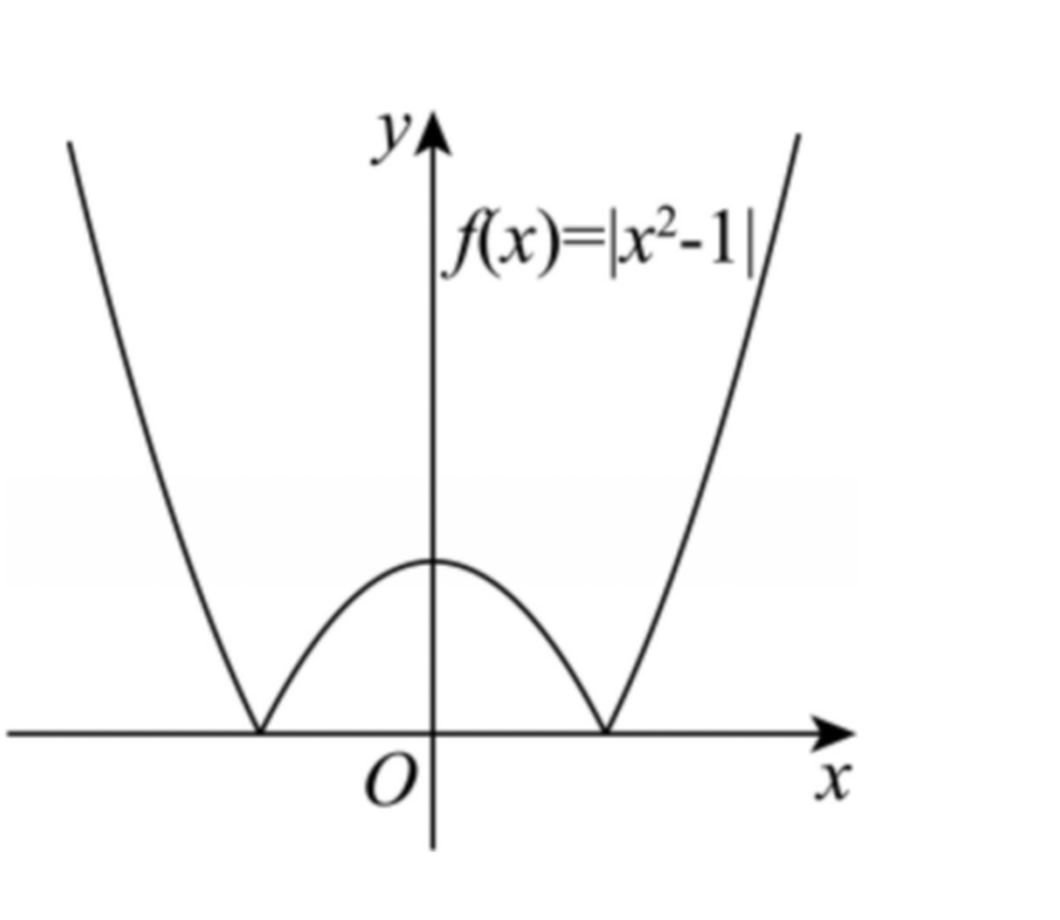
\includegraphics[width=0.40\textwidth]{figures/gao123_q20.png}
\end{center}
\step{$t=0$ 或 $t>1$ 时，每一个 $t$ 值对应 $2$ 个不同的 $x$ 值，}
\step{$t=1$ 时一个 $t$ 值对应 $3$ 个不同的 $x$ 值，}
\step{$0<t<1$ 时一个 $t$ 值对应 $4$ 个不同的 $x$ 值，}
\step{要使原方程有四个不等实根，}
\step{①$(*)$ 式一根为零，另一根大于 $1$，无解；}
\step{②$(*)$ 有两不等根且两根均大于 $1$，则 $\begin{cases}\Delta>0\\t_{\text{对}}=k>1\\f(1)>0\end{cases}$，解得 $\dfrac{1+\sqrt5}{2}<k<2$；}
\step{④$(*)$ 式有 $1$ 实根在 $(0,1)$ 之间，另一根小于零，}% 原卷由 ② 直接跳到 ④，缺 ③，照录
\step{则 $\begin{cases}f(0)<0\\f(1)>0\end{cases}$，所以 $\begin{cases}k+1<0\\2-k>0\end{cases}$，解得 $k<-1$，}
\step{综上所述，$k$ 取值范围为 $(-\infty,-1)\cup\left(\dfrac{1+\sqrt5}{2},2\right)$；}
\step{(3) 因为 $\dfrac1{a+2b}+\dfrac1{a+3}=\dfrac{a+2b+a+3}{(a+2b)(a+3)}=\dfrac{2(a+b)+3}{(a+2b)(a+3)}=\dfrac12$，}
\step{所以 $2(a+b)+3=\dfrac12(a+2b)(a+3)$，}
\step{因为 $a$、$b$ 为正实数，所以 $\dfrac12=\dfrac1{a+2b}+\dfrac1{a+3}\geqslant2\sqrt{\dfrac1{a+2b}\times\dfrac1{a+3}}$，}
\step{得 $\dfrac1{16}\geqslant\dfrac1{a+2b}\times\dfrac1{a+3}$，即 $(a+2b)(a+3)\geqslant16$，}
\step{所以 $2(a+b)+3\geqslant8$，即 $a+b\geqslant\dfrac52$，}
\step{当且仅当 $\dfrac1{a+2b}=\dfrac1{a+3}$ 即 $a=1$,$b=\dfrac32$ 时取等号，}
\step{故 $k\geqslant\dfrac52$，此时有 $\begin{cases}\Delta>0\\t_{\text{对}}=k>1\\f(0)>0,f(1)<0\end{cases}$，}
\step{故 $(*)$ 式有两不等实根且一根在 $(0,1)$ 之间，另一根大于 $1$，}
\step{故原方程有 $6$ 个实根.}
\solend
\fi

\item 设 $n$ 是不小于 $3$ 的正整数，集合 $S_n=\{(a_1,a_2,\cdots,a_n)\mid a_i\in\{0,1\},i=1,2,\cdots,n\}$，对于集合 $S_n$ 中任意两个元素 $A=(a_1,a_2,\cdots,a_n)$，$B=(b_1,b_2,\cdots,b_n)$.

定义 1：$A\cdot B=n-(\lvert a_1-b_1\rvert+\lvert a_2-b_2\rvert+\cdots+\lvert a_n-b_n\rvert)$，

定义 2：若 $A\cdot B=0$，则称互为相反元素，记作 $A=\overline B$ 或 $B=\overline A$.

(1) 若 $n=3$，$A=(0,1,0)$，$B=(1,1,0)$，试写出 $\overline A$、$\overline B$ 以及 $A\cdot B$ 的值；

(2) 若 $A$、$B\in S_n$，$A=(a_1,a_2,\cdots,a_n)$，$B=(b_1,b_2,\cdots,b_n)$，证明：$A\cdot B+\overline A\cdot B=n$；

(3) 设 $k$ 是小于 $n$ 的正奇数，至少含有两个元素的集合 $M\subseteq S_n$，且对于集合 $M$ 中任意两个不相同的元素 $A=(a_1,a_2,\cdots,a_n)$，$B=(b_1,b_2,\cdots,b_n)$，都有 $A\cdot B=n-k$，试求集合 $M$ 中元素个数的所有可能值.

\ifanswer
\solbegin
\step{(1) $\overline A=(1,0,1)$,$\overline B=(0,0,1)$,$\overline A\cdot\overline B=2$；}
\step{(2) 设 $A=(a_1,a_2,\cdots,a_n)$,$B=(b_1,b_2,\cdots,b_n)$,$\overline A=(x_1,x_2,\cdots,x_n)$，}
\step{由 $a_i$、$b_i$、$x_i\in\{0,1\}$，$i=1,2,\cdots,n$，得 $\lvert a_i-x_i\rvert\leqslant1$，$i=1,2,\cdots,n$，}
\step{所以 $\lvert a_1-x_1\rvert+\lvert a_2-x_2\rvert+\cdots+\lvert a_i-x_i\rvert\leqslant n$，}% 原卷末项下标作 $i$，照录
\step{当且仅当 $\lvert a_i-x_i\rvert=1$，$i=1,2,\cdots,n$，}
\step{即 $x_i=1-a_i$，$i=1,2,\cdots,n$ 时取等号.}
\step{由题意得 $A\cdot\overline A=n-(\lvert a_1-x_1\rvert+\lvert a_2-x_2\rvert+\cdots+\lvert a_n-x_n\rvert)=0$，}
\step{即 $\lvert a_1-x_1\rvert+\lvert a_2-x_2\rvert+\cdots+\lvert a_n-x_n\rvert=n$，}
\step{所以 $x_i=1-a_i$，$i=1,2,\cdots,n$，}
\step{$A\cdot B+\overline A\cdot B=2n-\sum\limits_{i=1}^n[\lvert a_i-b_i\rvert+(1-a_i)-b_i]$}
\step{$=2n-\sum\limits_{i=1}^n(\lvert1-b_i\rvert+\lvert0-b_i\rvert)=2n-\sum\limits_{i=1}^n(1-b_i+b_i)=2n-n=n$；}
\step{(3) 假设 $A=(a_1,a_2,\cdots,a_n)$，$B=(b_1,b_2,\cdots,b_n)$，$C=(c_1,c_2,\cdots,c_n)$}
\step{为集合 $M$ 中的三个不相同的元素，}
\step{则 $A\cdot B=n-(\lvert a_1-b_1\rvert+\lvert a_2-b_2\rvert+\cdots+\lvert a_n-b_n\rvert)=n-k$，}
\step{即 $\lvert a_1-b_1\rvert+\lvert a_2-b_2\rvert+\cdots+\lvert a_n-b_n\rvert=k$，}
\step{又由题意得 $\lvert a_i-b_i\rvert=0$ 或 $1$，$i=1,2,\cdots,n$，}
\step{$\lvert a_1-b_1\rvert$、$\lvert a_2-b_2\rvert$、$\cdots$、$\lvert a_n-b_n\rvert$ 恰有 $k$ 个 $1$，$n-k$ 个 $0$，}
\step{设其中 $k$ 个等于 $1$ 的项以此为 $a_{m_1}-b_{m_1}$,$a_{m_2}-b_{m_2}$,$\cdots$,$a_{m_k}-b_{m_k}$，}
\step{$n-k$ 个等于 $0$ 的项为 $a_{m_{k+1}}-b_{m_{k+1}}$,$a_{m_{k+2}}-b_{m_{k+2}}$,$\cdots$,$a_{m_n}-b_{m_n}$，}
\step{由题意得 $A\cdot C=n-(\lvert a_1-c_1\rvert+\lvert a_2-c_2\rvert+\cdots+\lvert a_n-c_n\rvert)=n-k$，}
\step{所以 $\sum\limits_{i=1}^k\lvert a_{m_i}-c_{m_i}\rvert+\sum\limits_{j=k+1}^n\lvert a_{m_j}-c_{m_j}\rvert=k$ ①，}
\step{同理 $\sum\limits_{i=1}^k\lvert b_{m_i}-c_{m_i}\rvert+\sum\limits_{j=k+1}^n\lvert b_{m_j}-c_{m_j}\rvert=k$ ②，}
\step{因为 $\lvert a_{m_{k+1}}-b_{m_{k+1}}\rvert=\lvert a_{m_{k+2}}-b_{m_{k+2}}\rvert=\cdots=\lvert a_{m_n}-b_{m_n}\rvert=0$，}
\step{所以 $\sum\limits_{j=k+1}^n\lvert a_{m_j}-c_{m_j}\rvert=\sum\limits_{j=k+1}^n\lvert b_{m_j}-c_{m_j}\rvert$，}
\step{由①$-$②得 $\sum\limits_{i=1}^k(\lvert a_{m_i}-c_{m_i}\rvert-\lvert b_{m_i}-c_{m_i}\rvert)=0$，}
\step{又 $\sum\limits_{i=1}^k(\lvert a_{m_i}-c_{m_i}\rvert-\lvert b_{m_i}-c_{m_i}\rvert)=\sum\limits_{i=1}^k(\lvert1-c_{m_i}\rvert-\lvert0-c_{m_i}\rvert)=k-2\sum\limits_{i=1}^k c_{m_i}$}
\step{为奇数，与 $\sum\limits_{i=1}^k(\lvert a_{m_i}-c_{m_i}\rvert-\lvert b_{m_i}-c_{m_i}\rvert)=0$ 矛盾，所以假设不成立，}
\step{即集合 $M$ 中至多有两个元素，}
\step{当 $M=\{(1,1,\cdots,1,0,0,\cdots,0),(0,0,\cdots,0)\}$ 时符合题意，}
\step{所以集合 $M$ 中元素的个数只可能是 $2$.}
\solend
\fi

\end{enumerate}

\end{document}
"
%
% 原始材料：微信公众号“魔都数学加油站”文章，作者破晓，2026-11-09 17:52 发布；
% 连载“27学年高一123”，原文标题“27学年高一123——2026-2027年上海市行知中学高一上10月月考”；
% 原文链接：https://mp.weixin.qq.com/s/GV4SWBLUJrBhMQwo22FVzg。
% 正文为 14 张 PNG 页（第 7、9、11、13、14 页 2560×3620，其余 4762×6735），
% 题目下印有【答案】或【解析】，为讲评版。
% 题目、解析均据原图转录；卷面红色水印及公众号页脚未录入。
% 全卷 3 张插图：第 5 题的坐标示意图、第 17 题的文氏图（均属题干，三版都出）、
% 第 20 题 (2) 的 $t=\lvert x^2-1\rvert$ 图象（属解析，仅答案版出）；
% 都取原卷截图去水印、2× LANCZOS 放大，见 figures/gao123_q5.png、
% figures/gao123_q17.png、figures/gao123_q20.png。
%
% 卷首标题：原卷印作“2026-2027 年行知中学高一上 10 月月考”（公众号标题中的“上海市”
% 卷面标题行没有，本稿照卷面），年份区间按全稿惯例排 en dash；原卷未印副标题，本稿按题目内容
% 标为“集合与常用逻辑用语、不等式”（与 110／111／113／116／118／120 同）。
%
% 与原卷的排版差异：
%   ① 原文从第 3 题起，填空题编号为 3—12、选择题为 13—16、解答题为 17—21，本稿保留原题号；
%   ② 原卷每题下直接印【解析】／【答案】，本稿按全稿惯例置于答案版；第 3 题只印【答案】、
%      另提 \ans{}；选择题答案在解析末句“故选 …”，括号内留空；
%   ③ 原卷未印副标题，本稿按“知识模块”口径补出；
%   ④ 原卷填空横线按全稿惯例排为 \blankline[4.4em]；选择题括号排 \mbox{（\quad）}、
%      选项段前按惯例加 \keepwithprev；解答题不留作答区（原卷为讲评版，与 109—122 同）；
%   ⑤ 原卷数集排斜体 $R$／$Z$（第 9 题作粗体 $\mathbf{R}$），按全稿惯例改 \R／\Z；
%      绝对值按全稿惯例排 \lvert…\rvert，集合描述竖线排 \mid；单位 km、h 原卷排斜体，
%      本稿按正体照排；补集照原卷上划线排 \overline{B}、\overline{A}。
%
% 判别式与子集符号：第 16 题解析的 $\triangle=b^2-4c<0$、第 20 题 (1) ① 的 $\triangle<0$
%   均作等边、扁的 \triangle；第 20 题 ② 两处 cases 与 (3) 的 $\Delta\geqslant0$／$\Delta>0$
%   作等腰、高的 \Delta，逐处照录、不统一；第 15 题选项与第 17 题 (2) 的 $\subseteq$
%   印有下划线，照录 \subseteq。
%
% 原卷存疑照录：
%   第 4 题解析“若 $-\lvert a\rvert=0$，则 $a=0$，则 $A=\{0,-1,0\}$”以元素重复说明互异性；
%   第 5 题解析“当 $a^2+b^2=400^2+b^2<500^2$”等式左边 $a^2$ 与 $400^2$ 并用；
%   第 9 题解析“解得 $a>1$ 得 $a<\dfrac13$”（按平方不等式应为 $a>1$ 或 $a<\dfrac13$）；
%   第 12 题解析“所以 $-\dfrac1{2^a}\cdot\dfrac1{2^b}\geqslant-\dfrac14$”带负号起论；
%   第 17 题 (1) 解析把阴影部分（实为 $A\cap\overline B$）印作 $\overline{A\cap B}$；
%   第 18 题 (2) 解析作“$n<1$，所以 $n-1<0$”，与题设 $m<1$ 字母不一致；
%   第 20 题 (2) 的情形编号由 ①、② 直接跳到 ④（缺 ③）；
%   第 21 题 (2) 解析“$\lvert a_1-x_1\rvert+\cdots+\lvert a_i-x_i\rvert\leqslant n$”
%   末项下标作 $i$（按上下文应为 $n$）。以上均照录加注。
%
% 行数核对：逐题数 \step 条数，合计 176 条（Q3：0；Q4：6；Q5：5；Q6：5；Q7：4；
% Q8：6；Q9：5；Q10：5；Q11：10；Q12：6；Q13：9；Q14：1；Q15：5；Q16：21；
% Q17：8；Q18：14；Q19：10；Q20：26；Q21：30），与原卷印刷行逐题相等
% （cases 块作一个印刷行计）。第 3 题只印【答案】，提 \ans{}，不计入 \step 账。
%
\documentclass[a4paper,11pt]{article}
\usepackage{common}

\begin{document}

\examtitlest[3]{2026--2027 年行知中学高一上 10 月月考}{集合与常用逻辑用语、不等式}

\bigsec{一、填空题}

\begin{enumerate}
\setcounter{enumi}{2}

\item 写出命题“存在实数 $x$、$y$、$z$，使 $x<y$ 或 $y<z$.”的否定\blankline[4.4em].

\ifanswer
\ans{任意实数 $x$、$y$、$z$，使得 $x\geqslant y$ 且 $y\geqslant z$}
\fi

\item 若集合 $\{0,-1,2a\}=\{a-1,-\lvert a\rvert,a+1\}$，实数 $a$ 的值为\blankline[4.4em].

\ifanswer
\solbegin
\step{令 $A=\{0,-1,2a\}$,$B=\{a-1,-\lvert a\rvert,a+1\}$，}
\step{因为 $\{0,-1,2a\}=\{a-1,-\lvert a\rvert,a+1\}$，}
\step{若 $a-1=0$，则 $a=1$，则 $A=\{0,-1,2\}$,$B=\{0,-1,2\}$，满足要求；}
\step{若 $-\lvert a\rvert=0$，则 $a=0$，则 $A=\{0,-1,0\}$，不满足集合元素的互异性；}% 原卷以 $A=\{0,-1,0\}$ 说明互异性，照录
\step{若 $a+1=0$，则 $a=-1$，则 $A=\{0,-1,-2\}$,$B=\{0,-1,-2\}$，满足要求；}
\step{故实数 $a$ 的值为 $\pm1$.}
\solend
\fi

\needvspace{7cm}
\item 如图，据气象部门预报，在距离某码头南偏东 $45^\circ$ 方向 $400\sqrt2$ km 处的热带
风暴中心正在以 $20$km/h 的速度向正北方向移动，距风暴中心 $500$km 以内
的地区都将受到影响. 以上预报估计，该码头将受到热带风暴的影响时长大
约为\blankline[4.4em]$h$.

\begin{center}
% 图取原卷截图（第 1 页题干右侧）、去水印后 2× LANCZOS 放大，本稿移至题干之后
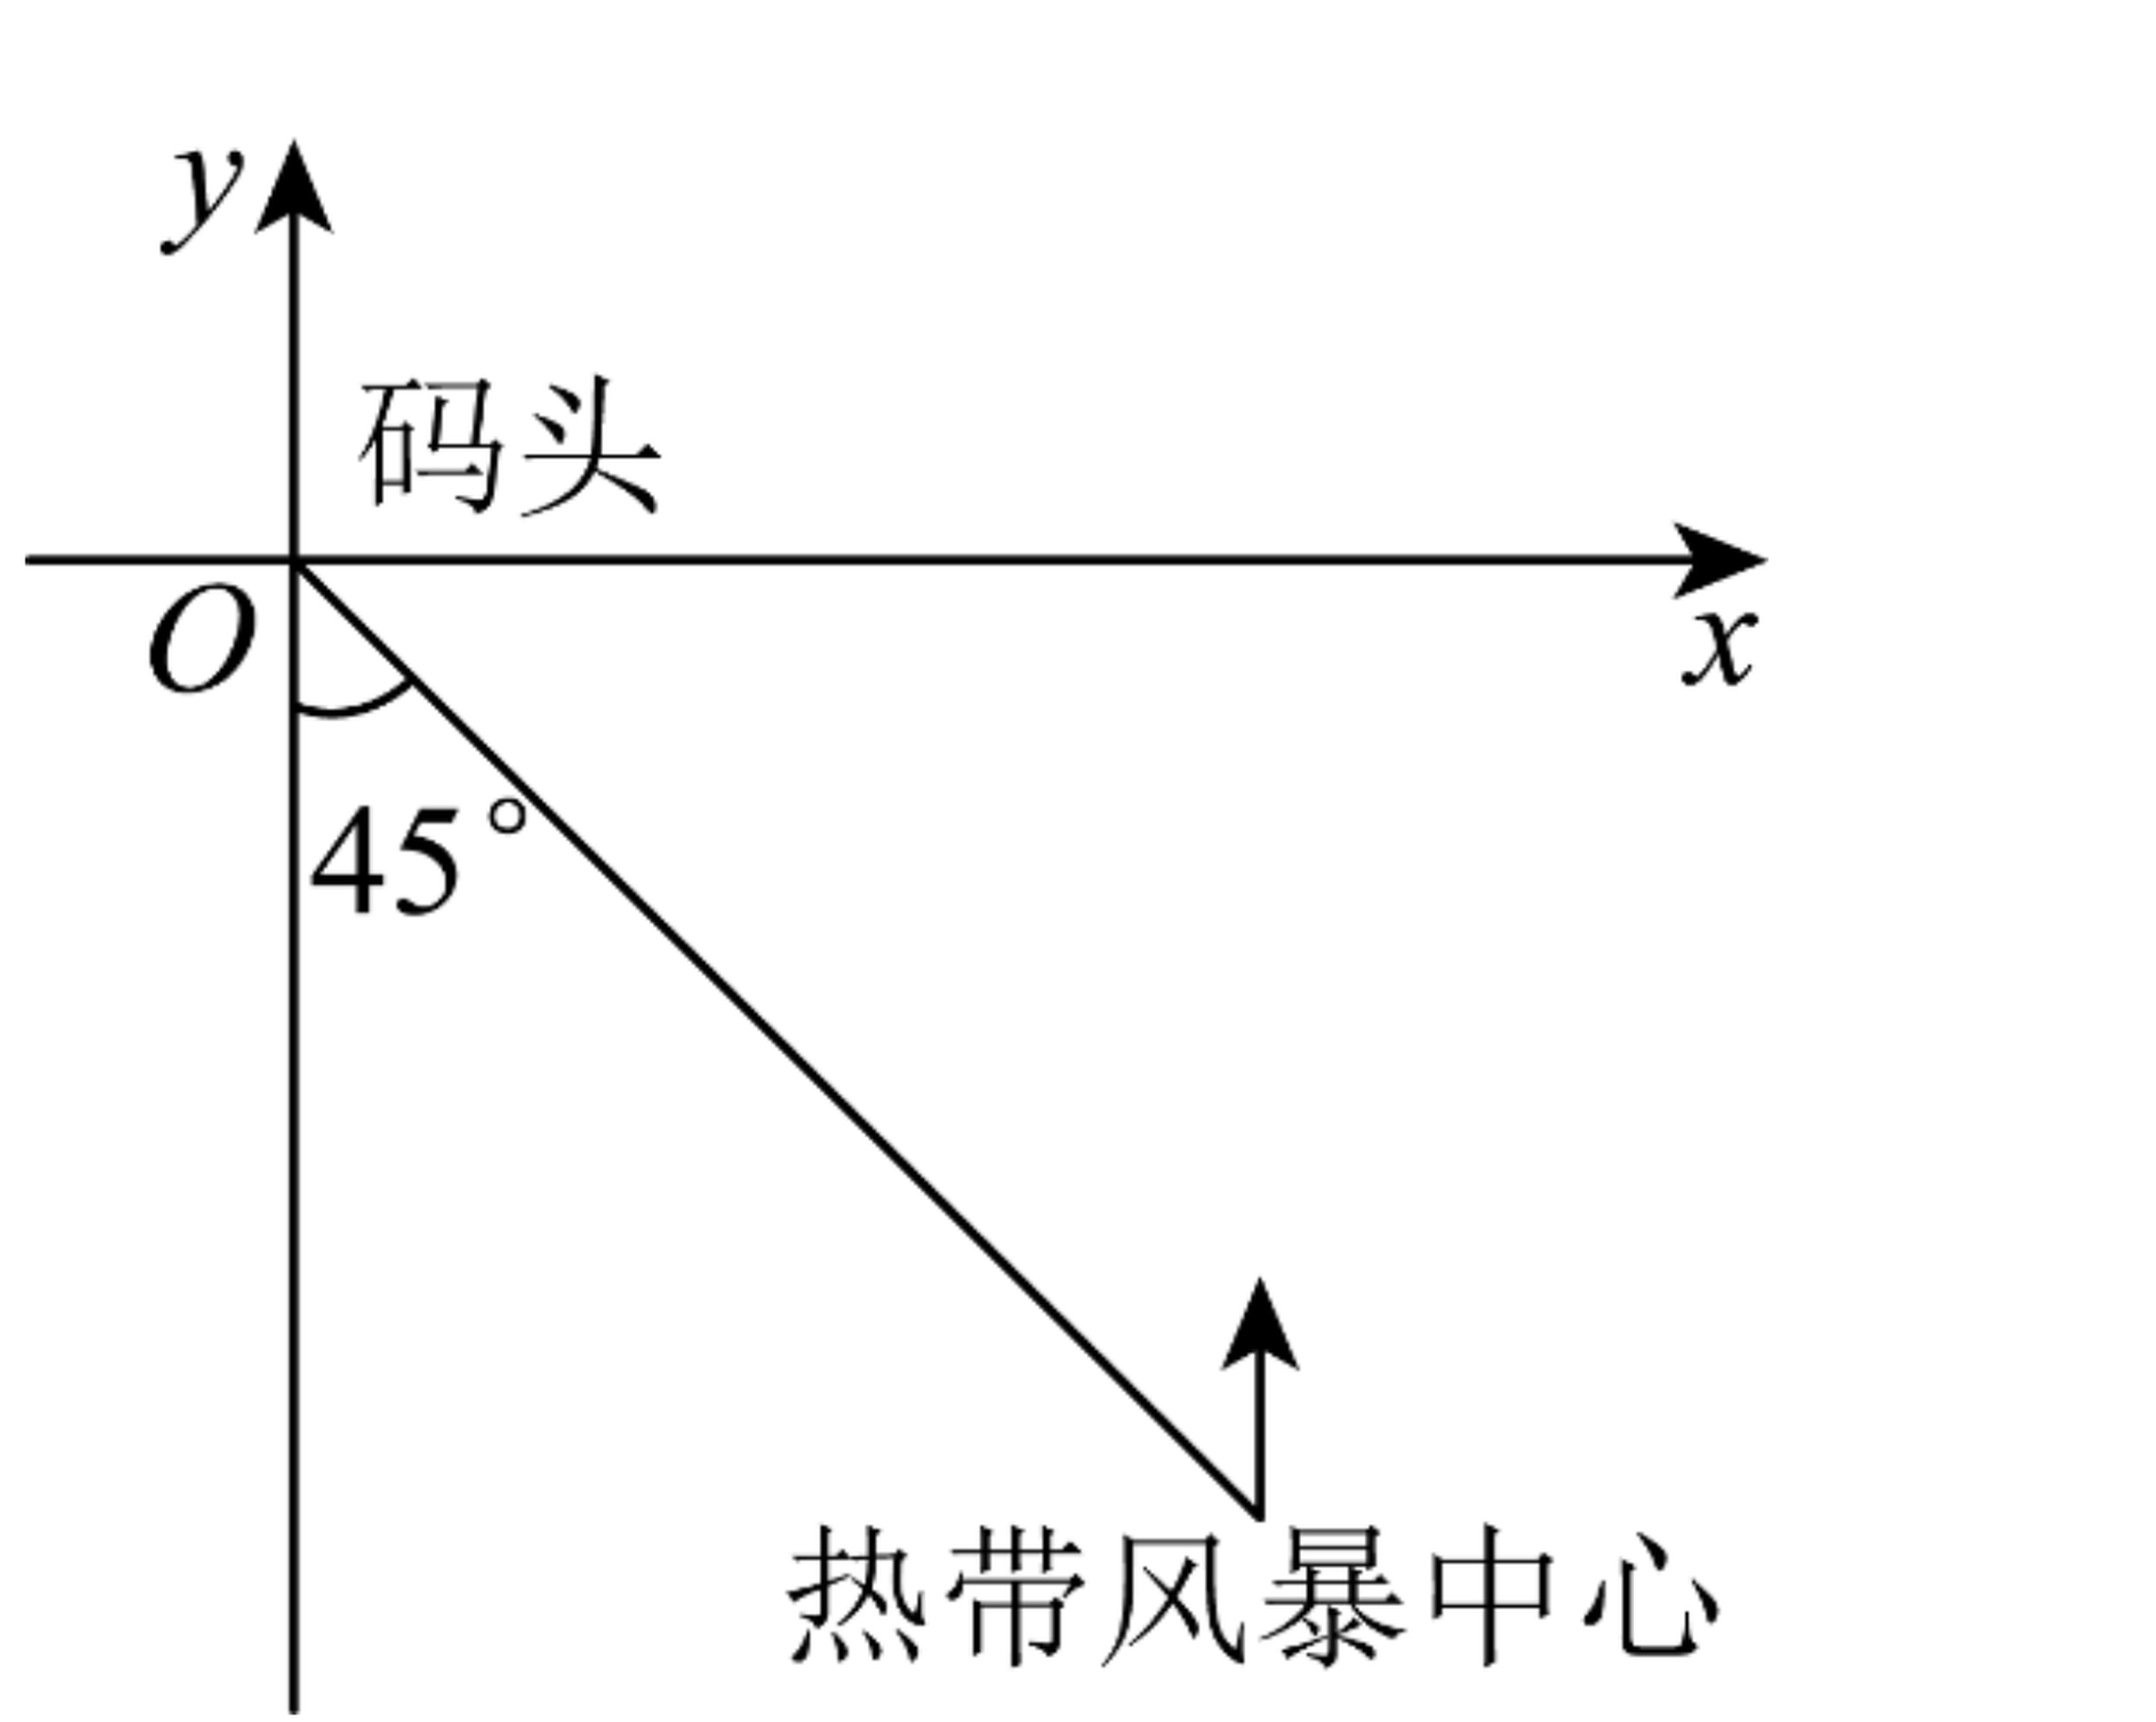
\includegraphics[width=0.36\textwidth]{figures/gao123_q5.png}
\end{center}

\ifanswer
\solbegin
\step{设风暴中心的坐标为 $(a,b)$，}
\step{由题意得 $a=400\sqrt2\times\cos45^\circ=400$，当 $a^2+b^2=400^2+b^2<500^2$，}% 原卷 $a^2$ 与 $400^2$ 并用，照录
\step{即 $-300<b<300$ 时，码头将受到风暴影响，}
\step{$\dfrac{300-(-300)}{20}=30h$，则码头受到风暴影响的时长为 30 小时，}
\step{所以由预报估计，该码头将受到热带风暴的影响时长大约为 30 小时.}
\solend
\fi

\item 已知 $a$、$b$、$c$ 为常数，若不等式 $\dfrac{ax-b}{x-c}\geqslant0$ 的解集为 $[-1,1)$，则不等式 $ax+b<0$ 的解集为\blankline[4.4em].

\ifanswer
\solbegin
\step{不等式 $\dfrac{ax-b}{x-c}\geqslant0$ 可化为 $(ax-b)(x-c)\geqslant0$ 且 $x-c\neq0$，}
\step{即 $a\left(x-\dfrac ba\right)(x-c)\geqslant0$ 且 $x\neq c$，}
\step{因为不等式 $\dfrac{ax-b}{x-c}\geqslant0$ 的解集为 $[-1,1)$，所以 $a<0$，且 $\dfrac ba=-1$,$c=1$，}
\step{即 $b=-a$，所以不等式 $ax+b<0$ 可化为 $ax-a<0$，又因为 $a<0$，所以 $x-1>0$，}
\step{解得 $x>1$，所以不等式 $ax+b<0$ 的解集为 $(1,+\infty)$.}
\solend
\fi

\item 已知实数 $a$、$b$ 满足 $ab=32$，且 $\log_2a=\log_b16$，则 $a+b$ 的值为\blankline[4.4em].

\ifanswer
\solbegin
\step{由 $\log_2a=\log_b16$，得 $\log_2a=\dfrac{\log_216}{\log_2b}$，则 $\log_2a\cdot\log_2b=4$，}
\step{由 $ab=32$，得 $\log_2a+\log_2b=\log_2ab=5$，}
\step{得 $\log_2a=1$,$\log_2b=4$ 或 $\log_2a=4$,$\log_2b=1$，}
\step{因此 $a=2$,$b=16$ 或 $a=16$,$b=2$，所以 $a+b=18$.}
\solend
\fi

\item 已知实数 $a$、$b$ 满足 $-3<a+2b<2$，$-1<2a-b<4$，则 $a+b$ 的取值范围为\blankline[4.4em].

\ifanswer
\solbegin
\step{设 $a+b=m(a+2b)+n(2a-b)=(m+2n)a+(2m-n)b$，}
\step{所以 $\begin{cases}m+2n=1\\2m-n=1\end{cases}$，解得 $n=\dfrac15$,$m=\dfrac35$，所以 $a+b=\dfrac35(a+2b)+\dfrac15(2a-b)$，}
\step{因为 $-3<(a+2b)<2$，$-1<2a-b<4$，}
\step{所以 $-\dfrac95<\dfrac35(a+2b)<\dfrac65$，$-\dfrac15<\dfrac15(2a-b)<\dfrac45$，}
\step{相加得 $-2<\dfrac35(a+2b)+\dfrac15(2a-b)<2$，即 $-2<a+b<2$，}
\step{故 $a+b$ 的取值范围为 $(-2,2)$.}
\solend
\fi

\item 存在 $x\in\R$ 使不等式 $\lvert2x-a\rvert<\lvert2a-1\rvert-2\lvert x\rvert$ 成立，则实数 $a$ 的取值范围是\blankline[4.4em].

\ifanswer
\solbegin
\step{存在 $x\in\R$，不等式 $\lvert2x-a\rvert<\lvert2a-1\rvert-2\lvert x\rvert$ 成立，}
\step{变形即 $\lvert2x-a\rvert+2\lvert x\rvert<\lvert2a-1\rvert$ 成立，}
\step{由于 $\lvert2x-a\rvert+\lvert2x\rvert\geqslant\lvert(2x-a)-2x\rvert=\lvert a\rvert$，当且仅当 $2x(2x-a)\leqslant0$ 时取等号，}
\step{因此有 $\lvert a\rvert<\lvert2a-1\rvert$，两边平方 $a^2<(2a-1)^2$，解得 $a>1$ 得 $a<\dfrac13$，}% 原卷“解得 a>1 得 a<1/3”，照录
\step{即实数 $a$ 的取值范围是 $\left(-\infty,\dfrac13\right)\cup(1,+\infty)$.}
\solend
\fi

\item 已知集合 $A=\{(x,y)\mid x^2+mx-y+2=0\}$，$B=\{(x,y)\mid x-y+1=0,0\leqslant x\leqslant3\}$，若集合 $A\cap B$ 的子集个数为 $2$，则实数 $m$ 的取值范围为\blankline[4.4em].

\ifanswer
\solbegin
\step{因为集合 $A\cap B$ 的子集个数为 $2$，所以 $A\cap B$ 的元素有一个，}
\step{即 $\begin{cases}x^2+mx-y+2=0\\x-y+1=0\end{cases}$ 在 $x\in[0,3]$ 上只有一个解，}
\step{即 $x^2+(m-1)x+1=0$ 在 $[0,3]$ 上只有一个解，}
\step{即 $1-m=x+\dfrac1x$ 在 $[0,3]$ 上只有一个解，}
\step{结合对勾函数的性质得 $1-m=2$ 或 $1-m>\dfrac{10}{3}$，解得 $m=-1$ 或 $m<-\dfrac73$.}
\solend
\fi

\item $[x]$ 表示不超过 $x$ 的最大整数，则集合 $A=\left\{y\,\middle\vert\,y=\left[\dfrac{x^2}{100}\right],x=1,2,3,\cdots,100\right\}$ 中的元素个数为\blankline[4.4em].

\ifanswer
\solbegin
\step{记 $a_k=\left[\dfrac{k^2}{100}\right](k=1,2,\cdots,100)$，$a_k$ 随 $k$ 增大而单调不减.}
\step{当 $k\geqslant50$ 时，$\dfrac{(k+1)^2}{100}-\dfrac{k^2}{100}=\dfrac{2k+1}{100}\geqslant\dfrac{101}{100}>1$，所以 $a_{k+1}\geqslant a_k+1$，}
\step{即 $a_{50}$、$a_{51}$、$\cdots$、$a_{100}$ 两两互异.}
\step{又 $a_{50}=\left[\dfrac{2500}{100}\right]=25$、$a_{100}=100$，这一段共 $100-50+1=51$ 个互异的值，}
\step{且都大于等于 $25$.}
\step{当 $k\leqslant49$ 时，$\dfrac{(k+1)^2}{100}-\dfrac{k^2}{100}=\dfrac{2k+1}{100}\leqslant\dfrac{99}{100}<1$，即 $a_k$ 每次至多增加 $1$；}
\step{又 $a_1=0$、$a_{49}=\left[\dfrac{2401}{100}\right]=24$，}
\step{故 $a_1$、$a_2$、$\cdots$、$a_{49}$ 依次取遍 $0$，$1$，$2$，$\cdots$，$24$，共 $25$ 个值.}
\step{两段取值范围互不重叠（前段不超过 $24$、后段不小于 $25$），}
\step{所以集合 $A$ 中共有 $25+51=76$ 个元素.}
\solend
\fi

\item 若实数 $a$、$b$、$c$ 满足 $\dfrac1{2^a}+\dfrac1{2^b}=1$，$\dfrac1{2^{a+b}}+\dfrac1{2^{b+c}}+\dfrac1{2^{a+c}}=1$，则 $c$ 的最大值是\blankline[4.4em].

\ifanswer
\solbegin
\step{因为 $\dfrac1{2^a}+\dfrac1{2^b}=1$，}
\step{由基本不等式得 $1=\dfrac1{2^a}+\dfrac1{2^b}\geqslant2\sqrt{\dfrac1{2^a}\cdot\dfrac1{2^b}}$（当且仅当 $a=b=1$ 时取等号），}
\step{所以 $\dfrac1{2^a}\cdot\dfrac1{2^b}\leqslant\dfrac14$，所以 $-\dfrac1{2^a}\cdot\dfrac1{2^b}\geqslant-\dfrac14$，}% 原卷带负号起论，照录
\step{因为 $\dfrac1{2^{a+b}}+\dfrac1{2^{b+c}}+\dfrac1{2^{a+c}}=1$，$\dfrac1{2^{b+c}}+\dfrac1{2^{a+c}}=\dfrac1{2^c}\left(\dfrac1{2^a}+\dfrac1{2^b}\right)=\dfrac1{2^c}$，}
\step{所以 $\dfrac1{2^c}=1-\dfrac1{2^{a+b}}\geqslant\dfrac34$，所以 $2^c\leqslant\dfrac43$，所以 $c\leqslant\log_2\dfrac43=2-\log_23$，}
\step{故 $c$ 的最大值是 $2-\log_23$.}
\solend
\fi

\end{enumerate}

\bigsec{二、选择题}

\begin{enumerate}
\setcounter{enumi}{12}

\item 下列运用等式或不等式的性质变形中，正确的是\mbox{（\quad）}

\keepwithprev
A. 如果 $a=b$，那么 $\dfrac ac=\dfrac bc$\qquad\qquad B. 如果 $\dfrac1a<\dfrac1b<0$，那么 $a-\dfrac1a>b-\dfrac1b$

C. 如果 $a>b$，那么 $\dfrac1a<\dfrac1b$\qquad\qquad D. 如果 $a>b>0$，$m\in\R$，那么 $\dfrac ba<\dfrac{b+m}{a+m}$

\ifanswer
\solbegin
\step{对于 $A$，若 $c=0$，$A$ 错误；}
\step{对于 $B$，若 $\dfrac1a<\dfrac1b<0$，则 $0>a>b$，$-\dfrac1a>-\dfrac1b>0$，}
\step{所以 $a-\dfrac1a>b-\dfrac1b$，$B$ 正确；}
\step{对于 $C$，$a>0$，$b<0$ 时，$C$ 错误；}
\step{对于 $D$，$\dfrac{b+m}{a+m}-\dfrac ba=\dfrac{ab+am}{a(a+m)}-\dfrac{ab+bm}{a(a+m)}=\dfrac{(a-b)m}{a(a+m)}$，}
\step{因为 $a>b>0$，所以 $a-b>0$，但 $m$、$a+m$ 的符号不确定，}
\step{当 $m=0$ 时，$\dfrac ba=\dfrac{b+m}{a+m}$，}
\step{当 $m(a+m)>0$ 时，$\dfrac ba<\dfrac{b+m}{a+m}$，当 $m(a+m)<0$ 时，$\dfrac ba>\dfrac{b+m}{a+m}$，$D$ 错误.}
\step{故选 $B$.}
\solend
\fi

\item “$a>b$”的一个必要非充分条件是\mbox{（\quad）}

\keepwithprev
A. $ac^2>bc^2$\qquad\quad B. $2^a>2^b$\qquad\quad C. $\left(\dfrac12\right)^{a-b}\leqslant1$\qquad\quad D. $a^3>b^3$

\ifanswer
\solbegin
\step{即“$a>b$”能推出选项，但选项不能推出“$a>b$”，故选 $C$.}
\solend
\fi

\item 若 $A=\left\{x\,\middle\vert\,x=\dfrac k6+1,k\in\Z\right\}$，$B=\left\{x\,\middle\vert\,x=\dfrac k3+\dfrac12,k\in\Z\right\}$，$C=\left\{x\,\middle\vert\,x=\dfrac{2k}{3}+\dfrac12,k\in\Z\right\}$，则这三个集合间的关系是\mbox{（\quad）}

\keepwithprev
A. $A\subseteq B\subseteq C$\qquad\quad B. $A\subseteq C\subseteq B$\qquad\quad C. $C\subseteq B\subseteq A$\qquad\quad D. $C\subseteq A\subseteq B$

\ifanswer
\solbegin
\step{若 $x\in C$，则存在 $k_0\in\Z$，使 $x=\dfrac{2k_0}{3}+\dfrac12$，}
\step{又 $2k_0\in\Z$，所以 $x\in B$，故 $C\subseteq B$，}
\step{若 $x\in B$，则存在 $k_1\in\Z$，使 $x=\dfrac{k_1}{3}+\dfrac12=\dfrac{2k_1-3}{6}+1$，}
\step{又 $2k_1-3\in\Z$，所以 $x\in A$，故 $B\subseteq A$，}
\step{又 $\dfrac43\in A$，$\dfrac43\notin B$，$\dfrac56\in B$，$\dfrac56\notin C$，所以 $C\subseteq B\subseteq A$，故选 $C$.}
\solend
\fi

\item 集合 $S=\{x\mid(x+a)(x^2+bx+c)=0\}$，$T=\{x\mid(ax+1)(cx^2+bx+1)=0\}$，其中 $a$、$b$、$c$ 为实数，若 $\lvert S\rvert$、$\lvert T\rvert$ 分别表示 $S$、$T$ 的元素个数，则下列结论中一定成立的是\mbox{（\quad）}

\keepwithprev
A. 若 $\lvert T\rvert=0$，则 $\lvert S\rvert=1$\qquad\qquad B. 若 $\lvert S\rvert=1$，则 $\lvert T\rvert=1$

C. 若 $\lvert S\rvert=2$，则 $\lvert T\rvert=2$\qquad\qquad D. 若 $\lvert T\rvert=3$，则 $\lvert S\rvert=2$

\ifanswer
\solbegin
\step{令 $f(x)=(x+a)(x^2+bx+c)$,$g(x)=(ax+1)(cx^2+bx+1)$，}
\step{对于选项 A，当 $\lvert T\rvert=0$ 时，方程 $g(x)=(ax+1)(cx^2+bx+1)=0$ 无实根，}
\step{当 $a=b=c=0$ 时，$f(x)=x^3$，由 $f(x)=0$ 得 $x=0$，此时 $\lvert S\rvert=1$；}
\step{当 $a=0$,$b^2-4c<0$ 时，$f(x)=x(x^2+bx+c)$，由 $f(x)=0$ 得 $x=0$，}
\step{此时 $\lvert S\rvert=1$，所以选项 A 正确；}
\step{对于选项 B，若 $\lvert S\rvert=1$，则 $f(x)=(x+a)(x^2+bx+c)=0$ 有且只有一根，}
\step{又 $x=-a$ 一定是 $f(x)=0$ 的根，所以 $\triangle=b^2-4c<0$，}
\step{又 $\triangle=b^2-4c<0$ 且 $a=0$ 时，$g(x)=(ax+1)(cx^2+bx+1)=0$ 无解，}
\step{此时 $\lvert T\rvert=0$，所以选项 B 错误，}
\step{对于选项 C，若 $\lvert S\rvert=2$ 时，则 $f(x)=(x+a)(x^2+bx+c)=0$ 有且只有 $2$ 根，}
\step{又 $x=-a$ 一定是 $f(x)=0$ 的根，}
\step{所以 $\triangle=b^2-4c=0$ 且 $a^2+ab+c\neq0$ 或 $\triangle=b^2-4c>0$ 且 $a^2+ab+c=0$，}
\step{当 $a=0$ 时，存在 $b$,$c$，使 $\triangle=b^2-4c=0$ 且 $a^2+ab+c\neq0$，}
\step{此时 $g(x)=(ax+1)(cx^2+bx+1)=0$ 只有一根，所以选项 C 错误，}
\step{对于选项 D，当 $\lvert T\rvert=3$ 时，方程 $g(x)=(ax+1)(cx^2+bx+1)=0$ 有三个根，}
\step{所以 $a\neq0$,$c\neq0$,$b^2-4c>0$，}
\step{设 $x_0$ 为 $g(x)=0$ 的一个根，即 $(ax_0+1)(cx_0^2+bx_0+1)=0$，}
\step{则 $x_0\neq0$，且 $f\left(\dfrac1{x_0}\right)=\left(\dfrac1{x_0}+a\right)\left(\dfrac1{x_0^2}+\dfrac1{x_0}b+c\right)=\dfrac1{x_0^3}g(x_0)=0$，}
\step{所以 $\dfrac1{x_0}$ 为方程 $f(x)=0$ 的根，故 $f(x)=0$ 有三个根，即 $\lvert T\rvert=3$ 时，}
\step{必有 $\lvert S\rvert=3$，所以选项 D 错误，}
\step{故选 $A$.}
\solend
\fi

\end{enumerate}

% 第 17 题是解答题第一题且带文氏图，守卫放在 \bigsec 之前，连节标题一起量页高
\needvspace{7cm}
\bigsec{三、解答题}

\begin{enumerate}
\setcounter{enumi}{16}

\item 设全集 $U=\R$，集合 $A=\{x\mid-2\leqslant x\leqslant4\}$，$B=\{x\mid x<-6$ 或 $x\geqslant2\}$.

（1）求图中阴影部分表示的集合；

（2）已知集合 $C=\{x\mid10-a<x<2a+1\}$，若 $\overline B\cap C=\varnothing$，求 $a$ 的取值范围.

\begin{center}
% 图取原卷截图（第 7 页题干右侧）、去水印后 2× LANCZOS 放大，本稿移至题干之后
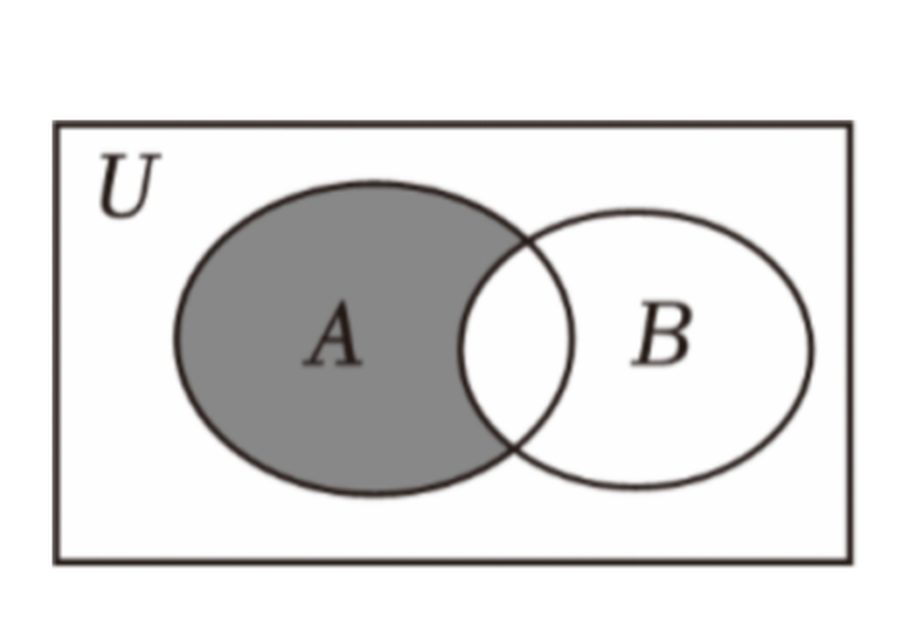
\includegraphics[width=0.34\textwidth]{figures/gao123_q17.png}
\end{center}

\ifanswer
\solbegin
\step{（1）$A\cap B=\{x\mid2\leqslant x\leqslant4\}$，}
\step{则图中阴影部分表示 $\overline{A\cap B}=\{x\mid-2\leqslant x<2\}$.}% 原卷把上划线盖在整个 $A\cap B$ 上，照录
\step{（2）由题意得 $\overline B=\{x\mid-6\leqslant x<2\}$，$C\subseteq B$，}
\step{所以当 $C=\varnothing$ 时，$10-a\geqslant2a+1$，解得 $a\leqslant3$，符合题意；}
\step{当 $C\neq\varnothing$ 时，$\begin{cases}10-a<2a+1\\2a+1\leqslant-6\end{cases}$ 或者 $\begin{cases}10-a<2a+1\\10-a\geqslant2\end{cases}$，}
\step{此时不等式组 $\begin{cases}10-a<2a+1\\2a+1\leqslant-6\end{cases}$ 无解，}
\step{不等式组 $\begin{cases}10-a<2a+1\\10-a\geqslant2\end{cases}$ 的解集为 $3<a\leqslant8$，}
\step{综上，$a$ 的取值范围为 $\{a\mid a\leqslant8\}$.}
\solend
\fi

\item (1) 求不等式：$\lvert x-1\rvert+\lvert x-2\rvert\leqslant5$ 的解集.

(2) 当 $m<1$ 时，解关于 $x$ 的不等式 $\dfrac{m(x-3)}{x+2}>1$.

\ifanswer
\solbegin
\step{(1) 当 $x<1$ 时，$\lvert x-1\rvert+\lvert x-2\rvert\leqslant5\Leftrightarrow-x+1+2-x\leqslant5$，}
\step{解得 $-1\leqslant x<1$；}
\step{当 $1\leqslant x\leqslant2$ 时，$\lvert x-1\rvert+\lvert x-2\rvert\leqslant5\Leftrightarrow x-1+2-x=1\leqslant5$ 恒成立，}
\step{所以 $1\leqslant x\leqslant2$；}
\step{当 $x>2$ 时，$\lvert x-1\rvert+\lvert x-2\rvert\leqslant5\Leftrightarrow x-1+x-2=2x-3\leqslant5$，}
\step{解得 $2<x\leqslant4$.}
\step{综上所述，不等式 $\lvert x-1\rvert+\lvert x-2\rvert\leqslant5$ 的解集为 $[-1,4]$.}
\step{(2) 原不等式变成 $\dfrac{(m-1)x-(3m+2)}{x+2}>0$，$n<1$，所以 $n-1<0$，}% 原卷作 $n<1$、$n-1<0$，与题设 $m<1$ 字母不一致，照录
\step{所以原不等式变成 $\dfrac{x-\dfrac{3m+2}{m-1}}{x+2}<0$，$\dfrac{3m+2}{m-1}-(-2)=\dfrac{5m}{m-1}$，}
\step{所以 $m<0$ 时，$\dfrac{5m}{m-1}>0$，$\dfrac{3m+2}{m-1}>-2$，}
\step{原不等式的解集为 $\left(-2,\dfrac{3m+2}{m-1}\right)$；}
\step{$m=0$ 时，原不等式变成 $1<0$，无解；}
\step{$0<m<1$ 时，$\dfrac{5m}{m-1}<0$，$\dfrac{3m+2}{m-1}<-2$，}
\step{原不等式的解集为 $\left(\dfrac{3m+2}{m-1},-2\right)$.}
\solend
\fi

\item 在园林博览会上，某公司带来了一种智能设备供采购商洽谈采购，并决定大量投放市场，已知该种设备年固定研发成本为 $50$ 万元，每生产一台需另投入 $100$ 元，设该公司一年内生产该设备 $x$ 万台且全部售完，每万台的销售收入 $G(x)$（万元）与年产量 $x$（万台）满足如下关系式：$G(x)=\begin{cases}180-x,0<x\leqslant20\\80+\dfrac{2000}{x}-\dfrac{8000}{x(x-1)},x>20\end{cases}$.

(1) 写出年利润 $W(x)$（万元）关于年产量 $x$（万台）的函数解析式；（利润 $=$ 销售收入 $-$ 成本）

(2) 当年产量为多少万台时，该公司获得的年利润最大，并求出最大利润.

\ifanswer
\solbegin
\step{(1) $W(x)=xG(x)-50-100x=\begin{cases}-50+80x-x^2,0<x\leqslant20\\-20x+1950-\dfrac{8000}{x-1},x>20\end{cases}$；}
\step{(2) 当 $0<x\leqslant20$ 时，$W(x)=-50+80x-x^2=-(x-40)^2+1550$，}
\step{由函数性质得当 $x\leqslant40$ 时严格增，所以当 $x=20$ 时，$W(x)_{max}=1150$，}
\step{当 $x>20$ 时，$W(x)=-20x+1950-\dfrac{8000}{x-1}=-20\left[(x-1)+\dfrac{400}{x-1}\right]+1930$，}
\step{$W(x)=-20\left[(x-1)+\dfrac{400}{x-1}\right]+1930\leqslant-20\times2\sqrt{(x-1)\cdot\dfrac{400}{x-1}}+1930$}
\step{$=1130$，当且仅当 $x-1=\dfrac{400}{x-1}$，即 $x=21$ 时取等号，}
\step{所以 $W(x)_{max}=1130$，}
\step{因为 $1150>1130$，所以当 $x=20$ 时，$W(x)_{max}=1150$，}
\step{即当年产量为 $20$ 万台时，该公司获得的年利润最大，}
\step{最大利润为 $1150$ 万元.}
\solend
\fi

\item 关于 $x$ 的方程 $(x^2-1)^2-2k\lvert x^2-1\rvert+k+1=0(k\in\R)$.

(1) 若方程无实根，求 $k$ 的取值范围；

(2) 若方程有 $4$ 个不等实根，求 $k$ 的取值范围；

(3) 若 $k=a+b$，且满足 $\dfrac1{a+2b}+\dfrac1{a+3}=\dfrac12$，$a>0$，$b>0$，试判断方程根的个数.

\ifanswer
\solbegin
\step{(1) 关于 $x$ 的方程 $(x^2-1)^2-2k\lvert x^2-1\rvert+k+1=0(k\in\R)$，}
\step{令 $t=\lvert x^2-1\rvert$，则 $t\geqslant0$，则原方程转化为 $t^2-2kt+k+1=0(*)$，}
\step{因为关于 $x$ 的方程 $(x^2-1)^2-2k\lvert x^2-1\rvert+k+1=0(k\in\R)$ 无实根，}
\step{所以 $(*)$ 式无实根或实根均小于零，令 $f(t)=t^2-2kt+k+1$，}
\step{①若 $(*)$ 式无实根，则 $\triangle<0$，解得 $\dfrac{1-\sqrt5}{2}<k<\dfrac{1+\sqrt5}{2}$，}
\step{②两根均为负，则 $\begin{cases}\Delta\geqslant0\\t_{\text{对}}=k<0\\f(0)>0\end{cases}$，解得 $-1<k\leqslant\dfrac{1-\sqrt5}{2}$，}
\step{综合①②，得 $k$ 的取值范围是 $\left(-1,\dfrac{1+\sqrt5}{2}\right)$；}
\step{(2) 作函数 $t=\lvert x^2-1\rvert$ 的图象，}
\begin{center}
% 图取原卷截图（第 11 页解析内）、去水印后 2× LANCZOS 放大，仅答案版出
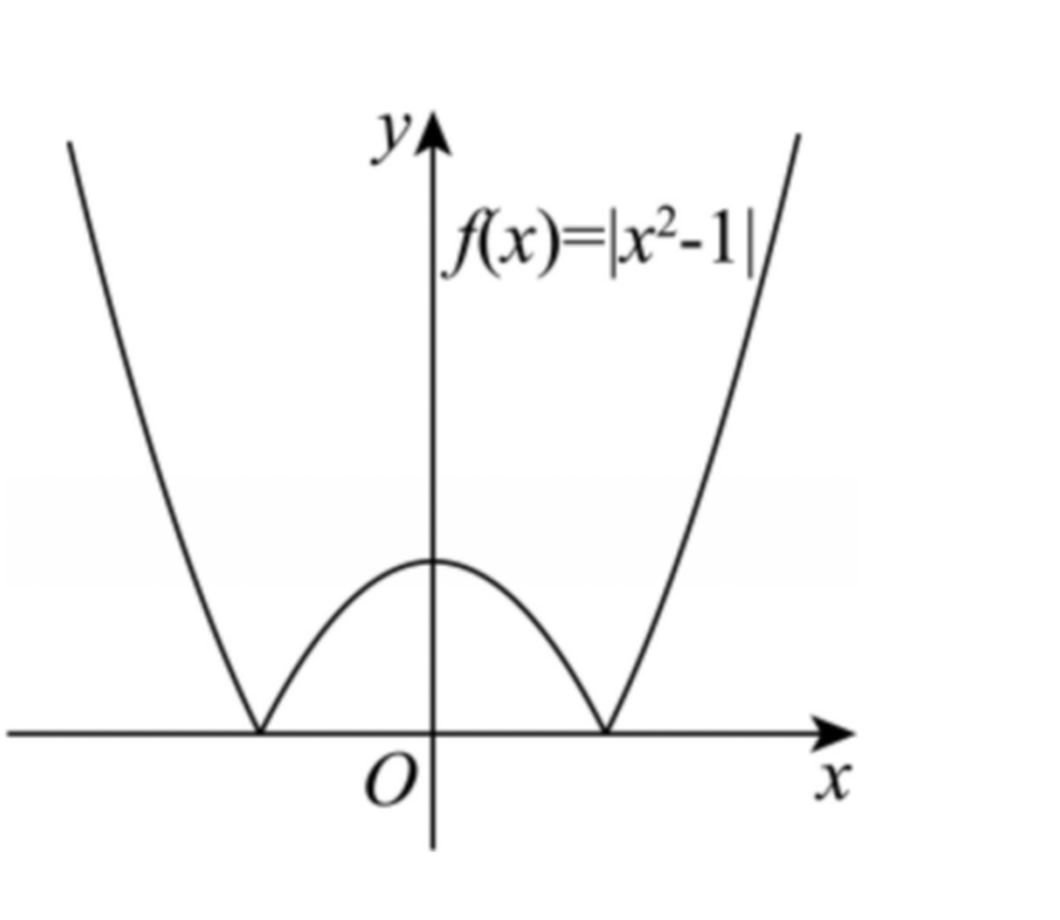
\includegraphics[width=0.40\textwidth]{figures/gao123_q20.png}
\end{center}
\step{$t=0$ 或 $t>1$ 时，每一个 $t$ 值对应 $2$ 个不同的 $x$ 值，}
\step{$t=1$ 时一个 $t$ 值对应 $3$ 个不同的 $x$ 值，}
\step{$0<t<1$ 时一个 $t$ 值对应 $4$ 个不同的 $x$ 值，}
\step{要使原方程有四个不等实根，}
\step{①$(*)$ 式一根为零，另一根大于 $1$，无解；}
\step{②$(*)$ 有两不等根且两根均大于 $1$，则 $\begin{cases}\Delta>0\\t_{\text{对}}=k>1\\f(1)>0\end{cases}$，解得 $\dfrac{1+\sqrt5}{2}<k<2$；}
\step{④$(*)$ 式有 $1$ 实根在 $(0,1)$ 之间，另一根小于零，}% 原卷由 ② 直接跳到 ④，缺 ③，照录
\step{则 $\begin{cases}f(0)<0\\f(1)>0\end{cases}$，所以 $\begin{cases}k+1<0\\2-k>0\end{cases}$，解得 $k<-1$，}
\step{综上所述，$k$ 取值范围为 $(-\infty,-1)\cup\left(\dfrac{1+\sqrt5}{2},2\right)$；}
\step{(3) 因为 $\dfrac1{a+2b}+\dfrac1{a+3}=\dfrac{a+2b+a+3}{(a+2b)(a+3)}=\dfrac{2(a+b)+3}{(a+2b)(a+3)}=\dfrac12$，}
\step{所以 $2(a+b)+3=\dfrac12(a+2b)(a+3)$，}
\step{因为 $a$、$b$ 为正实数，所以 $\dfrac12=\dfrac1{a+2b}+\dfrac1{a+3}\geqslant2\sqrt{\dfrac1{a+2b}\times\dfrac1{a+3}}$，}
\step{得 $\dfrac1{16}\geqslant\dfrac1{a+2b}\times\dfrac1{a+3}$，即 $(a+2b)(a+3)\geqslant16$，}
\step{所以 $2(a+b)+3\geqslant8$，即 $a+b\geqslant\dfrac52$，}
\step{当且仅当 $\dfrac1{a+2b}=\dfrac1{a+3}$ 即 $a=1$,$b=\dfrac32$ 时取等号，}
\step{故 $k\geqslant\dfrac52$，此时有 $\begin{cases}\Delta>0\\t_{\text{对}}=k>1\\f(0)>0,f(1)<0\end{cases}$，}
\step{故 $(*)$ 式有两不等实根且一根在 $(0,1)$ 之间，另一根大于 $1$，}
\step{故原方程有 $6$ 个实根.}
\solend
\fi

\item 设 $n$ 是不小于 $3$ 的正整数，集合 $S_n=\{(a_1,a_2,\cdots,a_n)\mid a_i\in\{0,1\},i=1,2,\cdots,n\}$，对于集合 $S_n$ 中任意两个元素 $A=(a_1,a_2,\cdots,a_n)$，$B=(b_1,b_2,\cdots,b_n)$.

定义 1：$A\cdot B=n-(\lvert a_1-b_1\rvert+\lvert a_2-b_2\rvert+\cdots+\lvert a_n-b_n\rvert)$，

定义 2：若 $A\cdot B=0$，则称互为相反元素，记作 $A=\overline B$ 或 $B=\overline A$.

(1) 若 $n=3$，$A=(0,1,0)$，$B=(1,1,0)$，试写出 $\overline A$、$\overline B$ 以及 $A\cdot B$ 的值；

(2) 若 $A$、$B\in S_n$，$A=(a_1,a_2,\cdots,a_n)$，$B=(b_1,b_2,\cdots,b_n)$，证明：$A\cdot B+\overline A\cdot B=n$；

(3) 设 $k$ 是小于 $n$ 的正奇数，至少含有两个元素的集合 $M\subseteq S_n$，且对于集合 $M$ 中任意两个不相同的元素 $A=(a_1,a_2,\cdots,a_n)$，$B=(b_1,b_2,\cdots,b_n)$，都有 $A\cdot B=n-k$，试求集合 $M$ 中元素个数的所有可能值.

\ifanswer
\solbegin
\step{(1) $\overline A=(1,0,1)$,$\overline B=(0,0,1)$,$\overline A\cdot\overline B=2$；}
\step{(2) 设 $A=(a_1,a_2,\cdots,a_n)$,$B=(b_1,b_2,\cdots,b_n)$,$\overline A=(x_1,x_2,\cdots,x_n)$，}
\step{由 $a_i$、$b_i$、$x_i\in\{0,1\}$，$i=1,2,\cdots,n$，得 $\lvert a_i-x_i\rvert\leqslant1$，$i=1,2,\cdots,n$，}
\step{所以 $\lvert a_1-x_1\rvert+\lvert a_2-x_2\rvert+\cdots+\lvert a_i-x_i\rvert\leqslant n$，}% 原卷末项下标作 $i$，照录
\step{当且仅当 $\lvert a_i-x_i\rvert=1$，$i=1,2,\cdots,n$，}
\step{即 $x_i=1-a_i$，$i=1,2,\cdots,n$ 时取等号.}
\step{由题意得 $A\cdot\overline A=n-(\lvert a_1-x_1\rvert+\lvert a_2-x_2\rvert+\cdots+\lvert a_n-x_n\rvert)=0$，}
\step{即 $\lvert a_1-x_1\rvert+\lvert a_2-x_2\rvert+\cdots+\lvert a_n-x_n\rvert=n$，}
\step{所以 $x_i=1-a_i$，$i=1,2,\cdots,n$，}
\step{$A\cdot B+\overline A\cdot B=2n-\sum\limits_{i=1}^n[\lvert a_i-b_i\rvert+(1-a_i)-b_i]$}
\step{$=2n-\sum\limits_{i=1}^n(\lvert1-b_i\rvert+\lvert0-b_i\rvert)=2n-\sum\limits_{i=1}^n(1-b_i+b_i)=2n-n=n$；}
\step{(3) 假设 $A=(a_1,a_2,\cdots,a_n)$，$B=(b_1,b_2,\cdots,b_n)$，$C=(c_1,c_2,\cdots,c_n)$}
\step{为集合 $M$ 中的三个不相同的元素，}
\step{则 $A\cdot B=n-(\lvert a_1-b_1\rvert+\lvert a_2-b_2\rvert+\cdots+\lvert a_n-b_n\rvert)=n-k$，}
\step{即 $\lvert a_1-b_1\rvert+\lvert a_2-b_2\rvert+\cdots+\lvert a_n-b_n\rvert=k$，}
\step{又由题意得 $\lvert a_i-b_i\rvert=0$ 或 $1$，$i=1,2,\cdots,n$，}
\step{$\lvert a_1-b_1\rvert$、$\lvert a_2-b_2\rvert$、$\cdots$、$\lvert a_n-b_n\rvert$ 恰有 $k$ 个 $1$，$n-k$ 个 $0$，}
\step{设其中 $k$ 个等于 $1$ 的项以此为 $a_{m_1}-b_{m_1}$,$a_{m_2}-b_{m_2}$,$\cdots$,$a_{m_k}-b_{m_k}$，}
\step{$n-k$ 个等于 $0$ 的项为 $a_{m_{k+1}}-b_{m_{k+1}}$,$a_{m_{k+2}}-b_{m_{k+2}}$,$\cdots$,$a_{m_n}-b_{m_n}$，}
\step{由题意得 $A\cdot C=n-(\lvert a_1-c_1\rvert+\lvert a_2-c_2\rvert+\cdots+\lvert a_n-c_n\rvert)=n-k$，}
\step{所以 $\sum\limits_{i=1}^k\lvert a_{m_i}-c_{m_i}\rvert+\sum\limits_{j=k+1}^n\lvert a_{m_j}-c_{m_j}\rvert=k$ ①，}
\step{同理 $\sum\limits_{i=1}^k\lvert b_{m_i}-c_{m_i}\rvert+\sum\limits_{j=k+1}^n\lvert b_{m_j}-c_{m_j}\rvert=k$ ②，}
\step{因为 $\lvert a_{m_{k+1}}-b_{m_{k+1}}\rvert=\lvert a_{m_{k+2}}-b_{m_{k+2}}\rvert=\cdots=\lvert a_{m_n}-b_{m_n}\rvert=0$，}
\step{所以 $\sum\limits_{j=k+1}^n\lvert a_{m_j}-c_{m_j}\rvert=\sum\limits_{j=k+1}^n\lvert b_{m_j}-c_{m_j}\rvert$，}
\step{由①$-$②得 $\sum\limits_{i=1}^k(\lvert a_{m_i}-c_{m_i}\rvert-\lvert b_{m_i}-c_{m_i}\rvert)=0$，}
\step{又 $\sum\limits_{i=1}^k(\lvert a_{m_i}-c_{m_i}\rvert-\lvert b_{m_i}-c_{m_i}\rvert)=\sum\limits_{i=1}^k(\lvert1-c_{m_i}\rvert-\lvert0-c_{m_i}\rvert)=k-2\sum\limits_{i=1}^k c_{m_i}$}
\step{为奇数，与 $\sum\limits_{i=1}^k(\lvert a_{m_i}-c_{m_i}\rvert-\lvert b_{m_i}-c_{m_i}\rvert)=0$ 矛盾，所以假设不成立，}
\step{即集合 $M$ 中至多有两个元素，}
\step{当 $M=\{(1,1,\cdots,1,0,0,\cdots,0),(0,0,\cdots,0)\}$ 时符合题意，}
\step{所以集合 $M$ 中元素的个数只可能是 $2$.}
\solend
\fi

\end{enumerate}

\end{document}
